\documentclass[twoside]{book}

% Packages required by doxygen
\usepackage{fixltx2e}
\usepackage{calc}
\usepackage{doxygen}
\usepackage[export]{adjustbox} % also loads graphicx
\usepackage{graphicx}
\usepackage[utf8]{inputenc}
\usepackage{makeidx}
\usepackage{multicol}
\usepackage{multirow}
\PassOptionsToPackage{warn}{textcomp}
\usepackage{textcomp}
\usepackage[nointegrals]{wasysym}
\usepackage[table]{xcolor}

% Font selection
\usepackage[T1]{fontenc}
\usepackage[scaled=.90]{helvet}
\usepackage{courier}
\usepackage{amssymb}
\usepackage{sectsty}
\renewcommand{\familydefault}{\sfdefault}
\allsectionsfont{%
  \fontseries{bc}\selectfont%
  \color{darkgray}%
}
\renewcommand{\DoxyLabelFont}{%
  \fontseries{bc}\selectfont%
  \color{darkgray}%
}
\newcommand{\+}{\discretionary{\mbox{\scriptsize$\hookleftarrow$}}{}{}}

% Page & text layout
\usepackage{geometry}
\geometry{%
  a4paper,%
  top=2.5cm,%
  bottom=2.5cm,%
  left=2.5cm,%
  right=2.5cm%
}
\tolerance=750
\hfuzz=15pt
\hbadness=750
\setlength{\emergencystretch}{15pt}
\setlength{\parindent}{0cm}
\setlength{\parskip}{3ex plus 2ex minus 2ex}
\makeatletter
\renewcommand{\paragraph}{%
  \@startsection{paragraph}{4}{0ex}{-1.0ex}{1.0ex}{%
    \normalfont\normalsize\bfseries\SS@parafont%
  }%
}
\renewcommand{\subparagraph}{%
  \@startsection{subparagraph}{5}{0ex}{-1.0ex}{1.0ex}{%
    \normalfont\normalsize\bfseries\SS@subparafont%
  }%
}
\makeatother

% Headers & footers
\usepackage{fancyhdr}
\pagestyle{fancyplain}
\fancyhead[LE]{\fancyplain{}{\bfseries\thepage}}
\fancyhead[CE]{\fancyplain{}{}}
\fancyhead[RE]{\fancyplain{}{\bfseries\leftmark}}
\fancyhead[LO]{\fancyplain{}{\bfseries\rightmark}}
\fancyhead[CO]{\fancyplain{}{}}
\fancyhead[RO]{\fancyplain{}{\bfseries\thepage}}
\fancyfoot[LE]{\fancyplain{}{}}
\fancyfoot[CE]{\fancyplain{}{}}
\fancyfoot[RE]{\fancyplain{}{\bfseries\scriptsize Generated by Doxygen }}
\fancyfoot[LO]{\fancyplain{}{\bfseries\scriptsize Generated by Doxygen }}
\fancyfoot[CO]{\fancyplain{}{}}
\fancyfoot[RO]{\fancyplain{}{}}
\renewcommand{\footrulewidth}{0.4pt}
\renewcommand{\chaptermark}[1]{%
  \markboth{#1}{}%
}
\renewcommand{\sectionmark}[1]{%
  \markright{\thesection\ #1}%
}

% Indices & bibliography
\usepackage{natbib}
\usepackage[titles]{tocloft}
\setcounter{tocdepth}{3}
\setcounter{secnumdepth}{5}
\makeindex

% Hyperlinks (required, but should be loaded last)
\usepackage{ifpdf}
\ifpdf
  \usepackage[pdftex,pagebackref=true]{hyperref}
\else
  \usepackage[ps2pdf,pagebackref=true]{hyperref}
\fi
\hypersetup{%
  colorlinks=true,%
  linkcolor=blue,%
  citecolor=blue,%
  unicode%
}

% Custom commands
\newcommand{\clearemptydoublepage}{%
  \newpage{\pagestyle{empty}\cleardoublepage}%
}

\usepackage{caption}
\captionsetup{labelsep=space,justification=centering,font={bf},singlelinecheck=off,skip=4pt,position=top}

%===== C O N T E N T S =====

\begin{document}

% Titlepage & ToC
\hypersetup{pageanchor=false,
             bookmarksnumbered=true,
             pdfencoding=unicode
            }
\pagenumbering{roman}
\begin{titlepage}
\vspace*{7cm}
\begin{center}%
{\Large Metronet }\\
\vspace*{1cm}
{\large Generated by Doxygen 1.8.11}\\
\end{center}
\end{titlepage}
\clearemptydoublepage
\tableofcontents
\clearemptydoublepage
\pagenumbering{arabic}
\hypersetup{pageanchor=true}

%--- Begin generated contents ---
\chapter{Deprecated List}
\label{deprecated}
\hypertarget{deprecated}{}

\begin{DoxyRefList}
\item[\label{deprecated__deprecated000002}%
\Hypertarget{deprecated__deprecated000002}%
Member \hyperlink{class_ti_xml_handle_ae9b22d71bf5f69ee5fda28f5ad21f19c}{Ti\+Xml\+Handle\+:\+:Element} () const]use To\+Element. Return the handle as a \hyperlink{class_ti_xml_element}{Ti\+Xml\+Element}. This may return null.  
\item[\label{deprecated__deprecated000001}%
\Hypertarget{deprecated__deprecated000001}%
Member \hyperlink{class_ti_xml_handle_aec0e3ea58ff98a45cd13507a02e2ca1e}{Ti\+Xml\+Handle\+:\+:Node} () const]use To\+Node. Return the handle as a \hyperlink{class_ti_xml_node}{Ti\+Xml\+Node}. This may return null.  
\item[\label{deprecated__deprecated000003}%
\Hypertarget{deprecated__deprecated000003}%
Member \hyperlink{class_ti_xml_handle_ad3b502c72059421e4dfcc7bda3c392fe}{Ti\+Xml\+Handle\+:\+:Text} () const]use \hyperlink{class_ti_xml_handle_abde286bce1d5db0d20ec30e573278cdf}{To\+Text()} Return the handle as a \hyperlink{class_ti_xml_text}{Ti\+Xml\+Text}. This may return null.  
\item[\label{deprecated__deprecated000004}%
\Hypertarget{deprecated__deprecated000004}%
Member \hyperlink{class_ti_xml_handle_a12b32f098c7daa5facbc04e9618262c5}{Ti\+Xml\+Handle\+:\+:Unknown} () const]use \hyperlink{class_ti_xml_handle_a450ec91dac1ded02d72eb918d062ad31}{To\+Unknown()} Return the handle as a \hyperlink{class_ti_xml_unknown}{Ti\+Xml\+Unknown}. This may return null. 
\end{DoxyRefList}
\chapter{Hierarchical Index}
\section{Class Hierarchy}
This inheritance list is sorted roughly, but not completely, alphabetically\+:\begin{DoxyCompactList}
\item \contentsline{section}{Exporter}{\pageref{class_exporter}}{}
\begin{DoxyCompactList}
\item \contentsline{section}{Exporter\+C\+LI}{\pageref{class_exporter_c_l_i}}{}
\item \contentsline{section}{Exporter\+H\+T\+ML}{\pageref{class_exporter_h_t_m_l}}{}
\item \contentsline{section}{Exporter\+T\+XT}{\pageref{class_exporter_t_x_t}}{}
\end{DoxyCompactList}
\item \contentsline{section}{Metronet}{\pageref{class_metronet}}{}
\item \contentsline{section}{Parser}{\pageref{class_parser}}{}
\item \contentsline{section}{Spoor}{\pageref{class_spoor}}{}
\item \contentsline{section}{Station}{\pageref{class_station}}{}
\item \contentsline{section}{Ti\+Xml\+Attribute\+Set}{\pageref{class_ti_xml_attribute_set}}{}
\item \contentsline{section}{Ti\+Xml\+Base}{\pageref{class_ti_xml_base}}{}
\begin{DoxyCompactList}
\item \contentsline{section}{Ti\+Xml\+Attribute}{\pageref{class_ti_xml_attribute}}{}
\item \contentsline{section}{Ti\+Xml\+Node}{\pageref{class_ti_xml_node}}{}
\begin{DoxyCompactList}
\item \contentsline{section}{Ti\+Xml\+Comment}{\pageref{class_ti_xml_comment}}{}
\item \contentsline{section}{Ti\+Xml\+Declaration}{\pageref{class_ti_xml_declaration}}{}
\item \contentsline{section}{Ti\+Xml\+Document}{\pageref{class_ti_xml_document}}{}
\item \contentsline{section}{Ti\+Xml\+Element}{\pageref{class_ti_xml_element}}{}
\item \contentsline{section}{Ti\+Xml\+Text}{\pageref{class_ti_xml_text}}{}
\item \contentsline{section}{Ti\+Xml\+Unknown}{\pageref{class_ti_xml_unknown}}{}
\end{DoxyCompactList}
\end{DoxyCompactList}
\item \contentsline{section}{Ti\+Xml\+Cursor}{\pageref{struct_ti_xml_cursor}}{}
\item \contentsline{section}{Ti\+Xml\+Handle}{\pageref{class_ti_xml_handle}}{}
\item \contentsline{section}{Ti\+Xml\+Parsing\+Data}{\pageref{class_ti_xml_parsing_data}}{}
\item \contentsline{section}{Ti\+Xml\+String}{\pageref{class_ti_xml_string}}{}
\begin{DoxyCompactList}
\item \contentsline{section}{Ti\+Xml\+Out\+Stream}{\pageref{class_ti_xml_out_stream}}{}
\end{DoxyCompactList}
\item \contentsline{section}{Ti\+Xml\+Visitor}{\pageref{class_ti_xml_visitor}}{}
\begin{DoxyCompactList}
\item \contentsline{section}{Ti\+Xml\+Printer}{\pageref{class_ti_xml_printer}}{}
\end{DoxyCompactList}
\item \contentsline{section}{Tram}{\pageref{class_tram}}{}
\end{DoxyCompactList}

\chapter{Class Index}
\section{Class List}
Here are the classes, structs, unions and interfaces with brief descriptions\+:\begin{DoxyCompactList}
\item\contentsline{section}{\hyperlink{class_exporter}{Exporter} }{\pageref{class_exporter}}{}
\item\contentsline{section}{\hyperlink{class_exporter_c_l_i}{Exporter\+C\+LI} }{\pageref{class_exporter_c_l_i}}{}
\item\contentsline{section}{\hyperlink{class_exporter_h_t_m_l}{Exporter\+H\+T\+ML} }{\pageref{class_exporter_h_t_m_l}}{}
\item\contentsline{section}{\hyperlink{class_exporter_t_x_t}{Exporter\+T\+XT} }{\pageref{class_exporter_t_x_t}}{}
\item\contentsline{section}{\hyperlink{class_metronet}{Metronet} }{\pageref{class_metronet}}{}
\item\contentsline{section}{\hyperlink{class_parser}{Parser} }{\pageref{class_parser}}{}
\item\contentsline{section}{\hyperlink{class_spoor}{Spoor} }{\pageref{class_spoor}}{}
\item\contentsline{section}{\hyperlink{class_station}{Station} }{\pageref{class_station}}{}
\item\contentsline{section}{\hyperlink{class_tram}{Tram} }{\pageref{class_tram}}{}
\end{DoxyCompactList}

\chapter{File Index}
\section{File List}
Here is a list of all files with brief descriptions\+:\begin{DoxyCompactList}
\item\contentsline{section}{/home/jonathan/\+Desktop/\+Project Software Engineering/\+Metronet/\+P\+S\+E/src/\hyperlink{_design_by_contract_8h}{Design\+By\+Contract.\+h} }{\pageref{_design_by_contract_8h}}{}
\item\contentsline{section}{/home/jonathan/\+Desktop/\+Project Software Engineering/\+Metronet/\+P\+S\+E/src/\hyperlink{_exporter_8cpp}{Exporter.\+cpp} }{\pageref{_exporter_8cpp}}{}
\item\contentsline{section}{/home/jonathan/\+Desktop/\+Project Software Engineering/\+Metronet/\+P\+S\+E/src/\hyperlink{_exporter_8h}{Exporter.\+h} }{\pageref{_exporter_8h}}{}
\item\contentsline{section}{/home/jonathan/\+Desktop/\+Project Software Engineering/\+Metronet/\+P\+S\+E/src/\hyperlink{main_8cpp}{main.\+cpp} }{\pageref{main_8cpp}}{}
\item\contentsline{section}{/home/jonathan/\+Desktop/\+Project Software Engineering/\+Metronet/\+P\+S\+E/src/\hyperlink{_metronet_8cpp}{Metronet.\+cpp} }{\pageref{_metronet_8cpp}}{}
\item\contentsline{section}{/home/jonathan/\+Desktop/\+Project Software Engineering/\+Metronet/\+P\+S\+E/src/\hyperlink{_metronet_8h}{Metronet.\+h} }{\pageref{_metronet_8h}}{}
\item\contentsline{section}{/home/jonathan/\+Desktop/\+Project Software Engineering/\+Metronet/\+P\+S\+E/src/\hyperlink{_metronet__test_8cpp}{Metronet\+\_\+test.\+cpp} }{\pageref{_metronet__test_8cpp}}{}
\item\contentsline{section}{/home/jonathan/\+Desktop/\+Project Software Engineering/\+Metronet/\+P\+S\+E/src/\hyperlink{_metronet_domain_test_8cpp}{Metronet\+Domain\+Test.\+cpp} }{\pageref{_metronet_domain_test_8cpp}}{}
\item\contentsline{section}{/home/jonathan/\+Desktop/\+Project Software Engineering/\+Metronet/\+P\+S\+E/src/\hyperlink{_metronet_domain_test_8h}{Metronet\+Domain\+Test.\+h} }{\pageref{_metronet_domain_test_8h}}{}
\item\contentsline{section}{/home/jonathan/\+Desktop/\+Project Software Engineering/\+Metronet/\+P\+S\+E/src/\hyperlink{_metronet_input_test_8cpp}{Metronet\+Input\+Test.\+cpp} }{\pageref{_metronet_input_test_8cpp}}{}
\item\contentsline{section}{/home/jonathan/\+Desktop/\+Project Software Engineering/\+Metronet/\+P\+S\+E/src/\hyperlink{_metronet_input_test_8h}{Metronet\+Input\+Test.\+h} }{\pageref{_metronet_input_test_8h}}{}
\item\contentsline{section}{/home/jonathan/\+Desktop/\+Project Software Engineering/\+Metronet/\+P\+S\+E/src/\hyperlink{_metronet_output_test_8cpp}{Metronet\+Output\+Test.\+cpp} }{\pageref{_metronet_output_test_8cpp}}{}
\item\contentsline{section}{/home/jonathan/\+Desktop/\+Project Software Engineering/\+Metronet/\+P\+S\+E/src/\hyperlink{_metronet_output_test_8h}{Metronet\+Output\+Test.\+h} }{\pageref{_metronet_output_test_8h}}{}
\item\contentsline{section}{/home/jonathan/\+Desktop/\+Project Software Engineering/\+Metronet/\+P\+S\+E/src/\hyperlink{_metronet_utils_8cpp}{Metronet\+Utils.\+cpp} }{\pageref{_metronet_utils_8cpp}}{}
\item\contentsline{section}{/home/jonathan/\+Desktop/\+Project Software Engineering/\+Metronet/\+P\+S\+E/src/\hyperlink{_metronet_utils_8h}{Metronet\+Utils.\+h} }{\pageref{_metronet_utils_8h}}{}
\item\contentsline{section}{/home/jonathan/\+Desktop/\+Project Software Engineering/\+Metronet/\+P\+S\+E/src/\hyperlink{_station_8cpp}{Station.\+cpp} }{\pageref{_station_8cpp}}{}
\item\contentsline{section}{/home/jonathan/\+Desktop/\+Project Software Engineering/\+Metronet/\+P\+S\+E/src/\hyperlink{_station_8h}{Station.\+h} }{\pageref{_station_8h}}{}
\item\contentsline{section}{/home/jonathan/\+Desktop/\+Project Software Engineering/\+Metronet/\+P\+S\+E/src/\hyperlink{_station__test_8cpp}{Station\+\_\+test.\+cpp} }{\pageref{_station__test_8cpp}}{}
\item\contentsline{section}{/home/jonathan/\+Desktop/\+Project Software Engineering/\+Metronet/\+P\+S\+E/src/\hyperlink{_tram_8cpp}{Tram.\+cpp} }{\pageref{_tram_8cpp}}{}
\item\contentsline{section}{/home/jonathan/\+Desktop/\+Project Software Engineering/\+Metronet/\+P\+S\+E/src/\hyperlink{_tram_8h}{Tram.\+h} }{\pageref{_tram_8h}}{}
\item\contentsline{section}{/home/jonathan/\+Desktop/\+Project Software Engineering/\+Metronet/\+P\+S\+E/src/\hyperlink{_tram__test_8cpp}{Tram\+\_\+test.\+cpp} }{\pageref{_tram__test_8cpp}}{}
\end{DoxyCompactList}

\chapter{Class Documentation}
\hypertarget{class_exporter}{}\section{Exporter Class Reference}
\label{class_exporter}\index{Exporter@{Exporter}}


\hyperlink{class_exporter}{Exporter} base klasse die de output van gegevens behandelt.  




{\ttfamily \#include $<$Exporter.\+h$>$}



Inheritance diagram for Exporter\+:
\nopagebreak
\begin{figure}[H]
\begin{center}
\leavevmode
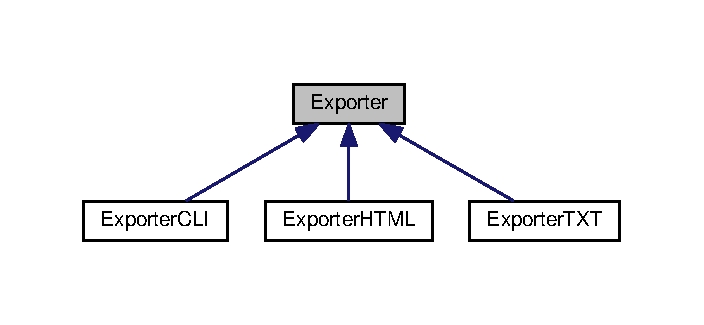
\includegraphics[width=350pt]{class_exporter__inherit__graph}
\end{center}
\end{figure}


Collaboration diagram for Exporter\+:
\nopagebreak
\begin{figure}[H]
\begin{center}
\leavevmode
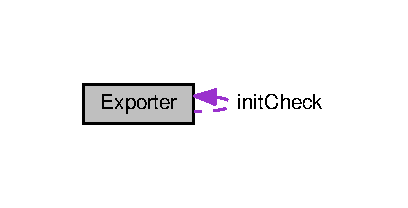
\includegraphics[width=204pt]{class_exporter__coll__graph}
\end{center}
\end{figure}
\subsection*{Public Member Functions}
\begin{DoxyCompactItemize}
\item 
\hyperlink{class_exporter_a2a977cb5ac8f637fcb570e73f650eca0}{Exporter} ()
\begin{DoxyCompactList}\small\item\em Lege constructor van \hyperlink{class_exporter}{Exporter}. \end{DoxyCompactList}\item 
bool \hyperlink{class_exporter_afba4e69e23ad018c26b21c0f4b85ef12}{is\+Document\+Started} () const 
\begin{DoxyCompactList}\small\item\em Getter van member document\+Started. \end{DoxyCompactList}\item 
virtual bool \hyperlink{class_exporter_af01d2a6c2f54329b1867a19537e11a34}{properly\+Initialised} () const 
\begin{DoxyCompactList}\small\item\em Kijk na of de constructor in de juiste staat geeindigd is. \end{DoxyCompactList}\item 
virtual void \hyperlink{class_exporter_ab3736803133eb727cf87a7306f91eb11}{write} (std\+::string \&output, std\+::ostream \&os)
\begin{DoxyCompactList}\small\item\em Stuur de output string naar de output stream. \end{DoxyCompactList}\item 
virtual void \hyperlink{class_exporter_ae477714f462d70cfc5b3970f91fcc4ed}{finish} (std\+::ostream \&os)
\begin{DoxyCompactList}\small\item\em Stuurt de nodige informatie naar de output stream om het document correct af te sluiten. \end{DoxyCompactList}\end{DoxyCompactItemize}
\subsection*{Protected Attributes}
\begin{DoxyCompactItemize}
\item 
bool \hyperlink{class_exporter_a7d55f6023d5fe983512f6b02fb60733b}{document\+Started}
\item 
\hyperlink{class_exporter}{Exporter} $\ast$ \hyperlink{class_exporter_a74245e988d8e72a43704dda927acff05}{init\+Check}
\end{DoxyCompactItemize}


\subsection{Detailed Description}
\hyperlink{class_exporter}{Exporter} base klasse die de output van gegevens behandelt. 

\subsection{Constructor \& Destructor Documentation}
\index{Exporter@{Exporter}!Exporter@{Exporter}}
\index{Exporter@{Exporter}!Exporter@{Exporter}}
\subsubsection[{\texorpdfstring{Exporter()}{Exporter()}}]{\setlength{\rightskip}{0pt plus 5cm}Exporter\+::\+Exporter (
\begin{DoxyParamCaption}
{}
\end{DoxyParamCaption}
)}\hypertarget{class_exporter_a2a977cb5ac8f637fcb570e73f650eca0}{}\label{class_exporter_a2a977cb5ac8f637fcb570e73f650eca0}


Lege constructor van \hyperlink{class_exporter}{Exporter}. 



\subsection{Member Function Documentation}
\index{Exporter@{Exporter}!finish@{finish}}
\index{finish@{finish}!Exporter@{Exporter}}
\subsubsection[{\texorpdfstring{finish(std\+::ostream \&os)}{finish(std::ostream &os)}}]{\setlength{\rightskip}{0pt plus 5cm}void Exporter\+::finish (
\begin{DoxyParamCaption}
\item[{std\+::ostream \&}]{os}
\end{DoxyParamCaption}
)\hspace{0.3cm}{\ttfamily [virtual]}}\hypertarget{class_exporter_ae477714f462d70cfc5b3970f91fcc4ed}{}\label{class_exporter_ae477714f462d70cfc5b3970f91fcc4ed}


Stuurt de nodige informatie naar de output stream om het document correct af te sluiten. 


\begin{DoxyParams}{Parameters}
{\em os} & De stream waar de output naar gestuurd zal worden. \\
\hline
\end{DoxyParams}
\begin{DoxyPrecond}{Precondition}
R\+E\+Q\+U\+I\+RE(this-\/$>$\hyperlink{class_exporter_af01d2a6c2f54329b1867a19537e11a34}{properly\+Initialised()}, \char`\"{}\+Exporter was niet geinitialiseerd bij de aanroep van finish.\char`\"{}); 

R\+E\+Q\+U\+I\+RE(document\+Started, \char`\"{}\+Document was niet aangemaakt voor de aanroep van finish.\char`\"{}); 
\end{DoxyPrecond}


Reimplemented in \hyperlink{class_exporter_h_t_m_l_aefa1c658f3c3c55bd7725bdad09629b3}{Exporter\+H\+T\+ML}.



Here is the call graph for this function\+:
\nopagebreak
\begin{figure}[H]
\begin{center}
\leavevmode
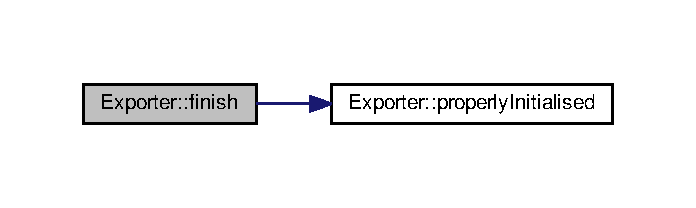
\includegraphics[width=350pt]{class_exporter_ae477714f462d70cfc5b3970f91fcc4ed_cgraph}
\end{center}
\end{figure}




Here is the caller graph for this function\+:
\nopagebreak
\begin{figure}[H]
\begin{center}
\leavevmode
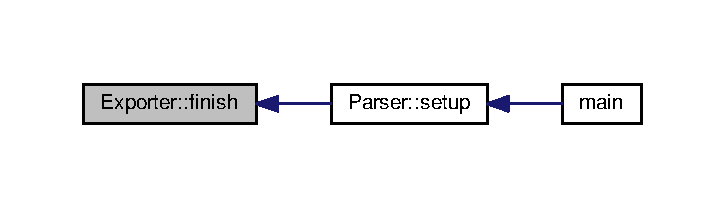
\includegraphics[width=263pt]{class_exporter_ae477714f462d70cfc5b3970f91fcc4ed_icgraph}
\end{center}
\end{figure}


\index{Exporter@{Exporter}!is\+Document\+Started@{is\+Document\+Started}}
\index{is\+Document\+Started@{is\+Document\+Started}!Exporter@{Exporter}}
\subsubsection[{\texorpdfstring{is\+Document\+Started() const }{isDocumentStarted() const }}]{\setlength{\rightskip}{0pt plus 5cm}bool Exporter\+::is\+Document\+Started (
\begin{DoxyParamCaption}
{}
\end{DoxyParamCaption}
) const}\hypertarget{class_exporter_afba4e69e23ad018c26b21c0f4b85ef12}{}\label{class_exporter_afba4e69e23ad018c26b21c0f4b85ef12}


Getter van member document\+Started. 

\begin{DoxyReturn}{Returns}
De waarde van document\+Started 
\end{DoxyReturn}
\begin{DoxyPrecond}{Precondition}
R\+E\+Q\+U\+I\+RE(this-\/$>$\hyperlink{class_exporter_af01d2a6c2f54329b1867a19537e11a34}{properly\+Initialised()}, \char`\"{}\+Exporter was niet geinitialiseerd bij de aanroep van is\+Document\+Started.\char`\"{}); 
\end{DoxyPrecond}


Here is the call graph for this function\+:
\nopagebreak
\begin{figure}[H]
\begin{center}
\leavevmode
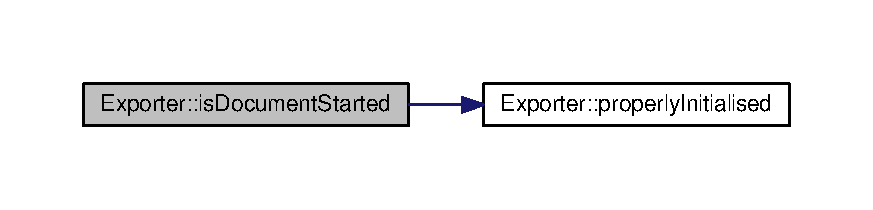
\includegraphics[width=350pt]{class_exporter_afba4e69e23ad018c26b21c0f4b85ef12_cgraph}
\end{center}
\end{figure}




Here is the caller graph for this function\+:
\nopagebreak
\begin{figure}[H]
\begin{center}
\leavevmode
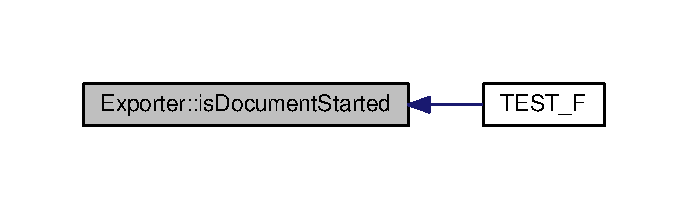
\includegraphics[width=330pt]{class_exporter_afba4e69e23ad018c26b21c0f4b85ef12_icgraph}
\end{center}
\end{figure}


\index{Exporter@{Exporter}!properly\+Initialised@{properly\+Initialised}}
\index{properly\+Initialised@{properly\+Initialised}!Exporter@{Exporter}}
\subsubsection[{\texorpdfstring{properly\+Initialised() const }{properlyInitialised() const }}]{\setlength{\rightskip}{0pt plus 5cm}bool Exporter\+::properly\+Initialised (
\begin{DoxyParamCaption}
{}
\end{DoxyParamCaption}
) const\hspace{0.3cm}{\ttfamily [virtual]}}\hypertarget{class_exporter_af01d2a6c2f54329b1867a19537e11a34}{}\label{class_exporter_af01d2a6c2f54329b1867a19537e11a34}


Kijk na of de constructor in de juiste staat geeindigd is. 

\begin{DoxyReturn}{Returns}
Boolean die aangeeft of het object juist geinitialiseerd is. 
\end{DoxyReturn}


Here is the caller graph for this function\+:
\nopagebreak
\begin{figure}[H]
\begin{center}
\leavevmode
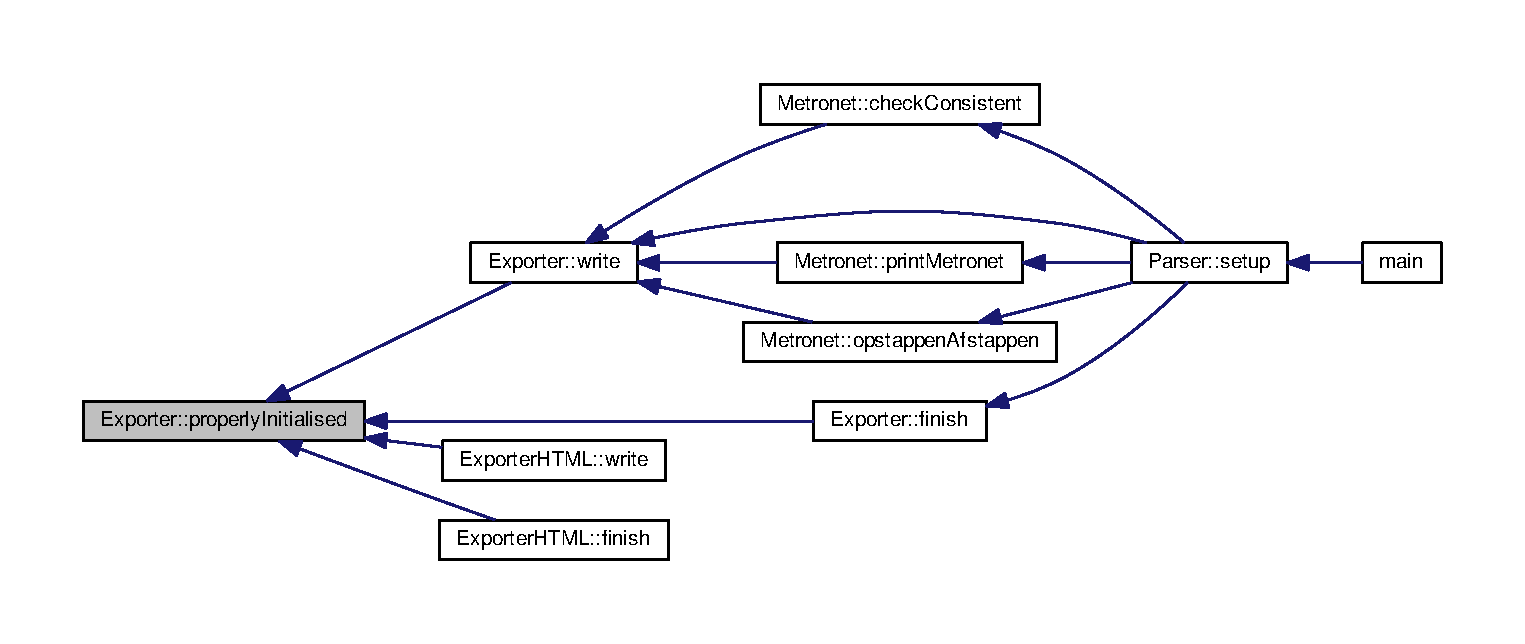
\includegraphics[width=350pt]{class_exporter_af01d2a6c2f54329b1867a19537e11a34_icgraph}
\end{center}
\end{figure}


\index{Exporter@{Exporter}!write@{write}}
\index{write@{write}!Exporter@{Exporter}}
\subsubsection[{\texorpdfstring{write(std\+::string \&output, std\+::ostream \&os)}{write(std::string &output, std::ostream &os)}}]{\setlength{\rightskip}{0pt plus 5cm}void Exporter\+::write (
\begin{DoxyParamCaption}
\item[{std\+::string \&}]{output, }
\item[{std\+::ostream \&}]{os}
\end{DoxyParamCaption}
)\hspace{0.3cm}{\ttfamily [virtual]}}\hypertarget{class_exporter_ab3736803133eb727cf87a7306f91eb11}{}\label{class_exporter_ab3736803133eb727cf87a7306f91eb11}


Stuur de output string naar de output stream. 


\begin{DoxyParams}{Parameters}
{\em output} & De string die naar de output gestuurd moet worden. \\
\hline
{\em os} & De stream waar de output naar gestuurd zal worden. \\
\hline
\end{DoxyParams}
\begin{DoxyPrecond}{Precondition}
R\+E\+Q\+U\+I\+RE(this-\/$>$\hyperlink{class_exporter_af01d2a6c2f54329b1867a19537e11a34}{properly\+Initialised()}, \char`\"{}\+Exporter was niet geinitialiseerd bij de aanroep van write.\char`\"{}); 
\end{DoxyPrecond}
\begin{DoxyPostcond}{Postcondition}
E\+N\+S\+U\+RE(document\+Started, \char`\"{}\+Document was niet aangemaakt bij de aanroep van write.\char`\"{}); 
\end{DoxyPostcond}


Reimplemented in \hyperlink{class_exporter_h_t_m_l_ace2649c240282289d4cb3bfbd19e427c}{Exporter\+H\+T\+ML}.



Here is the call graph for this function\+:
\nopagebreak
\begin{figure}[H]
\begin{center}
\leavevmode
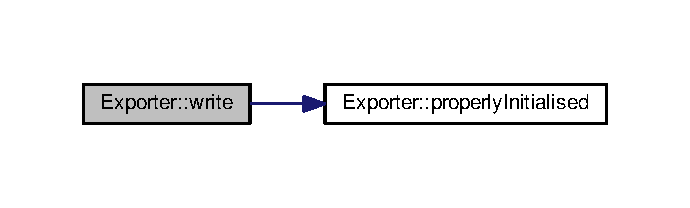
\includegraphics[width=350pt]{class_exporter_ab3736803133eb727cf87a7306f91eb11_cgraph}
\end{center}
\end{figure}




Here is the caller graph for this function\+:
\nopagebreak
\begin{figure}[H]
\begin{center}
\leavevmode
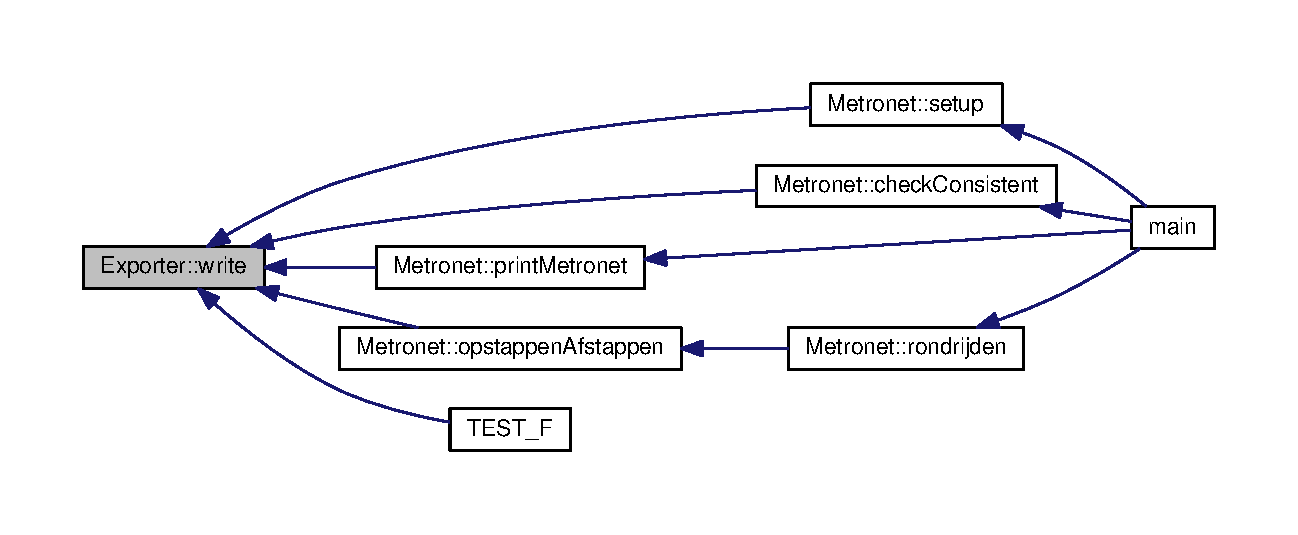
\includegraphics[width=350pt]{class_exporter_ab3736803133eb727cf87a7306f91eb11_icgraph}
\end{center}
\end{figure}




\subsection{Member Data Documentation}
\index{Exporter@{Exporter}!document\+Started@{document\+Started}}
\index{document\+Started@{document\+Started}!Exporter@{Exporter}}
\subsubsection[{\texorpdfstring{document\+Started}{documentStarted}}]{\setlength{\rightskip}{0pt plus 5cm}bool Exporter\+::document\+Started\hspace{0.3cm}{\ttfamily [protected]}}\hypertarget{class_exporter_a7d55f6023d5fe983512f6b02fb60733b}{}\label{class_exporter_a7d55f6023d5fe983512f6b02fb60733b}
\index{Exporter@{Exporter}!init\+Check@{init\+Check}}
\index{init\+Check@{init\+Check}!Exporter@{Exporter}}
\subsubsection[{\texorpdfstring{init\+Check}{initCheck}}]{\setlength{\rightskip}{0pt plus 5cm}{\bf Exporter}$\ast$ Exporter\+::init\+Check\hspace{0.3cm}{\ttfamily [protected]}}\hypertarget{class_exporter_a74245e988d8e72a43704dda927acff05}{}\label{class_exporter_a74245e988d8e72a43704dda927acff05}


The documentation for this class was generated from the following files\+:\begin{DoxyCompactItemize}
\item 
/home/jonathan/\+Desktop/\+Project Software Engineering/\+Metronet/\+P\+S\+E/src/\hyperlink{_exporter_8h}{Exporter.\+h}\item 
/home/jonathan/\+Desktop/\+Project Software Engineering/\+Metronet/\+P\+S\+E/src/\hyperlink{_exporter_8cpp}{Exporter.\+cpp}\end{DoxyCompactItemize}

\hypertarget{class_exporter_c_l_i}{}\section{Exporter\+C\+LI Class Reference}
\label{class_exporter_c_l_i}\index{Exporter\+C\+LI@{Exporter\+C\+LI}}


{\ttfamily \#include $<$Exporter.\+h$>$}



Inheritance diagram for Exporter\+C\+LI\+:\nopagebreak
\begin{figure}[H]
\begin{center}
\leavevmode
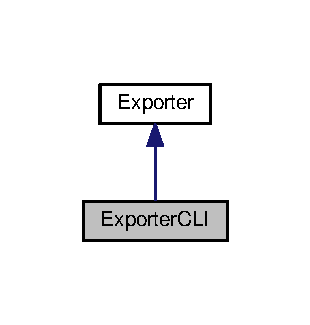
\includegraphics[width=149pt]{class_exporter_c_l_i__inherit__graph}
\end{center}
\end{figure}


Collaboration diagram for Exporter\+C\+LI\+:\nopagebreak
\begin{figure}[H]
\begin{center}
\leavevmode
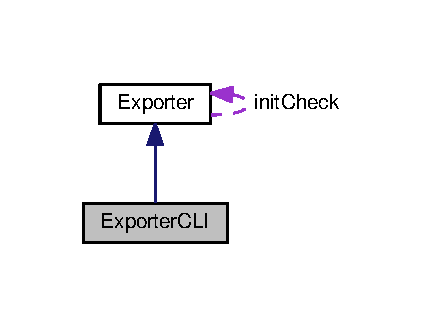
\includegraphics[width=204pt]{class_exporter_c_l_i__coll__graph}
\end{center}
\end{figure}
\subsection*{Additional Inherited Members}


The documentation for this class was generated from the following file\+:\begin{DoxyCompactItemize}
\item 
/home/jonathan/\+Desktop/\+Project Software Engineering/\+Metronet/\+P\+S\+E/src/\hyperlink{_exporter_8h}{Exporter.\+h}\end{DoxyCompactItemize}

\hypertarget{class_exporter_h_t_m_l}{}\section{Exporter\+H\+T\+ML Class Reference}
\label{class_exporter_h_t_m_l}\index{Exporter\+H\+T\+ML@{Exporter\+H\+T\+ML}}


{\ttfamily \#include $<$Exporter.\+h$>$}



Inheritance diagram for Exporter\+H\+T\+ML\+:
\nopagebreak
\begin{figure}[H]
\begin{center}
\leavevmode
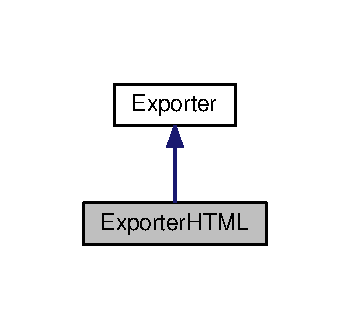
\includegraphics[width=160pt]{class_exporter_h_t_m_l__inherit__graph}
\end{center}
\end{figure}


Collaboration diagram for Exporter\+H\+T\+ML\+:
\nopagebreak
\begin{figure}[H]
\begin{center}
\leavevmode
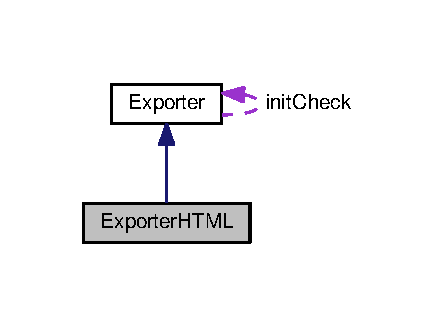
\includegraphics[width=160pt]{class_exporter_h_t_m_l__coll__graph}
\end{center}
\end{figure}
\subsection*{Public Member Functions}
\begin{DoxyCompactItemize}
\item 
virtual void \hyperlink{class_exporter_h_t_m_l_aa5b12621501f09a9a082e9337fbf943c}{write} (std\+::string \&output)
\begin{DoxyCompactList}\small\item\em Stuur de output string naar de output stream. \end{DoxyCompactList}\item 
virtual void \hyperlink{class_exporter_h_t_m_l_a60518b938e3cddd92ce3218de3651ac4}{validate} ()
\begin{DoxyCompactList}\small\item\em Valideer de output formaat. \end{DoxyCompactList}\item 
void \hyperlink{class_exporter_h_t_m_l_a2d9bb5e5f68a9e6111d8a929eb4a042e}{validate\+Head} ()
\begin{DoxyCompactList}\small\item\em Valideer de H\+T\+ML header. \end{DoxyCompactList}\item 
void \hyperlink{class_exporter_h_t_m_l_ab9d3ebcfa054f02f08ab34e1a6298963}{validate\+Tail} ()
\begin{DoxyCompactList}\small\item\em Valideer de H\+T\+ML tail. \end{DoxyCompactList}\end{DoxyCompactItemize}


\subsection{Member Function Documentation}
\index{Exporter\+H\+T\+ML@{Exporter\+H\+T\+ML}!validate@{validate}}
\index{validate@{validate}!Exporter\+H\+T\+ML@{Exporter\+H\+T\+ML}}
\subsubsection[{\texorpdfstring{validate()}{validate()}}]{\setlength{\rightskip}{0pt plus 5cm}void Exporter\+H\+T\+M\+L\+::validate (
\begin{DoxyParamCaption}
{}
\end{DoxyParamCaption}
)\hspace{0.3cm}{\ttfamily [virtual]}}\hypertarget{class_exporter_h_t_m_l_a60518b938e3cddd92ce3218de3651ac4}{}\label{class_exporter_h_t_m_l_a60518b938e3cddd92ce3218de3651ac4}


Valideer de output formaat. 

R\+E\+Q\+U\+I\+RE(this-\/$>$\hyperlink{class_exporter_af01d2a6c2f54329b1867a19537e11a34}{properly\+Initialised()}, \char`\"{}\+Exporter was niet geinitialiseerd bij de aanroep van validate,\char`\"{});~\newline
E\+N\+S\+U\+RE((document\+Started == true), \char`\"{}\+Document werd niet aangemaakt bij de aanroep van validate.\char`\"{});~\newline


Reimplemented from \hyperlink{class_exporter_a190fe737bcda2a55707ae51b731d11a5}{Exporter}.



Here is the call graph for this function\+:
\nopagebreak
\begin{figure}[H]
\begin{center}
\leavevmode
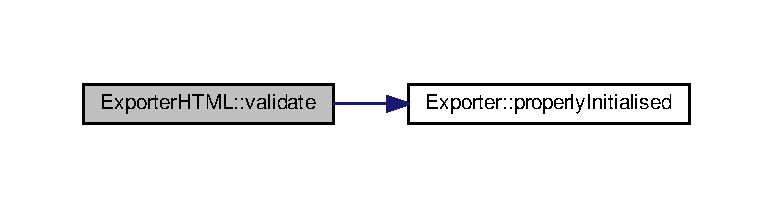
\includegraphics[width=350pt]{class_exporter_h_t_m_l_a60518b938e3cddd92ce3218de3651ac4_cgraph}
\end{center}
\end{figure}


\index{Exporter\+H\+T\+ML@{Exporter\+H\+T\+ML}!validate\+Head@{validate\+Head}}
\index{validate\+Head@{validate\+Head}!Exporter\+H\+T\+ML@{Exporter\+H\+T\+ML}}
\subsubsection[{\texorpdfstring{validate\+Head()}{validateHead()}}]{\setlength{\rightskip}{0pt plus 5cm}void Exporter\+H\+T\+M\+L\+::validate\+Head (
\begin{DoxyParamCaption}
{}
\end{DoxyParamCaption}
)}\hypertarget{class_exporter_h_t_m_l_a2d9bb5e5f68a9e6111d8a929eb4a042e}{}\label{class_exporter_h_t_m_l_a2d9bb5e5f68a9e6111d8a929eb4a042e}


Valideer de H\+T\+ML header. 

R\+E\+Q\+U\+I\+RE(this-\/$>$\hyperlink{class_exporter_af01d2a6c2f54329b1867a19537e11a34}{properly\+Initialised()}, \char`\"{}\+Exporter\+H\+T\+M\+L was niet geinitialiseerd bij het aanroepen van validate\+Head.\char`\"{});~\newline
R\+E\+Q\+U\+I\+RE(document\+Started == false), \char`\"{}\+Document was al aangemaakt voor de aanroep van validate\+Head.\char`\"{});~\newline
E\+N\+S\+U\+RE((document\+Started == true), \char`\"{}\+Document werd niet aangemaakt bij de aanroep van validate\+Head.\char`\"{});~\newline


Here is the call graph for this function\+:
\nopagebreak
\begin{figure}[H]
\begin{center}
\leavevmode
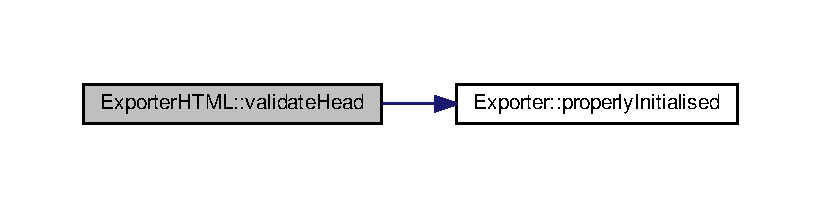
\includegraphics[width=350pt]{class_exporter_h_t_m_l_a2d9bb5e5f68a9e6111d8a929eb4a042e_cgraph}
\end{center}
\end{figure}


\index{Exporter\+H\+T\+ML@{Exporter\+H\+T\+ML}!validate\+Tail@{validate\+Tail}}
\index{validate\+Tail@{validate\+Tail}!Exporter\+H\+T\+ML@{Exporter\+H\+T\+ML}}
\subsubsection[{\texorpdfstring{validate\+Tail()}{validateTail()}}]{\setlength{\rightskip}{0pt plus 5cm}void Exporter\+H\+T\+M\+L\+::validate\+Tail (
\begin{DoxyParamCaption}
{}
\end{DoxyParamCaption}
)}\hypertarget{class_exporter_h_t_m_l_ab9d3ebcfa054f02f08ab34e1a6298963}{}\label{class_exporter_h_t_m_l_ab9d3ebcfa054f02f08ab34e1a6298963}


Valideer de H\+T\+ML tail. 

R\+E\+Q\+U\+I\+RE(this-\/$>$\hyperlink{class_exporter_af01d2a6c2f54329b1867a19537e11a34}{properly\+Initialised()}, \char`\"{}\+Exporter\+H\+T\+M\+L was niet geinitialiseerd bij het aanroepen van validate\+Tail.\char`\"{});~\newline
R\+E\+Q\+U\+I\+RE((document\+Started == true), \char`\"{}\+Document was nog niet aangemaakt bij de aanroep van validate\+Tail.\char`\"{}); E\+N\+S\+U\+RE((document\+Started == true), \char`\"{}\+Document werd niet aangemaakt bij de aanroep van validate\+Tail.\char`\"{});.~\newline


Here is the call graph for this function\+:
\nopagebreak
\begin{figure}[H]
\begin{center}
\leavevmode
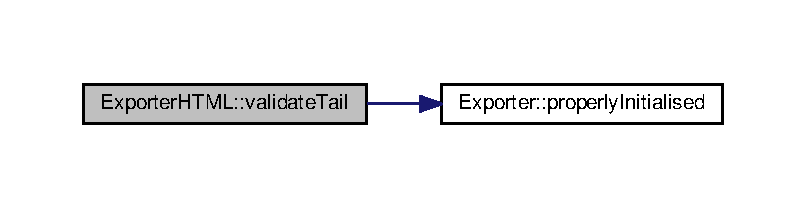
\includegraphics[width=350pt]{class_exporter_h_t_m_l_ab9d3ebcfa054f02f08ab34e1a6298963_cgraph}
\end{center}
\end{figure}


\index{Exporter\+H\+T\+ML@{Exporter\+H\+T\+ML}!write@{write}}
\index{write@{write}!Exporter\+H\+T\+ML@{Exporter\+H\+T\+ML}}
\subsubsection[{\texorpdfstring{write(std\+::string \&output)}{write(std::string &output)}}]{\setlength{\rightskip}{0pt plus 5cm}void Exporter\+H\+T\+M\+L\+::write (
\begin{DoxyParamCaption}
\item[{std\+::string \&}]{output}
\end{DoxyParamCaption}
)\hspace{0.3cm}{\ttfamily [virtual]}}\hypertarget{class_exporter_h_t_m_l_aa5b12621501f09a9a082e9337fbf943c}{}\label{class_exporter_h_t_m_l_aa5b12621501f09a9a082e9337fbf943c}


Stuur de output string naar de output stream. 


\begin{DoxyParams}{Parameters}
{\em output} & De string die naar de output gestuurd moet worden.\\
\hline
\end{DoxyParams}
R\+E\+Q\+U\+I\+RE(this-\/$>$\hyperlink{class_exporter_af01d2a6c2f54329b1867a19537e11a34}{properly\+Initialised()}, \char`\"{}\+Exporter was niet geinitialiseerd bij de aanroep van write.\char`\"{});~\newline


Reimplemented from \hyperlink{class_exporter_ac095b6486da16ffc76539f8c6c67be70}{Exporter}.



Here is the call graph for this function\+:
\nopagebreak
\begin{figure}[H]
\begin{center}
\leavevmode
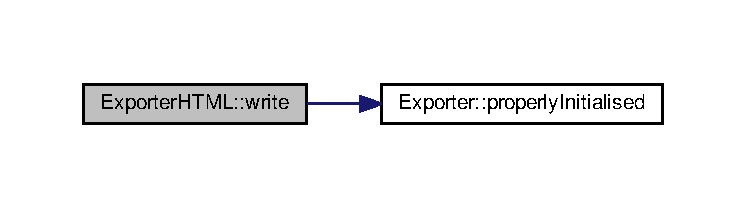
\includegraphics[width=350pt]{class_exporter_h_t_m_l_aa5b12621501f09a9a082e9337fbf943c_cgraph}
\end{center}
\end{figure}




The documentation for this class was generated from the following files\+:\begin{DoxyCompactItemize}
\item 
/home/jonathan/\+Desktop/\+Project Software Engineering/\+Metronet/\+P\+S\+E/src/\hyperlink{_exporter_8h}{Exporter.\+h}\item 
/home/jonathan/\+Desktop/\+Project Software Engineering/\+Metronet/\+P\+S\+E/src/\hyperlink{_exporter_8cpp}{Exporter.\+cpp}\end{DoxyCompactItemize}

\hypertarget{class_exporter_t_x_t}{}\section{Exporter\+T\+XT Class Reference}
\label{class_exporter_t_x_t}\index{Exporter\+T\+XT@{Exporter\+T\+XT}}


{\ttfamily \#include $<$Exporter.\+h$>$}



Inheritance diagram for Exporter\+T\+XT\+:
\nopagebreak
\begin{figure}[H]
\begin{center}
\leavevmode
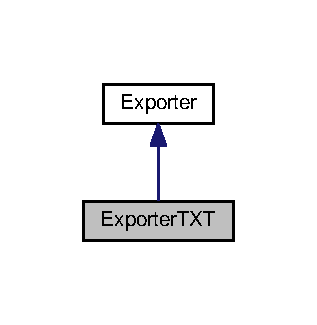
\includegraphics[width=152pt]{class_exporter_t_x_t__inherit__graph}
\end{center}
\end{figure}


Collaboration diagram for Exporter\+T\+XT\+:
\nopagebreak
\begin{figure}[H]
\begin{center}
\leavevmode
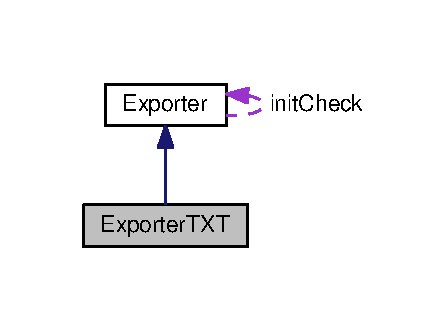
\includegraphics[width=152pt]{class_exporter_t_x_t__coll__graph}
\end{center}
\end{figure}
\subsection*{Additional Inherited Members}


The documentation for this class was generated from the following file\+:\begin{DoxyCompactItemize}
\item 
/home/jonathan/\+Desktop/\+Project Software Engineering/\+Metronet/\+P\+S\+E/src/\hyperlink{_exporter_8h}{Exporter.\+h}\end{DoxyCompactItemize}

\hypertarget{class_metronet}{}\section{Metronet Class Reference}
\label{class_metronet}\index{Metronet@{Metronet}}
\subsection*{Public Member Functions}
\begin{DoxyCompactItemize}
\item 
\mbox{\Hypertarget{class_metronet_a3d2adce29a947f162924279b766de645}\label{class_metronet_a3d2adce29a947f162924279b766de645}} 
bool \hyperlink{class_metronet_a3d2adce29a947f162924279b766de645}{properly\+Initialised} ()
\begin{DoxyCompactList}\small\item\em Kijk na of de constructor in de juiste staat geeindigd is. \end{DoxyCompactList}\item 
void \hyperlink{class_metronet_a37106294bf52324b0fb9fcecf11e5495}{add\+Station} (\hyperlink{class_station}{Station} $\ast$)
\begin{DoxyCompactList}\small\item\em Voegt station toe aan metronet. \end{DoxyCompactList}\item 
void \hyperlink{class_metronet_ab9bcc898b7b0ec5571ce149364cf64fc}{add\+Tram} (\hyperlink{class_tram}{Tram} $\ast$)
\begin{DoxyCompactList}\small\item\em Voegt tram toe aan metronet. \end{DoxyCompactList}\item 
void \hyperlink{class_metronet_ab6faa9e35828352e4003640d13798529}{add\+Spoor} (\hyperlink{class_spoor}{Spoor} $\ast$)
\begin{DoxyCompactList}\small\item\em Voegt spoor toe aan metronet. \end{DoxyCompactList}\item 
bool \hyperlink{class_metronet_a0128de167ec0a36e70abd57170b3faed}{check\+Consistent} (\hyperlink{class_exporter}{Exporter} $\ast$exp)
\begin{DoxyCompactList}\small\item\em Kijkt na of het metronet consistent is. \end{DoxyCompactList}\end{DoxyCompactItemize}


\subsection{Member Function Documentation}
\mbox{\Hypertarget{class_metronet_ab6faa9e35828352e4003640d13798529}\label{class_metronet_ab6faa9e35828352e4003640d13798529}} 
\index{Metronet@{Metronet}!add\+Spoor@{add\+Spoor}}
\index{add\+Spoor@{add\+Spoor}!Metronet@{Metronet}}
\subsubsection{\texorpdfstring{add\+Spoor()}{addSpoor()}}
{\footnotesize\ttfamily void Metronet\+::add\+Spoor (\begin{DoxyParamCaption}\item[{\hyperlink{class_spoor}{Spoor} $\ast$}]{spoor }\end{DoxyParamCaption})}



Voegt spoor toe aan metronet. 

R\+E\+Q\+U\+I\+RE(this-\/$>$\hyperlink{class_metronet_a3d2adce29a947f162924279b766de645}{properly\+Initialised()}, \char`\"{}\+Metronet was niet geinitialiseerd bij de aanroep van add\+Spoor.\char`\"{});~\newline
R\+E\+Q\+U\+I\+RE(Spoor-\/$>$\hyperlink{class_metronet_a3d2adce29a947f162924279b766de645}{properly\+Initialised()}, \char`\"{}\+Spoor was niet geinitialiseerd bij de aanroep van add\+Spoor.\char`\"{});~\newline
E\+N\+S\+U\+RE(sporen\mbox{[}sporen.\+size() -\/ 1\mbox{]} == \hyperlink{class_spoor}{Spoor}), \char`\"{}\+Spoor was niet toegevoegd bij de aanroep van add\+Spoor.\char`\"{});~\newline
\mbox{\Hypertarget{class_metronet_a37106294bf52324b0fb9fcecf11e5495}\label{class_metronet_a37106294bf52324b0fb9fcecf11e5495}} 
\index{Metronet@{Metronet}!add\+Station@{add\+Station}}
\index{add\+Station@{add\+Station}!Metronet@{Metronet}}
\subsubsection{\texorpdfstring{add\+Station()}{addStation()}}
{\footnotesize\ttfamily void Metronet\+::add\+Station (\begin{DoxyParamCaption}\item[{\hyperlink{class_station}{Station} $\ast$}]{station }\end{DoxyParamCaption})}



Voegt station toe aan metronet. 

R\+E\+Q\+U\+I\+RE(this-\/$>$\hyperlink{class_metronet_a3d2adce29a947f162924279b766de645}{properly\+Initialised()}, \char`\"{}\+Metronet was niet geinitialiseerd bij de aanroep van add\+Station.\char`\"{});~\newline
R\+E\+Q\+U\+I\+RE(Station-\/$>$\hyperlink{class_metronet_a3d2adce29a947f162924279b766de645}{properly\+Initialised()}, \char`\"{}\+Station was niet geinitialiseerd bij de aanroep van add\+Station.\char`\"{});~\newline
E\+N\+S\+U\+RE(stations\mbox{[}stations.\+size() -\/ 1\mbox{]} == \hyperlink{class_station}{Station}), \char`\"{}\+Station was niet toegevoegd bij de aanroep van add\+Station.\char`\"{});~\newline
\mbox{\Hypertarget{class_metronet_ab9bcc898b7b0ec5571ce149364cf64fc}\label{class_metronet_ab9bcc898b7b0ec5571ce149364cf64fc}} 
\index{Metronet@{Metronet}!add\+Tram@{add\+Tram}}
\index{add\+Tram@{add\+Tram}!Metronet@{Metronet}}
\subsubsection{\texorpdfstring{add\+Tram()}{addTram()}}
{\footnotesize\ttfamily void Metronet\+::add\+Tram (\begin{DoxyParamCaption}\item[{\hyperlink{class_tram}{Tram} $\ast$}]{tram }\end{DoxyParamCaption})}



Voegt tram toe aan metronet. 

R\+E\+Q\+U\+I\+RE(this-\/$>$\hyperlink{class_metronet_a3d2adce29a947f162924279b766de645}{properly\+Initialised()}, \char`\"{}\+Metronet was niet geinitialiseerd bij de aanroep van add\+Tram.\char`\"{});~\newline
R\+E\+Q\+U\+I\+RE(Tram-\/$>$\hyperlink{class_metronet_a3d2adce29a947f162924279b766de645}{properly\+Initialised()}, \char`\"{}\+Tram was niet geinitialiseerd bij de aanroep van add\+Tram.\char`\"{});~\newline
E\+N\+S\+U\+RE(trams\mbox{[}trams.\+size() -\/ 1\mbox{]} == \hyperlink{class_tram}{Tram}), \char`\"{}\+Tram was niet toegevoegd bij de aanroep van add\+Tram.\char`\"{});~\newline
\mbox{\Hypertarget{class_metronet_a0128de167ec0a36e70abd57170b3faed}\label{class_metronet_a0128de167ec0a36e70abd57170b3faed}} 
\index{Metronet@{Metronet}!check\+Consistent@{check\+Consistent}}
\index{check\+Consistent@{check\+Consistent}!Metronet@{Metronet}}
\subsubsection{\texorpdfstring{check\+Consistent()}{checkConsistent()}}
{\footnotesize\ttfamily bool Metronet\+::check\+Consistent (\begin{DoxyParamCaption}\item[{\hyperlink{class_exporter}{Exporter} $\ast$}]{exp }\end{DoxyParamCaption})}



Kijkt na of het metronet consistent is. 


\begin{DoxyParams}{Parameters}
{\em exp} & De exporter die de output zal behandelen. R\+E\+Q\+U\+I\+RE(this-\/$>$\hyperlink{class_metronet_a3d2adce29a947f162924279b766de645}{properly\+Initialised()}, \char`\"{}\+Metronet was niet geinitialiseerd bij de aanroep van check\+Consistent.\char`\"{});~\newline
\\
\hline
\end{DoxyParams}


The documentation for this class was generated from the following files\+:\begin{DoxyCompactItemize}
\item 
/home/sergio/\+C\+Lion\+Projects/\+Soft\+Eng/src/Metronet.\+h\item 
/home/sergio/\+C\+Lion\+Projects/\+Soft\+Eng/src/Metronet.\+cpp\end{DoxyCompactItemize}

\hypertarget{class_parser}{}\section{Parser Class Reference}
\label{class_parser}\index{Parser@{Parser}}


{\ttfamily \#include $<$Parser.\+h$>$}

\subsection*{Public Member Functions}
\begin{DoxyCompactItemize}
\item 
\hyperlink{class_parser_a12234f6cd36b61af4b50c94a179422c1}{Parser} ()
\item 
virtual \hyperlink{class_parser_a3e658b5917a93a3ef648050d060e3a93}{$\sim$\+Parser} ()
\end{DoxyCompactItemize}


\subsection{Constructor \& Destructor Documentation}
\mbox{\Hypertarget{class_parser_a12234f6cd36b61af4b50c94a179422c1}\label{class_parser_a12234f6cd36b61af4b50c94a179422c1}} 
\index{Parser@{Parser}!Parser@{Parser}}
\index{Parser@{Parser}!Parser@{Parser}}
\subsubsection{\texorpdfstring{Parser()}{Parser()}}
{\footnotesize\ttfamily Parser\+::\+Parser (\begin{DoxyParamCaption}{ }\end{DoxyParamCaption})}

\mbox{\Hypertarget{class_parser_a3e658b5917a93a3ef648050d060e3a93}\label{class_parser_a3e658b5917a93a3ef648050d060e3a93}} 
\index{Parser@{Parser}!````~Parser@{$\sim$\+Parser}}
\index{````~Parser@{$\sim$\+Parser}!Parser@{Parser}}
\subsubsection{\texorpdfstring{$\sim$\+Parser()}{~Parser()}}
{\footnotesize\ttfamily Parser\+::$\sim$\+Parser (\begin{DoxyParamCaption}{ }\end{DoxyParamCaption})\hspace{0.3cm}{\ttfamily [virtual]}}



The documentation for this class was generated from the following files\+:\begin{DoxyCompactItemize}
\item 
/home/sergio/\+Eclipse\+Projects/\+Soft\+Eng/src/\hyperlink{_parser_8h}{Parser.\+h}\item 
/home/sergio/\+Eclipse\+Projects/\+Soft\+Eng/src/\hyperlink{_parser_8cpp}{Parser.\+cpp}\end{DoxyCompactItemize}

\hypertarget{class_spoor}{}\section{Spoor Class Reference}
\label{class_spoor}\index{Spoor@{Spoor}}


{\ttfamily \#include $<$Spoor.\+h$>$}

\subsection*{Public Member Functions}
\begin{DoxyCompactItemize}
\item 
\hyperlink{class_spoor_a64778a4094d2d9cd3a08cbbef5a11787}{Spoor} ()
\item 
virtual \hyperlink{class_spoor_a58dcc52a48e4ad3ca7d9028a0065ca98}{$\sim$\+Spoor} ()
\item 
bool \hyperlink{class_spoor_a1eb7c54228676cdb7c8620104e063a3c}{properly\+Initialised} () const
\begin{DoxyCompactList}\small\item\em Kijk na of de constructor in de juiste staat geeindigd is. \end{DoxyCompactList}\item 
int \hyperlink{class_spoor_a66ebc0abcb370b1509bd7b3961a8e45a}{get\+Lijn\+Nr} () const
\begin{DoxyCompactList}\small\item\em Geef het lijn nummer terug. \end{DoxyCompactList}\end{DoxyCompactItemize}


\subsection{Constructor \& Destructor Documentation}
\mbox{\Hypertarget{class_spoor_a64778a4094d2d9cd3a08cbbef5a11787}\label{class_spoor_a64778a4094d2d9cd3a08cbbef5a11787}} 
\index{Spoor@{Spoor}!Spoor@{Spoor}}
\index{Spoor@{Spoor}!Spoor@{Spoor}}
\subsubsection{\texorpdfstring{Spoor()}{Spoor()}}
{\footnotesize\ttfamily Spoor\+::\+Spoor (\begin{DoxyParamCaption}{ }\end{DoxyParamCaption})}

\mbox{\Hypertarget{class_spoor_a58dcc52a48e4ad3ca7d9028a0065ca98}\label{class_spoor_a58dcc52a48e4ad3ca7d9028a0065ca98}} 
\index{Spoor@{Spoor}!````~Spoor@{$\sim$\+Spoor}}
\index{````~Spoor@{$\sim$\+Spoor}!Spoor@{Spoor}}
\subsubsection{\texorpdfstring{$\sim$\+Spoor()}{~Spoor()}}
{\footnotesize\ttfamily Spoor\+::$\sim$\+Spoor (\begin{DoxyParamCaption}{ }\end{DoxyParamCaption})\hspace{0.3cm}{\ttfamily [virtual]}}



\subsection{Member Function Documentation}
\mbox{\Hypertarget{class_spoor_a66ebc0abcb370b1509bd7b3961a8e45a}\label{class_spoor_a66ebc0abcb370b1509bd7b3961a8e45a}} 
\index{Spoor@{Spoor}!get\+Lijn\+Nr@{get\+Lijn\+Nr}}
\index{get\+Lijn\+Nr@{get\+Lijn\+Nr}!Spoor@{Spoor}}
\subsubsection{\texorpdfstring{get\+Lijn\+Nr()}{getLijnNr()}}
{\footnotesize\ttfamily int Spoor\+::get\+Lijn\+Nr (\begin{DoxyParamCaption}{ }\end{DoxyParamCaption}) const}



Geef het lijn nummer terug. 

\begin{DoxyReturn}{Returns}
Het aantal zitplaatsen.
\end{DoxyReturn}
R\+E\+Q\+U\+I\+RE(this-\/$>$\hyperlink{class_spoor_a1eb7c54228676cdb7c8620104e063a3c}{properly\+Initialised()}, \char`\"{}\+Spoor was niet geinitialiseerd bij de aanroep van get\+Lijn\+Nr.\char`\"{});~\newline
Here is the call graph for this function\+:\nopagebreak
\begin{figure}[H]
\begin{center}
\leavevmode
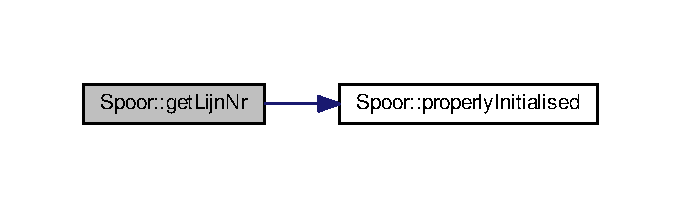
\includegraphics[width=327pt]{class_spoor_a66ebc0abcb370b1509bd7b3961a8e45a_cgraph}
\end{center}
\end{figure}
\mbox{\Hypertarget{class_spoor_a1eb7c54228676cdb7c8620104e063a3c}\label{class_spoor_a1eb7c54228676cdb7c8620104e063a3c}} 
\index{Spoor@{Spoor}!properly\+Initialised@{properly\+Initialised}}
\index{properly\+Initialised@{properly\+Initialised}!Spoor@{Spoor}}
\subsubsection{\texorpdfstring{properly\+Initialised()}{properlyInitialised()}}
{\footnotesize\ttfamily bool Spoor\+::properly\+Initialised (\begin{DoxyParamCaption}{ }\end{DoxyParamCaption}) const}



Kijk na of de constructor in de juiste staat geeindigd is. 

\begin{DoxyReturn}{Returns}
Boolean die aangeeft of het object juist geinitialiseerd is. 
\end{DoxyReturn}
Here is the caller graph for this function\+:\nopagebreak
\begin{figure}[H]
\begin{center}
\leavevmode
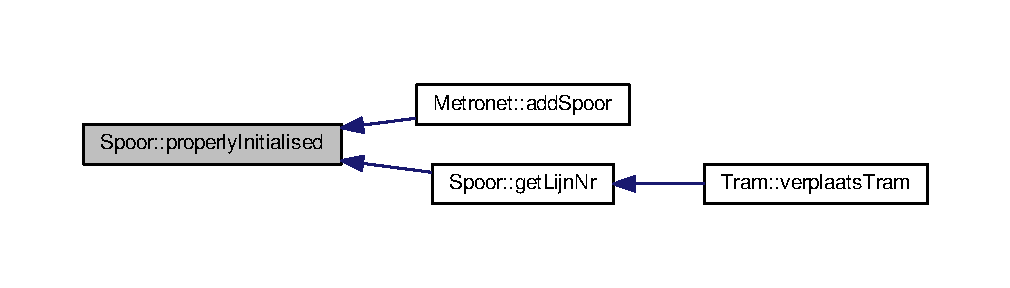
\includegraphics[width=342pt]{class_spoor_a1eb7c54228676cdb7c8620104e063a3c_icgraph}
\end{center}
\end{figure}


The documentation for this class was generated from the following files\+:\begin{DoxyCompactItemize}
\item 
/home/sergio/\+Eclipse\+Projects/\+Soft\+Eng/src/\hyperlink{_spoor_8h}{Spoor.\+h}\item 
/home/sergio/\+Eclipse\+Projects/\+Soft\+Eng/src/\hyperlink{_spoor_8cpp}{Spoor.\+cpp}\end{DoxyCompactItemize}

\hypertarget{class_station}{}\section{Station Class Reference}
\label{class_station}\index{Station@{Station}}


{\ttfamily \#include $<$Station.\+h$>$}

\subsection*{Public Member Functions}
\begin{DoxyCompactItemize}
\item 
\hyperlink{class_station_a73d335726aad1d844d81cda6d9fd74e6}{Station} ()
\item 
\hyperlink{class_station_a1685ff9a628b922fbc6a75f0f23c7b7e}{Station} (std\+::string n, \hyperlink{class_station}{Station} $\ast$vor, \hyperlink{class_station}{Station} $\ast$volg, \hyperlink{class_spoor}{Spoor} $\ast$sp)
\item 
virtual \hyperlink{class_station_a00434e79e8ee7f4ebd6d3b631dde5ac0}{$\sim$\+Station} ()
\item 
bool \hyperlink{class_station_a5749af84d13b71d34aa1fb5b0a935a20}{properly\+Initialised} () const 
\begin{DoxyCompactList}\small\item\em Kijk na of de constructor in de juiste staat geeindigd is. \end{DoxyCompactList}\item 
std\+::string \hyperlink{class_station_a6d4234bcd1027dc83c7984e207e8bd74}{get\+Naam} () const 
\begin{DoxyCompactList}\small\item\em Geef de naam terug van het station. \end{DoxyCompactList}\item 
\hyperlink{class_station}{Station} $\ast$ \hyperlink{class_station_a2adced993339721e8731bfa55762f4f9}{get\+Vorige} () const 
\begin{DoxyCompactList}\small\item\em Geef het vorig station terug. \end{DoxyCompactList}\item 
\hyperlink{class_station}{Station} $\ast$ \hyperlink{class_station_a2c81d14029f13b972c015a16813c8d34}{get\+Volgende} () const 
\begin{DoxyCompactList}\small\item\em Geef het volgende station. \end{DoxyCompactList}\item 
\hyperlink{class_spoor}{Spoor} $\ast$ \hyperlink{class_station_af7ea9d2ec05b56832c0e1a2fe2303ee1}{get\+Spoor} () const 
\begin{DoxyCompactList}\small\item\em Geef het \hyperlink{class_spoor}{Spoor} terug. \end{DoxyCompactList}\end{DoxyCompactItemize}


\subsection{Constructor \& Destructor Documentation}
\index{Station@{Station}!Station@{Station}}
\index{Station@{Station}!Station@{Station}}
\subsubsection[{\texorpdfstring{Station()}{Station()}}]{\setlength{\rightskip}{0pt plus 5cm}Station\+::\+Station (
\begin{DoxyParamCaption}
{}
\end{DoxyParamCaption}
)}\hypertarget{class_station_a73d335726aad1d844d81cda6d9fd74e6}{}\label{class_station_a73d335726aad1d844d81cda6d9fd74e6}
\index{Station@{Station}!Station@{Station}}
\index{Station@{Station}!Station@{Station}}
\subsubsection[{\texorpdfstring{Station(std\+::string n, Station $\ast$vor, Station $\ast$volg, Spoor $\ast$sp)}{Station(std::string n, Station *vor, Station *volg, Spoor *sp)}}]{\setlength{\rightskip}{0pt plus 5cm}Station\+::\+Station (
\begin{DoxyParamCaption}
\item[{std\+::string}]{n, }
\item[{{\bf Station} $\ast$}]{vor, }
\item[{{\bf Station} $\ast$}]{volg, }
\item[{{\bf Spoor} $\ast$}]{sp}
\end{DoxyParamCaption}
)}\hypertarget{class_station_a1685ff9a628b922fbc6a75f0f23c7b7e}{}\label{class_station_a1685ff9a628b922fbc6a75f0f23c7b7e}
\index{Station@{Station}!````~Station@{$\sim$\+Station}}
\index{````~Station@{$\sim$\+Station}!Station@{Station}}
\subsubsection[{\texorpdfstring{$\sim$\+Station()}{~Station()}}]{\setlength{\rightskip}{0pt plus 5cm}Station\+::$\sim$\+Station (
\begin{DoxyParamCaption}
{}
\end{DoxyParamCaption}
)\hspace{0.3cm}{\ttfamily [virtual]}}\hypertarget{class_station_a00434e79e8ee7f4ebd6d3b631dde5ac0}{}\label{class_station_a00434e79e8ee7f4ebd6d3b631dde5ac0}


\subsection{Member Function Documentation}
\index{Station@{Station}!get\+Naam@{get\+Naam}}
\index{get\+Naam@{get\+Naam}!Station@{Station}}
\subsubsection[{\texorpdfstring{get\+Naam() const }{getNaam() const }}]{\setlength{\rightskip}{0pt plus 5cm}std\+::string Station\+::get\+Naam (
\begin{DoxyParamCaption}
{}
\end{DoxyParamCaption}
) const}\hypertarget{class_station_a6d4234bcd1027dc83c7984e207e8bd74}{}\label{class_station_a6d4234bcd1027dc83c7984e207e8bd74}


Geef de naam terug van het station. 

\begin{DoxyReturn}{Returns}
De naam van het station.
\end{DoxyReturn}
R\+E\+Q\+U\+I\+RE(this-\/$>$\hyperlink{class_station_a5749af84d13b71d34aa1fb5b0a935a20}{properly\+Initialised()}, \char`\"{}\+Station was niet geinitialiseerd bij de aanroep van get\+Naam.\char`\"{});~\newline


Here is the call graph for this function\+:
\nopagebreak
\begin{figure}[H]
\begin{center}
\leavevmode
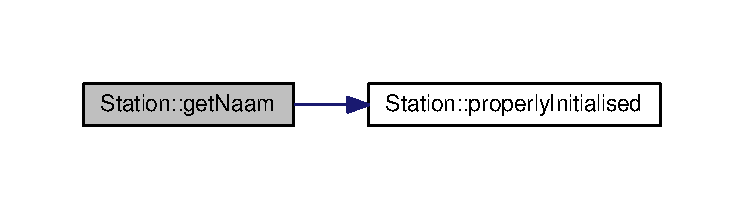
\includegraphics[width=338pt]{class_station_a6d4234bcd1027dc83c7984e207e8bd74_cgraph}
\end{center}
\end{figure}




Here is the caller graph for this function\+:
\nopagebreak
\begin{figure}[H]
\begin{center}
\leavevmode
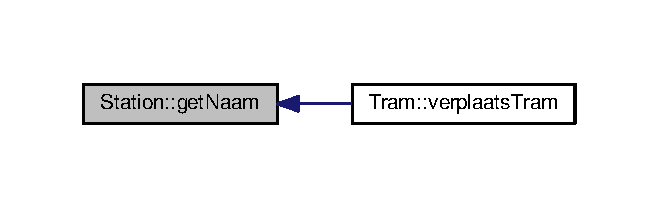
\includegraphics[width=316pt]{class_station_a6d4234bcd1027dc83c7984e207e8bd74_icgraph}
\end{center}
\end{figure}


\index{Station@{Station}!get\+Spoor@{get\+Spoor}}
\index{get\+Spoor@{get\+Spoor}!Station@{Station}}
\subsubsection[{\texorpdfstring{get\+Spoor() const }{getSpoor() const }}]{\setlength{\rightskip}{0pt plus 5cm}{\bf Spoor} $\ast$ Station\+::get\+Spoor (
\begin{DoxyParamCaption}
{}
\end{DoxyParamCaption}
) const}\hypertarget{class_station_af7ea9d2ec05b56832c0e1a2fe2303ee1}{}\label{class_station_af7ea9d2ec05b56832c0e1a2fe2303ee1}


Geef het \hyperlink{class_spoor}{Spoor} terug. 

\begin{DoxyReturn}{Returns}
Het spoor. R\+E\+Q\+U\+I\+RE(this-\/$>$\hyperlink{class_station_a5749af84d13b71d34aa1fb5b0a935a20}{properly\+Initialised()}, \char`\"{}\+Station was niet geinitialiseerd bij de aanroep van get\+Spoor.\char`\"{});~\newline

\end{DoxyReturn}


Here is the call graph for this function\+:
\nopagebreak
\begin{figure}[H]
\begin{center}
\leavevmode
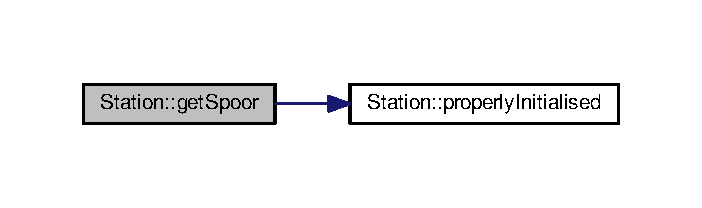
\includegraphics[width=337pt]{class_station_af7ea9d2ec05b56832c0e1a2fe2303ee1_cgraph}
\end{center}
\end{figure}


\index{Station@{Station}!get\+Volgende@{get\+Volgende}}
\index{get\+Volgende@{get\+Volgende}!Station@{Station}}
\subsubsection[{\texorpdfstring{get\+Volgende() const }{getVolgende() const }}]{\setlength{\rightskip}{0pt plus 5cm}{\bf Station} $\ast$ Station\+::get\+Volgende (
\begin{DoxyParamCaption}
{}
\end{DoxyParamCaption}
) const}\hypertarget{class_station_a2c81d14029f13b972c015a16813c8d34}{}\label{class_station_a2c81d14029f13b972c015a16813c8d34}


Geef het volgende station. 

\begin{DoxyReturn}{Returns}
Het volgende station.
\end{DoxyReturn}
R\+E\+Q\+U\+I\+RE(this-\/$>$\hyperlink{class_station_a5749af84d13b71d34aa1fb5b0a935a20}{properly\+Initialised()}, \char`\"{}\+Station was niet geinitialiseerd bij de aanroep van get\+Volgende.\char`\"{});~\newline


Here is the call graph for this function\+:
\nopagebreak
\begin{figure}[H]
\begin{center}
\leavevmode
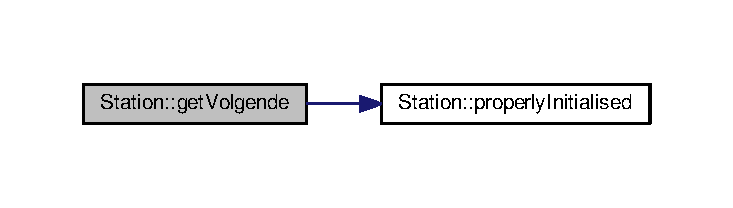
\includegraphics[width=350pt]{class_station_a2c81d14029f13b972c015a16813c8d34_cgraph}
\end{center}
\end{figure}


\index{Station@{Station}!get\+Vorige@{get\+Vorige}}
\index{get\+Vorige@{get\+Vorige}!Station@{Station}}
\subsubsection[{\texorpdfstring{get\+Vorige() const }{getVorige() const }}]{\setlength{\rightskip}{0pt plus 5cm}{\bf Station} $\ast$ Station\+::get\+Vorige (
\begin{DoxyParamCaption}
{}
\end{DoxyParamCaption}
) const}\hypertarget{class_station_a2adced993339721e8731bfa55762f4f9}{}\label{class_station_a2adced993339721e8731bfa55762f4f9}


Geef het vorig station terug. 

\begin{DoxyReturn}{Returns}
Het vorig station.
\end{DoxyReturn}
R\+E\+Q\+U\+I\+RE(this-\/$>$\hyperlink{class_station_a5749af84d13b71d34aa1fb5b0a935a20}{properly\+Initialised()}, \char`\"{}\+Station was niet geinitialiseerd bij de aanroep van get\+Vorige.\char`\"{});~\newline


Here is the call graph for this function\+:
\nopagebreak
\begin{figure}[H]
\begin{center}
\leavevmode
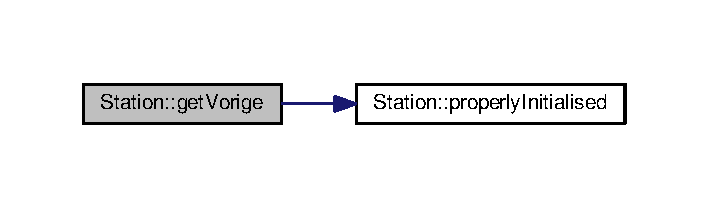
\includegraphics[width=340pt]{class_station_a2adced993339721e8731bfa55762f4f9_cgraph}
\end{center}
\end{figure}


\index{Station@{Station}!properly\+Initialised@{properly\+Initialised}}
\index{properly\+Initialised@{properly\+Initialised}!Station@{Station}}
\subsubsection[{\texorpdfstring{properly\+Initialised() const }{properlyInitialised() const }}]{\setlength{\rightskip}{0pt plus 5cm}bool Station\+::properly\+Initialised (
\begin{DoxyParamCaption}
{}
\end{DoxyParamCaption}
) const}\hypertarget{class_station_a5749af84d13b71d34aa1fb5b0a935a20}{}\label{class_station_a5749af84d13b71d34aa1fb5b0a935a20}


Kijk na of de constructor in de juiste staat geeindigd is. 

\begin{DoxyReturn}{Returns}
Boolean die aangeeft of het object juist geinitialiseerd is. 
\end{DoxyReturn}


Here is the caller graph for this function\+:
\nopagebreak
\begin{figure}[H]
\begin{center}
\leavevmode
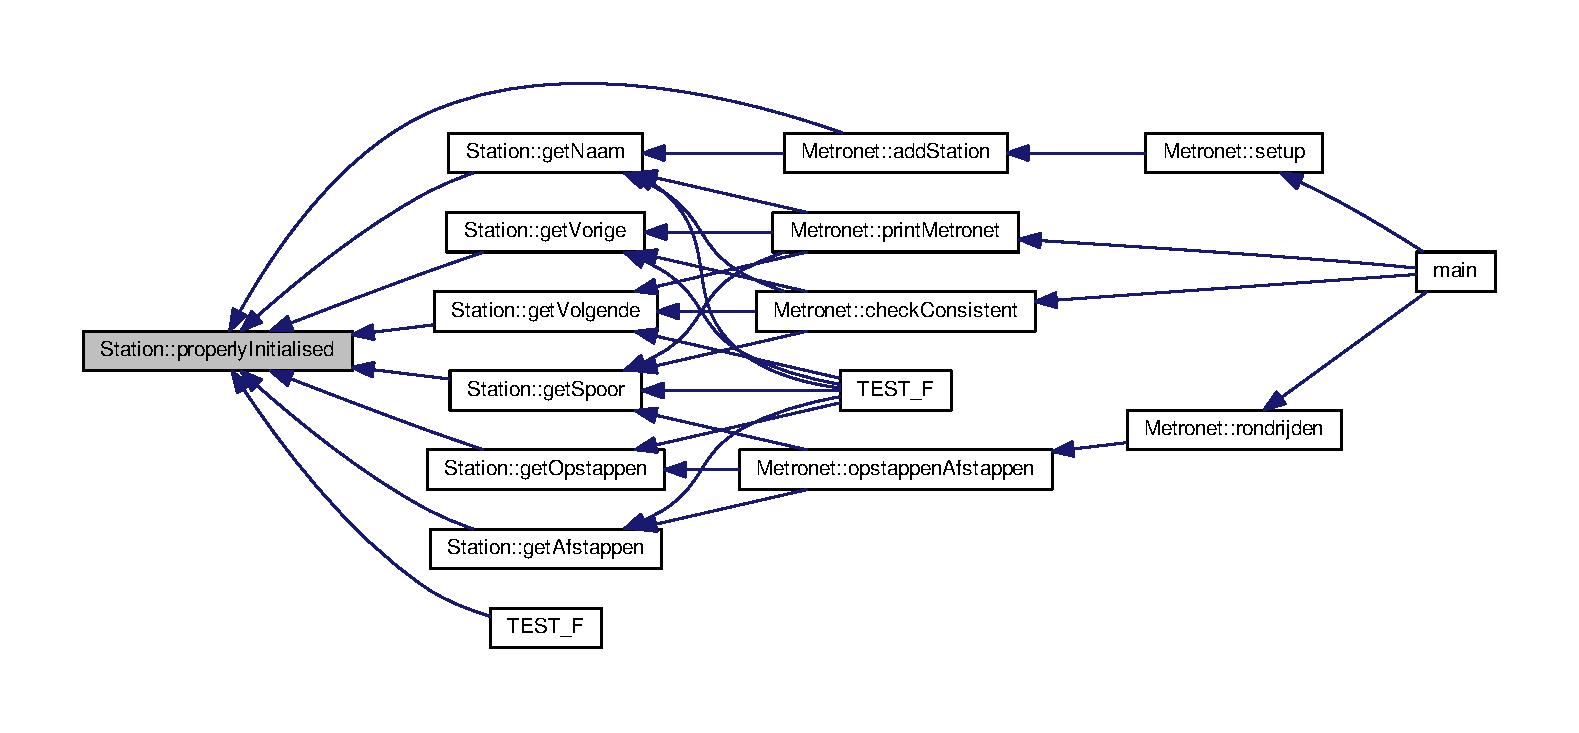
\includegraphics[width=350pt]{class_station_a5749af84d13b71d34aa1fb5b0a935a20_icgraph}
\end{center}
\end{figure}




The documentation for this class was generated from the following files\+:\begin{DoxyCompactItemize}
\item 
/home/jonathan/\+Desktop/\+Project Software Engineering/\+Metronet/\+P\+S\+E/src/\hyperlink{_station_8h}{Station.\+h}\item 
/home/jonathan/\+Desktop/\+Project Software Engineering/\+Metronet/\+P\+S\+E/src/\hyperlink{_station_8cpp}{Station.\+cpp}\end{DoxyCompactItemize}

\hypertarget{class_ti_xml_attribute}{}\section{Ti\+Xml\+Attribute Class Reference}
\label{class_ti_xml_attribute}\index{Ti\+Xml\+Attribute@{Ti\+Xml\+Attribute}}


{\ttfamily \#include $<$tinyxml.\+h$>$}



Inheritance diagram for Ti\+Xml\+Attribute\+:
\nopagebreak
\begin{figure}[H]
\begin{center}
\leavevmode
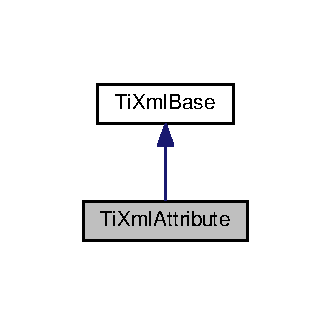
\includegraphics[width=159pt]{class_ti_xml_attribute__inherit__graph}
\end{center}
\end{figure}


Collaboration diagram for Ti\+Xml\+Attribute\+:
\nopagebreak
\begin{figure}[H]
\begin{center}
\leavevmode
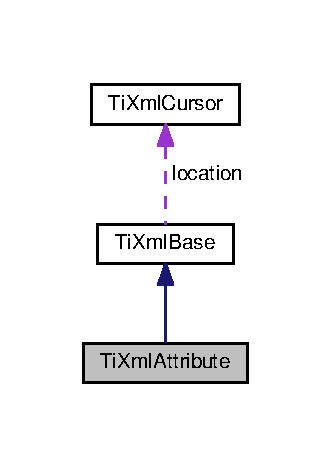
\includegraphics[width=159pt]{class_ti_xml_attribute__coll__graph}
\end{center}
\end{figure}
\subsection*{Public Member Functions}
\begin{DoxyCompactItemize}
\item 
\hyperlink{class_ti_xml_attribute_a9cfa3c8179873fd485d83003b114f8e1}{Ti\+Xml\+Attribute} ()
\begin{DoxyCompactList}\small\item\em Construct an empty attribute. \end{DoxyCompactList}\item 
\hyperlink{class_ti_xml_attribute_a759d0b76fb8fcf765ecab243bc14f05e}{Ti\+Xml\+Attribute} (const char $\ast$\+\_\+name, const char $\ast$\+\_\+value)
\begin{DoxyCompactList}\small\item\em Construct an attribute with a name and value. \end{DoxyCompactList}\item 
const char $\ast$ \hyperlink{class_ti_xml_attribute_a298a57287d305904ba6bd96ae6f78d3d}{Name} () const 
\begin{DoxyCompactList}\small\item\em Return the name of this attribute. \end{DoxyCompactList}\item 
const char $\ast$ \hyperlink{class_ti_xml_attribute_a0f874490eac8ca00ee0070765d0e97e3}{Value} () const 
\begin{DoxyCompactList}\small\item\em Return the value of this attribute. \end{DoxyCompactList}\item 
int \hyperlink{class_ti_xml_attribute_aa1a20ad59dc7e89a0ab265396360d50f}{Int\+Value} () const 
\begin{DoxyCompactList}\small\item\em Return the value of this attribute, converted to an integer. \end{DoxyCompactList}\item 
double \hyperlink{class_ti_xml_attribute_a2880ddef53fc7522c99535273954d230}{Double\+Value} () const 
\begin{DoxyCompactList}\small\item\em Return the value of this attribute, converted to a double. \end{DoxyCompactList}\item 
const \hyperlink{tinyxml_8h_a92bada05fd84d9a0c9a5bbe53de26887}{T\+I\+X\+M\+L\+\_\+\+S\+T\+R\+I\+NG} \& \hyperlink{class_ti_xml_attribute_a64cee17bceb8232eb0736d26dd082d79}{Name\+T\+Str} () const 
\item 
int \hyperlink{class_ti_xml_attribute_ad6c93088ee21af41a107931223339344}{Query\+Int\+Value} (int $\ast$\+\_\+value) const 
\item 
int \hyperlink{class_ti_xml_attribute_ac87b2a8489906a5d7aa2875f20be3513}{Query\+Double\+Value} (double $\ast$\+\_\+value) const 
\begin{DoxyCompactList}\small\item\em Query\+Double\+Value examines the value string. See \hyperlink{class_ti_xml_attribute_ad6c93088ee21af41a107931223339344}{Query\+Int\+Value()}. \end{DoxyCompactList}\item 
void \hyperlink{class_ti_xml_attribute_ab7fa3d21ff8d7c5764cf9af15b667a99}{Set\+Name} (const char $\ast$\+\_\+name)
\begin{DoxyCompactList}\small\item\em Set the name of this attribute. \end{DoxyCompactList}\item 
void \hyperlink{class_ti_xml_attribute_a2dae44178f668b3cb48101be4f2236a0}{Set\+Value} (const char $\ast$\+\_\+value)
\begin{DoxyCompactList}\small\item\em Set the value. \end{DoxyCompactList}\item 
void \hyperlink{class_ti_xml_attribute_a7e065df640116a62ea4f4b7da5449cc8}{Set\+Int\+Value} (int \+\_\+value)
\begin{DoxyCompactList}\small\item\em Set the value from an integer. \end{DoxyCompactList}\item 
void \hyperlink{class_ti_xml_attribute_a0316da31373496c4368ad549bf711394}{Set\+Double\+Value} (double \+\_\+value)
\begin{DoxyCompactList}\small\item\em Set the value from a double. \end{DoxyCompactList}\item 
const \hyperlink{class_ti_xml_attribute}{Ti\+Xml\+Attribute} $\ast$ \hyperlink{class_ti_xml_attribute_a776478980776a024f7c2846eec640f65}{Next} () const 
\begin{DoxyCompactList}\small\item\em Get the next sibling attribute in the D\+OM. Returns null at end. \end{DoxyCompactList}\item 
\hyperlink{class_ti_xml_attribute}{Ti\+Xml\+Attribute} $\ast$ \hyperlink{class_ti_xml_attribute_a138320aa7793b148ba7e5bd0a0ea4db6}{Next} ()
\item 
const \hyperlink{class_ti_xml_attribute}{Ti\+Xml\+Attribute} $\ast$ \hyperlink{class_ti_xml_attribute_a54a5f8730c7b02b9a41b74e12e27fe86}{Previous} () const 
\begin{DoxyCompactList}\small\item\em Get the previous sibling attribute in the D\+OM. Returns null at beginning. \end{DoxyCompactList}\item 
\hyperlink{class_ti_xml_attribute}{Ti\+Xml\+Attribute} $\ast$ \hyperlink{class_ti_xml_attribute_ae4dabc932cba945ed1e92fec5f121193}{Previous} ()
\item 
bool \hyperlink{class_ti_xml_attribute_ae48c2a65b520d453914ce4e845d607cf}{operator==} (const \hyperlink{class_ti_xml_attribute}{Ti\+Xml\+Attribute} \&rhs) const 
\item 
bool \hyperlink{class_ti_xml_attribute_adb8b6f2cad5948e73e383182e7ce10de}{operator$<$} (const \hyperlink{class_ti_xml_attribute}{Ti\+Xml\+Attribute} \&rhs) const 
\item 
bool \hyperlink{class_ti_xml_attribute_a867562769ef9778c1690cd373246b05b}{operator$>$} (const \hyperlink{class_ti_xml_attribute}{Ti\+Xml\+Attribute} \&rhs) const 
\item 
virtual const char $\ast$ \hyperlink{class_ti_xml_attribute_ad62774421b814894b995af3b5d231dda}{Parse} (const char $\ast$p, \hyperlink{class_ti_xml_parsing_data}{Ti\+Xml\+Parsing\+Data} $\ast$data, \hyperlink{tinyxml_8h_a88d51847a13ee0f4b4d320d03d2c4d96}{Ti\+Xml\+Encoding} encoding)
\item 
virtual void \hyperlink{class_ti_xml_attribute_acc04956c1d5c4c31fe74f7a7528d109a}{Print} (F\+I\+LE $\ast$cfile, int depth) const 
\item 
void \hyperlink{class_ti_xml_attribute_a19e6b6862a80b188571c47947e88d030}{Print} (F\+I\+LE $\ast$cfile, int depth, \hyperlink{tinyxml_8h_a92bada05fd84d9a0c9a5bbe53de26887}{T\+I\+X\+M\+L\+\_\+\+S\+T\+R\+I\+NG} $\ast$str) const 
\item 
void \hyperlink{class_ti_xml_attribute_ac12a94d4548302afb12f488ba101f7d1}{Set\+Document} (\hyperlink{class_ti_xml_document}{Ti\+Xml\+Document} $\ast$doc)
\end{DoxyCompactItemize}
\subsection*{Friends}
\begin{DoxyCompactItemize}
\item 
class \hyperlink{class_ti_xml_attribute_a35a7b7f89f708527677d5078d41ce0bf}{Ti\+Xml\+Attribute\+Set}
\end{DoxyCompactItemize}
\subsection*{Additional Inherited Members}


\subsection{Detailed Description}
An attribute is a name-\/value pair. Elements have an arbitrary number of attributes, each with a unique name.

\begin{DoxyNote}{Note}
The attributes are not Ti\+Xml\+Nodes, since they are not part of the tiny\+X\+ML document object model. There are other suggested ways to look at this problem. 
\end{DoxyNote}


\subsection{Constructor \& Destructor Documentation}
\index{Ti\+Xml\+Attribute@{Ti\+Xml\+Attribute}!Ti\+Xml\+Attribute@{Ti\+Xml\+Attribute}}
\index{Ti\+Xml\+Attribute@{Ti\+Xml\+Attribute}!Ti\+Xml\+Attribute@{Ti\+Xml\+Attribute}}
\subsubsection[{\texorpdfstring{Ti\+Xml\+Attribute()}{TiXmlAttribute()}}]{\setlength{\rightskip}{0pt plus 5cm}Ti\+Xml\+Attribute\+::\+Ti\+Xml\+Attribute (
\begin{DoxyParamCaption}
{}
\end{DoxyParamCaption}
)\hspace{0.3cm}{\ttfamily [inline]}}\hypertarget{class_ti_xml_attribute_a9cfa3c8179873fd485d83003b114f8e1}{}\label{class_ti_xml_attribute_a9cfa3c8179873fd485d83003b114f8e1}


Construct an empty attribute. 

\index{Ti\+Xml\+Attribute@{Ti\+Xml\+Attribute}!Ti\+Xml\+Attribute@{Ti\+Xml\+Attribute}}
\index{Ti\+Xml\+Attribute@{Ti\+Xml\+Attribute}!Ti\+Xml\+Attribute@{Ti\+Xml\+Attribute}}
\subsubsection[{\texorpdfstring{Ti\+Xml\+Attribute(const char $\ast$\+\_\+name, const char $\ast$\+\_\+value)}{TiXmlAttribute(const char *_name, const char *_value)}}]{\setlength{\rightskip}{0pt plus 5cm}Ti\+Xml\+Attribute\+::\+Ti\+Xml\+Attribute (
\begin{DoxyParamCaption}
\item[{const char $\ast$}]{\+\_\+name, }
\item[{const char $\ast$}]{\+\_\+value}
\end{DoxyParamCaption}
)\hspace{0.3cm}{\ttfamily [inline]}}\hypertarget{class_ti_xml_attribute_a759d0b76fb8fcf765ecab243bc14f05e}{}\label{class_ti_xml_attribute_a759d0b76fb8fcf765ecab243bc14f05e}


Construct an attribute with a name and value. 



\subsection{Member Function Documentation}
\index{Ti\+Xml\+Attribute@{Ti\+Xml\+Attribute}!Double\+Value@{Double\+Value}}
\index{Double\+Value@{Double\+Value}!Ti\+Xml\+Attribute@{Ti\+Xml\+Attribute}}
\subsubsection[{\texorpdfstring{Double\+Value() const }{DoubleValue() const }}]{\setlength{\rightskip}{0pt plus 5cm}double Ti\+Xml\+Attribute\+::\+Double\+Value (
\begin{DoxyParamCaption}
{}
\end{DoxyParamCaption}
) const}\hypertarget{class_ti_xml_attribute_a2880ddef53fc7522c99535273954d230}{}\label{class_ti_xml_attribute_a2880ddef53fc7522c99535273954d230}


Return the value of this attribute, converted to a double. 

\index{Ti\+Xml\+Attribute@{Ti\+Xml\+Attribute}!Int\+Value@{Int\+Value}}
\index{Int\+Value@{Int\+Value}!Ti\+Xml\+Attribute@{Ti\+Xml\+Attribute}}
\subsubsection[{\texorpdfstring{Int\+Value() const }{IntValue() const }}]{\setlength{\rightskip}{0pt plus 5cm}int Ti\+Xml\+Attribute\+::\+Int\+Value (
\begin{DoxyParamCaption}
{}
\end{DoxyParamCaption}
) const}\hypertarget{class_ti_xml_attribute_aa1a20ad59dc7e89a0ab265396360d50f}{}\label{class_ti_xml_attribute_aa1a20ad59dc7e89a0ab265396360d50f}


Return the value of this attribute, converted to an integer. 

\index{Ti\+Xml\+Attribute@{Ti\+Xml\+Attribute}!Name@{Name}}
\index{Name@{Name}!Ti\+Xml\+Attribute@{Ti\+Xml\+Attribute}}
\subsubsection[{\texorpdfstring{Name() const }{Name() const }}]{\setlength{\rightskip}{0pt plus 5cm}const char$\ast$ Ti\+Xml\+Attribute\+::\+Name (
\begin{DoxyParamCaption}
{}
\end{DoxyParamCaption}
) const\hspace{0.3cm}{\ttfamily [inline]}}\hypertarget{class_ti_xml_attribute_a298a57287d305904ba6bd96ae6f78d3d}{}\label{class_ti_xml_attribute_a298a57287d305904ba6bd96ae6f78d3d}


Return the name of this attribute. 



Here is the caller graph for this function\+:
\nopagebreak
\begin{figure}[H]
\begin{center}
\leavevmode
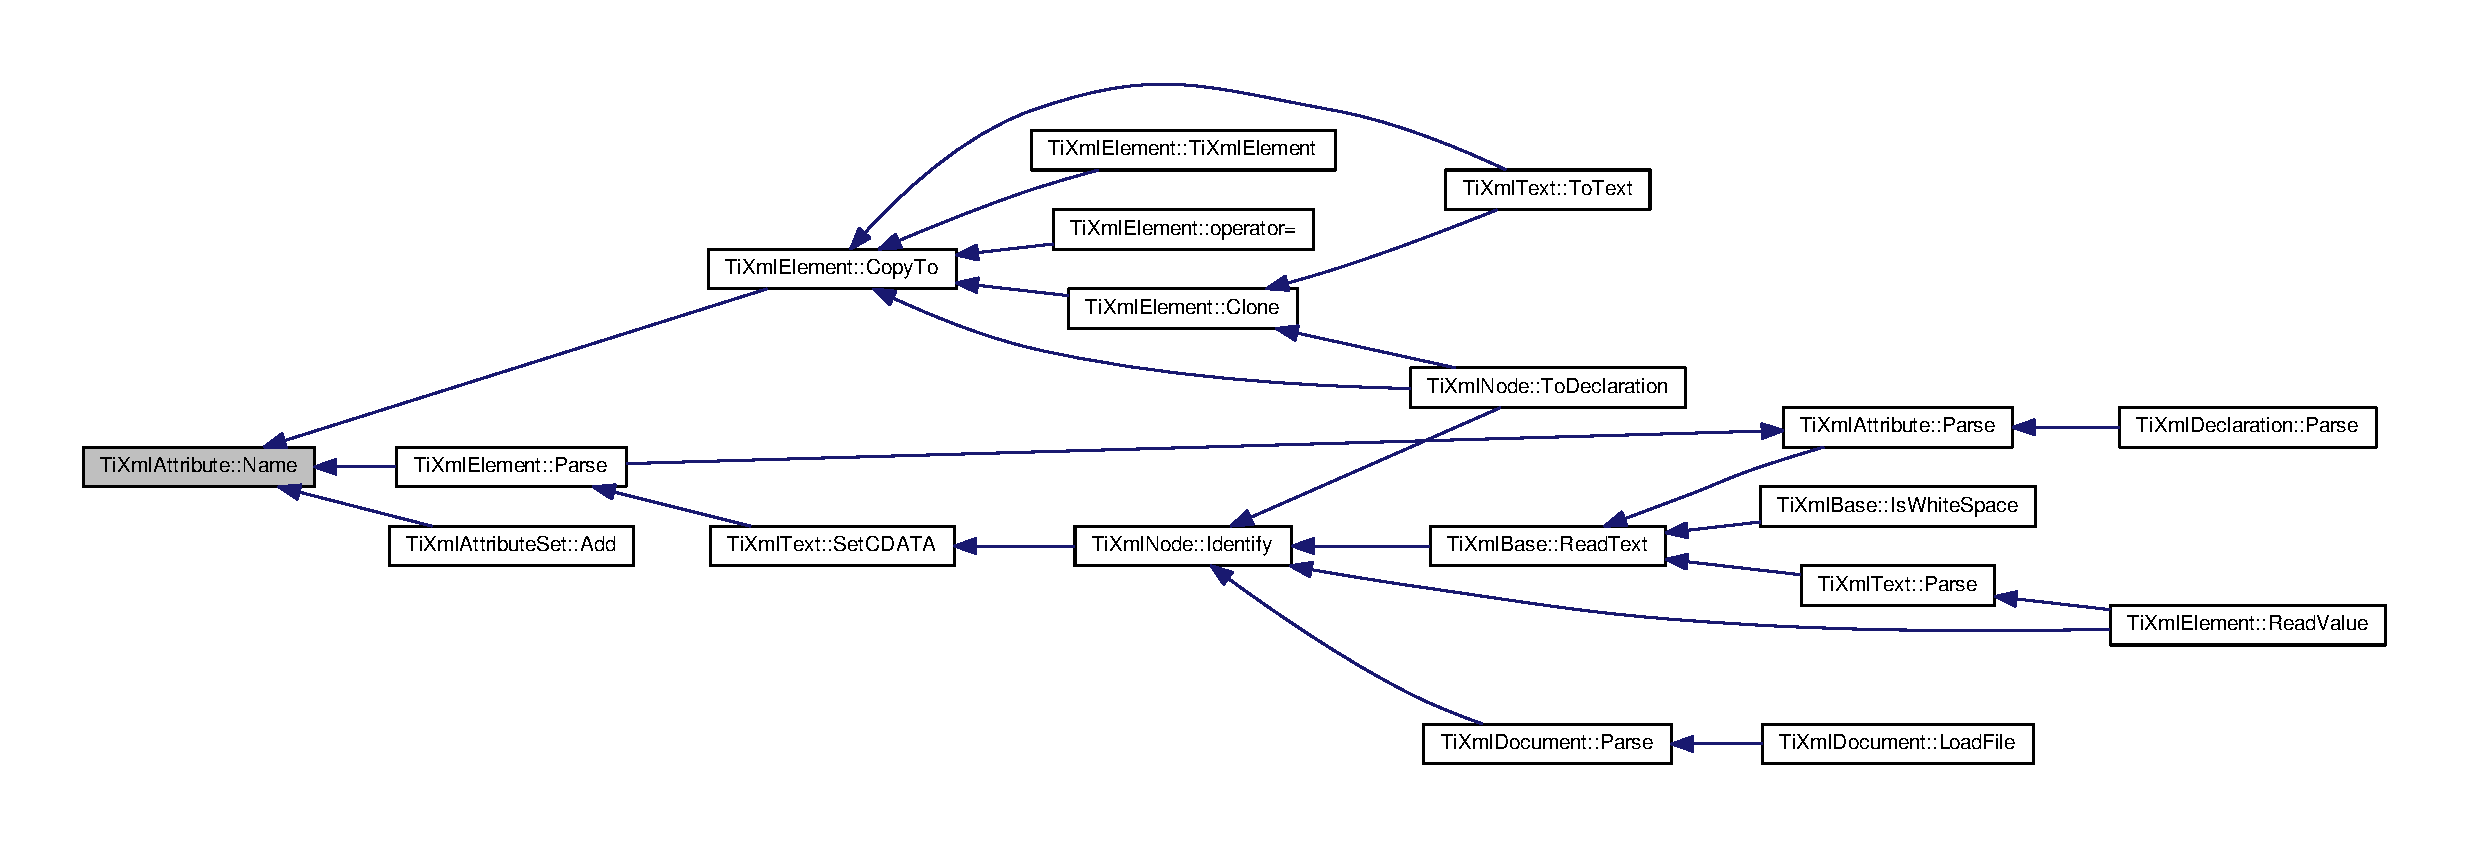
\includegraphics[width=350pt]{class_ti_xml_attribute_a298a57287d305904ba6bd96ae6f78d3d_icgraph}
\end{center}
\end{figure}


\index{Ti\+Xml\+Attribute@{Ti\+Xml\+Attribute}!Name\+T\+Str@{Name\+T\+Str}}
\index{Name\+T\+Str@{Name\+T\+Str}!Ti\+Xml\+Attribute@{Ti\+Xml\+Attribute}}
\subsubsection[{\texorpdfstring{Name\+T\+Str() const }{NameTStr() const }}]{\setlength{\rightskip}{0pt plus 5cm}const {\bf T\+I\+X\+M\+L\+\_\+\+S\+T\+R\+I\+NG}\& Ti\+Xml\+Attribute\+::\+Name\+T\+Str (
\begin{DoxyParamCaption}
{}
\end{DoxyParamCaption}
) const\hspace{0.3cm}{\ttfamily [inline]}}\hypertarget{class_ti_xml_attribute_a64cee17bceb8232eb0736d26dd082d79}{}\label{class_ti_xml_attribute_a64cee17bceb8232eb0736d26dd082d79}


Here is the caller graph for this function\+:
\nopagebreak
\begin{figure}[H]
\begin{center}
\leavevmode
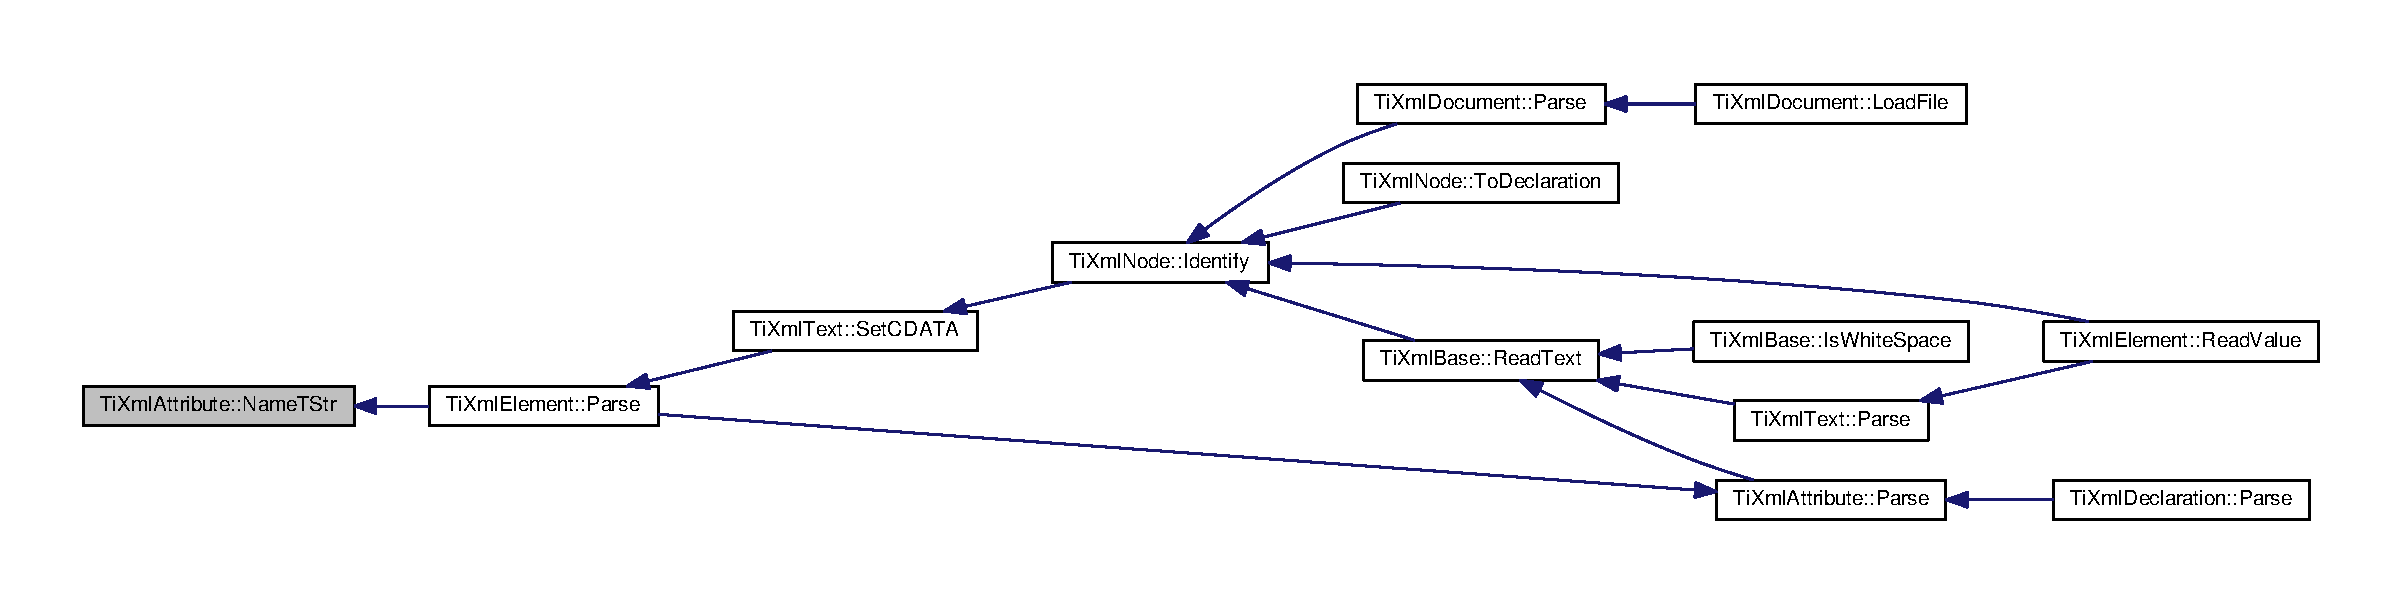
\includegraphics[width=350pt]{class_ti_xml_attribute_a64cee17bceb8232eb0736d26dd082d79_icgraph}
\end{center}
\end{figure}


\index{Ti\+Xml\+Attribute@{Ti\+Xml\+Attribute}!Next@{Next}}
\index{Next@{Next}!Ti\+Xml\+Attribute@{Ti\+Xml\+Attribute}}
\subsubsection[{\texorpdfstring{Next() const }{Next() const }}]{\setlength{\rightskip}{0pt plus 5cm}const {\bf Ti\+Xml\+Attribute} $\ast$ Ti\+Xml\+Attribute\+::\+Next (
\begin{DoxyParamCaption}
{}
\end{DoxyParamCaption}
) const}\hypertarget{class_ti_xml_attribute_a776478980776a024f7c2846eec640f65}{}\label{class_ti_xml_attribute_a776478980776a024f7c2846eec640f65}


Get the next sibling attribute in the D\+OM. Returns null at end. 



Here is the caller graph for this function\+:
\nopagebreak
\begin{figure}[H]
\begin{center}
\leavevmode
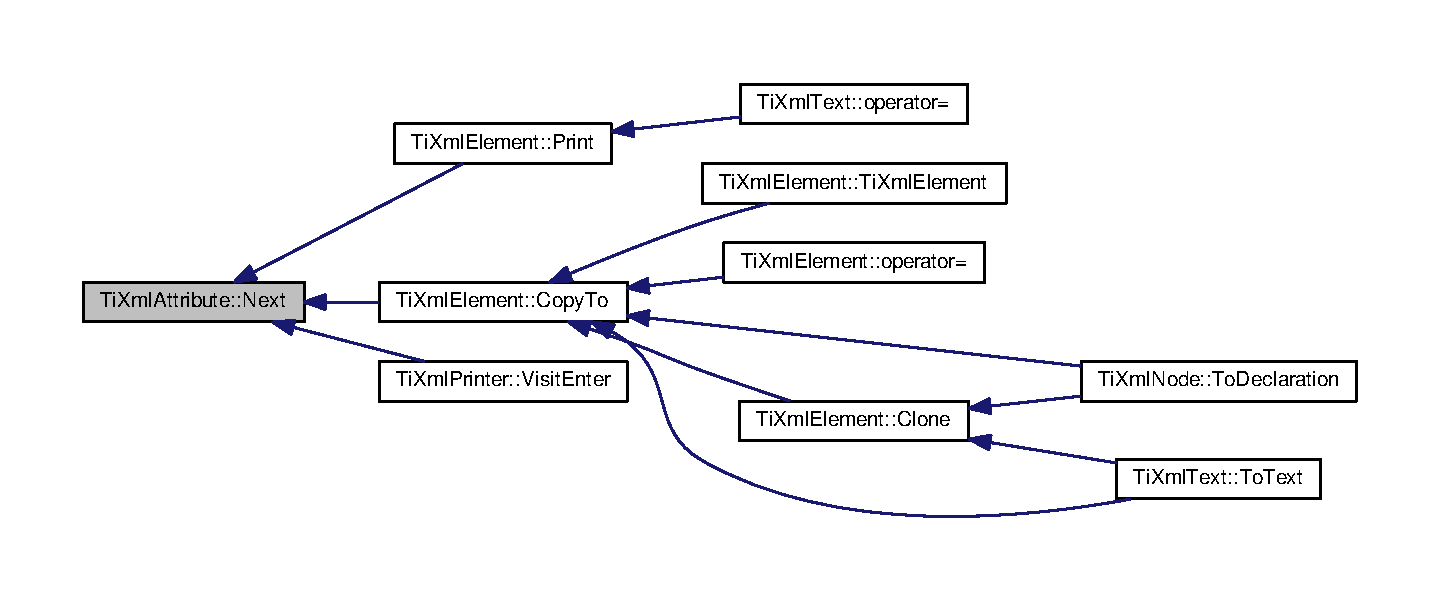
\includegraphics[width=350pt]{class_ti_xml_attribute_a776478980776a024f7c2846eec640f65_icgraph}
\end{center}
\end{figure}


\index{Ti\+Xml\+Attribute@{Ti\+Xml\+Attribute}!Next@{Next}}
\index{Next@{Next}!Ti\+Xml\+Attribute@{Ti\+Xml\+Attribute}}
\subsubsection[{\texorpdfstring{Next()}{Next()}}]{\setlength{\rightskip}{0pt plus 5cm}{\bf Ti\+Xml\+Attribute}$\ast$ Ti\+Xml\+Attribute\+::\+Next (
\begin{DoxyParamCaption}
{}
\end{DoxyParamCaption}
)\hspace{0.3cm}{\ttfamily [inline]}}\hypertarget{class_ti_xml_attribute_a138320aa7793b148ba7e5bd0a0ea4db6}{}\label{class_ti_xml_attribute_a138320aa7793b148ba7e5bd0a0ea4db6}
\index{Ti\+Xml\+Attribute@{Ti\+Xml\+Attribute}!operator$<$@{operator$<$}}
\index{operator$<$@{operator$<$}!Ti\+Xml\+Attribute@{Ti\+Xml\+Attribute}}
\subsubsection[{\texorpdfstring{operator$<$(const Ti\+Xml\+Attribute \&rhs) const }{operator<(const TiXmlAttribute &rhs) const }}]{\setlength{\rightskip}{0pt plus 5cm}bool Ti\+Xml\+Attribute\+::operator$<$ (
\begin{DoxyParamCaption}
\item[{const {\bf Ti\+Xml\+Attribute} \&}]{rhs}
\end{DoxyParamCaption}
) const\hspace{0.3cm}{\ttfamily [inline]}}\hypertarget{class_ti_xml_attribute_adb8b6f2cad5948e73e383182e7ce10de}{}\label{class_ti_xml_attribute_adb8b6f2cad5948e73e383182e7ce10de}
\index{Ti\+Xml\+Attribute@{Ti\+Xml\+Attribute}!operator==@{operator==}}
\index{operator==@{operator==}!Ti\+Xml\+Attribute@{Ti\+Xml\+Attribute}}
\subsubsection[{\texorpdfstring{operator==(const Ti\+Xml\+Attribute \&rhs) const }{operator==(const TiXmlAttribute &rhs) const }}]{\setlength{\rightskip}{0pt plus 5cm}bool Ti\+Xml\+Attribute\+::operator== (
\begin{DoxyParamCaption}
\item[{const {\bf Ti\+Xml\+Attribute} \&}]{rhs}
\end{DoxyParamCaption}
) const\hspace{0.3cm}{\ttfamily [inline]}}\hypertarget{class_ti_xml_attribute_ae48c2a65b520d453914ce4e845d607cf}{}\label{class_ti_xml_attribute_ae48c2a65b520d453914ce4e845d607cf}
\index{Ti\+Xml\+Attribute@{Ti\+Xml\+Attribute}!operator$>$@{operator$>$}}
\index{operator$>$@{operator$>$}!Ti\+Xml\+Attribute@{Ti\+Xml\+Attribute}}
\subsubsection[{\texorpdfstring{operator$>$(const Ti\+Xml\+Attribute \&rhs) const }{operator>(const TiXmlAttribute &rhs) const }}]{\setlength{\rightskip}{0pt plus 5cm}bool Ti\+Xml\+Attribute\+::operator$>$ (
\begin{DoxyParamCaption}
\item[{const {\bf Ti\+Xml\+Attribute} \&}]{rhs}
\end{DoxyParamCaption}
) const\hspace{0.3cm}{\ttfamily [inline]}}\hypertarget{class_ti_xml_attribute_a867562769ef9778c1690cd373246b05b}{}\label{class_ti_xml_attribute_a867562769ef9778c1690cd373246b05b}
\index{Ti\+Xml\+Attribute@{Ti\+Xml\+Attribute}!Parse@{Parse}}
\index{Parse@{Parse}!Ti\+Xml\+Attribute@{Ti\+Xml\+Attribute}}
\subsubsection[{\texorpdfstring{Parse(const char $\ast$p, Ti\+Xml\+Parsing\+Data $\ast$data, Ti\+Xml\+Encoding encoding)}{Parse(const char *p, TiXmlParsingData *data, TiXmlEncoding encoding)}}]{\setlength{\rightskip}{0pt plus 5cm}const char $\ast$ Ti\+Xml\+Attribute\+::\+Parse (
\begin{DoxyParamCaption}
\item[{const char $\ast$}]{p, }
\item[{{\bf Ti\+Xml\+Parsing\+Data} $\ast$}]{data, }
\item[{{\bf Ti\+Xml\+Encoding}}]{encoding}
\end{DoxyParamCaption}
)\hspace{0.3cm}{\ttfamily [virtual]}}\hypertarget{class_ti_xml_attribute_ad62774421b814894b995af3b5d231dda}{}\label{class_ti_xml_attribute_ad62774421b814894b995af3b5d231dda}


Implements \hyperlink{class_ti_xml_base_a00e4edb0219d00a1379c856e5a1d2025}{Ti\+Xml\+Base}.



Here is the call graph for this function\+:
\nopagebreak
\begin{figure}[H]
\begin{center}
\leavevmode
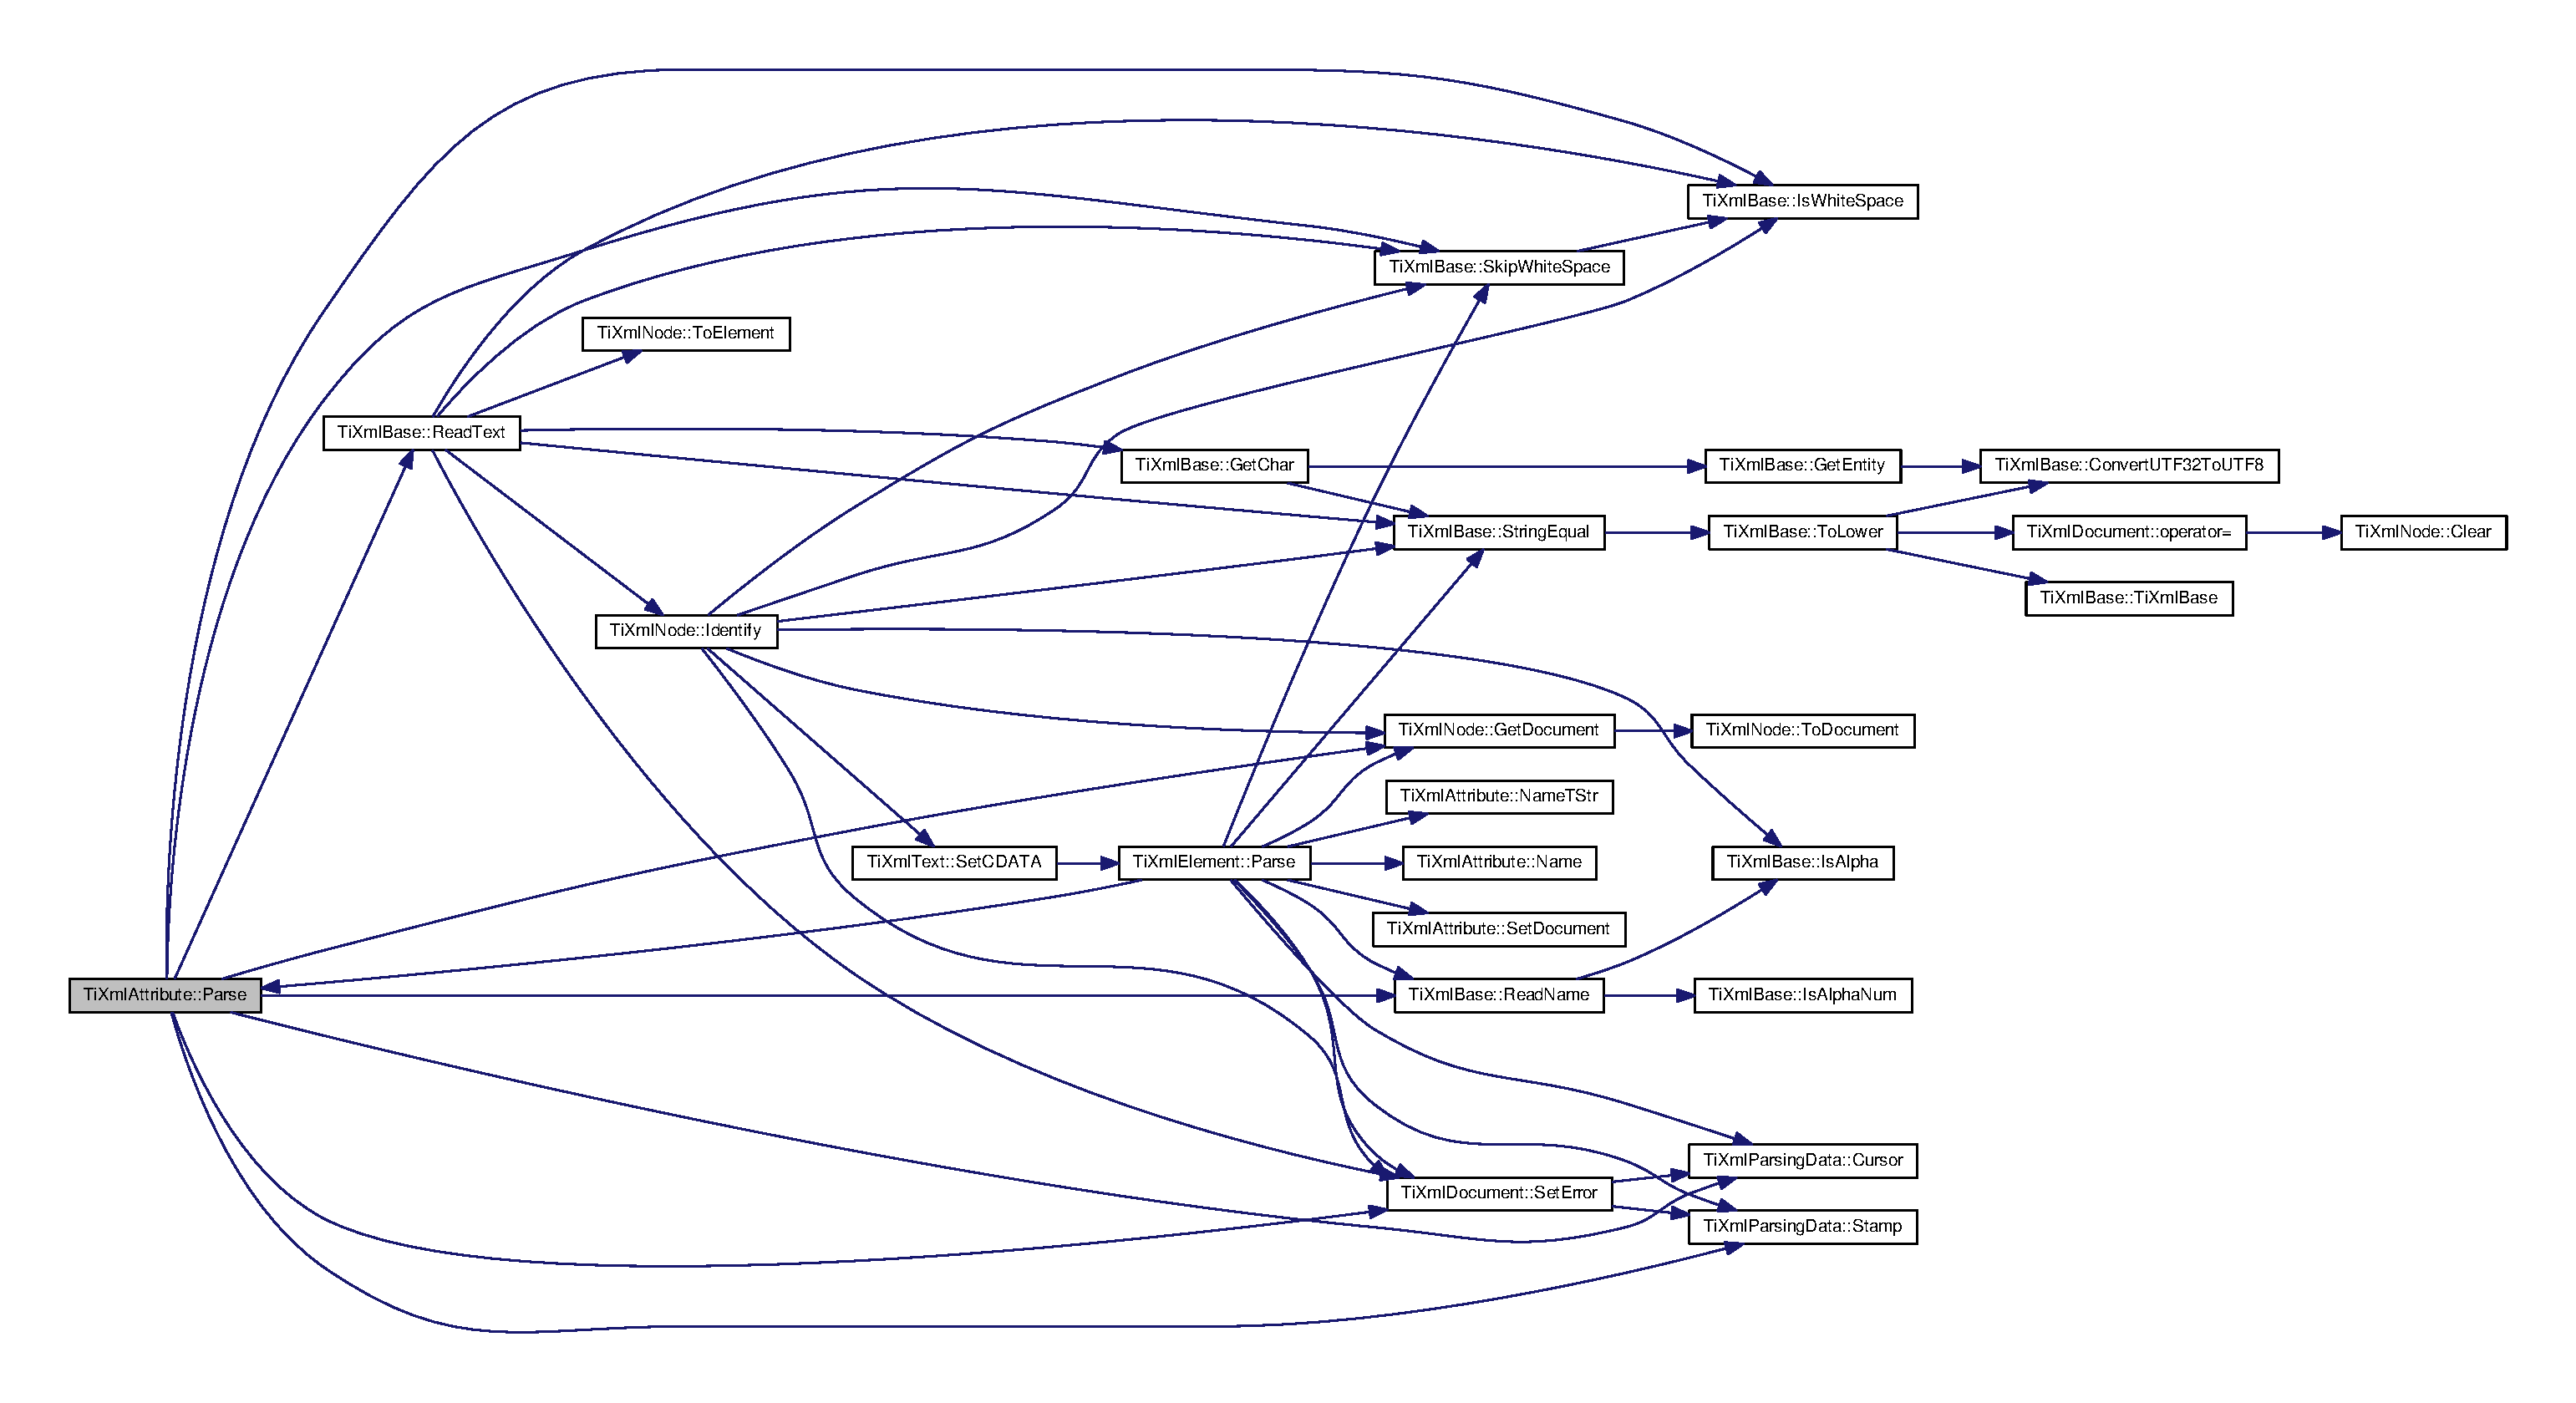
\includegraphics[width=350pt]{class_ti_xml_attribute_ad62774421b814894b995af3b5d231dda_cgraph}
\end{center}
\end{figure}




Here is the caller graph for this function\+:
\nopagebreak
\begin{figure}[H]
\begin{center}
\leavevmode
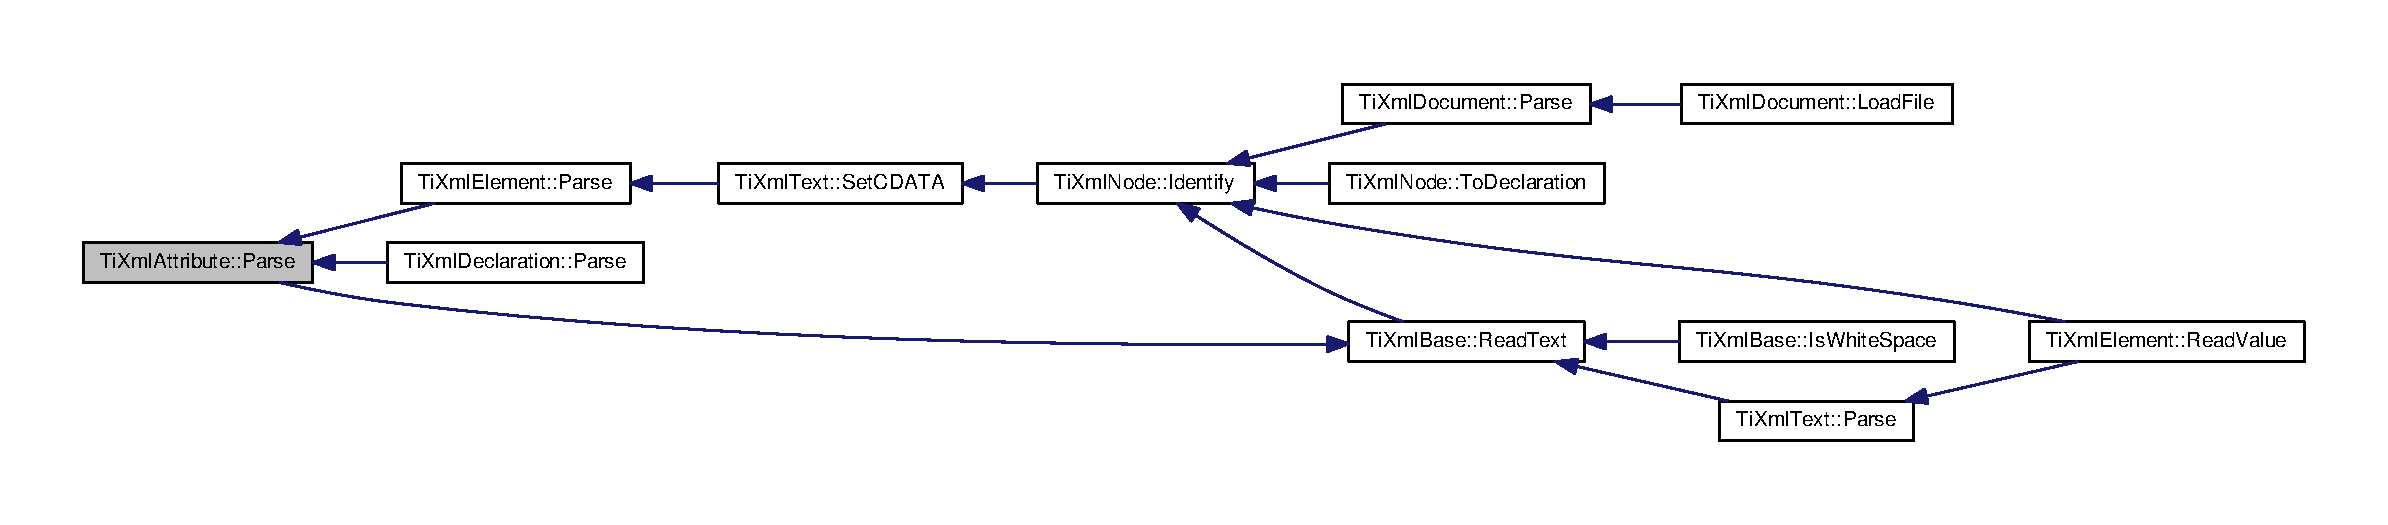
\includegraphics[width=350pt]{class_ti_xml_attribute_ad62774421b814894b995af3b5d231dda_icgraph}
\end{center}
\end{figure}


\index{Ti\+Xml\+Attribute@{Ti\+Xml\+Attribute}!Previous@{Previous}}
\index{Previous@{Previous}!Ti\+Xml\+Attribute@{Ti\+Xml\+Attribute}}
\subsubsection[{\texorpdfstring{Previous() const }{Previous() const }}]{\setlength{\rightskip}{0pt plus 5cm}const {\bf Ti\+Xml\+Attribute} $\ast$ Ti\+Xml\+Attribute\+::\+Previous (
\begin{DoxyParamCaption}
{}
\end{DoxyParamCaption}
) const}\hypertarget{class_ti_xml_attribute_a54a5f8730c7b02b9a41b74e12e27fe86}{}\label{class_ti_xml_attribute_a54a5f8730c7b02b9a41b74e12e27fe86}


Get the previous sibling attribute in the D\+OM. Returns null at beginning. 

\index{Ti\+Xml\+Attribute@{Ti\+Xml\+Attribute}!Previous@{Previous}}
\index{Previous@{Previous}!Ti\+Xml\+Attribute@{Ti\+Xml\+Attribute}}
\subsubsection[{\texorpdfstring{Previous()}{Previous()}}]{\setlength{\rightskip}{0pt plus 5cm}{\bf Ti\+Xml\+Attribute}$\ast$ Ti\+Xml\+Attribute\+::\+Previous (
\begin{DoxyParamCaption}
{}
\end{DoxyParamCaption}
)\hspace{0.3cm}{\ttfamily [inline]}}\hypertarget{class_ti_xml_attribute_ae4dabc932cba945ed1e92fec5f121193}{}\label{class_ti_xml_attribute_ae4dabc932cba945ed1e92fec5f121193}
\index{Ti\+Xml\+Attribute@{Ti\+Xml\+Attribute}!Print@{Print}}
\index{Print@{Print}!Ti\+Xml\+Attribute@{Ti\+Xml\+Attribute}}
\subsubsection[{\texorpdfstring{Print(\+F\+I\+L\+E $\ast$cfile, int depth) const }{Print(FILE *cfile, int depth) const }}]{\setlength{\rightskip}{0pt plus 5cm}virtual void Ti\+Xml\+Attribute\+::\+Print (
\begin{DoxyParamCaption}
\item[{F\+I\+LE $\ast$}]{cfile, }
\item[{int}]{depth}
\end{DoxyParamCaption}
) const\hspace{0.3cm}{\ttfamily [inline]}, {\ttfamily [virtual]}}\hypertarget{class_ti_xml_attribute_acc04956c1d5c4c31fe74f7a7528d109a}{}\label{class_ti_xml_attribute_acc04956c1d5c4c31fe74f7a7528d109a}
All Tiny\+Xml classes can print themselves to a filestream or the string class (\hyperlink{class_ti_xml_string}{Ti\+Xml\+String} in non-\/\+S\+TL mode, std\+::string in S\+TL mode.) Either or both cfile and str can be null.

This is a formatted print, and will insert tabs and newlines.

(For an unformatted stream, use the $<$$<$ operator.) 

Implements \hyperlink{class_ti_xml_base_a0de56b3f2ef14c65091a3b916437b512}{Ti\+Xml\+Base}.

\index{Ti\+Xml\+Attribute@{Ti\+Xml\+Attribute}!Print@{Print}}
\index{Print@{Print}!Ti\+Xml\+Attribute@{Ti\+Xml\+Attribute}}
\subsubsection[{\texorpdfstring{Print(\+F\+I\+L\+E $\ast$cfile, int depth, T\+I\+X\+M\+L\+\_\+\+S\+T\+R\+I\+N\+G $\ast$str) const }{Print(FILE *cfile, int depth, TIXML_STRING *str) const }}]{\setlength{\rightskip}{0pt plus 5cm}void Ti\+Xml\+Attribute\+::\+Print (
\begin{DoxyParamCaption}
\item[{F\+I\+LE $\ast$}]{cfile, }
\item[{int}]{depth, }
\item[{{\bf T\+I\+X\+M\+L\+\_\+\+S\+T\+R\+I\+NG} $\ast$}]{str}
\end{DoxyParamCaption}
) const}\hypertarget{class_ti_xml_attribute_a19e6b6862a80b188571c47947e88d030}{}\label{class_ti_xml_attribute_a19e6b6862a80b188571c47947e88d030}


Here is the call graph for this function\+:
\nopagebreak
\begin{figure}[H]
\begin{center}
\leavevmode
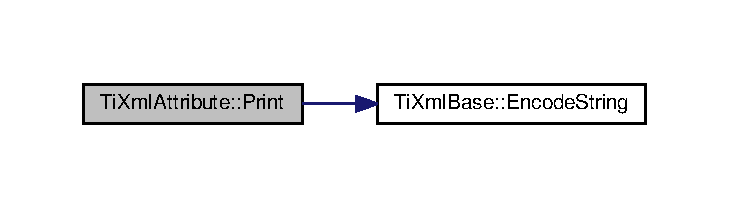
\includegraphics[width=350pt]{class_ti_xml_attribute_a19e6b6862a80b188571c47947e88d030_cgraph}
\end{center}
\end{figure}


\index{Ti\+Xml\+Attribute@{Ti\+Xml\+Attribute}!Query\+Double\+Value@{Query\+Double\+Value}}
\index{Query\+Double\+Value@{Query\+Double\+Value}!Ti\+Xml\+Attribute@{Ti\+Xml\+Attribute}}
\subsubsection[{\texorpdfstring{Query\+Double\+Value(double $\ast$\+\_\+value) const }{QueryDoubleValue(double *_value) const }}]{\setlength{\rightskip}{0pt plus 5cm}int Ti\+Xml\+Attribute\+::\+Query\+Double\+Value (
\begin{DoxyParamCaption}
\item[{double $\ast$}]{\+\_\+value}
\end{DoxyParamCaption}
) const}\hypertarget{class_ti_xml_attribute_ac87b2a8489906a5d7aa2875f20be3513}{}\label{class_ti_xml_attribute_ac87b2a8489906a5d7aa2875f20be3513}


Query\+Double\+Value examines the value string. See \hyperlink{class_ti_xml_attribute_ad6c93088ee21af41a107931223339344}{Query\+Int\+Value()}. 



Here is the caller graph for this function\+:
\nopagebreak
\begin{figure}[H]
\begin{center}
\leavevmode
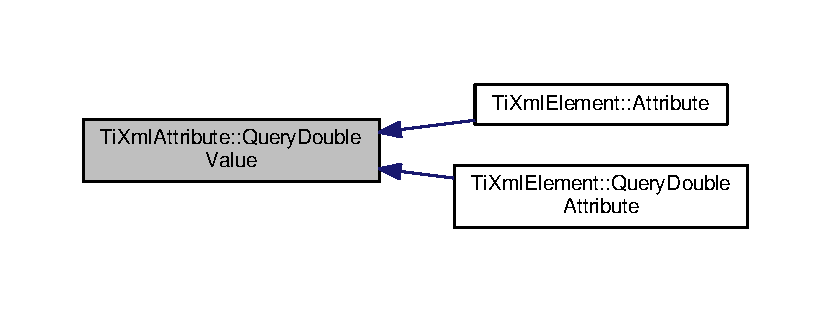
\includegraphics[width=350pt]{class_ti_xml_attribute_ac87b2a8489906a5d7aa2875f20be3513_icgraph}
\end{center}
\end{figure}


\index{Ti\+Xml\+Attribute@{Ti\+Xml\+Attribute}!Query\+Int\+Value@{Query\+Int\+Value}}
\index{Query\+Int\+Value@{Query\+Int\+Value}!Ti\+Xml\+Attribute@{Ti\+Xml\+Attribute}}
\subsubsection[{\texorpdfstring{Query\+Int\+Value(int $\ast$\+\_\+value) const }{QueryIntValue(int *_value) const }}]{\setlength{\rightskip}{0pt plus 5cm}int Ti\+Xml\+Attribute\+::\+Query\+Int\+Value (
\begin{DoxyParamCaption}
\item[{int $\ast$}]{\+\_\+value}
\end{DoxyParamCaption}
) const}\hypertarget{class_ti_xml_attribute_ad6c93088ee21af41a107931223339344}{}\label{class_ti_xml_attribute_ad6c93088ee21af41a107931223339344}
Query\+Int\+Value examines the value string. It is an alternative to the \hyperlink{class_ti_xml_attribute_aa1a20ad59dc7e89a0ab265396360d50f}{Int\+Value()} method with richer error checking. If the value is an integer, it is stored in \textquotesingle{}value\textquotesingle{} and the call returns T\+I\+X\+M\+L\+\_\+\+S\+U\+C\+C\+E\+SS. If it is not an integer, it returns T\+I\+X\+M\+L\+\_\+\+W\+R\+O\+N\+G\+\_\+\+T\+Y\+PE.

A specialized but useful call. Note that for success it returns 0, which is the opposite of almost all other Tiny\+Xml calls. 

Here is the caller graph for this function\+:
\nopagebreak
\begin{figure}[H]
\begin{center}
\leavevmode
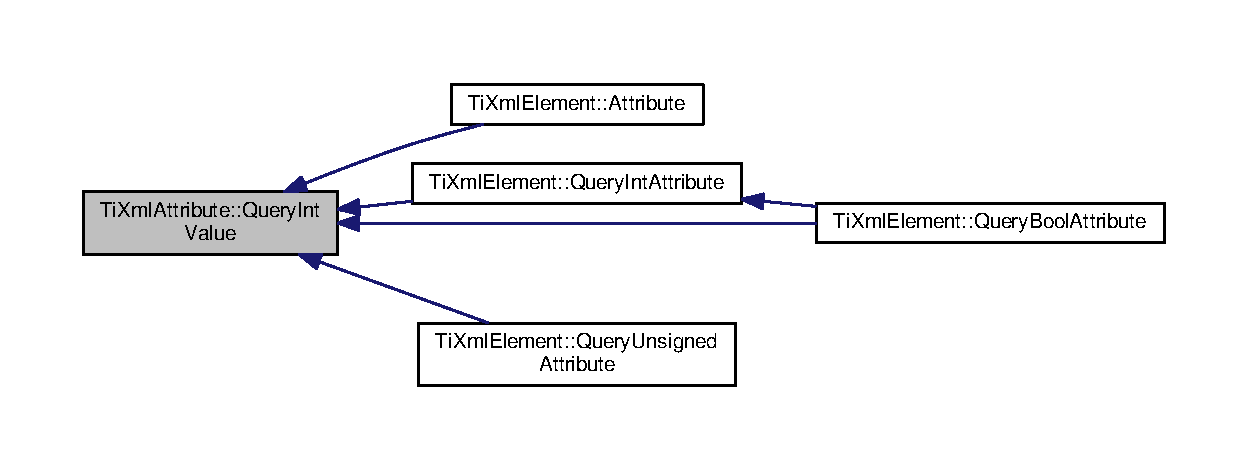
\includegraphics[width=350pt]{class_ti_xml_attribute_ad6c93088ee21af41a107931223339344_icgraph}
\end{center}
\end{figure}


\index{Ti\+Xml\+Attribute@{Ti\+Xml\+Attribute}!Set\+Document@{Set\+Document}}
\index{Set\+Document@{Set\+Document}!Ti\+Xml\+Attribute@{Ti\+Xml\+Attribute}}
\subsubsection[{\texorpdfstring{Set\+Document(\+Ti\+Xml\+Document $\ast$doc)}{SetDocument(TiXmlDocument *doc)}}]{\setlength{\rightskip}{0pt plus 5cm}void Ti\+Xml\+Attribute\+::\+Set\+Document (
\begin{DoxyParamCaption}
\item[{{\bf Ti\+Xml\+Document} $\ast$}]{doc}
\end{DoxyParamCaption}
)\hspace{0.3cm}{\ttfamily [inline]}}\hypertarget{class_ti_xml_attribute_ac12a94d4548302afb12f488ba101f7d1}{}\label{class_ti_xml_attribute_ac12a94d4548302afb12f488ba101f7d1}


Here is the caller graph for this function\+:
\nopagebreak
\begin{figure}[H]
\begin{center}
\leavevmode
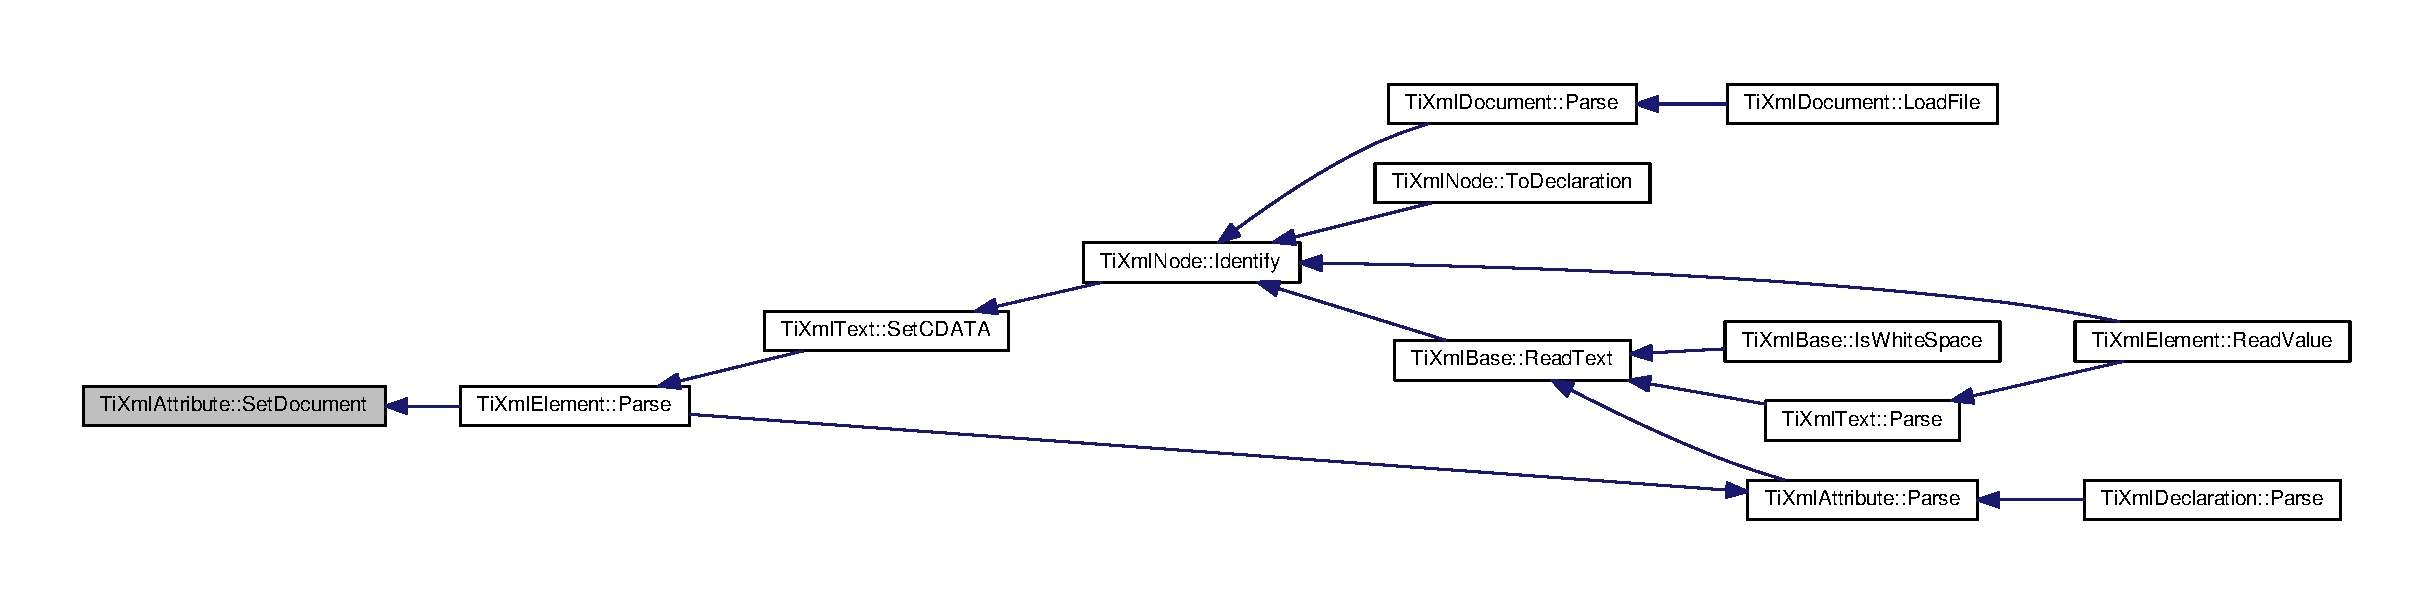
\includegraphics[width=350pt]{class_ti_xml_attribute_ac12a94d4548302afb12f488ba101f7d1_icgraph}
\end{center}
\end{figure}


\index{Ti\+Xml\+Attribute@{Ti\+Xml\+Attribute}!Set\+Double\+Value@{Set\+Double\+Value}}
\index{Set\+Double\+Value@{Set\+Double\+Value}!Ti\+Xml\+Attribute@{Ti\+Xml\+Attribute}}
\subsubsection[{\texorpdfstring{Set\+Double\+Value(double \+\_\+value)}{SetDoubleValue(double _value)}}]{\setlength{\rightskip}{0pt plus 5cm}void Ti\+Xml\+Attribute\+::\+Set\+Double\+Value (
\begin{DoxyParamCaption}
\item[{double}]{\+\_\+value}
\end{DoxyParamCaption}
)}\hypertarget{class_ti_xml_attribute_a0316da31373496c4368ad549bf711394}{}\label{class_ti_xml_attribute_a0316da31373496c4368ad549bf711394}


Set the value from a double. 



Here is the call graph for this function\+:
\nopagebreak
\begin{figure}[H]
\begin{center}
\leavevmode
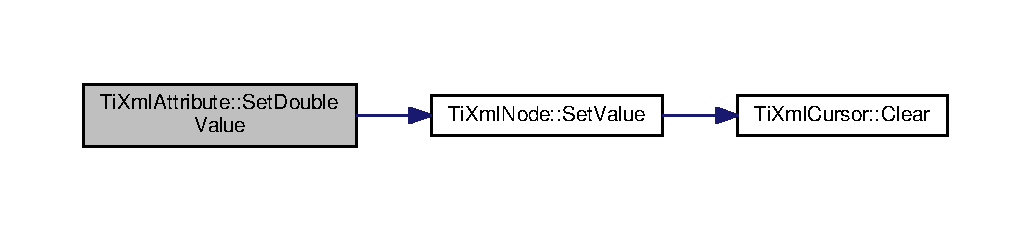
\includegraphics[width=350pt]{class_ti_xml_attribute_a0316da31373496c4368ad549bf711394_cgraph}
\end{center}
\end{figure}




Here is the caller graph for this function\+:
\nopagebreak
\begin{figure}[H]
\begin{center}
\leavevmode
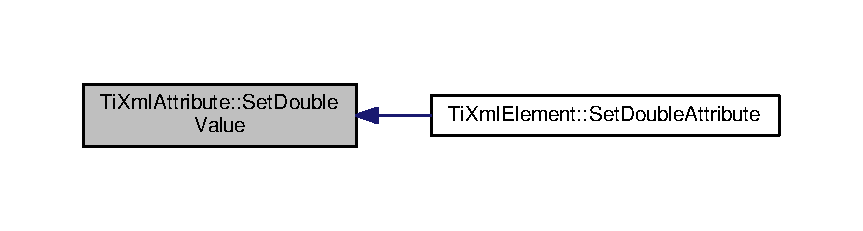
\includegraphics[width=350pt]{class_ti_xml_attribute_a0316da31373496c4368ad549bf711394_icgraph}
\end{center}
\end{figure}


\index{Ti\+Xml\+Attribute@{Ti\+Xml\+Attribute}!Set\+Int\+Value@{Set\+Int\+Value}}
\index{Set\+Int\+Value@{Set\+Int\+Value}!Ti\+Xml\+Attribute@{Ti\+Xml\+Attribute}}
\subsubsection[{\texorpdfstring{Set\+Int\+Value(int \+\_\+value)}{SetIntValue(int _value)}}]{\setlength{\rightskip}{0pt plus 5cm}void Ti\+Xml\+Attribute\+::\+Set\+Int\+Value (
\begin{DoxyParamCaption}
\item[{int}]{\+\_\+value}
\end{DoxyParamCaption}
)}\hypertarget{class_ti_xml_attribute_a7e065df640116a62ea4f4b7da5449cc8}{}\label{class_ti_xml_attribute_a7e065df640116a62ea4f4b7da5449cc8}


Set the value from an integer. 



Here is the call graph for this function\+:
\nopagebreak
\begin{figure}[H]
\begin{center}
\leavevmode
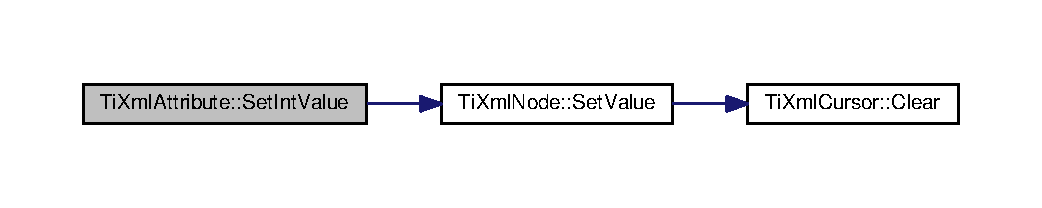
\includegraphics[width=350pt]{class_ti_xml_attribute_a7e065df640116a62ea4f4b7da5449cc8_cgraph}
\end{center}
\end{figure}




Here is the caller graph for this function\+:
\nopagebreak
\begin{figure}[H]
\begin{center}
\leavevmode
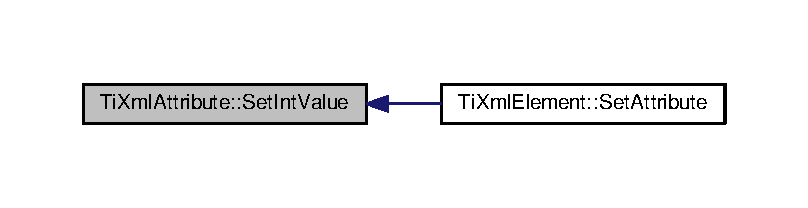
\includegraphics[width=350pt]{class_ti_xml_attribute_a7e065df640116a62ea4f4b7da5449cc8_icgraph}
\end{center}
\end{figure}


\index{Ti\+Xml\+Attribute@{Ti\+Xml\+Attribute}!Set\+Name@{Set\+Name}}
\index{Set\+Name@{Set\+Name}!Ti\+Xml\+Attribute@{Ti\+Xml\+Attribute}}
\subsubsection[{\texorpdfstring{Set\+Name(const char $\ast$\+\_\+name)}{SetName(const char *_name)}}]{\setlength{\rightskip}{0pt plus 5cm}void Ti\+Xml\+Attribute\+::\+Set\+Name (
\begin{DoxyParamCaption}
\item[{const char $\ast$}]{\+\_\+name}
\end{DoxyParamCaption}
)\hspace{0.3cm}{\ttfamily [inline]}}\hypertarget{class_ti_xml_attribute_ab7fa3d21ff8d7c5764cf9af15b667a99}{}\label{class_ti_xml_attribute_ab7fa3d21ff8d7c5764cf9af15b667a99}


Set the name of this attribute. 



Here is the caller graph for this function\+:
\nopagebreak
\begin{figure}[H]
\begin{center}
\leavevmode
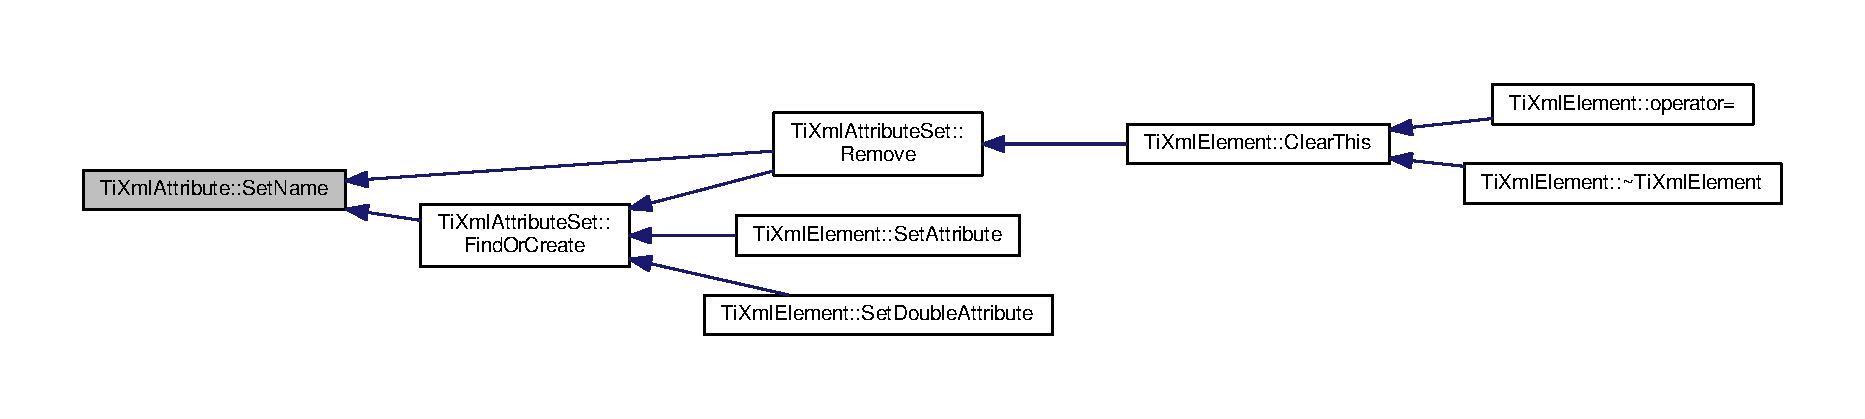
\includegraphics[width=350pt]{class_ti_xml_attribute_ab7fa3d21ff8d7c5764cf9af15b667a99_icgraph}
\end{center}
\end{figure}


\index{Ti\+Xml\+Attribute@{Ti\+Xml\+Attribute}!Set\+Value@{Set\+Value}}
\index{Set\+Value@{Set\+Value}!Ti\+Xml\+Attribute@{Ti\+Xml\+Attribute}}
\subsubsection[{\texorpdfstring{Set\+Value(const char $\ast$\+\_\+value)}{SetValue(const char *_value)}}]{\setlength{\rightskip}{0pt plus 5cm}void Ti\+Xml\+Attribute\+::\+Set\+Value (
\begin{DoxyParamCaption}
\item[{const char $\ast$}]{\+\_\+value}
\end{DoxyParamCaption}
)\hspace{0.3cm}{\ttfamily [inline]}}\hypertarget{class_ti_xml_attribute_a2dae44178f668b3cb48101be4f2236a0}{}\label{class_ti_xml_attribute_a2dae44178f668b3cb48101be4f2236a0}


Set the value. 



Here is the caller graph for this function\+:
\nopagebreak
\begin{figure}[H]
\begin{center}
\leavevmode
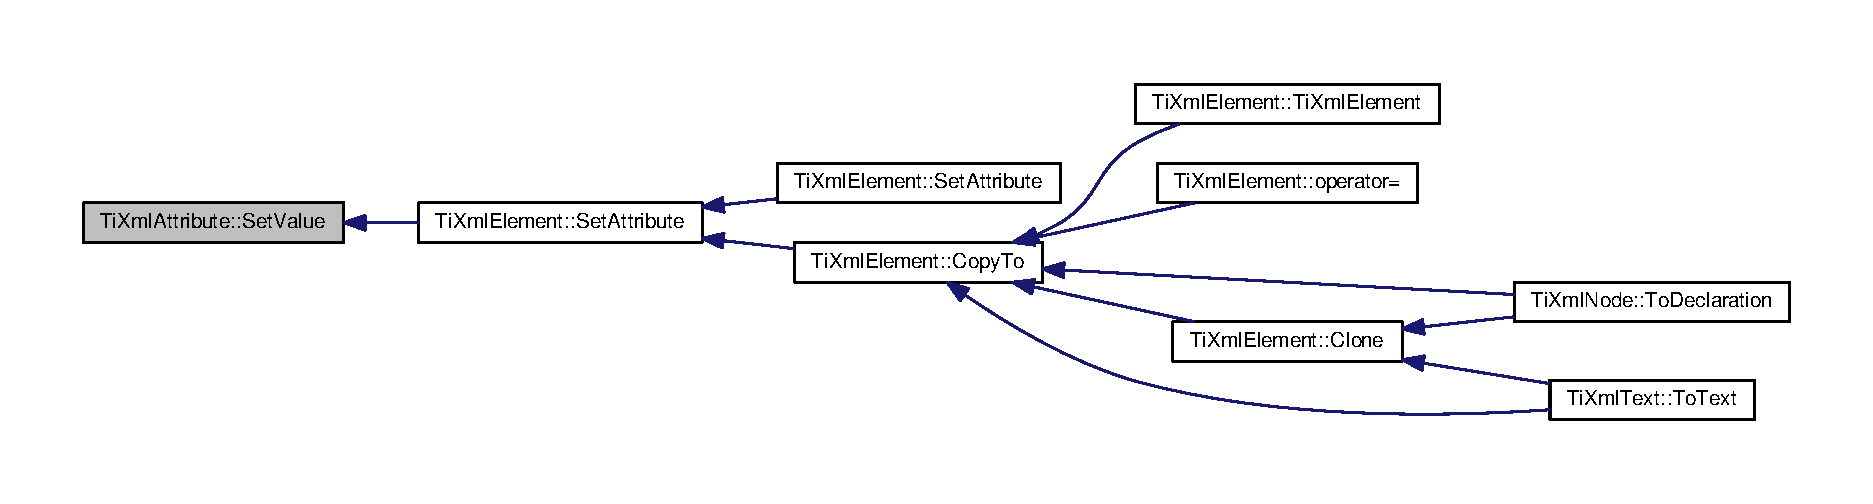
\includegraphics[width=350pt]{class_ti_xml_attribute_a2dae44178f668b3cb48101be4f2236a0_icgraph}
\end{center}
\end{figure}


\index{Ti\+Xml\+Attribute@{Ti\+Xml\+Attribute}!Value@{Value}}
\index{Value@{Value}!Ti\+Xml\+Attribute@{Ti\+Xml\+Attribute}}
\subsubsection[{\texorpdfstring{Value() const }{Value() const }}]{\setlength{\rightskip}{0pt plus 5cm}const char$\ast$ Ti\+Xml\+Attribute\+::\+Value (
\begin{DoxyParamCaption}
{}
\end{DoxyParamCaption}
) const\hspace{0.3cm}{\ttfamily [inline]}}\hypertarget{class_ti_xml_attribute_a0f874490eac8ca00ee0070765d0e97e3}{}\label{class_ti_xml_attribute_a0f874490eac8ca00ee0070765d0e97e3}


Return the value of this attribute. 



Here is the caller graph for this function\+:
\nopagebreak
\begin{figure}[H]
\begin{center}
\leavevmode
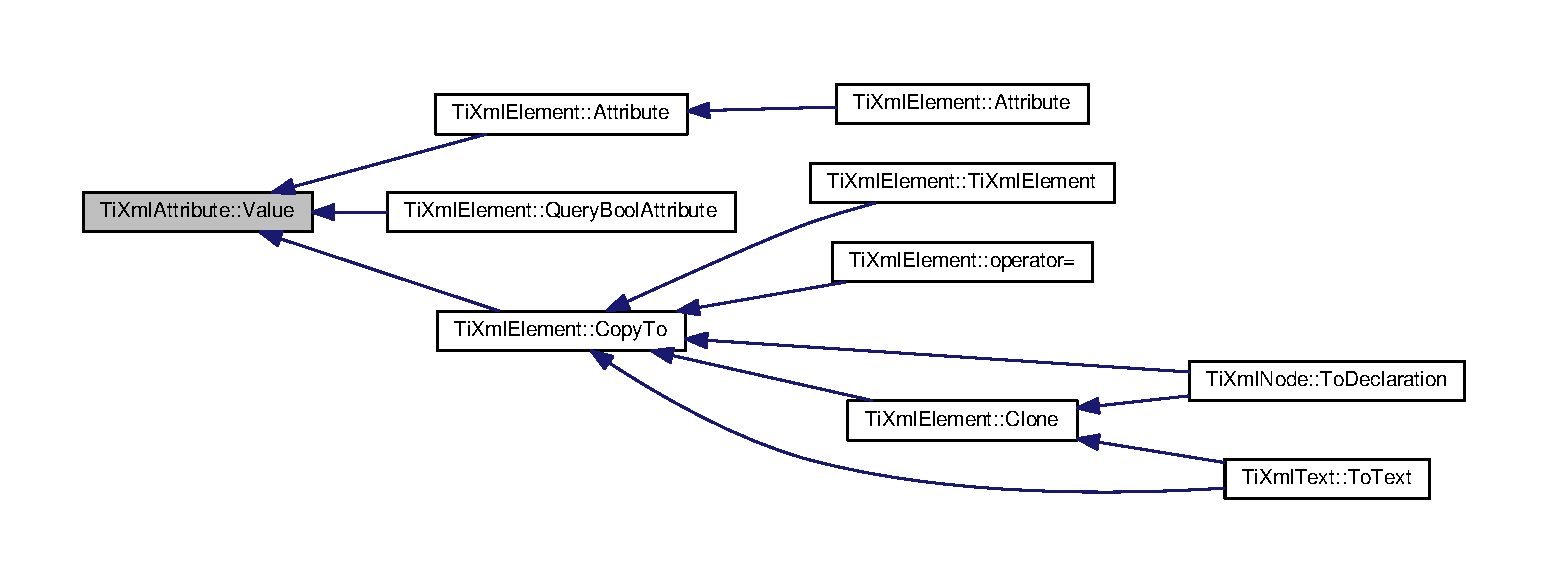
\includegraphics[width=350pt]{class_ti_xml_attribute_a0f874490eac8ca00ee0070765d0e97e3_icgraph}
\end{center}
\end{figure}




\subsection{Friends And Related Function Documentation}
\index{Ti\+Xml\+Attribute@{Ti\+Xml\+Attribute}!Ti\+Xml\+Attribute\+Set@{Ti\+Xml\+Attribute\+Set}}
\index{Ti\+Xml\+Attribute\+Set@{Ti\+Xml\+Attribute\+Set}!Ti\+Xml\+Attribute@{Ti\+Xml\+Attribute}}
\subsubsection[{\texorpdfstring{Ti\+Xml\+Attribute\+Set}{TiXmlAttributeSet}}]{\setlength{\rightskip}{0pt plus 5cm}friend class {\bf Ti\+Xml\+Attribute\+Set}\hspace{0.3cm}{\ttfamily [friend]}}\hypertarget{class_ti_xml_attribute_a35a7b7f89f708527677d5078d41ce0bf}{}\label{class_ti_xml_attribute_a35a7b7f89f708527677d5078d41ce0bf}


The documentation for this class was generated from the following files\+:\begin{DoxyCompactItemize}
\item 
/home/jonathan/\+Desktop/\+Project Software Engineering/\+Metronet/\+P\+S\+E/src/\hyperlink{tinyxml_8h}{tinyxml.\+h}\item 
/home/jonathan/\+Desktop/\+Project Software Engineering/\+Metronet/\+P\+S\+E/src/\hyperlink{tinyxml_8cpp}{tinyxml.\+cpp}\item 
/home/jonathan/\+Desktop/\+Project Software Engineering/\+Metronet/\+P\+S\+E/src/\hyperlink{tinyxmlparser_8cpp}{tinyxmlparser.\+cpp}\end{DoxyCompactItemize}

\hypertarget{class_ti_xml_attribute_set}{}\section{Ti\+Xml\+Attribute\+Set Class Reference}
\label{class_ti_xml_attribute_set}\index{Ti\+Xml\+Attribute\+Set@{Ti\+Xml\+Attribute\+Set}}


{\ttfamily \#include $<$tinyxml.\+h$>$}

\subsection*{Public Member Functions}
\begin{DoxyCompactItemize}
\item 
\hyperlink{class_ti_xml_attribute_set_a253c33b657cc85a07f7f060b02146c35}{Ti\+Xml\+Attribute\+Set} ()
\item 
\hyperlink{class_ti_xml_attribute_set_add463905dff96142a29fe16a01ecf28f}{$\sim$\+Ti\+Xml\+Attribute\+Set} ()
\item 
void \hyperlink{class_ti_xml_attribute_set_a745e50ddaae3bee93e4589321e0b9c1a}{Add} (\hyperlink{class_ti_xml_attribute}{Ti\+Xml\+Attribute} $\ast$attribute)
\item 
void \hyperlink{class_ti_xml_attribute_set_a924a73d071f2573f9060f0be57879c57}{Remove} (\hyperlink{class_ti_xml_attribute}{Ti\+Xml\+Attribute} $\ast$attribute)
\item 
const \hyperlink{class_ti_xml_attribute}{Ti\+Xml\+Attribute} $\ast$ \hyperlink{class_ti_xml_attribute_set_ae0636e88cedd4b09d61c451860f68598}{First} () const 
\item 
\hyperlink{class_ti_xml_attribute}{Ti\+Xml\+Attribute} $\ast$ \hyperlink{class_ti_xml_attribute_set_a99703bb08ca2aece2d7ef835de339ba0}{First} ()
\item 
const \hyperlink{class_ti_xml_attribute}{Ti\+Xml\+Attribute} $\ast$ \hyperlink{class_ti_xml_attribute_set_a7b3f3ccf39a97bc25539d3fcc540296a}{Last} () const 
\item 
\hyperlink{class_ti_xml_attribute}{Ti\+Xml\+Attribute} $\ast$ \hyperlink{class_ti_xml_attribute_set_ab4c4edfb2d74f6ea31aae096743bd6e0}{Last} ()
\item 
\hyperlink{class_ti_xml_attribute}{Ti\+Xml\+Attribute} $\ast$ \hyperlink{class_ti_xml_attribute_set_af3675cc2bfd0aea153cda1cfcdd1f77e}{Find} (const char $\ast$\+\_\+name) const 
\item 
\hyperlink{class_ti_xml_attribute}{Ti\+Xml\+Attribute} $\ast$ \hyperlink{class_ti_xml_attribute_set_a5e28f5d32f048fba85d04dc317495bdc}{Find\+Or\+Create} (const char $\ast$\+\_\+name)
\end{DoxyCompactItemize}


\subsection{Constructor \& Destructor Documentation}
\index{Ti\+Xml\+Attribute\+Set@{Ti\+Xml\+Attribute\+Set}!Ti\+Xml\+Attribute\+Set@{Ti\+Xml\+Attribute\+Set}}
\index{Ti\+Xml\+Attribute\+Set@{Ti\+Xml\+Attribute\+Set}!Ti\+Xml\+Attribute\+Set@{Ti\+Xml\+Attribute\+Set}}
\subsubsection[{\texorpdfstring{Ti\+Xml\+Attribute\+Set()}{TiXmlAttributeSet()}}]{\setlength{\rightskip}{0pt plus 5cm}Ti\+Xml\+Attribute\+Set\+::\+Ti\+Xml\+Attribute\+Set (
\begin{DoxyParamCaption}
{}
\end{DoxyParamCaption}
)}\hypertarget{class_ti_xml_attribute_set_a253c33b657cc85a07f7f060b02146c35}{}\label{class_ti_xml_attribute_set_a253c33b657cc85a07f7f060b02146c35}
\index{Ti\+Xml\+Attribute\+Set@{Ti\+Xml\+Attribute\+Set}!````~Ti\+Xml\+Attribute\+Set@{$\sim$\+Ti\+Xml\+Attribute\+Set}}
\index{````~Ti\+Xml\+Attribute\+Set@{$\sim$\+Ti\+Xml\+Attribute\+Set}!Ti\+Xml\+Attribute\+Set@{Ti\+Xml\+Attribute\+Set}}
\subsubsection[{\texorpdfstring{$\sim$\+Ti\+Xml\+Attribute\+Set()}{~TiXmlAttributeSet()}}]{\setlength{\rightskip}{0pt plus 5cm}Ti\+Xml\+Attribute\+Set\+::$\sim$\+Ti\+Xml\+Attribute\+Set (
\begin{DoxyParamCaption}
{}
\end{DoxyParamCaption}
)}\hypertarget{class_ti_xml_attribute_set_add463905dff96142a29fe16a01ecf28f}{}\label{class_ti_xml_attribute_set_add463905dff96142a29fe16a01ecf28f}


\subsection{Member Function Documentation}
\index{Ti\+Xml\+Attribute\+Set@{Ti\+Xml\+Attribute\+Set}!Add@{Add}}
\index{Add@{Add}!Ti\+Xml\+Attribute\+Set@{Ti\+Xml\+Attribute\+Set}}
\subsubsection[{\texorpdfstring{Add(\+Ti\+Xml\+Attribute $\ast$attribute)}{Add(TiXmlAttribute *attribute)}}]{\setlength{\rightskip}{0pt plus 5cm}void Ti\+Xml\+Attribute\+Set\+::\+Add (
\begin{DoxyParamCaption}
\item[{{\bf Ti\+Xml\+Attribute} $\ast$}]{attribute}
\end{DoxyParamCaption}
)}\hypertarget{class_ti_xml_attribute_set_a745e50ddaae3bee93e4589321e0b9c1a}{}\label{class_ti_xml_attribute_set_a745e50ddaae3bee93e4589321e0b9c1a}


Here is the call graph for this function\+:
\nopagebreak
\begin{figure}[H]
\begin{center}
\leavevmode
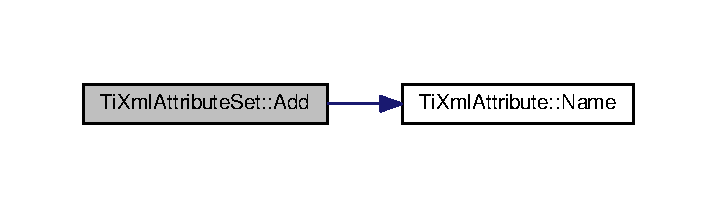
\includegraphics[width=344pt]{class_ti_xml_attribute_set_a745e50ddaae3bee93e4589321e0b9c1a_cgraph}
\end{center}
\end{figure}


\index{Ti\+Xml\+Attribute\+Set@{Ti\+Xml\+Attribute\+Set}!Find@{Find}}
\index{Find@{Find}!Ti\+Xml\+Attribute\+Set@{Ti\+Xml\+Attribute\+Set}}
\subsubsection[{\texorpdfstring{Find(const char $\ast$\+\_\+name) const }{Find(const char *_name) const }}]{\setlength{\rightskip}{0pt plus 5cm}{\bf Ti\+Xml\+Attribute} $\ast$ Ti\+Xml\+Attribute\+Set\+::\+Find (
\begin{DoxyParamCaption}
\item[{const char $\ast$}]{\+\_\+name}
\end{DoxyParamCaption}
) const}\hypertarget{class_ti_xml_attribute_set_af3675cc2bfd0aea153cda1cfcdd1f77e}{}\label{class_ti_xml_attribute_set_af3675cc2bfd0aea153cda1cfcdd1f77e}


Here is the caller graph for this function\+:
\nopagebreak
\begin{figure}[H]
\begin{center}
\leavevmode
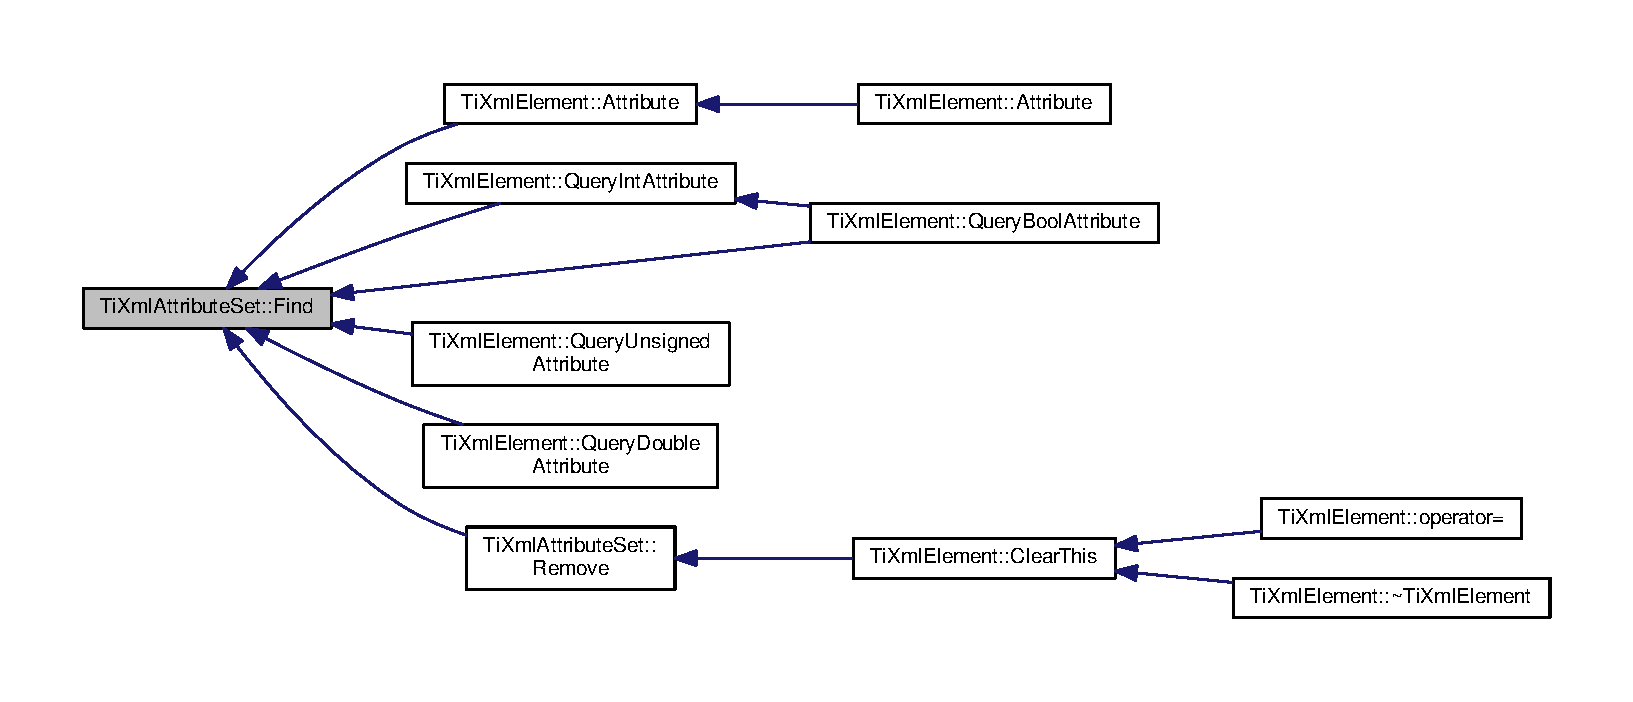
\includegraphics[width=350pt]{class_ti_xml_attribute_set_af3675cc2bfd0aea153cda1cfcdd1f77e_icgraph}
\end{center}
\end{figure}


\index{Ti\+Xml\+Attribute\+Set@{Ti\+Xml\+Attribute\+Set}!Find\+Or\+Create@{Find\+Or\+Create}}
\index{Find\+Or\+Create@{Find\+Or\+Create}!Ti\+Xml\+Attribute\+Set@{Ti\+Xml\+Attribute\+Set}}
\subsubsection[{\texorpdfstring{Find\+Or\+Create(const char $\ast$\+\_\+name)}{FindOrCreate(const char *_name)}}]{\setlength{\rightskip}{0pt plus 5cm}{\bf Ti\+Xml\+Attribute} $\ast$ Ti\+Xml\+Attribute\+Set\+::\+Find\+Or\+Create (
\begin{DoxyParamCaption}
\item[{const char $\ast$}]{\+\_\+name}
\end{DoxyParamCaption}
)}\hypertarget{class_ti_xml_attribute_set_a5e28f5d32f048fba85d04dc317495bdc}{}\label{class_ti_xml_attribute_set_a5e28f5d32f048fba85d04dc317495bdc}


Here is the call graph for this function\+:
\nopagebreak
\begin{figure}[H]
\begin{center}
\leavevmode
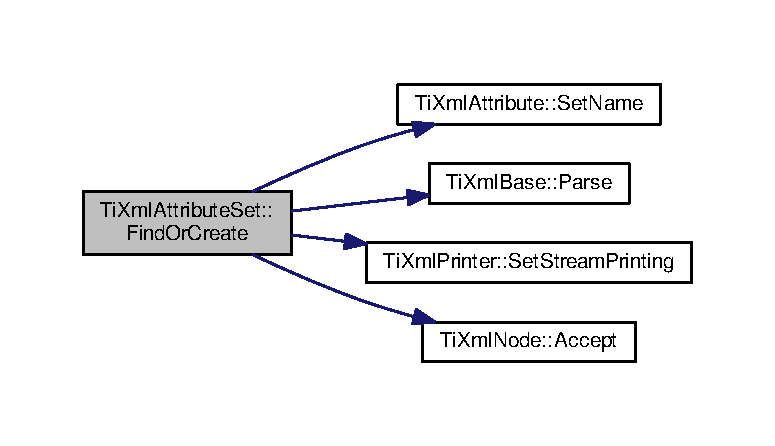
\includegraphics[width=350pt]{class_ti_xml_attribute_set_a5e28f5d32f048fba85d04dc317495bdc_cgraph}
\end{center}
\end{figure}




Here is the caller graph for this function\+:
\nopagebreak
\begin{figure}[H]
\begin{center}
\leavevmode
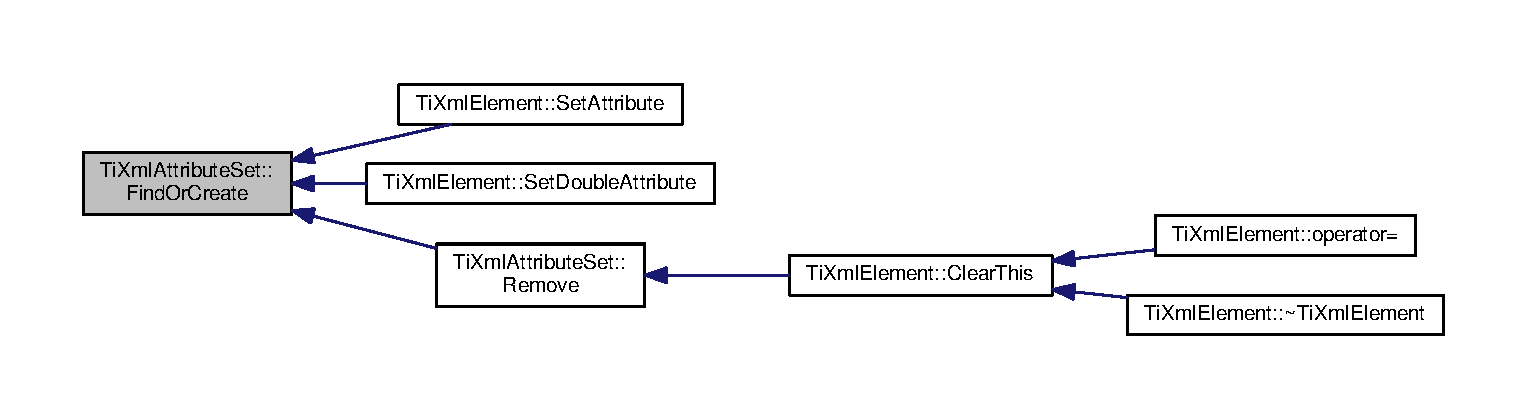
\includegraphics[width=350pt]{class_ti_xml_attribute_set_a5e28f5d32f048fba85d04dc317495bdc_icgraph}
\end{center}
\end{figure}


\index{Ti\+Xml\+Attribute\+Set@{Ti\+Xml\+Attribute\+Set}!First@{First}}
\index{First@{First}!Ti\+Xml\+Attribute\+Set@{Ti\+Xml\+Attribute\+Set}}
\subsubsection[{\texorpdfstring{First() const }{First() const }}]{\setlength{\rightskip}{0pt plus 5cm}const {\bf Ti\+Xml\+Attribute}$\ast$ Ti\+Xml\+Attribute\+Set\+::\+First (
\begin{DoxyParamCaption}
{}
\end{DoxyParamCaption}
) const\hspace{0.3cm}{\ttfamily [inline]}}\hypertarget{class_ti_xml_attribute_set_ae0636e88cedd4b09d61c451860f68598}{}\label{class_ti_xml_attribute_set_ae0636e88cedd4b09d61c451860f68598}


Here is the caller graph for this function\+:
\nopagebreak
\begin{figure}[H]
\begin{center}
\leavevmode
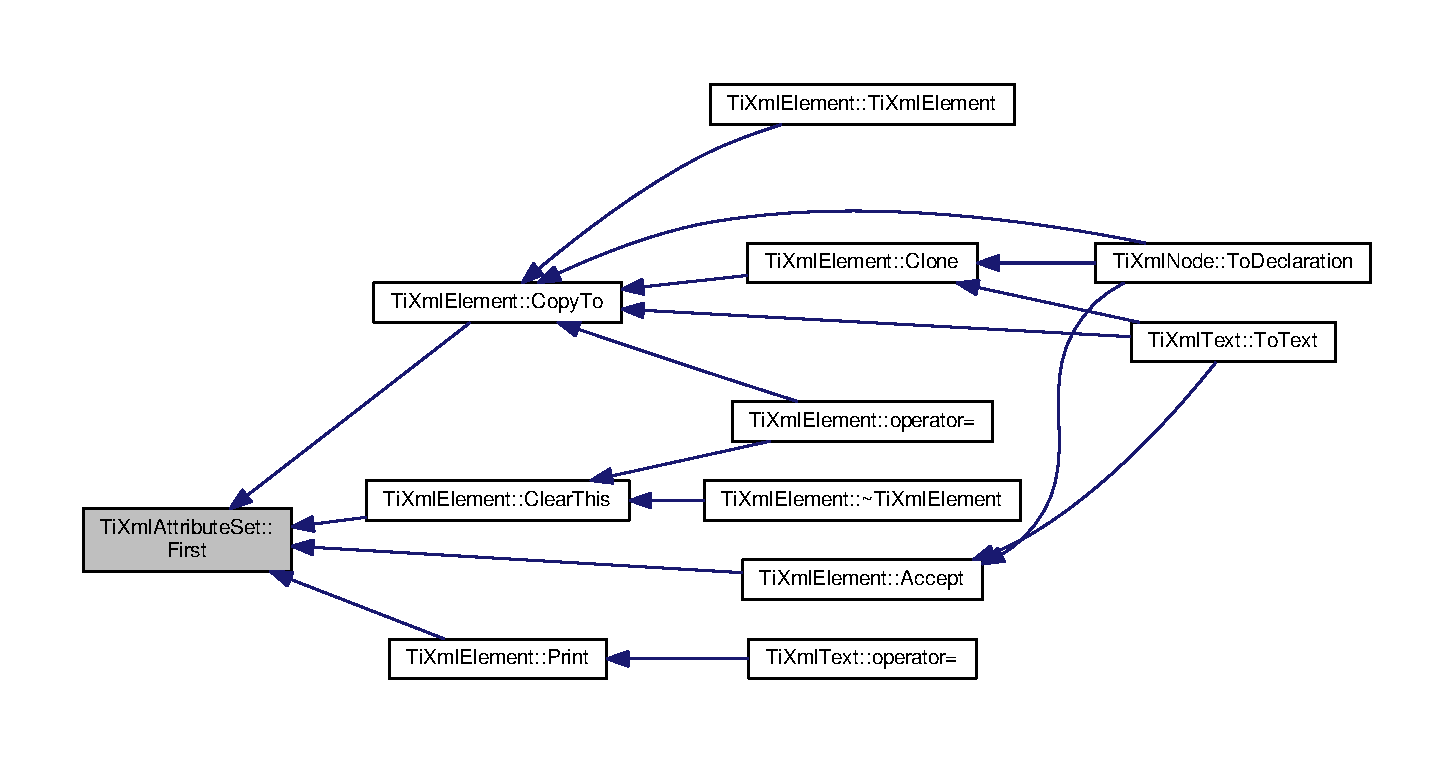
\includegraphics[width=350pt]{class_ti_xml_attribute_set_ae0636e88cedd4b09d61c451860f68598_icgraph}
\end{center}
\end{figure}


\index{Ti\+Xml\+Attribute\+Set@{Ti\+Xml\+Attribute\+Set}!First@{First}}
\index{First@{First}!Ti\+Xml\+Attribute\+Set@{Ti\+Xml\+Attribute\+Set}}
\subsubsection[{\texorpdfstring{First()}{First()}}]{\setlength{\rightskip}{0pt plus 5cm}{\bf Ti\+Xml\+Attribute}$\ast$ Ti\+Xml\+Attribute\+Set\+::\+First (
\begin{DoxyParamCaption}
{}
\end{DoxyParamCaption}
)\hspace{0.3cm}{\ttfamily [inline]}}\hypertarget{class_ti_xml_attribute_set_a99703bb08ca2aece2d7ef835de339ba0}{}\label{class_ti_xml_attribute_set_a99703bb08ca2aece2d7ef835de339ba0}
\index{Ti\+Xml\+Attribute\+Set@{Ti\+Xml\+Attribute\+Set}!Last@{Last}}
\index{Last@{Last}!Ti\+Xml\+Attribute\+Set@{Ti\+Xml\+Attribute\+Set}}
\subsubsection[{\texorpdfstring{Last() const }{Last() const }}]{\setlength{\rightskip}{0pt plus 5cm}const {\bf Ti\+Xml\+Attribute}$\ast$ Ti\+Xml\+Attribute\+Set\+::\+Last (
\begin{DoxyParamCaption}
{}
\end{DoxyParamCaption}
) const\hspace{0.3cm}{\ttfamily [inline]}}\hypertarget{class_ti_xml_attribute_set_a7b3f3ccf39a97bc25539d3fcc540296a}{}\label{class_ti_xml_attribute_set_a7b3f3ccf39a97bc25539d3fcc540296a}
\index{Ti\+Xml\+Attribute\+Set@{Ti\+Xml\+Attribute\+Set}!Last@{Last}}
\index{Last@{Last}!Ti\+Xml\+Attribute\+Set@{Ti\+Xml\+Attribute\+Set}}
\subsubsection[{\texorpdfstring{Last()}{Last()}}]{\setlength{\rightskip}{0pt plus 5cm}{\bf Ti\+Xml\+Attribute}$\ast$ Ti\+Xml\+Attribute\+Set\+::\+Last (
\begin{DoxyParamCaption}
{}
\end{DoxyParamCaption}
)\hspace{0.3cm}{\ttfamily [inline]}}\hypertarget{class_ti_xml_attribute_set_ab4c4edfb2d74f6ea31aae096743bd6e0}{}\label{class_ti_xml_attribute_set_ab4c4edfb2d74f6ea31aae096743bd6e0}
\index{Ti\+Xml\+Attribute\+Set@{Ti\+Xml\+Attribute\+Set}!Remove@{Remove}}
\index{Remove@{Remove}!Ti\+Xml\+Attribute\+Set@{Ti\+Xml\+Attribute\+Set}}
\subsubsection[{\texorpdfstring{Remove(\+Ti\+Xml\+Attribute $\ast$attribute)}{Remove(TiXmlAttribute *attribute)}}]{\setlength{\rightskip}{0pt plus 5cm}void Ti\+Xml\+Attribute\+Set\+::\+Remove (
\begin{DoxyParamCaption}
\item[{{\bf Ti\+Xml\+Attribute} $\ast$}]{attribute}
\end{DoxyParamCaption}
)}\hypertarget{class_ti_xml_attribute_set_a924a73d071f2573f9060f0be57879c57}{}\label{class_ti_xml_attribute_set_a924a73d071f2573f9060f0be57879c57}


Here is the call graph for this function\+:
\nopagebreak
\begin{figure}[H]
\begin{center}
\leavevmode
\includegraphics[width=350pt]{class_ti_xml_attribute_set_a924a73d071f2573f9060f0be57879c57_cgraph}
\end{center}
\end{figure}




Here is the caller graph for this function\+:
\nopagebreak
\begin{figure}[H]
\begin{center}
\leavevmode
\includegraphics[width=350pt]{class_ti_xml_attribute_set_a924a73d071f2573f9060f0be57879c57_icgraph}
\end{center}
\end{figure}




The documentation for this class was generated from the following files\+:\begin{DoxyCompactItemize}
\item 
/home/jonathan/\+Desktop/\+Project Software Engineering/\+Metronet/\+P\+S\+E/src/\hyperlink{tinyxml_8h}{tinyxml.\+h}\item 
/home/jonathan/\+Desktop/\+Project Software Engineering/\+Metronet/\+P\+S\+E/src/\hyperlink{tinyxml_8cpp}{tinyxml.\+cpp}\end{DoxyCompactItemize}

\hypertarget{class_ti_xml_base}{}\section{Ti\+Xml\+Base Class Reference}
\label{class_ti_xml_base}\index{Ti\+Xml\+Base@{Ti\+Xml\+Base}}


{\ttfamily \#include $<$tinyxml.\+h$>$}



Inheritance diagram for Ti\+Xml\+Base\+:\nopagebreak
\begin{figure}[H]
\begin{center}
\leavevmode
\includegraphics[width=350pt]{class_ti_xml_base__inherit__graph}
\end{center}
\end{figure}


Collaboration diagram for Ti\+Xml\+Base\+:\nopagebreak
\begin{figure}[H]
\begin{center}
\leavevmode
\includegraphics[width=153pt]{class_ti_xml_base__coll__graph}
\end{center}
\end{figure}
\subsection*{Public Types}
\begin{DoxyCompactItemize}
\item 
enum \{ \\*
\hyperlink{class_ti_xml_base_a9a7e9344415956ab96e8c75f6a0bbd48a750a76ca602241c416d5ec357d55fba1}{T\+I\+X\+M\+L\+\_\+\+N\+O\+\_\+\+E\+R\+R\+OR} = 0, 
\hyperlink{class_ti_xml_base_a9a7e9344415956ab96e8c75f6a0bbd48abcabc1b8efabeda1cc4352aa73d64390}{T\+I\+X\+M\+L\+\_\+\+E\+R\+R\+OR}, 
\hyperlink{class_ti_xml_base_a9a7e9344415956ab96e8c75f6a0bbd48ab803949b8f12e03b5b57f86d9c52b614}{T\+I\+X\+M\+L\+\_\+\+E\+R\+R\+O\+R\+\_\+\+O\+P\+E\+N\+I\+N\+G\+\_\+\+F\+I\+LE}, 
\hyperlink{class_ti_xml_base_a9a7e9344415956ab96e8c75f6a0bbd48a5cbfcf7fe5e67f0cd1aef98deac55dd2}{T\+I\+X\+M\+L\+\_\+\+E\+R\+R\+O\+R\+\_\+\+P\+A\+R\+S\+I\+N\+G\+\_\+\+E\+L\+E\+M\+E\+NT}, 
\\*
\hyperlink{class_ti_xml_base_a9a7e9344415956ab96e8c75f6a0bbd48adcc31ca78a9d507a88c9fafb3d18a3c4}{T\+I\+X\+M\+L\+\_\+\+E\+R\+R\+O\+R\+\_\+\+F\+A\+I\+L\+E\+D\+\_\+\+T\+O\+\_\+\+R\+E\+A\+D\+\_\+\+E\+L\+E\+M\+E\+N\+T\+\_\+\+N\+A\+ME}, 
\hyperlink{class_ti_xml_base_a9a7e9344415956ab96e8c75f6a0bbd48afefdc75db23215e846605a2b5af0c2d3}{T\+I\+X\+M\+L\+\_\+\+E\+R\+R\+O\+R\+\_\+\+R\+E\+A\+D\+I\+N\+G\+\_\+\+E\+L\+E\+M\+E\+N\+T\+\_\+\+V\+A\+L\+UE}, 
\hyperlink{class_ti_xml_base_a9a7e9344415956ab96e8c75f6a0bbd48a670fac23171b64829f90639cc3696d6e}{T\+I\+X\+M\+L\+\_\+\+E\+R\+R\+O\+R\+\_\+\+R\+E\+A\+D\+I\+N\+G\+\_\+\+A\+T\+T\+R\+I\+B\+U\+T\+ES}, 
\hyperlink{class_ti_xml_base_a9a7e9344415956ab96e8c75f6a0bbd48a5f2aee664733a20f13f6f77556b9fa85}{T\+I\+X\+M\+L\+\_\+\+E\+R\+R\+O\+R\+\_\+\+P\+A\+R\+S\+I\+N\+G\+\_\+\+E\+M\+P\+TY}, 
\\*
\hyperlink{class_ti_xml_base_a9a7e9344415956ab96e8c75f6a0bbd48a175f7c72e2f9630bb96ef5137b325502}{T\+I\+X\+M\+L\+\_\+\+E\+R\+R\+O\+R\+\_\+\+R\+E\+A\+D\+I\+N\+G\+\_\+\+E\+N\+D\+\_\+\+T\+AG}, 
\hyperlink{class_ti_xml_base_a9a7e9344415956ab96e8c75f6a0bbd48a24c814fdcf1d84704869e6f76b19cb6e}{T\+I\+X\+M\+L\+\_\+\+E\+R\+R\+O\+R\+\_\+\+P\+A\+R\+S\+I\+N\+G\+\_\+\+U\+N\+K\+N\+O\+WN}, 
\hyperlink{class_ti_xml_base_a9a7e9344415956ab96e8c75f6a0bbd48a72e3072a44be499edb89593f6ce10f6c}{T\+I\+X\+M\+L\+\_\+\+E\+R\+R\+O\+R\+\_\+\+P\+A\+R\+S\+I\+N\+G\+\_\+\+C\+O\+M\+M\+E\+NT}, 
\hyperlink{class_ti_xml_base_a9a7e9344415956ab96e8c75f6a0bbd48a4c200f9d125027ab449e2be7be471ba0}{T\+I\+X\+M\+L\+\_\+\+E\+R\+R\+O\+R\+\_\+\+P\+A\+R\+S\+I\+N\+G\+\_\+\+D\+E\+C\+L\+A\+R\+A\+T\+I\+ON}, 
\\*
\hyperlink{class_ti_xml_base_a9a7e9344415956ab96e8c75f6a0bbd48ab345f3e42e6ae9cdedee2b95e4d461b9}{T\+I\+X\+M\+L\+\_\+\+E\+R\+R\+O\+R\+\_\+\+D\+O\+C\+U\+M\+E\+N\+T\+\_\+\+E\+M\+P\+TY}, 
\hyperlink{class_ti_xml_base_a9a7e9344415956ab96e8c75f6a0bbd48ade7edbad3a94a6c161cac2638f380e17}{T\+I\+X\+M\+L\+\_\+\+E\+R\+R\+O\+R\+\_\+\+E\+M\+B\+E\+D\+D\+E\+D\+\_\+\+N\+U\+LL}, 
\hyperlink{class_ti_xml_base_a9a7e9344415956ab96e8c75f6a0bbd48aab2c858631b5d38eae1e6675949b9cd4}{T\+I\+X\+M\+L\+\_\+\+E\+R\+R\+O\+R\+\_\+\+P\+A\+R\+S\+I\+N\+G\+\_\+\+C\+D\+A\+TA}, 
\hyperlink{class_ti_xml_base_a9a7e9344415956ab96e8c75f6a0bbd48a679b15d950f29257700a724bb118c34d}{T\+I\+X\+M\+L\+\_\+\+E\+R\+R\+O\+R\+\_\+\+D\+O\+C\+U\+M\+E\+N\+T\+\_\+\+T\+O\+P\+\_\+\+O\+N\+LY}, 
\\*
\hyperlink{class_ti_xml_base_a9a7e9344415956ab96e8c75f6a0bbd48a14552894942250efcec6b00dc52fc48a}{T\+I\+X\+M\+L\+\_\+\+E\+R\+R\+O\+R\+\_\+\+S\+T\+R\+I\+N\+G\+\_\+\+C\+O\+U\+NT}
 \}
\end{DoxyCompactItemize}
\subsection*{Public Member Functions}
\begin{DoxyCompactItemize}
\item 
\hyperlink{class_ti_xml_base_ac6753fe8a2c89669038fcf281cb301bf}{Ti\+Xml\+Base} ()
\item 
virtual \hyperlink{class_ti_xml_base_ad1837ecb25a913612fa1115f090cbb56}{$\sim$\+Ti\+Xml\+Base} ()
\item 
virtual void \hyperlink{class_ti_xml_base_a0de56b3f2ef14c65091a3b916437b512}{Print} (F\+I\+LE $\ast$cfile, int depth) const =0
\item 
int \hyperlink{class_ti_xml_base_a024bceb070188df92c2a8d8852dd0853}{Row} () const 
\item 
int \hyperlink{class_ti_xml_base_ab54bfb9b70fe6dd276e7b279cab7f003}{Column} () const 
\begin{DoxyCompactList}\small\item\em See \hyperlink{class_ti_xml_base_a024bceb070188df92c2a8d8852dd0853}{Row()} \end{DoxyCompactList}\item 
void \hyperlink{class_ti_xml_base_ac6b3e0f790930d4970ec30764e937b5d}{Set\+User\+Data} (void $\ast$user)
\begin{DoxyCompactList}\small\item\em Set a pointer to arbitrary user data. \end{DoxyCompactList}\item 
void $\ast$ \hyperlink{class_ti_xml_base_a6559a530ca6763fc301a14d77ed28c17}{Get\+User\+Data} ()
\begin{DoxyCompactList}\small\item\em Get a pointer to arbitrary user data. \end{DoxyCompactList}\item 
const void $\ast$ \hyperlink{class_ti_xml_base_ad0120210e4680ef2088601753ce0ede4}{Get\+User\+Data} () const 
\begin{DoxyCompactList}\small\item\em Get a pointer to arbitrary user data. \end{DoxyCompactList}\item 
virtual const char $\ast$ \hyperlink{class_ti_xml_base_a00e4edb0219d00a1379c856e5a1d2025}{Parse} (const char $\ast$p, Ti\+Xml\+Parsing\+Data $\ast$data, \hyperlink{tinyxml_8h_a88d51847a13ee0f4b4d320d03d2c4d96}{Ti\+Xml\+Encoding} encoding)=0
\end{DoxyCompactItemize}
\subsection*{Static Public Member Functions}
\begin{DoxyCompactItemize}
\item 
static void \hyperlink{class_ti_xml_base_a0f799ec645bfb8d8a969e83478f379c1}{Set\+Condense\+White\+Space} (bool condense)
\item 
static bool \hyperlink{class_ti_xml_base_ad4b1472531c647a25b1840a87ae42438}{Is\+White\+Space\+Condensed} ()
\begin{DoxyCompactList}\small\item\em Return the current white space setting. \end{DoxyCompactList}\item 
static void \hyperlink{class_ti_xml_base_a32ed202562b58de64c7d799ca3c9db98}{Encode\+String} (const \hyperlink{tinyxml_8h_a92bada05fd84d9a0c9a5bbe53de26887}{T\+I\+X\+M\+L\+\_\+\+S\+T\+R\+I\+NG} \&str, \hyperlink{tinyxml_8h_a92bada05fd84d9a0c9a5bbe53de26887}{T\+I\+X\+M\+L\+\_\+\+S\+T\+R\+I\+NG} $\ast$out)
\end{DoxyCompactItemize}
\subsection*{Static Public Attributes}
\begin{DoxyCompactItemize}
\item 
static const int \hyperlink{class_ti_xml_base_a727583b4ed4342a3ad78cdc39b819af4}{utf8\+Byte\+Table} \mbox{[}256\mbox{]}
\end{DoxyCompactItemize}
\subsection*{Static Protected Member Functions}
\begin{DoxyCompactItemize}
\item 
static const char $\ast$ \hyperlink{class_ti_xml_base_a6849556ca97c0a172c6b996f08287ee1}{Skip\+White\+Space} (const char $\ast$, \hyperlink{tinyxml_8h_a88d51847a13ee0f4b4d320d03d2c4d96}{Ti\+Xml\+Encoding} encoding)
\item 
static bool \hyperlink{class_ti_xml_base_af56296d561c0bab4bc8e198cdcf5c48e}{Is\+White\+Space} (char c)
\item 
static bool \hyperlink{class_ti_xml_base_a3de391ea9f4c4a8aa10d04480b048795}{Is\+White\+Space} (int c)
\item 
static const char $\ast$ \hyperlink{class_ti_xml_base_a910e1664e0d6a4da5d4d1bfaa51130fe}{Read\+Name} (const char $\ast$p, \hyperlink{tinyxml_8h_a92bada05fd84d9a0c9a5bbe53de26887}{T\+I\+X\+M\+L\+\_\+\+S\+T\+R\+I\+NG} $\ast$name, \hyperlink{tinyxml_8h_a88d51847a13ee0f4b4d320d03d2c4d96}{Ti\+Xml\+Encoding} encoding)
\item 
static const char $\ast$ \hyperlink{class_ti_xml_base_a7f9beef90db30fa63dd35b3f992a30ca}{Read\+Text} (const char $\ast$in, \hyperlink{tinyxml_8h_a92bada05fd84d9a0c9a5bbe53de26887}{T\+I\+X\+M\+L\+\_\+\+S\+T\+R\+I\+NG} $\ast$text, bool ignore\+White\+Space, const char $\ast$end\+Tag, bool ignore\+Case, \hyperlink{tinyxml_8h_a88d51847a13ee0f4b4d320d03d2c4d96}{Ti\+Xml\+Encoding} encoding)
\item 
static const char $\ast$ \hyperlink{class_ti_xml_base_a44f75cc7a45a97a09e509dc4c8c127e0}{Get\+Entity} (const char $\ast$in, char $\ast$value, int $\ast$length, \hyperlink{tinyxml_8h_a88d51847a13ee0f4b4d320d03d2c4d96}{Ti\+Xml\+Encoding} encoding)
\item 
static const char $\ast$ \hyperlink{class_ti_xml_base_a5b0fde72d6f662ae1fd6303195d2159b}{Get\+Char} (const char $\ast$p, char $\ast$\+\_\+value, int $\ast$length, \hyperlink{tinyxml_8h_a88d51847a13ee0f4b4d320d03d2c4d96}{Ti\+Xml\+Encoding} encoding)
\item 
static bool \hyperlink{class_ti_xml_base_ad668006b550c011d05072dd4fc16577d}{String\+Equal} (const char $\ast$p, const char $\ast$end\+Tag, bool ignore\+Case, \hyperlink{tinyxml_8h_a88d51847a13ee0f4b4d320d03d2c4d96}{Ti\+Xml\+Encoding} encoding)
\item 
static int \hyperlink{class_ti_xml_base_ac95c7391b56770ff134644b1d74a1a4e}{Is\+Alpha} (unsigned char any\+Byte, \hyperlink{tinyxml_8h_a88d51847a13ee0f4b4d320d03d2c4d96}{Ti\+Xml\+Encoding} encoding)
\item 
static int \hyperlink{class_ti_xml_base_ae85b1b5e0351c80f2d795ca7005e79b7}{Is\+Alpha\+Num} (unsigned char any\+Byte, \hyperlink{tinyxml_8h_a88d51847a13ee0f4b4d320d03d2c4d96}{Ti\+Xml\+Encoding} encoding)
\item 
static int \hyperlink{class_ti_xml_base_a799f17405a86a5c2029618e85f11a097}{To\+Lower} (int v, \hyperlink{tinyxml_8h_a88d51847a13ee0f4b4d320d03d2c4d96}{Ti\+Xml\+Encoding} encoding)
\item 
static void \hyperlink{class_ti_xml_base_ad2b292fa401b8a5b8e6536de9261a3bb}{Convert\+U\+T\+F32\+To\+U\+T\+F8} (unsigned long input, char $\ast$output, int $\ast$length)
\end{DoxyCompactItemize}
\subsection*{Protected Attributes}
\begin{DoxyCompactItemize}
\item 
\hyperlink{struct_ti_xml_cursor}{Ti\+Xml\+Cursor} \hyperlink{class_ti_xml_base_a0d992580f3bc264909f898e942677a3c}{location}
\item 
void $\ast$ \hyperlink{class_ti_xml_base_ab242c01590191f644569fa89a080d97c}{user\+Data}
\begin{DoxyCompactList}\small\item\em Field containing a generic user pointer. \end{DoxyCompactList}\end{DoxyCompactItemize}
\subsection*{Static Protected Attributes}
\begin{DoxyCompactItemize}
\item 
static const char $\ast$ \hyperlink{class_ti_xml_base_aea4b8bd0d25d5de9174c1ed5ea106dff}{error\+String} \mbox{[}\hyperlink{class_ti_xml_base_a9a7e9344415956ab96e8c75f6a0bbd48a14552894942250efcec6b00dc52fc48a}{T\+I\+X\+M\+L\+\_\+\+E\+R\+R\+O\+R\+\_\+\+S\+T\+R\+I\+N\+G\+\_\+\+C\+O\+U\+NT}\mbox{]}
\end{DoxyCompactItemize}
\subsection*{Friends}
\begin{DoxyCompactItemize}
\item 
class \hyperlink{class_ti_xml_base_a218872a0d985ae30e78c55adc4bdb196}{Ti\+Xml\+Node}
\item 
class \hyperlink{class_ti_xml_base_ab6592e32cb9132be517cc12a70564c4b}{Ti\+Xml\+Element}
\item 
class \hyperlink{class_ti_xml_base_a173617f6dfe902cf484ce5552b950475}{Ti\+Xml\+Document}
\end{DoxyCompactItemize}


\subsection{Detailed Description}
\hyperlink{class_ti_xml_base}{Ti\+Xml\+Base} is a base class for every class in Tiny\+Xml. It does little except to establish that Tiny\+Xml classes can be printed and provide some utility functions.

In X\+ML, the document and elements can contain other elements and other types of nodes.

\begin{DoxyVerb}A Document can contain: Element (container or leaf)
                        Comment (leaf)
                        Unknown (leaf)
                        Declaration( leaf )

An Element can contain: Element (container or leaf)
                        Text    (leaf)
                        Attributes (not on tree)
                        Comment (leaf)
                        Unknown (leaf)

A Decleration contains: Attributes (not on tree)
\end{DoxyVerb}
 

\subsection{Member Enumeration Documentation}
\subsubsection[{\texorpdfstring{anonymous enum}{anonymous enum}}]{\setlength{\rightskip}{0pt plus 5cm}anonymous enum}\hypertarget{class_ti_xml_base_a9a7e9344415956ab96e8c75f6a0bbd48}{}\label{class_ti_xml_base_a9a7e9344415956ab96e8c75f6a0bbd48}
\begin{Desc}
\item[Enumerator]\par
\begin{description}
\index{T\+I\+X\+M\+L\+\_\+\+N\+O\+\_\+\+E\+R\+R\+OR@{T\+I\+X\+M\+L\+\_\+\+N\+O\+\_\+\+E\+R\+R\+OR}!Ti\+Xml\+Base@{Ti\+Xml\+Base}}\index{Ti\+Xml\+Base@{Ti\+Xml\+Base}!T\+I\+X\+M\+L\+\_\+\+N\+O\+\_\+\+E\+R\+R\+OR@{T\+I\+X\+M\+L\+\_\+\+N\+O\+\_\+\+E\+R\+R\+OR}}\item[{\em 
T\+I\+X\+M\+L\+\_\+\+N\+O\+\_\+\+E\+R\+R\+OR\hypertarget{class_ti_xml_base_a9a7e9344415956ab96e8c75f6a0bbd48a750a76ca602241c416d5ec357d55fba1}{}\label{class_ti_xml_base_a9a7e9344415956ab96e8c75f6a0bbd48a750a76ca602241c416d5ec357d55fba1}
}]\index{T\+I\+X\+M\+L\+\_\+\+E\+R\+R\+OR@{T\+I\+X\+M\+L\+\_\+\+E\+R\+R\+OR}!Ti\+Xml\+Base@{Ti\+Xml\+Base}}\index{Ti\+Xml\+Base@{Ti\+Xml\+Base}!T\+I\+X\+M\+L\+\_\+\+E\+R\+R\+OR@{T\+I\+X\+M\+L\+\_\+\+E\+R\+R\+OR}}\item[{\em 
T\+I\+X\+M\+L\+\_\+\+E\+R\+R\+OR\hypertarget{class_ti_xml_base_a9a7e9344415956ab96e8c75f6a0bbd48abcabc1b8efabeda1cc4352aa73d64390}{}\label{class_ti_xml_base_a9a7e9344415956ab96e8c75f6a0bbd48abcabc1b8efabeda1cc4352aa73d64390}
}]\index{T\+I\+X\+M\+L\+\_\+\+E\+R\+R\+O\+R\+\_\+\+O\+P\+E\+N\+I\+N\+G\+\_\+\+F\+I\+LE@{T\+I\+X\+M\+L\+\_\+\+E\+R\+R\+O\+R\+\_\+\+O\+P\+E\+N\+I\+N\+G\+\_\+\+F\+I\+LE}!Ti\+Xml\+Base@{Ti\+Xml\+Base}}\index{Ti\+Xml\+Base@{Ti\+Xml\+Base}!T\+I\+X\+M\+L\+\_\+\+E\+R\+R\+O\+R\+\_\+\+O\+P\+E\+N\+I\+N\+G\+\_\+\+F\+I\+LE@{T\+I\+X\+M\+L\+\_\+\+E\+R\+R\+O\+R\+\_\+\+O\+P\+E\+N\+I\+N\+G\+\_\+\+F\+I\+LE}}\item[{\em 
T\+I\+X\+M\+L\+\_\+\+E\+R\+R\+O\+R\+\_\+\+O\+P\+E\+N\+I\+N\+G\+\_\+\+F\+I\+LE\hypertarget{class_ti_xml_base_a9a7e9344415956ab96e8c75f6a0bbd48ab803949b8f12e03b5b57f86d9c52b614}{}\label{class_ti_xml_base_a9a7e9344415956ab96e8c75f6a0bbd48ab803949b8f12e03b5b57f86d9c52b614}
}]\index{T\+I\+X\+M\+L\+\_\+\+E\+R\+R\+O\+R\+\_\+\+P\+A\+R\+S\+I\+N\+G\+\_\+\+E\+L\+E\+M\+E\+NT@{T\+I\+X\+M\+L\+\_\+\+E\+R\+R\+O\+R\+\_\+\+P\+A\+R\+S\+I\+N\+G\+\_\+\+E\+L\+E\+M\+E\+NT}!Ti\+Xml\+Base@{Ti\+Xml\+Base}}\index{Ti\+Xml\+Base@{Ti\+Xml\+Base}!T\+I\+X\+M\+L\+\_\+\+E\+R\+R\+O\+R\+\_\+\+P\+A\+R\+S\+I\+N\+G\+\_\+\+E\+L\+E\+M\+E\+NT@{T\+I\+X\+M\+L\+\_\+\+E\+R\+R\+O\+R\+\_\+\+P\+A\+R\+S\+I\+N\+G\+\_\+\+E\+L\+E\+M\+E\+NT}}\item[{\em 
T\+I\+X\+M\+L\+\_\+\+E\+R\+R\+O\+R\+\_\+\+P\+A\+R\+S\+I\+N\+G\+\_\+\+E\+L\+E\+M\+E\+NT\hypertarget{class_ti_xml_base_a9a7e9344415956ab96e8c75f6a0bbd48a5cbfcf7fe5e67f0cd1aef98deac55dd2}{}\label{class_ti_xml_base_a9a7e9344415956ab96e8c75f6a0bbd48a5cbfcf7fe5e67f0cd1aef98deac55dd2}
}]\index{T\+I\+X\+M\+L\+\_\+\+E\+R\+R\+O\+R\+\_\+\+F\+A\+I\+L\+E\+D\+\_\+\+T\+O\+\_\+\+R\+E\+A\+D\+\_\+\+E\+L\+E\+M\+E\+N\+T\+\_\+\+N\+A\+ME@{T\+I\+X\+M\+L\+\_\+\+E\+R\+R\+O\+R\+\_\+\+F\+A\+I\+L\+E\+D\+\_\+\+T\+O\+\_\+\+R\+E\+A\+D\+\_\+\+E\+L\+E\+M\+E\+N\+T\+\_\+\+N\+A\+ME}!Ti\+Xml\+Base@{Ti\+Xml\+Base}}\index{Ti\+Xml\+Base@{Ti\+Xml\+Base}!T\+I\+X\+M\+L\+\_\+\+E\+R\+R\+O\+R\+\_\+\+F\+A\+I\+L\+E\+D\+\_\+\+T\+O\+\_\+\+R\+E\+A\+D\+\_\+\+E\+L\+E\+M\+E\+N\+T\+\_\+\+N\+A\+ME@{T\+I\+X\+M\+L\+\_\+\+E\+R\+R\+O\+R\+\_\+\+F\+A\+I\+L\+E\+D\+\_\+\+T\+O\+\_\+\+R\+E\+A\+D\+\_\+\+E\+L\+E\+M\+E\+N\+T\+\_\+\+N\+A\+ME}}\item[{\em 
T\+I\+X\+M\+L\+\_\+\+E\+R\+R\+O\+R\+\_\+\+F\+A\+I\+L\+E\+D\+\_\+\+T\+O\+\_\+\+R\+E\+A\+D\+\_\+\+E\+L\+E\+M\+E\+N\+T\+\_\+\+N\+A\+ME\hypertarget{class_ti_xml_base_a9a7e9344415956ab96e8c75f6a0bbd48adcc31ca78a9d507a88c9fafb3d18a3c4}{}\label{class_ti_xml_base_a9a7e9344415956ab96e8c75f6a0bbd48adcc31ca78a9d507a88c9fafb3d18a3c4}
}]\index{T\+I\+X\+M\+L\+\_\+\+E\+R\+R\+O\+R\+\_\+\+R\+E\+A\+D\+I\+N\+G\+\_\+\+E\+L\+E\+M\+E\+N\+T\+\_\+\+V\+A\+L\+UE@{T\+I\+X\+M\+L\+\_\+\+E\+R\+R\+O\+R\+\_\+\+R\+E\+A\+D\+I\+N\+G\+\_\+\+E\+L\+E\+M\+E\+N\+T\+\_\+\+V\+A\+L\+UE}!Ti\+Xml\+Base@{Ti\+Xml\+Base}}\index{Ti\+Xml\+Base@{Ti\+Xml\+Base}!T\+I\+X\+M\+L\+\_\+\+E\+R\+R\+O\+R\+\_\+\+R\+E\+A\+D\+I\+N\+G\+\_\+\+E\+L\+E\+M\+E\+N\+T\+\_\+\+V\+A\+L\+UE@{T\+I\+X\+M\+L\+\_\+\+E\+R\+R\+O\+R\+\_\+\+R\+E\+A\+D\+I\+N\+G\+\_\+\+E\+L\+E\+M\+E\+N\+T\+\_\+\+V\+A\+L\+UE}}\item[{\em 
T\+I\+X\+M\+L\+\_\+\+E\+R\+R\+O\+R\+\_\+\+R\+E\+A\+D\+I\+N\+G\+\_\+\+E\+L\+E\+M\+E\+N\+T\+\_\+\+V\+A\+L\+UE\hypertarget{class_ti_xml_base_a9a7e9344415956ab96e8c75f6a0bbd48afefdc75db23215e846605a2b5af0c2d3}{}\label{class_ti_xml_base_a9a7e9344415956ab96e8c75f6a0bbd48afefdc75db23215e846605a2b5af0c2d3}
}]\index{T\+I\+X\+M\+L\+\_\+\+E\+R\+R\+O\+R\+\_\+\+R\+E\+A\+D\+I\+N\+G\+\_\+\+A\+T\+T\+R\+I\+B\+U\+T\+ES@{T\+I\+X\+M\+L\+\_\+\+E\+R\+R\+O\+R\+\_\+\+R\+E\+A\+D\+I\+N\+G\+\_\+\+A\+T\+T\+R\+I\+B\+U\+T\+ES}!Ti\+Xml\+Base@{Ti\+Xml\+Base}}\index{Ti\+Xml\+Base@{Ti\+Xml\+Base}!T\+I\+X\+M\+L\+\_\+\+E\+R\+R\+O\+R\+\_\+\+R\+E\+A\+D\+I\+N\+G\+\_\+\+A\+T\+T\+R\+I\+B\+U\+T\+ES@{T\+I\+X\+M\+L\+\_\+\+E\+R\+R\+O\+R\+\_\+\+R\+E\+A\+D\+I\+N\+G\+\_\+\+A\+T\+T\+R\+I\+B\+U\+T\+ES}}\item[{\em 
T\+I\+X\+M\+L\+\_\+\+E\+R\+R\+O\+R\+\_\+\+R\+E\+A\+D\+I\+N\+G\+\_\+\+A\+T\+T\+R\+I\+B\+U\+T\+ES\hypertarget{class_ti_xml_base_a9a7e9344415956ab96e8c75f6a0bbd48a670fac23171b64829f90639cc3696d6e}{}\label{class_ti_xml_base_a9a7e9344415956ab96e8c75f6a0bbd48a670fac23171b64829f90639cc3696d6e}
}]\index{T\+I\+X\+M\+L\+\_\+\+E\+R\+R\+O\+R\+\_\+\+P\+A\+R\+S\+I\+N\+G\+\_\+\+E\+M\+P\+TY@{T\+I\+X\+M\+L\+\_\+\+E\+R\+R\+O\+R\+\_\+\+P\+A\+R\+S\+I\+N\+G\+\_\+\+E\+M\+P\+TY}!Ti\+Xml\+Base@{Ti\+Xml\+Base}}\index{Ti\+Xml\+Base@{Ti\+Xml\+Base}!T\+I\+X\+M\+L\+\_\+\+E\+R\+R\+O\+R\+\_\+\+P\+A\+R\+S\+I\+N\+G\+\_\+\+E\+M\+P\+TY@{T\+I\+X\+M\+L\+\_\+\+E\+R\+R\+O\+R\+\_\+\+P\+A\+R\+S\+I\+N\+G\+\_\+\+E\+M\+P\+TY}}\item[{\em 
T\+I\+X\+M\+L\+\_\+\+E\+R\+R\+O\+R\+\_\+\+P\+A\+R\+S\+I\+N\+G\+\_\+\+E\+M\+P\+TY\hypertarget{class_ti_xml_base_a9a7e9344415956ab96e8c75f6a0bbd48a5f2aee664733a20f13f6f77556b9fa85}{}\label{class_ti_xml_base_a9a7e9344415956ab96e8c75f6a0bbd48a5f2aee664733a20f13f6f77556b9fa85}
}]\index{T\+I\+X\+M\+L\+\_\+\+E\+R\+R\+O\+R\+\_\+\+R\+E\+A\+D\+I\+N\+G\+\_\+\+E\+N\+D\+\_\+\+T\+AG@{T\+I\+X\+M\+L\+\_\+\+E\+R\+R\+O\+R\+\_\+\+R\+E\+A\+D\+I\+N\+G\+\_\+\+E\+N\+D\+\_\+\+T\+AG}!Ti\+Xml\+Base@{Ti\+Xml\+Base}}\index{Ti\+Xml\+Base@{Ti\+Xml\+Base}!T\+I\+X\+M\+L\+\_\+\+E\+R\+R\+O\+R\+\_\+\+R\+E\+A\+D\+I\+N\+G\+\_\+\+E\+N\+D\+\_\+\+T\+AG@{T\+I\+X\+M\+L\+\_\+\+E\+R\+R\+O\+R\+\_\+\+R\+E\+A\+D\+I\+N\+G\+\_\+\+E\+N\+D\+\_\+\+T\+AG}}\item[{\em 
T\+I\+X\+M\+L\+\_\+\+E\+R\+R\+O\+R\+\_\+\+R\+E\+A\+D\+I\+N\+G\+\_\+\+E\+N\+D\+\_\+\+T\+AG\hypertarget{class_ti_xml_base_a9a7e9344415956ab96e8c75f6a0bbd48a175f7c72e2f9630bb96ef5137b325502}{}\label{class_ti_xml_base_a9a7e9344415956ab96e8c75f6a0bbd48a175f7c72e2f9630bb96ef5137b325502}
}]\index{T\+I\+X\+M\+L\+\_\+\+E\+R\+R\+O\+R\+\_\+\+P\+A\+R\+S\+I\+N\+G\+\_\+\+U\+N\+K\+N\+O\+WN@{T\+I\+X\+M\+L\+\_\+\+E\+R\+R\+O\+R\+\_\+\+P\+A\+R\+S\+I\+N\+G\+\_\+\+U\+N\+K\+N\+O\+WN}!Ti\+Xml\+Base@{Ti\+Xml\+Base}}\index{Ti\+Xml\+Base@{Ti\+Xml\+Base}!T\+I\+X\+M\+L\+\_\+\+E\+R\+R\+O\+R\+\_\+\+P\+A\+R\+S\+I\+N\+G\+\_\+\+U\+N\+K\+N\+O\+WN@{T\+I\+X\+M\+L\+\_\+\+E\+R\+R\+O\+R\+\_\+\+P\+A\+R\+S\+I\+N\+G\+\_\+\+U\+N\+K\+N\+O\+WN}}\item[{\em 
T\+I\+X\+M\+L\+\_\+\+E\+R\+R\+O\+R\+\_\+\+P\+A\+R\+S\+I\+N\+G\+\_\+\+U\+N\+K\+N\+O\+WN\hypertarget{class_ti_xml_base_a9a7e9344415956ab96e8c75f6a0bbd48a24c814fdcf1d84704869e6f76b19cb6e}{}\label{class_ti_xml_base_a9a7e9344415956ab96e8c75f6a0bbd48a24c814fdcf1d84704869e6f76b19cb6e}
}]\index{T\+I\+X\+M\+L\+\_\+\+E\+R\+R\+O\+R\+\_\+\+P\+A\+R\+S\+I\+N\+G\+\_\+\+C\+O\+M\+M\+E\+NT@{T\+I\+X\+M\+L\+\_\+\+E\+R\+R\+O\+R\+\_\+\+P\+A\+R\+S\+I\+N\+G\+\_\+\+C\+O\+M\+M\+E\+NT}!Ti\+Xml\+Base@{Ti\+Xml\+Base}}\index{Ti\+Xml\+Base@{Ti\+Xml\+Base}!T\+I\+X\+M\+L\+\_\+\+E\+R\+R\+O\+R\+\_\+\+P\+A\+R\+S\+I\+N\+G\+\_\+\+C\+O\+M\+M\+E\+NT@{T\+I\+X\+M\+L\+\_\+\+E\+R\+R\+O\+R\+\_\+\+P\+A\+R\+S\+I\+N\+G\+\_\+\+C\+O\+M\+M\+E\+NT}}\item[{\em 
T\+I\+X\+M\+L\+\_\+\+E\+R\+R\+O\+R\+\_\+\+P\+A\+R\+S\+I\+N\+G\+\_\+\+C\+O\+M\+M\+E\+NT\hypertarget{class_ti_xml_base_a9a7e9344415956ab96e8c75f6a0bbd48a72e3072a44be499edb89593f6ce10f6c}{}\label{class_ti_xml_base_a9a7e9344415956ab96e8c75f6a0bbd48a72e3072a44be499edb89593f6ce10f6c}
}]\index{T\+I\+X\+M\+L\+\_\+\+E\+R\+R\+O\+R\+\_\+\+P\+A\+R\+S\+I\+N\+G\+\_\+\+D\+E\+C\+L\+A\+R\+A\+T\+I\+ON@{T\+I\+X\+M\+L\+\_\+\+E\+R\+R\+O\+R\+\_\+\+P\+A\+R\+S\+I\+N\+G\+\_\+\+D\+E\+C\+L\+A\+R\+A\+T\+I\+ON}!Ti\+Xml\+Base@{Ti\+Xml\+Base}}\index{Ti\+Xml\+Base@{Ti\+Xml\+Base}!T\+I\+X\+M\+L\+\_\+\+E\+R\+R\+O\+R\+\_\+\+P\+A\+R\+S\+I\+N\+G\+\_\+\+D\+E\+C\+L\+A\+R\+A\+T\+I\+ON@{T\+I\+X\+M\+L\+\_\+\+E\+R\+R\+O\+R\+\_\+\+P\+A\+R\+S\+I\+N\+G\+\_\+\+D\+E\+C\+L\+A\+R\+A\+T\+I\+ON}}\item[{\em 
T\+I\+X\+M\+L\+\_\+\+E\+R\+R\+O\+R\+\_\+\+P\+A\+R\+S\+I\+N\+G\+\_\+\+D\+E\+C\+L\+A\+R\+A\+T\+I\+ON\hypertarget{class_ti_xml_base_a9a7e9344415956ab96e8c75f6a0bbd48a4c200f9d125027ab449e2be7be471ba0}{}\label{class_ti_xml_base_a9a7e9344415956ab96e8c75f6a0bbd48a4c200f9d125027ab449e2be7be471ba0}
}]\index{T\+I\+X\+M\+L\+\_\+\+E\+R\+R\+O\+R\+\_\+\+D\+O\+C\+U\+M\+E\+N\+T\+\_\+\+E\+M\+P\+TY@{T\+I\+X\+M\+L\+\_\+\+E\+R\+R\+O\+R\+\_\+\+D\+O\+C\+U\+M\+E\+N\+T\+\_\+\+E\+M\+P\+TY}!Ti\+Xml\+Base@{Ti\+Xml\+Base}}\index{Ti\+Xml\+Base@{Ti\+Xml\+Base}!T\+I\+X\+M\+L\+\_\+\+E\+R\+R\+O\+R\+\_\+\+D\+O\+C\+U\+M\+E\+N\+T\+\_\+\+E\+M\+P\+TY@{T\+I\+X\+M\+L\+\_\+\+E\+R\+R\+O\+R\+\_\+\+D\+O\+C\+U\+M\+E\+N\+T\+\_\+\+E\+M\+P\+TY}}\item[{\em 
T\+I\+X\+M\+L\+\_\+\+E\+R\+R\+O\+R\+\_\+\+D\+O\+C\+U\+M\+E\+N\+T\+\_\+\+E\+M\+P\+TY\hypertarget{class_ti_xml_base_a9a7e9344415956ab96e8c75f6a0bbd48ab345f3e42e6ae9cdedee2b95e4d461b9}{}\label{class_ti_xml_base_a9a7e9344415956ab96e8c75f6a0bbd48ab345f3e42e6ae9cdedee2b95e4d461b9}
}]\index{T\+I\+X\+M\+L\+\_\+\+E\+R\+R\+O\+R\+\_\+\+E\+M\+B\+E\+D\+D\+E\+D\+\_\+\+N\+U\+LL@{T\+I\+X\+M\+L\+\_\+\+E\+R\+R\+O\+R\+\_\+\+E\+M\+B\+E\+D\+D\+E\+D\+\_\+\+N\+U\+LL}!Ti\+Xml\+Base@{Ti\+Xml\+Base}}\index{Ti\+Xml\+Base@{Ti\+Xml\+Base}!T\+I\+X\+M\+L\+\_\+\+E\+R\+R\+O\+R\+\_\+\+E\+M\+B\+E\+D\+D\+E\+D\+\_\+\+N\+U\+LL@{T\+I\+X\+M\+L\+\_\+\+E\+R\+R\+O\+R\+\_\+\+E\+M\+B\+E\+D\+D\+E\+D\+\_\+\+N\+U\+LL}}\item[{\em 
T\+I\+X\+M\+L\+\_\+\+E\+R\+R\+O\+R\+\_\+\+E\+M\+B\+E\+D\+D\+E\+D\+\_\+\+N\+U\+LL\hypertarget{class_ti_xml_base_a9a7e9344415956ab96e8c75f6a0bbd48ade7edbad3a94a6c161cac2638f380e17}{}\label{class_ti_xml_base_a9a7e9344415956ab96e8c75f6a0bbd48ade7edbad3a94a6c161cac2638f380e17}
}]\index{T\+I\+X\+M\+L\+\_\+\+E\+R\+R\+O\+R\+\_\+\+P\+A\+R\+S\+I\+N\+G\+\_\+\+C\+D\+A\+TA@{T\+I\+X\+M\+L\+\_\+\+E\+R\+R\+O\+R\+\_\+\+P\+A\+R\+S\+I\+N\+G\+\_\+\+C\+D\+A\+TA}!Ti\+Xml\+Base@{Ti\+Xml\+Base}}\index{Ti\+Xml\+Base@{Ti\+Xml\+Base}!T\+I\+X\+M\+L\+\_\+\+E\+R\+R\+O\+R\+\_\+\+P\+A\+R\+S\+I\+N\+G\+\_\+\+C\+D\+A\+TA@{T\+I\+X\+M\+L\+\_\+\+E\+R\+R\+O\+R\+\_\+\+P\+A\+R\+S\+I\+N\+G\+\_\+\+C\+D\+A\+TA}}\item[{\em 
T\+I\+X\+M\+L\+\_\+\+E\+R\+R\+O\+R\+\_\+\+P\+A\+R\+S\+I\+N\+G\+\_\+\+C\+D\+A\+TA\hypertarget{class_ti_xml_base_a9a7e9344415956ab96e8c75f6a0bbd48aab2c858631b5d38eae1e6675949b9cd4}{}\label{class_ti_xml_base_a9a7e9344415956ab96e8c75f6a0bbd48aab2c858631b5d38eae1e6675949b9cd4}
}]\index{T\+I\+X\+M\+L\+\_\+\+E\+R\+R\+O\+R\+\_\+\+D\+O\+C\+U\+M\+E\+N\+T\+\_\+\+T\+O\+P\+\_\+\+O\+N\+LY@{T\+I\+X\+M\+L\+\_\+\+E\+R\+R\+O\+R\+\_\+\+D\+O\+C\+U\+M\+E\+N\+T\+\_\+\+T\+O\+P\+\_\+\+O\+N\+LY}!Ti\+Xml\+Base@{Ti\+Xml\+Base}}\index{Ti\+Xml\+Base@{Ti\+Xml\+Base}!T\+I\+X\+M\+L\+\_\+\+E\+R\+R\+O\+R\+\_\+\+D\+O\+C\+U\+M\+E\+N\+T\+\_\+\+T\+O\+P\+\_\+\+O\+N\+LY@{T\+I\+X\+M\+L\+\_\+\+E\+R\+R\+O\+R\+\_\+\+D\+O\+C\+U\+M\+E\+N\+T\+\_\+\+T\+O\+P\+\_\+\+O\+N\+LY}}\item[{\em 
T\+I\+X\+M\+L\+\_\+\+E\+R\+R\+O\+R\+\_\+\+D\+O\+C\+U\+M\+E\+N\+T\+\_\+\+T\+O\+P\+\_\+\+O\+N\+LY\hypertarget{class_ti_xml_base_a9a7e9344415956ab96e8c75f6a0bbd48a679b15d950f29257700a724bb118c34d}{}\label{class_ti_xml_base_a9a7e9344415956ab96e8c75f6a0bbd48a679b15d950f29257700a724bb118c34d}
}]\index{T\+I\+X\+M\+L\+\_\+\+E\+R\+R\+O\+R\+\_\+\+S\+T\+R\+I\+N\+G\+\_\+\+C\+O\+U\+NT@{T\+I\+X\+M\+L\+\_\+\+E\+R\+R\+O\+R\+\_\+\+S\+T\+R\+I\+N\+G\+\_\+\+C\+O\+U\+NT}!Ti\+Xml\+Base@{Ti\+Xml\+Base}}\index{Ti\+Xml\+Base@{Ti\+Xml\+Base}!T\+I\+X\+M\+L\+\_\+\+E\+R\+R\+O\+R\+\_\+\+S\+T\+R\+I\+N\+G\+\_\+\+C\+O\+U\+NT@{T\+I\+X\+M\+L\+\_\+\+E\+R\+R\+O\+R\+\_\+\+S\+T\+R\+I\+N\+G\+\_\+\+C\+O\+U\+NT}}\item[{\em 
T\+I\+X\+M\+L\+\_\+\+E\+R\+R\+O\+R\+\_\+\+S\+T\+R\+I\+N\+G\+\_\+\+C\+O\+U\+NT\hypertarget{class_ti_xml_base_a9a7e9344415956ab96e8c75f6a0bbd48a14552894942250efcec6b00dc52fc48a}{}\label{class_ti_xml_base_a9a7e9344415956ab96e8c75f6a0bbd48a14552894942250efcec6b00dc52fc48a}
}]\end{description}
\end{Desc}


\subsection{Constructor \& Destructor Documentation}
\index{Ti\+Xml\+Base@{Ti\+Xml\+Base}!Ti\+Xml\+Base@{Ti\+Xml\+Base}}
\index{Ti\+Xml\+Base@{Ti\+Xml\+Base}!Ti\+Xml\+Base@{Ti\+Xml\+Base}}
\subsubsection[{\texorpdfstring{Ti\+Xml\+Base()}{TiXmlBase()}}]{\setlength{\rightskip}{0pt plus 5cm}Ti\+Xml\+Base\+::\+Ti\+Xml\+Base (
\begin{DoxyParamCaption}
{}
\end{DoxyParamCaption}
)\hspace{0.3cm}{\ttfamily [inline]}}\hypertarget{class_ti_xml_base_ac6753fe8a2c89669038fcf281cb301bf}{}\label{class_ti_xml_base_ac6753fe8a2c89669038fcf281cb301bf}


Here is the caller graph for this function\+:
\nopagebreak
\begin{figure}[H]
\begin{center}
\leavevmode
\includegraphics[width=343pt]{class_ti_xml_base_ac6753fe8a2c89669038fcf281cb301bf_icgraph}
\end{center}
\end{figure}


\index{Ti\+Xml\+Base@{Ti\+Xml\+Base}!````~Ti\+Xml\+Base@{$\sim$\+Ti\+Xml\+Base}}
\index{````~Ti\+Xml\+Base@{$\sim$\+Ti\+Xml\+Base}!Ti\+Xml\+Base@{Ti\+Xml\+Base}}
\subsubsection[{\texorpdfstring{$\sim$\+Ti\+Xml\+Base()}{~TiXmlBase()}}]{\setlength{\rightskip}{0pt plus 5cm}virtual Ti\+Xml\+Base\+::$\sim$\+Ti\+Xml\+Base (
\begin{DoxyParamCaption}
{}
\end{DoxyParamCaption}
)\hspace{0.3cm}{\ttfamily [inline]}, {\ttfamily [virtual]}}\hypertarget{class_ti_xml_base_ad1837ecb25a913612fa1115f090cbb56}{}\label{class_ti_xml_base_ad1837ecb25a913612fa1115f090cbb56}


Here is the call graph for this function\+:\nopagebreak
\begin{figure}[H]
\begin{center}
\leavevmode
\includegraphics[width=350pt]{class_ti_xml_base_ad1837ecb25a913612fa1115f090cbb56_cgraph}
\end{center}
\end{figure}




\subsection{Member Function Documentation}
\index{Ti\+Xml\+Base@{Ti\+Xml\+Base}!Column@{Column}}
\index{Column@{Column}!Ti\+Xml\+Base@{Ti\+Xml\+Base}}
\subsubsection[{\texorpdfstring{Column() const }{Column() const }}]{\setlength{\rightskip}{0pt plus 5cm}int Ti\+Xml\+Base\+::\+Column (
\begin{DoxyParamCaption}
{}
\end{DoxyParamCaption}
) const\hspace{0.3cm}{\ttfamily [inline]}}\hypertarget{class_ti_xml_base_ab54bfb9b70fe6dd276e7b279cab7f003}{}\label{class_ti_xml_base_ab54bfb9b70fe6dd276e7b279cab7f003}


See \hyperlink{class_ti_xml_base_a024bceb070188df92c2a8d8852dd0853}{Row()} 

\index{Ti\+Xml\+Base@{Ti\+Xml\+Base}!Convert\+U\+T\+F32\+To\+U\+T\+F8@{Convert\+U\+T\+F32\+To\+U\+T\+F8}}
\index{Convert\+U\+T\+F32\+To\+U\+T\+F8@{Convert\+U\+T\+F32\+To\+U\+T\+F8}!Ti\+Xml\+Base@{Ti\+Xml\+Base}}
\subsubsection[{\texorpdfstring{Convert\+U\+T\+F32\+To\+U\+T\+F8(unsigned long input, char $\ast$output, int $\ast$length)}{ConvertUTF32ToUTF8(unsigned long input, char *output, int *length)}}]{\setlength{\rightskip}{0pt plus 5cm}static void Ti\+Xml\+Base\+::\+Convert\+U\+T\+F32\+To\+U\+T\+F8 (
\begin{DoxyParamCaption}
\item[{unsigned long}]{input, }
\item[{char $\ast$}]{output, }
\item[{int $\ast$}]{length}
\end{DoxyParamCaption}
)\hspace{0.3cm}{\ttfamily [static]}, {\ttfamily [protected]}}\hypertarget{class_ti_xml_base_ad2b292fa401b8a5b8e6536de9261a3bb}{}\label{class_ti_xml_base_ad2b292fa401b8a5b8e6536de9261a3bb}


Here is the caller graph for this function\+:
\nopagebreak
\begin{figure}[H]
\begin{center}
\leavevmode
\includegraphics[width=350pt]{class_ti_xml_base_ad2b292fa401b8a5b8e6536de9261a3bb_icgraph}
\end{center}
\end{figure}


\index{Ti\+Xml\+Base@{Ti\+Xml\+Base}!Encode\+String@{Encode\+String}}
\index{Encode\+String@{Encode\+String}!Ti\+Xml\+Base@{Ti\+Xml\+Base}}
\subsubsection[{\texorpdfstring{Encode\+String(const T\+I\+X\+M\+L\+\_\+\+S\+T\+R\+I\+N\+G \&str, T\+I\+X\+M\+L\+\_\+\+S\+T\+R\+I\+N\+G $\ast$out)}{EncodeString(const TIXML_STRING &str, TIXML_STRING *out)}}]{\setlength{\rightskip}{0pt plus 5cm}void Ti\+Xml\+Base\+::\+Encode\+String (
\begin{DoxyParamCaption}
\item[{const {\bf T\+I\+X\+M\+L\+\_\+\+S\+T\+R\+I\+NG} \&}]{str, }
\item[{{\bf T\+I\+X\+M\+L\+\_\+\+S\+T\+R\+I\+NG} $\ast$}]{out}
\end{DoxyParamCaption}
)\hspace{0.3cm}{\ttfamily [static]}}\hypertarget{class_ti_xml_base_a32ed202562b58de64c7d799ca3c9db98}{}\label{class_ti_xml_base_a32ed202562b58de64c7d799ca3c9db98}
Expands entities in a string. Note this should not contian the tag\textquotesingle{}s \textquotesingle{}$<$\textquotesingle{}, \textquotesingle{}$>$\textquotesingle{}, etc, or they will be transformed into entities! 

Here is the caller graph for this function\+:\nopagebreak
\begin{figure}[H]
\begin{center}
\leavevmode
\includegraphics[width=350pt]{class_ti_xml_base_a32ed202562b58de64c7d799ca3c9db98_icgraph}
\end{center}
\end{figure}


\index{Ti\+Xml\+Base@{Ti\+Xml\+Base}!Get\+Char@{Get\+Char}}
\index{Get\+Char@{Get\+Char}!Ti\+Xml\+Base@{Ti\+Xml\+Base}}
\subsubsection[{\texorpdfstring{Get\+Char(const char $\ast$p, char $\ast$\+\_\+value, int $\ast$length, Ti\+Xml\+Encoding encoding)}{GetChar(const char *p, char *_value, int *length, TiXmlEncoding encoding)}}]{\setlength{\rightskip}{0pt plus 5cm}static const char$\ast$ Ti\+Xml\+Base\+::\+Get\+Char (
\begin{DoxyParamCaption}
\item[{const char $\ast$}]{p, }
\item[{char $\ast$}]{\+\_\+value, }
\item[{int $\ast$}]{length, }
\item[{{\bf Ti\+Xml\+Encoding}}]{encoding}
\end{DoxyParamCaption}
)\hspace{0.3cm}{\ttfamily [inline]}, {\ttfamily [static]}, {\ttfamily [protected]}}\hypertarget{class_ti_xml_base_a5b0fde72d6f662ae1fd6303195d2159b}{}\label{class_ti_xml_base_a5b0fde72d6f662ae1fd6303195d2159b}


Here is the call graph for this function\+:
\nopagebreak
\begin{figure}[H]
\begin{center}
\leavevmode
\includegraphics[width=344pt]{class_ti_xml_base_a5b0fde72d6f662ae1fd6303195d2159b_cgraph}
\end{center}
\end{figure}


\index{Ti\+Xml\+Base@{Ti\+Xml\+Base}!Get\+Entity@{Get\+Entity}}
\index{Get\+Entity@{Get\+Entity}!Ti\+Xml\+Base@{Ti\+Xml\+Base}}
\subsubsection[{\texorpdfstring{Get\+Entity(const char $\ast$in, char $\ast$value, int $\ast$length, Ti\+Xml\+Encoding encoding)}{GetEntity(const char *in, char *value, int *length, TiXmlEncoding encoding)}}]{\setlength{\rightskip}{0pt plus 5cm}static const char$\ast$ Ti\+Xml\+Base\+::\+Get\+Entity (
\begin{DoxyParamCaption}
\item[{const char $\ast$}]{in, }
\item[{char $\ast$}]{value, }
\item[{int $\ast$}]{length, }
\item[{{\bf Ti\+Xml\+Encoding}}]{encoding}
\end{DoxyParamCaption}
)\hspace{0.3cm}{\ttfamily [static]}, {\ttfamily [protected]}}\hypertarget{class_ti_xml_base_a44f75cc7a45a97a09e509dc4c8c127e0}{}\label{class_ti_xml_base_a44f75cc7a45a97a09e509dc4c8c127e0}


Here is the caller graph for this function\+:
\nopagebreak
\begin{figure}[H]
\begin{center}
\leavevmode
\includegraphics[width=350pt]{class_ti_xml_base_a44f75cc7a45a97a09e509dc4c8c127e0_icgraph}
\end{center}
\end{figure}


\index{Ti\+Xml\+Base@{Ti\+Xml\+Base}!Get\+User\+Data@{Get\+User\+Data}}
\index{Get\+User\+Data@{Get\+User\+Data}!Ti\+Xml\+Base@{Ti\+Xml\+Base}}
\subsubsection[{\texorpdfstring{Get\+User\+Data()}{GetUserData()}}]{\setlength{\rightskip}{0pt plus 5cm}void$\ast$ Ti\+Xml\+Base\+::\+Get\+User\+Data (
\begin{DoxyParamCaption}
{}
\end{DoxyParamCaption}
)\hspace{0.3cm}{\ttfamily [inline]}}\hypertarget{class_ti_xml_base_a6559a530ca6763fc301a14d77ed28c17}{}\label{class_ti_xml_base_a6559a530ca6763fc301a14d77ed28c17}


Get a pointer to arbitrary user data. 

\index{Ti\+Xml\+Base@{Ti\+Xml\+Base}!Get\+User\+Data@{Get\+User\+Data}}
\index{Get\+User\+Data@{Get\+User\+Data}!Ti\+Xml\+Base@{Ti\+Xml\+Base}}
\subsubsection[{\texorpdfstring{Get\+User\+Data() const }{GetUserData() const }}]{\setlength{\rightskip}{0pt plus 5cm}const void$\ast$ Ti\+Xml\+Base\+::\+Get\+User\+Data (
\begin{DoxyParamCaption}
{}
\end{DoxyParamCaption}
) const\hspace{0.3cm}{\ttfamily [inline]}}\hypertarget{class_ti_xml_base_ad0120210e4680ef2088601753ce0ede4}{}\label{class_ti_xml_base_ad0120210e4680ef2088601753ce0ede4}


Get a pointer to arbitrary user data. 

\index{Ti\+Xml\+Base@{Ti\+Xml\+Base}!Is\+Alpha@{Is\+Alpha}}
\index{Is\+Alpha@{Is\+Alpha}!Ti\+Xml\+Base@{Ti\+Xml\+Base}}
\subsubsection[{\texorpdfstring{Is\+Alpha(unsigned char any\+Byte, Ti\+Xml\+Encoding encoding)}{IsAlpha(unsigned char anyByte, TiXmlEncoding encoding)}}]{\setlength{\rightskip}{0pt plus 5cm}static int Ti\+Xml\+Base\+::\+Is\+Alpha (
\begin{DoxyParamCaption}
\item[{unsigned char}]{any\+Byte, }
\item[{{\bf Ti\+Xml\+Encoding}}]{encoding}
\end{DoxyParamCaption}
)\hspace{0.3cm}{\ttfamily [static]}, {\ttfamily [protected]}}\hypertarget{class_ti_xml_base_ac95c7391b56770ff134644b1d74a1a4e}{}\label{class_ti_xml_base_ac95c7391b56770ff134644b1d74a1a4e}
\index{Ti\+Xml\+Base@{Ti\+Xml\+Base}!Is\+Alpha\+Num@{Is\+Alpha\+Num}}
\index{Is\+Alpha\+Num@{Is\+Alpha\+Num}!Ti\+Xml\+Base@{Ti\+Xml\+Base}}
\subsubsection[{\texorpdfstring{Is\+Alpha\+Num(unsigned char any\+Byte, Ti\+Xml\+Encoding encoding)}{IsAlphaNum(unsigned char anyByte, TiXmlEncoding encoding)}}]{\setlength{\rightskip}{0pt plus 5cm}static int Ti\+Xml\+Base\+::\+Is\+Alpha\+Num (
\begin{DoxyParamCaption}
\item[{unsigned char}]{any\+Byte, }
\item[{{\bf Ti\+Xml\+Encoding}}]{encoding}
\end{DoxyParamCaption}
)\hspace{0.3cm}{\ttfamily [static]}, {\ttfamily [protected]}}\hypertarget{class_ti_xml_base_ae85b1b5e0351c80f2d795ca7005e79b7}{}\label{class_ti_xml_base_ae85b1b5e0351c80f2d795ca7005e79b7}
\index{Ti\+Xml\+Base@{Ti\+Xml\+Base}!Is\+White\+Space@{Is\+White\+Space}}
\index{Is\+White\+Space@{Is\+White\+Space}!Ti\+Xml\+Base@{Ti\+Xml\+Base}}
\subsubsection[{\texorpdfstring{Is\+White\+Space(char c)}{IsWhiteSpace(char c)}}]{\setlength{\rightskip}{0pt plus 5cm}static bool Ti\+Xml\+Base\+::\+Is\+White\+Space (
\begin{DoxyParamCaption}
\item[{char}]{c}
\end{DoxyParamCaption}
)\hspace{0.3cm}{\ttfamily [inline]}, {\ttfamily [static]}, {\ttfamily [protected]}}\hypertarget{class_ti_xml_base_af56296d561c0bab4bc8e198cdcf5c48e}{}\label{class_ti_xml_base_af56296d561c0bab4bc8e198cdcf5c48e}


Here is the caller graph for this function\+:
\nopagebreak
\begin{figure}[H]
\begin{center}
\leavevmode
\includegraphics[width=350pt]{class_ti_xml_base_af56296d561c0bab4bc8e198cdcf5c48e_icgraph}
\end{center}
\end{figure}


\index{Ti\+Xml\+Base@{Ti\+Xml\+Base}!Is\+White\+Space@{Is\+White\+Space}}
\index{Is\+White\+Space@{Is\+White\+Space}!Ti\+Xml\+Base@{Ti\+Xml\+Base}}
\subsubsection[{\texorpdfstring{Is\+White\+Space(int c)}{IsWhiteSpace(int c)}}]{\setlength{\rightskip}{0pt plus 5cm}static bool Ti\+Xml\+Base\+::\+Is\+White\+Space (
\begin{DoxyParamCaption}
\item[{int}]{c}
\end{DoxyParamCaption}
)\hspace{0.3cm}{\ttfamily [inline]}, {\ttfamily [static]}, {\ttfamily [protected]}}\hypertarget{class_ti_xml_base_a3de391ea9f4c4a8aa10d04480b048795}{}\label{class_ti_xml_base_a3de391ea9f4c4a8aa10d04480b048795}


Here is the call graph for this function\+:
\nopagebreak
\begin{figure}[H]
\begin{center}
\leavevmode
\includegraphics[width=350pt]{class_ti_xml_base_a3de391ea9f4c4a8aa10d04480b048795_cgraph}
\end{center}
\end{figure}


\index{Ti\+Xml\+Base@{Ti\+Xml\+Base}!Is\+White\+Space\+Condensed@{Is\+White\+Space\+Condensed}}
\index{Is\+White\+Space\+Condensed@{Is\+White\+Space\+Condensed}!Ti\+Xml\+Base@{Ti\+Xml\+Base}}
\subsubsection[{\texorpdfstring{Is\+White\+Space\+Condensed()}{IsWhiteSpaceCondensed()}}]{\setlength{\rightskip}{0pt plus 5cm}static bool Ti\+Xml\+Base\+::\+Is\+White\+Space\+Condensed (
\begin{DoxyParamCaption}
{}
\end{DoxyParamCaption}
)\hspace{0.3cm}{\ttfamily [inline]}, {\ttfamily [static]}}\hypertarget{class_ti_xml_base_ad4b1472531c647a25b1840a87ae42438}{}\label{class_ti_xml_base_ad4b1472531c647a25b1840a87ae42438}


Return the current white space setting. 

\index{Ti\+Xml\+Base@{Ti\+Xml\+Base}!Parse@{Parse}}
\index{Parse@{Parse}!Ti\+Xml\+Base@{Ti\+Xml\+Base}}
\subsubsection[{\texorpdfstring{Parse(const char $\ast$p, Ti\+Xml\+Parsing\+Data $\ast$data, Ti\+Xml\+Encoding encoding)=0}{Parse(const char *p, TiXmlParsingData *data, TiXmlEncoding encoding)=0}}]{\setlength{\rightskip}{0pt plus 5cm}virtual const char$\ast$ Ti\+Xml\+Base\+::\+Parse (
\begin{DoxyParamCaption}
\item[{const char $\ast$}]{p, }
\item[{Ti\+Xml\+Parsing\+Data $\ast$}]{data, }
\item[{{\bf Ti\+Xml\+Encoding}}]{encoding}
\end{DoxyParamCaption}
)\hspace{0.3cm}{\ttfamily [pure virtual]}}\hypertarget{class_ti_xml_base_a00e4edb0219d00a1379c856e5a1d2025}{}\label{class_ti_xml_base_a00e4edb0219d00a1379c856e5a1d2025}


Implemented in \hyperlink{class_ti_xml_document_a17ebabe36926ef398e78dec0d0ad0378}{Ti\+Xml\+Document}, \hyperlink{class_ti_xml_unknown_a0d0a0f8ec748f12bd1dc3ef6d64d7c87}{Ti\+Xml\+Unknown}, \hyperlink{class_ti_xml_declaration_a12dbb498d45f74fe58cd05dde608a39d}{Ti\+Xml\+Declaration}, \hyperlink{class_ti_xml_text_abb3e10deb3391772b902247e8d75331f}{Ti\+Xml\+Text}, \hyperlink{class_ti_xml_comment_a11f1ee9d37a49c06f297c827d0f4e790}{Ti\+Xml\+Comment}, \hyperlink{class_ti_xml_element_a697f51bbfff55b7e371c20278087c223}{Ti\+Xml\+Element}, and \hyperlink{class_ti_xml_attribute_a1437efc74bb8d49da5290772202b5e68}{Ti\+Xml\+Attribute}.



Here is the caller graph for this function\+:
\nopagebreak
\begin{figure}[H]
\begin{center}
\leavevmode
\includegraphics[width=350pt]{class_ti_xml_base_a00e4edb0219d00a1379c856e5a1d2025_icgraph}
\end{center}
\end{figure}


\index{Ti\+Xml\+Base@{Ti\+Xml\+Base}!Print@{Print}}
\index{Print@{Print}!Ti\+Xml\+Base@{Ti\+Xml\+Base}}
\subsubsection[{\texorpdfstring{Print(\+F\+I\+L\+E $\ast$cfile, int depth) const =0}{Print(FILE *cfile, int depth) const =0}}]{\setlength{\rightskip}{0pt plus 5cm}virtual void Ti\+Xml\+Base\+::\+Print (
\begin{DoxyParamCaption}
\item[{F\+I\+LE $\ast$}]{cfile, }
\item[{int}]{depth}
\end{DoxyParamCaption}
) const\hspace{0.3cm}{\ttfamily [pure virtual]}}\hypertarget{class_ti_xml_base_a0de56b3f2ef14c65091a3b916437b512}{}\label{class_ti_xml_base_a0de56b3f2ef14c65091a3b916437b512}
All Tiny\+Xml classes can print themselves to a filestream or the string class (Ti\+Xml\+String in non-\/\+S\+TL mode, std\+::string in S\+TL mode.) Either or both cfile and str can be null.

This is a formatted print, and will insert tabs and newlines.

(For an unformatted stream, use the $<$$<$ operator.) 

Implemented in \hyperlink{class_ti_xml_document_a7b1aea204fee266b70b9c105c8bf2ada}{Ti\+Xml\+Document}, \hyperlink{class_ti_xml_unknown_a025f19c21ef01ea9be50febb8fe0ba06}{Ti\+Xml\+Unknown}, \hyperlink{class_ti_xml_declaration_abf6303db4bd05b5be554036817ff1cb4}{Ti\+Xml\+Declaration}, \hyperlink{class_ti_xml_text_ae74d56c5b3ddec6cc3103dd51821af92}{Ti\+Xml\+Text}, \hyperlink{class_ti_xml_comment_a17398061d62c470f57801ce28fa33ad4}{Ti\+Xml\+Comment}, \hyperlink{class_ti_xml_element_ad9d0c008866982ab8d9aafae7e14d692}{Ti\+Xml\+Element}, and \hyperlink{class_ti_xml_attribute_acc04956c1d5c4c31fe74f7a7528d109a}{Ti\+Xml\+Attribute}.



Here is the caller graph for this function\+:\nopagebreak
\begin{figure}[H]
\begin{center}
\leavevmode
\includegraphics[width=350pt]{class_ti_xml_base_a0de56b3f2ef14c65091a3b916437b512_icgraph}
\end{center}
\end{figure}


\index{Ti\+Xml\+Base@{Ti\+Xml\+Base}!Read\+Name@{Read\+Name}}
\index{Read\+Name@{Read\+Name}!Ti\+Xml\+Base@{Ti\+Xml\+Base}}
\subsubsection[{\texorpdfstring{Read\+Name(const char $\ast$p, T\+I\+X\+M\+L\+\_\+\+S\+T\+R\+I\+N\+G $\ast$name, Ti\+Xml\+Encoding encoding)}{ReadName(const char *p, TIXML_STRING *name, TiXmlEncoding encoding)}}]{\setlength{\rightskip}{0pt plus 5cm}static const char$\ast$ Ti\+Xml\+Base\+::\+Read\+Name (
\begin{DoxyParamCaption}
\item[{const char $\ast$}]{p, }
\item[{{\bf T\+I\+X\+M\+L\+\_\+\+S\+T\+R\+I\+NG} $\ast$}]{name, }
\item[{{\bf Ti\+Xml\+Encoding}}]{encoding}
\end{DoxyParamCaption}
)\hspace{0.3cm}{\ttfamily [static]}, {\ttfamily [protected]}}\hypertarget{class_ti_xml_base_a910e1664e0d6a4da5d4d1bfaa51130fe}{}\label{class_ti_xml_base_a910e1664e0d6a4da5d4d1bfaa51130fe}


Here is the caller graph for this function\+:
\nopagebreak
\begin{figure}[H]
\begin{center}
\leavevmode
\includegraphics[width=350pt]{class_ti_xml_base_a910e1664e0d6a4da5d4d1bfaa51130fe_icgraph}
\end{center}
\end{figure}


\index{Ti\+Xml\+Base@{Ti\+Xml\+Base}!Read\+Text@{Read\+Text}}
\index{Read\+Text@{Read\+Text}!Ti\+Xml\+Base@{Ti\+Xml\+Base}}
\subsubsection[{\texorpdfstring{Read\+Text(const char $\ast$in, T\+I\+X\+M\+L\+\_\+\+S\+T\+R\+I\+N\+G $\ast$text, bool ignore\+White\+Space, const char $\ast$end\+Tag, bool ignore\+Case, Ti\+Xml\+Encoding encoding)}{ReadText(const char *in, TIXML_STRING *text, bool ignoreWhiteSpace, const char *endTag, bool ignoreCase, TiXmlEncoding encoding)}}]{\setlength{\rightskip}{0pt plus 5cm}static const char$\ast$ Ti\+Xml\+Base\+::\+Read\+Text (
\begin{DoxyParamCaption}
\item[{const char $\ast$}]{in, }
\item[{{\bf T\+I\+X\+M\+L\+\_\+\+S\+T\+R\+I\+NG} $\ast$}]{text, }
\item[{bool}]{ignore\+White\+Space, }
\item[{const char $\ast$}]{end\+Tag, }
\item[{bool}]{ignore\+Case, }
\item[{{\bf Ti\+Xml\+Encoding}}]{encoding}
\end{DoxyParamCaption}
)\hspace{0.3cm}{\ttfamily [static]}, {\ttfamily [protected]}}\hypertarget{class_ti_xml_base_a7f9beef90db30fa63dd35b3f992a30ca}{}\label{class_ti_xml_base_a7f9beef90db30fa63dd35b3f992a30ca}


Here is the caller graph for this function\+:
\nopagebreak
\begin{figure}[H]
\begin{center}
\leavevmode
\includegraphics[width=350pt]{class_ti_xml_base_a7f9beef90db30fa63dd35b3f992a30ca_icgraph}
\end{center}
\end{figure}


\index{Ti\+Xml\+Base@{Ti\+Xml\+Base}!Row@{Row}}
\index{Row@{Row}!Ti\+Xml\+Base@{Ti\+Xml\+Base}}
\subsubsection[{\texorpdfstring{Row() const }{Row() const }}]{\setlength{\rightskip}{0pt plus 5cm}int Ti\+Xml\+Base\+::\+Row (
\begin{DoxyParamCaption}
{}
\end{DoxyParamCaption}
) const\hspace{0.3cm}{\ttfamily [inline]}}\hypertarget{class_ti_xml_base_a024bceb070188df92c2a8d8852dd0853}{}\label{class_ti_xml_base_a024bceb070188df92c2a8d8852dd0853}
Return the position, in the original source file, of this node or attribute. The row and column are 1-\/based. (That is the first row and first column is 1,1). If the returns values are 0 or less, then the parser does not have a row and column value.

Generally, the row and column value will be set when the Ti\+Xml\+Document\+::\+Load(), \hyperlink{class_ti_xml_document_a4c852a889c02cf251117fd1d9fe1845f}{Ti\+Xml\+Document\+::\+Load\+File()}, or any \hyperlink{class_ti_xml_base_a00e4edb0219d00a1379c856e5a1d2025}{Ti\+Xml\+Node\+::\+Parse()} is called. It will N\+OT be set when the D\+OM was created from operator$>$$>$.

The values reflect the initial load. Once the D\+OM is modified programmatically (by adding or changing nodes and attributes) the new values will N\+OT update to reflect changes in the document.

There is a minor performance cost to computing the row and column. Computation can be disabled if \hyperlink{class_ti_xml_document_a51dac56316f89b35bdb7d0d433ba988e}{Ti\+Xml\+Document\+::\+Set\+Tab\+Size()} is called with 0 as the value.

\begin{DoxySeeAlso}{See also}
\hyperlink{class_ti_xml_document_a51dac56316f89b35bdb7d0d433ba988e}{Ti\+Xml\+Document\+::\+Set\+Tab\+Size()} 
\end{DoxySeeAlso}
\index{Ti\+Xml\+Base@{Ti\+Xml\+Base}!Set\+Condense\+White\+Space@{Set\+Condense\+White\+Space}}
\index{Set\+Condense\+White\+Space@{Set\+Condense\+White\+Space}!Ti\+Xml\+Base@{Ti\+Xml\+Base}}
\subsubsection[{\texorpdfstring{Set\+Condense\+White\+Space(bool condense)}{SetCondenseWhiteSpace(bool condense)}}]{\setlength{\rightskip}{0pt plus 5cm}static void Ti\+Xml\+Base\+::\+Set\+Condense\+White\+Space (
\begin{DoxyParamCaption}
\item[{bool}]{condense}
\end{DoxyParamCaption}
)\hspace{0.3cm}{\ttfamily [inline]}, {\ttfamily [static]}}\hypertarget{class_ti_xml_base_a0f799ec645bfb8d8a969e83478f379c1}{}\label{class_ti_xml_base_a0f799ec645bfb8d8a969e83478f379c1}
The world does not agree on whether white space should be kept or not. In order to make everyone happy, these global, static functions are provided to set whether or not Tiny\+Xml will condense all white space into a single space or not. The default is to condense. Note changing this value is not thread safe. \index{Ti\+Xml\+Base@{Ti\+Xml\+Base}!Set\+User\+Data@{Set\+User\+Data}}
\index{Set\+User\+Data@{Set\+User\+Data}!Ti\+Xml\+Base@{Ti\+Xml\+Base}}
\subsubsection[{\texorpdfstring{Set\+User\+Data(void $\ast$user)}{SetUserData(void *user)}}]{\setlength{\rightskip}{0pt plus 5cm}void Ti\+Xml\+Base\+::\+Set\+User\+Data (
\begin{DoxyParamCaption}
\item[{void $\ast$}]{user}
\end{DoxyParamCaption}
)\hspace{0.3cm}{\ttfamily [inline]}}\hypertarget{class_ti_xml_base_ac6b3e0f790930d4970ec30764e937b5d}{}\label{class_ti_xml_base_ac6b3e0f790930d4970ec30764e937b5d}


Set a pointer to arbitrary user data. 

\index{Ti\+Xml\+Base@{Ti\+Xml\+Base}!Skip\+White\+Space@{Skip\+White\+Space}}
\index{Skip\+White\+Space@{Skip\+White\+Space}!Ti\+Xml\+Base@{Ti\+Xml\+Base}}
\subsubsection[{\texorpdfstring{Skip\+White\+Space(const char $\ast$, Ti\+Xml\+Encoding encoding)}{SkipWhiteSpace(const char *, TiXmlEncoding encoding)}}]{\setlength{\rightskip}{0pt plus 5cm}static const char$\ast$ Ti\+Xml\+Base\+::\+Skip\+White\+Space (
\begin{DoxyParamCaption}
\item[{const char $\ast$}]{, }
\item[{{\bf Ti\+Xml\+Encoding}}]{encoding}
\end{DoxyParamCaption}
)\hspace{0.3cm}{\ttfamily [static]}, {\ttfamily [protected]}}\hypertarget{class_ti_xml_base_a6849556ca97c0a172c6b996f08287ee1}{}\label{class_ti_xml_base_a6849556ca97c0a172c6b996f08287ee1}
\index{Ti\+Xml\+Base@{Ti\+Xml\+Base}!String\+Equal@{String\+Equal}}
\index{String\+Equal@{String\+Equal}!Ti\+Xml\+Base@{Ti\+Xml\+Base}}
\subsubsection[{\texorpdfstring{String\+Equal(const char $\ast$p, const char $\ast$end\+Tag, bool ignore\+Case, Ti\+Xml\+Encoding encoding)}{StringEqual(const char *p, const char *endTag, bool ignoreCase, TiXmlEncoding encoding)}}]{\setlength{\rightskip}{0pt plus 5cm}static bool Ti\+Xml\+Base\+::\+String\+Equal (
\begin{DoxyParamCaption}
\item[{const char $\ast$}]{p, }
\item[{const char $\ast$}]{end\+Tag, }
\item[{bool}]{ignore\+Case, }
\item[{{\bf Ti\+Xml\+Encoding}}]{encoding}
\end{DoxyParamCaption}
)\hspace{0.3cm}{\ttfamily [static]}, {\ttfamily [protected]}}\hypertarget{class_ti_xml_base_ad668006b550c011d05072dd4fc16577d}{}\label{class_ti_xml_base_ad668006b550c011d05072dd4fc16577d}


Here is the caller graph for this function\+:
\nopagebreak
\begin{figure}[H]
\begin{center}
\leavevmode
\includegraphics[width=350pt]{class_ti_xml_base_ad668006b550c011d05072dd4fc16577d_icgraph}
\end{center}
\end{figure}


\index{Ti\+Xml\+Base@{Ti\+Xml\+Base}!To\+Lower@{To\+Lower}}
\index{To\+Lower@{To\+Lower}!Ti\+Xml\+Base@{Ti\+Xml\+Base}}
\subsubsection[{\texorpdfstring{To\+Lower(int v, Ti\+Xml\+Encoding encoding)}{ToLower(int v, TiXmlEncoding encoding)}}]{\setlength{\rightskip}{0pt plus 5cm}static int Ti\+Xml\+Base\+::\+To\+Lower (
\begin{DoxyParamCaption}
\item[{int}]{v, }
\item[{{\bf Ti\+Xml\+Encoding}}]{encoding}
\end{DoxyParamCaption}
)\hspace{0.3cm}{\ttfamily [inline]}, {\ttfamily [static]}, {\ttfamily [protected]}}\hypertarget{class_ti_xml_base_a799f17405a86a5c2029618e85f11a097}{}\label{class_ti_xml_base_a799f17405a86a5c2029618e85f11a097}


Here is the call graph for this function\+:
\nopagebreak
\begin{figure}[H]
\begin{center}
\leavevmode
\includegraphics[width=350pt]{class_ti_xml_base_a799f17405a86a5c2029618e85f11a097_cgraph}
\end{center}
\end{figure}




\subsection{Friends And Related Function Documentation}
\index{Ti\+Xml\+Base@{Ti\+Xml\+Base}!Ti\+Xml\+Document@{Ti\+Xml\+Document}}
\index{Ti\+Xml\+Document@{Ti\+Xml\+Document}!Ti\+Xml\+Base@{Ti\+Xml\+Base}}
\subsubsection[{\texorpdfstring{Ti\+Xml\+Document}{TiXmlDocument}}]{\setlength{\rightskip}{0pt plus 5cm}friend class {\bf Ti\+Xml\+Document}\hspace{0.3cm}{\ttfamily [friend]}}\hypertarget{class_ti_xml_base_a173617f6dfe902cf484ce5552b950475}{}\label{class_ti_xml_base_a173617f6dfe902cf484ce5552b950475}
\index{Ti\+Xml\+Base@{Ti\+Xml\+Base}!Ti\+Xml\+Element@{Ti\+Xml\+Element}}
\index{Ti\+Xml\+Element@{Ti\+Xml\+Element}!Ti\+Xml\+Base@{Ti\+Xml\+Base}}
\subsubsection[{\texorpdfstring{Ti\+Xml\+Element}{TiXmlElement}}]{\setlength{\rightskip}{0pt plus 5cm}friend class {\bf Ti\+Xml\+Element}\hspace{0.3cm}{\ttfamily [friend]}}\hypertarget{class_ti_xml_base_ab6592e32cb9132be517cc12a70564c4b}{}\label{class_ti_xml_base_ab6592e32cb9132be517cc12a70564c4b}
\index{Ti\+Xml\+Base@{Ti\+Xml\+Base}!Ti\+Xml\+Node@{Ti\+Xml\+Node}}
\index{Ti\+Xml\+Node@{Ti\+Xml\+Node}!Ti\+Xml\+Base@{Ti\+Xml\+Base}}
\subsubsection[{\texorpdfstring{Ti\+Xml\+Node}{TiXmlNode}}]{\setlength{\rightskip}{0pt plus 5cm}friend class {\bf Ti\+Xml\+Node}\hspace{0.3cm}{\ttfamily [friend]}}\hypertarget{class_ti_xml_base_a218872a0d985ae30e78c55adc4bdb196}{}\label{class_ti_xml_base_a218872a0d985ae30e78c55adc4bdb196}


\subsection{Member Data Documentation}
\index{Ti\+Xml\+Base@{Ti\+Xml\+Base}!error\+String@{error\+String}}
\index{error\+String@{error\+String}!Ti\+Xml\+Base@{Ti\+Xml\+Base}}
\subsubsection[{\texorpdfstring{error\+String}{errorString}}]{\setlength{\rightskip}{0pt plus 5cm}const char$\ast$ Ti\+Xml\+Base\+::error\+String\mbox{[}{\bf T\+I\+X\+M\+L\+\_\+\+E\+R\+R\+O\+R\+\_\+\+S\+T\+R\+I\+N\+G\+\_\+\+C\+O\+U\+NT}\mbox{]}\hspace{0.3cm}{\ttfamily [static]}, {\ttfamily [protected]}}\hypertarget{class_ti_xml_base_aea4b8bd0d25d5de9174c1ed5ea106dff}{}\label{class_ti_xml_base_aea4b8bd0d25d5de9174c1ed5ea106dff}
\index{Ti\+Xml\+Base@{Ti\+Xml\+Base}!location@{location}}
\index{location@{location}!Ti\+Xml\+Base@{Ti\+Xml\+Base}}
\subsubsection[{\texorpdfstring{location}{location}}]{\setlength{\rightskip}{0pt plus 5cm}{\bf Ti\+Xml\+Cursor} Ti\+Xml\+Base\+::location\hspace{0.3cm}{\ttfamily [protected]}}\hypertarget{class_ti_xml_base_a0d992580f3bc264909f898e942677a3c}{}\label{class_ti_xml_base_a0d992580f3bc264909f898e942677a3c}
\index{Ti\+Xml\+Base@{Ti\+Xml\+Base}!user\+Data@{user\+Data}}
\index{user\+Data@{user\+Data}!Ti\+Xml\+Base@{Ti\+Xml\+Base}}
\subsubsection[{\texorpdfstring{user\+Data}{userData}}]{\setlength{\rightskip}{0pt plus 5cm}void$\ast$ Ti\+Xml\+Base\+::user\+Data\hspace{0.3cm}{\ttfamily [protected]}}\hypertarget{class_ti_xml_base_ab242c01590191f644569fa89a080d97c}{}\label{class_ti_xml_base_ab242c01590191f644569fa89a080d97c}


Field containing a generic user pointer. 

\index{Ti\+Xml\+Base@{Ti\+Xml\+Base}!utf8\+Byte\+Table@{utf8\+Byte\+Table}}
\index{utf8\+Byte\+Table@{utf8\+Byte\+Table}!Ti\+Xml\+Base@{Ti\+Xml\+Base}}
\subsubsection[{\texorpdfstring{utf8\+Byte\+Table}{utf8ByteTable}}]{\setlength{\rightskip}{0pt plus 5cm}const int Ti\+Xml\+Base\+::utf8\+Byte\+Table\mbox{[}256\mbox{]}\hspace{0.3cm}{\ttfamily [static]}}\hypertarget{class_ti_xml_base_a727583b4ed4342a3ad78cdc39b819af4}{}\label{class_ti_xml_base_a727583b4ed4342a3ad78cdc39b819af4}


The documentation for this class was generated from the following files\+:\begin{DoxyCompactItemize}
\item 
/home/jonathan/\+Desktop/\+Project Software Engineering/\+Metronet/\+P\+S\+E/src/\hyperlink{tinyxml_8h}{tinyxml.\+h}\item 
/home/jonathan/\+Desktop/\+Project Software Engineering/\+Metronet/\+P\+S\+E/src/\hyperlink{tinyxml_8cpp}{tinyxml.\+cpp}\end{DoxyCompactItemize}

\hypertarget{class_ti_xml_comment}{}\section{Ti\+Xml\+Comment Class Reference}
\label{class_ti_xml_comment}\index{Ti\+Xml\+Comment@{Ti\+Xml\+Comment}}


{\ttfamily \#include $<$tinyxml.\+h$>$}



Inheritance diagram for Ti\+Xml\+Comment\+:
\nopagebreak
\begin{figure}[H]
\begin{center}
\leavevmode
\includegraphics[width=165pt]{class_ti_xml_comment__inherit__graph}
\end{center}
\end{figure}


Collaboration diagram for Ti\+Xml\+Comment\+:
\nopagebreak
\begin{figure}[H]
\begin{center}
\leavevmode
\includegraphics[width=213pt]{class_ti_xml_comment__coll__graph}
\end{center}
\end{figure}
\subsection*{Public Member Functions}
\begin{DoxyCompactItemize}
\item 
\hyperlink{class_ti_xml_comment_aaa3252031d3e8bd3a2bf51a1c61201b7}{Ti\+Xml\+Comment} ()
\begin{DoxyCompactList}\small\item\em Constructs an empty comment. \end{DoxyCompactList}\item 
\hyperlink{class_ti_xml_comment_a37e7802ef17bc03ebe5ae79bf0713d47}{Ti\+Xml\+Comment} (const char $\ast$\+\_\+value)
\begin{DoxyCompactList}\small\item\em Construct a comment from text. \end{DoxyCompactList}\item 
\hyperlink{class_ti_xml_comment_afaec41ac2760ce946ba1590eb5708e50}{Ti\+Xml\+Comment} (const \hyperlink{class_ti_xml_comment}{Ti\+Xml\+Comment} \&)
\item 
\hyperlink{class_ti_xml_comment}{Ti\+Xml\+Comment} \& \hyperlink{class_ti_xml_comment_aeceedc15f8b8f9ca0b6136696339b3ac}{operator=} (const \hyperlink{class_ti_xml_comment}{Ti\+Xml\+Comment} \&base)
\item 
virtual \hyperlink{class_ti_xml_comment_a3264ae2e9c4a127edfa03289bb2c9aa2}{$\sim$\+Ti\+Xml\+Comment} ()
\item 
virtual \hyperlink{class_ti_xml_node}{Ti\+Xml\+Node} $\ast$ \hyperlink{class_ti_xml_comment_a4f6590c9c9a2b63a48972655b78eb853}{Clone} () const 
\begin{DoxyCompactList}\small\item\em Returns a copy of this Comment. \end{DoxyCompactList}\item 
virtual void \hyperlink{class_ti_xml_comment_a17398061d62c470f57801ce28fa33ad4}{Print} (F\+I\+LE $\ast$cfile, int depth) const 
\item 
virtual const char $\ast$ \hyperlink{class_ti_xml_comment_a43bddc18ac057734b41d84653b71d3e0}{Parse} (const char $\ast$p, \hyperlink{class_ti_xml_parsing_data}{Ti\+Xml\+Parsing\+Data} $\ast$data, \hyperlink{tinyxml_8h_a88d51847a13ee0f4b4d320d03d2c4d96}{Ti\+Xml\+Encoding} encoding)
\item 
virtual const \hyperlink{class_ti_xml_comment}{Ti\+Xml\+Comment} $\ast$ \hyperlink{class_ti_xml_comment_a00fb4215c20a2399ea05ac9b9e7e68a0}{To\+Comment} () const 
\begin{DoxyCompactList}\small\item\em Cast to a more defined type. Will return null not of the requested type. \end{DoxyCompactList}\item 
virtual \hyperlink{class_ti_xml_comment}{Ti\+Xml\+Comment} $\ast$ \hyperlink{class_ti_xml_comment_acc7c7e07e13c23f17797d642981511df}{To\+Comment} ()
\begin{DoxyCompactList}\small\item\em Cast to a more defined type. Will return null not of the requested type. \end{DoxyCompactList}\item 
virtual bool \hyperlink{class_ti_xml_comment_a4382de0e50da973f11a23ea5852568bd}{Accept} (\hyperlink{class_ti_xml_visitor}{Ti\+Xml\+Visitor} $\ast$visitor) const 
\end{DoxyCompactItemize}
\subsection*{Protected Member Functions}
\begin{DoxyCompactItemize}
\item 
void \hyperlink{class_ti_xml_comment_a3175b2f27628f4fb7a043897930cd934}{Copy\+To} (\hyperlink{class_ti_xml_comment}{Ti\+Xml\+Comment} $\ast$target) const 
\end{DoxyCompactItemize}
\subsection*{Additional Inherited Members}


\subsection{Detailed Description}
An X\+ML comment. 

\subsection{Constructor \& Destructor Documentation}
\index{Ti\+Xml\+Comment@{Ti\+Xml\+Comment}!Ti\+Xml\+Comment@{Ti\+Xml\+Comment}}
\index{Ti\+Xml\+Comment@{Ti\+Xml\+Comment}!Ti\+Xml\+Comment@{Ti\+Xml\+Comment}}
\subsubsection[{\texorpdfstring{Ti\+Xml\+Comment()}{TiXmlComment()}}]{\setlength{\rightskip}{0pt plus 5cm}Ti\+Xml\+Comment\+::\+Ti\+Xml\+Comment (
\begin{DoxyParamCaption}
{}
\end{DoxyParamCaption}
)\hspace{0.3cm}{\ttfamily [inline]}}\hypertarget{class_ti_xml_comment_aaa3252031d3e8bd3a2bf51a1c61201b7}{}\label{class_ti_xml_comment_aaa3252031d3e8bd3a2bf51a1c61201b7}


Constructs an empty comment. 



Here is the caller graph for this function\+:
\nopagebreak
\begin{figure}[H]
\begin{center}
\leavevmode
\includegraphics[width=350pt]{class_ti_xml_comment_aaa3252031d3e8bd3a2bf51a1c61201b7_icgraph}
\end{center}
\end{figure}


\index{Ti\+Xml\+Comment@{Ti\+Xml\+Comment}!Ti\+Xml\+Comment@{Ti\+Xml\+Comment}}
\index{Ti\+Xml\+Comment@{Ti\+Xml\+Comment}!Ti\+Xml\+Comment@{Ti\+Xml\+Comment}}
\subsubsection[{\texorpdfstring{Ti\+Xml\+Comment(const char $\ast$\+\_\+value)}{TiXmlComment(const char *_value)}}]{\setlength{\rightskip}{0pt plus 5cm}Ti\+Xml\+Comment\+::\+Ti\+Xml\+Comment (
\begin{DoxyParamCaption}
\item[{const char $\ast$}]{\+\_\+value}
\end{DoxyParamCaption}
)\hspace{0.3cm}{\ttfamily [inline]}}\hypertarget{class_ti_xml_comment_a37e7802ef17bc03ebe5ae79bf0713d47}{}\label{class_ti_xml_comment_a37e7802ef17bc03ebe5ae79bf0713d47}


Construct a comment from text. 

\index{Ti\+Xml\+Comment@{Ti\+Xml\+Comment}!Ti\+Xml\+Comment@{Ti\+Xml\+Comment}}
\index{Ti\+Xml\+Comment@{Ti\+Xml\+Comment}!Ti\+Xml\+Comment@{Ti\+Xml\+Comment}}
\subsubsection[{\texorpdfstring{Ti\+Xml\+Comment(const Ti\+Xml\+Comment \&)}{TiXmlComment(const TiXmlComment &)}}]{\setlength{\rightskip}{0pt plus 5cm}Ti\+Xml\+Comment\+::\+Ti\+Xml\+Comment (
\begin{DoxyParamCaption}
\item[{const {\bf Ti\+Xml\+Comment} \&}]{copy}
\end{DoxyParamCaption}
)}\hypertarget{class_ti_xml_comment_afaec41ac2760ce946ba1590eb5708e50}{}\label{class_ti_xml_comment_afaec41ac2760ce946ba1590eb5708e50}


Here is the call graph for this function\+:
\nopagebreak
\begin{figure}[H]
\begin{center}
\leavevmode
\includegraphics[width=350pt]{class_ti_xml_comment_afaec41ac2760ce946ba1590eb5708e50_cgraph}
\end{center}
\end{figure}


\index{Ti\+Xml\+Comment@{Ti\+Xml\+Comment}!````~Ti\+Xml\+Comment@{$\sim$\+Ti\+Xml\+Comment}}
\index{````~Ti\+Xml\+Comment@{$\sim$\+Ti\+Xml\+Comment}!Ti\+Xml\+Comment@{Ti\+Xml\+Comment}}
\subsubsection[{\texorpdfstring{$\sim$\+Ti\+Xml\+Comment()}{~TiXmlComment()}}]{\setlength{\rightskip}{0pt plus 5cm}virtual Ti\+Xml\+Comment\+::$\sim$\+Ti\+Xml\+Comment (
\begin{DoxyParamCaption}
{}
\end{DoxyParamCaption}
)\hspace{0.3cm}{\ttfamily [inline]}, {\ttfamily [virtual]}}\hypertarget{class_ti_xml_comment_a3264ae2e9c4a127edfa03289bb2c9aa2}{}\label{class_ti_xml_comment_a3264ae2e9c4a127edfa03289bb2c9aa2}


\subsection{Member Function Documentation}
\index{Ti\+Xml\+Comment@{Ti\+Xml\+Comment}!Accept@{Accept}}
\index{Accept@{Accept}!Ti\+Xml\+Comment@{Ti\+Xml\+Comment}}
\subsubsection[{\texorpdfstring{Accept(\+Ti\+Xml\+Visitor $\ast$visitor) const }{Accept(TiXmlVisitor *visitor) const }}]{\setlength{\rightskip}{0pt plus 5cm}bool Ti\+Xml\+Comment\+::\+Accept (
\begin{DoxyParamCaption}
\item[{{\bf Ti\+Xml\+Visitor} $\ast$}]{visitor}
\end{DoxyParamCaption}
) const\hspace{0.3cm}{\ttfamily [virtual]}}\hypertarget{class_ti_xml_comment_a4382de0e50da973f11a23ea5852568bd}{}\label{class_ti_xml_comment_a4382de0e50da973f11a23ea5852568bd}
Walk the X\+ML tree visiting this node and all of its children. 

Implements \hyperlink{class_ti_xml_node_acc0f88b7462c6cb73809d410a4f5bb86}{Ti\+Xml\+Node}.



Here is the call graph for this function\+:\nopagebreak
\begin{figure}[H]
\begin{center}
\leavevmode
\includegraphics[width=333pt]{class_ti_xml_comment_a4382de0e50da973f11a23ea5852568bd_cgraph}
\end{center}
\end{figure}


\index{Ti\+Xml\+Comment@{Ti\+Xml\+Comment}!Clone@{Clone}}
\index{Clone@{Clone}!Ti\+Xml\+Comment@{Ti\+Xml\+Comment}}
\subsubsection[{\texorpdfstring{Clone() const }{Clone() const }}]{\setlength{\rightskip}{0pt plus 5cm}{\bf Ti\+Xml\+Node} $\ast$ Ti\+Xml\+Comment\+::\+Clone (
\begin{DoxyParamCaption}
{}
\end{DoxyParamCaption}
) const\hspace{0.3cm}{\ttfamily [virtual]}}\hypertarget{class_ti_xml_comment_a4f6590c9c9a2b63a48972655b78eb853}{}\label{class_ti_xml_comment_a4f6590c9c9a2b63a48972655b78eb853}


Returns a copy of this Comment. 



Implements \hyperlink{class_ti_xml_node_a4508cc3a2d7a98e96a54cc09c37a78a4}{Ti\+Xml\+Node}.



Here is the call graph for this function\+:\nopagebreak
\begin{figure}[H]
\begin{center}
\leavevmode
\includegraphics[width=350pt]{class_ti_xml_comment_a4f6590c9c9a2b63a48972655b78eb853_cgraph}
\end{center}
\end{figure}


\index{Ti\+Xml\+Comment@{Ti\+Xml\+Comment}!Copy\+To@{Copy\+To}}
\index{Copy\+To@{Copy\+To}!Ti\+Xml\+Comment@{Ti\+Xml\+Comment}}
\subsubsection[{\texorpdfstring{Copy\+To(\+Ti\+Xml\+Comment $\ast$target) const }{CopyTo(TiXmlComment *target) const }}]{\setlength{\rightskip}{0pt plus 5cm}void Ti\+Xml\+Comment\+::\+Copy\+To (
\begin{DoxyParamCaption}
\item[{{\bf Ti\+Xml\+Comment} $\ast$}]{target}
\end{DoxyParamCaption}
) const\hspace{0.3cm}{\ttfamily [protected]}}\hypertarget{class_ti_xml_comment_a3175b2f27628f4fb7a043897930cd934}{}\label{class_ti_xml_comment_a3175b2f27628f4fb7a043897930cd934}


Here is the call graph for this function\+:\nopagebreak
\begin{figure}[H]
\begin{center}
\leavevmode
\includegraphics[width=350pt]{class_ti_xml_comment_a3175b2f27628f4fb7a043897930cd934_cgraph}
\end{center}
\end{figure}




Here is the caller graph for this function\+:\nopagebreak
\begin{figure}[H]
\begin{center}
\leavevmode
\includegraphics[width=350pt]{class_ti_xml_comment_a3175b2f27628f4fb7a043897930cd934_icgraph}
\end{center}
\end{figure}


\index{Ti\+Xml\+Comment@{Ti\+Xml\+Comment}!operator=@{operator=}}
\index{operator=@{operator=}!Ti\+Xml\+Comment@{Ti\+Xml\+Comment}}
\subsubsection[{\texorpdfstring{operator=(const Ti\+Xml\+Comment \&base)}{operator=(const TiXmlComment &base)}}]{\setlength{\rightskip}{0pt plus 5cm}{\bf Ti\+Xml\+Comment} \& Ti\+Xml\+Comment\+::operator= (
\begin{DoxyParamCaption}
\item[{const {\bf Ti\+Xml\+Comment} \&}]{base}
\end{DoxyParamCaption}
)}\hypertarget{class_ti_xml_comment_aeceedc15f8b8f9ca0b6136696339b3ac}{}\label{class_ti_xml_comment_aeceedc15f8b8f9ca0b6136696339b3ac}


Here is the call graph for this function\+:
\nopagebreak
\begin{figure}[H]
\begin{center}
\leavevmode
\includegraphics[width=350pt]{class_ti_xml_comment_aeceedc15f8b8f9ca0b6136696339b3ac_cgraph}
\end{center}
\end{figure}


\index{Ti\+Xml\+Comment@{Ti\+Xml\+Comment}!Parse@{Parse}}
\index{Parse@{Parse}!Ti\+Xml\+Comment@{Ti\+Xml\+Comment}}
\subsubsection[{\texorpdfstring{Parse(const char $\ast$p, Ti\+Xml\+Parsing\+Data $\ast$data, Ti\+Xml\+Encoding encoding)}{Parse(const char *p, TiXmlParsingData *data, TiXmlEncoding encoding)}}]{\setlength{\rightskip}{0pt plus 5cm}const char $\ast$ Ti\+Xml\+Comment\+::\+Parse (
\begin{DoxyParamCaption}
\item[{const char $\ast$}]{p, }
\item[{{\bf Ti\+Xml\+Parsing\+Data} $\ast$}]{data, }
\item[{{\bf Ti\+Xml\+Encoding}}]{encoding}
\end{DoxyParamCaption}
)\hspace{0.3cm}{\ttfamily [virtual]}}\hypertarget{class_ti_xml_comment_a43bddc18ac057734b41d84653b71d3e0}{}\label{class_ti_xml_comment_a43bddc18ac057734b41d84653b71d3e0}


Implements \hyperlink{class_ti_xml_base_a00e4edb0219d00a1379c856e5a1d2025}{Ti\+Xml\+Base}.



Here is the call graph for this function\+:
\nopagebreak
\begin{figure}[H]
\begin{center}
\leavevmode
\includegraphics[width=350pt]{class_ti_xml_comment_a43bddc18ac057734b41d84653b71d3e0_cgraph}
\end{center}
\end{figure}


\index{Ti\+Xml\+Comment@{Ti\+Xml\+Comment}!Print@{Print}}
\index{Print@{Print}!Ti\+Xml\+Comment@{Ti\+Xml\+Comment}}
\subsubsection[{\texorpdfstring{Print(\+F\+I\+L\+E $\ast$cfile, int depth) const }{Print(FILE *cfile, int depth) const }}]{\setlength{\rightskip}{0pt plus 5cm}void Ti\+Xml\+Comment\+::\+Print (
\begin{DoxyParamCaption}
\item[{F\+I\+LE $\ast$}]{cfile, }
\item[{int}]{depth}
\end{DoxyParamCaption}
) const\hspace{0.3cm}{\ttfamily [virtual]}}\hypertarget{class_ti_xml_comment_a17398061d62c470f57801ce28fa33ad4}{}\label{class_ti_xml_comment_a17398061d62c470f57801ce28fa33ad4}
All Tiny\+Xml classes can print themselves to a filestream or the string class (\hyperlink{class_ti_xml_string}{Ti\+Xml\+String} in non-\/\+S\+TL mode, std\+::string in S\+TL mode.) Either or both cfile and str can be null.

This is a formatted print, and will insert tabs and newlines.

(For an unformatted stream, use the $<$$<$ operator.) 

Implements \hyperlink{class_ti_xml_base_a0de56b3f2ef14c65091a3b916437b512}{Ti\+Xml\+Base}.

\index{Ti\+Xml\+Comment@{Ti\+Xml\+Comment}!To\+Comment@{To\+Comment}}
\index{To\+Comment@{To\+Comment}!Ti\+Xml\+Comment@{Ti\+Xml\+Comment}}
\subsubsection[{\texorpdfstring{To\+Comment() const }{ToComment() const }}]{\setlength{\rightskip}{0pt plus 5cm}virtual const {\bf Ti\+Xml\+Comment}$\ast$ Ti\+Xml\+Comment\+::\+To\+Comment (
\begin{DoxyParamCaption}
{}
\end{DoxyParamCaption}
) const\hspace{0.3cm}{\ttfamily [inline]}, {\ttfamily [virtual]}}\hypertarget{class_ti_xml_comment_a00fb4215c20a2399ea05ac9b9e7e68a0}{}\label{class_ti_xml_comment_a00fb4215c20a2399ea05ac9b9e7e68a0}


Cast to a more defined type. Will return null not of the requested type. 



Reimplemented from \hyperlink{class_ti_xml_node_aa0a5086f9eaee910bbfdc7f975e26574}{Ti\+Xml\+Node}.

\index{Ti\+Xml\+Comment@{Ti\+Xml\+Comment}!To\+Comment@{To\+Comment}}
\index{To\+Comment@{To\+Comment}!Ti\+Xml\+Comment@{Ti\+Xml\+Comment}}
\subsubsection[{\texorpdfstring{To\+Comment()}{ToComment()}}]{\setlength{\rightskip}{0pt plus 5cm}virtual {\bf Ti\+Xml\+Comment}$\ast$ Ti\+Xml\+Comment\+::\+To\+Comment (
\begin{DoxyParamCaption}
{}
\end{DoxyParamCaption}
)\hspace{0.3cm}{\ttfamily [inline]}, {\ttfamily [virtual]}}\hypertarget{class_ti_xml_comment_acc7c7e07e13c23f17797d642981511df}{}\label{class_ti_xml_comment_acc7c7e07e13c23f17797d642981511df}


Cast to a more defined type. Will return null not of the requested type. 



Reimplemented from \hyperlink{class_ti_xml_node_a383e06a0787f7063953934867990f849}{Ti\+Xml\+Node}.



The documentation for this class was generated from the following files\+:\begin{DoxyCompactItemize}
\item 
/home/jonathan/\+Desktop/\+Project Software Engineering/\+Metronet/\+P\+S\+E/src/\hyperlink{tinyxml_8h}{tinyxml.\+h}\item 
/home/jonathan/\+Desktop/\+Project Software Engineering/\+Metronet/\+P\+S\+E/src/\hyperlink{tinyxml_8cpp}{tinyxml.\+cpp}\item 
/home/jonathan/\+Desktop/\+Project Software Engineering/\+Metronet/\+P\+S\+E/src/\hyperlink{tinyxmlparser_8cpp}{tinyxmlparser.\+cpp}\end{DoxyCompactItemize}

\hypertarget{struct_ti_xml_cursor}{}\section{Ti\+Xml\+Cursor Struct Reference}
\label{struct_ti_xml_cursor}\index{Ti\+Xml\+Cursor@{Ti\+Xml\+Cursor}}


{\ttfamily \#include $<$tinyxml.\+h$>$}

\subsection*{Public Member Functions}
\begin{DoxyCompactItemize}
\item 
\hyperlink{struct_ti_xml_cursor_a7ad233928a675f0271eb440b150e3ff1}{Ti\+Xml\+Cursor} ()
\item 
void \hyperlink{struct_ti_xml_cursor_a1e6fa622b59dafb71b6efe595105dcdd}{Clear} ()
\end{DoxyCompactItemize}
\subsection*{Public Attributes}
\begin{DoxyCompactItemize}
\item 
int \hyperlink{struct_ti_xml_cursor_a5b54dd949820c2db061e2be41f3effb3}{row}
\item 
int \hyperlink{struct_ti_xml_cursor_a5694d7ed2c4d20109d350c14c417969d}{col}
\end{DoxyCompactItemize}


\subsection{Constructor \& Destructor Documentation}
\index{Ti\+Xml\+Cursor@{Ti\+Xml\+Cursor}!Ti\+Xml\+Cursor@{Ti\+Xml\+Cursor}}
\index{Ti\+Xml\+Cursor@{Ti\+Xml\+Cursor}!Ti\+Xml\+Cursor@{Ti\+Xml\+Cursor}}
\subsubsection[{\texorpdfstring{Ti\+Xml\+Cursor()}{TiXmlCursor()}}]{\setlength{\rightskip}{0pt plus 5cm}Ti\+Xml\+Cursor\+::\+Ti\+Xml\+Cursor (
\begin{DoxyParamCaption}
{}
\end{DoxyParamCaption}
)\hspace{0.3cm}{\ttfamily [inline]}}\hypertarget{struct_ti_xml_cursor_a7ad233928a675f0271eb440b150e3ff1}{}\label{struct_ti_xml_cursor_a7ad233928a675f0271eb440b150e3ff1}


Here is the call graph for this function\+:\nopagebreak
\begin{figure}[H]
\begin{center}
\leavevmode
\includegraphics[width=349pt]{struct_ti_xml_cursor_a7ad233928a675f0271eb440b150e3ff1_cgraph}
\end{center}
\end{figure}




\subsection{Member Function Documentation}
\index{Ti\+Xml\+Cursor@{Ti\+Xml\+Cursor}!Clear@{Clear}}
\index{Clear@{Clear}!Ti\+Xml\+Cursor@{Ti\+Xml\+Cursor}}
\subsubsection[{\texorpdfstring{Clear()}{Clear()}}]{\setlength{\rightskip}{0pt plus 5cm}void Ti\+Xml\+Cursor\+::\+Clear (
\begin{DoxyParamCaption}
{}
\end{DoxyParamCaption}
)\hspace{0.3cm}{\ttfamily [inline]}}\hypertarget{struct_ti_xml_cursor_a1e6fa622b59dafb71b6efe595105dcdd}{}\label{struct_ti_xml_cursor_a1e6fa622b59dafb71b6efe595105dcdd}


Here is the caller graph for this function\+:
\nopagebreak
\begin{figure}[H]
\begin{center}
\leavevmode
\includegraphics[width=350pt]{struct_ti_xml_cursor_a1e6fa622b59dafb71b6efe595105dcdd_icgraph}
\end{center}
\end{figure}




\subsection{Member Data Documentation}
\index{Ti\+Xml\+Cursor@{Ti\+Xml\+Cursor}!col@{col}}
\index{col@{col}!Ti\+Xml\+Cursor@{Ti\+Xml\+Cursor}}
\subsubsection[{\texorpdfstring{col}{col}}]{\setlength{\rightskip}{0pt plus 5cm}int Ti\+Xml\+Cursor\+::col}\hypertarget{struct_ti_xml_cursor_a5694d7ed2c4d20109d350c14c417969d}{}\label{struct_ti_xml_cursor_a5694d7ed2c4d20109d350c14c417969d}
\index{Ti\+Xml\+Cursor@{Ti\+Xml\+Cursor}!row@{row}}
\index{row@{row}!Ti\+Xml\+Cursor@{Ti\+Xml\+Cursor}}
\subsubsection[{\texorpdfstring{row}{row}}]{\setlength{\rightskip}{0pt plus 5cm}int Ti\+Xml\+Cursor\+::row}\hypertarget{struct_ti_xml_cursor_a5b54dd949820c2db061e2be41f3effb3}{}\label{struct_ti_xml_cursor_a5b54dd949820c2db061e2be41f3effb3}


The documentation for this struct was generated from the following file\+:\begin{DoxyCompactItemize}
\item 
/home/jonathan/\+Desktop/\+Project Software Engineering/\+Metronet/\+P\+S\+E/src/\hyperlink{tinyxml_8h}{tinyxml.\+h}\end{DoxyCompactItemize}

\hypertarget{class_ti_xml_declaration}{}\section{Ti\+Xml\+Declaration Class Reference}
\label{class_ti_xml_declaration}\index{Ti\+Xml\+Declaration@{Ti\+Xml\+Declaration}}


{\ttfamily \#include $<$tinyxml.\+h$>$}



Inheritance diagram for Ti\+Xml\+Declaration\+:
\nopagebreak
\begin{figure}[H]
\begin{center}
\leavevmode
\includegraphics[width=172pt]{class_ti_xml_declaration__inherit__graph}
\end{center}
\end{figure}


Collaboration diagram for Ti\+Xml\+Declaration\+:
\nopagebreak
\begin{figure}[H]
\begin{center}
\leavevmode
\includegraphics[width=217pt]{class_ti_xml_declaration__coll__graph}
\end{center}
\end{figure}
\subsection*{Public Member Functions}
\begin{DoxyCompactItemize}
\item 
\hyperlink{class_ti_xml_declaration_aa0484d059bea0ea1acb47c9094382d79}{Ti\+Xml\+Declaration} ()
\begin{DoxyCompactList}\small\item\em Construct an empty declaration. \end{DoxyCompactList}\item 
\hyperlink{class_ti_xml_declaration_a3b618d1c30c25e4b7a71f31a595ee298}{Ti\+Xml\+Declaration} (const char $\ast$\+\_\+version, const char $\ast$\+\_\+encoding, const char $\ast$\+\_\+standalone)
\begin{DoxyCompactList}\small\item\em Construct. \end{DoxyCompactList}\item 
\hyperlink{class_ti_xml_declaration_a58ac9042c342f7845c8491da0bb091e8}{Ti\+Xml\+Declaration} (const \hyperlink{class_ti_xml_declaration}{Ti\+Xml\+Declaration} \&copy)
\item 
\hyperlink{class_ti_xml_declaration}{Ti\+Xml\+Declaration} \& \hyperlink{class_ti_xml_declaration_a3bc617efe11014ff2b1a9c5727c37a9a}{operator=} (const \hyperlink{class_ti_xml_declaration}{Ti\+Xml\+Declaration} \&copy)
\item 
virtual \hyperlink{class_ti_xml_declaration_ad5f37a673f4c507fd7e550470f9cec25}{$\sim$\+Ti\+Xml\+Declaration} ()
\item 
const char $\ast$ \hyperlink{class_ti_xml_declaration_a02ee557b1a4545c3219ed377c103ec76}{Version} () const 
\begin{DoxyCompactList}\small\item\em Version. Will return an empty string if none was found. \end{DoxyCompactList}\item 
const char $\ast$ \hyperlink{class_ti_xml_declaration_a5d974231f9e9a2f0542f15f3a46cdb76}{Encoding} () const 
\begin{DoxyCompactList}\small\item\em Encoding. Will return an empty string if none was found. \end{DoxyCompactList}\item 
const char $\ast$ \hyperlink{class_ti_xml_declaration_a9ff06afc033d7ef730ec7c6825b97ad9}{Standalone} () const 
\begin{DoxyCompactList}\small\item\em Is this a standalone document? \end{DoxyCompactList}\item 
virtual \hyperlink{class_ti_xml_node}{Ti\+Xml\+Node} $\ast$ \hyperlink{class_ti_xml_declaration_aff8231266d735943d8a7514a9c9822b9}{Clone} () const 
\begin{DoxyCompactList}\small\item\em Creates a copy of this Declaration and returns it. \end{DoxyCompactList}\item 
virtual void \hyperlink{class_ti_xml_declaration_aa5ab32ec19d4eeecff4a9238c6c90565}{Print} (F\+I\+LE $\ast$cfile, int depth, \hyperlink{tinyxml_8h_a92bada05fd84d9a0c9a5bbe53de26887}{T\+I\+X\+M\+L\+\_\+\+S\+T\+R\+I\+NG} $\ast$str) const 
\item 
virtual void \hyperlink{class_ti_xml_declaration_abf6303db4bd05b5be554036817ff1cb4}{Print} (F\+I\+LE $\ast$cfile, int depth) const 
\item 
virtual const char $\ast$ \hyperlink{class_ti_xml_declaration_a9839ea97ed687a2b7342fd7b0f04361b}{Parse} (const char $\ast$p, \hyperlink{class_ti_xml_parsing_data}{Ti\+Xml\+Parsing\+Data} $\ast$data, \hyperlink{tinyxml_8h_a88d51847a13ee0f4b4d320d03d2c4d96}{Ti\+Xml\+Encoding} encoding)
\item 
virtual const \hyperlink{class_ti_xml_declaration}{Ti\+Xml\+Declaration} $\ast$ \hyperlink{class_ti_xml_declaration_a1e085d3fefd1dbf5ccdbff729931a967}{To\+Declaration} () const 
\begin{DoxyCompactList}\small\item\em Cast to a more defined type. Will return null not of the requested type. \end{DoxyCompactList}\item 
virtual \hyperlink{class_ti_xml_declaration}{Ti\+Xml\+Declaration} $\ast$ \hyperlink{class_ti_xml_declaration_a6bd3d1daddcaeb9543c24bfd090969ce}{To\+Declaration} ()
\begin{DoxyCompactList}\small\item\em Cast to a more defined type. Will return null not of the requested type. \end{DoxyCompactList}\item 
virtual bool \hyperlink{class_ti_xml_declaration_ab6a6b178161ba9abc2c35058de689864}{Accept} (\hyperlink{class_ti_xml_visitor}{Ti\+Xml\+Visitor} $\ast$visitor) const 
\end{DoxyCompactItemize}
\subsection*{Protected Member Functions}
\begin{DoxyCompactItemize}
\item 
void \hyperlink{class_ti_xml_declaration_a9d08959f935421a593032bd3efb30c38}{Copy\+To} (\hyperlink{class_ti_xml_declaration}{Ti\+Xml\+Declaration} $\ast$target) const 
\end{DoxyCompactItemize}
\subsection*{Additional Inherited Members}


\subsection{Detailed Description}
In correct X\+ML the declaration is the first entry in the file. \begin{DoxyVerb}    <?xml version="1.0" standalone="yes"?>
\end{DoxyVerb}


Tiny\+Xml will happily read or write files without a declaration, however. There are 3 possible attributes to the declaration\+: version, encoding, and standalone.

Note\+: In this version of the code, the attributes are handled as special cases, not generic attributes, simply because there can only be at most 3 and they are always the same. 

\subsection{Constructor \& Destructor Documentation}
\index{Ti\+Xml\+Declaration@{Ti\+Xml\+Declaration}!Ti\+Xml\+Declaration@{Ti\+Xml\+Declaration}}
\index{Ti\+Xml\+Declaration@{Ti\+Xml\+Declaration}!Ti\+Xml\+Declaration@{Ti\+Xml\+Declaration}}
\subsubsection[{\texorpdfstring{Ti\+Xml\+Declaration()}{TiXmlDeclaration()}}]{\setlength{\rightskip}{0pt plus 5cm}Ti\+Xml\+Declaration\+::\+Ti\+Xml\+Declaration (
\begin{DoxyParamCaption}
{}
\end{DoxyParamCaption}
)\hspace{0.3cm}{\ttfamily [inline]}}\hypertarget{class_ti_xml_declaration_aa0484d059bea0ea1acb47c9094382d79}{}\label{class_ti_xml_declaration_aa0484d059bea0ea1acb47c9094382d79}


Construct an empty declaration. 



Here is the caller graph for this function\+:
\nopagebreak
\begin{figure}[H]
\begin{center}
\leavevmode
\includegraphics[width=350pt]{class_ti_xml_declaration_aa0484d059bea0ea1acb47c9094382d79_icgraph}
\end{center}
\end{figure}


\index{Ti\+Xml\+Declaration@{Ti\+Xml\+Declaration}!Ti\+Xml\+Declaration@{Ti\+Xml\+Declaration}}
\index{Ti\+Xml\+Declaration@{Ti\+Xml\+Declaration}!Ti\+Xml\+Declaration@{Ti\+Xml\+Declaration}}
\subsubsection[{\texorpdfstring{Ti\+Xml\+Declaration(const char $\ast$\+\_\+version, const char $\ast$\+\_\+encoding, const char $\ast$\+\_\+standalone)}{TiXmlDeclaration(const char *_version, const char *_encoding, const char *_standalone)}}]{\setlength{\rightskip}{0pt plus 5cm}Ti\+Xml\+Declaration\+::\+Ti\+Xml\+Declaration (
\begin{DoxyParamCaption}
\item[{const char $\ast$}]{\+\_\+version, }
\item[{const char $\ast$}]{\+\_\+encoding, }
\item[{const char $\ast$}]{\+\_\+standalone}
\end{DoxyParamCaption}
)}\hypertarget{class_ti_xml_declaration_a3b618d1c30c25e4b7a71f31a595ee298}{}\label{class_ti_xml_declaration_a3b618d1c30c25e4b7a71f31a595ee298}


Construct. 



Here is the call graph for this function\+:
\nopagebreak
\begin{figure}[H]
\begin{center}
\leavevmode
\includegraphics[width=350pt]{class_ti_xml_declaration_a3b618d1c30c25e4b7a71f31a595ee298_cgraph}
\end{center}
\end{figure}


\index{Ti\+Xml\+Declaration@{Ti\+Xml\+Declaration}!Ti\+Xml\+Declaration@{Ti\+Xml\+Declaration}}
\index{Ti\+Xml\+Declaration@{Ti\+Xml\+Declaration}!Ti\+Xml\+Declaration@{Ti\+Xml\+Declaration}}
\subsubsection[{\texorpdfstring{Ti\+Xml\+Declaration(const Ti\+Xml\+Declaration \&copy)}{TiXmlDeclaration(const TiXmlDeclaration &copy)}}]{\setlength{\rightskip}{0pt plus 5cm}Ti\+Xml\+Declaration\+::\+Ti\+Xml\+Declaration (
\begin{DoxyParamCaption}
\item[{const {\bf Ti\+Xml\+Declaration} \&}]{copy}
\end{DoxyParamCaption}
)}\hypertarget{class_ti_xml_declaration_a58ac9042c342f7845c8491da0bb091e8}{}\label{class_ti_xml_declaration_a58ac9042c342f7845c8491da0bb091e8}


Here is the call graph for this function\+:
\nopagebreak
\begin{figure}[H]
\begin{center}
\leavevmode
\includegraphics[width=350pt]{class_ti_xml_declaration_a58ac9042c342f7845c8491da0bb091e8_cgraph}
\end{center}
\end{figure}


\index{Ti\+Xml\+Declaration@{Ti\+Xml\+Declaration}!````~Ti\+Xml\+Declaration@{$\sim$\+Ti\+Xml\+Declaration}}
\index{````~Ti\+Xml\+Declaration@{$\sim$\+Ti\+Xml\+Declaration}!Ti\+Xml\+Declaration@{Ti\+Xml\+Declaration}}
\subsubsection[{\texorpdfstring{$\sim$\+Ti\+Xml\+Declaration()}{~TiXmlDeclaration()}}]{\setlength{\rightskip}{0pt plus 5cm}virtual Ti\+Xml\+Declaration\+::$\sim$\+Ti\+Xml\+Declaration (
\begin{DoxyParamCaption}
{}
\end{DoxyParamCaption}
)\hspace{0.3cm}{\ttfamily [inline]}, {\ttfamily [virtual]}}\hypertarget{class_ti_xml_declaration_ad5f37a673f4c507fd7e550470f9cec25}{}\label{class_ti_xml_declaration_ad5f37a673f4c507fd7e550470f9cec25}


\subsection{Member Function Documentation}
\index{Ti\+Xml\+Declaration@{Ti\+Xml\+Declaration}!Accept@{Accept}}
\index{Accept@{Accept}!Ti\+Xml\+Declaration@{Ti\+Xml\+Declaration}}
\subsubsection[{\texorpdfstring{Accept(\+Ti\+Xml\+Visitor $\ast$visitor) const }{Accept(TiXmlVisitor *visitor) const }}]{\setlength{\rightskip}{0pt plus 5cm}bool Ti\+Xml\+Declaration\+::\+Accept (
\begin{DoxyParamCaption}
\item[{{\bf Ti\+Xml\+Visitor} $\ast$}]{visitor}
\end{DoxyParamCaption}
) const\hspace{0.3cm}{\ttfamily [virtual]}}\hypertarget{class_ti_xml_declaration_ab6a6b178161ba9abc2c35058de689864}{}\label{class_ti_xml_declaration_ab6a6b178161ba9abc2c35058de689864}
Walk the X\+ML tree visiting this node and all of its children. 

Implements \hyperlink{class_ti_xml_node_acc0f88b7462c6cb73809d410a4f5bb86}{Ti\+Xml\+Node}.



Here is the call graph for this function\+:\nopagebreak
\begin{figure}[H]
\begin{center}
\leavevmode
\includegraphics[width=339pt]{class_ti_xml_declaration_ab6a6b178161ba9abc2c35058de689864_cgraph}
\end{center}
\end{figure}


\index{Ti\+Xml\+Declaration@{Ti\+Xml\+Declaration}!Clone@{Clone}}
\index{Clone@{Clone}!Ti\+Xml\+Declaration@{Ti\+Xml\+Declaration}}
\subsubsection[{\texorpdfstring{Clone() const }{Clone() const }}]{\setlength{\rightskip}{0pt plus 5cm}{\bf Ti\+Xml\+Node} $\ast$ Ti\+Xml\+Declaration\+::\+Clone (
\begin{DoxyParamCaption}
{}
\end{DoxyParamCaption}
) const\hspace{0.3cm}{\ttfamily [virtual]}}\hypertarget{class_ti_xml_declaration_aff8231266d735943d8a7514a9c9822b9}{}\label{class_ti_xml_declaration_aff8231266d735943d8a7514a9c9822b9}


Creates a copy of this Declaration and returns it. 



Implements \hyperlink{class_ti_xml_node_a4508cc3a2d7a98e96a54cc09c37a78a4}{Ti\+Xml\+Node}.



Here is the call graph for this function\+:\nopagebreak
\begin{figure}[H]
\begin{center}
\leavevmode
\includegraphics[width=350pt]{class_ti_xml_declaration_aff8231266d735943d8a7514a9c9822b9_cgraph}
\end{center}
\end{figure}


\index{Ti\+Xml\+Declaration@{Ti\+Xml\+Declaration}!Copy\+To@{Copy\+To}}
\index{Copy\+To@{Copy\+To}!Ti\+Xml\+Declaration@{Ti\+Xml\+Declaration}}
\subsubsection[{\texorpdfstring{Copy\+To(\+Ti\+Xml\+Declaration $\ast$target) const }{CopyTo(TiXmlDeclaration *target) const }}]{\setlength{\rightskip}{0pt plus 5cm}void Ti\+Xml\+Declaration\+::\+Copy\+To (
\begin{DoxyParamCaption}
\item[{{\bf Ti\+Xml\+Declaration} $\ast$}]{target}
\end{DoxyParamCaption}
) const\hspace{0.3cm}{\ttfamily [protected]}}\hypertarget{class_ti_xml_declaration_a9d08959f935421a593032bd3efb30c38}{}\label{class_ti_xml_declaration_a9d08959f935421a593032bd3efb30c38}


Here is the call graph for this function\+:\nopagebreak
\begin{figure}[H]
\begin{center}
\leavevmode
\includegraphics[width=350pt]{class_ti_xml_declaration_a9d08959f935421a593032bd3efb30c38_cgraph}
\end{center}
\end{figure}




Here is the caller graph for this function\+:\nopagebreak
\begin{figure}[H]
\begin{center}
\leavevmode
\includegraphics[width=350pt]{class_ti_xml_declaration_a9d08959f935421a593032bd3efb30c38_icgraph}
\end{center}
\end{figure}


\index{Ti\+Xml\+Declaration@{Ti\+Xml\+Declaration}!Encoding@{Encoding}}
\index{Encoding@{Encoding}!Ti\+Xml\+Declaration@{Ti\+Xml\+Declaration}}
\subsubsection[{\texorpdfstring{Encoding() const }{Encoding() const }}]{\setlength{\rightskip}{0pt plus 5cm}const char$\ast$ Ti\+Xml\+Declaration\+::\+Encoding (
\begin{DoxyParamCaption}
{}
\end{DoxyParamCaption}
) const\hspace{0.3cm}{\ttfamily [inline]}}\hypertarget{class_ti_xml_declaration_a5d974231f9e9a2f0542f15f3a46cdb76}{}\label{class_ti_xml_declaration_a5d974231f9e9a2f0542f15f3a46cdb76}


Encoding. Will return an empty string if none was found. 



Here is the caller graph for this function\+:\nopagebreak
\begin{figure}[H]
\begin{center}
\leavevmode
\includegraphics[width=350pt]{class_ti_xml_declaration_a5d974231f9e9a2f0542f15f3a46cdb76_icgraph}
\end{center}
\end{figure}


\index{Ti\+Xml\+Declaration@{Ti\+Xml\+Declaration}!operator=@{operator=}}
\index{operator=@{operator=}!Ti\+Xml\+Declaration@{Ti\+Xml\+Declaration}}
\subsubsection[{\texorpdfstring{operator=(const Ti\+Xml\+Declaration \&copy)}{operator=(const TiXmlDeclaration &copy)}}]{\setlength{\rightskip}{0pt plus 5cm}{\bf Ti\+Xml\+Declaration} \& Ti\+Xml\+Declaration\+::operator= (
\begin{DoxyParamCaption}
\item[{const {\bf Ti\+Xml\+Declaration} \&}]{copy}
\end{DoxyParamCaption}
)}\hypertarget{class_ti_xml_declaration_a3bc617efe11014ff2b1a9c5727c37a9a}{}\label{class_ti_xml_declaration_a3bc617efe11014ff2b1a9c5727c37a9a}


Here is the call graph for this function\+:
\nopagebreak
\begin{figure}[H]
\begin{center}
\leavevmode
\includegraphics[width=350pt]{class_ti_xml_declaration_a3bc617efe11014ff2b1a9c5727c37a9a_cgraph}
\end{center}
\end{figure}


\index{Ti\+Xml\+Declaration@{Ti\+Xml\+Declaration}!Parse@{Parse}}
\index{Parse@{Parse}!Ti\+Xml\+Declaration@{Ti\+Xml\+Declaration}}
\subsubsection[{\texorpdfstring{Parse(const char $\ast$p, Ti\+Xml\+Parsing\+Data $\ast$data, Ti\+Xml\+Encoding encoding)}{Parse(const char *p, TiXmlParsingData *data, TiXmlEncoding encoding)}}]{\setlength{\rightskip}{0pt plus 5cm}const char $\ast$ Ti\+Xml\+Declaration\+::\+Parse (
\begin{DoxyParamCaption}
\item[{const char $\ast$}]{p, }
\item[{{\bf Ti\+Xml\+Parsing\+Data} $\ast$}]{data, }
\item[{{\bf Ti\+Xml\+Encoding}}]{encoding}
\end{DoxyParamCaption}
)\hspace{0.3cm}{\ttfamily [virtual]}}\hypertarget{class_ti_xml_declaration_a9839ea97ed687a2b7342fd7b0f04361b}{}\label{class_ti_xml_declaration_a9839ea97ed687a2b7342fd7b0f04361b}


Implements \hyperlink{class_ti_xml_base_a00e4edb0219d00a1379c856e5a1d2025}{Ti\+Xml\+Base}.



Here is the call graph for this function\+:
\nopagebreak
\begin{figure}[H]
\begin{center}
\leavevmode
\includegraphics[width=350pt]{class_ti_xml_declaration_a9839ea97ed687a2b7342fd7b0f04361b_cgraph}
\end{center}
\end{figure}


\index{Ti\+Xml\+Declaration@{Ti\+Xml\+Declaration}!Print@{Print}}
\index{Print@{Print}!Ti\+Xml\+Declaration@{Ti\+Xml\+Declaration}}
\subsubsection[{\texorpdfstring{Print(\+F\+I\+L\+E $\ast$cfile, int depth, T\+I\+X\+M\+L\+\_\+\+S\+T\+R\+I\+N\+G $\ast$str) const }{Print(FILE *cfile, int depth, TIXML_STRING *str) const }}]{\setlength{\rightskip}{0pt plus 5cm}void Ti\+Xml\+Declaration\+::\+Print (
\begin{DoxyParamCaption}
\item[{F\+I\+LE $\ast$}]{cfile, }
\item[{int}]{depth, }
\item[{{\bf T\+I\+X\+M\+L\+\_\+\+S\+T\+R\+I\+NG} $\ast$}]{str}
\end{DoxyParamCaption}
) const\hspace{0.3cm}{\ttfamily [virtual]}}\hypertarget{class_ti_xml_declaration_aa5ab32ec19d4eeecff4a9238c6c90565}{}\label{class_ti_xml_declaration_aa5ab32ec19d4eeecff4a9238c6c90565}


Here is the caller graph for this function\+:\nopagebreak
\begin{figure}[H]
\begin{center}
\leavevmode
\includegraphics[width=330pt]{class_ti_xml_declaration_aa5ab32ec19d4eeecff4a9238c6c90565_icgraph}
\end{center}
\end{figure}


\index{Ti\+Xml\+Declaration@{Ti\+Xml\+Declaration}!Print@{Print}}
\index{Print@{Print}!Ti\+Xml\+Declaration@{Ti\+Xml\+Declaration}}
\subsubsection[{\texorpdfstring{Print(\+F\+I\+L\+E $\ast$cfile, int depth) const }{Print(FILE *cfile, int depth) const }}]{\setlength{\rightskip}{0pt plus 5cm}virtual void Ti\+Xml\+Declaration\+::\+Print (
\begin{DoxyParamCaption}
\item[{F\+I\+LE $\ast$}]{cfile, }
\item[{int}]{depth}
\end{DoxyParamCaption}
) const\hspace{0.3cm}{\ttfamily [inline]}, {\ttfamily [virtual]}}\hypertarget{class_ti_xml_declaration_abf6303db4bd05b5be554036817ff1cb4}{}\label{class_ti_xml_declaration_abf6303db4bd05b5be554036817ff1cb4}
All Tiny\+Xml classes can print themselves to a filestream or the string class (\hyperlink{class_ti_xml_string}{Ti\+Xml\+String} in non-\/\+S\+TL mode, std\+::string in S\+TL mode.) Either or both cfile and str can be null.

This is a formatted print, and will insert tabs and newlines.

(For an unformatted stream, use the $<$$<$ operator.) 

Implements \hyperlink{class_ti_xml_base_a0de56b3f2ef14c65091a3b916437b512}{Ti\+Xml\+Base}.

\index{Ti\+Xml\+Declaration@{Ti\+Xml\+Declaration}!Standalone@{Standalone}}
\index{Standalone@{Standalone}!Ti\+Xml\+Declaration@{Ti\+Xml\+Declaration}}
\subsubsection[{\texorpdfstring{Standalone() const }{Standalone() const }}]{\setlength{\rightskip}{0pt plus 5cm}const char$\ast$ Ti\+Xml\+Declaration\+::\+Standalone (
\begin{DoxyParamCaption}
{}
\end{DoxyParamCaption}
) const\hspace{0.3cm}{\ttfamily [inline]}}\hypertarget{class_ti_xml_declaration_a9ff06afc033d7ef730ec7c6825b97ad9}{}\label{class_ti_xml_declaration_a9ff06afc033d7ef730ec7c6825b97ad9}


Is this a standalone document? 

\index{Ti\+Xml\+Declaration@{Ti\+Xml\+Declaration}!To\+Declaration@{To\+Declaration}}
\index{To\+Declaration@{To\+Declaration}!Ti\+Xml\+Declaration@{Ti\+Xml\+Declaration}}
\subsubsection[{\texorpdfstring{To\+Declaration() const }{ToDeclaration() const }}]{\setlength{\rightskip}{0pt plus 5cm}virtual const {\bf Ti\+Xml\+Declaration}$\ast$ Ti\+Xml\+Declaration\+::\+To\+Declaration (
\begin{DoxyParamCaption}
{}
\end{DoxyParamCaption}
) const\hspace{0.3cm}{\ttfamily [inline]}, {\ttfamily [virtual]}}\hypertarget{class_ti_xml_declaration_a1e085d3fefd1dbf5ccdbff729931a967}{}\label{class_ti_xml_declaration_a1e085d3fefd1dbf5ccdbff729931a967}


Cast to a more defined type. Will return null not of the requested type. 



Reimplemented from \hyperlink{class_ti_xml_node_a9f43e6984fc7d4afd6eb32714c6b7b72}{Ti\+Xml\+Node}.

\index{Ti\+Xml\+Declaration@{Ti\+Xml\+Declaration}!To\+Declaration@{To\+Declaration}}
\index{To\+Declaration@{To\+Declaration}!Ti\+Xml\+Declaration@{Ti\+Xml\+Declaration}}
\subsubsection[{\texorpdfstring{To\+Declaration()}{ToDeclaration()}}]{\setlength{\rightskip}{0pt plus 5cm}virtual {\bf Ti\+Xml\+Declaration}$\ast$ Ti\+Xml\+Declaration\+::\+To\+Declaration (
\begin{DoxyParamCaption}
{}
\end{DoxyParamCaption}
)\hspace{0.3cm}{\ttfamily [inline]}, {\ttfamily [virtual]}}\hypertarget{class_ti_xml_declaration_a6bd3d1daddcaeb9543c24bfd090969ce}{}\label{class_ti_xml_declaration_a6bd3d1daddcaeb9543c24bfd090969ce}


Cast to a more defined type. Will return null not of the requested type. 



Reimplemented from \hyperlink{class_ti_xml_node_a4027136ca820ff4a636b607231b6a6df}{Ti\+Xml\+Node}.

\index{Ti\+Xml\+Declaration@{Ti\+Xml\+Declaration}!Version@{Version}}
\index{Version@{Version}!Ti\+Xml\+Declaration@{Ti\+Xml\+Declaration}}
\subsubsection[{\texorpdfstring{Version() const }{Version() const }}]{\setlength{\rightskip}{0pt plus 5cm}const char$\ast$ Ti\+Xml\+Declaration\+::\+Version (
\begin{DoxyParamCaption}
{}
\end{DoxyParamCaption}
) const\hspace{0.3cm}{\ttfamily [inline]}}\hypertarget{class_ti_xml_declaration_a02ee557b1a4545c3219ed377c103ec76}{}\label{class_ti_xml_declaration_a02ee557b1a4545c3219ed377c103ec76}


Version. Will return an empty string if none was found. 



The documentation for this class was generated from the following files\+:\begin{DoxyCompactItemize}
\item 
/home/jonathan/\+Desktop/\+Project Software Engineering/\+Metronet/\+P\+S\+E/src/\hyperlink{tinyxml_8h}{tinyxml.\+h}\item 
/home/jonathan/\+Desktop/\+Project Software Engineering/\+Metronet/\+P\+S\+E/src/\hyperlink{tinyxml_8cpp}{tinyxml.\+cpp}\item 
/home/jonathan/\+Desktop/\+Project Software Engineering/\+Metronet/\+P\+S\+E/src/\hyperlink{tinyxmlparser_8cpp}{tinyxmlparser.\+cpp}\end{DoxyCompactItemize}

\hypertarget{class_ti_xml_document}{}\section{Ti\+Xml\+Document Class Reference}
\label{class_ti_xml_document}\index{Ti\+Xml\+Document@{Ti\+Xml\+Document}}


{\ttfamily \#include $<$tinyxml.\+h$>$}



Inheritance diagram for Ti\+Xml\+Document\+:
\nopagebreak
\begin{figure}[H]
\begin{center}
\leavevmode
\includegraphics[width=167pt]{class_ti_xml_document__inherit__graph}
\end{center}
\end{figure}


Collaboration diagram for Ti\+Xml\+Document\+:
\nopagebreak
\begin{figure}[H]
\begin{center}
\leavevmode
\includegraphics[width=214pt]{class_ti_xml_document__coll__graph}
\end{center}
\end{figure}
\subsection*{Public Member Functions}
\begin{DoxyCompactItemize}
\item 
\hyperlink{class_ti_xml_document_a9f5e84335708fde98400230f9f12659c}{Ti\+Xml\+Document} ()
\begin{DoxyCompactList}\small\item\em Create an empty document, that has no name. \end{DoxyCompactList}\item 
\hyperlink{class_ti_xml_document_ae4508b452d0c3061db085f3db27b8396}{Ti\+Xml\+Document} (const char $\ast$document\+Name)
\begin{DoxyCompactList}\small\item\em Create a document with a name. The name of the document is also the filename of the xml. \end{DoxyCompactList}\item 
\hyperlink{class_ti_xml_document_a323a7486e7da6099cdc19a5ff7e74b07}{Ti\+Xml\+Document} (const \hyperlink{class_ti_xml_document}{Ti\+Xml\+Document} \&copy)
\item 
\hyperlink{class_ti_xml_document}{Ti\+Xml\+Document} \& \hyperlink{class_ti_xml_document_aa56fd4dbe8917d2033d865909e2d737e}{operator=} (const \hyperlink{class_ti_xml_document}{Ti\+Xml\+Document} \&copy)
\item 
virtual \hyperlink{class_ti_xml_document_a1b8a035c2c2aab38e4387246a0b712c5}{$\sim$\+Ti\+Xml\+Document} ()
\item 
bool \hyperlink{class_ti_xml_document_a4c852a889c02cf251117fd1d9fe1845f}{Load\+File} (\hyperlink{tinyxml_8h_a88d51847a13ee0f4b4d320d03d2c4d96}{Ti\+Xml\+Encoding} encoding=\hyperlink{tinyxml_8h_ad5b8b092878e9010d6400cb6c13d4879}{T\+I\+X\+M\+L\+\_\+\+D\+E\+F\+A\+U\+L\+T\+\_\+\+E\+N\+C\+O\+D\+I\+NG})
\item 
bool \hyperlink{class_ti_xml_document_ab63b96a6af5a467e289c7c75202edad9}{Save\+File} () const
\begin{DoxyCompactList}\small\item\em Save a file using the current document value. Returns true if successful. \end{DoxyCompactList}\item 
bool \hyperlink{class_ti_xml_document_a879cdf5e981b8b2d2ef82f2546dd28fb}{Load\+File} (const char $\ast$filename, \hyperlink{tinyxml_8h_a88d51847a13ee0f4b4d320d03d2c4d96}{Ti\+Xml\+Encoding} encoding=\hyperlink{tinyxml_8h_ad5b8b092878e9010d6400cb6c13d4879}{T\+I\+X\+M\+L\+\_\+\+D\+E\+F\+A\+U\+L\+T\+\_\+\+E\+N\+C\+O\+D\+I\+NG})
\begin{DoxyCompactList}\small\item\em Load a file using the given filename. Returns true if successful. \end{DoxyCompactList}\item 
bool \hyperlink{class_ti_xml_document_ae641f33784381017c44e107cc2c86b5c}{Save\+File} (const char $\ast$filename) const
\begin{DoxyCompactList}\small\item\em Save a file using the given filename. Returns true if successful. \end{DoxyCompactList}\item 
bool \hyperlink{class_ti_xml_document_a41f6fe7200864d1dca663d230caf8db6}{Load\+File} (F\+I\+LE $\ast$, \hyperlink{tinyxml_8h_a88d51847a13ee0f4b4d320d03d2c4d96}{Ti\+Xml\+Encoding} encoding=\hyperlink{tinyxml_8h_ad5b8b092878e9010d6400cb6c13d4879}{T\+I\+X\+M\+L\+\_\+\+D\+E\+F\+A\+U\+L\+T\+\_\+\+E\+N\+C\+O\+D\+I\+NG})
\item 
bool \hyperlink{class_ti_xml_document_a8f5a1022168a5767e32becec7b6f44ee}{Save\+File} (F\+I\+LE $\ast$) const
\begin{DoxyCompactList}\small\item\em Save a file using the given F\+I\+L\+E$\ast$. Returns true if successful. \end{DoxyCompactList}\item 
virtual const char $\ast$ \hyperlink{class_ti_xml_document_a789ad2f06f93d52bdb5570b2f3670289}{Parse} (const char $\ast$p, \hyperlink{class_ti_xml_parsing_data}{Ti\+Xml\+Parsing\+Data} $\ast$data=0, \hyperlink{tinyxml_8h_a88d51847a13ee0f4b4d320d03d2c4d96}{Ti\+Xml\+Encoding} encoding=\hyperlink{tinyxml_8h_ad5b8b092878e9010d6400cb6c13d4879}{T\+I\+X\+M\+L\+\_\+\+D\+E\+F\+A\+U\+L\+T\+\_\+\+E\+N\+C\+O\+D\+I\+NG})
\item 
const \hyperlink{class_ti_xml_element}{Ti\+Xml\+Element} $\ast$ \hyperlink{class_ti_xml_document_ab54e3a93279fcf0ac80f06ed9c52f04a}{Root\+Element} () const
\item 
\hyperlink{class_ti_xml_element}{Ti\+Xml\+Element} $\ast$ \hyperlink{class_ti_xml_document_a0b43e762a23f938b06651bc90b8a1013}{Root\+Element} ()
\item 
bool \hyperlink{class_ti_xml_document_a348e68faad4a3498f413c51ee9bc321a}{Error} () const
\item 
const char $\ast$ \hyperlink{class_ti_xml_document_aab511be262e84a003e3bb86f0215c8c2}{Error\+Desc} () const
\begin{DoxyCompactList}\small\item\em Contains a textual (english) description of the error if one occurs. \end{DoxyCompactList}\item 
int \hyperlink{class_ti_xml_document_abd928b49a646c8ed53e0453c555d96a2}{Error\+Id} () const
\item 
int \hyperlink{class_ti_xml_document_a062e5257128a7da31b0b2e38cd524600}{Error\+Row} () const
\item 
int \hyperlink{class_ti_xml_document_adea69de889449a2587afb8ee043f43f5}{Error\+Col} () const
\begin{DoxyCompactList}\small\item\em The column where the error occured. See \hyperlink{class_ti_xml_document_a062e5257128a7da31b0b2e38cd524600}{Error\+Row()} \end{DoxyCompactList}\item 
void \hyperlink{class_ti_xml_document_a51dac56316f89b35bdb7d0d433ba988e}{Set\+Tab\+Size} (int \+\_\+tabsize)
\item 
int \hyperlink{class_ti_xml_document_a81e6ffeee8f5d025a171eabf79abdad7}{Tab\+Size} () const
\item 
void \hyperlink{class_ti_xml_document_ac66b8c28db86363315712a3574e87c35}{Clear\+Error} ()
\item 
void \hyperlink{class_ti_xml_document_aa4e8c1498a76dcde7191c683e1220882}{Print} () const
\item 
virtual void \hyperlink{class_ti_xml_document_aa9e166fae51da603641380a964f21eeb}{Print} (F\+I\+LE $\ast$cfile, int depth=0) const
\begin{DoxyCompactList}\small\item\em Print this Document to a F\+I\+LE stream. \end{DoxyCompactList}\item 
void \hyperlink{class_ti_xml_document_a735c23e318597b920c94eae77fa206de}{Set\+Error} (int err, const char $\ast$error\+Location, \hyperlink{class_ti_xml_parsing_data}{Ti\+Xml\+Parsing\+Data} $\ast$prev\+Data, \hyperlink{tinyxml_8h_a88d51847a13ee0f4b4d320d03d2c4d96}{Ti\+Xml\+Encoding} encoding)
\item 
virtual const \hyperlink{class_ti_xml_document}{Ti\+Xml\+Document} $\ast$ \hyperlink{class_ti_xml_document_a468e582640e3c4f740f7168d8b4a6e4a}{To\+Document} () const
\begin{DoxyCompactList}\small\item\em Cast to a more defined type. Will return null not of the requested type. \end{DoxyCompactList}\item 
virtual \hyperlink{class_ti_xml_document}{Ti\+Xml\+Document} $\ast$ \hyperlink{class_ti_xml_document_a1025d942a1f328fd742d545e37efdd42}{To\+Document} ()
\begin{DoxyCompactList}\small\item\em Cast to a more defined type. Will return null not of the requested type. \end{DoxyCompactList}\item 
virtual bool \hyperlink{class_ti_xml_document_a8ddd6eec722cbd25900bbac664909bac}{Accept} (\hyperlink{class_ti_xml_visitor}{Ti\+Xml\+Visitor} $\ast$content) const
\end{DoxyCompactItemize}
\subsection*{Protected Member Functions}
\begin{DoxyCompactItemize}
\item 
virtual \hyperlink{class_ti_xml_node}{Ti\+Xml\+Node} $\ast$ \hyperlink{class_ti_xml_document_a46a4dda6c56eb106d46d4046ae1e5353}{Clone} () const
\end{DoxyCompactItemize}
\subsection*{Additional Inherited Members}


\subsection{Detailed Description}
Always the top level node. A document binds together all the X\+ML pieces. It can be saved, loaded, and printed to the screen. The \textquotesingle{}value\textquotesingle{} of a document node is the xml file name. 

\subsection{Constructor \& Destructor Documentation}
\mbox{\Hypertarget{class_ti_xml_document_a9f5e84335708fde98400230f9f12659c}\label{class_ti_xml_document_a9f5e84335708fde98400230f9f12659c}} 
\index{Ti\+Xml\+Document@{Ti\+Xml\+Document}!Ti\+Xml\+Document@{Ti\+Xml\+Document}}
\index{Ti\+Xml\+Document@{Ti\+Xml\+Document}!Ti\+Xml\+Document@{Ti\+Xml\+Document}}
\subsubsection{\texorpdfstring{Ti\+Xml\+Document()}{TiXmlDocument()}\hspace{0.1cm}{\footnotesize\ttfamily [1/3]}}
{\footnotesize\ttfamily Ti\+Xml\+Document\+::\+Ti\+Xml\+Document (\begin{DoxyParamCaption}{ }\end{DoxyParamCaption})}



Create an empty document, that has no name. 

Here is the call graph for this function\+:
\nopagebreak
\begin{figure}[H]
\begin{center}
\leavevmode
\includegraphics[width=350pt]{class_ti_xml_document_a9f5e84335708fde98400230f9f12659c_cgraph}
\end{center}
\end{figure}
Here is the caller graph for this function\+:
\nopagebreak
\begin{figure}[H]
\begin{center}
\leavevmode
\includegraphics[width=350pt]{class_ti_xml_document_a9f5e84335708fde98400230f9f12659c_icgraph}
\end{center}
\end{figure}
\mbox{\Hypertarget{class_ti_xml_document_ae4508b452d0c3061db085f3db27b8396}\label{class_ti_xml_document_ae4508b452d0c3061db085f3db27b8396}} 
\index{Ti\+Xml\+Document@{Ti\+Xml\+Document}!Ti\+Xml\+Document@{Ti\+Xml\+Document}}
\index{Ti\+Xml\+Document@{Ti\+Xml\+Document}!Ti\+Xml\+Document@{Ti\+Xml\+Document}}
\subsubsection{\texorpdfstring{Ti\+Xml\+Document()}{TiXmlDocument()}\hspace{0.1cm}{\footnotesize\ttfamily [2/3]}}
{\footnotesize\ttfamily Ti\+Xml\+Document\+::\+Ti\+Xml\+Document (\begin{DoxyParamCaption}\item[{const char $\ast$}]{document\+Name }\end{DoxyParamCaption})}



Create a document with a name. The name of the document is also the filename of the xml. 

Here is the call graph for this function\+:
\nopagebreak
\begin{figure}[H]
\begin{center}
\leavevmode
\includegraphics[width=350pt]{class_ti_xml_document_ae4508b452d0c3061db085f3db27b8396_cgraph}
\end{center}
\end{figure}
\mbox{\Hypertarget{class_ti_xml_document_a323a7486e7da6099cdc19a5ff7e74b07}\label{class_ti_xml_document_a323a7486e7da6099cdc19a5ff7e74b07}} 
\index{Ti\+Xml\+Document@{Ti\+Xml\+Document}!Ti\+Xml\+Document@{Ti\+Xml\+Document}}
\index{Ti\+Xml\+Document@{Ti\+Xml\+Document}!Ti\+Xml\+Document@{Ti\+Xml\+Document}}
\subsubsection{\texorpdfstring{Ti\+Xml\+Document()}{TiXmlDocument()}\hspace{0.1cm}{\footnotesize\ttfamily [3/3]}}
{\footnotesize\ttfamily Ti\+Xml\+Document\+::\+Ti\+Xml\+Document (\begin{DoxyParamCaption}\item[{const \hyperlink{class_ti_xml_document}{Ti\+Xml\+Document} \&}]{copy }\end{DoxyParamCaption})}

\mbox{\Hypertarget{class_ti_xml_document_a1b8a035c2c2aab38e4387246a0b712c5}\label{class_ti_xml_document_a1b8a035c2c2aab38e4387246a0b712c5}} 
\index{Ti\+Xml\+Document@{Ti\+Xml\+Document}!````~Ti\+Xml\+Document@{$\sim$\+Ti\+Xml\+Document}}
\index{````~Ti\+Xml\+Document@{$\sim$\+Ti\+Xml\+Document}!Ti\+Xml\+Document@{Ti\+Xml\+Document}}
\subsubsection{\texorpdfstring{$\sim$\+Ti\+Xml\+Document()}{~TiXmlDocument()}}
{\footnotesize\ttfamily virtual Ti\+Xml\+Document\+::$\sim$\+Ti\+Xml\+Document (\begin{DoxyParamCaption}{ }\end{DoxyParamCaption})\hspace{0.3cm}{\ttfamily [inline]}, {\ttfamily [virtual]}}



\subsection{Member Function Documentation}
\mbox{\Hypertarget{class_ti_xml_document_a8ddd6eec722cbd25900bbac664909bac}\label{class_ti_xml_document_a8ddd6eec722cbd25900bbac664909bac}} 
\index{Ti\+Xml\+Document@{Ti\+Xml\+Document}!Accept@{Accept}}
\index{Accept@{Accept}!Ti\+Xml\+Document@{Ti\+Xml\+Document}}
\subsubsection{\texorpdfstring{Accept()}{Accept()}}
{\footnotesize\ttfamily bool Ti\+Xml\+Document\+::\+Accept (\begin{DoxyParamCaption}\item[{\hyperlink{class_ti_xml_visitor}{Ti\+Xml\+Visitor} $\ast$}]{content }\end{DoxyParamCaption}) const\hspace{0.3cm}{\ttfamily [virtual]}}

Walk the X\+ML tree visiting this node and all of its children. 

Implements \hyperlink{class_ti_xml_node_acc0f88b7462c6cb73809d410a4f5bb86}{Ti\+Xml\+Node}.

Here is the call graph for this function\+:
\nopagebreak
\begin{figure}[H]
\begin{center}
\leavevmode
\includegraphics[width=350pt]{class_ti_xml_document_a8ddd6eec722cbd25900bbac664909bac_cgraph}
\end{center}
\end{figure}
\mbox{\Hypertarget{class_ti_xml_document_ac66b8c28db86363315712a3574e87c35}\label{class_ti_xml_document_ac66b8c28db86363315712a3574e87c35}} 
\index{Ti\+Xml\+Document@{Ti\+Xml\+Document}!Clear\+Error@{Clear\+Error}}
\index{Clear\+Error@{Clear\+Error}!Ti\+Xml\+Document@{Ti\+Xml\+Document}}
\subsubsection{\texorpdfstring{Clear\+Error()}{ClearError()}}
{\footnotesize\ttfamily void Ti\+Xml\+Document\+::\+Clear\+Error (\begin{DoxyParamCaption}{ }\end{DoxyParamCaption})\hspace{0.3cm}{\ttfamily [inline]}}

If you have handled the error, it can be reset with this call. The error state is automatically cleared if you Parse a new X\+ML block. Here is the caller graph for this function\+:
\nopagebreak
\begin{figure}[H]
\begin{center}
\leavevmode
\includegraphics[width=350pt]{class_ti_xml_document_ac66b8c28db86363315712a3574e87c35_icgraph}
\end{center}
\end{figure}
\mbox{\Hypertarget{class_ti_xml_document_a46a4dda6c56eb106d46d4046ae1e5353}\label{class_ti_xml_document_a46a4dda6c56eb106d46d4046ae1e5353}} 
\index{Ti\+Xml\+Document@{Ti\+Xml\+Document}!Clone@{Clone}}
\index{Clone@{Clone}!Ti\+Xml\+Document@{Ti\+Xml\+Document}}
\subsubsection{\texorpdfstring{Clone()}{Clone()}}
{\footnotesize\ttfamily \hyperlink{class_ti_xml_node}{Ti\+Xml\+Node} $\ast$ Ti\+Xml\+Document\+::\+Clone (\begin{DoxyParamCaption}{ }\end{DoxyParamCaption}) const\hspace{0.3cm}{\ttfamily [protected]}, {\ttfamily [virtual]}}

Create an exact duplicate of this node and return it. The memory must be deleted by the caller. 

Implements \hyperlink{class_ti_xml_node_a4508cc3a2d7a98e96a54cc09c37a78a4}{Ti\+Xml\+Node}.

Here is the call graph for this function\+:
\nopagebreak
\begin{figure}[H]
\begin{center}
\leavevmode
\includegraphics[width=350pt]{class_ti_xml_document_a46a4dda6c56eb106d46d4046ae1e5353_cgraph}
\end{center}
\end{figure}
\mbox{\Hypertarget{class_ti_xml_document_a348e68faad4a3498f413c51ee9bc321a}\label{class_ti_xml_document_a348e68faad4a3498f413c51ee9bc321a}} 
\index{Ti\+Xml\+Document@{Ti\+Xml\+Document}!Error@{Error}}
\index{Error@{Error}!Ti\+Xml\+Document@{Ti\+Xml\+Document}}
\subsubsection{\texorpdfstring{Error()}{Error()}}
{\footnotesize\ttfamily bool Ti\+Xml\+Document\+::\+Error (\begin{DoxyParamCaption}{ }\end{DoxyParamCaption}) const\hspace{0.3cm}{\ttfamily [inline]}}

If an error occurs, Error will be set to true. Also,
\begin{DoxyItemize}
\item The \hyperlink{class_ti_xml_document_abd928b49a646c8ed53e0453c555d96a2}{Error\+Id()} will contain the integer identifier of the error (not generally useful)
\item The \hyperlink{class_ti_xml_document_aab511be262e84a003e3bb86f0215c8c2}{Error\+Desc()} method will return the name of the error. (very useful)
\item The \hyperlink{class_ti_xml_document_a062e5257128a7da31b0b2e38cd524600}{Error\+Row()} and \hyperlink{class_ti_xml_document_adea69de889449a2587afb8ee043f43f5}{Error\+Col()} will return the location of the error (if known) 
\end{DoxyItemize}Here is the caller graph for this function\+:
\nopagebreak
\begin{figure}[H]
\begin{center}
\leavevmode
\includegraphics[width=350pt]{class_ti_xml_document_a348e68faad4a3498f413c51ee9bc321a_icgraph}
\end{center}
\end{figure}
\mbox{\Hypertarget{class_ti_xml_document_adea69de889449a2587afb8ee043f43f5}\label{class_ti_xml_document_adea69de889449a2587afb8ee043f43f5}} 
\index{Ti\+Xml\+Document@{Ti\+Xml\+Document}!Error\+Col@{Error\+Col}}
\index{Error\+Col@{Error\+Col}!Ti\+Xml\+Document@{Ti\+Xml\+Document}}
\subsubsection{\texorpdfstring{Error\+Col()}{ErrorCol()}}
{\footnotesize\ttfamily int Ti\+Xml\+Document\+::\+Error\+Col (\begin{DoxyParamCaption}{ }\end{DoxyParamCaption}) const\hspace{0.3cm}{\ttfamily [inline]}}



The column where the error occured. See \hyperlink{class_ti_xml_document_a062e5257128a7da31b0b2e38cd524600}{Error\+Row()} 

\mbox{\Hypertarget{class_ti_xml_document_aab511be262e84a003e3bb86f0215c8c2}\label{class_ti_xml_document_aab511be262e84a003e3bb86f0215c8c2}} 
\index{Ti\+Xml\+Document@{Ti\+Xml\+Document}!Error\+Desc@{Error\+Desc}}
\index{Error\+Desc@{Error\+Desc}!Ti\+Xml\+Document@{Ti\+Xml\+Document}}
\subsubsection{\texorpdfstring{Error\+Desc()}{ErrorDesc()}}
{\footnotesize\ttfamily const char$\ast$ Ti\+Xml\+Document\+::\+Error\+Desc (\begin{DoxyParamCaption}{ }\end{DoxyParamCaption}) const\hspace{0.3cm}{\ttfamily [inline]}}



Contains a textual (english) description of the error if one occurs. 

\mbox{\Hypertarget{class_ti_xml_document_abd928b49a646c8ed53e0453c555d96a2}\label{class_ti_xml_document_abd928b49a646c8ed53e0453c555d96a2}} 
\index{Ti\+Xml\+Document@{Ti\+Xml\+Document}!Error\+Id@{Error\+Id}}
\index{Error\+Id@{Error\+Id}!Ti\+Xml\+Document@{Ti\+Xml\+Document}}
\subsubsection{\texorpdfstring{Error\+Id()}{ErrorId()}}
{\footnotesize\ttfamily int Ti\+Xml\+Document\+::\+Error\+Id (\begin{DoxyParamCaption}{ }\end{DoxyParamCaption}) const\hspace{0.3cm}{\ttfamily [inline]}}

Generally, you probably want the error string ( \hyperlink{class_ti_xml_document_aab511be262e84a003e3bb86f0215c8c2}{Error\+Desc()} ). But if you prefer the Error\+Id, this function will fetch it. \mbox{\Hypertarget{class_ti_xml_document_a062e5257128a7da31b0b2e38cd524600}\label{class_ti_xml_document_a062e5257128a7da31b0b2e38cd524600}} 
\index{Ti\+Xml\+Document@{Ti\+Xml\+Document}!Error\+Row@{Error\+Row}}
\index{Error\+Row@{Error\+Row}!Ti\+Xml\+Document@{Ti\+Xml\+Document}}
\subsubsection{\texorpdfstring{Error\+Row()}{ErrorRow()}}
{\footnotesize\ttfamily int Ti\+Xml\+Document\+::\+Error\+Row (\begin{DoxyParamCaption}{ }\end{DoxyParamCaption}) const\hspace{0.3cm}{\ttfamily [inline]}}

Returns the location (if known) of the error. The first column is column 1, and the first row is row 1. A value of 0 means the row and column wasn\textquotesingle{}t applicable (memory errors, for example, have no row/column) or the parser lost the error. (An error in the error reporting, in that case.)

\begin{DoxySeeAlso}{See also}
\hyperlink{class_ti_xml_document_a51dac56316f89b35bdb7d0d433ba988e}{Set\+Tab\+Size}, \hyperlink{class_ti_xml_base_ad0cacca5d76d156b26511f46080b442e}{Row}, \hyperlink{class_ti_xml_base_ad283b95d9858d5d78c334f4a61b07bb4}{Column} 
\end{DoxySeeAlso}
\mbox{\Hypertarget{class_ti_xml_document_a4c852a889c02cf251117fd1d9fe1845f}\label{class_ti_xml_document_a4c852a889c02cf251117fd1d9fe1845f}} 
\index{Ti\+Xml\+Document@{Ti\+Xml\+Document}!Load\+File@{Load\+File}}
\index{Load\+File@{Load\+File}!Ti\+Xml\+Document@{Ti\+Xml\+Document}}
\subsubsection{\texorpdfstring{Load\+File()}{LoadFile()}\hspace{0.1cm}{\footnotesize\ttfamily [1/3]}}
{\footnotesize\ttfamily bool Ti\+Xml\+Document\+::\+Load\+File (\begin{DoxyParamCaption}\item[{\hyperlink{tinyxml_8h_a88d51847a13ee0f4b4d320d03d2c4d96}{Ti\+Xml\+Encoding}}]{encoding = {\ttfamily \hyperlink{tinyxml_8h_ad5b8b092878e9010d6400cb6c13d4879}{T\+I\+X\+M\+L\+\_\+\+D\+E\+F\+A\+U\+L\+T\+\_\+\+E\+N\+C\+O\+D\+I\+NG}} }\end{DoxyParamCaption})}

Load a file using the current document value. Returns true if successful. Will delete any existing document data before loading. Here is the call graph for this function\+:
\nopagebreak
\begin{figure}[H]
\begin{center}
\leavevmode
\includegraphics[width=342pt]{class_ti_xml_document_a4c852a889c02cf251117fd1d9fe1845f_cgraph}
\end{center}
\end{figure}
Here is the caller graph for this function\+:
\nopagebreak
\begin{figure}[H]
\begin{center}
\leavevmode
\includegraphics[width=350pt]{class_ti_xml_document_a4c852a889c02cf251117fd1d9fe1845f_icgraph}
\end{center}
\end{figure}
\mbox{\Hypertarget{class_ti_xml_document_a879cdf5e981b8b2d2ef82f2546dd28fb}\label{class_ti_xml_document_a879cdf5e981b8b2d2ef82f2546dd28fb}} 
\index{Ti\+Xml\+Document@{Ti\+Xml\+Document}!Load\+File@{Load\+File}}
\index{Load\+File@{Load\+File}!Ti\+Xml\+Document@{Ti\+Xml\+Document}}
\subsubsection{\texorpdfstring{Load\+File()}{LoadFile()}\hspace{0.1cm}{\footnotesize\ttfamily [2/3]}}
{\footnotesize\ttfamily bool Ti\+Xml\+Document\+::\+Load\+File (\begin{DoxyParamCaption}\item[{const char $\ast$}]{filename,  }\item[{\hyperlink{tinyxml_8h_a88d51847a13ee0f4b4d320d03d2c4d96}{Ti\+Xml\+Encoding}}]{encoding = {\ttfamily \hyperlink{tinyxml_8h_ad5b8b092878e9010d6400cb6c13d4879}{T\+I\+X\+M\+L\+\_\+\+D\+E\+F\+A\+U\+L\+T\+\_\+\+E\+N\+C\+O\+D\+I\+NG}} }\end{DoxyParamCaption})}



Load a file using the given filename. Returns true if successful. 

Here is the call graph for this function\+:
\nopagebreak
\begin{figure}[H]
\begin{center}
\leavevmode
\includegraphics[width=350pt]{class_ti_xml_document_a879cdf5e981b8b2d2ef82f2546dd28fb_cgraph}
\end{center}
\end{figure}
\mbox{\Hypertarget{class_ti_xml_document_a41f6fe7200864d1dca663d230caf8db6}\label{class_ti_xml_document_a41f6fe7200864d1dca663d230caf8db6}} 
\index{Ti\+Xml\+Document@{Ti\+Xml\+Document}!Load\+File@{Load\+File}}
\index{Load\+File@{Load\+File}!Ti\+Xml\+Document@{Ti\+Xml\+Document}}
\subsubsection{\texorpdfstring{Load\+File()}{LoadFile()}\hspace{0.1cm}{\footnotesize\ttfamily [3/3]}}
{\footnotesize\ttfamily bool Ti\+Xml\+Document\+::\+Load\+File (\begin{DoxyParamCaption}\item[{F\+I\+LE $\ast$}]{file,  }\item[{\hyperlink{tinyxml_8h_a88d51847a13ee0f4b4d320d03d2c4d96}{Ti\+Xml\+Encoding}}]{encoding = {\ttfamily \hyperlink{tinyxml_8h_ad5b8b092878e9010d6400cb6c13d4879}{T\+I\+X\+M\+L\+\_\+\+D\+E\+F\+A\+U\+L\+T\+\_\+\+E\+N\+C\+O\+D\+I\+NG}} }\end{DoxyParamCaption})}

Load a file using the given F\+I\+L\+E$\ast$. Returns true if successful. Note that this method doesn\textquotesingle{}t stream -\/ the entire object pointed at by the F\+I\+L\+E$\ast$ will be interpreted as an X\+ML file. Tiny\+X\+ML doesn\textquotesingle{}t stream in X\+ML from the current file location. Streaming may be added in the future. Here is the call graph for this function\+:
\nopagebreak
\begin{figure}[H]
\begin{center}
\leavevmode
\includegraphics[width=350pt]{class_ti_xml_document_a41f6fe7200864d1dca663d230caf8db6_cgraph}
\end{center}
\end{figure}
\mbox{\Hypertarget{class_ti_xml_document_aa56fd4dbe8917d2033d865909e2d737e}\label{class_ti_xml_document_aa56fd4dbe8917d2033d865909e2d737e}} 
\index{Ti\+Xml\+Document@{Ti\+Xml\+Document}!operator=@{operator=}}
\index{operator=@{operator=}!Ti\+Xml\+Document@{Ti\+Xml\+Document}}
\subsubsection{\texorpdfstring{operator=()}{operator=()}}
{\footnotesize\ttfamily \hyperlink{class_ti_xml_document}{Ti\+Xml\+Document} \& Ti\+Xml\+Document\+::operator= (\begin{DoxyParamCaption}\item[{const \hyperlink{class_ti_xml_document}{Ti\+Xml\+Document} \&}]{copy }\end{DoxyParamCaption})}

Here is the call graph for this function\+:
\nopagebreak
\begin{figure}[H]
\begin{center}
\leavevmode
\includegraphics[width=345pt]{class_ti_xml_document_aa56fd4dbe8917d2033d865909e2d737e_cgraph}
\end{center}
\end{figure}
Here is the caller graph for this function\+:
\nopagebreak
\begin{figure}[H]
\begin{center}
\leavevmode
\includegraphics[width=350pt]{class_ti_xml_document_aa56fd4dbe8917d2033d865909e2d737e_icgraph}
\end{center}
\end{figure}
\mbox{\Hypertarget{class_ti_xml_document_a789ad2f06f93d52bdb5570b2f3670289}\label{class_ti_xml_document_a789ad2f06f93d52bdb5570b2f3670289}} 
\index{Ti\+Xml\+Document@{Ti\+Xml\+Document}!Parse@{Parse}}
\index{Parse@{Parse}!Ti\+Xml\+Document@{Ti\+Xml\+Document}}
\subsubsection{\texorpdfstring{Parse()}{Parse()}}
{\footnotesize\ttfamily const char $\ast$ Ti\+Xml\+Document\+::\+Parse (\begin{DoxyParamCaption}\item[{const char $\ast$}]{p,  }\item[{\hyperlink{class_ti_xml_parsing_data}{Ti\+Xml\+Parsing\+Data} $\ast$}]{data = {\ttfamily 0},  }\item[{\hyperlink{tinyxml_8h_a88d51847a13ee0f4b4d320d03d2c4d96}{Ti\+Xml\+Encoding}}]{encoding = {\ttfamily \hyperlink{tinyxml_8h_ad5b8b092878e9010d6400cb6c13d4879}{T\+I\+X\+M\+L\+\_\+\+D\+E\+F\+A\+U\+L\+T\+\_\+\+E\+N\+C\+O\+D\+I\+NG}} }\end{DoxyParamCaption})\hspace{0.3cm}{\ttfamily [virtual]}}

Parse the given null terminated block of xml data. Passing in an encoding to this method (either T\+I\+X\+M\+L\+\_\+\+E\+N\+C\+O\+D\+I\+N\+G\+\_\+\+L\+E\+G\+A\+CY or T\+I\+X\+M\+L\+\_\+\+E\+N\+C\+O\+D\+I\+N\+G\+\_\+\+U\+T\+F8 will force Tiny\+Xml to use that encoding, regardless of what Tiny\+Xml might otherwise try to detect. 

Implements \hyperlink{class_ti_xml_base_a00e4edb0219d00a1379c856e5a1d2025}{Ti\+Xml\+Base}.

Here is the call graph for this function\+:
\nopagebreak
\begin{figure}[H]
\begin{center}
\leavevmode
\includegraphics[width=350pt]{class_ti_xml_document_a789ad2f06f93d52bdb5570b2f3670289_cgraph}
\end{center}
\end{figure}
Here is the caller graph for this function\+:
\nopagebreak
\begin{figure}[H]
\begin{center}
\leavevmode
\includegraphics[width=350pt]{class_ti_xml_document_a789ad2f06f93d52bdb5570b2f3670289_icgraph}
\end{center}
\end{figure}
\mbox{\Hypertarget{class_ti_xml_document_aa4e8c1498a76dcde7191c683e1220882}\label{class_ti_xml_document_aa4e8c1498a76dcde7191c683e1220882}} 
\index{Ti\+Xml\+Document@{Ti\+Xml\+Document}!Print@{Print}}
\index{Print@{Print}!Ti\+Xml\+Document@{Ti\+Xml\+Document}}
\subsubsection{\texorpdfstring{Print()}{Print()}\hspace{0.1cm}{\footnotesize\ttfamily [1/2]}}
{\footnotesize\ttfamily void Ti\+Xml\+Document\+::\+Print (\begin{DoxyParamCaption}{ }\end{DoxyParamCaption}) const\hspace{0.3cm}{\ttfamily [inline]}}

Write the document to standard out using formatted printing (\char`\"{}pretty print\char`\"{}). Here is the call graph for this function\+:
\nopagebreak
\begin{figure}[H]
\begin{center}
\leavevmode
\includegraphics[width=193pt]{class_ti_xml_document_aa4e8c1498a76dcde7191c683e1220882_cgraph}
\end{center}
\end{figure}
Here is the caller graph for this function\+:
\nopagebreak
\begin{figure}[H]
\begin{center}
\leavevmode
\includegraphics[width=350pt]{class_ti_xml_document_aa4e8c1498a76dcde7191c683e1220882_icgraph}
\end{center}
\end{figure}
\mbox{\Hypertarget{class_ti_xml_document_aa9e166fae51da603641380a964f21eeb}\label{class_ti_xml_document_aa9e166fae51da603641380a964f21eeb}} 
\index{Ti\+Xml\+Document@{Ti\+Xml\+Document}!Print@{Print}}
\index{Print@{Print}!Ti\+Xml\+Document@{Ti\+Xml\+Document}}
\subsubsection{\texorpdfstring{Print()}{Print()}\hspace{0.1cm}{\footnotesize\ttfamily [2/2]}}
{\footnotesize\ttfamily void Ti\+Xml\+Document\+::\+Print (\begin{DoxyParamCaption}\item[{F\+I\+LE $\ast$}]{cfile,  }\item[{int}]{depth = {\ttfamily 0} }\end{DoxyParamCaption}) const\hspace{0.3cm}{\ttfamily [virtual]}}



Print this Document to a F\+I\+LE stream. 



Implements \hyperlink{class_ti_xml_base_a0de56b3f2ef14c65091a3b916437b512}{Ti\+Xml\+Base}.

Here is the call graph for this function\+:
\nopagebreak
\begin{figure}[H]
\begin{center}
\leavevmode
\includegraphics[width=350pt]{class_ti_xml_document_aa9e166fae51da603641380a964f21eeb_cgraph}
\end{center}
\end{figure}
\mbox{\Hypertarget{class_ti_xml_document_ab54e3a93279fcf0ac80f06ed9c52f04a}\label{class_ti_xml_document_ab54e3a93279fcf0ac80f06ed9c52f04a}} 
\index{Ti\+Xml\+Document@{Ti\+Xml\+Document}!Root\+Element@{Root\+Element}}
\index{Root\+Element@{Root\+Element}!Ti\+Xml\+Document@{Ti\+Xml\+Document}}
\subsubsection{\texorpdfstring{Root\+Element()}{RootElement()}\hspace{0.1cm}{\footnotesize\ttfamily [1/2]}}
{\footnotesize\ttfamily const \hyperlink{class_ti_xml_element}{Ti\+Xml\+Element}$\ast$ Ti\+Xml\+Document\+::\+Root\+Element (\begin{DoxyParamCaption}{ }\end{DoxyParamCaption}) const\hspace{0.3cm}{\ttfamily [inline]}}

Get the root element -- the only top level element -- of the document. In well formed X\+ML, there should only be one. Tiny\+Xml is tolerant of multiple elements at the document level. \mbox{\Hypertarget{class_ti_xml_document_a0b43e762a23f938b06651bc90b8a1013}\label{class_ti_xml_document_a0b43e762a23f938b06651bc90b8a1013}} 
\index{Ti\+Xml\+Document@{Ti\+Xml\+Document}!Root\+Element@{Root\+Element}}
\index{Root\+Element@{Root\+Element}!Ti\+Xml\+Document@{Ti\+Xml\+Document}}
\subsubsection{\texorpdfstring{Root\+Element()}{RootElement()}\hspace{0.1cm}{\footnotesize\ttfamily [2/2]}}
{\footnotesize\ttfamily \hyperlink{class_ti_xml_element}{Ti\+Xml\+Element}$\ast$ Ti\+Xml\+Document\+::\+Root\+Element (\begin{DoxyParamCaption}{ }\end{DoxyParamCaption})\hspace{0.3cm}{\ttfamily [inline]}}

\mbox{\Hypertarget{class_ti_xml_document_ab63b96a6af5a467e289c7c75202edad9}\label{class_ti_xml_document_ab63b96a6af5a467e289c7c75202edad9}} 
\index{Ti\+Xml\+Document@{Ti\+Xml\+Document}!Save\+File@{Save\+File}}
\index{Save\+File@{Save\+File}!Ti\+Xml\+Document@{Ti\+Xml\+Document}}
\subsubsection{\texorpdfstring{Save\+File()}{SaveFile()}\hspace{0.1cm}{\footnotesize\ttfamily [1/3]}}
{\footnotesize\ttfamily bool Ti\+Xml\+Document\+::\+Save\+File (\begin{DoxyParamCaption}{ }\end{DoxyParamCaption}) const}



Save a file using the current document value. Returns true if successful. 

Here is the call graph for this function\+:
\nopagebreak
\begin{figure}[H]
\begin{center}
\leavevmode
\includegraphics[width=343pt]{class_ti_xml_document_ab63b96a6af5a467e289c7c75202edad9_cgraph}
\end{center}
\end{figure}
Here is the caller graph for this function\+:
\nopagebreak
\begin{figure}[H]
\begin{center}
\leavevmode
\includegraphics[width=350pt]{class_ti_xml_document_ab63b96a6af5a467e289c7c75202edad9_icgraph}
\end{center}
\end{figure}
\mbox{\Hypertarget{class_ti_xml_document_ae641f33784381017c44e107cc2c86b5c}\label{class_ti_xml_document_ae641f33784381017c44e107cc2c86b5c}} 
\index{Ti\+Xml\+Document@{Ti\+Xml\+Document}!Save\+File@{Save\+File}}
\index{Save\+File@{Save\+File}!Ti\+Xml\+Document@{Ti\+Xml\+Document}}
\subsubsection{\texorpdfstring{Save\+File()}{SaveFile()}\hspace{0.1cm}{\footnotesize\ttfamily [2/3]}}
{\footnotesize\ttfamily bool Ti\+Xml\+Document\+::\+Save\+File (\begin{DoxyParamCaption}\item[{const char $\ast$}]{filename }\end{DoxyParamCaption}) const}



Save a file using the given filename. Returns true if successful. 

Here is the call graph for this function\+:
\nopagebreak
\begin{figure}[H]
\begin{center}
\leavevmode
\includegraphics[width=350pt]{class_ti_xml_document_ae641f33784381017c44e107cc2c86b5c_cgraph}
\end{center}
\end{figure}
\mbox{\Hypertarget{class_ti_xml_document_a8f5a1022168a5767e32becec7b6f44ee}\label{class_ti_xml_document_a8f5a1022168a5767e32becec7b6f44ee}} 
\index{Ti\+Xml\+Document@{Ti\+Xml\+Document}!Save\+File@{Save\+File}}
\index{Save\+File@{Save\+File}!Ti\+Xml\+Document@{Ti\+Xml\+Document}}
\subsubsection{\texorpdfstring{Save\+File()}{SaveFile()}\hspace{0.1cm}{\footnotesize\ttfamily [3/3]}}
{\footnotesize\ttfamily bool Ti\+Xml\+Document\+::\+Save\+File (\begin{DoxyParamCaption}\item[{F\+I\+LE $\ast$}]{fp }\end{DoxyParamCaption}) const}



Save a file using the given F\+I\+L\+E$\ast$. Returns true if successful. 

Here is the call graph for this function\+:
\nopagebreak
\begin{figure}[H]
\begin{center}
\leavevmode
\includegraphics[width=350pt]{class_ti_xml_document_a8f5a1022168a5767e32becec7b6f44ee_cgraph}
\end{center}
\end{figure}
\mbox{\Hypertarget{class_ti_xml_document_a735c23e318597b920c94eae77fa206de}\label{class_ti_xml_document_a735c23e318597b920c94eae77fa206de}} 
\index{Ti\+Xml\+Document@{Ti\+Xml\+Document}!Set\+Error@{Set\+Error}}
\index{Set\+Error@{Set\+Error}!Ti\+Xml\+Document@{Ti\+Xml\+Document}}
\subsubsection{\texorpdfstring{Set\+Error()}{SetError()}}
{\footnotesize\ttfamily void Ti\+Xml\+Document\+::\+Set\+Error (\begin{DoxyParamCaption}\item[{int}]{err,  }\item[{const char $\ast$}]{error\+Location,  }\item[{\hyperlink{class_ti_xml_parsing_data}{Ti\+Xml\+Parsing\+Data} $\ast$}]{prev\+Data,  }\item[{\hyperlink{tinyxml_8h_a88d51847a13ee0f4b4d320d03d2c4d96}{Ti\+Xml\+Encoding}}]{encoding }\end{DoxyParamCaption})}

Here is the call graph for this function\+:
\nopagebreak
\begin{figure}[H]
\begin{center}
\leavevmode
\includegraphics[width=350pt]{class_ti_xml_document_a735c23e318597b920c94eae77fa206de_cgraph}
\end{center}
\end{figure}
Here is the caller graph for this function\+:
\nopagebreak
\begin{figure}[H]
\begin{center}
\leavevmode
\includegraphics[width=350pt]{class_ti_xml_document_a735c23e318597b920c94eae77fa206de_icgraph}
\end{center}
\end{figure}
\mbox{\Hypertarget{class_ti_xml_document_a51dac56316f89b35bdb7d0d433ba988e}\label{class_ti_xml_document_a51dac56316f89b35bdb7d0d433ba988e}} 
\index{Ti\+Xml\+Document@{Ti\+Xml\+Document}!Set\+Tab\+Size@{Set\+Tab\+Size}}
\index{Set\+Tab\+Size@{Set\+Tab\+Size}!Ti\+Xml\+Document@{Ti\+Xml\+Document}}
\subsubsection{\texorpdfstring{Set\+Tab\+Size()}{SetTabSize()}}
{\footnotesize\ttfamily void Ti\+Xml\+Document\+::\+Set\+Tab\+Size (\begin{DoxyParamCaption}\item[{int}]{\+\_\+tabsize }\end{DoxyParamCaption})\hspace{0.3cm}{\ttfamily [inline]}}

\hyperlink{class_ti_xml_document_a51dac56316f89b35bdb7d0d433ba988e}{Set\+Tab\+Size()} allows the error reporting functions (\hyperlink{class_ti_xml_document_a062e5257128a7da31b0b2e38cd524600}{Error\+Row()} and \hyperlink{class_ti_xml_document_adea69de889449a2587afb8ee043f43f5}{Error\+Col()}) to report the correct values for row and column. It does not change the output or input in any way.

By calling this method, with a tab size greater than 0, the row and column of each node and attribute is stored when the file is loaded. Very useful for tracking the D\+OM back in to the source file.

The tab size is required for calculating the location of nodes. If not set, the default of 4 is used. The tabsize is set per document. Setting the tabsize to 0 disables row/column tracking.

Note that row and column tracking is not supported when using operator$>$$>$.

The tab size needs to be enabled before the parse or load. Correct usage\+: \begin{DoxyVerb}TiXmlDocument doc;
doc.SetTabSize( 8 );
doc.Load( "myfile.xml" );
\end{DoxyVerb}


\begin{DoxySeeAlso}{See also}
\hyperlink{class_ti_xml_base_ad0cacca5d76d156b26511f46080b442e}{Row}, \hyperlink{class_ti_xml_base_ad283b95d9858d5d78c334f4a61b07bb4}{Column} 
\end{DoxySeeAlso}
\mbox{\Hypertarget{class_ti_xml_document_a81e6ffeee8f5d025a171eabf79abdad7}\label{class_ti_xml_document_a81e6ffeee8f5d025a171eabf79abdad7}} 
\index{Ti\+Xml\+Document@{Ti\+Xml\+Document}!Tab\+Size@{Tab\+Size}}
\index{Tab\+Size@{Tab\+Size}!Ti\+Xml\+Document@{Ti\+Xml\+Document}}
\subsubsection{\texorpdfstring{Tab\+Size()}{TabSize()}}
{\footnotesize\ttfamily int Ti\+Xml\+Document\+::\+Tab\+Size (\begin{DoxyParamCaption}{ }\end{DoxyParamCaption}) const\hspace{0.3cm}{\ttfamily [inline]}}

Here is the caller graph for this function\+:
\nopagebreak
\begin{figure}[H]
\begin{center}
\leavevmode
\includegraphics[width=350pt]{class_ti_xml_document_a81e6ffeee8f5d025a171eabf79abdad7_icgraph}
\end{center}
\end{figure}
\mbox{\Hypertarget{class_ti_xml_document_a468e582640e3c4f740f7168d8b4a6e4a}\label{class_ti_xml_document_a468e582640e3c4f740f7168d8b4a6e4a}} 
\index{Ti\+Xml\+Document@{Ti\+Xml\+Document}!To\+Document@{To\+Document}}
\index{To\+Document@{To\+Document}!Ti\+Xml\+Document@{Ti\+Xml\+Document}}
\subsubsection{\texorpdfstring{To\+Document()}{ToDocument()}\hspace{0.1cm}{\footnotesize\ttfamily [1/2]}}
{\footnotesize\ttfamily virtual const \hyperlink{class_ti_xml_document}{Ti\+Xml\+Document}$\ast$ Ti\+Xml\+Document\+::\+To\+Document (\begin{DoxyParamCaption}{ }\end{DoxyParamCaption}) const\hspace{0.3cm}{\ttfamily [inline]}, {\ttfamily [virtual]}}



Cast to a more defined type. Will return null not of the requested type. 



Reimplemented from \hyperlink{class_ti_xml_node_a775a904618cad6e4a8049bda4f5a6aa9}{Ti\+Xml\+Node}.

\mbox{\Hypertarget{class_ti_xml_document_a1025d942a1f328fd742d545e37efdd42}\label{class_ti_xml_document_a1025d942a1f328fd742d545e37efdd42}} 
\index{Ti\+Xml\+Document@{Ti\+Xml\+Document}!To\+Document@{To\+Document}}
\index{To\+Document@{To\+Document}!Ti\+Xml\+Document@{Ti\+Xml\+Document}}
\subsubsection{\texorpdfstring{To\+Document()}{ToDocument()}\hspace{0.1cm}{\footnotesize\ttfamily [2/2]}}
{\footnotesize\ttfamily virtual \hyperlink{class_ti_xml_document}{Ti\+Xml\+Document}$\ast$ Ti\+Xml\+Document\+::\+To\+Document (\begin{DoxyParamCaption}{ }\end{DoxyParamCaption})\hspace{0.3cm}{\ttfamily [inline]}, {\ttfamily [virtual]}}



Cast to a more defined type. Will return null not of the requested type. 



Reimplemented from \hyperlink{class_ti_xml_node_a6a4c8ac28ee7a745d059db6691e03bae}{Ti\+Xml\+Node}.



The documentation for this class was generated from the following files\+:\begin{DoxyCompactItemize}
\item 
/home/sergio/\+C\+Lion\+Projects/\+Soft\+Eng/src/\hyperlink{tinyxml_8h}{tinyxml.\+h}\item 
/home/sergio/\+C\+Lion\+Projects/\+Soft\+Eng/src/\hyperlink{tinyxml_8cpp}{tinyxml.\+cpp}\item 
/home/sergio/\+C\+Lion\+Projects/\+Soft\+Eng/src/\hyperlink{tinyxmlparser_8cpp}{tinyxmlparser.\+cpp}\end{DoxyCompactItemize}

\hypertarget{class_ti_xml_element}{}\section{Ti\+Xml\+Element Class Reference}
\label{class_ti_xml_element}\index{Ti\+Xml\+Element@{Ti\+Xml\+Element}}


{\ttfamily \#include $<$tinyxml.\+h$>$}



Inheritance diagram for Ti\+Xml\+Element\+:\nopagebreak
\begin{figure}[H]
\begin{center}
\leavevmode
\includegraphics[width=158pt]{class_ti_xml_element__inherit__graph}
\end{center}
\end{figure}


Collaboration diagram for Ti\+Xml\+Element\+:\nopagebreak
\begin{figure}[H]
\begin{center}
\leavevmode
\includegraphics[width=210pt]{class_ti_xml_element__coll__graph}
\end{center}
\end{figure}
\subsection*{Public Member Functions}
\begin{DoxyCompactItemize}
\item 
\hyperlink{class_ti_xml_element_a01bc3ab372d35da08efcbbe65ad90c60}{Ti\+Xml\+Element} (const char $\ast$in\+\_\+value)
\begin{DoxyCompactList}\small\item\em Construct an element. \end{DoxyCompactList}\item 
\hyperlink{class_ti_xml_element_a1ca4465f3c2eac6a60e641cd7f1d9f7e}{Ti\+Xml\+Element} (const \hyperlink{class_ti_xml_element}{Ti\+Xml\+Element} \&)
\item 
\hyperlink{class_ti_xml_element}{Ti\+Xml\+Element} \& \hyperlink{class_ti_xml_element_ad58d300f4cfc0016ffa6861ebb718a0b}{operator=} (const \hyperlink{class_ti_xml_element}{Ti\+Xml\+Element} \&base)
\item 
virtual \hyperlink{class_ti_xml_element_aa049a47c5081c0d021968666360da261}{$\sim$\+Ti\+Xml\+Element} ()
\item 
const char $\ast$ \hyperlink{class_ti_xml_element_a6042f518748f475a7ac4b4e0b509eb05}{Attribute} (const char $\ast$name) const
\item 
const char $\ast$ \hyperlink{class_ti_xml_element_a8005d0b808fd02bd1246710cdf95e5f6}{Attribute} (const char $\ast$name, int $\ast$i) const
\item 
const char $\ast$ \hyperlink{class_ti_xml_element_a09df893402d0ab1402c8725e6d30ec04}{Attribute} (const char $\ast$name, double $\ast$d) const
\item 
int \hyperlink{class_ti_xml_element_a5c0f739e0f6f5905a201364532e54a60}{Query\+Int\+Attribute} (const char $\ast$name, int $\ast$\+\_\+value) const
\item 
int \hyperlink{class_ti_xml_element_ab75c83543d4ace62f4c40d7e8e392fc3}{Query\+Unsigned\+Attribute} (const char $\ast$name, unsigned $\ast$\+\_\+value) const
\begin{DoxyCompactList}\small\item\em Query\+Unsigned\+Attribute examines the attribute -\/ see \hyperlink{class_ti_xml_element_a5c0f739e0f6f5905a201364532e54a60}{Query\+Int\+Attribute()}. \end{DoxyCompactList}\item 
int \hyperlink{class_ti_xml_element_a5789b1488af75b6ae37a749700495ceb}{Query\+Bool\+Attribute} (const char $\ast$name, bool $\ast$\+\_\+value) const
\item 
int \hyperlink{class_ti_xml_element_ae04bad29ddb281a7e6c662b3882e9928}{Query\+Double\+Attribute} (const char $\ast$name, double $\ast$\+\_\+value) const
\begin{DoxyCompactList}\small\item\em Query\+Double\+Attribute examines the attribute -\/ see \hyperlink{class_ti_xml_element_a5c0f739e0f6f5905a201364532e54a60}{Query\+Int\+Attribute()}. \end{DoxyCompactList}\item 
int \hyperlink{class_ti_xml_element_a5591929834178699b4561ab6ab460068}{Query\+Float\+Attribute} (const char $\ast$name, float $\ast$\+\_\+value) const
\begin{DoxyCompactList}\small\item\em Query\+Float\+Attribute examines the attribute -\/ see \hyperlink{class_ti_xml_element_a5c0f739e0f6f5905a201364532e54a60}{Query\+Int\+Attribute()}. \end{DoxyCompactList}\item 
void \hyperlink{class_ti_xml_element_abf0b3bd7f0e4c746a89ec6e7f101fc32}{Set\+Attribute} (const char $\ast$name, const char $\ast$\+\_\+value)
\item 
void \hyperlink{class_ti_xml_element_ace6f4be75e373726d4774073d666d1a7}{Set\+Attribute} (const char $\ast$name, int \hyperlink{class_ti_xml_node_aead528b3cedc33c16a6c539872c7cc8b}{value})
\item 
void \hyperlink{class_ti_xml_element_a0d1dd975d75496778177e35abfe0ec0b}{Set\+Double\+Attribute} (const char $\ast$name, double \hyperlink{class_ti_xml_node_aead528b3cedc33c16a6c539872c7cc8b}{value})
\item 
void \hyperlink{class_ti_xml_element_a56979767deca794376b1dfa69a525b2a}{Remove\+Attribute} (const char $\ast$name)
\item 
const \hyperlink{class_ti_xml_attribute}{Ti\+Xml\+Attribute} $\ast$ \hyperlink{class_ti_xml_element_a003131b1bbf0b8054b11571c1b9a4d3a}{First\+Attribute} () const
\begin{DoxyCompactList}\small\item\em Access the first attribute in this element. \end{DoxyCompactList}\item 
\hyperlink{class_ti_xml_attribute}{Ti\+Xml\+Attribute} $\ast$ \hyperlink{class_ti_xml_element_a4b33780fc565d38d6b54f640e0cf1737}{First\+Attribute} ()
\item 
const \hyperlink{class_ti_xml_attribute}{Ti\+Xml\+Attribute} $\ast$ \hyperlink{class_ti_xml_element_a42939f55ed4cec5fc1daaecfded7ba16}{Last\+Attribute} () const
\begin{DoxyCompactList}\small\item\em Access the last attribute in this element. \end{DoxyCompactList}\item 
\hyperlink{class_ti_xml_attribute}{Ti\+Xml\+Attribute} $\ast$ \hyperlink{class_ti_xml_element_a222f81cf06155cd108f2a68d4d176004}{Last\+Attribute} ()
\item 
const char $\ast$ \hyperlink{class_ti_xml_element_af0f814ecbd43d50d4cdbdf4354d3da39}{Get\+Text} () const
\item 
virtual \hyperlink{class_ti_xml_node}{Ti\+Xml\+Node} $\ast$ \hyperlink{class_ti_xml_element_a810ea8fa40844c01334e5af2a26794cb}{Clone} () const
\begin{DoxyCompactList}\small\item\em Creates a new Element and returns it -\/ the returned element is a copy. \end{DoxyCompactList}\item 
virtual void \hyperlink{class_ti_xml_element_aa31a15cddfb8601a31236fe7d2569fb4}{Print} (F\+I\+LE $\ast$cfile, int depth) const
\item 
virtual const char $\ast$ \hyperlink{class_ti_xml_element_af95c9165159fd9dfdcc5b894a3fcf85b}{Parse} (const char $\ast$p, \hyperlink{class_ti_xml_parsing_data}{Ti\+Xml\+Parsing\+Data} $\ast$data, \hyperlink{tinyxml_8h_a88d51847a13ee0f4b4d320d03d2c4d96}{Ti\+Xml\+Encoding} encoding)
\item 
virtual const \hyperlink{class_ti_xml_element}{Ti\+Xml\+Element} $\ast$ \hyperlink{class_ti_xml_element_a940fc8aa953e0ef0de6e110b7d98b8ee}{To\+Element} () const
\begin{DoxyCompactList}\small\item\em Cast to a more defined type. Will return null not of the requested type. \end{DoxyCompactList}\item 
virtual \hyperlink{class_ti_xml_element}{Ti\+Xml\+Element} $\ast$ \hyperlink{class_ti_xml_element_a9def86337ea7a755eb41cac980f60c7a}{To\+Element} ()
\begin{DoxyCompactList}\small\item\em Cast to a more defined type. Will return null not of the requested type. \end{DoxyCompactList}\item 
virtual bool \hyperlink{class_ti_xml_element_a01d33358cce9d1817b557d314dda3779}{Accept} (\hyperlink{class_ti_xml_visitor}{Ti\+Xml\+Visitor} $\ast$visitor) const
\end{DoxyCompactItemize}
\subsection*{Protected Member Functions}
\begin{DoxyCompactItemize}
\item 
void \hyperlink{class_ti_xml_element_ab931f2208ed76ba03465d8a1f86b5935}{Copy\+To} (\hyperlink{class_ti_xml_element}{Ti\+Xml\+Element} $\ast$target) const
\item 
void \hyperlink{class_ti_xml_element_a5670933ec2d7d9763b9891acc05d7f7d}{Clear\+This} ()
\item 
const char $\ast$ \hyperlink{class_ti_xml_element_ac786bce103042d3837c4cc2ff6967d41}{Read\+Value} (const char $\ast$in, \hyperlink{class_ti_xml_parsing_data}{Ti\+Xml\+Parsing\+Data} $\ast$prev\+Data, \hyperlink{tinyxml_8h_a88d51847a13ee0f4b4d320d03d2c4d96}{Ti\+Xml\+Encoding} encoding)
\end{DoxyCompactItemize}
\subsection*{Additional Inherited Members}


\subsection{Detailed Description}
The element is a container class. It has a value, the element name, and can contain other elements, text, comments, and unknowns. Elements also contain an arbitrary number of attributes. 

\subsection{Constructor \& Destructor Documentation}
\mbox{\Hypertarget{class_ti_xml_element_a01bc3ab372d35da08efcbbe65ad90c60}\label{class_ti_xml_element_a01bc3ab372d35da08efcbbe65ad90c60}} 
\index{Ti\+Xml\+Element@{Ti\+Xml\+Element}!Ti\+Xml\+Element@{Ti\+Xml\+Element}}
\index{Ti\+Xml\+Element@{Ti\+Xml\+Element}!Ti\+Xml\+Element@{Ti\+Xml\+Element}}
\subsubsection{\texorpdfstring{Ti\+Xml\+Element()}{TiXmlElement()}\hspace{0.1cm}{\footnotesize\ttfamily [1/2]}}
{\footnotesize\ttfamily Ti\+Xml\+Element\+::\+Ti\+Xml\+Element (\begin{DoxyParamCaption}\item[{const char $\ast$}]{in\+\_\+value }\end{DoxyParamCaption})}



Construct an element. 

Here is the call graph for this function\+:\nopagebreak
\begin{figure}[H]
\begin{center}
\leavevmode
\includegraphics[width=350pt]{class_ti_xml_element_a01bc3ab372d35da08efcbbe65ad90c60_cgraph}
\end{center}
\end{figure}
Here is the caller graph for this function\+:\nopagebreak
\begin{figure}[H]
\begin{center}
\leavevmode
\includegraphics[width=350pt]{class_ti_xml_element_a01bc3ab372d35da08efcbbe65ad90c60_icgraph}
\end{center}
\end{figure}
\mbox{\Hypertarget{class_ti_xml_element_a1ca4465f3c2eac6a60e641cd7f1d9f7e}\label{class_ti_xml_element_a1ca4465f3c2eac6a60e641cd7f1d9f7e}} 
\index{Ti\+Xml\+Element@{Ti\+Xml\+Element}!Ti\+Xml\+Element@{Ti\+Xml\+Element}}
\index{Ti\+Xml\+Element@{Ti\+Xml\+Element}!Ti\+Xml\+Element@{Ti\+Xml\+Element}}
\subsubsection{\texorpdfstring{Ti\+Xml\+Element()}{TiXmlElement()}\hspace{0.1cm}{\footnotesize\ttfamily [2/2]}}
{\footnotesize\ttfamily Ti\+Xml\+Element\+::\+Ti\+Xml\+Element (\begin{DoxyParamCaption}\item[{const \hyperlink{class_ti_xml_element}{Ti\+Xml\+Element} \&}]{copy }\end{DoxyParamCaption})}

Here is the call graph for this function\+:\nopagebreak
\begin{figure}[H]
\begin{center}
\leavevmode
\includegraphics[width=350pt]{class_ti_xml_element_a1ca4465f3c2eac6a60e641cd7f1d9f7e_cgraph}
\end{center}
\end{figure}
\mbox{\Hypertarget{class_ti_xml_element_aa049a47c5081c0d021968666360da261}\label{class_ti_xml_element_aa049a47c5081c0d021968666360da261}} 
\index{Ti\+Xml\+Element@{Ti\+Xml\+Element}!````~Ti\+Xml\+Element@{$\sim$\+Ti\+Xml\+Element}}
\index{````~Ti\+Xml\+Element@{$\sim$\+Ti\+Xml\+Element}!Ti\+Xml\+Element@{Ti\+Xml\+Element}}
\subsubsection{\texorpdfstring{$\sim$\+Ti\+Xml\+Element()}{~TiXmlElement()}}
{\footnotesize\ttfamily Ti\+Xml\+Element\+::$\sim$\+Ti\+Xml\+Element (\begin{DoxyParamCaption}{ }\end{DoxyParamCaption})\hspace{0.3cm}{\ttfamily [virtual]}}

Here is the call graph for this function\+:\nopagebreak
\begin{figure}[H]
\begin{center}
\leavevmode
\includegraphics[width=350pt]{class_ti_xml_element_aa049a47c5081c0d021968666360da261_cgraph}
\end{center}
\end{figure}


\subsection{Member Function Documentation}
\mbox{\Hypertarget{class_ti_xml_element_a01d33358cce9d1817b557d314dda3779}\label{class_ti_xml_element_a01d33358cce9d1817b557d314dda3779}} 
\index{Ti\+Xml\+Element@{Ti\+Xml\+Element}!Accept@{Accept}}
\index{Accept@{Accept}!Ti\+Xml\+Element@{Ti\+Xml\+Element}}
\subsubsection{\texorpdfstring{Accept()}{Accept()}}
{\footnotesize\ttfamily bool Ti\+Xml\+Element\+::\+Accept (\begin{DoxyParamCaption}\item[{\hyperlink{class_ti_xml_visitor}{Ti\+Xml\+Visitor} $\ast$}]{visitor }\end{DoxyParamCaption}) const\hspace{0.3cm}{\ttfamily [virtual]}}

Walk the X\+ML tree visiting this node and all of its children. 

Implements \hyperlink{class_ti_xml_node_acc0f88b7462c6cb73809d410a4f5bb86}{Ti\+Xml\+Node}.

Here is the call graph for this function\+:\nopagebreak
\begin{figure}[H]
\begin{center}
\leavevmode
\includegraphics[width=350pt]{class_ti_xml_element_a01d33358cce9d1817b557d314dda3779_cgraph}
\end{center}
\end{figure}
Here is the caller graph for this function\+:\nopagebreak
\begin{figure}[H]
\begin{center}
\leavevmode
\includegraphics[width=350pt]{class_ti_xml_element_a01d33358cce9d1817b557d314dda3779_icgraph}
\end{center}
\end{figure}
\mbox{\Hypertarget{class_ti_xml_element_a6042f518748f475a7ac4b4e0b509eb05}\label{class_ti_xml_element_a6042f518748f475a7ac4b4e0b509eb05}} 
\index{Ti\+Xml\+Element@{Ti\+Xml\+Element}!Attribute@{Attribute}}
\index{Attribute@{Attribute}!Ti\+Xml\+Element@{Ti\+Xml\+Element}}
\subsubsection{\texorpdfstring{Attribute()}{Attribute()}\hspace{0.1cm}{\footnotesize\ttfamily [1/3]}}
{\footnotesize\ttfamily const char $\ast$ Ti\+Xml\+Element\+::\+Attribute (\begin{DoxyParamCaption}\item[{const char $\ast$}]{name }\end{DoxyParamCaption}) const}

Given an attribute name, \hyperlink{class_ti_xml_element_a6042f518748f475a7ac4b4e0b509eb05}{Attribute()} returns the value for the attribute of that name, or null if none exists. Here is the call graph for this function\+:\nopagebreak
\begin{figure}[H]
\begin{center}
\leavevmode
\includegraphics[width=350pt]{class_ti_xml_element_a6042f518748f475a7ac4b4e0b509eb05_cgraph}
\end{center}
\end{figure}
Here is the caller graph for this function\+:\nopagebreak
\begin{figure}[H]
\begin{center}
\leavevmode
\includegraphics[width=350pt]{class_ti_xml_element_a6042f518748f475a7ac4b4e0b509eb05_icgraph}
\end{center}
\end{figure}
\mbox{\Hypertarget{class_ti_xml_element_a8005d0b808fd02bd1246710cdf95e5f6}\label{class_ti_xml_element_a8005d0b808fd02bd1246710cdf95e5f6}} 
\index{Ti\+Xml\+Element@{Ti\+Xml\+Element}!Attribute@{Attribute}}
\index{Attribute@{Attribute}!Ti\+Xml\+Element@{Ti\+Xml\+Element}}
\subsubsection{\texorpdfstring{Attribute()}{Attribute()}\hspace{0.1cm}{\footnotesize\ttfamily [2/3]}}
{\footnotesize\ttfamily const char $\ast$ Ti\+Xml\+Element\+::\+Attribute (\begin{DoxyParamCaption}\item[{const char $\ast$}]{name,  }\item[{int $\ast$}]{i }\end{DoxyParamCaption}) const}

Given an attribute name, \hyperlink{class_ti_xml_element_a6042f518748f475a7ac4b4e0b509eb05}{Attribute()} returns the value for the attribute of that name, or null if none exists. If the attribute exists and can be converted to an integer, the integer value will be put in the return \textquotesingle{}i\textquotesingle{}, if \textquotesingle{}i\textquotesingle{} is non-\/null. Here is the call graph for this function\+:\nopagebreak
\begin{figure}[H]
\begin{center}
\leavevmode
\includegraphics[width=350pt]{class_ti_xml_element_a8005d0b808fd02bd1246710cdf95e5f6_cgraph}
\end{center}
\end{figure}
\mbox{\Hypertarget{class_ti_xml_element_a09df893402d0ab1402c8725e6d30ec04}\label{class_ti_xml_element_a09df893402d0ab1402c8725e6d30ec04}} 
\index{Ti\+Xml\+Element@{Ti\+Xml\+Element}!Attribute@{Attribute}}
\index{Attribute@{Attribute}!Ti\+Xml\+Element@{Ti\+Xml\+Element}}
\subsubsection{\texorpdfstring{Attribute()}{Attribute()}\hspace{0.1cm}{\footnotesize\ttfamily [3/3]}}
{\footnotesize\ttfamily const char $\ast$ Ti\+Xml\+Element\+::\+Attribute (\begin{DoxyParamCaption}\item[{const char $\ast$}]{name,  }\item[{double $\ast$}]{d }\end{DoxyParamCaption}) const}

Given an attribute name, \hyperlink{class_ti_xml_element_a6042f518748f475a7ac4b4e0b509eb05}{Attribute()} returns the value for the attribute of that name, or null if none exists. If the attribute exists and can be converted to an double, the double value will be put in the return \textquotesingle{}d\textquotesingle{}, if \textquotesingle{}d\textquotesingle{} is non-\/null. Here is the call graph for this function\+:\nopagebreak
\begin{figure}[H]
\begin{center}
\leavevmode
\includegraphics[width=350pt]{class_ti_xml_element_a09df893402d0ab1402c8725e6d30ec04_cgraph}
\end{center}
\end{figure}
\mbox{\Hypertarget{class_ti_xml_element_a5670933ec2d7d9763b9891acc05d7f7d}\label{class_ti_xml_element_a5670933ec2d7d9763b9891acc05d7f7d}} 
\index{Ti\+Xml\+Element@{Ti\+Xml\+Element}!Clear\+This@{Clear\+This}}
\index{Clear\+This@{Clear\+This}!Ti\+Xml\+Element@{Ti\+Xml\+Element}}
\subsubsection{\texorpdfstring{Clear\+This()}{ClearThis()}}
{\footnotesize\ttfamily void Ti\+Xml\+Element\+::\+Clear\+This (\begin{DoxyParamCaption}{ }\end{DoxyParamCaption})\hspace{0.3cm}{\ttfamily [protected]}}

Here is the call graph for this function\+:\nopagebreak
\begin{figure}[H]
\begin{center}
\leavevmode
\includegraphics[width=350pt]{class_ti_xml_element_a5670933ec2d7d9763b9891acc05d7f7d_cgraph}
\end{center}
\end{figure}
Here is the caller graph for this function\+:\nopagebreak
\begin{figure}[H]
\begin{center}
\leavevmode
\includegraphics[width=350pt]{class_ti_xml_element_a5670933ec2d7d9763b9891acc05d7f7d_icgraph}
\end{center}
\end{figure}
\mbox{\Hypertarget{class_ti_xml_element_a810ea8fa40844c01334e5af2a26794cb}\label{class_ti_xml_element_a810ea8fa40844c01334e5af2a26794cb}} 
\index{Ti\+Xml\+Element@{Ti\+Xml\+Element}!Clone@{Clone}}
\index{Clone@{Clone}!Ti\+Xml\+Element@{Ti\+Xml\+Element}}
\subsubsection{\texorpdfstring{Clone()}{Clone()}}
{\footnotesize\ttfamily \hyperlink{class_ti_xml_node}{Ti\+Xml\+Node} $\ast$ Ti\+Xml\+Element\+::\+Clone (\begin{DoxyParamCaption}{ }\end{DoxyParamCaption}) const\hspace{0.3cm}{\ttfamily [virtual]}}



Creates a new Element and returns it -\/ the returned element is a copy. 



Implements \hyperlink{class_ti_xml_node_a4508cc3a2d7a98e96a54cc09c37a78a4}{Ti\+Xml\+Node}.

Here is the call graph for this function\+:\nopagebreak
\begin{figure}[H]
\begin{center}
\leavevmode
\includegraphics[width=350pt]{class_ti_xml_element_a810ea8fa40844c01334e5af2a26794cb_cgraph}
\end{center}
\end{figure}
Here is the caller graph for this function\+:\nopagebreak
\begin{figure}[H]
\begin{center}
\leavevmode
\includegraphics[width=350pt]{class_ti_xml_element_a810ea8fa40844c01334e5af2a26794cb_icgraph}
\end{center}
\end{figure}
\mbox{\Hypertarget{class_ti_xml_element_ab931f2208ed76ba03465d8a1f86b5935}\label{class_ti_xml_element_ab931f2208ed76ba03465d8a1f86b5935}} 
\index{Ti\+Xml\+Element@{Ti\+Xml\+Element}!Copy\+To@{Copy\+To}}
\index{Copy\+To@{Copy\+To}!Ti\+Xml\+Element@{Ti\+Xml\+Element}}
\subsubsection{\texorpdfstring{Copy\+To()}{CopyTo()}}
{\footnotesize\ttfamily void Ti\+Xml\+Element\+::\+Copy\+To (\begin{DoxyParamCaption}\item[{\hyperlink{class_ti_xml_element}{Ti\+Xml\+Element} $\ast$}]{target }\end{DoxyParamCaption}) const\hspace{0.3cm}{\ttfamily [protected]}}

Here is the call graph for this function\+:\nopagebreak
\begin{figure}[H]
\begin{center}
\leavevmode
\includegraphics[width=350pt]{class_ti_xml_element_ab931f2208ed76ba03465d8a1f86b5935_cgraph}
\end{center}
\end{figure}
Here is the caller graph for this function\+:\nopagebreak
\begin{figure}[H]
\begin{center}
\leavevmode
\includegraphics[width=350pt]{class_ti_xml_element_ab931f2208ed76ba03465d8a1f86b5935_icgraph}
\end{center}
\end{figure}
\mbox{\Hypertarget{class_ti_xml_element_a003131b1bbf0b8054b11571c1b9a4d3a}\label{class_ti_xml_element_a003131b1bbf0b8054b11571c1b9a4d3a}} 
\index{Ti\+Xml\+Element@{Ti\+Xml\+Element}!First\+Attribute@{First\+Attribute}}
\index{First\+Attribute@{First\+Attribute}!Ti\+Xml\+Element@{Ti\+Xml\+Element}}
\subsubsection{\texorpdfstring{First\+Attribute()}{FirstAttribute()}\hspace{0.1cm}{\footnotesize\ttfamily [1/2]}}
{\footnotesize\ttfamily const \hyperlink{class_ti_xml_attribute}{Ti\+Xml\+Attribute}$\ast$ Ti\+Xml\+Element\+::\+First\+Attribute (\begin{DoxyParamCaption}{ }\end{DoxyParamCaption}) const\hspace{0.3cm}{\ttfamily [inline]}}



Access the first attribute in this element. 

\mbox{\Hypertarget{class_ti_xml_element_a4b33780fc565d38d6b54f640e0cf1737}\label{class_ti_xml_element_a4b33780fc565d38d6b54f640e0cf1737}} 
\index{Ti\+Xml\+Element@{Ti\+Xml\+Element}!First\+Attribute@{First\+Attribute}}
\index{First\+Attribute@{First\+Attribute}!Ti\+Xml\+Element@{Ti\+Xml\+Element}}
\subsubsection{\texorpdfstring{First\+Attribute()}{FirstAttribute()}\hspace{0.1cm}{\footnotesize\ttfamily [2/2]}}
{\footnotesize\ttfamily \hyperlink{class_ti_xml_attribute}{Ti\+Xml\+Attribute}$\ast$ Ti\+Xml\+Element\+::\+First\+Attribute (\begin{DoxyParamCaption}{ }\end{DoxyParamCaption})\hspace{0.3cm}{\ttfamily [inline]}}

\mbox{\Hypertarget{class_ti_xml_element_af0f814ecbd43d50d4cdbdf4354d3da39}\label{class_ti_xml_element_af0f814ecbd43d50d4cdbdf4354d3da39}} 
\index{Ti\+Xml\+Element@{Ti\+Xml\+Element}!Get\+Text@{Get\+Text}}
\index{Get\+Text@{Get\+Text}!Ti\+Xml\+Element@{Ti\+Xml\+Element}}
\subsubsection{\texorpdfstring{Get\+Text()}{GetText()}}
{\footnotesize\ttfamily const char $\ast$ Ti\+Xml\+Element\+::\+Get\+Text (\begin{DoxyParamCaption}{ }\end{DoxyParamCaption}) const}

Convenience function for easy access to the text inside an element. Although easy and concise, \hyperlink{class_ti_xml_element_af0f814ecbd43d50d4cdbdf4354d3da39}{Get\+Text()} is limited compared to getting the \hyperlink{class_ti_xml_text}{Ti\+Xml\+Text} child and accessing it directly.

If the first child of \textquotesingle{}this\textquotesingle{} is a \hyperlink{class_ti_xml_text}{Ti\+Xml\+Text}, the \hyperlink{class_ti_xml_element_af0f814ecbd43d50d4cdbdf4354d3da39}{Get\+Text()} returns the character string of the Text node, else null is returned.

This is a convenient method for getting the text of simple contained text\+: \begin{DoxyVerb}<foo>This is text</foo>
const char* str = fooElement->GetText();
\end{DoxyVerb}


\textquotesingle{}str\textquotesingle{} will be a pointer to \char`\"{}\+This is text\char`\"{}.

Note that this function can be misleading. If the element foo was created from this X\+ML\+: \begin{DoxyVerb}<foo><b>This is text</b></foo> 
\end{DoxyVerb}


then the value of str would be null. The first child node isn\textquotesingle{}t a text node, it is another element. From this X\+ML\+: \begin{DoxyVerb}<foo>This is <b>text</b></foo> 
\end{DoxyVerb}
 \hyperlink{class_ti_xml_element_af0f814ecbd43d50d4cdbdf4354d3da39}{Get\+Text()} will return \char`\"{}\+This is \char`\"{}.

W\+A\+R\+N\+I\+NG\+: \hyperlink{class_ti_xml_element_af0f814ecbd43d50d4cdbdf4354d3da39}{Get\+Text()} accesses a child node -\/ don\textquotesingle{}t become confused with the similarly named \hyperlink{class_ti_xml_handle_ad3b502c72059421e4dfcc7bda3c392fe}{Ti\+Xml\+Handle\+::\+Text()} and \hyperlink{class_ti_xml_node_a3ddfbcac78fbea041fad57e5c6d60a03}{Ti\+Xml\+Node\+::\+To\+Text()} which are safe type casts on the referenced node. Here is the call graph for this function\+:\nopagebreak
\begin{figure}[H]
\begin{center}
\leavevmode
\includegraphics[width=348pt]{class_ti_xml_element_af0f814ecbd43d50d4cdbdf4354d3da39_cgraph}
\end{center}
\end{figure}
\mbox{\Hypertarget{class_ti_xml_element_a42939f55ed4cec5fc1daaecfded7ba16}\label{class_ti_xml_element_a42939f55ed4cec5fc1daaecfded7ba16}} 
\index{Ti\+Xml\+Element@{Ti\+Xml\+Element}!Last\+Attribute@{Last\+Attribute}}
\index{Last\+Attribute@{Last\+Attribute}!Ti\+Xml\+Element@{Ti\+Xml\+Element}}
\subsubsection{\texorpdfstring{Last\+Attribute()}{LastAttribute()}\hspace{0.1cm}{\footnotesize\ttfamily [1/2]}}
{\footnotesize\ttfamily const \hyperlink{class_ti_xml_attribute}{Ti\+Xml\+Attribute}$\ast$ Ti\+Xml\+Element\+::\+Last\+Attribute (\begin{DoxyParamCaption}{ }\end{DoxyParamCaption}) const\hspace{0.3cm}{\ttfamily [inline]}}



Access the last attribute in this element. 

\mbox{\Hypertarget{class_ti_xml_element_a222f81cf06155cd108f2a68d4d176004}\label{class_ti_xml_element_a222f81cf06155cd108f2a68d4d176004}} 
\index{Ti\+Xml\+Element@{Ti\+Xml\+Element}!Last\+Attribute@{Last\+Attribute}}
\index{Last\+Attribute@{Last\+Attribute}!Ti\+Xml\+Element@{Ti\+Xml\+Element}}
\subsubsection{\texorpdfstring{Last\+Attribute()}{LastAttribute()}\hspace{0.1cm}{\footnotesize\ttfamily [2/2]}}
{\footnotesize\ttfamily \hyperlink{class_ti_xml_attribute}{Ti\+Xml\+Attribute}$\ast$ Ti\+Xml\+Element\+::\+Last\+Attribute (\begin{DoxyParamCaption}{ }\end{DoxyParamCaption})\hspace{0.3cm}{\ttfamily [inline]}}

\mbox{\Hypertarget{class_ti_xml_element_ad58d300f4cfc0016ffa6861ebb718a0b}\label{class_ti_xml_element_ad58d300f4cfc0016ffa6861ebb718a0b}} 
\index{Ti\+Xml\+Element@{Ti\+Xml\+Element}!operator=@{operator=}}
\index{operator=@{operator=}!Ti\+Xml\+Element@{Ti\+Xml\+Element}}
\subsubsection{\texorpdfstring{operator=()}{operator=()}}
{\footnotesize\ttfamily \hyperlink{class_ti_xml_element}{Ti\+Xml\+Element} \& Ti\+Xml\+Element\+::operator= (\begin{DoxyParamCaption}\item[{const \hyperlink{class_ti_xml_element}{Ti\+Xml\+Element} \&}]{base }\end{DoxyParamCaption})}

Here is the call graph for this function\+:\nopagebreak
\begin{figure}[H]
\begin{center}
\leavevmode
\includegraphics[width=350pt]{class_ti_xml_element_ad58d300f4cfc0016ffa6861ebb718a0b_cgraph}
\end{center}
\end{figure}
\mbox{\Hypertarget{class_ti_xml_element_af95c9165159fd9dfdcc5b894a3fcf85b}\label{class_ti_xml_element_af95c9165159fd9dfdcc5b894a3fcf85b}} 
\index{Ti\+Xml\+Element@{Ti\+Xml\+Element}!Parse@{Parse}}
\index{Parse@{Parse}!Ti\+Xml\+Element@{Ti\+Xml\+Element}}
\subsubsection{\texorpdfstring{Parse()}{Parse()}}
{\footnotesize\ttfamily const char $\ast$ Ti\+Xml\+Element\+::\+Parse (\begin{DoxyParamCaption}\item[{const char $\ast$}]{p,  }\item[{\hyperlink{class_ti_xml_parsing_data}{Ti\+Xml\+Parsing\+Data} $\ast$}]{data,  }\item[{\hyperlink{tinyxml_8h_a88d51847a13ee0f4b4d320d03d2c4d96}{Ti\+Xml\+Encoding}}]{encoding }\end{DoxyParamCaption})\hspace{0.3cm}{\ttfamily [virtual]}}



Implements \hyperlink{class_ti_xml_base_a00e4edb0219d00a1379c856e5a1d2025}{Ti\+Xml\+Base}.

Here is the call graph for this function\+:\nopagebreak
\begin{figure}[H]
\begin{center}
\leavevmode
\includegraphics[width=350pt]{class_ti_xml_element_af95c9165159fd9dfdcc5b894a3fcf85b_cgraph}
\end{center}
\end{figure}
Here is the caller graph for this function\+:\nopagebreak
\begin{figure}[H]
\begin{center}
\leavevmode
\includegraphics[width=350pt]{class_ti_xml_element_af95c9165159fd9dfdcc5b894a3fcf85b_icgraph}
\end{center}
\end{figure}
\mbox{\Hypertarget{class_ti_xml_element_aa31a15cddfb8601a31236fe7d2569fb4}\label{class_ti_xml_element_aa31a15cddfb8601a31236fe7d2569fb4}} 
\index{Ti\+Xml\+Element@{Ti\+Xml\+Element}!Print@{Print}}
\index{Print@{Print}!Ti\+Xml\+Element@{Ti\+Xml\+Element}}
\subsubsection{\texorpdfstring{Print()}{Print()}}
{\footnotesize\ttfamily void Ti\+Xml\+Element\+::\+Print (\begin{DoxyParamCaption}\item[{F\+I\+LE $\ast$}]{cfile,  }\item[{int}]{depth }\end{DoxyParamCaption}) const\hspace{0.3cm}{\ttfamily [virtual]}}

All Tiny\+Xml classes can print themselves to a filestream or the string class (\hyperlink{class_ti_xml_string}{Ti\+Xml\+String} in non-\/\+S\+TL mode, std\+::string in S\+TL mode.) Either or both cfile and str can be null.

This is a formatted print, and will insert tabs and newlines.

(For an unformatted stream, use the $<$$<$ operator.) 

Implements \hyperlink{class_ti_xml_base_a0de56b3f2ef14c65091a3b916437b512}{Ti\+Xml\+Base}.

Here is the call graph for this function\+:\nopagebreak
\begin{figure}[H]
\begin{center}
\leavevmode
\includegraphics[width=342pt]{class_ti_xml_element_aa31a15cddfb8601a31236fe7d2569fb4_cgraph}
\end{center}
\end{figure}
Here is the caller graph for this function\+:\nopagebreak
\begin{figure}[H]
\begin{center}
\leavevmode
\includegraphics[width=329pt]{class_ti_xml_element_aa31a15cddfb8601a31236fe7d2569fb4_icgraph}
\end{center}
\end{figure}
\mbox{\Hypertarget{class_ti_xml_element_a5789b1488af75b6ae37a749700495ceb}\label{class_ti_xml_element_a5789b1488af75b6ae37a749700495ceb}} 
\index{Ti\+Xml\+Element@{Ti\+Xml\+Element}!Query\+Bool\+Attribute@{Query\+Bool\+Attribute}}
\index{Query\+Bool\+Attribute@{Query\+Bool\+Attribute}!Ti\+Xml\+Element@{Ti\+Xml\+Element}}
\subsubsection{\texorpdfstring{Query\+Bool\+Attribute()}{QueryBoolAttribute()}}
{\footnotesize\ttfamily int Ti\+Xml\+Element\+::\+Query\+Bool\+Attribute (\begin{DoxyParamCaption}\item[{const char $\ast$}]{name,  }\item[{bool $\ast$}]{\+\_\+value }\end{DoxyParamCaption}) const}

Query\+Bool\+Attribute examines the attribute -\/ see \hyperlink{class_ti_xml_element_a5c0f739e0f6f5905a201364532e54a60}{Query\+Int\+Attribute()}. Note that \textquotesingle{}1\textquotesingle{}, \textquotesingle{}true\textquotesingle{}, or \textquotesingle{}yes\textquotesingle{} are considered true, while \textquotesingle{}0\textquotesingle{}, \textquotesingle{}false\textquotesingle{} and \textquotesingle{}no\textquotesingle{} are considered false. Here is the call graph for this function\+:\nopagebreak
\begin{figure}[H]
\begin{center}
\leavevmode
\includegraphics[width=350pt]{class_ti_xml_element_a5789b1488af75b6ae37a749700495ceb_cgraph}
\end{center}
\end{figure}
\mbox{\Hypertarget{class_ti_xml_element_ae04bad29ddb281a7e6c662b3882e9928}\label{class_ti_xml_element_ae04bad29ddb281a7e6c662b3882e9928}} 
\index{Ti\+Xml\+Element@{Ti\+Xml\+Element}!Query\+Double\+Attribute@{Query\+Double\+Attribute}}
\index{Query\+Double\+Attribute@{Query\+Double\+Attribute}!Ti\+Xml\+Element@{Ti\+Xml\+Element}}
\subsubsection{\texorpdfstring{Query\+Double\+Attribute()}{QueryDoubleAttribute()}}
{\footnotesize\ttfamily int Ti\+Xml\+Element\+::\+Query\+Double\+Attribute (\begin{DoxyParamCaption}\item[{const char $\ast$}]{name,  }\item[{double $\ast$}]{\+\_\+value }\end{DoxyParamCaption}) const}



Query\+Double\+Attribute examines the attribute -\/ see \hyperlink{class_ti_xml_element_a5c0f739e0f6f5905a201364532e54a60}{Query\+Int\+Attribute()}. 

Here is the call graph for this function\+:\nopagebreak
\begin{figure}[H]
\begin{center}
\leavevmode
\includegraphics[width=350pt]{class_ti_xml_element_ae04bad29ddb281a7e6c662b3882e9928_cgraph}
\end{center}
\end{figure}
\mbox{\Hypertarget{class_ti_xml_element_a5591929834178699b4561ab6ab460068}\label{class_ti_xml_element_a5591929834178699b4561ab6ab460068}} 
\index{Ti\+Xml\+Element@{Ti\+Xml\+Element}!Query\+Float\+Attribute@{Query\+Float\+Attribute}}
\index{Query\+Float\+Attribute@{Query\+Float\+Attribute}!Ti\+Xml\+Element@{Ti\+Xml\+Element}}
\subsubsection{\texorpdfstring{Query\+Float\+Attribute()}{QueryFloatAttribute()}}
{\footnotesize\ttfamily int Ti\+Xml\+Element\+::\+Query\+Float\+Attribute (\begin{DoxyParamCaption}\item[{const char $\ast$}]{name,  }\item[{float $\ast$}]{\+\_\+value }\end{DoxyParamCaption}) const\hspace{0.3cm}{\ttfamily [inline]}}



Query\+Float\+Attribute examines the attribute -\/ see \hyperlink{class_ti_xml_element_a5c0f739e0f6f5905a201364532e54a60}{Query\+Int\+Attribute()}. 

\mbox{\Hypertarget{class_ti_xml_element_a5c0f739e0f6f5905a201364532e54a60}\label{class_ti_xml_element_a5c0f739e0f6f5905a201364532e54a60}} 
\index{Ti\+Xml\+Element@{Ti\+Xml\+Element}!Query\+Int\+Attribute@{Query\+Int\+Attribute}}
\index{Query\+Int\+Attribute@{Query\+Int\+Attribute}!Ti\+Xml\+Element@{Ti\+Xml\+Element}}
\subsubsection{\texorpdfstring{Query\+Int\+Attribute()}{QueryIntAttribute()}}
{\footnotesize\ttfamily int Ti\+Xml\+Element\+::\+Query\+Int\+Attribute (\begin{DoxyParamCaption}\item[{const char $\ast$}]{name,  }\item[{int $\ast$}]{\+\_\+value }\end{DoxyParamCaption}) const}

Query\+Int\+Attribute examines the attribute -\/ it is an alternative to the \hyperlink{class_ti_xml_element_a6042f518748f475a7ac4b4e0b509eb05}{Attribute()} method with richer error checking. If the attribute is an integer, it is stored in \textquotesingle{}value\textquotesingle{} and the call returns T\+I\+X\+M\+L\+\_\+\+S\+U\+C\+C\+E\+SS. If it is not an integer, it returns T\+I\+X\+M\+L\+\_\+\+W\+R\+O\+N\+G\+\_\+\+T\+Y\+PE. If the attribute does not exist, then T\+I\+X\+M\+L\+\_\+\+N\+O\+\_\+\+A\+T\+T\+R\+I\+B\+U\+TE is returned. Here is the call graph for this function\+:\nopagebreak
\begin{figure}[H]
\begin{center}
\leavevmode
\includegraphics[width=350pt]{class_ti_xml_element_a5c0f739e0f6f5905a201364532e54a60_cgraph}
\end{center}
\end{figure}
Here is the caller graph for this function\+:\nopagebreak
\begin{figure}[H]
\begin{center}
\leavevmode
\includegraphics[width=350pt]{class_ti_xml_element_a5c0f739e0f6f5905a201364532e54a60_icgraph}
\end{center}
\end{figure}
\mbox{\Hypertarget{class_ti_xml_element_ab75c83543d4ace62f4c40d7e8e392fc3}\label{class_ti_xml_element_ab75c83543d4ace62f4c40d7e8e392fc3}} 
\index{Ti\+Xml\+Element@{Ti\+Xml\+Element}!Query\+Unsigned\+Attribute@{Query\+Unsigned\+Attribute}}
\index{Query\+Unsigned\+Attribute@{Query\+Unsigned\+Attribute}!Ti\+Xml\+Element@{Ti\+Xml\+Element}}
\subsubsection{\texorpdfstring{Query\+Unsigned\+Attribute()}{QueryUnsignedAttribute()}}
{\footnotesize\ttfamily int Ti\+Xml\+Element\+::\+Query\+Unsigned\+Attribute (\begin{DoxyParamCaption}\item[{const char $\ast$}]{name,  }\item[{unsigned $\ast$}]{\+\_\+value }\end{DoxyParamCaption}) const}



Query\+Unsigned\+Attribute examines the attribute -\/ see \hyperlink{class_ti_xml_element_a5c0f739e0f6f5905a201364532e54a60}{Query\+Int\+Attribute()}. 

Here is the call graph for this function\+:\nopagebreak
\begin{figure}[H]
\begin{center}
\leavevmode
\includegraphics[width=350pt]{class_ti_xml_element_ab75c83543d4ace62f4c40d7e8e392fc3_cgraph}
\end{center}
\end{figure}
\mbox{\Hypertarget{class_ti_xml_element_ac786bce103042d3837c4cc2ff6967d41}\label{class_ti_xml_element_ac786bce103042d3837c4cc2ff6967d41}} 
\index{Ti\+Xml\+Element@{Ti\+Xml\+Element}!Read\+Value@{Read\+Value}}
\index{Read\+Value@{Read\+Value}!Ti\+Xml\+Element@{Ti\+Xml\+Element}}
\subsubsection{\texorpdfstring{Read\+Value()}{ReadValue()}}
{\footnotesize\ttfamily const char $\ast$ Ti\+Xml\+Element\+::\+Read\+Value (\begin{DoxyParamCaption}\item[{const char $\ast$}]{in,  }\item[{\hyperlink{class_ti_xml_parsing_data}{Ti\+Xml\+Parsing\+Data} $\ast$}]{prev\+Data,  }\item[{\hyperlink{tinyxml_8h_a88d51847a13ee0f4b4d320d03d2c4d96}{Ti\+Xml\+Encoding}}]{encoding }\end{DoxyParamCaption})\hspace{0.3cm}{\ttfamily [protected]}}

Here is the call graph for this function\+:\nopagebreak
\begin{figure}[H]
\begin{center}
\leavevmode
\includegraphics[width=350pt]{class_ti_xml_element_ac786bce103042d3837c4cc2ff6967d41_cgraph}
\end{center}
\end{figure}
\mbox{\Hypertarget{class_ti_xml_element_a56979767deca794376b1dfa69a525b2a}\label{class_ti_xml_element_a56979767deca794376b1dfa69a525b2a}} 
\index{Ti\+Xml\+Element@{Ti\+Xml\+Element}!Remove\+Attribute@{Remove\+Attribute}}
\index{Remove\+Attribute@{Remove\+Attribute}!Ti\+Xml\+Element@{Ti\+Xml\+Element}}
\subsubsection{\texorpdfstring{Remove\+Attribute()}{RemoveAttribute()}}
{\footnotesize\ttfamily void Ti\+Xml\+Element\+::\+Remove\+Attribute (\begin{DoxyParamCaption}\item[{const char $\ast$}]{name }\end{DoxyParamCaption})}

Deletes an attribute with the given name. \mbox{\Hypertarget{class_ti_xml_element_abf0b3bd7f0e4c746a89ec6e7f101fc32}\label{class_ti_xml_element_abf0b3bd7f0e4c746a89ec6e7f101fc32}} 
\index{Ti\+Xml\+Element@{Ti\+Xml\+Element}!Set\+Attribute@{Set\+Attribute}}
\index{Set\+Attribute@{Set\+Attribute}!Ti\+Xml\+Element@{Ti\+Xml\+Element}}
\subsubsection{\texorpdfstring{Set\+Attribute()}{SetAttribute()}\hspace{0.1cm}{\footnotesize\ttfamily [1/2]}}
{\footnotesize\ttfamily void Ti\+Xml\+Element\+::\+Set\+Attribute (\begin{DoxyParamCaption}\item[{const char $\ast$}]{name,  }\item[{const char $\ast$}]{\+\_\+value }\end{DoxyParamCaption})}

Sets an attribute of name to a given value. The attribute will be created if it does not exist, or changed if it does. Here is the call graph for this function\+:\nopagebreak
\begin{figure}[H]
\begin{center}
\leavevmode
\includegraphics[width=350pt]{class_ti_xml_element_abf0b3bd7f0e4c746a89ec6e7f101fc32_cgraph}
\end{center}
\end{figure}
Here is the caller graph for this function\+:\nopagebreak
\begin{figure}[H]
\begin{center}
\leavevmode
\includegraphics[width=350pt]{class_ti_xml_element_abf0b3bd7f0e4c746a89ec6e7f101fc32_icgraph}
\end{center}
\end{figure}
\mbox{\Hypertarget{class_ti_xml_element_ace6f4be75e373726d4774073d666d1a7}\label{class_ti_xml_element_ace6f4be75e373726d4774073d666d1a7}} 
\index{Ti\+Xml\+Element@{Ti\+Xml\+Element}!Set\+Attribute@{Set\+Attribute}}
\index{Set\+Attribute@{Set\+Attribute}!Ti\+Xml\+Element@{Ti\+Xml\+Element}}
\subsubsection{\texorpdfstring{Set\+Attribute()}{SetAttribute()}\hspace{0.1cm}{\footnotesize\ttfamily [2/2]}}
{\footnotesize\ttfamily void Ti\+Xml\+Element\+::\+Set\+Attribute (\begin{DoxyParamCaption}\item[{const char $\ast$}]{name,  }\item[{int}]{value }\end{DoxyParamCaption})}

Sets an attribute of name to a given value. The attribute will be created if it does not exist, or changed if it does. Here is the call graph for this function\+:\nopagebreak
\begin{figure}[H]
\begin{center}
\leavevmode
\includegraphics[width=350pt]{class_ti_xml_element_ace6f4be75e373726d4774073d666d1a7_cgraph}
\end{center}
\end{figure}
\mbox{\Hypertarget{class_ti_xml_element_a0d1dd975d75496778177e35abfe0ec0b}\label{class_ti_xml_element_a0d1dd975d75496778177e35abfe0ec0b}} 
\index{Ti\+Xml\+Element@{Ti\+Xml\+Element}!Set\+Double\+Attribute@{Set\+Double\+Attribute}}
\index{Set\+Double\+Attribute@{Set\+Double\+Attribute}!Ti\+Xml\+Element@{Ti\+Xml\+Element}}
\subsubsection{\texorpdfstring{Set\+Double\+Attribute()}{SetDoubleAttribute()}}
{\footnotesize\ttfamily void Ti\+Xml\+Element\+::\+Set\+Double\+Attribute (\begin{DoxyParamCaption}\item[{const char $\ast$}]{name,  }\item[{double}]{value }\end{DoxyParamCaption})}

Sets an attribute of name to a given value. The attribute will be created if it does not exist, or changed if it does. Here is the call graph for this function\+:\nopagebreak
\begin{figure}[H]
\begin{center}
\leavevmode
\includegraphics[width=350pt]{class_ti_xml_element_a0d1dd975d75496778177e35abfe0ec0b_cgraph}
\end{center}
\end{figure}
\mbox{\Hypertarget{class_ti_xml_element_a940fc8aa953e0ef0de6e110b7d98b8ee}\label{class_ti_xml_element_a940fc8aa953e0ef0de6e110b7d98b8ee}} 
\index{Ti\+Xml\+Element@{Ti\+Xml\+Element}!To\+Element@{To\+Element}}
\index{To\+Element@{To\+Element}!Ti\+Xml\+Element@{Ti\+Xml\+Element}}
\subsubsection{\texorpdfstring{To\+Element()}{ToElement()}\hspace{0.1cm}{\footnotesize\ttfamily [1/2]}}
{\footnotesize\ttfamily virtual const \hyperlink{class_ti_xml_element}{Ti\+Xml\+Element}$\ast$ Ti\+Xml\+Element\+::\+To\+Element (\begin{DoxyParamCaption}{ }\end{DoxyParamCaption}) const\hspace{0.3cm}{\ttfamily [inline]}, {\ttfamily [virtual]}}



Cast to a more defined type. Will return null not of the requested type. 



Reimplemented from \hyperlink{class_ti_xml_node_a4080428f2cac46e92ef4d284202fad0b}{Ti\+Xml\+Node}.

\mbox{\Hypertarget{class_ti_xml_element_a9def86337ea7a755eb41cac980f60c7a}\label{class_ti_xml_element_a9def86337ea7a755eb41cac980f60c7a}} 
\index{Ti\+Xml\+Element@{Ti\+Xml\+Element}!To\+Element@{To\+Element}}
\index{To\+Element@{To\+Element}!Ti\+Xml\+Element@{Ti\+Xml\+Element}}
\subsubsection{\texorpdfstring{To\+Element()}{ToElement()}\hspace{0.1cm}{\footnotesize\ttfamily [2/2]}}
{\footnotesize\ttfamily virtual \hyperlink{class_ti_xml_element}{Ti\+Xml\+Element}$\ast$ Ti\+Xml\+Element\+::\+To\+Element (\begin{DoxyParamCaption}{ }\end{DoxyParamCaption})\hspace{0.3cm}{\ttfamily [inline]}, {\ttfamily [virtual]}}



Cast to a more defined type. Will return null not of the requested type. 



Reimplemented from \hyperlink{class_ti_xml_node_aa65d000223187d22a4dcebd7479e9ebc}{Ti\+Xml\+Node}.



The documentation for this class was generated from the following files\+:\begin{DoxyCompactItemize}
\item 
/home/sergio/\+C\+Lion\+Projects/\+Soft\+Eng/src/\hyperlink{tinyxml_8h}{tinyxml.\+h}\item 
/home/sergio/\+C\+Lion\+Projects/\+Soft\+Eng/src/\hyperlink{tinyxml_8cpp}{tinyxml.\+cpp}\item 
/home/sergio/\+C\+Lion\+Projects/\+Soft\+Eng/src/\hyperlink{tinyxmlparser_8cpp}{tinyxmlparser.\+cpp}\end{DoxyCompactItemize}

\hypertarget{class_ti_xml_handle}{}\section{Ti\+Xml\+Handle Class Reference}
\label{class_ti_xml_handle}\index{Ti\+Xml\+Handle@{Ti\+Xml\+Handle}}


{\ttfamily \#include $<$tinyxml.\+h$>$}

\subsection*{Public Member Functions}
\begin{DoxyCompactItemize}
\item 
\hyperlink{class_ti_xml_handle_aba18fd7bdefb942ecdea4bf4b8e29ec8}{Ti\+Xml\+Handle} (\hyperlink{class_ti_xml_node}{Ti\+Xml\+Node} $\ast$\+\_\+node)
\begin{DoxyCompactList}\small\item\em Create a handle from any node (at any depth of the tree.) This can be a null pointer. \end{DoxyCompactList}\item 
\hyperlink{class_ti_xml_handle_a236d7855e1e56ccc7b980630c48c7fd7}{Ti\+Xml\+Handle} (const \hyperlink{class_ti_xml_handle}{Ti\+Xml\+Handle} \&ref)
\begin{DoxyCompactList}\small\item\em Copy constructor. \end{DoxyCompactList}\item 
\hyperlink{class_ti_xml_handle}{Ti\+Xml\+Handle} \hyperlink{class_ti_xml_handle_ad8e5dcf6a87882674203157f29f8e4db}{operator=} (const \hyperlink{class_ti_xml_handle}{Ti\+Xml\+Handle} \&ref)
\item 
\hyperlink{class_ti_xml_handle}{Ti\+Xml\+Handle} \hyperlink{class_ti_xml_handle_afb1b4c0eda970b320dfd262304cc1d04}{First\+Child} () const
\begin{DoxyCompactList}\small\item\em Return a handle to the first child node. \end{DoxyCompactList}\item 
\hyperlink{class_ti_xml_handle}{Ti\+Xml\+Handle} \hyperlink{class_ti_xml_handle_a586ebaca4a4d0909db65a765d95d5e59}{First\+Child} (const char $\ast$value) const
\begin{DoxyCompactList}\small\item\em Return a handle to the first child node with the given name. \end{DoxyCompactList}\item 
\hyperlink{class_ti_xml_handle}{Ti\+Xml\+Handle} \hyperlink{class_ti_xml_handle_af0643f8683f3f2b779b8c9d78c67b2c0}{First\+Child\+Element} () const
\begin{DoxyCompactList}\small\item\em Return a handle to the first child element. \end{DoxyCompactList}\item 
\hyperlink{class_ti_xml_handle}{Ti\+Xml\+Handle} \hyperlink{class_ti_xml_handle_a3eaf2d2d4c087cd8a48da261042e75bc}{First\+Child\+Element} (const char $\ast$value) const
\begin{DoxyCompactList}\small\item\em Return a handle to the first child element with the given name. \end{DoxyCompactList}\item 
\hyperlink{class_ti_xml_handle}{Ti\+Xml\+Handle} \hyperlink{class_ti_xml_handle_a9903b035444ee36450fe00ede403f920}{Child} (const char $\ast$value, int index) const
\item 
\hyperlink{class_ti_xml_handle}{Ti\+Xml\+Handle} \hyperlink{class_ti_xml_handle_a32585942abb28e03eea9c5223f38a659}{Child} (int index) const
\item 
\hyperlink{class_ti_xml_handle}{Ti\+Xml\+Handle} \hyperlink{class_ti_xml_handle_afccc59d8a0daa8c5d78474fbed430ddb}{Child\+Element} (const char $\ast$value, int index) const
\item 
\hyperlink{class_ti_xml_handle}{Ti\+Xml\+Handle} \hyperlink{class_ti_xml_handle_a57a639ab0ac99ff9358f675a1b73049a}{Child\+Element} (int index) const
\item 
\hyperlink{class_ti_xml_node}{Ti\+Xml\+Node} $\ast$ \hyperlink{class_ti_xml_handle_a0e436dea2dd869a859e3a4486023f0fa}{To\+Node} () const
\item 
\hyperlink{class_ti_xml_element}{Ti\+Xml\+Element} $\ast$ \hyperlink{class_ti_xml_handle_a0e3a5333550237d899b1df2b965611a1}{To\+Element} () const
\item 
\hyperlink{class_ti_xml_text}{Ti\+Xml\+Text} $\ast$ \hyperlink{class_ti_xml_handle_abde286bce1d5db0d20ec30e573278cdf}{To\+Text} () const
\item 
\hyperlink{class_ti_xml_unknown}{Ti\+Xml\+Unknown} $\ast$ \hyperlink{class_ti_xml_handle_a450ec91dac1ded02d72eb918d062ad31}{To\+Unknown} () const
\item 
\hyperlink{class_ti_xml_node}{Ti\+Xml\+Node} $\ast$ \hyperlink{class_ti_xml_handle_aec0e3ea58ff98a45cd13507a02e2ca1e}{Node} () const
\item 
\hyperlink{class_ti_xml_element}{Ti\+Xml\+Element} $\ast$ \hyperlink{class_ti_xml_handle_ae9b22d71bf5f69ee5fda28f5ad21f19c}{Element} () const
\item 
\hyperlink{class_ti_xml_text}{Ti\+Xml\+Text} $\ast$ \hyperlink{class_ti_xml_handle_ad3b502c72059421e4dfcc7bda3c392fe}{Text} () const
\item 
\hyperlink{class_ti_xml_unknown}{Ti\+Xml\+Unknown} $\ast$ \hyperlink{class_ti_xml_handle_a12b32f098c7daa5facbc04e9618262c5}{Unknown} () const
\end{DoxyCompactItemize}


\subsection{Detailed Description}
A \hyperlink{class_ti_xml_handle}{Ti\+Xml\+Handle} is a class that wraps a node pointer with null checks; this is an incredibly useful thing. Note that \hyperlink{class_ti_xml_handle}{Ti\+Xml\+Handle} is not part of the Tiny\+Xml D\+OM structure. It is a separate utility class.

Take an example\+: \begin{DoxyVerb}<Document>
    <Element attributeA = "valueA">
        <Child attributeB = "value1" />
        <Child attributeB = "value2" />
    </Element>
<Document>
\end{DoxyVerb}


Assuming you want the value of \char`\"{}attribute\+B\char`\"{} in the 2nd \char`\"{}\+Child\char`\"{} element, it\textquotesingle{}s very easy to write a {\itshape lot} of code that looks like\+:

\begin{DoxyVerb}TiXmlElement* root = document.FirstChildElement( "Document" );
if ( root )
{
    TiXmlElement* element = root->FirstChildElement( "Element" );
    if ( element )
    {
        TiXmlElement* child = element->FirstChildElement( "Child" );
        if ( child )
        {
            TiXmlElement* child2 = child->NextSiblingElement( "Child" );
            if ( child2 )
            {
                // Finally do something useful.
\end{DoxyVerb}


And that doesn\textquotesingle{}t even cover \char`\"{}else\char`\"{} cases. \hyperlink{class_ti_xml_handle}{Ti\+Xml\+Handle} addresses the verbosity of such code. A \hyperlink{class_ti_xml_handle}{Ti\+Xml\+Handle} checks for null pointers so it is perfectly safe and correct to use\+:

\begin{DoxyVerb}TiXmlHandle docHandle( &document );
TiXmlElement* child2 = docHandle.FirstChild( "Document" ).FirstChild( "Element" ).Child( "Child", 1 ).ToElement();
if ( child2 )
{
    // do something useful
\end{DoxyVerb}


Which is M\+U\+CH more concise and useful.

It is also safe to copy handles -\/ internally they are nothing more than node pointers. \begin{DoxyVerb}TiXmlHandle handleCopy = handle;
\end{DoxyVerb}


What they should not be used for is iteration\+:

\begin{DoxyVerb}int i=0; 
while ( true )
{
    TiXmlElement* child = docHandle.FirstChild( "Document" ).FirstChild( "Element" ).Child( "Child", i ).ToElement();
    if ( !child )
        break;
    // do something
    ++i;
}
\end{DoxyVerb}


It seems reasonable, but it is in fact two embedded while loops. The Child method is a linear walk to find the element, so this code would iterate much more than it needs to. Instead, prefer\+:

\begin{DoxyVerb}TiXmlElement* child = docHandle.FirstChild( "Document" ).FirstChild( "Element" ).FirstChild( "Child" ).ToElement();

for( child; child; child=child->NextSiblingElement() )
{
    // do something
}
\end{DoxyVerb}
 

\subsection{Constructor \& Destructor Documentation}
\mbox{\Hypertarget{class_ti_xml_handle_aba18fd7bdefb942ecdea4bf4b8e29ec8}\label{class_ti_xml_handle_aba18fd7bdefb942ecdea4bf4b8e29ec8}} 
\index{Ti\+Xml\+Handle@{Ti\+Xml\+Handle}!Ti\+Xml\+Handle@{Ti\+Xml\+Handle}}
\index{Ti\+Xml\+Handle@{Ti\+Xml\+Handle}!Ti\+Xml\+Handle@{Ti\+Xml\+Handle}}
\subsubsection{\texorpdfstring{Ti\+Xml\+Handle()}{TiXmlHandle()}\hspace{0.1cm}{\footnotesize\ttfamily [1/2]}}
{\footnotesize\ttfamily Ti\+Xml\+Handle\+::\+Ti\+Xml\+Handle (\begin{DoxyParamCaption}\item[{\hyperlink{class_ti_xml_node}{Ti\+Xml\+Node} $\ast$}]{\+\_\+node }\end{DoxyParamCaption})\hspace{0.3cm}{\ttfamily [inline]}}



Create a handle from any node (at any depth of the tree.) This can be a null pointer. 

\mbox{\Hypertarget{class_ti_xml_handle_a236d7855e1e56ccc7b980630c48c7fd7}\label{class_ti_xml_handle_a236d7855e1e56ccc7b980630c48c7fd7}} 
\index{Ti\+Xml\+Handle@{Ti\+Xml\+Handle}!Ti\+Xml\+Handle@{Ti\+Xml\+Handle}}
\index{Ti\+Xml\+Handle@{Ti\+Xml\+Handle}!Ti\+Xml\+Handle@{Ti\+Xml\+Handle}}
\subsubsection{\texorpdfstring{Ti\+Xml\+Handle()}{TiXmlHandle()}\hspace{0.1cm}{\footnotesize\ttfamily [2/2]}}
{\footnotesize\ttfamily Ti\+Xml\+Handle\+::\+Ti\+Xml\+Handle (\begin{DoxyParamCaption}\item[{const \hyperlink{class_ti_xml_handle}{Ti\+Xml\+Handle} \&}]{ref }\end{DoxyParamCaption})\hspace{0.3cm}{\ttfamily [inline]}}



Copy constructor. 



\subsection{Member Function Documentation}
\mbox{\Hypertarget{class_ti_xml_handle_a9903b035444ee36450fe00ede403f920}\label{class_ti_xml_handle_a9903b035444ee36450fe00ede403f920}} 
\index{Ti\+Xml\+Handle@{Ti\+Xml\+Handle}!Child@{Child}}
\index{Child@{Child}!Ti\+Xml\+Handle@{Ti\+Xml\+Handle}}
\subsubsection{\texorpdfstring{Child()}{Child()}\hspace{0.1cm}{\footnotesize\ttfamily [1/2]}}
{\footnotesize\ttfamily \hyperlink{class_ti_xml_handle}{Ti\+Xml\+Handle} Ti\+Xml\+Handle\+::\+Child (\begin{DoxyParamCaption}\item[{const char $\ast$}]{value,  }\item[{int}]{index }\end{DoxyParamCaption}) const}

Return a handle to the \char`\"{}index\char`\"{} child with the given name. The first child is 0, the second 1, etc. Here is the call graph for this function\+:\nopagebreak
\begin{figure}[H]
\begin{center}
\leavevmode
\includegraphics[width=339pt]{class_ti_xml_handle_a9903b035444ee36450fe00ede403f920_cgraph}
\end{center}
\end{figure}
\mbox{\Hypertarget{class_ti_xml_handle_a32585942abb28e03eea9c5223f38a659}\label{class_ti_xml_handle_a32585942abb28e03eea9c5223f38a659}} 
\index{Ti\+Xml\+Handle@{Ti\+Xml\+Handle}!Child@{Child}}
\index{Child@{Child}!Ti\+Xml\+Handle@{Ti\+Xml\+Handle}}
\subsubsection{\texorpdfstring{Child()}{Child()}\hspace{0.1cm}{\footnotesize\ttfamily [2/2]}}
{\footnotesize\ttfamily \hyperlink{class_ti_xml_handle}{Ti\+Xml\+Handle} Ti\+Xml\+Handle\+::\+Child (\begin{DoxyParamCaption}\item[{int}]{index }\end{DoxyParamCaption}) const}

Return a handle to the \char`\"{}index\char`\"{} child. The first child is 0, the second 1, etc. Here is the call graph for this function\+:\nopagebreak
\begin{figure}[H]
\begin{center}
\leavevmode
\includegraphics[width=339pt]{class_ti_xml_handle_a32585942abb28e03eea9c5223f38a659_cgraph}
\end{center}
\end{figure}
\mbox{\Hypertarget{class_ti_xml_handle_afccc59d8a0daa8c5d78474fbed430ddb}\label{class_ti_xml_handle_afccc59d8a0daa8c5d78474fbed430ddb}} 
\index{Ti\+Xml\+Handle@{Ti\+Xml\+Handle}!Child\+Element@{Child\+Element}}
\index{Child\+Element@{Child\+Element}!Ti\+Xml\+Handle@{Ti\+Xml\+Handle}}
\subsubsection{\texorpdfstring{Child\+Element()}{ChildElement()}\hspace{0.1cm}{\footnotesize\ttfamily [1/2]}}
{\footnotesize\ttfamily \hyperlink{class_ti_xml_handle}{Ti\+Xml\+Handle} Ti\+Xml\+Handle\+::\+Child\+Element (\begin{DoxyParamCaption}\item[{const char $\ast$}]{value,  }\item[{int}]{index }\end{DoxyParamCaption}) const}

Return a handle to the \char`\"{}index\char`\"{} child element with the given name. The first child element is 0, the second 1, etc. Note that only Ti\+Xml\+Elements are indexed\+: other types are not counted. Here is the call graph for this function\+:\nopagebreak
\begin{figure}[H]
\begin{center}
\leavevmode
\includegraphics[width=350pt]{class_ti_xml_handle_afccc59d8a0daa8c5d78474fbed430ddb_cgraph}
\end{center}
\end{figure}
\mbox{\Hypertarget{class_ti_xml_handle_a57a639ab0ac99ff9358f675a1b73049a}\label{class_ti_xml_handle_a57a639ab0ac99ff9358f675a1b73049a}} 
\index{Ti\+Xml\+Handle@{Ti\+Xml\+Handle}!Child\+Element@{Child\+Element}}
\index{Child\+Element@{Child\+Element}!Ti\+Xml\+Handle@{Ti\+Xml\+Handle}}
\subsubsection{\texorpdfstring{Child\+Element()}{ChildElement()}\hspace{0.1cm}{\footnotesize\ttfamily [2/2]}}
{\footnotesize\ttfamily \hyperlink{class_ti_xml_handle}{Ti\+Xml\+Handle} Ti\+Xml\+Handle\+::\+Child\+Element (\begin{DoxyParamCaption}\item[{int}]{index }\end{DoxyParamCaption}) const}

Return a handle to the \char`\"{}index\char`\"{} child element. The first child element is 0, the second 1, etc. Note that only Ti\+Xml\+Elements are indexed\+: other types are not counted. Here is the call graph for this function\+:\nopagebreak
\begin{figure}[H]
\begin{center}
\leavevmode
\includegraphics[width=350pt]{class_ti_xml_handle_a57a639ab0ac99ff9358f675a1b73049a_cgraph}
\end{center}
\end{figure}
\mbox{\Hypertarget{class_ti_xml_handle_ae9b22d71bf5f69ee5fda28f5ad21f19c}\label{class_ti_xml_handle_ae9b22d71bf5f69ee5fda28f5ad21f19c}} 
\index{Ti\+Xml\+Handle@{Ti\+Xml\+Handle}!Element@{Element}}
\index{Element@{Element}!Ti\+Xml\+Handle@{Ti\+Xml\+Handle}}
\subsubsection{\texorpdfstring{Element()}{Element()}}
{\footnotesize\ttfamily \hyperlink{class_ti_xml_element}{Ti\+Xml\+Element}$\ast$ Ti\+Xml\+Handle\+::\+Element (\begin{DoxyParamCaption}{ }\end{DoxyParamCaption}) const\hspace{0.3cm}{\ttfamily [inline]}}

\begin{DoxyRefDesc}{Deprecated}
\item[\hyperlink{deprecated__deprecated000002}{Deprecated}]use To\+Element. Return the handle as a \hyperlink{class_ti_xml_element}{Ti\+Xml\+Element}. This may return null. \end{DoxyRefDesc}
\mbox{\Hypertarget{class_ti_xml_handle_afb1b4c0eda970b320dfd262304cc1d04}\label{class_ti_xml_handle_afb1b4c0eda970b320dfd262304cc1d04}} 
\index{Ti\+Xml\+Handle@{Ti\+Xml\+Handle}!First\+Child@{First\+Child}}
\index{First\+Child@{First\+Child}!Ti\+Xml\+Handle@{Ti\+Xml\+Handle}}
\subsubsection{\texorpdfstring{First\+Child()}{FirstChild()}\hspace{0.1cm}{\footnotesize\ttfamily [1/2]}}
{\footnotesize\ttfamily \hyperlink{class_ti_xml_handle}{Ti\+Xml\+Handle} Ti\+Xml\+Handle\+::\+First\+Child (\begin{DoxyParamCaption}{ }\end{DoxyParamCaption}) const}



Return a handle to the first child node. 

Here is the call graph for this function\+:\nopagebreak
\begin{figure}[H]
\begin{center}
\leavevmode
\includegraphics[width=350pt]{class_ti_xml_handle_afb1b4c0eda970b320dfd262304cc1d04_cgraph}
\end{center}
\end{figure}
\mbox{\Hypertarget{class_ti_xml_handle_a586ebaca4a4d0909db65a765d95d5e59}\label{class_ti_xml_handle_a586ebaca4a4d0909db65a765d95d5e59}} 
\index{Ti\+Xml\+Handle@{Ti\+Xml\+Handle}!First\+Child@{First\+Child}}
\index{First\+Child@{First\+Child}!Ti\+Xml\+Handle@{Ti\+Xml\+Handle}}
\subsubsection{\texorpdfstring{First\+Child()}{FirstChild()}\hspace{0.1cm}{\footnotesize\ttfamily [2/2]}}
{\footnotesize\ttfamily \hyperlink{class_ti_xml_handle}{Ti\+Xml\+Handle} Ti\+Xml\+Handle\+::\+First\+Child (\begin{DoxyParamCaption}\item[{const char $\ast$}]{value }\end{DoxyParamCaption}) const}



Return a handle to the first child node with the given name. 

Here is the call graph for this function\+:\nopagebreak
\begin{figure}[H]
\begin{center}
\leavevmode
\includegraphics[width=350pt]{class_ti_xml_handle_a586ebaca4a4d0909db65a765d95d5e59_cgraph}
\end{center}
\end{figure}
\mbox{\Hypertarget{class_ti_xml_handle_af0643f8683f3f2b779b8c9d78c67b2c0}\label{class_ti_xml_handle_af0643f8683f3f2b779b8c9d78c67b2c0}} 
\index{Ti\+Xml\+Handle@{Ti\+Xml\+Handle}!First\+Child\+Element@{First\+Child\+Element}}
\index{First\+Child\+Element@{First\+Child\+Element}!Ti\+Xml\+Handle@{Ti\+Xml\+Handle}}
\subsubsection{\texorpdfstring{First\+Child\+Element()}{FirstChildElement()}\hspace{0.1cm}{\footnotesize\ttfamily [1/2]}}
{\footnotesize\ttfamily \hyperlink{class_ti_xml_handle}{Ti\+Xml\+Handle} Ti\+Xml\+Handle\+::\+First\+Child\+Element (\begin{DoxyParamCaption}{ }\end{DoxyParamCaption}) const}



Return a handle to the first child element. 

Here is the call graph for this function\+:\nopagebreak
\begin{figure}[H]
\begin{center}
\leavevmode
\includegraphics[width=350pt]{class_ti_xml_handle_af0643f8683f3f2b779b8c9d78c67b2c0_cgraph}
\end{center}
\end{figure}
\mbox{\Hypertarget{class_ti_xml_handle_a3eaf2d2d4c087cd8a48da261042e75bc}\label{class_ti_xml_handle_a3eaf2d2d4c087cd8a48da261042e75bc}} 
\index{Ti\+Xml\+Handle@{Ti\+Xml\+Handle}!First\+Child\+Element@{First\+Child\+Element}}
\index{First\+Child\+Element@{First\+Child\+Element}!Ti\+Xml\+Handle@{Ti\+Xml\+Handle}}
\subsubsection{\texorpdfstring{First\+Child\+Element()}{FirstChildElement()}\hspace{0.1cm}{\footnotesize\ttfamily [2/2]}}
{\footnotesize\ttfamily \hyperlink{class_ti_xml_handle}{Ti\+Xml\+Handle} Ti\+Xml\+Handle\+::\+First\+Child\+Element (\begin{DoxyParamCaption}\item[{const char $\ast$}]{value }\end{DoxyParamCaption}) const}



Return a handle to the first child element with the given name. 

Here is the call graph for this function\+:\nopagebreak
\begin{figure}[H]
\begin{center}
\leavevmode
\includegraphics[width=350pt]{class_ti_xml_handle_a3eaf2d2d4c087cd8a48da261042e75bc_cgraph}
\end{center}
\end{figure}
\mbox{\Hypertarget{class_ti_xml_handle_aec0e3ea58ff98a45cd13507a02e2ca1e}\label{class_ti_xml_handle_aec0e3ea58ff98a45cd13507a02e2ca1e}} 
\index{Ti\+Xml\+Handle@{Ti\+Xml\+Handle}!Node@{Node}}
\index{Node@{Node}!Ti\+Xml\+Handle@{Ti\+Xml\+Handle}}
\subsubsection{\texorpdfstring{Node()}{Node()}}
{\footnotesize\ttfamily \hyperlink{class_ti_xml_node}{Ti\+Xml\+Node}$\ast$ Ti\+Xml\+Handle\+::\+Node (\begin{DoxyParamCaption}{ }\end{DoxyParamCaption}) const\hspace{0.3cm}{\ttfamily [inline]}}

\begin{DoxyRefDesc}{Deprecated}
\item[\hyperlink{deprecated__deprecated000001}{Deprecated}]use To\+Node. Return the handle as a \hyperlink{class_ti_xml_node}{Ti\+Xml\+Node}. This may return null. \end{DoxyRefDesc}
\mbox{\Hypertarget{class_ti_xml_handle_ad8e5dcf6a87882674203157f29f8e4db}\label{class_ti_xml_handle_ad8e5dcf6a87882674203157f29f8e4db}} 
\index{Ti\+Xml\+Handle@{Ti\+Xml\+Handle}!operator=@{operator=}}
\index{operator=@{operator=}!Ti\+Xml\+Handle@{Ti\+Xml\+Handle}}
\subsubsection{\texorpdfstring{operator=()}{operator=()}}
{\footnotesize\ttfamily \hyperlink{class_ti_xml_handle}{Ti\+Xml\+Handle} Ti\+Xml\+Handle\+::operator= (\begin{DoxyParamCaption}\item[{const \hyperlink{class_ti_xml_handle}{Ti\+Xml\+Handle} \&}]{ref }\end{DoxyParamCaption})\hspace{0.3cm}{\ttfamily [inline]}}

\mbox{\Hypertarget{class_ti_xml_handle_ad3b502c72059421e4dfcc7bda3c392fe}\label{class_ti_xml_handle_ad3b502c72059421e4dfcc7bda3c392fe}} 
\index{Ti\+Xml\+Handle@{Ti\+Xml\+Handle}!Text@{Text}}
\index{Text@{Text}!Ti\+Xml\+Handle@{Ti\+Xml\+Handle}}
\subsubsection{\texorpdfstring{Text()}{Text()}}
{\footnotesize\ttfamily \hyperlink{class_ti_xml_text}{Ti\+Xml\+Text}$\ast$ Ti\+Xml\+Handle\+::\+Text (\begin{DoxyParamCaption}{ }\end{DoxyParamCaption}) const\hspace{0.3cm}{\ttfamily [inline]}}

\begin{DoxyRefDesc}{Deprecated}
\item[\hyperlink{deprecated__deprecated000003}{Deprecated}]use \hyperlink{class_ti_xml_handle_abde286bce1d5db0d20ec30e573278cdf}{To\+Text()} Return the handle as a \hyperlink{class_ti_xml_text}{Ti\+Xml\+Text}. This may return null. \end{DoxyRefDesc}
\mbox{\Hypertarget{class_ti_xml_handle_a0e3a5333550237d899b1df2b965611a1}\label{class_ti_xml_handle_a0e3a5333550237d899b1df2b965611a1}} 
\index{Ti\+Xml\+Handle@{Ti\+Xml\+Handle}!To\+Element@{To\+Element}}
\index{To\+Element@{To\+Element}!Ti\+Xml\+Handle@{Ti\+Xml\+Handle}}
\subsubsection{\texorpdfstring{To\+Element()}{ToElement()}}
{\footnotesize\ttfamily \hyperlink{class_ti_xml_element}{Ti\+Xml\+Element}$\ast$ Ti\+Xml\+Handle\+::\+To\+Element (\begin{DoxyParamCaption}{ }\end{DoxyParamCaption}) const\hspace{0.3cm}{\ttfamily [inline]}}

Return the handle as a \hyperlink{class_ti_xml_element}{Ti\+Xml\+Element}. This may return null. \mbox{\Hypertarget{class_ti_xml_handle_a0e436dea2dd869a859e3a4486023f0fa}\label{class_ti_xml_handle_a0e436dea2dd869a859e3a4486023f0fa}} 
\index{Ti\+Xml\+Handle@{Ti\+Xml\+Handle}!To\+Node@{To\+Node}}
\index{To\+Node@{To\+Node}!Ti\+Xml\+Handle@{Ti\+Xml\+Handle}}
\subsubsection{\texorpdfstring{To\+Node()}{ToNode()}}
{\footnotesize\ttfamily \hyperlink{class_ti_xml_node}{Ti\+Xml\+Node}$\ast$ Ti\+Xml\+Handle\+::\+To\+Node (\begin{DoxyParamCaption}{ }\end{DoxyParamCaption}) const\hspace{0.3cm}{\ttfamily [inline]}}

Return the handle as a \hyperlink{class_ti_xml_node}{Ti\+Xml\+Node}. This may return null. \mbox{\Hypertarget{class_ti_xml_handle_abde286bce1d5db0d20ec30e573278cdf}\label{class_ti_xml_handle_abde286bce1d5db0d20ec30e573278cdf}} 
\index{Ti\+Xml\+Handle@{Ti\+Xml\+Handle}!To\+Text@{To\+Text}}
\index{To\+Text@{To\+Text}!Ti\+Xml\+Handle@{Ti\+Xml\+Handle}}
\subsubsection{\texorpdfstring{To\+Text()}{ToText()}}
{\footnotesize\ttfamily \hyperlink{class_ti_xml_text}{Ti\+Xml\+Text}$\ast$ Ti\+Xml\+Handle\+::\+To\+Text (\begin{DoxyParamCaption}{ }\end{DoxyParamCaption}) const\hspace{0.3cm}{\ttfamily [inline]}}

Return the handle as a \hyperlink{class_ti_xml_text}{Ti\+Xml\+Text}. This may return null. \mbox{\Hypertarget{class_ti_xml_handle_a450ec91dac1ded02d72eb918d062ad31}\label{class_ti_xml_handle_a450ec91dac1ded02d72eb918d062ad31}} 
\index{Ti\+Xml\+Handle@{Ti\+Xml\+Handle}!To\+Unknown@{To\+Unknown}}
\index{To\+Unknown@{To\+Unknown}!Ti\+Xml\+Handle@{Ti\+Xml\+Handle}}
\subsubsection{\texorpdfstring{To\+Unknown()}{ToUnknown()}}
{\footnotesize\ttfamily \hyperlink{class_ti_xml_unknown}{Ti\+Xml\+Unknown}$\ast$ Ti\+Xml\+Handle\+::\+To\+Unknown (\begin{DoxyParamCaption}{ }\end{DoxyParamCaption}) const\hspace{0.3cm}{\ttfamily [inline]}}

Return the handle as a \hyperlink{class_ti_xml_unknown}{Ti\+Xml\+Unknown}. This may return null. \mbox{\Hypertarget{class_ti_xml_handle_a12b32f098c7daa5facbc04e9618262c5}\label{class_ti_xml_handle_a12b32f098c7daa5facbc04e9618262c5}} 
\index{Ti\+Xml\+Handle@{Ti\+Xml\+Handle}!Unknown@{Unknown}}
\index{Unknown@{Unknown}!Ti\+Xml\+Handle@{Ti\+Xml\+Handle}}
\subsubsection{\texorpdfstring{Unknown()}{Unknown()}}
{\footnotesize\ttfamily \hyperlink{class_ti_xml_unknown}{Ti\+Xml\+Unknown}$\ast$ Ti\+Xml\+Handle\+::\+Unknown (\begin{DoxyParamCaption}{ }\end{DoxyParamCaption}) const\hspace{0.3cm}{\ttfamily [inline]}}

\begin{DoxyRefDesc}{Deprecated}
\item[\hyperlink{deprecated__deprecated000004}{Deprecated}]use \hyperlink{class_ti_xml_handle_a450ec91dac1ded02d72eb918d062ad31}{To\+Unknown()} Return the handle as a \hyperlink{class_ti_xml_unknown}{Ti\+Xml\+Unknown}. This may return null. \end{DoxyRefDesc}


The documentation for this class was generated from the following files\+:\begin{DoxyCompactItemize}
\item 
/home/sergio/\+C\+Lion\+Projects/\+Soft\+Eng/src/\hyperlink{tinyxml_8h}{tinyxml.\+h}\item 
/home/sergio/\+C\+Lion\+Projects/\+Soft\+Eng/src/\hyperlink{tinyxml_8cpp}{tinyxml.\+cpp}\end{DoxyCompactItemize}

\hypertarget{class_ti_xml_node}{}\section{Ti\+Xml\+Node Class Reference}
\label{class_ti_xml_node}\index{Ti\+Xml\+Node@{Ti\+Xml\+Node}}


{\ttfamily \#include $<$tinyxml.\+h$>$}



Inheritance diagram for Ti\+Xml\+Node\+:
\nopagebreak
\begin{figure}[H]
\begin{center}
\leavevmode
\includegraphics[width=350pt]{class_ti_xml_node__inherit__graph}
\end{center}
\end{figure}


Collaboration diagram for Ti\+Xml\+Node\+:
\nopagebreak
\begin{figure}[H]
\begin{center}
\leavevmode
\includegraphics[width=206pt]{class_ti_xml_node__coll__graph}
\end{center}
\end{figure}
\subsection*{Public Types}
\begin{DoxyCompactItemize}
\item 
enum \hyperlink{class_ti_xml_node_a836eded4920ab9e9ef28496f48cd95a2}{Node\+Type} \{ \newline
\hyperlink{class_ti_xml_node_a836eded4920ab9e9ef28496f48cd95a2a76c4c520453398cd033e8b97ec9a0b04}{T\+I\+N\+Y\+X\+M\+L\+\_\+\+D\+O\+C\+U\+M\+E\+NT}, 
\hyperlink{class_ti_xml_node_a836eded4920ab9e9ef28496f48cd95a2a9ad167b17c3148d7a018fde9a41ce976}{T\+I\+N\+Y\+X\+M\+L\+\_\+\+E\+L\+E\+M\+E\+NT}, 
\hyperlink{class_ti_xml_node_a836eded4920ab9e9ef28496f48cd95a2a742eb78855db1e81614848072de03721}{T\+I\+N\+Y\+X\+M\+L\+\_\+\+C\+O\+M\+M\+E\+NT}, 
\hyperlink{class_ti_xml_node_a836eded4920ab9e9ef28496f48cd95a2a7376f9420c8ab507842c8a0813bb077e}{T\+I\+N\+Y\+X\+M\+L\+\_\+\+U\+N\+K\+N\+O\+WN}, 
\newline
\hyperlink{class_ti_xml_node_a836eded4920ab9e9ef28496f48cd95a2aa6177e9506461cdca7062559387a2714}{T\+I\+N\+Y\+X\+M\+L\+\_\+\+T\+E\+XT}, 
\hyperlink{class_ti_xml_node_a836eded4920ab9e9ef28496f48cd95a2a1e2351ad8cd0c805538d94222f3d8cd0}{T\+I\+N\+Y\+X\+M\+L\+\_\+\+D\+E\+C\+L\+A\+R\+A\+T\+I\+ON}, 
\hyperlink{class_ti_xml_node_a836eded4920ab9e9ef28496f48cd95a2a878567737ed539bd3de6a941027e9309}{T\+I\+N\+Y\+X\+M\+L\+\_\+\+T\+Y\+P\+E\+C\+O\+U\+NT}
 \}
\end{DoxyCompactItemize}
\subsection*{Public Member Functions}
\begin{DoxyCompactItemize}
\item 
virtual \hyperlink{class_ti_xml_node_a027a76cccd359c831ee4024b58c49625}{$\sim$\+Ti\+Xml\+Node} ()
\item 
const char $\ast$ \hyperlink{class_ti_xml_node_ad44dfe927d49a74dd78b72b7514417ad}{Value} () const
\item 
const \hyperlink{tinyxml_8h_a92bada05fd84d9a0c9a5bbe53de26887}{T\+I\+X\+M\+L\+\_\+\+S\+T\+R\+I\+NG} \& \hyperlink{class_ti_xml_node_a74c4ea4a91c0a91900c919f69f657d6a}{Value\+T\+Str} () const
\item 
void \hyperlink{class_ti_xml_node_a2a38329ca5d3f28f98ce932b8299ae90}{Set\+Value} (const char $\ast$\+\_\+value)
\item 
void \hyperlink{class_ti_xml_node_a708e7f953df61d4d2d12f73171550a4b}{Clear} ()
\begin{DoxyCompactList}\small\item\em Delete all the children of this node. Does not affect \textquotesingle{}this\textquotesingle{}. \end{DoxyCompactList}\item 
\hyperlink{class_ti_xml_node}{Ti\+Xml\+Node} $\ast$ \hyperlink{class_ti_xml_node_ab643043132ffd794f8602685d34a982e}{Parent} ()
\begin{DoxyCompactList}\small\item\em One step up the D\+OM. \end{DoxyCompactList}\item 
const \hyperlink{class_ti_xml_node}{Ti\+Xml\+Node} $\ast$ \hyperlink{class_ti_xml_node_af13df38878a5798142693d01d6133ba0}{Parent} () const
\item 
const \hyperlink{class_ti_xml_node}{Ti\+Xml\+Node} $\ast$ \hyperlink{class_ti_xml_node_aa66bceae19707c90c1db12d7c98894a4}{First\+Child} () const
\begin{DoxyCompactList}\small\item\em The first child of this node. Will be null if there are no children. \end{DoxyCompactList}\item 
\hyperlink{class_ti_xml_node}{Ti\+Xml\+Node} $\ast$ \hyperlink{class_ti_xml_node_a5e97d69b7c0ebd27fb7286be56559b77}{First\+Child} ()
\item 
const \hyperlink{class_ti_xml_node}{Ti\+Xml\+Node} $\ast$ \hyperlink{class_ti_xml_node_ae98c367f664890c4b5a5183481ec128a}{First\+Child} (const char $\ast$\hyperlink{class_ti_xml_node_aead528b3cedc33c16a6c539872c7cc8b}{value}) const
\item 
\hyperlink{class_ti_xml_node}{Ti\+Xml\+Node} $\ast$ \hyperlink{class_ti_xml_node_abc8bf32be6419ec453a731868de19554}{First\+Child} (const char $\ast$\+\_\+value)
\begin{DoxyCompactList}\small\item\em The first child of this node with the matching \textquotesingle{}value\textquotesingle{}. Will be null if none found. \end{DoxyCompactList}\item 
const \hyperlink{class_ti_xml_node}{Ti\+Xml\+Node} $\ast$ \hyperlink{class_ti_xml_node_af3a04120b1ed2fead2f4bb72cbea845e}{Last\+Child} () const
\item 
\hyperlink{class_ti_xml_node}{Ti\+Xml\+Node} $\ast$ \hyperlink{class_ti_xml_node_a6432d2b2495f6caf9cb4278df706a031}{Last\+Child} ()
\begin{DoxyCompactList}\small\item\em The last child of this node. Will be null if there are no children. \end{DoxyCompactList}\item 
const \hyperlink{class_ti_xml_node}{Ti\+Xml\+Node} $\ast$ \hyperlink{class_ti_xml_node_afdd7b6ba456fdd570610c1d841f91eb3}{Last\+Child} (const char $\ast$\hyperlink{class_ti_xml_node_aead528b3cedc33c16a6c539872c7cc8b}{value}) const
\item 
\hyperlink{class_ti_xml_node}{Ti\+Xml\+Node} $\ast$ \hyperlink{class_ti_xml_node_abad5bf1059c48127b958711ef89e8e5d}{Last\+Child} (const char $\ast$\+\_\+value)
\begin{DoxyCompactList}\small\item\em The last child of this node matching \textquotesingle{}value\textquotesingle{}. Will be null if there are no children. \end{DoxyCompactList}\item 
const \hyperlink{class_ti_xml_node}{Ti\+Xml\+Node} $\ast$ \hyperlink{class_ti_xml_node_a67c3a02b797f08d9a31b2553661257e1}{Iterate\+Children} (const \hyperlink{class_ti_xml_node}{Ti\+Xml\+Node} $\ast$previous) const
\item 
\hyperlink{class_ti_xml_node}{Ti\+Xml\+Node} $\ast$ \hyperlink{class_ti_xml_node_a2358e747118fdbf0e467b1e4f7d03de1}{Iterate\+Children} (const \hyperlink{class_ti_xml_node}{Ti\+Xml\+Node} $\ast$previous)
\item 
const \hyperlink{class_ti_xml_node}{Ti\+Xml\+Node} $\ast$ \hyperlink{class_ti_xml_node_a74bc68a536c279a42af346cb1454f143}{Iterate\+Children} (const char $\ast$\hyperlink{class_ti_xml_node_aead528b3cedc33c16a6c539872c7cc8b}{value}, const \hyperlink{class_ti_xml_node}{Ti\+Xml\+Node} $\ast$previous) const
\begin{DoxyCompactList}\small\item\em This flavor of Iterate\+Children searches for children with a particular \textquotesingle{}value\textquotesingle{}. \end{DoxyCompactList}\item 
\hyperlink{class_ti_xml_node}{Ti\+Xml\+Node} $\ast$ \hyperlink{class_ti_xml_node_a67ba8275e533e6f76340236c42ea0aea}{Iterate\+Children} (const char $\ast$\+\_\+value, const \hyperlink{class_ti_xml_node}{Ti\+Xml\+Node} $\ast$previous)
\item 
\hyperlink{class_ti_xml_node}{Ti\+Xml\+Node} $\ast$ \hyperlink{class_ti_xml_node_af287a913ce46d8dbf7ef24fec69bbaf0}{Insert\+End\+Child} (const \hyperlink{class_ti_xml_node}{Ti\+Xml\+Node} \&add\+This)
\item 
\hyperlink{class_ti_xml_node}{Ti\+Xml\+Node} $\ast$ \hyperlink{class_ti_xml_node_a1a881212554b759865f6cac79a851d38}{Link\+End\+Child} (\hyperlink{class_ti_xml_node}{Ti\+Xml\+Node} $\ast$add\+This)
\item 
\hyperlink{class_ti_xml_node}{Ti\+Xml\+Node} $\ast$ \hyperlink{class_ti_xml_node_a71e54e393336382bc9875f64aab5cb15}{Insert\+Before\+Child} (\hyperlink{class_ti_xml_node}{Ti\+Xml\+Node} $\ast$before\+This, const \hyperlink{class_ti_xml_node}{Ti\+Xml\+Node} \&add\+This)
\item 
\hyperlink{class_ti_xml_node}{Ti\+Xml\+Node} $\ast$ \hyperlink{class_ti_xml_node_a274db3292218202805c093f66a964cb5}{Insert\+After\+Child} (\hyperlink{class_ti_xml_node}{Ti\+Xml\+Node} $\ast$after\+This, const \hyperlink{class_ti_xml_node}{Ti\+Xml\+Node} \&add\+This)
\item 
\hyperlink{class_ti_xml_node}{Ti\+Xml\+Node} $\ast$ \hyperlink{class_ti_xml_node_a543208c2c801c84a213529541e904b9f}{Replace\+Child} (\hyperlink{class_ti_xml_node}{Ti\+Xml\+Node} $\ast$replace\+This, const \hyperlink{class_ti_xml_node}{Ti\+Xml\+Node} \&with\+This)
\item 
bool \hyperlink{class_ti_xml_node_ae19d8510efc90596552f4feeac9a8fbf}{Remove\+Child} (\hyperlink{class_ti_xml_node}{Ti\+Xml\+Node} $\ast$remove\+This)
\begin{DoxyCompactList}\small\item\em Delete a child of this node. \end{DoxyCompactList}\item 
const \hyperlink{class_ti_xml_node}{Ti\+Xml\+Node} $\ast$ \hyperlink{class_ti_xml_node_a8aacf06b1a577ff0d7cfa502cc76da32}{Previous\+Sibling} () const
\begin{DoxyCompactList}\small\item\em Navigate to a sibling node. \end{DoxyCompactList}\item 
\hyperlink{class_ti_xml_node}{Ti\+Xml\+Node} $\ast$ \hyperlink{class_ti_xml_node_af8c0642ad6ecc03f62953e68896ed1cc}{Previous\+Sibling} ()
\item 
const \hyperlink{class_ti_xml_node}{Ti\+Xml\+Node} $\ast$ \hyperlink{class_ti_xml_node_ace1b618fe58b2b9305fe89bfbc8dd17b}{Previous\+Sibling} (const char $\ast$) const
\begin{DoxyCompactList}\small\item\em Navigate to a sibling node. \end{DoxyCompactList}\item 
\hyperlink{class_ti_xml_node}{Ti\+Xml\+Node} $\ast$ \hyperlink{class_ti_xml_node_a6c977049207177ef21b51972315c2053}{Previous\+Sibling} (const char $\ast$\+\_\+prev)
\item 
const \hyperlink{class_ti_xml_node}{Ti\+Xml\+Node} $\ast$ \hyperlink{class_ti_xml_node_ae99c572ac7901a15993ea7a4efaa10e7}{Next\+Sibling} () const
\begin{DoxyCompactList}\small\item\em Navigate to a sibling node. \end{DoxyCompactList}\item 
\hyperlink{class_ti_xml_node}{Ti\+Xml\+Node} $\ast$ \hyperlink{class_ti_xml_node_a4d05f7b1d7b470ac6887edd072d4892a}{Next\+Sibling} ()
\item 
const \hyperlink{class_ti_xml_node}{Ti\+Xml\+Node} $\ast$ \hyperlink{class_ti_xml_node_a0864ea784b53cdca0a37829d3391ca4b}{Next\+Sibling} (const char $\ast$) const
\begin{DoxyCompactList}\small\item\em Navigate to a sibling node with the given \textquotesingle{}value\textquotesingle{}. \end{DoxyCompactList}\item 
\hyperlink{class_ti_xml_node}{Ti\+Xml\+Node} $\ast$ \hyperlink{class_ti_xml_node_a4080bc5cc8a5c139e7cf308669e850fc}{Next\+Sibling} (const char $\ast$\+\_\+next)
\item 
const \hyperlink{class_ti_xml_element}{Ti\+Xml\+Element} $\ast$ \hyperlink{class_ti_xml_node_ac6105781c913a42aa7f3f17bd1964f7c}{Next\+Sibling\+Element} () const
\item 
\hyperlink{class_ti_xml_element}{Ti\+Xml\+Element} $\ast$ \hyperlink{class_ti_xml_node_a1b211cb5034655a04358e0e2f6fc5010}{Next\+Sibling\+Element} ()
\item 
const \hyperlink{class_ti_xml_element}{Ti\+Xml\+Element} $\ast$ \hyperlink{class_ti_xml_node_a22def4746238abaee042f99b47ef3c94}{Next\+Sibling\+Element} (const char $\ast$) const
\item 
\hyperlink{class_ti_xml_element}{Ti\+Xml\+Element} $\ast$ \hyperlink{class_ti_xml_node_a6e1ac6b800e18049bc75e9f8e63a8e5f}{Next\+Sibling\+Element} (const char $\ast$\+\_\+next)
\item 
const \hyperlink{class_ti_xml_element}{Ti\+Xml\+Element} $\ast$ \hyperlink{class_ti_xml_node_a12c973e1da9e90a178924b8ea5a5f4d1}{First\+Child\+Element} () const
\begin{DoxyCompactList}\small\item\em Convenience function to get through elements. \end{DoxyCompactList}\item 
\hyperlink{class_ti_xml_element}{Ti\+Xml\+Element} $\ast$ \hyperlink{class_ti_xml_node_aa0fecff1f3866ab33a8a25506e95db1d}{First\+Child\+Element} ()
\item 
const \hyperlink{class_ti_xml_element}{Ti\+Xml\+Element} $\ast$ \hyperlink{class_ti_xml_node_aab23fca4c2455c1d926c35d85a663842}{First\+Child\+Element} (const char $\ast$\+\_\+value) const
\begin{DoxyCompactList}\small\item\em Convenience function to get through elements. \end{DoxyCompactList}\item 
\hyperlink{class_ti_xml_element}{Ti\+Xml\+Element} $\ast$ \hyperlink{class_ti_xml_node_a6936ae323675071808ac4840379e57f5}{First\+Child\+Element} (const char $\ast$\+\_\+value)
\item 
int \hyperlink{class_ti_xml_node_a0f4dd916b2afc2ab2f1a84f3e2b8fd5d}{Type} () const
\item 
const \hyperlink{class_ti_xml_document}{Ti\+Xml\+Document} $\ast$ \hyperlink{class_ti_xml_node_adcb070acefcbaedaa0673d82e530538b}{Get\+Document} () const
\item 
\hyperlink{class_ti_xml_document}{Ti\+Xml\+Document} $\ast$ \hyperlink{class_ti_xml_node_a7b2372c0e7adfb32f5b6902fe49a39b2}{Get\+Document} ()
\item 
bool \hyperlink{class_ti_xml_node_abe85e0ec04ea59c033f324c8504653e5}{No\+Children} () const
\begin{DoxyCompactList}\small\item\em Returns true if this node has no children. \end{DoxyCompactList}\item 
virtual const \hyperlink{class_ti_xml_document}{Ti\+Xml\+Document} $\ast$ \hyperlink{class_ti_xml_node_a775a904618cad6e4a8049bda4f5a6aa9}{To\+Document} () const
\begin{DoxyCompactList}\small\item\em Cast to a more defined type. Will return null if not of the requested type. \end{DoxyCompactList}\item 
virtual const \hyperlink{class_ti_xml_element}{Ti\+Xml\+Element} $\ast$ \hyperlink{class_ti_xml_node_a4080428f2cac46e92ef4d284202fad0b}{To\+Element} () const
\begin{DoxyCompactList}\small\item\em Cast to a more defined type. Will return null if not of the requested type. \end{DoxyCompactList}\item 
virtual const \hyperlink{class_ti_xml_comment}{Ti\+Xml\+Comment} $\ast$ \hyperlink{class_ti_xml_node_a5ad43b9d545315e9bb4f50d4cb70de9e}{To\+Comment} () const
\begin{DoxyCompactList}\small\item\em Cast to a more defined type. Will return null if not of the requested type. \end{DoxyCompactList}\item 
virtual const \hyperlink{class_ti_xml_unknown}{Ti\+Xml\+Unknown} $\ast$ \hyperlink{class_ti_xml_node_ab4f2e6ce87d36c1b9b7de2529128a460}{To\+Unknown} () const
\begin{DoxyCompactList}\small\item\em Cast to a more defined type. Will return null if not of the requested type. \end{DoxyCompactList}\item 
virtual const \hyperlink{class_ti_xml_text}{Ti\+Xml\+Text} $\ast$ \hyperlink{class_ti_xml_node_a2591700660b308571c09166559a39332}{To\+Text} () const
\begin{DoxyCompactList}\small\item\em Cast to a more defined type. Will return null if not of the requested type. \end{DoxyCompactList}\item 
virtual const \hyperlink{class_ti_xml_declaration}{Ti\+Xml\+Declaration} $\ast$ \hyperlink{class_ti_xml_node_a0dc0831e89d499ca911a3be61a413d45}{To\+Declaration} () const
\begin{DoxyCompactList}\small\item\em Cast to a more defined type. Will return null if not of the requested type. \end{DoxyCompactList}\item 
virtual \hyperlink{class_ti_xml_document}{Ti\+Xml\+Document} $\ast$ \hyperlink{class_ti_xml_node_a6a4c8ac28ee7a745d059db6691e03bae}{To\+Document} ()
\begin{DoxyCompactList}\small\item\em Cast to a more defined type. Will return null if not of the requested type. \end{DoxyCompactList}\item 
virtual \hyperlink{class_ti_xml_element}{Ti\+Xml\+Element} $\ast$ \hyperlink{class_ti_xml_node_aa65d000223187d22a4dcebd7479e9ebc}{To\+Element} ()
\begin{DoxyCompactList}\small\item\em Cast to a more defined type. Will return null if not of the requested type. \end{DoxyCompactList}\item 
virtual \hyperlink{class_ti_xml_comment}{Ti\+Xml\+Comment} $\ast$ \hyperlink{class_ti_xml_node_a383e06a0787f7063953934867990f849}{To\+Comment} ()
\begin{DoxyCompactList}\small\item\em Cast to a more defined type. Will return null if not of the requested type. \end{DoxyCompactList}\item 
virtual \hyperlink{class_ti_xml_unknown}{Ti\+Xml\+Unknown} $\ast$ \hyperlink{class_ti_xml_node_a06de5af852668c7e4af0d09c205f0b0d}{To\+Unknown} ()
\begin{DoxyCompactList}\small\item\em Cast to a more defined type. Will return null if not of the requested type. \end{DoxyCompactList}\item 
virtual \hyperlink{class_ti_xml_text}{Ti\+Xml\+Text} $\ast$ \hyperlink{class_ti_xml_node_a3ddfbcac78fbea041fad57e5c6d60a03}{To\+Text} ()
\begin{DoxyCompactList}\small\item\em Cast to a more defined type. Will return null if not of the requested type. \end{DoxyCompactList}\item 
virtual \hyperlink{class_ti_xml_declaration}{Ti\+Xml\+Declaration} $\ast$ \hyperlink{class_ti_xml_node_a4027136ca820ff4a636b607231b6a6df}{To\+Declaration} ()
\begin{DoxyCompactList}\small\item\em Cast to a more defined type. Will return null if not of the requested type. \end{DoxyCompactList}\item 
virtual \hyperlink{class_ti_xml_node}{Ti\+Xml\+Node} $\ast$ \hyperlink{class_ti_xml_node_a4508cc3a2d7a98e96a54cc09c37a78a4}{Clone} () const =0
\item 
virtual bool \hyperlink{class_ti_xml_node_acc0f88b7462c6cb73809d410a4f5bb86}{Accept} (\hyperlink{class_ti_xml_visitor}{Ti\+Xml\+Visitor} $\ast$visitor) const =0
\end{DoxyCompactItemize}
\subsection*{Protected Member Functions}
\begin{DoxyCompactItemize}
\item 
\hyperlink{class_ti_xml_node_a3f46721695868667113c7487ff123f20}{Ti\+Xml\+Node} (\hyperlink{class_ti_xml_node_a836eded4920ab9e9ef28496f48cd95a2}{Node\+Type} \+\_\+type)
\item 
void \hyperlink{class_ti_xml_node_aaadd5bb9c94f84c4472b649b95de4a0b}{Copy\+To} (\hyperlink{class_ti_xml_node}{Ti\+Xml\+Node} $\ast$target) const
\item 
\hyperlink{class_ti_xml_node}{Ti\+Xml\+Node} $\ast$ \hyperlink{class_ti_xml_node_ac1e3a8e7578be463b04617786120c2bb}{Identify} (const char $\ast$start, \hyperlink{tinyxml_8h_a88d51847a13ee0f4b4d320d03d2c4d96}{Ti\+Xml\+Encoding} encoding)
\end{DoxyCompactItemize}
\subsection*{Protected Attributes}
\begin{DoxyCompactItemize}
\item 
\hyperlink{class_ti_xml_node}{Ti\+Xml\+Node} $\ast$ \hyperlink{class_ti_xml_node_a662c4de61244e4fa5bd4e2d8c63143a5}{parent}
\item 
\hyperlink{class_ti_xml_node_a836eded4920ab9e9ef28496f48cd95a2}{Node\+Type} \hyperlink{class_ti_xml_node_a2619c6379181c16ba95ae6922e2ca839}{type}
\item 
\hyperlink{class_ti_xml_node}{Ti\+Xml\+Node} $\ast$ \hyperlink{class_ti_xml_node_af749fb7f22010b80e8f904c32653d50e}{first\+Child}
\item 
\hyperlink{class_ti_xml_node}{Ti\+Xml\+Node} $\ast$ \hyperlink{class_ti_xml_node_a5b30756d21b304580d22a841ec9d61f8}{last\+Child}
\item 
\hyperlink{tinyxml_8h_a92bada05fd84d9a0c9a5bbe53de26887}{T\+I\+X\+M\+L\+\_\+\+S\+T\+R\+I\+NG} \hyperlink{class_ti_xml_node_aead528b3cedc33c16a6c539872c7cc8b}{value}
\item 
\hyperlink{class_ti_xml_node}{Ti\+Xml\+Node} $\ast$ \hyperlink{class_ti_xml_node_a9c5370ea2cbfd9f0e0f7b30a57fd68f5}{prev}
\item 
\hyperlink{class_ti_xml_node}{Ti\+Xml\+Node} $\ast$ \hyperlink{class_ti_xml_node_a2f329cc993d2d34df76e17dcbb776b45}{next}
\end{DoxyCompactItemize}
\subsection*{Friends}
\begin{DoxyCompactItemize}
\item 
class \hyperlink{class_ti_xml_node_a173617f6dfe902cf484ce5552b950475}{Ti\+Xml\+Document}
\item 
class \hyperlink{class_ti_xml_node_ab6592e32cb9132be517cc12a70564c4b}{Ti\+Xml\+Element}
\end{DoxyCompactItemize}
\subsection*{Additional Inherited Members}


\subsection{Detailed Description}
The parent class for everything in the Document Object Model. (Except for attributes). Nodes have siblings, a parent, and children. A node can be in a document, or stand on its own. The type of a \hyperlink{class_ti_xml_node}{Ti\+Xml\+Node} can be queried, and it can be cast to its more defined type. 

\subsection{Member Enumeration Documentation}
\mbox{\Hypertarget{class_ti_xml_node_a836eded4920ab9e9ef28496f48cd95a2}\label{class_ti_xml_node_a836eded4920ab9e9ef28496f48cd95a2}} 
\index{Ti\+Xml\+Node@{Ti\+Xml\+Node}!Node\+Type@{Node\+Type}}
\index{Node\+Type@{Node\+Type}!Ti\+Xml\+Node@{Ti\+Xml\+Node}}
\subsubsection{\texorpdfstring{Node\+Type}{NodeType}}
{\footnotesize\ttfamily enum \hyperlink{class_ti_xml_node_a836eded4920ab9e9ef28496f48cd95a2}{Ti\+Xml\+Node\+::\+Node\+Type}}

The types of X\+ML nodes supported by Tiny\+Xml. (All the unsupported types are picked up by U\+N\+K\+N\+O\+WN.) \begin{DoxyEnumFields}{Enumerator}
\raisebox{\heightof{T}}[0pt][0pt]{\index{T\+I\+N\+Y\+X\+M\+L\+\_\+\+D\+O\+C\+U\+M\+E\+NT@{T\+I\+N\+Y\+X\+M\+L\+\_\+\+D\+O\+C\+U\+M\+E\+NT}!Ti\+Xml\+Node@{Ti\+Xml\+Node}}\index{Ti\+Xml\+Node@{Ti\+Xml\+Node}!T\+I\+N\+Y\+X\+M\+L\+\_\+\+D\+O\+C\+U\+M\+E\+NT@{T\+I\+N\+Y\+X\+M\+L\+\_\+\+D\+O\+C\+U\+M\+E\+NT}}}\mbox{\Hypertarget{class_ti_xml_node_a836eded4920ab9e9ef28496f48cd95a2a76c4c520453398cd033e8b97ec9a0b04}\label{class_ti_xml_node_a836eded4920ab9e9ef28496f48cd95a2a76c4c520453398cd033e8b97ec9a0b04}} 
T\+I\+N\+Y\+X\+M\+L\+\_\+\+D\+O\+C\+U\+M\+E\+NT&\\
\hline

\raisebox{\heightof{T}}[0pt][0pt]{\index{T\+I\+N\+Y\+X\+M\+L\+\_\+\+E\+L\+E\+M\+E\+NT@{T\+I\+N\+Y\+X\+M\+L\+\_\+\+E\+L\+E\+M\+E\+NT}!Ti\+Xml\+Node@{Ti\+Xml\+Node}}\index{Ti\+Xml\+Node@{Ti\+Xml\+Node}!T\+I\+N\+Y\+X\+M\+L\+\_\+\+E\+L\+E\+M\+E\+NT@{T\+I\+N\+Y\+X\+M\+L\+\_\+\+E\+L\+E\+M\+E\+NT}}}\mbox{\Hypertarget{class_ti_xml_node_a836eded4920ab9e9ef28496f48cd95a2a9ad167b17c3148d7a018fde9a41ce976}\label{class_ti_xml_node_a836eded4920ab9e9ef28496f48cd95a2a9ad167b17c3148d7a018fde9a41ce976}} 
T\+I\+N\+Y\+X\+M\+L\+\_\+\+E\+L\+E\+M\+E\+NT&\\
\hline

\raisebox{\heightof{T}}[0pt][0pt]{\index{T\+I\+N\+Y\+X\+M\+L\+\_\+\+C\+O\+M\+M\+E\+NT@{T\+I\+N\+Y\+X\+M\+L\+\_\+\+C\+O\+M\+M\+E\+NT}!Ti\+Xml\+Node@{Ti\+Xml\+Node}}\index{Ti\+Xml\+Node@{Ti\+Xml\+Node}!T\+I\+N\+Y\+X\+M\+L\+\_\+\+C\+O\+M\+M\+E\+NT@{T\+I\+N\+Y\+X\+M\+L\+\_\+\+C\+O\+M\+M\+E\+NT}}}\mbox{\Hypertarget{class_ti_xml_node_a836eded4920ab9e9ef28496f48cd95a2a742eb78855db1e81614848072de03721}\label{class_ti_xml_node_a836eded4920ab9e9ef28496f48cd95a2a742eb78855db1e81614848072de03721}} 
T\+I\+N\+Y\+X\+M\+L\+\_\+\+C\+O\+M\+M\+E\+NT&\\
\hline

\raisebox{\heightof{T}}[0pt][0pt]{\index{T\+I\+N\+Y\+X\+M\+L\+\_\+\+U\+N\+K\+N\+O\+WN@{T\+I\+N\+Y\+X\+M\+L\+\_\+\+U\+N\+K\+N\+O\+WN}!Ti\+Xml\+Node@{Ti\+Xml\+Node}}\index{Ti\+Xml\+Node@{Ti\+Xml\+Node}!T\+I\+N\+Y\+X\+M\+L\+\_\+\+U\+N\+K\+N\+O\+WN@{T\+I\+N\+Y\+X\+M\+L\+\_\+\+U\+N\+K\+N\+O\+WN}}}\mbox{\Hypertarget{class_ti_xml_node_a836eded4920ab9e9ef28496f48cd95a2a7376f9420c8ab507842c8a0813bb077e}\label{class_ti_xml_node_a836eded4920ab9e9ef28496f48cd95a2a7376f9420c8ab507842c8a0813bb077e}} 
T\+I\+N\+Y\+X\+M\+L\+\_\+\+U\+N\+K\+N\+O\+WN&\\
\hline

\raisebox{\heightof{T}}[0pt][0pt]{\index{T\+I\+N\+Y\+X\+M\+L\+\_\+\+T\+E\+XT@{T\+I\+N\+Y\+X\+M\+L\+\_\+\+T\+E\+XT}!Ti\+Xml\+Node@{Ti\+Xml\+Node}}\index{Ti\+Xml\+Node@{Ti\+Xml\+Node}!T\+I\+N\+Y\+X\+M\+L\+\_\+\+T\+E\+XT@{T\+I\+N\+Y\+X\+M\+L\+\_\+\+T\+E\+XT}}}\mbox{\Hypertarget{class_ti_xml_node_a836eded4920ab9e9ef28496f48cd95a2aa6177e9506461cdca7062559387a2714}\label{class_ti_xml_node_a836eded4920ab9e9ef28496f48cd95a2aa6177e9506461cdca7062559387a2714}} 
T\+I\+N\+Y\+X\+M\+L\+\_\+\+T\+E\+XT&\\
\hline

\raisebox{\heightof{T}}[0pt][0pt]{\index{T\+I\+N\+Y\+X\+M\+L\+\_\+\+D\+E\+C\+L\+A\+R\+A\+T\+I\+ON@{T\+I\+N\+Y\+X\+M\+L\+\_\+\+D\+E\+C\+L\+A\+R\+A\+T\+I\+ON}!Ti\+Xml\+Node@{Ti\+Xml\+Node}}\index{Ti\+Xml\+Node@{Ti\+Xml\+Node}!T\+I\+N\+Y\+X\+M\+L\+\_\+\+D\+E\+C\+L\+A\+R\+A\+T\+I\+ON@{T\+I\+N\+Y\+X\+M\+L\+\_\+\+D\+E\+C\+L\+A\+R\+A\+T\+I\+ON}}}\mbox{\Hypertarget{class_ti_xml_node_a836eded4920ab9e9ef28496f48cd95a2a1e2351ad8cd0c805538d94222f3d8cd0}\label{class_ti_xml_node_a836eded4920ab9e9ef28496f48cd95a2a1e2351ad8cd0c805538d94222f3d8cd0}} 
T\+I\+N\+Y\+X\+M\+L\+\_\+\+D\+E\+C\+L\+A\+R\+A\+T\+I\+ON&\\
\hline

\raisebox{\heightof{T}}[0pt][0pt]{\index{T\+I\+N\+Y\+X\+M\+L\+\_\+\+T\+Y\+P\+E\+C\+O\+U\+NT@{T\+I\+N\+Y\+X\+M\+L\+\_\+\+T\+Y\+P\+E\+C\+O\+U\+NT}!Ti\+Xml\+Node@{Ti\+Xml\+Node}}\index{Ti\+Xml\+Node@{Ti\+Xml\+Node}!T\+I\+N\+Y\+X\+M\+L\+\_\+\+T\+Y\+P\+E\+C\+O\+U\+NT@{T\+I\+N\+Y\+X\+M\+L\+\_\+\+T\+Y\+P\+E\+C\+O\+U\+NT}}}\mbox{\Hypertarget{class_ti_xml_node_a836eded4920ab9e9ef28496f48cd95a2a878567737ed539bd3de6a941027e9309}\label{class_ti_xml_node_a836eded4920ab9e9ef28496f48cd95a2a878567737ed539bd3de6a941027e9309}} 
T\+I\+N\+Y\+X\+M\+L\+\_\+\+T\+Y\+P\+E\+C\+O\+U\+NT&\\
\hline

\end{DoxyEnumFields}


\subsection{Constructor \& Destructor Documentation}
\mbox{\Hypertarget{class_ti_xml_node_a027a76cccd359c831ee4024b58c49625}\label{class_ti_xml_node_a027a76cccd359c831ee4024b58c49625}} 
\index{Ti\+Xml\+Node@{Ti\+Xml\+Node}!````~Ti\+Xml\+Node@{$\sim$\+Ti\+Xml\+Node}}
\index{````~Ti\+Xml\+Node@{$\sim$\+Ti\+Xml\+Node}!Ti\+Xml\+Node@{Ti\+Xml\+Node}}
\subsubsection{\texorpdfstring{$\sim$\+Ti\+Xml\+Node()}{~TiXmlNode()}}
{\footnotesize\ttfamily Ti\+Xml\+Node\+::$\sim$\+Ti\+Xml\+Node (\begin{DoxyParamCaption}{ }\end{DoxyParamCaption})\hspace{0.3cm}{\ttfamily [virtual]}}

\mbox{\Hypertarget{class_ti_xml_node_a3f46721695868667113c7487ff123f20}\label{class_ti_xml_node_a3f46721695868667113c7487ff123f20}} 
\index{Ti\+Xml\+Node@{Ti\+Xml\+Node}!Ti\+Xml\+Node@{Ti\+Xml\+Node}}
\index{Ti\+Xml\+Node@{Ti\+Xml\+Node}!Ti\+Xml\+Node@{Ti\+Xml\+Node}}
\subsubsection{\texorpdfstring{Ti\+Xml\+Node()}{TiXmlNode()}}
{\footnotesize\ttfamily Ti\+Xml\+Node\+::\+Ti\+Xml\+Node (\begin{DoxyParamCaption}\item[{\hyperlink{class_ti_xml_node_a836eded4920ab9e9ef28496f48cd95a2}{Node\+Type}}]{\+\_\+type }\end{DoxyParamCaption})\hspace{0.3cm}{\ttfamily [protected]}}

Here is the caller graph for this function\+:
\nopagebreak
\begin{figure}[H]
\begin{center}
\leavevmode
\includegraphics[width=350pt]{class_ti_xml_node_a3f46721695868667113c7487ff123f20_icgraph}
\end{center}
\end{figure}


\subsection{Member Function Documentation}
\mbox{\Hypertarget{class_ti_xml_node_acc0f88b7462c6cb73809d410a4f5bb86}\label{class_ti_xml_node_acc0f88b7462c6cb73809d410a4f5bb86}} 
\index{Ti\+Xml\+Node@{Ti\+Xml\+Node}!Accept@{Accept}}
\index{Accept@{Accept}!Ti\+Xml\+Node@{Ti\+Xml\+Node}}
\subsubsection{\texorpdfstring{Accept()}{Accept()}}
{\footnotesize\ttfamily virtual bool Ti\+Xml\+Node\+::\+Accept (\begin{DoxyParamCaption}\item[{\hyperlink{class_ti_xml_visitor}{Ti\+Xml\+Visitor} $\ast$}]{visitor }\end{DoxyParamCaption}) const\hspace{0.3cm}{\ttfamily [pure virtual]}}

Accept a hierchical visit the nodes in the Tiny\+X\+ML D\+OM. Every node in the X\+ML tree will be conditionally visited and the host will be called back via the \hyperlink{class_ti_xml_visitor}{Ti\+Xml\+Visitor} interface.

This is essentially a S\+AX interface for Tiny\+X\+ML. (Note however it doesn\textquotesingle{}t re-\/parse the X\+ML for the callbacks, so the performance of Tiny\+X\+ML is unchanged by using this interface versus any other.)

The interface has been based on ideas from\+:


\begin{DoxyItemize}
\item \href{http://www.saxproject.org/}{\tt http\+://www.\+saxproject.\+org/}
\item \href{http://c2.com/cgi/wiki?HierarchicalVisitorPattern}{\tt http\+://c2.\+com/cgi/wiki?\+Hierarchical\+Visitor\+Pattern}
\end{DoxyItemize}

Which are both good references for \char`\"{}visiting\char`\"{}.

An example of using \hyperlink{class_ti_xml_node_acc0f88b7462c6cb73809d410a4f5bb86}{Accept()}\+: \begin{DoxyVerb}TiXmlPrinter printer;
tinyxmlDoc.Accept( &printer );
const char* xmlcstr = printer.CStr();
\end{DoxyVerb}
 

Implemented in \hyperlink{class_ti_xml_document_a8ddd6eec722cbd25900bbac664909bac}{Ti\+Xml\+Document}, \hyperlink{class_ti_xml_unknown_aafdf1b2d4f561979c7907bad91004999}{Ti\+Xml\+Unknown}, \hyperlink{class_ti_xml_declaration_aa1b6bade6c989407ce9881bdfc73c1e6}{Ti\+Xml\+Declaration}, \hyperlink{class_ti_xml_text_af65964326eac4640bfb97d4622fa0de2}{Ti\+Xml\+Text}, \hyperlink{class_ti_xml_comment_ac894241530d1d266131a5026cb251a95}{Ti\+Xml\+Comment}, and \hyperlink{class_ti_xml_element_a01d33358cce9d1817b557d314dda3779}{Ti\+Xml\+Element}.

Here is the caller graph for this function\+:
\nopagebreak
\begin{figure}[H]
\begin{center}
\leavevmode
\includegraphics[width=350pt]{class_ti_xml_node_acc0f88b7462c6cb73809d410a4f5bb86_icgraph}
\end{center}
\end{figure}
\mbox{\Hypertarget{class_ti_xml_node_a708e7f953df61d4d2d12f73171550a4b}\label{class_ti_xml_node_a708e7f953df61d4d2d12f73171550a4b}} 
\index{Ti\+Xml\+Node@{Ti\+Xml\+Node}!Clear@{Clear}}
\index{Clear@{Clear}!Ti\+Xml\+Node@{Ti\+Xml\+Node}}
\subsubsection{\texorpdfstring{Clear()}{Clear()}}
{\footnotesize\ttfamily void Ti\+Xml\+Node\+::\+Clear (\begin{DoxyParamCaption}{ }\end{DoxyParamCaption})}



Delete all the children of this node. Does not affect \textquotesingle{}this\textquotesingle{}. 

Here is the caller graph for this function\+:
\nopagebreak
\begin{figure}[H]
\begin{center}
\leavevmode
\includegraphics[width=350pt]{class_ti_xml_node_a708e7f953df61d4d2d12f73171550a4b_icgraph}
\end{center}
\end{figure}
\mbox{\Hypertarget{class_ti_xml_node_a4508cc3a2d7a98e96a54cc09c37a78a4}\label{class_ti_xml_node_a4508cc3a2d7a98e96a54cc09c37a78a4}} 
\index{Ti\+Xml\+Node@{Ti\+Xml\+Node}!Clone@{Clone}}
\index{Clone@{Clone}!Ti\+Xml\+Node@{Ti\+Xml\+Node}}
\subsubsection{\texorpdfstring{Clone()}{Clone()}}
{\footnotesize\ttfamily virtual \hyperlink{class_ti_xml_node}{Ti\+Xml\+Node}$\ast$ Ti\+Xml\+Node\+::\+Clone (\begin{DoxyParamCaption}{ }\end{DoxyParamCaption}) const\hspace{0.3cm}{\ttfamily [pure virtual]}}

Create an exact duplicate of this node and return it. The memory must be deleted by the caller. 

Implemented in \hyperlink{class_ti_xml_document_a46a4dda6c56eb106d46d4046ae1e5353}{Ti\+Xml\+Document}, \hyperlink{class_ti_xml_unknown_a3dea7689de5b1931fd6657992948fde0}{Ti\+Xml\+Unknown}, \hyperlink{class_ti_xml_declaration_a35dc1455f69b79e81cae28e186944610}{Ti\+Xml\+Declaration}, \hyperlink{class_ti_xml_text_a98a20d7a4f1c1478e25e34921be24bfe}{Ti\+Xml\+Text}, \hyperlink{class_ti_xml_comment_a1f9f06e2ed3f77875093436193b16c16}{Ti\+Xml\+Comment}, and \hyperlink{class_ti_xml_element_a810ea8fa40844c01334e5af2a26794cb}{Ti\+Xml\+Element}.

Here is the caller graph for this function\+:
\nopagebreak
\begin{figure}[H]
\begin{center}
\leavevmode
\includegraphics[width=350pt]{class_ti_xml_node_a4508cc3a2d7a98e96a54cc09c37a78a4_icgraph}
\end{center}
\end{figure}
\mbox{\Hypertarget{class_ti_xml_node_aaadd5bb9c94f84c4472b649b95de4a0b}\label{class_ti_xml_node_aaadd5bb9c94f84c4472b649b95de4a0b}} 
\index{Ti\+Xml\+Node@{Ti\+Xml\+Node}!Copy\+To@{Copy\+To}}
\index{Copy\+To@{Copy\+To}!Ti\+Xml\+Node@{Ti\+Xml\+Node}}
\subsubsection{\texorpdfstring{Copy\+To()}{CopyTo()}}
{\footnotesize\ttfamily void Ti\+Xml\+Node\+::\+Copy\+To (\begin{DoxyParamCaption}\item[{\hyperlink{class_ti_xml_node}{Ti\+Xml\+Node} $\ast$}]{target }\end{DoxyParamCaption}) const\hspace{0.3cm}{\ttfamily [protected]}}

Here is the call graph for this function\+:
\nopagebreak
\begin{figure}[H]
\begin{center}
\leavevmode
\includegraphics[width=350pt]{class_ti_xml_node_aaadd5bb9c94f84c4472b649b95de4a0b_cgraph}
\end{center}
\end{figure}
Here is the caller graph for this function\+:
\nopagebreak
\begin{figure}[H]
\begin{center}
\leavevmode
\includegraphics[width=350pt]{class_ti_xml_node_aaadd5bb9c94f84c4472b649b95de4a0b_icgraph}
\end{center}
\end{figure}
\mbox{\Hypertarget{class_ti_xml_node_aa66bceae19707c90c1db12d7c98894a4}\label{class_ti_xml_node_aa66bceae19707c90c1db12d7c98894a4}} 
\index{Ti\+Xml\+Node@{Ti\+Xml\+Node}!First\+Child@{First\+Child}}
\index{First\+Child@{First\+Child}!Ti\+Xml\+Node@{Ti\+Xml\+Node}}
\subsubsection{\texorpdfstring{First\+Child()}{FirstChild()}\hspace{0.1cm}{\footnotesize\ttfamily [1/4]}}
{\footnotesize\ttfamily const \hyperlink{class_ti_xml_node}{Ti\+Xml\+Node}$\ast$ Ti\+Xml\+Node\+::\+First\+Child (\begin{DoxyParamCaption}{ }\end{DoxyParamCaption}) const\hspace{0.3cm}{\ttfamily [inline]}}



The first child of this node. Will be null if there are no children. 

Here is the caller graph for this function\+:
\nopagebreak
\begin{figure}[H]
\begin{center}
\leavevmode
\includegraphics[width=350pt]{class_ti_xml_node_aa66bceae19707c90c1db12d7c98894a4_icgraph}
\end{center}
\end{figure}
\mbox{\Hypertarget{class_ti_xml_node_a5e97d69b7c0ebd27fb7286be56559b77}\label{class_ti_xml_node_a5e97d69b7c0ebd27fb7286be56559b77}} 
\index{Ti\+Xml\+Node@{Ti\+Xml\+Node}!First\+Child@{First\+Child}}
\index{First\+Child@{First\+Child}!Ti\+Xml\+Node@{Ti\+Xml\+Node}}
\subsubsection{\texorpdfstring{First\+Child()}{FirstChild()}\hspace{0.1cm}{\footnotesize\ttfamily [2/4]}}
{\footnotesize\ttfamily \hyperlink{class_ti_xml_node}{Ti\+Xml\+Node}$\ast$ Ti\+Xml\+Node\+::\+First\+Child (\begin{DoxyParamCaption}{ }\end{DoxyParamCaption})\hspace{0.3cm}{\ttfamily [inline]}}

Here is the call graph for this function\+:
\nopagebreak
\begin{figure}[H]
\begin{center}
\leavevmode
\includegraphics[width=342pt]{class_ti_xml_node_a5e97d69b7c0ebd27fb7286be56559b77_cgraph}
\end{center}
\end{figure}
\mbox{\Hypertarget{class_ti_xml_node_ae98c367f664890c4b5a5183481ec128a}\label{class_ti_xml_node_ae98c367f664890c4b5a5183481ec128a}} 
\index{Ti\+Xml\+Node@{Ti\+Xml\+Node}!First\+Child@{First\+Child}}
\index{First\+Child@{First\+Child}!Ti\+Xml\+Node@{Ti\+Xml\+Node}}
\subsubsection{\texorpdfstring{First\+Child()}{FirstChild()}\hspace{0.1cm}{\footnotesize\ttfamily [3/4]}}
{\footnotesize\ttfamily const \hyperlink{class_ti_xml_node}{Ti\+Xml\+Node} $\ast$ Ti\+Xml\+Node\+::\+First\+Child (\begin{DoxyParamCaption}\item[{const char $\ast$}]{value }\end{DoxyParamCaption}) const}

The first child of this node with the matching \textquotesingle{}value\textquotesingle{}. Will be null if none found. Here is the call graph for this function\+:
\nopagebreak
\begin{figure}[H]
\begin{center}
\leavevmode
\includegraphics[width=325pt]{class_ti_xml_node_ae98c367f664890c4b5a5183481ec128a_cgraph}
\end{center}
\end{figure}
\mbox{\Hypertarget{class_ti_xml_node_abc8bf32be6419ec453a731868de19554}\label{class_ti_xml_node_abc8bf32be6419ec453a731868de19554}} 
\index{Ti\+Xml\+Node@{Ti\+Xml\+Node}!First\+Child@{First\+Child}}
\index{First\+Child@{First\+Child}!Ti\+Xml\+Node@{Ti\+Xml\+Node}}
\subsubsection{\texorpdfstring{First\+Child()}{FirstChild()}\hspace{0.1cm}{\footnotesize\ttfamily [4/4]}}
{\footnotesize\ttfamily \hyperlink{class_ti_xml_node}{Ti\+Xml\+Node}$\ast$ Ti\+Xml\+Node\+::\+First\+Child (\begin{DoxyParamCaption}\item[{const char $\ast$}]{\+\_\+value }\end{DoxyParamCaption})\hspace{0.3cm}{\ttfamily [inline]}}



The first child of this node with the matching \textquotesingle{}value\textquotesingle{}. Will be null if none found. 

\mbox{\Hypertarget{class_ti_xml_node_a12c973e1da9e90a178924b8ea5a5f4d1}\label{class_ti_xml_node_a12c973e1da9e90a178924b8ea5a5f4d1}} 
\index{Ti\+Xml\+Node@{Ti\+Xml\+Node}!First\+Child\+Element@{First\+Child\+Element}}
\index{First\+Child\+Element@{First\+Child\+Element}!Ti\+Xml\+Node@{Ti\+Xml\+Node}}
\subsubsection{\texorpdfstring{First\+Child\+Element()}{FirstChildElement()}\hspace{0.1cm}{\footnotesize\ttfamily [1/4]}}
{\footnotesize\ttfamily const \hyperlink{class_ti_xml_element}{Ti\+Xml\+Element} $\ast$ Ti\+Xml\+Node\+::\+First\+Child\+Element (\begin{DoxyParamCaption}{ }\end{DoxyParamCaption}) const}



Convenience function to get through elements. 

Here is the call graph for this function\+:
\nopagebreak
\begin{figure}[H]
\begin{center}
\leavevmode
\includegraphics[width=350pt]{class_ti_xml_node_a12c973e1da9e90a178924b8ea5a5f4d1_cgraph}
\end{center}
\end{figure}
Here is the caller graph for this function\+:
\nopagebreak
\begin{figure}[H]
\begin{center}
\leavevmode
\includegraphics[width=350pt]{class_ti_xml_node_a12c973e1da9e90a178924b8ea5a5f4d1_icgraph}
\end{center}
\end{figure}
\mbox{\Hypertarget{class_ti_xml_node_aa0fecff1f3866ab33a8a25506e95db1d}\label{class_ti_xml_node_aa0fecff1f3866ab33a8a25506e95db1d}} 
\index{Ti\+Xml\+Node@{Ti\+Xml\+Node}!First\+Child\+Element@{First\+Child\+Element}}
\index{First\+Child\+Element@{First\+Child\+Element}!Ti\+Xml\+Node@{Ti\+Xml\+Node}}
\subsubsection{\texorpdfstring{First\+Child\+Element()}{FirstChildElement()}\hspace{0.1cm}{\footnotesize\ttfamily [2/4]}}
{\footnotesize\ttfamily \hyperlink{class_ti_xml_element}{Ti\+Xml\+Element}$\ast$ Ti\+Xml\+Node\+::\+First\+Child\+Element (\begin{DoxyParamCaption}{ }\end{DoxyParamCaption})\hspace{0.3cm}{\ttfamily [inline]}}

Here is the call graph for this function\+:
\nopagebreak
\begin{figure}[H]
\begin{center}
\leavevmode
\includegraphics[width=350pt]{class_ti_xml_node_aa0fecff1f3866ab33a8a25506e95db1d_cgraph}
\end{center}
\end{figure}
\mbox{\Hypertarget{class_ti_xml_node_aab23fca4c2455c1d926c35d85a663842}\label{class_ti_xml_node_aab23fca4c2455c1d926c35d85a663842}} 
\index{Ti\+Xml\+Node@{Ti\+Xml\+Node}!First\+Child\+Element@{First\+Child\+Element}}
\index{First\+Child\+Element@{First\+Child\+Element}!Ti\+Xml\+Node@{Ti\+Xml\+Node}}
\subsubsection{\texorpdfstring{First\+Child\+Element()}{FirstChildElement()}\hspace{0.1cm}{\footnotesize\ttfamily [3/4]}}
{\footnotesize\ttfamily const \hyperlink{class_ti_xml_element}{Ti\+Xml\+Element} $\ast$ Ti\+Xml\+Node\+::\+First\+Child\+Element (\begin{DoxyParamCaption}\item[{const char $\ast$}]{\+\_\+value }\end{DoxyParamCaption}) const}



Convenience function to get through elements. 

Here is the call graph for this function\+:
\nopagebreak
\begin{figure}[H]
\begin{center}
\leavevmode
\includegraphics[width=350pt]{class_ti_xml_node_aab23fca4c2455c1d926c35d85a663842_cgraph}
\end{center}
\end{figure}
\mbox{\Hypertarget{class_ti_xml_node_a6936ae323675071808ac4840379e57f5}\label{class_ti_xml_node_a6936ae323675071808ac4840379e57f5}} 
\index{Ti\+Xml\+Node@{Ti\+Xml\+Node}!First\+Child\+Element@{First\+Child\+Element}}
\index{First\+Child\+Element@{First\+Child\+Element}!Ti\+Xml\+Node@{Ti\+Xml\+Node}}
\subsubsection{\texorpdfstring{First\+Child\+Element()}{FirstChildElement()}\hspace{0.1cm}{\footnotesize\ttfamily [4/4]}}
{\footnotesize\ttfamily \hyperlink{class_ti_xml_element}{Ti\+Xml\+Element}$\ast$ Ti\+Xml\+Node\+::\+First\+Child\+Element (\begin{DoxyParamCaption}\item[{const char $\ast$}]{\+\_\+value }\end{DoxyParamCaption})\hspace{0.3cm}{\ttfamily [inline]}}

Here is the call graph for this function\+:
\nopagebreak
\begin{figure}[H]
\begin{center}
\leavevmode
\includegraphics[width=350pt]{class_ti_xml_node_a6936ae323675071808ac4840379e57f5_cgraph}
\end{center}
\end{figure}
\mbox{\Hypertarget{class_ti_xml_node_adcb070acefcbaedaa0673d82e530538b}\label{class_ti_xml_node_adcb070acefcbaedaa0673d82e530538b}} 
\index{Ti\+Xml\+Node@{Ti\+Xml\+Node}!Get\+Document@{Get\+Document}}
\index{Get\+Document@{Get\+Document}!Ti\+Xml\+Node@{Ti\+Xml\+Node}}
\subsubsection{\texorpdfstring{Get\+Document()}{GetDocument()}\hspace{0.1cm}{\footnotesize\ttfamily [1/2]}}
{\footnotesize\ttfamily const \hyperlink{class_ti_xml_document}{Ti\+Xml\+Document} $\ast$ Ti\+Xml\+Node\+::\+Get\+Document (\begin{DoxyParamCaption}{ }\end{DoxyParamCaption}) const}

Return a pointer to the Document this node lives in. Returns null if not in a document. Here is the call graph for this function\+:
\nopagebreak
\begin{figure}[H]
\begin{center}
\leavevmode
\includegraphics[width=350pt]{class_ti_xml_node_adcb070acefcbaedaa0673d82e530538b_cgraph}
\end{center}
\end{figure}
Here is the caller graph for this function\+:
\nopagebreak
\begin{figure}[H]
\begin{center}
\leavevmode
\includegraphics[width=350pt]{class_ti_xml_node_adcb070acefcbaedaa0673d82e530538b_icgraph}
\end{center}
\end{figure}
\mbox{\Hypertarget{class_ti_xml_node_a7b2372c0e7adfb32f5b6902fe49a39b2}\label{class_ti_xml_node_a7b2372c0e7adfb32f5b6902fe49a39b2}} 
\index{Ti\+Xml\+Node@{Ti\+Xml\+Node}!Get\+Document@{Get\+Document}}
\index{Get\+Document@{Get\+Document}!Ti\+Xml\+Node@{Ti\+Xml\+Node}}
\subsubsection{\texorpdfstring{Get\+Document()}{GetDocument()}\hspace{0.1cm}{\footnotesize\ttfamily [2/2]}}
{\footnotesize\ttfamily \hyperlink{class_ti_xml_document}{Ti\+Xml\+Document}$\ast$ Ti\+Xml\+Node\+::\+Get\+Document (\begin{DoxyParamCaption}{ }\end{DoxyParamCaption})\hspace{0.3cm}{\ttfamily [inline]}}

\mbox{\Hypertarget{class_ti_xml_node_ac1e3a8e7578be463b04617786120c2bb}\label{class_ti_xml_node_ac1e3a8e7578be463b04617786120c2bb}} 
\index{Ti\+Xml\+Node@{Ti\+Xml\+Node}!Identify@{Identify}}
\index{Identify@{Identify}!Ti\+Xml\+Node@{Ti\+Xml\+Node}}
\subsubsection{\texorpdfstring{Identify()}{Identify()}}
{\footnotesize\ttfamily \hyperlink{class_ti_xml_node}{Ti\+Xml\+Node} $\ast$ Ti\+Xml\+Node\+::\+Identify (\begin{DoxyParamCaption}\item[{const char $\ast$}]{start,  }\item[{\hyperlink{tinyxml_8h_a88d51847a13ee0f4b4d320d03d2c4d96}{Ti\+Xml\+Encoding}}]{encoding }\end{DoxyParamCaption})\hspace{0.3cm}{\ttfamily [protected]}}

Here is the call graph for this function\+:
\nopagebreak
\begin{figure}[H]
\begin{center}
\leavevmode
\includegraphics[width=350pt]{class_ti_xml_node_ac1e3a8e7578be463b04617786120c2bb_cgraph}
\end{center}
\end{figure}
Here is the caller graph for this function\+:
\nopagebreak
\begin{figure}[H]
\begin{center}
\leavevmode
\includegraphics[width=350pt]{class_ti_xml_node_ac1e3a8e7578be463b04617786120c2bb_icgraph}
\end{center}
\end{figure}
\mbox{\Hypertarget{class_ti_xml_node_a274db3292218202805c093f66a964cb5}\label{class_ti_xml_node_a274db3292218202805c093f66a964cb5}} 
\index{Ti\+Xml\+Node@{Ti\+Xml\+Node}!Insert\+After\+Child@{Insert\+After\+Child}}
\index{Insert\+After\+Child@{Insert\+After\+Child}!Ti\+Xml\+Node@{Ti\+Xml\+Node}}
\subsubsection{\texorpdfstring{Insert\+After\+Child()}{InsertAfterChild()}}
{\footnotesize\ttfamily \hyperlink{class_ti_xml_node}{Ti\+Xml\+Node} $\ast$ Ti\+Xml\+Node\+::\+Insert\+After\+Child (\begin{DoxyParamCaption}\item[{\hyperlink{class_ti_xml_node}{Ti\+Xml\+Node} $\ast$}]{after\+This,  }\item[{const \hyperlink{class_ti_xml_node}{Ti\+Xml\+Node} \&}]{add\+This }\end{DoxyParamCaption})}

Add a new node related to this. Adds a child after the specified child. Returns a pointer to the new object or N\+U\+LL if an error occured. Here is the call graph for this function\+:
\nopagebreak
\begin{figure}[H]
\begin{center}
\leavevmode
\includegraphics[width=350pt]{class_ti_xml_node_a274db3292218202805c093f66a964cb5_cgraph}
\end{center}
\end{figure}
Here is the caller graph for this function\+:
\nopagebreak
\begin{figure}[H]
\begin{center}
\leavevmode
\includegraphics[width=350pt]{class_ti_xml_node_a274db3292218202805c093f66a964cb5_icgraph}
\end{center}
\end{figure}
\mbox{\Hypertarget{class_ti_xml_node_a71e54e393336382bc9875f64aab5cb15}\label{class_ti_xml_node_a71e54e393336382bc9875f64aab5cb15}} 
\index{Ti\+Xml\+Node@{Ti\+Xml\+Node}!Insert\+Before\+Child@{Insert\+Before\+Child}}
\index{Insert\+Before\+Child@{Insert\+Before\+Child}!Ti\+Xml\+Node@{Ti\+Xml\+Node}}
\subsubsection{\texorpdfstring{Insert\+Before\+Child()}{InsertBeforeChild()}}
{\footnotesize\ttfamily \hyperlink{class_ti_xml_node}{Ti\+Xml\+Node} $\ast$ Ti\+Xml\+Node\+::\+Insert\+Before\+Child (\begin{DoxyParamCaption}\item[{\hyperlink{class_ti_xml_node}{Ti\+Xml\+Node} $\ast$}]{before\+This,  }\item[{const \hyperlink{class_ti_xml_node}{Ti\+Xml\+Node} \&}]{add\+This }\end{DoxyParamCaption})}

Add a new node related to this. Adds a child before the specified child. Returns a pointer to the new object or N\+U\+LL if an error occured. Here is the call graph for this function\+:
\nopagebreak
\begin{figure}[H]
\begin{center}
\leavevmode
\includegraphics[width=350pt]{class_ti_xml_node_a71e54e393336382bc9875f64aab5cb15_cgraph}
\end{center}
\end{figure}
Here is the caller graph for this function\+:
\nopagebreak
\begin{figure}[H]
\begin{center}
\leavevmode
\includegraphics[width=350pt]{class_ti_xml_node_a71e54e393336382bc9875f64aab5cb15_icgraph}
\end{center}
\end{figure}
\mbox{\Hypertarget{class_ti_xml_node_af287a913ce46d8dbf7ef24fec69bbaf0}\label{class_ti_xml_node_af287a913ce46d8dbf7ef24fec69bbaf0}} 
\index{Ti\+Xml\+Node@{Ti\+Xml\+Node}!Insert\+End\+Child@{Insert\+End\+Child}}
\index{Insert\+End\+Child@{Insert\+End\+Child}!Ti\+Xml\+Node@{Ti\+Xml\+Node}}
\subsubsection{\texorpdfstring{Insert\+End\+Child()}{InsertEndChild()}}
{\footnotesize\ttfamily \hyperlink{class_ti_xml_node}{Ti\+Xml\+Node} $\ast$ Ti\+Xml\+Node\+::\+Insert\+End\+Child (\begin{DoxyParamCaption}\item[{const \hyperlink{class_ti_xml_node}{Ti\+Xml\+Node} \&}]{add\+This }\end{DoxyParamCaption})}

Add a new node related to this. Adds a child past the Last\+Child. Returns a pointer to the new object or N\+U\+LL if an error occured. Here is the call graph for this function\+:
\nopagebreak
\begin{figure}[H]
\begin{center}
\leavevmode
\includegraphics[width=350pt]{class_ti_xml_node_af287a913ce46d8dbf7ef24fec69bbaf0_cgraph}
\end{center}
\end{figure}
Here is the caller graph for this function\+:
\nopagebreak
\begin{figure}[H]
\begin{center}
\leavevmode
\includegraphics[width=350pt]{class_ti_xml_node_af287a913ce46d8dbf7ef24fec69bbaf0_icgraph}
\end{center}
\end{figure}
\mbox{\Hypertarget{class_ti_xml_node_a67c3a02b797f08d9a31b2553661257e1}\label{class_ti_xml_node_a67c3a02b797f08d9a31b2553661257e1}} 
\index{Ti\+Xml\+Node@{Ti\+Xml\+Node}!Iterate\+Children@{Iterate\+Children}}
\index{Iterate\+Children@{Iterate\+Children}!Ti\+Xml\+Node@{Ti\+Xml\+Node}}
\subsubsection{\texorpdfstring{Iterate\+Children()}{IterateChildren()}\hspace{0.1cm}{\footnotesize\ttfamily [1/4]}}
{\footnotesize\ttfamily const \hyperlink{class_ti_xml_node}{Ti\+Xml\+Node} $\ast$ Ti\+Xml\+Node\+::\+Iterate\+Children (\begin{DoxyParamCaption}\item[{const \hyperlink{class_ti_xml_node}{Ti\+Xml\+Node} $\ast$}]{previous }\end{DoxyParamCaption}) const}

An alternate way to walk the children of a node. One way to iterate over nodes is\+: \begin{DoxyVerb}    for( child = parent->FirstChild(); child; child = child->NextSibling() )
\end{DoxyVerb}


Iterate\+Children does the same thing with the syntax\+: \begin{DoxyVerb}    child = 0;
    while( child = parent->IterateChildren( child ) )
\end{DoxyVerb}


Iterate\+Children takes the previous child as input and finds the next one. If the previous child is null, it returns the first. Iterate\+Children will return null when done. Here is the call graph for this function\+:
\nopagebreak
\begin{figure}[H]
\begin{center}
\leavevmode
\includegraphics[width=350pt]{class_ti_xml_node_a67c3a02b797f08d9a31b2553661257e1_cgraph}
\end{center}
\end{figure}
Here is the caller graph for this function\+:
\nopagebreak
\begin{figure}[H]
\begin{center}
\leavevmode
\includegraphics[width=350pt]{class_ti_xml_node_a67c3a02b797f08d9a31b2553661257e1_icgraph}
\end{center}
\end{figure}
\mbox{\Hypertarget{class_ti_xml_node_a2358e747118fdbf0e467b1e4f7d03de1}\label{class_ti_xml_node_a2358e747118fdbf0e467b1e4f7d03de1}} 
\index{Ti\+Xml\+Node@{Ti\+Xml\+Node}!Iterate\+Children@{Iterate\+Children}}
\index{Iterate\+Children@{Iterate\+Children}!Ti\+Xml\+Node@{Ti\+Xml\+Node}}
\subsubsection{\texorpdfstring{Iterate\+Children()}{IterateChildren()}\hspace{0.1cm}{\footnotesize\ttfamily [2/4]}}
{\footnotesize\ttfamily \hyperlink{class_ti_xml_node}{Ti\+Xml\+Node}$\ast$ Ti\+Xml\+Node\+::\+Iterate\+Children (\begin{DoxyParamCaption}\item[{const \hyperlink{class_ti_xml_node}{Ti\+Xml\+Node} $\ast$}]{previous }\end{DoxyParamCaption})\hspace{0.3cm}{\ttfamily [inline]}}

Here is the call graph for this function\+:
\nopagebreak
\begin{figure}[H]
\begin{center}
\leavevmode
\includegraphics[width=350pt]{class_ti_xml_node_a2358e747118fdbf0e467b1e4f7d03de1_cgraph}
\end{center}
\end{figure}
\mbox{\Hypertarget{class_ti_xml_node_a74bc68a536c279a42af346cb1454f143}\label{class_ti_xml_node_a74bc68a536c279a42af346cb1454f143}} 
\index{Ti\+Xml\+Node@{Ti\+Xml\+Node}!Iterate\+Children@{Iterate\+Children}}
\index{Iterate\+Children@{Iterate\+Children}!Ti\+Xml\+Node@{Ti\+Xml\+Node}}
\subsubsection{\texorpdfstring{Iterate\+Children()}{IterateChildren()}\hspace{0.1cm}{\footnotesize\ttfamily [3/4]}}
{\footnotesize\ttfamily const \hyperlink{class_ti_xml_node}{Ti\+Xml\+Node} $\ast$ Ti\+Xml\+Node\+::\+Iterate\+Children (\begin{DoxyParamCaption}\item[{const char $\ast$}]{value,  }\item[{const \hyperlink{class_ti_xml_node}{Ti\+Xml\+Node} $\ast$}]{previous }\end{DoxyParamCaption}) const}



This flavor of Iterate\+Children searches for children with a particular \textquotesingle{}value\textquotesingle{}. 

Here is the call graph for this function\+:
\nopagebreak
\begin{figure}[H]
\begin{center}
\leavevmode
\includegraphics[width=350pt]{class_ti_xml_node_a74bc68a536c279a42af346cb1454f143_cgraph}
\end{center}
\end{figure}
\mbox{\Hypertarget{class_ti_xml_node_a67ba8275e533e6f76340236c42ea0aea}\label{class_ti_xml_node_a67ba8275e533e6f76340236c42ea0aea}} 
\index{Ti\+Xml\+Node@{Ti\+Xml\+Node}!Iterate\+Children@{Iterate\+Children}}
\index{Iterate\+Children@{Iterate\+Children}!Ti\+Xml\+Node@{Ti\+Xml\+Node}}
\subsubsection{\texorpdfstring{Iterate\+Children()}{IterateChildren()}\hspace{0.1cm}{\footnotesize\ttfamily [4/4]}}
{\footnotesize\ttfamily \hyperlink{class_ti_xml_node}{Ti\+Xml\+Node}$\ast$ Ti\+Xml\+Node\+::\+Iterate\+Children (\begin{DoxyParamCaption}\item[{const char $\ast$}]{\+\_\+value,  }\item[{const \hyperlink{class_ti_xml_node}{Ti\+Xml\+Node} $\ast$}]{previous }\end{DoxyParamCaption})\hspace{0.3cm}{\ttfamily [inline]}}

Here is the call graph for this function\+:
\nopagebreak
\begin{figure}[H]
\begin{center}
\leavevmode
\includegraphics[width=350pt]{class_ti_xml_node_a67ba8275e533e6f76340236c42ea0aea_cgraph}
\end{center}
\end{figure}
\mbox{\Hypertarget{class_ti_xml_node_af3a04120b1ed2fead2f4bb72cbea845e}\label{class_ti_xml_node_af3a04120b1ed2fead2f4bb72cbea845e}} 
\index{Ti\+Xml\+Node@{Ti\+Xml\+Node}!Last\+Child@{Last\+Child}}
\index{Last\+Child@{Last\+Child}!Ti\+Xml\+Node@{Ti\+Xml\+Node}}
\subsubsection{\texorpdfstring{Last\+Child()}{LastChild()}\hspace{0.1cm}{\footnotesize\ttfamily [1/4]}}
{\footnotesize\ttfamily const \hyperlink{class_ti_xml_node}{Ti\+Xml\+Node}$\ast$ Ti\+Xml\+Node\+::\+Last\+Child (\begin{DoxyParamCaption}{ }\end{DoxyParamCaption}) const\hspace{0.3cm}{\ttfamily [inline]}}

Here is the caller graph for this function\+:
\nopagebreak
\begin{figure}[H]
\begin{center}
\leavevmode
\includegraphics[width=348pt]{class_ti_xml_node_af3a04120b1ed2fead2f4bb72cbea845e_icgraph}
\end{center}
\end{figure}
\mbox{\Hypertarget{class_ti_xml_node_a6432d2b2495f6caf9cb4278df706a031}\label{class_ti_xml_node_a6432d2b2495f6caf9cb4278df706a031}} 
\index{Ti\+Xml\+Node@{Ti\+Xml\+Node}!Last\+Child@{Last\+Child}}
\index{Last\+Child@{Last\+Child}!Ti\+Xml\+Node@{Ti\+Xml\+Node}}
\subsubsection{\texorpdfstring{Last\+Child()}{LastChild()}\hspace{0.1cm}{\footnotesize\ttfamily [2/4]}}
{\footnotesize\ttfamily \hyperlink{class_ti_xml_node}{Ti\+Xml\+Node}$\ast$ Ti\+Xml\+Node\+::\+Last\+Child (\begin{DoxyParamCaption}{ }\end{DoxyParamCaption})\hspace{0.3cm}{\ttfamily [inline]}}



The last child of this node. Will be null if there are no children. 

Here is the call graph for this function\+:
\nopagebreak
\begin{figure}[H]
\begin{center}
\leavevmode
\includegraphics[width=342pt]{class_ti_xml_node_a6432d2b2495f6caf9cb4278df706a031_cgraph}
\end{center}
\end{figure}
\mbox{\Hypertarget{class_ti_xml_node_afdd7b6ba456fdd570610c1d841f91eb3}\label{class_ti_xml_node_afdd7b6ba456fdd570610c1d841f91eb3}} 
\index{Ti\+Xml\+Node@{Ti\+Xml\+Node}!Last\+Child@{Last\+Child}}
\index{Last\+Child@{Last\+Child}!Ti\+Xml\+Node@{Ti\+Xml\+Node}}
\subsubsection{\texorpdfstring{Last\+Child()}{LastChild()}\hspace{0.1cm}{\footnotesize\ttfamily [3/4]}}
{\footnotesize\ttfamily const \hyperlink{class_ti_xml_node}{Ti\+Xml\+Node} $\ast$ Ti\+Xml\+Node\+::\+Last\+Child (\begin{DoxyParamCaption}\item[{const char $\ast$}]{value }\end{DoxyParamCaption}) const}

Here is the call graph for this function\+:
\nopagebreak
\begin{figure}[H]
\begin{center}
\leavevmode
\includegraphics[width=325pt]{class_ti_xml_node_afdd7b6ba456fdd570610c1d841f91eb3_cgraph}
\end{center}
\end{figure}
\mbox{\Hypertarget{class_ti_xml_node_abad5bf1059c48127b958711ef89e8e5d}\label{class_ti_xml_node_abad5bf1059c48127b958711ef89e8e5d}} 
\index{Ti\+Xml\+Node@{Ti\+Xml\+Node}!Last\+Child@{Last\+Child}}
\index{Last\+Child@{Last\+Child}!Ti\+Xml\+Node@{Ti\+Xml\+Node}}
\subsubsection{\texorpdfstring{Last\+Child()}{LastChild()}\hspace{0.1cm}{\footnotesize\ttfamily [4/4]}}
{\footnotesize\ttfamily \hyperlink{class_ti_xml_node}{Ti\+Xml\+Node}$\ast$ Ti\+Xml\+Node\+::\+Last\+Child (\begin{DoxyParamCaption}\item[{const char $\ast$}]{\+\_\+value }\end{DoxyParamCaption})\hspace{0.3cm}{\ttfamily [inline]}}



The last child of this node matching \textquotesingle{}value\textquotesingle{}. Will be null if there are no children. 

Here is the call graph for this function\+:
\nopagebreak
\begin{figure}[H]
\begin{center}
\leavevmode
\includegraphics[width=350pt]{class_ti_xml_node_abad5bf1059c48127b958711ef89e8e5d_cgraph}
\end{center}
\end{figure}
\mbox{\Hypertarget{class_ti_xml_node_a1a881212554b759865f6cac79a851d38}\label{class_ti_xml_node_a1a881212554b759865f6cac79a851d38}} 
\index{Ti\+Xml\+Node@{Ti\+Xml\+Node}!Link\+End\+Child@{Link\+End\+Child}}
\index{Link\+End\+Child@{Link\+End\+Child}!Ti\+Xml\+Node@{Ti\+Xml\+Node}}
\subsubsection{\texorpdfstring{Link\+End\+Child()}{LinkEndChild()}}
{\footnotesize\ttfamily \hyperlink{class_ti_xml_node}{Ti\+Xml\+Node} $\ast$ Ti\+Xml\+Node\+::\+Link\+End\+Child (\begin{DoxyParamCaption}\item[{\hyperlink{class_ti_xml_node}{Ti\+Xml\+Node} $\ast$}]{add\+This }\end{DoxyParamCaption})}

Add a new node related to this. Adds a child past the Last\+Child.

N\+O\+TE\+: the node to be added is passed by pointer, and will be henceforth owned (and deleted) by tiny\+Xml. This method is efficient and avoids an extra copy, but should be used with care as it uses a different memory model than the other insert functions.

\begin{DoxySeeAlso}{See also}
\hyperlink{class_ti_xml_node_af287a913ce46d8dbf7ef24fec69bbaf0}{Insert\+End\+Child} 
\end{DoxySeeAlso}
Here is the call graph for this function\+:
\nopagebreak
\begin{figure}[H]
\begin{center}
\leavevmode
\includegraphics[width=350pt]{class_ti_xml_node_a1a881212554b759865f6cac79a851d38_cgraph}
\end{center}
\end{figure}
Here is the caller graph for this function\+:
\nopagebreak
\begin{figure}[H]
\begin{center}
\leavevmode
\includegraphics[width=350pt]{class_ti_xml_node_a1a881212554b759865f6cac79a851d38_icgraph}
\end{center}
\end{figure}
\mbox{\Hypertarget{class_ti_xml_node_ae99c572ac7901a15993ea7a4efaa10e7}\label{class_ti_xml_node_ae99c572ac7901a15993ea7a4efaa10e7}} 
\index{Ti\+Xml\+Node@{Ti\+Xml\+Node}!Next\+Sibling@{Next\+Sibling}}
\index{Next\+Sibling@{Next\+Sibling}!Ti\+Xml\+Node@{Ti\+Xml\+Node}}
\subsubsection{\texorpdfstring{Next\+Sibling()}{NextSibling()}\hspace{0.1cm}{\footnotesize\ttfamily [1/4]}}
{\footnotesize\ttfamily const \hyperlink{class_ti_xml_node}{Ti\+Xml\+Node}$\ast$ Ti\+Xml\+Node\+::\+Next\+Sibling (\begin{DoxyParamCaption}{ }\end{DoxyParamCaption}) const\hspace{0.3cm}{\ttfamily [inline]}}



Navigate to a sibling node. 

Here is the caller graph for this function\+:
\nopagebreak
\begin{figure}[H]
\begin{center}
\leavevmode
\includegraphics[width=350pt]{class_ti_xml_node_ae99c572ac7901a15993ea7a4efaa10e7_icgraph}
\end{center}
\end{figure}
\mbox{\Hypertarget{class_ti_xml_node_a4d05f7b1d7b470ac6887edd072d4892a}\label{class_ti_xml_node_a4d05f7b1d7b470ac6887edd072d4892a}} 
\index{Ti\+Xml\+Node@{Ti\+Xml\+Node}!Next\+Sibling@{Next\+Sibling}}
\index{Next\+Sibling@{Next\+Sibling}!Ti\+Xml\+Node@{Ti\+Xml\+Node}}
\subsubsection{\texorpdfstring{Next\+Sibling()}{NextSibling()}\hspace{0.1cm}{\footnotesize\ttfamily [2/4]}}
{\footnotesize\ttfamily \hyperlink{class_ti_xml_node}{Ti\+Xml\+Node}$\ast$ Ti\+Xml\+Node\+::\+Next\+Sibling (\begin{DoxyParamCaption}{ }\end{DoxyParamCaption})\hspace{0.3cm}{\ttfamily [inline]}}

Here is the call graph for this function\+:
\nopagebreak
\begin{figure}[H]
\begin{center}
\leavevmode
\includegraphics[width=350pt]{class_ti_xml_node_a4d05f7b1d7b470ac6887edd072d4892a_cgraph}
\end{center}
\end{figure}
\mbox{\Hypertarget{class_ti_xml_node_a0864ea784b53cdca0a37829d3391ca4b}\label{class_ti_xml_node_a0864ea784b53cdca0a37829d3391ca4b}} 
\index{Ti\+Xml\+Node@{Ti\+Xml\+Node}!Next\+Sibling@{Next\+Sibling}}
\index{Next\+Sibling@{Next\+Sibling}!Ti\+Xml\+Node@{Ti\+Xml\+Node}}
\subsubsection{\texorpdfstring{Next\+Sibling()}{NextSibling()}\hspace{0.1cm}{\footnotesize\ttfamily [3/4]}}
{\footnotesize\ttfamily const \hyperlink{class_ti_xml_node}{Ti\+Xml\+Node} $\ast$ Ti\+Xml\+Node\+::\+Next\+Sibling (\begin{DoxyParamCaption}\item[{const char $\ast$}]{\+\_\+value }\end{DoxyParamCaption}) const}



Navigate to a sibling node with the given \textquotesingle{}value\textquotesingle{}. 

Here is the call graph for this function\+:
\nopagebreak
\begin{figure}[H]
\begin{center}
\leavevmode
\includegraphics[width=334pt]{class_ti_xml_node_a0864ea784b53cdca0a37829d3391ca4b_cgraph}
\end{center}
\end{figure}
\mbox{\Hypertarget{class_ti_xml_node_a4080bc5cc8a5c139e7cf308669e850fc}\label{class_ti_xml_node_a4080bc5cc8a5c139e7cf308669e850fc}} 
\index{Ti\+Xml\+Node@{Ti\+Xml\+Node}!Next\+Sibling@{Next\+Sibling}}
\index{Next\+Sibling@{Next\+Sibling}!Ti\+Xml\+Node@{Ti\+Xml\+Node}}
\subsubsection{\texorpdfstring{Next\+Sibling()}{NextSibling()}\hspace{0.1cm}{\footnotesize\ttfamily [4/4]}}
{\footnotesize\ttfamily \hyperlink{class_ti_xml_node}{Ti\+Xml\+Node}$\ast$ Ti\+Xml\+Node\+::\+Next\+Sibling (\begin{DoxyParamCaption}\item[{const char $\ast$}]{\+\_\+next }\end{DoxyParamCaption})\hspace{0.3cm}{\ttfamily [inline]}}

Here is the call graph for this function\+:
\nopagebreak
\begin{figure}[H]
\begin{center}
\leavevmode
\includegraphics[width=350pt]{class_ti_xml_node_a4080bc5cc8a5c139e7cf308669e850fc_cgraph}
\end{center}
\end{figure}
\mbox{\Hypertarget{class_ti_xml_node_ac6105781c913a42aa7f3f17bd1964f7c}\label{class_ti_xml_node_ac6105781c913a42aa7f3f17bd1964f7c}} 
\index{Ti\+Xml\+Node@{Ti\+Xml\+Node}!Next\+Sibling\+Element@{Next\+Sibling\+Element}}
\index{Next\+Sibling\+Element@{Next\+Sibling\+Element}!Ti\+Xml\+Node@{Ti\+Xml\+Node}}
\subsubsection{\texorpdfstring{Next\+Sibling\+Element()}{NextSiblingElement()}\hspace{0.1cm}{\footnotesize\ttfamily [1/4]}}
{\footnotesize\ttfamily const \hyperlink{class_ti_xml_element}{Ti\+Xml\+Element} $\ast$ Ti\+Xml\+Node\+::\+Next\+Sibling\+Element (\begin{DoxyParamCaption}{ }\end{DoxyParamCaption}) const}

Convenience function to get through elements. Calls Next\+Sibling and To\+Element. Will skip all non-\/\+Element nodes. Returns 0 if there is not another element. Here is the call graph for this function\+:
\nopagebreak
\begin{figure}[H]
\begin{center}
\leavevmode
\includegraphics[width=350pt]{class_ti_xml_node_ac6105781c913a42aa7f3f17bd1964f7c_cgraph}
\end{center}
\end{figure}
Here is the caller graph for this function\+:
\nopagebreak
\begin{figure}[H]
\begin{center}
\leavevmode
\includegraphics[width=350pt]{class_ti_xml_node_ac6105781c913a42aa7f3f17bd1964f7c_icgraph}
\end{center}
\end{figure}
\mbox{\Hypertarget{class_ti_xml_node_a1b211cb5034655a04358e0e2f6fc5010}\label{class_ti_xml_node_a1b211cb5034655a04358e0e2f6fc5010}} 
\index{Ti\+Xml\+Node@{Ti\+Xml\+Node}!Next\+Sibling\+Element@{Next\+Sibling\+Element}}
\index{Next\+Sibling\+Element@{Next\+Sibling\+Element}!Ti\+Xml\+Node@{Ti\+Xml\+Node}}
\subsubsection{\texorpdfstring{Next\+Sibling\+Element()}{NextSiblingElement()}\hspace{0.1cm}{\footnotesize\ttfamily [2/4]}}
{\footnotesize\ttfamily \hyperlink{class_ti_xml_element}{Ti\+Xml\+Element}$\ast$ Ti\+Xml\+Node\+::\+Next\+Sibling\+Element (\begin{DoxyParamCaption}{ }\end{DoxyParamCaption})\hspace{0.3cm}{\ttfamily [inline]}}

Here is the call graph for this function\+:
\nopagebreak
\begin{figure}[H]
\begin{center}
\leavevmode
\includegraphics[width=350pt]{class_ti_xml_node_a1b211cb5034655a04358e0e2f6fc5010_cgraph}
\end{center}
\end{figure}
\mbox{\Hypertarget{class_ti_xml_node_a22def4746238abaee042f99b47ef3c94}\label{class_ti_xml_node_a22def4746238abaee042f99b47ef3c94}} 
\index{Ti\+Xml\+Node@{Ti\+Xml\+Node}!Next\+Sibling\+Element@{Next\+Sibling\+Element}}
\index{Next\+Sibling\+Element@{Next\+Sibling\+Element}!Ti\+Xml\+Node@{Ti\+Xml\+Node}}
\subsubsection{\texorpdfstring{Next\+Sibling\+Element()}{NextSiblingElement()}\hspace{0.1cm}{\footnotesize\ttfamily [3/4]}}
{\footnotesize\ttfamily const \hyperlink{class_ti_xml_element}{Ti\+Xml\+Element} $\ast$ Ti\+Xml\+Node\+::\+Next\+Sibling\+Element (\begin{DoxyParamCaption}\item[{const char $\ast$}]{\+\_\+value }\end{DoxyParamCaption}) const}

Convenience function to get through elements. Calls Next\+Sibling and To\+Element. Will skip all non-\/\+Element nodes. Returns 0 if there is not another element. Here is the call graph for this function\+:
\nopagebreak
\begin{figure}[H]
\begin{center}
\leavevmode
\includegraphics[width=350pt]{class_ti_xml_node_a22def4746238abaee042f99b47ef3c94_cgraph}
\end{center}
\end{figure}
\mbox{\Hypertarget{class_ti_xml_node_a6e1ac6b800e18049bc75e9f8e63a8e5f}\label{class_ti_xml_node_a6e1ac6b800e18049bc75e9f8e63a8e5f}} 
\index{Ti\+Xml\+Node@{Ti\+Xml\+Node}!Next\+Sibling\+Element@{Next\+Sibling\+Element}}
\index{Next\+Sibling\+Element@{Next\+Sibling\+Element}!Ti\+Xml\+Node@{Ti\+Xml\+Node}}
\subsubsection{\texorpdfstring{Next\+Sibling\+Element()}{NextSiblingElement()}\hspace{0.1cm}{\footnotesize\ttfamily [4/4]}}
{\footnotesize\ttfamily \hyperlink{class_ti_xml_element}{Ti\+Xml\+Element}$\ast$ Ti\+Xml\+Node\+::\+Next\+Sibling\+Element (\begin{DoxyParamCaption}\item[{const char $\ast$}]{\+\_\+next }\end{DoxyParamCaption})\hspace{0.3cm}{\ttfamily [inline]}}

Here is the call graph for this function\+:
\nopagebreak
\begin{figure}[H]
\begin{center}
\leavevmode
\includegraphics[width=350pt]{class_ti_xml_node_a6e1ac6b800e18049bc75e9f8e63a8e5f_cgraph}
\end{center}
\end{figure}
\mbox{\Hypertarget{class_ti_xml_node_abe85e0ec04ea59c033f324c8504653e5}\label{class_ti_xml_node_abe85e0ec04ea59c033f324c8504653e5}} 
\index{Ti\+Xml\+Node@{Ti\+Xml\+Node}!No\+Children@{No\+Children}}
\index{No\+Children@{No\+Children}!Ti\+Xml\+Node@{Ti\+Xml\+Node}}
\subsubsection{\texorpdfstring{No\+Children()}{NoChildren()}}
{\footnotesize\ttfamily bool Ti\+Xml\+Node\+::\+No\+Children (\begin{DoxyParamCaption}{ }\end{DoxyParamCaption}) const\hspace{0.3cm}{\ttfamily [inline]}}



Returns true if this node has no children. 

\mbox{\Hypertarget{class_ti_xml_node_ab643043132ffd794f8602685d34a982e}\label{class_ti_xml_node_ab643043132ffd794f8602685d34a982e}} 
\index{Ti\+Xml\+Node@{Ti\+Xml\+Node}!Parent@{Parent}}
\index{Parent@{Parent}!Ti\+Xml\+Node@{Ti\+Xml\+Node}}
\subsubsection{\texorpdfstring{Parent()}{Parent()}\hspace{0.1cm}{\footnotesize\ttfamily [1/2]}}
{\footnotesize\ttfamily \hyperlink{class_ti_xml_node}{Ti\+Xml\+Node}$\ast$ Ti\+Xml\+Node\+::\+Parent (\begin{DoxyParamCaption}{ }\end{DoxyParamCaption})\hspace{0.3cm}{\ttfamily [inline]}}



One step up the D\+OM. 

\mbox{\Hypertarget{class_ti_xml_node_af13df38878a5798142693d01d6133ba0}\label{class_ti_xml_node_af13df38878a5798142693d01d6133ba0}} 
\index{Ti\+Xml\+Node@{Ti\+Xml\+Node}!Parent@{Parent}}
\index{Parent@{Parent}!Ti\+Xml\+Node@{Ti\+Xml\+Node}}
\subsubsection{\texorpdfstring{Parent()}{Parent()}\hspace{0.1cm}{\footnotesize\ttfamily [2/2]}}
{\footnotesize\ttfamily const \hyperlink{class_ti_xml_node}{Ti\+Xml\+Node}$\ast$ Ti\+Xml\+Node\+::\+Parent (\begin{DoxyParamCaption}{ }\end{DoxyParamCaption}) const\hspace{0.3cm}{\ttfamily [inline]}}

\mbox{\Hypertarget{class_ti_xml_node_a8aacf06b1a577ff0d7cfa502cc76da32}\label{class_ti_xml_node_a8aacf06b1a577ff0d7cfa502cc76da32}} 
\index{Ti\+Xml\+Node@{Ti\+Xml\+Node}!Previous\+Sibling@{Previous\+Sibling}}
\index{Previous\+Sibling@{Previous\+Sibling}!Ti\+Xml\+Node@{Ti\+Xml\+Node}}
\subsubsection{\texorpdfstring{Previous\+Sibling()}{PreviousSibling()}\hspace{0.1cm}{\footnotesize\ttfamily [1/4]}}
{\footnotesize\ttfamily const \hyperlink{class_ti_xml_node}{Ti\+Xml\+Node}$\ast$ Ti\+Xml\+Node\+::\+Previous\+Sibling (\begin{DoxyParamCaption}{ }\end{DoxyParamCaption}) const\hspace{0.3cm}{\ttfamily [inline]}}



Navigate to a sibling node. 

Here is the caller graph for this function\+:
\nopagebreak
\begin{figure}[H]
\begin{center}
\leavevmode
\includegraphics[width=350pt]{class_ti_xml_node_a8aacf06b1a577ff0d7cfa502cc76da32_icgraph}
\end{center}
\end{figure}
\mbox{\Hypertarget{class_ti_xml_node_af8c0642ad6ecc03f62953e68896ed1cc}\label{class_ti_xml_node_af8c0642ad6ecc03f62953e68896ed1cc}} 
\index{Ti\+Xml\+Node@{Ti\+Xml\+Node}!Previous\+Sibling@{Previous\+Sibling}}
\index{Previous\+Sibling@{Previous\+Sibling}!Ti\+Xml\+Node@{Ti\+Xml\+Node}}
\subsubsection{\texorpdfstring{Previous\+Sibling()}{PreviousSibling()}\hspace{0.1cm}{\footnotesize\ttfamily [2/4]}}
{\footnotesize\ttfamily \hyperlink{class_ti_xml_node}{Ti\+Xml\+Node}$\ast$ Ti\+Xml\+Node\+::\+Previous\+Sibling (\begin{DoxyParamCaption}{ }\end{DoxyParamCaption})\hspace{0.3cm}{\ttfamily [inline]}}

Here is the call graph for this function\+:
\nopagebreak
\begin{figure}[H]
\begin{center}
\leavevmode
\includegraphics[width=350pt]{class_ti_xml_node_af8c0642ad6ecc03f62953e68896ed1cc_cgraph}
\end{center}
\end{figure}
\mbox{\Hypertarget{class_ti_xml_node_ace1b618fe58b2b9305fe89bfbc8dd17b}\label{class_ti_xml_node_ace1b618fe58b2b9305fe89bfbc8dd17b}} 
\index{Ti\+Xml\+Node@{Ti\+Xml\+Node}!Previous\+Sibling@{Previous\+Sibling}}
\index{Previous\+Sibling@{Previous\+Sibling}!Ti\+Xml\+Node@{Ti\+Xml\+Node}}
\subsubsection{\texorpdfstring{Previous\+Sibling()}{PreviousSibling()}\hspace{0.1cm}{\footnotesize\ttfamily [3/4]}}
{\footnotesize\ttfamily const \hyperlink{class_ti_xml_node}{Ti\+Xml\+Node} $\ast$ Ti\+Xml\+Node\+::\+Previous\+Sibling (\begin{DoxyParamCaption}\item[{const char $\ast$}]{\+\_\+value }\end{DoxyParamCaption}) const}



Navigate to a sibling node. 

Here is the call graph for this function\+:
\nopagebreak
\begin{figure}[H]
\begin{center}
\leavevmode
\includegraphics[width=350pt]{class_ti_xml_node_ace1b618fe58b2b9305fe89bfbc8dd17b_cgraph}
\end{center}
\end{figure}
\mbox{\Hypertarget{class_ti_xml_node_a6c977049207177ef21b51972315c2053}\label{class_ti_xml_node_a6c977049207177ef21b51972315c2053}} 
\index{Ti\+Xml\+Node@{Ti\+Xml\+Node}!Previous\+Sibling@{Previous\+Sibling}}
\index{Previous\+Sibling@{Previous\+Sibling}!Ti\+Xml\+Node@{Ti\+Xml\+Node}}
\subsubsection{\texorpdfstring{Previous\+Sibling()}{PreviousSibling()}\hspace{0.1cm}{\footnotesize\ttfamily [4/4]}}
{\footnotesize\ttfamily \hyperlink{class_ti_xml_node}{Ti\+Xml\+Node}$\ast$ Ti\+Xml\+Node\+::\+Previous\+Sibling (\begin{DoxyParamCaption}\item[{const char $\ast$}]{\+\_\+prev }\end{DoxyParamCaption})\hspace{0.3cm}{\ttfamily [inline]}}

Here is the call graph for this function\+:
\nopagebreak
\begin{figure}[H]
\begin{center}
\leavevmode
\includegraphics[width=350pt]{class_ti_xml_node_a6c977049207177ef21b51972315c2053_cgraph}
\end{center}
\end{figure}
\mbox{\Hypertarget{class_ti_xml_node_ae19d8510efc90596552f4feeac9a8fbf}\label{class_ti_xml_node_ae19d8510efc90596552f4feeac9a8fbf}} 
\index{Ti\+Xml\+Node@{Ti\+Xml\+Node}!Remove\+Child@{Remove\+Child}}
\index{Remove\+Child@{Remove\+Child}!Ti\+Xml\+Node@{Ti\+Xml\+Node}}
\subsubsection{\texorpdfstring{Remove\+Child()}{RemoveChild()}}
{\footnotesize\ttfamily bool Ti\+Xml\+Node\+::\+Remove\+Child (\begin{DoxyParamCaption}\item[{\hyperlink{class_ti_xml_node}{Ti\+Xml\+Node} $\ast$}]{remove\+This }\end{DoxyParamCaption})}



Delete a child of this node. 

Here is the caller graph for this function\+:
\nopagebreak
\begin{figure}[H]
\begin{center}
\leavevmode
\includegraphics[width=350pt]{class_ti_xml_node_ae19d8510efc90596552f4feeac9a8fbf_icgraph}
\end{center}
\end{figure}
\mbox{\Hypertarget{class_ti_xml_node_a543208c2c801c84a213529541e904b9f}\label{class_ti_xml_node_a543208c2c801c84a213529541e904b9f}} 
\index{Ti\+Xml\+Node@{Ti\+Xml\+Node}!Replace\+Child@{Replace\+Child}}
\index{Replace\+Child@{Replace\+Child}!Ti\+Xml\+Node@{Ti\+Xml\+Node}}
\subsubsection{\texorpdfstring{Replace\+Child()}{ReplaceChild()}}
{\footnotesize\ttfamily \hyperlink{class_ti_xml_node}{Ti\+Xml\+Node} $\ast$ Ti\+Xml\+Node\+::\+Replace\+Child (\begin{DoxyParamCaption}\item[{\hyperlink{class_ti_xml_node}{Ti\+Xml\+Node} $\ast$}]{replace\+This,  }\item[{const \hyperlink{class_ti_xml_node}{Ti\+Xml\+Node} \&}]{with\+This }\end{DoxyParamCaption})}

Replace a child of this node. Returns a pointer to the new object or N\+U\+LL if an error occured. Here is the call graph for this function\+:
\nopagebreak
\begin{figure}[H]
\begin{center}
\leavevmode
\includegraphics[width=350pt]{class_ti_xml_node_a543208c2c801c84a213529541e904b9f_cgraph}
\end{center}
\end{figure}
Here is the caller graph for this function\+:
\nopagebreak
\begin{figure}[H]
\begin{center}
\leavevmode
\includegraphics[width=350pt]{class_ti_xml_node_a543208c2c801c84a213529541e904b9f_icgraph}
\end{center}
\end{figure}
\mbox{\Hypertarget{class_ti_xml_node_a2a38329ca5d3f28f98ce932b8299ae90}\label{class_ti_xml_node_a2a38329ca5d3f28f98ce932b8299ae90}} 
\index{Ti\+Xml\+Node@{Ti\+Xml\+Node}!Set\+Value@{Set\+Value}}
\index{Set\+Value@{Set\+Value}!Ti\+Xml\+Node@{Ti\+Xml\+Node}}
\subsubsection{\texorpdfstring{Set\+Value()}{SetValue()}}
{\footnotesize\ttfamily void Ti\+Xml\+Node\+::\+Set\+Value (\begin{DoxyParamCaption}\item[{const char $\ast$}]{\+\_\+value }\end{DoxyParamCaption})\hspace{0.3cm}{\ttfamily [inline]}}

Changes the value of the node. Defined as\+: \begin{DoxyVerb}Document:   filename of the xml file
Element:    name of the element
Comment:    the comment text
Unknown:    the tag contents
Text:       the text string
\end{DoxyVerb}
 Here is the call graph for this function\+:
\nopagebreak
\begin{figure}[H]
\begin{center}
\leavevmode
\includegraphics[width=328pt]{class_ti_xml_node_a2a38329ca5d3f28f98ce932b8299ae90_cgraph}
\end{center}
\end{figure}
Here is the caller graph for this function\+:
\nopagebreak
\begin{figure}[H]
\begin{center}
\leavevmode
\includegraphics[width=350pt]{class_ti_xml_node_a2a38329ca5d3f28f98ce932b8299ae90_icgraph}
\end{center}
\end{figure}
\mbox{\Hypertarget{class_ti_xml_node_a5ad43b9d545315e9bb4f50d4cb70de9e}\label{class_ti_xml_node_a5ad43b9d545315e9bb4f50d4cb70de9e}} 
\index{Ti\+Xml\+Node@{Ti\+Xml\+Node}!To\+Comment@{To\+Comment}}
\index{To\+Comment@{To\+Comment}!Ti\+Xml\+Node@{Ti\+Xml\+Node}}
\subsubsection{\texorpdfstring{To\+Comment()}{ToComment()}\hspace{0.1cm}{\footnotesize\ttfamily [1/2]}}
{\footnotesize\ttfamily virtual const \hyperlink{class_ti_xml_comment}{Ti\+Xml\+Comment}$\ast$ Ti\+Xml\+Node\+::\+To\+Comment (\begin{DoxyParamCaption}{ }\end{DoxyParamCaption}) const\hspace{0.3cm}{\ttfamily [inline]}, {\ttfamily [virtual]}}



Cast to a more defined type. Will return null if not of the requested type. 



Reimplemented in \hyperlink{class_ti_xml_comment_a1032e176d3eb73017ceabc698cac0f16}{Ti\+Xml\+Comment}.

\mbox{\Hypertarget{class_ti_xml_node_a383e06a0787f7063953934867990f849}\label{class_ti_xml_node_a383e06a0787f7063953934867990f849}} 
\index{Ti\+Xml\+Node@{Ti\+Xml\+Node}!To\+Comment@{To\+Comment}}
\index{To\+Comment@{To\+Comment}!Ti\+Xml\+Node@{Ti\+Xml\+Node}}
\subsubsection{\texorpdfstring{To\+Comment()}{ToComment()}\hspace{0.1cm}{\footnotesize\ttfamily [2/2]}}
{\footnotesize\ttfamily virtual \hyperlink{class_ti_xml_comment}{Ti\+Xml\+Comment}$\ast$ Ti\+Xml\+Node\+::\+To\+Comment (\begin{DoxyParamCaption}{ }\end{DoxyParamCaption})\hspace{0.3cm}{\ttfamily [inline]}, {\ttfamily [virtual]}}



Cast to a more defined type. Will return null if not of the requested type. 



Reimplemented in \hyperlink{class_ti_xml_comment_acc7c7e07e13c23f17797d642981511df}{Ti\+Xml\+Comment}.

\mbox{\Hypertarget{class_ti_xml_node_a0dc0831e89d499ca911a3be61a413d45}\label{class_ti_xml_node_a0dc0831e89d499ca911a3be61a413d45}} 
\index{Ti\+Xml\+Node@{Ti\+Xml\+Node}!To\+Declaration@{To\+Declaration}}
\index{To\+Declaration@{To\+Declaration}!Ti\+Xml\+Node@{Ti\+Xml\+Node}}
\subsubsection{\texorpdfstring{To\+Declaration()}{ToDeclaration()}\hspace{0.1cm}{\footnotesize\ttfamily [1/2]}}
{\footnotesize\ttfamily virtual const \hyperlink{class_ti_xml_declaration}{Ti\+Xml\+Declaration}$\ast$ Ti\+Xml\+Node\+::\+To\+Declaration (\begin{DoxyParamCaption}{ }\end{DoxyParamCaption}) const\hspace{0.3cm}{\ttfamily [inline]}, {\ttfamily [virtual]}}



Cast to a more defined type. Will return null if not of the requested type. 



Reimplemented in \hyperlink{class_ti_xml_declaration_aab62703b620d9b9391b482dc1835ecf6}{Ti\+Xml\+Declaration}.

Here is the caller graph for this function\+:
\nopagebreak
\begin{figure}[H]
\begin{center}
\leavevmode
\includegraphics[width=350pt]{class_ti_xml_node_a0dc0831e89d499ca911a3be61a413d45_icgraph}
\end{center}
\end{figure}
\mbox{\Hypertarget{class_ti_xml_node_a4027136ca820ff4a636b607231b6a6df}\label{class_ti_xml_node_a4027136ca820ff4a636b607231b6a6df}} 
\index{Ti\+Xml\+Node@{Ti\+Xml\+Node}!To\+Declaration@{To\+Declaration}}
\index{To\+Declaration@{To\+Declaration}!Ti\+Xml\+Node@{Ti\+Xml\+Node}}
\subsubsection{\texorpdfstring{To\+Declaration()}{ToDeclaration()}\hspace{0.1cm}{\footnotesize\ttfamily [2/2]}}
{\footnotesize\ttfamily virtual \hyperlink{class_ti_xml_declaration}{Ti\+Xml\+Declaration}$\ast$ Ti\+Xml\+Node\+::\+To\+Declaration (\begin{DoxyParamCaption}{ }\end{DoxyParamCaption})\hspace{0.3cm}{\ttfamily [inline]}, {\ttfamily [virtual]}}



Cast to a more defined type. Will return null if not of the requested type. 



Reimplemented in \hyperlink{class_ti_xml_declaration_a6bd3d1daddcaeb9543c24bfd090969ce}{Ti\+Xml\+Declaration}.

Here is the call graph for this function\+:
\nopagebreak
\begin{figure}[H]
\begin{center}
\leavevmode
\includegraphics[width=350pt]{class_ti_xml_node_a4027136ca820ff4a636b607231b6a6df_cgraph}
\end{center}
\end{figure}
\mbox{\Hypertarget{class_ti_xml_node_a775a904618cad6e4a8049bda4f5a6aa9}\label{class_ti_xml_node_a775a904618cad6e4a8049bda4f5a6aa9}} 
\index{Ti\+Xml\+Node@{Ti\+Xml\+Node}!To\+Document@{To\+Document}}
\index{To\+Document@{To\+Document}!Ti\+Xml\+Node@{Ti\+Xml\+Node}}
\subsubsection{\texorpdfstring{To\+Document()}{ToDocument()}\hspace{0.1cm}{\footnotesize\ttfamily [1/2]}}
{\footnotesize\ttfamily virtual const \hyperlink{class_ti_xml_document}{Ti\+Xml\+Document}$\ast$ Ti\+Xml\+Node\+::\+To\+Document (\begin{DoxyParamCaption}{ }\end{DoxyParamCaption}) const\hspace{0.3cm}{\ttfamily [inline]}, {\ttfamily [virtual]}}



Cast to a more defined type. Will return null if not of the requested type. 



Reimplemented in \hyperlink{class_ti_xml_document_a468e582640e3c4f740f7168d8b4a6e4a}{Ti\+Xml\+Document}.

Here is the caller graph for this function\+:
\nopagebreak
\begin{figure}[H]
\begin{center}
\leavevmode
\includegraphics[width=350pt]{class_ti_xml_node_a775a904618cad6e4a8049bda4f5a6aa9_icgraph}
\end{center}
\end{figure}
\mbox{\Hypertarget{class_ti_xml_node_a6a4c8ac28ee7a745d059db6691e03bae}\label{class_ti_xml_node_a6a4c8ac28ee7a745d059db6691e03bae}} 
\index{Ti\+Xml\+Node@{Ti\+Xml\+Node}!To\+Document@{To\+Document}}
\index{To\+Document@{To\+Document}!Ti\+Xml\+Node@{Ti\+Xml\+Node}}
\subsubsection{\texorpdfstring{To\+Document()}{ToDocument()}\hspace{0.1cm}{\footnotesize\ttfamily [2/2]}}
{\footnotesize\ttfamily virtual \hyperlink{class_ti_xml_document}{Ti\+Xml\+Document}$\ast$ Ti\+Xml\+Node\+::\+To\+Document (\begin{DoxyParamCaption}{ }\end{DoxyParamCaption})\hspace{0.3cm}{\ttfamily [inline]}, {\ttfamily [virtual]}}



Cast to a more defined type. Will return null if not of the requested type. 



Reimplemented in \hyperlink{class_ti_xml_document_a1025d942a1f328fd742d545e37efdd42}{Ti\+Xml\+Document}.

\mbox{\Hypertarget{class_ti_xml_node_a4080428f2cac46e92ef4d284202fad0b}\label{class_ti_xml_node_a4080428f2cac46e92ef4d284202fad0b}} 
\index{Ti\+Xml\+Node@{Ti\+Xml\+Node}!To\+Element@{To\+Element}}
\index{To\+Element@{To\+Element}!Ti\+Xml\+Node@{Ti\+Xml\+Node}}
\subsubsection{\texorpdfstring{To\+Element()}{ToElement()}\hspace{0.1cm}{\footnotesize\ttfamily [1/2]}}
{\footnotesize\ttfamily virtual const \hyperlink{class_ti_xml_element}{Ti\+Xml\+Element}$\ast$ Ti\+Xml\+Node\+::\+To\+Element (\begin{DoxyParamCaption}{ }\end{DoxyParamCaption}) const\hspace{0.3cm}{\ttfamily [inline]}, {\ttfamily [virtual]}}



Cast to a more defined type. Will return null if not of the requested type. 



Reimplemented in \hyperlink{class_ti_xml_element_a940fc8aa953e0ef0de6e110b7d98b8ee}{Ti\+Xml\+Element}.

Here is the caller graph for this function\+:
\nopagebreak
\begin{figure}[H]
\begin{center}
\leavevmode
\includegraphics[width=350pt]{class_ti_xml_node_a4080428f2cac46e92ef4d284202fad0b_icgraph}
\end{center}
\end{figure}
\mbox{\Hypertarget{class_ti_xml_node_aa65d000223187d22a4dcebd7479e9ebc}\label{class_ti_xml_node_aa65d000223187d22a4dcebd7479e9ebc}} 
\index{Ti\+Xml\+Node@{Ti\+Xml\+Node}!To\+Element@{To\+Element}}
\index{To\+Element@{To\+Element}!Ti\+Xml\+Node@{Ti\+Xml\+Node}}
\subsubsection{\texorpdfstring{To\+Element()}{ToElement()}\hspace{0.1cm}{\footnotesize\ttfamily [2/2]}}
{\footnotesize\ttfamily virtual \hyperlink{class_ti_xml_element}{Ti\+Xml\+Element}$\ast$ Ti\+Xml\+Node\+::\+To\+Element (\begin{DoxyParamCaption}{ }\end{DoxyParamCaption})\hspace{0.3cm}{\ttfamily [inline]}, {\ttfamily [virtual]}}



Cast to a more defined type. Will return null if not of the requested type. 



Reimplemented in \hyperlink{class_ti_xml_element_a9def86337ea7a755eb41cac980f60c7a}{Ti\+Xml\+Element}.

\mbox{\Hypertarget{class_ti_xml_node_a2591700660b308571c09166559a39332}\label{class_ti_xml_node_a2591700660b308571c09166559a39332}} 
\index{Ti\+Xml\+Node@{Ti\+Xml\+Node}!To\+Text@{To\+Text}}
\index{To\+Text@{To\+Text}!Ti\+Xml\+Node@{Ti\+Xml\+Node}}
\subsubsection{\texorpdfstring{To\+Text()}{ToText()}\hspace{0.1cm}{\footnotesize\ttfamily [1/2]}}
{\footnotesize\ttfamily virtual const \hyperlink{class_ti_xml_text}{Ti\+Xml\+Text}$\ast$ Ti\+Xml\+Node\+::\+To\+Text (\begin{DoxyParamCaption}{ }\end{DoxyParamCaption}) const\hspace{0.3cm}{\ttfamily [inline]}, {\ttfamily [virtual]}}



Cast to a more defined type. Will return null if not of the requested type. 



Reimplemented in \hyperlink{class_ti_xml_text_af8973cfd4ca00c5d934cb23e8aa0f5d5}{Ti\+Xml\+Text}.

Here is the caller graph for this function\+:
\nopagebreak
\begin{figure}[H]
\begin{center}
\leavevmode
\includegraphics[width=350pt]{class_ti_xml_node_a2591700660b308571c09166559a39332_icgraph}
\end{center}
\end{figure}
\mbox{\Hypertarget{class_ti_xml_node_a3ddfbcac78fbea041fad57e5c6d60a03}\label{class_ti_xml_node_a3ddfbcac78fbea041fad57e5c6d60a03}} 
\index{Ti\+Xml\+Node@{Ti\+Xml\+Node}!To\+Text@{To\+Text}}
\index{To\+Text@{To\+Text}!Ti\+Xml\+Node@{Ti\+Xml\+Node}}
\subsubsection{\texorpdfstring{To\+Text()}{ToText()}\hspace{0.1cm}{\footnotesize\ttfamily [2/2]}}
{\footnotesize\ttfamily virtual \hyperlink{class_ti_xml_text}{Ti\+Xml\+Text}$\ast$ Ti\+Xml\+Node\+::\+To\+Text (\begin{DoxyParamCaption}{ }\end{DoxyParamCaption})\hspace{0.3cm}{\ttfamily [inline]}, {\ttfamily [virtual]}}



Cast to a more defined type. Will return null if not of the requested type. 



Reimplemented in \hyperlink{class_ti_xml_text_ae7c3a8fd3e4dbf6c0c4363a943d72f5b}{Ti\+Xml\+Text}.

\mbox{\Hypertarget{class_ti_xml_node_ab4f2e6ce87d36c1b9b7de2529128a460}\label{class_ti_xml_node_ab4f2e6ce87d36c1b9b7de2529128a460}} 
\index{Ti\+Xml\+Node@{Ti\+Xml\+Node}!To\+Unknown@{To\+Unknown}}
\index{To\+Unknown@{To\+Unknown}!Ti\+Xml\+Node@{Ti\+Xml\+Node}}
\subsubsection{\texorpdfstring{To\+Unknown()}{ToUnknown()}\hspace{0.1cm}{\footnotesize\ttfamily [1/2]}}
{\footnotesize\ttfamily virtual const \hyperlink{class_ti_xml_unknown}{Ti\+Xml\+Unknown}$\ast$ Ti\+Xml\+Node\+::\+To\+Unknown (\begin{DoxyParamCaption}{ }\end{DoxyParamCaption}) const\hspace{0.3cm}{\ttfamily [inline]}, {\ttfamily [virtual]}}



Cast to a more defined type. Will return null if not of the requested type. 



Reimplemented in \hyperlink{class_ti_xml_unknown_a0d08dc16fc9ce16140ccaefbc35f6ea6}{Ti\+Xml\+Unknown}.

\mbox{\Hypertarget{class_ti_xml_node_a06de5af852668c7e4af0d09c205f0b0d}\label{class_ti_xml_node_a06de5af852668c7e4af0d09c205f0b0d}} 
\index{Ti\+Xml\+Node@{Ti\+Xml\+Node}!To\+Unknown@{To\+Unknown}}
\index{To\+Unknown@{To\+Unknown}!Ti\+Xml\+Node@{Ti\+Xml\+Node}}
\subsubsection{\texorpdfstring{To\+Unknown()}{ToUnknown()}\hspace{0.1cm}{\footnotesize\ttfamily [2/2]}}
{\footnotesize\ttfamily virtual \hyperlink{class_ti_xml_unknown}{Ti\+Xml\+Unknown}$\ast$ Ti\+Xml\+Node\+::\+To\+Unknown (\begin{DoxyParamCaption}{ }\end{DoxyParamCaption})\hspace{0.3cm}{\ttfamily [inline]}, {\ttfamily [virtual]}}



Cast to a more defined type. Will return null if not of the requested type. 



Reimplemented in \hyperlink{class_ti_xml_unknown_a67c9fd22940e8c47f706a72cdd2e332c}{Ti\+Xml\+Unknown}.

\mbox{\Hypertarget{class_ti_xml_node_a0f4dd916b2afc2ab2f1a84f3e2b8fd5d}\label{class_ti_xml_node_a0f4dd916b2afc2ab2f1a84f3e2b8fd5d}} 
\index{Ti\+Xml\+Node@{Ti\+Xml\+Node}!Type@{Type}}
\index{Type@{Type}!Ti\+Xml\+Node@{Ti\+Xml\+Node}}
\subsubsection{\texorpdfstring{Type()}{Type()}}
{\footnotesize\ttfamily int Ti\+Xml\+Node\+::\+Type (\begin{DoxyParamCaption}{ }\end{DoxyParamCaption}) const\hspace{0.3cm}{\ttfamily [inline]}}

Query the type (as an enumerated value, above) of this node. The possible types are\+: T\+I\+N\+Y\+X\+M\+L\+\_\+\+D\+O\+C\+U\+M\+E\+NT, T\+I\+N\+Y\+X\+M\+L\+\_\+\+E\+L\+E\+M\+E\+NT, T\+I\+N\+Y\+X\+M\+L\+\_\+\+C\+O\+M\+M\+E\+NT, T\+I\+N\+Y\+X\+M\+L\+\_\+\+U\+N\+K\+N\+O\+WN, T\+I\+N\+Y\+X\+M\+L\+\_\+\+T\+E\+XT, and T\+I\+N\+Y\+X\+M\+L\+\_\+\+D\+E\+C\+L\+A\+R\+A\+T\+I\+ON. Here is the call graph for this function\+:
\nopagebreak
\begin{figure}[H]
\begin{center}
\leavevmode
\includegraphics[width=350pt]{class_ti_xml_node_a0f4dd916b2afc2ab2f1a84f3e2b8fd5d_cgraph}
\end{center}
\end{figure}
Here is the caller graph for this function\+:
\nopagebreak
\begin{figure}[H]
\begin{center}
\leavevmode
\includegraphics[width=350pt]{class_ti_xml_node_a0f4dd916b2afc2ab2f1a84f3e2b8fd5d_icgraph}
\end{center}
\end{figure}
\mbox{\Hypertarget{class_ti_xml_node_ad44dfe927d49a74dd78b72b7514417ad}\label{class_ti_xml_node_ad44dfe927d49a74dd78b72b7514417ad}} 
\index{Ti\+Xml\+Node@{Ti\+Xml\+Node}!Value@{Value}}
\index{Value@{Value}!Ti\+Xml\+Node@{Ti\+Xml\+Node}}
\subsubsection{\texorpdfstring{Value()}{Value()}}
{\footnotesize\ttfamily const char$\ast$ Ti\+Xml\+Node\+::\+Value (\begin{DoxyParamCaption}{ }\end{DoxyParamCaption}) const\hspace{0.3cm}{\ttfamily [inline]}}

The meaning of \textquotesingle{}value\textquotesingle{} changes for the specific type of \hyperlink{class_ti_xml_node}{Ti\+Xml\+Node}. \begin{DoxyVerb}Document:   filename of the xml file
Element:    name of the element
Comment:    the comment text
Unknown:    the tag contents
Text:       the text string
\end{DoxyVerb}


The subclasses will wrap this function. Here is the caller graph for this function\+:
\nopagebreak
\begin{figure}[H]
\begin{center}
\leavevmode
\includegraphics[width=350pt]{class_ti_xml_node_ad44dfe927d49a74dd78b72b7514417ad_icgraph}
\end{center}
\end{figure}
\mbox{\Hypertarget{class_ti_xml_node_a74c4ea4a91c0a91900c919f69f657d6a}\label{class_ti_xml_node_a74c4ea4a91c0a91900c919f69f657d6a}} 
\index{Ti\+Xml\+Node@{Ti\+Xml\+Node}!Value\+T\+Str@{Value\+T\+Str}}
\index{Value\+T\+Str@{Value\+T\+Str}!Ti\+Xml\+Node@{Ti\+Xml\+Node}}
\subsubsection{\texorpdfstring{Value\+T\+Str()}{ValueTStr()}}
{\footnotesize\ttfamily const \hyperlink{tinyxml_8h_a92bada05fd84d9a0c9a5bbe53de26887}{T\+I\+X\+M\+L\+\_\+\+S\+T\+R\+I\+NG}\& Ti\+Xml\+Node\+::\+Value\+T\+Str (\begin{DoxyParamCaption}{ }\end{DoxyParamCaption}) const\hspace{0.3cm}{\ttfamily [inline]}}

Here is the caller graph for this function\+:
\nopagebreak
\begin{figure}[H]
\begin{center}
\leavevmode
\includegraphics[width=327pt]{class_ti_xml_node_a74c4ea4a91c0a91900c919f69f657d6a_icgraph}
\end{center}
\end{figure}


\subsection{Friends And Related Function Documentation}
\mbox{\Hypertarget{class_ti_xml_node_a173617f6dfe902cf484ce5552b950475}\label{class_ti_xml_node_a173617f6dfe902cf484ce5552b950475}} 
\index{Ti\+Xml\+Node@{Ti\+Xml\+Node}!Ti\+Xml\+Document@{Ti\+Xml\+Document}}
\index{Ti\+Xml\+Document@{Ti\+Xml\+Document}!Ti\+Xml\+Node@{Ti\+Xml\+Node}}
\subsubsection{\texorpdfstring{Ti\+Xml\+Document}{TiXmlDocument}}
{\footnotesize\ttfamily friend class \hyperlink{class_ti_xml_document}{Ti\+Xml\+Document}\hspace{0.3cm}{\ttfamily [friend]}}

\mbox{\Hypertarget{class_ti_xml_node_ab6592e32cb9132be517cc12a70564c4b}\label{class_ti_xml_node_ab6592e32cb9132be517cc12a70564c4b}} 
\index{Ti\+Xml\+Node@{Ti\+Xml\+Node}!Ti\+Xml\+Element@{Ti\+Xml\+Element}}
\index{Ti\+Xml\+Element@{Ti\+Xml\+Element}!Ti\+Xml\+Node@{Ti\+Xml\+Node}}
\subsubsection{\texorpdfstring{Ti\+Xml\+Element}{TiXmlElement}}
{\footnotesize\ttfamily friend class \hyperlink{class_ti_xml_element}{Ti\+Xml\+Element}\hspace{0.3cm}{\ttfamily [friend]}}



\subsection{Member Data Documentation}
\mbox{\Hypertarget{class_ti_xml_node_af749fb7f22010b80e8f904c32653d50e}\label{class_ti_xml_node_af749fb7f22010b80e8f904c32653d50e}} 
\index{Ti\+Xml\+Node@{Ti\+Xml\+Node}!first\+Child@{first\+Child}}
\index{first\+Child@{first\+Child}!Ti\+Xml\+Node@{Ti\+Xml\+Node}}
\subsubsection{\texorpdfstring{first\+Child}{firstChild}}
{\footnotesize\ttfamily \hyperlink{class_ti_xml_node}{Ti\+Xml\+Node}$\ast$ Ti\+Xml\+Node\+::first\+Child\hspace{0.3cm}{\ttfamily [protected]}}

\mbox{\Hypertarget{class_ti_xml_node_a5b30756d21b304580d22a841ec9d61f8}\label{class_ti_xml_node_a5b30756d21b304580d22a841ec9d61f8}} 
\index{Ti\+Xml\+Node@{Ti\+Xml\+Node}!last\+Child@{last\+Child}}
\index{last\+Child@{last\+Child}!Ti\+Xml\+Node@{Ti\+Xml\+Node}}
\subsubsection{\texorpdfstring{last\+Child}{lastChild}}
{\footnotesize\ttfamily \hyperlink{class_ti_xml_node}{Ti\+Xml\+Node}$\ast$ Ti\+Xml\+Node\+::last\+Child\hspace{0.3cm}{\ttfamily [protected]}}

\mbox{\Hypertarget{class_ti_xml_node_a2f329cc993d2d34df76e17dcbb776b45}\label{class_ti_xml_node_a2f329cc993d2d34df76e17dcbb776b45}} 
\index{Ti\+Xml\+Node@{Ti\+Xml\+Node}!next@{next}}
\index{next@{next}!Ti\+Xml\+Node@{Ti\+Xml\+Node}}
\subsubsection{\texorpdfstring{next}{next}}
{\footnotesize\ttfamily \hyperlink{class_ti_xml_node}{Ti\+Xml\+Node}$\ast$ Ti\+Xml\+Node\+::next\hspace{0.3cm}{\ttfamily [protected]}}

\mbox{\Hypertarget{class_ti_xml_node_a662c4de61244e4fa5bd4e2d8c63143a5}\label{class_ti_xml_node_a662c4de61244e4fa5bd4e2d8c63143a5}} 
\index{Ti\+Xml\+Node@{Ti\+Xml\+Node}!parent@{parent}}
\index{parent@{parent}!Ti\+Xml\+Node@{Ti\+Xml\+Node}}
\subsubsection{\texorpdfstring{parent}{parent}}
{\footnotesize\ttfamily \hyperlink{class_ti_xml_node}{Ti\+Xml\+Node}$\ast$ Ti\+Xml\+Node\+::parent\hspace{0.3cm}{\ttfamily [protected]}}

\mbox{\Hypertarget{class_ti_xml_node_a9c5370ea2cbfd9f0e0f7b30a57fd68f5}\label{class_ti_xml_node_a9c5370ea2cbfd9f0e0f7b30a57fd68f5}} 
\index{Ti\+Xml\+Node@{Ti\+Xml\+Node}!prev@{prev}}
\index{prev@{prev}!Ti\+Xml\+Node@{Ti\+Xml\+Node}}
\subsubsection{\texorpdfstring{prev}{prev}}
{\footnotesize\ttfamily \hyperlink{class_ti_xml_node}{Ti\+Xml\+Node}$\ast$ Ti\+Xml\+Node\+::prev\hspace{0.3cm}{\ttfamily [protected]}}

\mbox{\Hypertarget{class_ti_xml_node_a2619c6379181c16ba95ae6922e2ca839}\label{class_ti_xml_node_a2619c6379181c16ba95ae6922e2ca839}} 
\index{Ti\+Xml\+Node@{Ti\+Xml\+Node}!type@{type}}
\index{type@{type}!Ti\+Xml\+Node@{Ti\+Xml\+Node}}
\subsubsection{\texorpdfstring{type}{type}}
{\footnotesize\ttfamily \hyperlink{class_ti_xml_node_a836eded4920ab9e9ef28496f48cd95a2}{Node\+Type} Ti\+Xml\+Node\+::type\hspace{0.3cm}{\ttfamily [protected]}}

\mbox{\Hypertarget{class_ti_xml_node_aead528b3cedc33c16a6c539872c7cc8b}\label{class_ti_xml_node_aead528b3cedc33c16a6c539872c7cc8b}} 
\index{Ti\+Xml\+Node@{Ti\+Xml\+Node}!value@{value}}
\index{value@{value}!Ti\+Xml\+Node@{Ti\+Xml\+Node}}
\subsubsection{\texorpdfstring{value}{value}}
{\footnotesize\ttfamily \hyperlink{tinyxml_8h_a92bada05fd84d9a0c9a5bbe53de26887}{T\+I\+X\+M\+L\+\_\+\+S\+T\+R\+I\+NG} Ti\+Xml\+Node\+::value\hspace{0.3cm}{\ttfamily [protected]}}



The documentation for this class was generated from the following files\+:\begin{DoxyCompactItemize}
\item 
/home/sergio/\+C\+Lion\+Projects/\+Soft\+Eng/src/\hyperlink{tinyxml_8h}{tinyxml.\+h}\item 
/home/sergio/\+C\+Lion\+Projects/\+Soft\+Eng/src/\hyperlink{tinyxml_8cpp}{tinyxml.\+cpp}\item 
/home/sergio/\+C\+Lion\+Projects/\+Soft\+Eng/src/\hyperlink{tinyxmlparser_8cpp}{tinyxmlparser.\+cpp}\end{DoxyCompactItemize}

\hypertarget{class_ti_xml_out_stream}{}\section{Ti\+Xml\+Out\+Stream Class Reference}
\label{class_ti_xml_out_stream}\index{Ti\+Xml\+Out\+Stream@{Ti\+Xml\+Out\+Stream}}


{\ttfamily \#include $<$tinystr.\+h$>$}



Inheritance diagram for Ti\+Xml\+Out\+Stream\+:\nopagebreak
\begin{figure}[H]
\begin{center}
\leavevmode
\includegraphics[width=169pt]{class_ti_xml_out_stream__inherit__graph}
\end{center}
\end{figure}


Collaboration diagram for Ti\+Xml\+Out\+Stream\+:\nopagebreak
\begin{figure}[H]
\begin{center}
\leavevmode
\includegraphics[width=169pt]{class_ti_xml_out_stream__coll__graph}
\end{center}
\end{figure}
\subsection*{Public Member Functions}
\begin{DoxyCompactItemize}
\item 
\hyperlink{class_ti_xml_out_stream}{Ti\+Xml\+Out\+Stream} \& \hyperlink{class_ti_xml_out_stream_a3640dcb1c0903be3bc6966cdc9a79db6}{operator$<$$<$} (const \hyperlink{class_ti_xml_string}{Ti\+Xml\+String} \&in)
\item 
\hyperlink{class_ti_xml_out_stream}{Ti\+Xml\+Out\+Stream} \& \hyperlink{class_ti_xml_out_stream_af2117e5a8cbfcb69544804ad2859bfb6}{operator$<$$<$} (const char $\ast$in)
\end{DoxyCompactItemize}
\subsection*{Additional Inherited Members}


\subsection{Member Function Documentation}
\mbox{\Hypertarget{class_ti_xml_out_stream_a3640dcb1c0903be3bc6966cdc9a79db6}\label{class_ti_xml_out_stream_a3640dcb1c0903be3bc6966cdc9a79db6}} 
\index{Ti\+Xml\+Out\+Stream@{Ti\+Xml\+Out\+Stream}!operator$<$$<$@{operator$<$$<$}}
\index{operator$<$$<$@{operator$<$$<$}!Ti\+Xml\+Out\+Stream@{Ti\+Xml\+Out\+Stream}}
\subsubsection{\texorpdfstring{operator$<$$<$()}{operator<<()}\hspace{0.1cm}{\footnotesize\ttfamily [1/2]}}
{\footnotesize\ttfamily \hyperlink{class_ti_xml_out_stream}{Ti\+Xml\+Out\+Stream}\& Ti\+Xml\+Out\+Stream\+::operator$<$$<$ (\begin{DoxyParamCaption}\item[{const \hyperlink{class_ti_xml_string}{Ti\+Xml\+String} \&}]{in }\end{DoxyParamCaption})\hspace{0.3cm}{\ttfamily [inline]}}

\mbox{\Hypertarget{class_ti_xml_out_stream_af2117e5a8cbfcb69544804ad2859bfb6}\label{class_ti_xml_out_stream_af2117e5a8cbfcb69544804ad2859bfb6}} 
\index{Ti\+Xml\+Out\+Stream@{Ti\+Xml\+Out\+Stream}!operator$<$$<$@{operator$<$$<$}}
\index{operator$<$$<$@{operator$<$$<$}!Ti\+Xml\+Out\+Stream@{Ti\+Xml\+Out\+Stream}}
\subsubsection{\texorpdfstring{operator$<$$<$()}{operator<<()}\hspace{0.1cm}{\footnotesize\ttfamily [2/2]}}
{\footnotesize\ttfamily \hyperlink{class_ti_xml_out_stream}{Ti\+Xml\+Out\+Stream}\& Ti\+Xml\+Out\+Stream\+::operator$<$$<$ (\begin{DoxyParamCaption}\item[{const char $\ast$}]{in }\end{DoxyParamCaption})\hspace{0.3cm}{\ttfamily [inline]}}



The documentation for this class was generated from the following file\+:\begin{DoxyCompactItemize}
\item 
/home/sergio/\+C\+Lion\+Projects/\+Soft\+Eng/src/\hyperlink{tinystr_8h}{tinystr.\+h}\end{DoxyCompactItemize}

\hypertarget{class_ti_xml_parsing_data}{}\section{Ti\+Xml\+Parsing\+Data Class Reference}
\label{class_ti_xml_parsing_data}\index{Ti\+Xml\+Parsing\+Data@{Ti\+Xml\+Parsing\+Data}}
\subsection*{Public Member Functions}
\begin{DoxyCompactItemize}
\item 
void \hyperlink{class_ti_xml_parsing_data_a65cee8ab77a36c605db08c84b4c30a7d}{Stamp} (const char $\ast$now, \hyperlink{tinyxml_8h_a88d51847a13ee0f4b4d320d03d2c4d96}{Ti\+Xml\+Encoding} encoding)
\item 
const \hyperlink{struct_ti_xml_cursor}{Ti\+Xml\+Cursor} \& \hyperlink{class_ti_xml_parsing_data_a9e63d965fdb53ff4ac711e105269e918}{Cursor} () const 
\end{DoxyCompactItemize}
\subsection*{Friends}
\begin{DoxyCompactItemize}
\item 
class \hyperlink{class_ti_xml_parsing_data_a173617f6dfe902cf484ce5552b950475}{Ti\+Xml\+Document}
\end{DoxyCompactItemize}


\subsection{Member Function Documentation}
\index{Ti\+Xml\+Parsing\+Data@{Ti\+Xml\+Parsing\+Data}!Cursor@{Cursor}}
\index{Cursor@{Cursor}!Ti\+Xml\+Parsing\+Data@{Ti\+Xml\+Parsing\+Data}}
\subsubsection[{\texorpdfstring{Cursor() const }{Cursor() const }}]{\setlength{\rightskip}{0pt plus 5cm}const {\bf Ti\+Xml\+Cursor}\& Ti\+Xml\+Parsing\+Data\+::\+Cursor (
\begin{DoxyParamCaption}
{}
\end{DoxyParamCaption}
) const\hspace{0.3cm}{\ttfamily [inline]}}\hypertarget{class_ti_xml_parsing_data_a9e63d965fdb53ff4ac711e105269e918}{}\label{class_ti_xml_parsing_data_a9e63d965fdb53ff4ac711e105269e918}


Here is the caller graph for this function\+:\nopagebreak
\begin{figure}[H]
\begin{center}
\leavevmode
\includegraphics[width=350pt]{class_ti_xml_parsing_data_a9e63d965fdb53ff4ac711e105269e918_icgraph}
\end{center}
\end{figure}


\index{Ti\+Xml\+Parsing\+Data@{Ti\+Xml\+Parsing\+Data}!Stamp@{Stamp}}
\index{Stamp@{Stamp}!Ti\+Xml\+Parsing\+Data@{Ti\+Xml\+Parsing\+Data}}
\subsubsection[{\texorpdfstring{Stamp(const char $\ast$now, Ti\+Xml\+Encoding encoding)}{Stamp(const char *now, TiXmlEncoding encoding)}}]{\setlength{\rightskip}{0pt plus 5cm}void Ti\+Xml\+Parsing\+Data\+::\+Stamp (
\begin{DoxyParamCaption}
\item[{const char $\ast$}]{now, }
\item[{{\bf Ti\+Xml\+Encoding}}]{encoding}
\end{DoxyParamCaption}
)}\hypertarget{class_ti_xml_parsing_data_a65cee8ab77a36c605db08c84b4c30a7d}{}\label{class_ti_xml_parsing_data_a65cee8ab77a36c605db08c84b4c30a7d}


Here is the caller graph for this function\+:
\nopagebreak
\begin{figure}[H]
\begin{center}
\leavevmode
\includegraphics[width=350pt]{class_ti_xml_parsing_data_a65cee8ab77a36c605db08c84b4c30a7d_icgraph}
\end{center}
\end{figure}




\subsection{Friends And Related Function Documentation}
\index{Ti\+Xml\+Parsing\+Data@{Ti\+Xml\+Parsing\+Data}!Ti\+Xml\+Document@{Ti\+Xml\+Document}}
\index{Ti\+Xml\+Document@{Ti\+Xml\+Document}!Ti\+Xml\+Parsing\+Data@{Ti\+Xml\+Parsing\+Data}}
\subsubsection[{\texorpdfstring{Ti\+Xml\+Document}{TiXmlDocument}}]{\setlength{\rightskip}{0pt plus 5cm}friend class {\bf Ti\+Xml\+Document}\hspace{0.3cm}{\ttfamily [friend]}}\hypertarget{class_ti_xml_parsing_data_a173617f6dfe902cf484ce5552b950475}{}\label{class_ti_xml_parsing_data_a173617f6dfe902cf484ce5552b950475}


The documentation for this class was generated from the following file\+:\begin{DoxyCompactItemize}
\item 
/home/jonathan/\+Desktop/\+Project Software Engineering/\+Metronet/\+P\+S\+E/src/\hyperlink{tinyxmlparser_8cpp}{tinyxmlparser.\+cpp}\end{DoxyCompactItemize}

\hypertarget{class_ti_xml_printer}{}\section{Ti\+Xml\+Printer Class Reference}
\label{class_ti_xml_printer}\index{Ti\+Xml\+Printer@{Ti\+Xml\+Printer}}


{\ttfamily \#include $<$tinyxml.\+h$>$}



Inheritance diagram for Ti\+Xml\+Printer\+:\nopagebreak
\begin{figure}[H]
\begin{center}
\leavevmode
\includegraphics[width=151pt]{class_ti_xml_printer__inherit__graph}
\end{center}
\end{figure}


Collaboration diagram for Ti\+Xml\+Printer\+:\nopagebreak
\begin{figure}[H]
\begin{center}
\leavevmode
\includegraphics[width=151pt]{class_ti_xml_printer__coll__graph}
\end{center}
\end{figure}
\subsection*{Public Member Functions}
\begin{DoxyCompactItemize}
\item 
\hyperlink{class_ti_xml_printer_a6539b864026c8667cd0bd5fdf4b41f43}{Ti\+Xml\+Printer} ()
\item 
virtual bool \hyperlink{class_ti_xml_printer_a2ec73087db26ff4d2c4316c56f861db7}{Visit\+Enter} (const \hyperlink{class_ti_xml_document}{Ti\+Xml\+Document} \&doc)
\begin{DoxyCompactList}\small\item\em Visit a document. \end{DoxyCompactList}\item 
virtual bool \hyperlink{class_ti_xml_printer_a0a636046fa589b6d7f3e5bd025b3f33e}{Visit\+Exit} (const \hyperlink{class_ti_xml_document}{Ti\+Xml\+Document} \&doc)
\begin{DoxyCompactList}\small\item\em Visit a document. \end{DoxyCompactList}\item 
virtual bool \hyperlink{class_ti_xml_printer_a6dccaf5ee4979f13877690afe28721e8}{Visit\+Enter} (const \hyperlink{class_ti_xml_element}{Ti\+Xml\+Element} \&element, const \hyperlink{class_ti_xml_attribute}{Ti\+Xml\+Attribute} $\ast$first\+Attribute)
\begin{DoxyCompactList}\small\item\em Visit an element. \end{DoxyCompactList}\item 
virtual bool \hyperlink{class_ti_xml_printer_ae6a1df8271df4bf62d7873c38e34aa69}{Visit\+Exit} (const \hyperlink{class_ti_xml_element}{Ti\+Xml\+Element} \&element)
\begin{DoxyCompactList}\small\item\em Visit an element. \end{DoxyCompactList}\item 
virtual bool \hyperlink{class_ti_xml_printer_adaf7eec4dc43ad071ff52b60361574f5}{Visit} (const \hyperlink{class_ti_xml_declaration}{Ti\+Xml\+Declaration} \&declaration)
\begin{DoxyCompactList}\small\item\em Visit a declaration. \end{DoxyCompactList}\item 
virtual bool \hyperlink{class_ti_xml_printer_a0857c5d32c59b9a257f9a49cb9411df5}{Visit} (const \hyperlink{class_ti_xml_text}{Ti\+Xml\+Text} \&text)
\begin{DoxyCompactList}\small\item\em Visit a text node. \end{DoxyCompactList}\item 
virtual bool \hyperlink{class_ti_xml_printer_a9870423f5603630e6142f6bdb66dfb57}{Visit} (const \hyperlink{class_ti_xml_comment}{Ti\+Xml\+Comment} \&comment)
\begin{DoxyCompactList}\small\item\em Visit a comment node. \end{DoxyCompactList}\item 
virtual bool \hyperlink{class_ti_xml_printer_a08591a15c9a07afa83c24e08b03d6358}{Visit} (const \hyperlink{class_ti_xml_unknown}{Ti\+Xml\+Unknown} \&unknown)
\begin{DoxyCompactList}\small\item\em Visit an unknown node. \end{DoxyCompactList}\item 
void \hyperlink{class_ti_xml_printer_a213377a4070c7e625bae59716b089e5e}{Set\+Indent} (const char $\ast$\+\_\+indent)
\item 
const char $\ast$ \hyperlink{class_ti_xml_printer_abb33ec7d4bad6aaeb57f4304394b133d}{Indent} ()
\begin{DoxyCompactList}\small\item\em Query the indention string. \end{DoxyCompactList}\item 
void \hyperlink{class_ti_xml_printer_a4be1e37e69e3858c59635aa947174fe6}{Set\+Line\+Break} (const char $\ast$\+\_\+line\+Break)
\item 
const char $\ast$ \hyperlink{class_ti_xml_printer_a11f1b4804a460b175ec244eb5724d96d}{Line\+Break} ()
\begin{DoxyCompactList}\small\item\em Query the current line breaking string. \end{DoxyCompactList}\item 
void \hyperlink{class_ti_xml_printer_ab23a90629e374cb1cadca090468bbd19}{Set\+Stream\+Printing} ()
\item 
const char $\ast$ \hyperlink{class_ti_xml_printer_a859eede9597d3e0355b77757be48735e}{C\+Str} ()
\begin{DoxyCompactList}\small\item\em Return the result. \end{DoxyCompactList}\item 
size\+\_\+t \hyperlink{class_ti_xml_printer_ad01375ae9199bd2f48252eaddce3039d}{Size} ()
\begin{DoxyCompactList}\small\item\em Return the length of the result string. \end{DoxyCompactList}\end{DoxyCompactItemize}


\subsection{Detailed Description}
Print to memory functionality. The \hyperlink{class_ti_xml_printer}{Ti\+Xml\+Printer} is useful when you need to\+:


\begin{DoxyEnumerate}
\item Print to memory (especially in non-\/\+S\+TL mode)
\item Control formatting (line endings, etc.)
\end{DoxyEnumerate}

When constructed, the \hyperlink{class_ti_xml_printer}{Ti\+Xml\+Printer} is in its default \char`\"{}pretty printing\char`\"{} mode. Before calling Accept() you can call methods to control the printing of the X\+ML document. After \hyperlink{class_ti_xml_node_acc0f88b7462c6cb73809d410a4f5bb86}{Ti\+Xml\+Node\+::\+Accept()} is called, the printed document can be accessed via the \hyperlink{class_ti_xml_printer_a859eede9597d3e0355b77757be48735e}{C\+Str()}, Str(), and \hyperlink{class_ti_xml_printer_ad01375ae9199bd2f48252eaddce3039d}{Size()} methods.

\hyperlink{class_ti_xml_printer}{Ti\+Xml\+Printer} uses the Visitor A\+PI. \begin{DoxyVerb}TiXmlPrinter printer;
printer.SetIndent( "\t" );

doc.Accept( &printer );
fprintf( stdout, "%s", printer.CStr() );
\end{DoxyVerb}
 

\subsection{Constructor \& Destructor Documentation}
\index{Ti\+Xml\+Printer@{Ti\+Xml\+Printer}!Ti\+Xml\+Printer@{Ti\+Xml\+Printer}}
\index{Ti\+Xml\+Printer@{Ti\+Xml\+Printer}!Ti\+Xml\+Printer@{Ti\+Xml\+Printer}}
\subsubsection[{\texorpdfstring{Ti\+Xml\+Printer()}{TiXmlPrinter()}}]{\setlength{\rightskip}{0pt plus 5cm}Ti\+Xml\+Printer\+::\+Ti\+Xml\+Printer (
\begin{DoxyParamCaption}
{}
\end{DoxyParamCaption}
)\hspace{0.3cm}{\ttfamily [inline]}}\hypertarget{class_ti_xml_printer_a6539b864026c8667cd0bd5fdf4b41f43}{}\label{class_ti_xml_printer_a6539b864026c8667cd0bd5fdf4b41f43}


\subsection{Member Function Documentation}
\index{Ti\+Xml\+Printer@{Ti\+Xml\+Printer}!C\+Str@{C\+Str}}
\index{C\+Str@{C\+Str}!Ti\+Xml\+Printer@{Ti\+Xml\+Printer}}
\subsubsection[{\texorpdfstring{C\+Str()}{CStr()}}]{\setlength{\rightskip}{0pt plus 5cm}const char$\ast$ Ti\+Xml\+Printer\+::\+C\+Str (
\begin{DoxyParamCaption}
{}
\end{DoxyParamCaption}
)\hspace{0.3cm}{\ttfamily [inline]}}\hypertarget{class_ti_xml_printer_a859eede9597d3e0355b77757be48735e}{}\label{class_ti_xml_printer_a859eede9597d3e0355b77757be48735e}


Return the result. 

\index{Ti\+Xml\+Printer@{Ti\+Xml\+Printer}!Indent@{Indent}}
\index{Indent@{Indent}!Ti\+Xml\+Printer@{Ti\+Xml\+Printer}}
\subsubsection[{\texorpdfstring{Indent()}{Indent()}}]{\setlength{\rightskip}{0pt plus 5cm}const char$\ast$ Ti\+Xml\+Printer\+::\+Indent (
\begin{DoxyParamCaption}
{}
\end{DoxyParamCaption}
)\hspace{0.3cm}{\ttfamily [inline]}}\hypertarget{class_ti_xml_printer_abb33ec7d4bad6aaeb57f4304394b133d}{}\label{class_ti_xml_printer_abb33ec7d4bad6aaeb57f4304394b133d}


Query the indention string. 

\index{Ti\+Xml\+Printer@{Ti\+Xml\+Printer}!Line\+Break@{Line\+Break}}
\index{Line\+Break@{Line\+Break}!Ti\+Xml\+Printer@{Ti\+Xml\+Printer}}
\subsubsection[{\texorpdfstring{Line\+Break()}{LineBreak()}}]{\setlength{\rightskip}{0pt plus 5cm}const char$\ast$ Ti\+Xml\+Printer\+::\+Line\+Break (
\begin{DoxyParamCaption}
{}
\end{DoxyParamCaption}
)\hspace{0.3cm}{\ttfamily [inline]}}\hypertarget{class_ti_xml_printer_a11f1b4804a460b175ec244eb5724d96d}{}\label{class_ti_xml_printer_a11f1b4804a460b175ec244eb5724d96d}


Query the current line breaking string. 

\index{Ti\+Xml\+Printer@{Ti\+Xml\+Printer}!Set\+Indent@{Set\+Indent}}
\index{Set\+Indent@{Set\+Indent}!Ti\+Xml\+Printer@{Ti\+Xml\+Printer}}
\subsubsection[{\texorpdfstring{Set\+Indent(const char $\ast$\+\_\+indent)}{SetIndent(const char *_indent)}}]{\setlength{\rightskip}{0pt plus 5cm}void Ti\+Xml\+Printer\+::\+Set\+Indent (
\begin{DoxyParamCaption}
\item[{const char $\ast$}]{\+\_\+indent}
\end{DoxyParamCaption}
)\hspace{0.3cm}{\ttfamily [inline]}}\hypertarget{class_ti_xml_printer_a213377a4070c7e625bae59716b089e5e}{}\label{class_ti_xml_printer_a213377a4070c7e625bae59716b089e5e}
Set the indent characters for printing. By default 4 spaces but tab () is also useful, or null/empty string for no indentation. \index{Ti\+Xml\+Printer@{Ti\+Xml\+Printer}!Set\+Line\+Break@{Set\+Line\+Break}}
\index{Set\+Line\+Break@{Set\+Line\+Break}!Ti\+Xml\+Printer@{Ti\+Xml\+Printer}}
\subsubsection[{\texorpdfstring{Set\+Line\+Break(const char $\ast$\+\_\+line\+Break)}{SetLineBreak(const char *_lineBreak)}}]{\setlength{\rightskip}{0pt plus 5cm}void Ti\+Xml\+Printer\+::\+Set\+Line\+Break (
\begin{DoxyParamCaption}
\item[{const char $\ast$}]{\+\_\+line\+Break}
\end{DoxyParamCaption}
)\hspace{0.3cm}{\ttfamily [inline]}}\hypertarget{class_ti_xml_printer_a4be1e37e69e3858c59635aa947174fe6}{}\label{class_ti_xml_printer_a4be1e37e69e3858c59635aa947174fe6}
Set the line breaking string. By default set to newline (~\newline
). Some operating systems prefer other characters, or can be set to the null/empty string for no indenation. \index{Ti\+Xml\+Printer@{Ti\+Xml\+Printer}!Set\+Stream\+Printing@{Set\+Stream\+Printing}}
\index{Set\+Stream\+Printing@{Set\+Stream\+Printing}!Ti\+Xml\+Printer@{Ti\+Xml\+Printer}}
\subsubsection[{\texorpdfstring{Set\+Stream\+Printing()}{SetStreamPrinting()}}]{\setlength{\rightskip}{0pt plus 5cm}void Ti\+Xml\+Printer\+::\+Set\+Stream\+Printing (
\begin{DoxyParamCaption}
{}
\end{DoxyParamCaption}
)\hspace{0.3cm}{\ttfamily [inline]}}\hypertarget{class_ti_xml_printer_ab23a90629e374cb1cadca090468bbd19}{}\label{class_ti_xml_printer_ab23a90629e374cb1cadca090468bbd19}
Switch over to \char`\"{}stream printing\char`\"{} which is the most dense formatting without linebreaks. Common when the X\+ML is needed for network transmission. 

Here is the caller graph for this function\+:\nopagebreak
\begin{figure}[H]
\begin{center}
\leavevmode
\includegraphics[width=350pt]{class_ti_xml_printer_ab23a90629e374cb1cadca090468bbd19_icgraph}
\end{center}
\end{figure}


\index{Ti\+Xml\+Printer@{Ti\+Xml\+Printer}!Size@{Size}}
\index{Size@{Size}!Ti\+Xml\+Printer@{Ti\+Xml\+Printer}}
\subsubsection[{\texorpdfstring{Size()}{Size()}}]{\setlength{\rightskip}{0pt plus 5cm}size\+\_\+t Ti\+Xml\+Printer\+::\+Size (
\begin{DoxyParamCaption}
{}
\end{DoxyParamCaption}
)\hspace{0.3cm}{\ttfamily [inline]}}\hypertarget{class_ti_xml_printer_ad01375ae9199bd2f48252eaddce3039d}{}\label{class_ti_xml_printer_ad01375ae9199bd2f48252eaddce3039d}


Return the length of the result string. 

\index{Ti\+Xml\+Printer@{Ti\+Xml\+Printer}!Visit@{Visit}}
\index{Visit@{Visit}!Ti\+Xml\+Printer@{Ti\+Xml\+Printer}}
\subsubsection[{\texorpdfstring{Visit(const Ti\+Xml\+Declaration \&declaration)}{Visit(const TiXmlDeclaration &declaration)}}]{\setlength{\rightskip}{0pt plus 5cm}bool Ti\+Xml\+Printer\+::\+Visit (
\begin{DoxyParamCaption}
\item[{const {\bf Ti\+Xml\+Declaration} \&}]{}
\end{DoxyParamCaption}
)\hspace{0.3cm}{\ttfamily [virtual]}}\hypertarget{class_ti_xml_printer_adaf7eec4dc43ad071ff52b60361574f5}{}\label{class_ti_xml_printer_adaf7eec4dc43ad071ff52b60361574f5}


Visit a declaration. 



Reimplemented from \hyperlink{class_ti_xml_visitor_afad71c71ce6473fb9b4b64cd92de4a19}{Ti\+Xml\+Visitor}.



Here is the call graph for this function\+:\nopagebreak
\begin{figure}[H]
\begin{center}
\leavevmode
\includegraphics[width=330pt]{class_ti_xml_printer_adaf7eec4dc43ad071ff52b60361574f5_cgraph}
\end{center}
\end{figure}


\index{Ti\+Xml\+Printer@{Ti\+Xml\+Printer}!Visit@{Visit}}
\index{Visit@{Visit}!Ti\+Xml\+Printer@{Ti\+Xml\+Printer}}
\subsubsection[{\texorpdfstring{Visit(const Ti\+Xml\+Text \&text)}{Visit(const TiXmlText &text)}}]{\setlength{\rightskip}{0pt plus 5cm}bool Ti\+Xml\+Printer\+::\+Visit (
\begin{DoxyParamCaption}
\item[{const {\bf Ti\+Xml\+Text} \&}]{}
\end{DoxyParamCaption}
)\hspace{0.3cm}{\ttfamily [virtual]}}\hypertarget{class_ti_xml_printer_a0857c5d32c59b9a257f9a49cb9411df5}{}\label{class_ti_xml_printer_a0857c5d32c59b9a257f9a49cb9411df5}


Visit a text node. 



Reimplemented from \hyperlink{class_ti_xml_visitor_a399b8ebca5cd14664974a32d2ce029e5}{Ti\+Xml\+Visitor}.



Here is the call graph for this function\+:\nopagebreak
\begin{figure}[H]
\begin{center}
\leavevmode
\includegraphics[width=341pt]{class_ti_xml_printer_a0857c5d32c59b9a257f9a49cb9411df5_cgraph}
\end{center}
\end{figure}


\index{Ti\+Xml\+Printer@{Ti\+Xml\+Printer}!Visit@{Visit}}
\index{Visit@{Visit}!Ti\+Xml\+Printer@{Ti\+Xml\+Printer}}
\subsubsection[{\texorpdfstring{Visit(const Ti\+Xml\+Comment \&comment)}{Visit(const TiXmlComment &comment)}}]{\setlength{\rightskip}{0pt plus 5cm}bool Ti\+Xml\+Printer\+::\+Visit (
\begin{DoxyParamCaption}
\item[{const {\bf Ti\+Xml\+Comment} \&}]{}
\end{DoxyParamCaption}
)\hspace{0.3cm}{\ttfamily [virtual]}}\hypertarget{class_ti_xml_printer_a9870423f5603630e6142f6bdb66dfb57}{}\label{class_ti_xml_printer_a9870423f5603630e6142f6bdb66dfb57}


Visit a comment node. 



Reimplemented from \hyperlink{class_ti_xml_visitor_a53a60e7a528627b31af3161972cc7fa2}{Ti\+Xml\+Visitor}.



Here is the call graph for this function\+:\nopagebreak
\begin{figure}[H]
\begin{center}
\leavevmode
\includegraphics[width=308pt]{class_ti_xml_printer_a9870423f5603630e6142f6bdb66dfb57_cgraph}
\end{center}
\end{figure}


\index{Ti\+Xml\+Printer@{Ti\+Xml\+Printer}!Visit@{Visit}}
\index{Visit@{Visit}!Ti\+Xml\+Printer@{Ti\+Xml\+Printer}}
\subsubsection[{\texorpdfstring{Visit(const Ti\+Xml\+Unknown \&unknown)}{Visit(const TiXmlUnknown &unknown)}}]{\setlength{\rightskip}{0pt plus 5cm}bool Ti\+Xml\+Printer\+::\+Visit (
\begin{DoxyParamCaption}
\item[{const {\bf Ti\+Xml\+Unknown} \&}]{}
\end{DoxyParamCaption}
)\hspace{0.3cm}{\ttfamily [virtual]}}\hypertarget{class_ti_xml_printer_a08591a15c9a07afa83c24e08b03d6358}{}\label{class_ti_xml_printer_a08591a15c9a07afa83c24e08b03d6358}


Visit an unknown node. 



Reimplemented from \hyperlink{class_ti_xml_visitor_a7e284d607d275c51dac1adb58159ce28}{Ti\+Xml\+Visitor}.



Here is the call graph for this function\+:\nopagebreak
\begin{figure}[H]
\begin{center}
\leavevmode
\includegraphics[width=308pt]{class_ti_xml_printer_a08591a15c9a07afa83c24e08b03d6358_cgraph}
\end{center}
\end{figure}


\index{Ti\+Xml\+Printer@{Ti\+Xml\+Printer}!Visit\+Enter@{Visit\+Enter}}
\index{Visit\+Enter@{Visit\+Enter}!Ti\+Xml\+Printer@{Ti\+Xml\+Printer}}
\subsubsection[{\texorpdfstring{Visit\+Enter(const Ti\+Xml\+Document \&doc)}{VisitEnter(const TiXmlDocument &doc)}}]{\setlength{\rightskip}{0pt plus 5cm}bool Ti\+Xml\+Printer\+::\+Visit\+Enter (
\begin{DoxyParamCaption}
\item[{const {\bf Ti\+Xml\+Document} \&}]{}
\end{DoxyParamCaption}
)\hspace{0.3cm}{\ttfamily [virtual]}}\hypertarget{class_ti_xml_printer_a2ec73087db26ff4d2c4316c56f861db7}{}\label{class_ti_xml_printer_a2ec73087db26ff4d2c4316c56f861db7}


Visit a document. 



Reimplemented from \hyperlink{class_ti_xml_visitor_a07baecb52dd7d8716ae2a48ad0956ee0}{Ti\+Xml\+Visitor}.

\index{Ti\+Xml\+Printer@{Ti\+Xml\+Printer}!Visit\+Enter@{Visit\+Enter}}
\index{Visit\+Enter@{Visit\+Enter}!Ti\+Xml\+Printer@{Ti\+Xml\+Printer}}
\subsubsection[{\texorpdfstring{Visit\+Enter(const Ti\+Xml\+Element \&element, const Ti\+Xml\+Attribute $\ast$first\+Attribute)}{VisitEnter(const TiXmlElement &element, const TiXmlAttribute *firstAttribute)}}]{\setlength{\rightskip}{0pt plus 5cm}bool Ti\+Xml\+Printer\+::\+Visit\+Enter (
\begin{DoxyParamCaption}
\item[{const {\bf Ti\+Xml\+Element} \&}]{, }
\item[{const {\bf Ti\+Xml\+Attribute} $\ast$}]{}
\end{DoxyParamCaption}
)\hspace{0.3cm}{\ttfamily [virtual]}}\hypertarget{class_ti_xml_printer_a6dccaf5ee4979f13877690afe28721e8}{}\label{class_ti_xml_printer_a6dccaf5ee4979f13877690afe28721e8}


Visit an element. 



Reimplemented from \hyperlink{class_ti_xml_visitor_af6c6178ffa517bbdba95d70490875fff}{Ti\+Xml\+Visitor}.



Here is the call graph for this function\+:\nopagebreak
\begin{figure}[H]
\begin{center}
\leavevmode
\includegraphics[width=348pt]{class_ti_xml_printer_a6dccaf5ee4979f13877690afe28721e8_cgraph}
\end{center}
\end{figure}


\index{Ti\+Xml\+Printer@{Ti\+Xml\+Printer}!Visit\+Exit@{Visit\+Exit}}
\index{Visit\+Exit@{Visit\+Exit}!Ti\+Xml\+Printer@{Ti\+Xml\+Printer}}
\subsubsection[{\texorpdfstring{Visit\+Exit(const Ti\+Xml\+Document \&doc)}{VisitExit(const TiXmlDocument &doc)}}]{\setlength{\rightskip}{0pt plus 5cm}bool Ti\+Xml\+Printer\+::\+Visit\+Exit (
\begin{DoxyParamCaption}
\item[{const {\bf Ti\+Xml\+Document} \&}]{}
\end{DoxyParamCaption}
)\hspace{0.3cm}{\ttfamily [virtual]}}\hypertarget{class_ti_xml_printer_a0a636046fa589b6d7f3e5bd025b3f33e}{}\label{class_ti_xml_printer_a0a636046fa589b6d7f3e5bd025b3f33e}


Visit a document. 



Reimplemented from \hyperlink{class_ti_xml_visitor_aa0ade4f27087447e93974e975c3246ad}{Ti\+Xml\+Visitor}.

\index{Ti\+Xml\+Printer@{Ti\+Xml\+Printer}!Visit\+Exit@{Visit\+Exit}}
\index{Visit\+Exit@{Visit\+Exit}!Ti\+Xml\+Printer@{Ti\+Xml\+Printer}}
\subsubsection[{\texorpdfstring{Visit\+Exit(const Ti\+Xml\+Element \&element)}{VisitExit(const TiXmlElement &element)}}]{\setlength{\rightskip}{0pt plus 5cm}bool Ti\+Xml\+Printer\+::\+Visit\+Exit (
\begin{DoxyParamCaption}
\item[{const {\bf Ti\+Xml\+Element} \&}]{}
\end{DoxyParamCaption}
)\hspace{0.3cm}{\ttfamily [virtual]}}\hypertarget{class_ti_xml_printer_ae6a1df8271df4bf62d7873c38e34aa69}{}\label{class_ti_xml_printer_ae6a1df8271df4bf62d7873c38e34aa69}


Visit an element. 



Reimplemented from \hyperlink{class_ti_xml_visitor_aec2b1f8116226d52f3a1b95dafd3a32c}{Ti\+Xml\+Visitor}.



Here is the call graph for this function\+:\nopagebreak
\begin{figure}[H]
\begin{center}
\leavevmode
\includegraphics[width=342pt]{class_ti_xml_printer_ae6a1df8271df4bf62d7873c38e34aa69_cgraph}
\end{center}
\end{figure}




The documentation for this class was generated from the following files\+:\begin{DoxyCompactItemize}
\item 
/home/jonathan/\+Desktop/\+Project Software Engineering/\+Metronet/\+P\+S\+E/src/\hyperlink{tinyxml_8h}{tinyxml.\+h}\item 
/home/jonathan/\+Desktop/\+Project Software Engineering/\+Metronet/\+P\+S\+E/src/\hyperlink{tinyxml_8cpp}{tinyxml.\+cpp}\end{DoxyCompactItemize}

\hypertarget{class_ti_xml_string}{}\section{Ti\+Xml\+String Class Reference}
\label{class_ti_xml_string}\index{Ti\+Xml\+String@{Ti\+Xml\+String}}


{\ttfamily \#include $<$tinystr.\+h$>$}



Inheritance diagram for Ti\+Xml\+String\+:
\nopagebreak
\begin{figure}[H]
\begin{center}
\leavevmode
\includegraphics[width=169pt]{class_ti_xml_string__inherit__graph}
\end{center}
\end{figure}
\subsection*{Public Types}
\begin{DoxyCompactItemize}
\item 
typedef size\+\_\+t \hyperlink{class_ti_xml_string_abeb2c1893a04c17904f7c06546d0b971}{size\+\_\+type}
\end{DoxyCompactItemize}
\subsection*{Public Member Functions}
\begin{DoxyCompactItemize}
\item 
\hyperlink{class_ti_xml_string_a342f61e0fc2244df300b73aedf6d3fef}{Ti\+Xml\+String} ()
\item 
\hyperlink{class_ti_xml_string_ac80fe17693a438c9ab2591664743fcb6}{Ti\+Xml\+String} (const \hyperlink{class_ti_xml_string}{Ti\+Xml\+String} \&copy)
\item 
\hyperlink{tinystr_8h_ae341476cd6b94ee32e3e93110a759581}{T\+I\+X\+M\+L\+\_\+\+E\+X\+P\+L\+I\+C\+IT} \hyperlink{class_ti_xml_string_aa3b32bd2891a757c9f36c21db44c81d2}{Ti\+Xml\+String} (const char $\ast$copy)
\item 
\hyperlink{tinystr_8h_ae341476cd6b94ee32e3e93110a759581}{T\+I\+X\+M\+L\+\_\+\+E\+X\+P\+L\+I\+C\+IT} \hyperlink{class_ti_xml_string_a4b17ea5c5db986f14827223dfa8f1547}{Ti\+Xml\+String} (const char $\ast$str, \hyperlink{class_ti_xml_string_abeb2c1893a04c17904f7c06546d0b971}{size\+\_\+type} len)
\item 
\hyperlink{class_ti_xml_string_a7ac03f581ca3422c4808162ab14f3450}{$\sim$\+Ti\+Xml\+String} ()
\item 
\hyperlink{class_ti_xml_string}{Ti\+Xml\+String} \& \hyperlink{class_ti_xml_string_ae0bc6147afc0ec2aa0da3a3c0a8fcfb0}{operator=} (const char $\ast$copy)
\item 
\hyperlink{class_ti_xml_string}{Ti\+Xml\+String} \& \hyperlink{class_ti_xml_string_ab1f1f5d3eceaa0f22d0a7e6055ea81b0}{operator=} (const \hyperlink{class_ti_xml_string}{Ti\+Xml\+String} \&copy)
\item 
\hyperlink{class_ti_xml_string}{Ti\+Xml\+String} \& \hyperlink{class_ti_xml_string_ab56336ac2aa2a08d24a71eb9a2b502a5}{operator+=} (const char $\ast$suffix)
\item 
\hyperlink{class_ti_xml_string}{Ti\+Xml\+String} \& \hyperlink{class_ti_xml_string_a6aa09d5240470b76d54ec709e04f8c13}{operator+=} (char single)
\item 
\hyperlink{class_ti_xml_string}{Ti\+Xml\+String} \& \hyperlink{class_ti_xml_string_afdcae5ea2b4d9e194dc21226b817f417}{operator+=} (const \hyperlink{class_ti_xml_string}{Ti\+Xml\+String} \&suffix)
\item 
const char $\ast$ \hyperlink{class_ti_xml_string_a5581ca641d915551d3cda90f8e7bf49b}{c\+\_\+str} () const 
\item 
const char $\ast$ \hyperlink{class_ti_xml_string_a00abc60f135c7ca1951c7334cc2c7993}{data} () const 
\item 
\hyperlink{class_ti_xml_string_abeb2c1893a04c17904f7c06546d0b971}{size\+\_\+type} \hyperlink{class_ti_xml_string_a3202f27d139a3fac79205f1f3c707727}{length} () const 
\item 
\hyperlink{class_ti_xml_string_abeb2c1893a04c17904f7c06546d0b971}{size\+\_\+type} \hyperlink{class_ti_xml_string_a96103e5c0f67e987fa48527e1f47a1f6}{size} () const 
\item 
bool \hyperlink{class_ti_xml_string_a9a61e1d11cdb71bea4a4ed79caa793f4}{empty} () const 
\item 
\hyperlink{class_ti_xml_string_abeb2c1893a04c17904f7c06546d0b971}{size\+\_\+type} \hyperlink{class_ti_xml_string_a76e4d6aba7845f4cf9c02332a5fbf916}{capacity} () const 
\item 
const char \& \hyperlink{class_ti_xml_string_a6763093267bbdecbf03f8840bc349877}{at} (\hyperlink{class_ti_xml_string_abeb2c1893a04c17904f7c06546d0b971}{size\+\_\+type} index) const 
\item 
char \& \hyperlink{class_ti_xml_string_ae8cdc1d46c538536b786f7ae03c0c1d9}{operator\mbox{[}$\,$\mbox{]}} (\hyperlink{class_ti_xml_string_abeb2c1893a04c17904f7c06546d0b971}{size\+\_\+type} index) const 
\item 
\hyperlink{class_ti_xml_string_abeb2c1893a04c17904f7c06546d0b971}{size\+\_\+type} \hyperlink{class_ti_xml_string_a5c2b368b5eafe075fd9565cbcbd4c2f9}{find} (char lookup) const 
\item 
\hyperlink{class_ti_xml_string_abeb2c1893a04c17904f7c06546d0b971}{size\+\_\+type} \hyperlink{class_ti_xml_string_a5f2a6fd565751410b392f249a9786db4}{find} (char tofind, \hyperlink{class_ti_xml_string_abeb2c1893a04c17904f7c06546d0b971}{size\+\_\+type} offset) const 
\item 
void \hyperlink{class_ti_xml_string_ab20e06e4c666abf3bdbfb3a1191d4888}{clear} ()
\item 
void \hyperlink{class_ti_xml_string_a88ecf9f0f00cb5c67b6b637958d7049c}{reserve} (\hyperlink{class_ti_xml_string_abeb2c1893a04c17904f7c06546d0b971}{size\+\_\+type} cap)
\item 
\hyperlink{class_ti_xml_string}{Ti\+Xml\+String} \& \hyperlink{class_ti_xml_string_ac72f3d9149b7812c1e6c59402014d0d5}{assign} (const char $\ast$str, \hyperlink{class_ti_xml_string_abeb2c1893a04c17904f7c06546d0b971}{size\+\_\+type} len)
\item 
\hyperlink{class_ti_xml_string}{Ti\+Xml\+String} \& \hyperlink{class_ti_xml_string_ad44b21700d2ec24a511367b222b643fb}{append} (const char $\ast$str, \hyperlink{class_ti_xml_string_abeb2c1893a04c17904f7c06546d0b971}{size\+\_\+type} len)
\item 
void \hyperlink{class_ti_xml_string_aa392cbc180752a79f007f4f9280c7762}{swap} (\hyperlink{class_ti_xml_string}{Ti\+Xml\+String} \&other)
\end{DoxyCompactItemize}
\subsection*{Static Public Attributes}
\begin{DoxyCompactItemize}
\item 
static const \hyperlink{class_ti_xml_string_abeb2c1893a04c17904f7c06546d0b971}{size\+\_\+type} \hyperlink{class_ti_xml_string_a8f4422d227088dc7bec96f479b275d0a}{npos} = static\+\_\+cast$<$ \hyperlink{class_ti_xml_string_abeb2c1893a04c17904f7c06546d0b971}{Ti\+Xml\+String\+::size\+\_\+type} $>$(-\/1)
\end{DoxyCompactItemize}


\subsection{Member Typedef Documentation}
\index{Ti\+Xml\+String@{Ti\+Xml\+String}!size\+\_\+type@{size\+\_\+type}}
\index{size\+\_\+type@{size\+\_\+type}!Ti\+Xml\+String@{Ti\+Xml\+String}}
\subsubsection[{\texorpdfstring{size\+\_\+type}{size_type}}]{\setlength{\rightskip}{0pt plus 5cm}typedef size\+\_\+t {\bf Ti\+Xml\+String\+::size\+\_\+type}}\hypertarget{class_ti_xml_string_abeb2c1893a04c17904f7c06546d0b971}{}\label{class_ti_xml_string_abeb2c1893a04c17904f7c06546d0b971}


\subsection{Constructor \& Destructor Documentation}
\index{Ti\+Xml\+String@{Ti\+Xml\+String}!Ti\+Xml\+String@{Ti\+Xml\+String}}
\index{Ti\+Xml\+String@{Ti\+Xml\+String}!Ti\+Xml\+String@{Ti\+Xml\+String}}
\subsubsection[{\texorpdfstring{Ti\+Xml\+String()}{TiXmlString()}}]{\setlength{\rightskip}{0pt plus 5cm}Ti\+Xml\+String\+::\+Ti\+Xml\+String (
\begin{DoxyParamCaption}
{}
\end{DoxyParamCaption}
)\hspace{0.3cm}{\ttfamily [inline]}}\hypertarget{class_ti_xml_string_a342f61e0fc2244df300b73aedf6d3fef}{}\label{class_ti_xml_string_a342f61e0fc2244df300b73aedf6d3fef}
\index{Ti\+Xml\+String@{Ti\+Xml\+String}!Ti\+Xml\+String@{Ti\+Xml\+String}}
\index{Ti\+Xml\+String@{Ti\+Xml\+String}!Ti\+Xml\+String@{Ti\+Xml\+String}}
\subsubsection[{\texorpdfstring{Ti\+Xml\+String(const Ti\+Xml\+String \&copy)}{TiXmlString(const TiXmlString &copy)}}]{\setlength{\rightskip}{0pt plus 5cm}Ti\+Xml\+String\+::\+Ti\+Xml\+String (
\begin{DoxyParamCaption}
\item[{const {\bf Ti\+Xml\+String} \&}]{copy}
\end{DoxyParamCaption}
)\hspace{0.3cm}{\ttfamily [inline]}}\hypertarget{class_ti_xml_string_ac80fe17693a438c9ab2591664743fcb6}{}\label{class_ti_xml_string_ac80fe17693a438c9ab2591664743fcb6}


Here is the call graph for this function\+:
\nopagebreak
\begin{figure}[H]
\begin{center}
\leavevmode
\includegraphics[width=341pt]{class_ti_xml_string_ac80fe17693a438c9ab2591664743fcb6_cgraph}
\end{center}
\end{figure}


\index{Ti\+Xml\+String@{Ti\+Xml\+String}!Ti\+Xml\+String@{Ti\+Xml\+String}}
\index{Ti\+Xml\+String@{Ti\+Xml\+String}!Ti\+Xml\+String@{Ti\+Xml\+String}}
\subsubsection[{\texorpdfstring{Ti\+Xml\+String(const char $\ast$copy)}{TiXmlString(const char *copy)}}]{\setlength{\rightskip}{0pt plus 5cm}{\bf T\+I\+X\+M\+L\+\_\+\+E\+X\+P\+L\+I\+C\+IT} Ti\+Xml\+String\+::\+Ti\+Xml\+String (
\begin{DoxyParamCaption}
\item[{const char $\ast$}]{copy}
\end{DoxyParamCaption}
)\hspace{0.3cm}{\ttfamily [inline]}}\hypertarget{class_ti_xml_string_aa3b32bd2891a757c9f36c21db44c81d2}{}\label{class_ti_xml_string_aa3b32bd2891a757c9f36c21db44c81d2}


Here is the call graph for this function\+:
\nopagebreak
\begin{figure}[H]
\begin{center}
\leavevmode
\includegraphics[width=341pt]{class_ti_xml_string_aa3b32bd2891a757c9f36c21db44c81d2_cgraph}
\end{center}
\end{figure}


\index{Ti\+Xml\+String@{Ti\+Xml\+String}!Ti\+Xml\+String@{Ti\+Xml\+String}}
\index{Ti\+Xml\+String@{Ti\+Xml\+String}!Ti\+Xml\+String@{Ti\+Xml\+String}}
\subsubsection[{\texorpdfstring{Ti\+Xml\+String(const char $\ast$str, size\+\_\+type len)}{TiXmlString(const char *str, size_type len)}}]{\setlength{\rightskip}{0pt plus 5cm}{\bf T\+I\+X\+M\+L\+\_\+\+E\+X\+P\+L\+I\+C\+IT} Ti\+Xml\+String\+::\+Ti\+Xml\+String (
\begin{DoxyParamCaption}
\item[{const char $\ast$}]{str, }
\item[{{\bf size\+\_\+type}}]{len}
\end{DoxyParamCaption}
)\hspace{0.3cm}{\ttfamily [inline]}}\hypertarget{class_ti_xml_string_a4b17ea5c5db986f14827223dfa8f1547}{}\label{class_ti_xml_string_a4b17ea5c5db986f14827223dfa8f1547}
\index{Ti\+Xml\+String@{Ti\+Xml\+String}!````~Ti\+Xml\+String@{$\sim$\+Ti\+Xml\+String}}
\index{````~Ti\+Xml\+String@{$\sim$\+Ti\+Xml\+String}!Ti\+Xml\+String@{Ti\+Xml\+String}}
\subsubsection[{\texorpdfstring{$\sim$\+Ti\+Xml\+String()}{~TiXmlString()}}]{\setlength{\rightskip}{0pt plus 5cm}Ti\+Xml\+String\+::$\sim$\+Ti\+Xml\+String (
\begin{DoxyParamCaption}
{}
\end{DoxyParamCaption}
)\hspace{0.3cm}{\ttfamily [inline]}}\hypertarget{class_ti_xml_string_a7ac03f581ca3422c4808162ab14f3450}{}\label{class_ti_xml_string_a7ac03f581ca3422c4808162ab14f3450}


\subsection{Member Function Documentation}
\index{Ti\+Xml\+String@{Ti\+Xml\+String}!append@{append}}
\index{append@{append}!Ti\+Xml\+String@{Ti\+Xml\+String}}
\subsubsection[{\texorpdfstring{append(const char $\ast$str, size\+\_\+type len)}{append(const char *str, size_type len)}}]{\setlength{\rightskip}{0pt plus 5cm}{\bf Ti\+Xml\+String} \& Ti\+Xml\+String\+::append (
\begin{DoxyParamCaption}
\item[{const char $\ast$}]{str, }
\item[{{\bf size\+\_\+type}}]{len}
\end{DoxyParamCaption}
)}\hypertarget{class_ti_xml_string_ad44b21700d2ec24a511367b222b643fb}{}\label{class_ti_xml_string_ad44b21700d2ec24a511367b222b643fb}


Here is the call graph for this function\+:
\nopagebreak
\begin{figure}[H]
\begin{center}
\leavevmode
\includegraphics[width=350pt]{class_ti_xml_string_ad44b21700d2ec24a511367b222b643fb_cgraph}
\end{center}
\end{figure}




Here is the caller graph for this function\+:
\nopagebreak
\begin{figure}[H]
\begin{center}
\leavevmode
\includegraphics[width=342pt]{class_ti_xml_string_ad44b21700d2ec24a511367b222b643fb_icgraph}
\end{center}
\end{figure}


\index{Ti\+Xml\+String@{Ti\+Xml\+String}!assign@{assign}}
\index{assign@{assign}!Ti\+Xml\+String@{Ti\+Xml\+String}}
\subsubsection[{\texorpdfstring{assign(const char $\ast$str, size\+\_\+type len)}{assign(const char *str, size_type len)}}]{\setlength{\rightskip}{0pt plus 5cm}{\bf Ti\+Xml\+String} \& Ti\+Xml\+String\+::assign (
\begin{DoxyParamCaption}
\item[{const char $\ast$}]{str, }
\item[{{\bf size\+\_\+type}}]{len}
\end{DoxyParamCaption}
)}\hypertarget{class_ti_xml_string_ac72f3d9149b7812c1e6c59402014d0d5}{}\label{class_ti_xml_string_ac72f3d9149b7812c1e6c59402014d0d5}


Here is the call graph for this function\+:
\nopagebreak
\begin{figure}[H]
\begin{center}
\leavevmode
\includegraphics[width=350pt]{class_ti_xml_string_ac72f3d9149b7812c1e6c59402014d0d5_cgraph}
\end{center}
\end{figure}




Here is the caller graph for this function\+:
\nopagebreak
\begin{figure}[H]
\begin{center}
\leavevmode
\includegraphics[width=333pt]{class_ti_xml_string_ac72f3d9149b7812c1e6c59402014d0d5_icgraph}
\end{center}
\end{figure}


\index{Ti\+Xml\+String@{Ti\+Xml\+String}!at@{at}}
\index{at@{at}!Ti\+Xml\+String@{Ti\+Xml\+String}}
\subsubsection[{\texorpdfstring{at(size\+\_\+type index) const }{at(size_type index) const }}]{\setlength{\rightskip}{0pt plus 5cm}const char\& Ti\+Xml\+String\+::at (
\begin{DoxyParamCaption}
\item[{{\bf size\+\_\+type}}]{index}
\end{DoxyParamCaption}
) const\hspace{0.3cm}{\ttfamily [inline]}}\hypertarget{class_ti_xml_string_a6763093267bbdecbf03f8840bc349877}{}\label{class_ti_xml_string_a6763093267bbdecbf03f8840bc349877}


Here is the call graph for this function\+:\nopagebreak
\begin{figure}[H]
\begin{center}
\leavevmode
\includegraphics[width=298pt]{class_ti_xml_string_a6763093267bbdecbf03f8840bc349877_cgraph}
\end{center}
\end{figure}


\index{Ti\+Xml\+String@{Ti\+Xml\+String}!c\+\_\+str@{c\+\_\+str}}
\index{c\+\_\+str@{c\+\_\+str}!Ti\+Xml\+String@{Ti\+Xml\+String}}
\subsubsection[{\texorpdfstring{c\+\_\+str() const }{c_str() const }}]{\setlength{\rightskip}{0pt plus 5cm}const char$\ast$ Ti\+Xml\+String\+::c\+\_\+str (
\begin{DoxyParamCaption}
{}
\end{DoxyParamCaption}
) const\hspace{0.3cm}{\ttfamily [inline]}}\hypertarget{class_ti_xml_string_a5581ca641d915551d3cda90f8e7bf49b}{}\label{class_ti_xml_string_a5581ca641d915551d3cda90f8e7bf49b}


Here is the caller graph for this function\+:\nopagebreak
\begin{figure}[H]
\begin{center}
\leavevmode
\includegraphics[width=300pt]{class_ti_xml_string_a5581ca641d915551d3cda90f8e7bf49b_icgraph}
\end{center}
\end{figure}


\index{Ti\+Xml\+String@{Ti\+Xml\+String}!capacity@{capacity}}
\index{capacity@{capacity}!Ti\+Xml\+String@{Ti\+Xml\+String}}
\subsubsection[{\texorpdfstring{capacity() const }{capacity() const }}]{\setlength{\rightskip}{0pt plus 5cm}{\bf size\+\_\+type} Ti\+Xml\+String\+::capacity (
\begin{DoxyParamCaption}
{}
\end{DoxyParamCaption}
) const\hspace{0.3cm}{\ttfamily [inline]}}\hypertarget{class_ti_xml_string_a76e4d6aba7845f4cf9c02332a5fbf916}{}\label{class_ti_xml_string_a76e4d6aba7845f4cf9c02332a5fbf916}


Here is the caller graph for this function\+:\nopagebreak
\begin{figure}[H]
\begin{center}
\leavevmode
\includegraphics[width=350pt]{class_ti_xml_string_a76e4d6aba7845f4cf9c02332a5fbf916_icgraph}
\end{center}
\end{figure}


\index{Ti\+Xml\+String@{Ti\+Xml\+String}!clear@{clear}}
\index{clear@{clear}!Ti\+Xml\+String@{Ti\+Xml\+String}}
\subsubsection[{\texorpdfstring{clear()}{clear()}}]{\setlength{\rightskip}{0pt plus 5cm}void Ti\+Xml\+String\+::clear (
\begin{DoxyParamCaption}
{}
\end{DoxyParamCaption}
)\hspace{0.3cm}{\ttfamily [inline]}}\hypertarget{class_ti_xml_string_ab20e06e4c666abf3bdbfb3a1191d4888}{}\label{class_ti_xml_string_ab20e06e4c666abf3bdbfb3a1191d4888}


Here is the call graph for this function\+:
\nopagebreak
\begin{figure}[H]
\begin{center}
\leavevmode
\includegraphics[width=350pt]{class_ti_xml_string_ab20e06e4c666abf3bdbfb3a1191d4888_cgraph}
\end{center}
\end{figure}


\index{Ti\+Xml\+String@{Ti\+Xml\+String}!data@{data}}
\index{data@{data}!Ti\+Xml\+String@{Ti\+Xml\+String}}
\subsubsection[{\texorpdfstring{data() const }{data() const }}]{\setlength{\rightskip}{0pt plus 5cm}const char$\ast$ Ti\+Xml\+String\+::data (
\begin{DoxyParamCaption}
{}
\end{DoxyParamCaption}
) const\hspace{0.3cm}{\ttfamily [inline]}}\hypertarget{class_ti_xml_string_a00abc60f135c7ca1951c7334cc2c7993}{}\label{class_ti_xml_string_a00abc60f135c7ca1951c7334cc2c7993}


Here is the caller graph for this function\+:\nopagebreak
\begin{figure}[H]
\begin{center}
\leavevmode
\includegraphics[width=350pt]{class_ti_xml_string_a00abc60f135c7ca1951c7334cc2c7993_icgraph}
\end{center}
\end{figure}


\index{Ti\+Xml\+String@{Ti\+Xml\+String}!empty@{empty}}
\index{empty@{empty}!Ti\+Xml\+String@{Ti\+Xml\+String}}
\subsubsection[{\texorpdfstring{empty() const }{empty() const }}]{\setlength{\rightskip}{0pt plus 5cm}bool Ti\+Xml\+String\+::empty (
\begin{DoxyParamCaption}
{}
\end{DoxyParamCaption}
) const\hspace{0.3cm}{\ttfamily [inline]}}\hypertarget{class_ti_xml_string_a9a61e1d11cdb71bea4a4ed79caa793f4}{}\label{class_ti_xml_string_a9a61e1d11cdb71bea4a4ed79caa793f4}
\index{Ti\+Xml\+String@{Ti\+Xml\+String}!find@{find}}
\index{find@{find}!Ti\+Xml\+String@{Ti\+Xml\+String}}
\subsubsection[{\texorpdfstring{find(char lookup) const }{find(char lookup) const }}]{\setlength{\rightskip}{0pt plus 5cm}{\bf size\+\_\+type} Ti\+Xml\+String\+::find (
\begin{DoxyParamCaption}
\item[{char}]{lookup}
\end{DoxyParamCaption}
) const\hspace{0.3cm}{\ttfamily [inline]}}\hypertarget{class_ti_xml_string_a5c2b368b5eafe075fd9565cbcbd4c2f9}{}\label{class_ti_xml_string_a5c2b368b5eafe075fd9565cbcbd4c2f9}
\index{Ti\+Xml\+String@{Ti\+Xml\+String}!find@{find}}
\index{find@{find}!Ti\+Xml\+String@{Ti\+Xml\+String}}
\subsubsection[{\texorpdfstring{find(char tofind, size\+\_\+type offset) const }{find(char tofind, size_type offset) const }}]{\setlength{\rightskip}{0pt plus 5cm}{\bf size\+\_\+type} Ti\+Xml\+String\+::find (
\begin{DoxyParamCaption}
\item[{char}]{tofind, }
\item[{{\bf size\+\_\+type}}]{offset}
\end{DoxyParamCaption}
) const\hspace{0.3cm}{\ttfamily [inline]}}\hypertarget{class_ti_xml_string_a5f2a6fd565751410b392f249a9786db4}{}\label{class_ti_xml_string_a5f2a6fd565751410b392f249a9786db4}


Here is the call graph for this function\+:\nopagebreak
\begin{figure}[H]
\begin{center}
\leavevmode
\includegraphics[width=305pt]{class_ti_xml_string_a5f2a6fd565751410b392f249a9786db4_cgraph}
\end{center}
\end{figure}


\index{Ti\+Xml\+String@{Ti\+Xml\+String}!length@{length}}
\index{length@{length}!Ti\+Xml\+String@{Ti\+Xml\+String}}
\subsubsection[{\texorpdfstring{length() const }{length() const }}]{\setlength{\rightskip}{0pt plus 5cm}{\bf size\+\_\+type} Ti\+Xml\+String\+::length (
\begin{DoxyParamCaption}
{}
\end{DoxyParamCaption}
) const\hspace{0.3cm}{\ttfamily [inline]}}\hypertarget{class_ti_xml_string_a3202f27d139a3fac79205f1f3c707727}{}\label{class_ti_xml_string_a3202f27d139a3fac79205f1f3c707727}


Here is the caller graph for this function\+:\nopagebreak
\begin{figure}[H]
\begin{center}
\leavevmode
\includegraphics[width=350pt]{class_ti_xml_string_a3202f27d139a3fac79205f1f3c707727_icgraph}
\end{center}
\end{figure}


\index{Ti\+Xml\+String@{Ti\+Xml\+String}!operator+=@{operator+=}}
\index{operator+=@{operator+=}!Ti\+Xml\+String@{Ti\+Xml\+String}}
\subsubsection[{\texorpdfstring{operator+=(const char $\ast$suffix)}{operator+=(const char *suffix)}}]{\setlength{\rightskip}{0pt plus 5cm}{\bf Ti\+Xml\+String}\& Ti\+Xml\+String\+::operator+= (
\begin{DoxyParamCaption}
\item[{const char $\ast$}]{suffix}
\end{DoxyParamCaption}
)\hspace{0.3cm}{\ttfamily [inline]}}\hypertarget{class_ti_xml_string_ab56336ac2aa2a08d24a71eb9a2b502a5}{}\label{class_ti_xml_string_ab56336ac2aa2a08d24a71eb9a2b502a5}


Here is the call graph for this function\+:
\nopagebreak
\begin{figure}[H]
\begin{center}
\leavevmode
\includegraphics[width=350pt]{class_ti_xml_string_ab56336ac2aa2a08d24a71eb9a2b502a5_cgraph}
\end{center}
\end{figure}


\index{Ti\+Xml\+String@{Ti\+Xml\+String}!operator+=@{operator+=}}
\index{operator+=@{operator+=}!Ti\+Xml\+String@{Ti\+Xml\+String}}
\subsubsection[{\texorpdfstring{operator+=(char single)}{operator+=(char single)}}]{\setlength{\rightskip}{0pt plus 5cm}{\bf Ti\+Xml\+String}\& Ti\+Xml\+String\+::operator+= (
\begin{DoxyParamCaption}
\item[{char}]{single}
\end{DoxyParamCaption}
)\hspace{0.3cm}{\ttfamily [inline]}}\hypertarget{class_ti_xml_string_a6aa09d5240470b76d54ec709e04f8c13}{}\label{class_ti_xml_string_a6aa09d5240470b76d54ec709e04f8c13}


Here is the call graph for this function\+:
\nopagebreak
\begin{figure}[H]
\begin{center}
\leavevmode
\includegraphics[width=350pt]{class_ti_xml_string_a6aa09d5240470b76d54ec709e04f8c13_cgraph}
\end{center}
\end{figure}


\index{Ti\+Xml\+String@{Ti\+Xml\+String}!operator+=@{operator+=}}
\index{operator+=@{operator+=}!Ti\+Xml\+String@{Ti\+Xml\+String}}
\subsubsection[{\texorpdfstring{operator+=(const Ti\+Xml\+String \&suffix)}{operator+=(const TiXmlString &suffix)}}]{\setlength{\rightskip}{0pt plus 5cm}{\bf Ti\+Xml\+String}\& Ti\+Xml\+String\+::operator+= (
\begin{DoxyParamCaption}
\item[{const {\bf Ti\+Xml\+String} \&}]{suffix}
\end{DoxyParamCaption}
)\hspace{0.3cm}{\ttfamily [inline]}}\hypertarget{class_ti_xml_string_afdcae5ea2b4d9e194dc21226b817f417}{}\label{class_ti_xml_string_afdcae5ea2b4d9e194dc21226b817f417}


Here is the call graph for this function\+:
\nopagebreak
\begin{figure}[H]
\begin{center}
\leavevmode
\includegraphics[width=350pt]{class_ti_xml_string_afdcae5ea2b4d9e194dc21226b817f417_cgraph}
\end{center}
\end{figure}


\index{Ti\+Xml\+String@{Ti\+Xml\+String}!operator=@{operator=}}
\index{operator=@{operator=}!Ti\+Xml\+String@{Ti\+Xml\+String}}
\subsubsection[{\texorpdfstring{operator=(const char $\ast$copy)}{operator=(const char *copy)}}]{\setlength{\rightskip}{0pt plus 5cm}{\bf Ti\+Xml\+String}\& Ti\+Xml\+String\+::operator= (
\begin{DoxyParamCaption}
\item[{const char $\ast$}]{copy}
\end{DoxyParamCaption}
)\hspace{0.3cm}{\ttfamily [inline]}}\hypertarget{class_ti_xml_string_ae0bc6147afc0ec2aa0da3a3c0a8fcfb0}{}\label{class_ti_xml_string_ae0bc6147afc0ec2aa0da3a3c0a8fcfb0}


Here is the call graph for this function\+:
\nopagebreak
\begin{figure}[H]
\begin{center}
\leavevmode
\includegraphics[width=350pt]{class_ti_xml_string_ae0bc6147afc0ec2aa0da3a3c0a8fcfb0_cgraph}
\end{center}
\end{figure}


\index{Ti\+Xml\+String@{Ti\+Xml\+String}!operator=@{operator=}}
\index{operator=@{operator=}!Ti\+Xml\+String@{Ti\+Xml\+String}}
\subsubsection[{\texorpdfstring{operator=(const Ti\+Xml\+String \&copy)}{operator=(const TiXmlString &copy)}}]{\setlength{\rightskip}{0pt plus 5cm}{\bf Ti\+Xml\+String}\& Ti\+Xml\+String\+::operator= (
\begin{DoxyParamCaption}
\item[{const {\bf Ti\+Xml\+String} \&}]{copy}
\end{DoxyParamCaption}
)\hspace{0.3cm}{\ttfamily [inline]}}\hypertarget{class_ti_xml_string_ab1f1f5d3eceaa0f22d0a7e6055ea81b0}{}\label{class_ti_xml_string_ab1f1f5d3eceaa0f22d0a7e6055ea81b0}


Here is the call graph for this function\+:
\nopagebreak
\begin{figure}[H]
\begin{center}
\leavevmode
\includegraphics[width=350pt]{class_ti_xml_string_ab1f1f5d3eceaa0f22d0a7e6055ea81b0_cgraph}
\end{center}
\end{figure}


\index{Ti\+Xml\+String@{Ti\+Xml\+String}!operator\mbox{[}$\,$\mbox{]}@{operator[]}}
\index{operator\mbox{[}$\,$\mbox{]}@{operator[]}!Ti\+Xml\+String@{Ti\+Xml\+String}}
\subsubsection[{\texorpdfstring{operator[](size\+\_\+type index) const }{operator[](size_type index) const }}]{\setlength{\rightskip}{0pt plus 5cm}char\& Ti\+Xml\+String\+::operator\mbox{[}$\,$\mbox{]} (
\begin{DoxyParamCaption}
\item[{{\bf size\+\_\+type}}]{index}
\end{DoxyParamCaption}
) const\hspace{0.3cm}{\ttfamily [inline]}}\hypertarget{class_ti_xml_string_ae8cdc1d46c538536b786f7ae03c0c1d9}{}\label{class_ti_xml_string_ae8cdc1d46c538536b786f7ae03c0c1d9}


Here is the call graph for this function\+:\nopagebreak
\begin{figure}[H]
\begin{center}
\leavevmode
\includegraphics[width=331pt]{class_ti_xml_string_ae8cdc1d46c538536b786f7ae03c0c1d9_cgraph}
\end{center}
\end{figure}


\index{Ti\+Xml\+String@{Ti\+Xml\+String}!reserve@{reserve}}
\index{reserve@{reserve}!Ti\+Xml\+String@{Ti\+Xml\+String}}
\subsubsection[{\texorpdfstring{reserve(size\+\_\+type cap)}{reserve(size_type cap)}}]{\setlength{\rightskip}{0pt plus 5cm}void Ti\+Xml\+String\+::reserve (
\begin{DoxyParamCaption}
\item[{{\bf size\+\_\+type}}]{cap}
\end{DoxyParamCaption}
)}\hypertarget{class_ti_xml_string_a88ecf9f0f00cb5c67b6b637958d7049c}{}\label{class_ti_xml_string_a88ecf9f0f00cb5c67b6b637958d7049c}


Here is the call graph for this function\+:
\nopagebreak
\begin{figure}[H]
\begin{center}
\leavevmode
\includegraphics[width=350pt]{class_ti_xml_string_a88ecf9f0f00cb5c67b6b637958d7049c_cgraph}
\end{center}
\end{figure}




Here is the caller graph for this function\+:
\nopagebreak
\begin{figure}[H]
\begin{center}
\leavevmode
\includegraphics[width=350pt]{class_ti_xml_string_a88ecf9f0f00cb5c67b6b637958d7049c_icgraph}
\end{center}
\end{figure}


\index{Ti\+Xml\+String@{Ti\+Xml\+String}!size@{size}}
\index{size@{size}!Ti\+Xml\+String@{Ti\+Xml\+String}}
\subsubsection[{\texorpdfstring{size() const }{size() const }}]{\setlength{\rightskip}{0pt plus 5cm}{\bf size\+\_\+type} Ti\+Xml\+String\+::size (
\begin{DoxyParamCaption}
{}
\end{DoxyParamCaption}
) const\hspace{0.3cm}{\ttfamily [inline]}}\hypertarget{class_ti_xml_string_a96103e5c0f67e987fa48527e1f47a1f6}{}\label{class_ti_xml_string_a96103e5c0f67e987fa48527e1f47a1f6}


Here is the caller graph for this function\+:\nopagebreak
\begin{figure}[H]
\begin{center}
\leavevmode
\includegraphics[width=350pt]{class_ti_xml_string_a96103e5c0f67e987fa48527e1f47a1f6_icgraph}
\end{center}
\end{figure}


\index{Ti\+Xml\+String@{Ti\+Xml\+String}!swap@{swap}}
\index{swap@{swap}!Ti\+Xml\+String@{Ti\+Xml\+String}}
\subsubsection[{\texorpdfstring{swap(\+Ti\+Xml\+String \&other)}{swap(TiXmlString &other)}}]{\setlength{\rightskip}{0pt plus 5cm}void Ti\+Xml\+String\+::swap (
\begin{DoxyParamCaption}
\item[{{\bf Ti\+Xml\+String} \&}]{other}
\end{DoxyParamCaption}
)\hspace{0.3cm}{\ttfamily [inline]}}\hypertarget{class_ti_xml_string_aa392cbc180752a79f007f4f9280c7762}{}\label{class_ti_xml_string_aa392cbc180752a79f007f4f9280c7762}


Here is the call graph for this function\+:
\nopagebreak
\begin{figure}[H]
\begin{center}
\leavevmode
\includegraphics[width=323pt]{class_ti_xml_string_aa392cbc180752a79f007f4f9280c7762_cgraph}
\end{center}
\end{figure}




Here is the caller graph for this function\+:
\nopagebreak
\begin{figure}[H]
\begin{center}
\leavevmode
\includegraphics[width=350pt]{class_ti_xml_string_aa392cbc180752a79f007f4f9280c7762_icgraph}
\end{center}
\end{figure}




\subsection{Member Data Documentation}
\index{Ti\+Xml\+String@{Ti\+Xml\+String}!npos@{npos}}
\index{npos@{npos}!Ti\+Xml\+String@{Ti\+Xml\+String}}
\subsubsection[{\texorpdfstring{npos}{npos}}]{\setlength{\rightskip}{0pt plus 5cm}const {\bf Ti\+Xml\+String\+::size\+\_\+type} Ti\+Xml\+String\+::npos = static\+\_\+cast$<$ {\bf Ti\+Xml\+String\+::size\+\_\+type} $>$(-\/1)\hspace{0.3cm}{\ttfamily [static]}}\hypertarget{class_ti_xml_string_a8f4422d227088dc7bec96f479b275d0a}{}\label{class_ti_xml_string_a8f4422d227088dc7bec96f479b275d0a}


The documentation for this class was generated from the following files\+:\begin{DoxyCompactItemize}
\item 
/home/jonathan/\+Desktop/\+Project Software Engineering/\+Metronet/\+P\+S\+E/src/\hyperlink{tinystr_8h}{tinystr.\+h}\item 
/home/jonathan/\+Desktop/\+Project Software Engineering/\+Metronet/\+P\+S\+E/src/\hyperlink{tinystr_8cpp}{tinystr.\+cpp}\end{DoxyCompactItemize}

\hypertarget{class_ti_xml_text}{}\section{Ti\+Xml\+Text Class Reference}
\label{class_ti_xml_text}\index{Ti\+Xml\+Text@{Ti\+Xml\+Text}}


{\ttfamily \#include $<$tinyxml.\+h$>$}



Inheritance diagram for Ti\+Xml\+Text\+:
\nopagebreak
\begin{figure}[H]
\begin{center}
\leavevmode
\includegraphics[width=145pt]{class_ti_xml_text__inherit__graph}
\end{center}
\end{figure}


Collaboration diagram for Ti\+Xml\+Text\+:
\nopagebreak
\begin{figure}[H]
\begin{center}
\leavevmode
\includegraphics[width=206pt]{class_ti_xml_text__coll__graph}
\end{center}
\end{figure}
\subsection*{Public Member Functions}
\begin{DoxyCompactItemize}
\item 
\hyperlink{class_ti_xml_text_af659e77c6b87d684827f35a8f4895960}{Ti\+Xml\+Text} (const char $\ast$init\+Value)
\item 
virtual \hyperlink{class_ti_xml_text_a829a4bd2d8d2461c333eb4f3f5b1b3d2}{$\sim$\+Ti\+Xml\+Text} ()
\item 
\hyperlink{class_ti_xml_text_a8d2cc1b4af2208cbb0171cf20f6815d1}{Ti\+Xml\+Text} (const \hyperlink{class_ti_xml_text}{Ti\+Xml\+Text} \&copy)
\item 
\hyperlink{class_ti_xml_text}{Ti\+Xml\+Text} \& \hyperlink{class_ti_xml_text_aed5b13f9c1b804c616fd533882c29f57}{operator=} (const \hyperlink{class_ti_xml_text}{Ti\+Xml\+Text} \&base)
\item 
virtual void \hyperlink{class_ti_xml_text_ae74d56c5b3ddec6cc3103dd51821af92}{Print} (F\+I\+LE $\ast$cfile, int depth) const 
\item 
bool \hyperlink{class_ti_xml_text_ad1a6a6b83fa2271022dd97c072a2b586}{C\+D\+A\+TA} () const 
\begin{DoxyCompactList}\small\item\em Queries whether this represents text using a C\+D\+A\+TA section. \end{DoxyCompactList}\item 
void \hyperlink{class_ti_xml_text_acb17ff7c5d09b2c839393445a3de5ea9}{Set\+C\+D\+A\+TA} (bool \+\_\+cdata)
\begin{DoxyCompactList}\small\item\em Turns on or off a C\+D\+A\+TA representation of text. \end{DoxyCompactList}\item 
virtual const char $\ast$ \hyperlink{class_ti_xml_text_a8d2dcfa41fc73d3e62dacc2fcf633819}{Parse} (const char $\ast$p, \hyperlink{class_ti_xml_parsing_data}{Ti\+Xml\+Parsing\+Data} $\ast$data, \hyperlink{tinyxml_8h_a88d51847a13ee0f4b4d320d03d2c4d96}{Ti\+Xml\+Encoding} encoding)
\item 
virtual const \hyperlink{class_ti_xml_text}{Ti\+Xml\+Text} $\ast$ \hyperlink{class_ti_xml_text_a895bf34ffad17f7439ab2a52b9651648}{To\+Text} () const 
\begin{DoxyCompactList}\small\item\em Cast to a more defined type. Will return null not of the requested type. \end{DoxyCompactList}\item 
virtual \hyperlink{class_ti_xml_text}{Ti\+Xml\+Text} $\ast$ \hyperlink{class_ti_xml_text_ae7c3a8fd3e4dbf6c0c4363a943d72f5b}{To\+Text} ()
\begin{DoxyCompactList}\small\item\em Cast to a more defined type. Will return null not of the requested type. \end{DoxyCompactList}\item 
virtual bool \hyperlink{class_ti_xml_text_a43b9954ebf679557fac1a4453f337b7c}{Accept} (\hyperlink{class_ti_xml_visitor}{Ti\+Xml\+Visitor} $\ast$content) const 
\end{DoxyCompactItemize}
\subsection*{Protected Member Functions}
\begin{DoxyCompactItemize}
\item 
virtual \hyperlink{class_ti_xml_node}{Ti\+Xml\+Node} $\ast$ \hyperlink{class_ti_xml_text_adde1869dfb029be50713fbfd8ce4d21f}{Clone} () const 
\begin{DoxyCompactList}\small\item\em \mbox{[}internal use\mbox{]} Creates a new Element and returns it. \end{DoxyCompactList}\item 
void \hyperlink{class_ti_xml_text_adcec7d9b6fccfc5777452bb97e6031c1}{Copy\+To} (\hyperlink{class_ti_xml_text}{Ti\+Xml\+Text} $\ast$target) const 
\item 
bool \hyperlink{class_ti_xml_text_a1c120428e3b3cf24d79706e6d2b65aa6}{Blank} () const 
\end{DoxyCompactItemize}
\subsection*{Friends}
\begin{DoxyCompactItemize}
\item 
class \hyperlink{class_ti_xml_text_ab6592e32cb9132be517cc12a70564c4b}{Ti\+Xml\+Element}
\end{DoxyCompactItemize}
\subsection*{Additional Inherited Members}


\subsection{Detailed Description}
X\+ML text. A text node can have 2 ways to output the next. \char`\"{}normal\char`\"{} output and C\+D\+A\+TA. It will default to the mode it was parsed from the X\+ML file and you generally want to leave it alone, but you can change the output mode with \hyperlink{class_ti_xml_text_acb17ff7c5d09b2c839393445a3de5ea9}{Set\+C\+D\+A\+T\+A()} and query it with \hyperlink{class_ti_xml_text_ad1a6a6b83fa2271022dd97c072a2b586}{C\+D\+A\+T\+A()}. 

\subsection{Constructor \& Destructor Documentation}
\index{Ti\+Xml\+Text@{Ti\+Xml\+Text}!Ti\+Xml\+Text@{Ti\+Xml\+Text}}
\index{Ti\+Xml\+Text@{Ti\+Xml\+Text}!Ti\+Xml\+Text@{Ti\+Xml\+Text}}
\subsubsection[{\texorpdfstring{Ti\+Xml\+Text(const char $\ast$init\+Value)}{TiXmlText(const char *initValue)}}]{\setlength{\rightskip}{0pt plus 5cm}Ti\+Xml\+Text\+::\+Ti\+Xml\+Text (
\begin{DoxyParamCaption}
\item[{const char $\ast$}]{init\+Value}
\end{DoxyParamCaption}
)\hspace{0.3cm}{\ttfamily [inline]}}\hypertarget{class_ti_xml_text_af659e77c6b87d684827f35a8f4895960}{}\label{class_ti_xml_text_af659e77c6b87d684827f35a8f4895960}
Constructor for text element. By default, it is treated as normal, encoded text. If you want it be output as a C\+D\+A\+TA text element, set the parameter \+\_\+cdata to \textquotesingle{}true\textquotesingle{} 

Here is the call graph for this function\+:
\nopagebreak
\begin{figure}[H]
\begin{center}
\leavevmode
\includegraphics[width=350pt]{class_ti_xml_text_af659e77c6b87d684827f35a8f4895960_cgraph}
\end{center}
\end{figure}


\index{Ti\+Xml\+Text@{Ti\+Xml\+Text}!````~Ti\+Xml\+Text@{$\sim$\+Ti\+Xml\+Text}}
\index{````~Ti\+Xml\+Text@{$\sim$\+Ti\+Xml\+Text}!Ti\+Xml\+Text@{Ti\+Xml\+Text}}
\subsubsection[{\texorpdfstring{$\sim$\+Ti\+Xml\+Text()}{~TiXmlText()}}]{\setlength{\rightskip}{0pt plus 5cm}virtual Ti\+Xml\+Text\+::$\sim$\+Ti\+Xml\+Text (
\begin{DoxyParamCaption}
{}
\end{DoxyParamCaption}
)\hspace{0.3cm}{\ttfamily [inline]}, {\ttfamily [virtual]}}\hypertarget{class_ti_xml_text_a829a4bd2d8d2461c333eb4f3f5b1b3d2}{}\label{class_ti_xml_text_a829a4bd2d8d2461c333eb4f3f5b1b3d2}


Here is the call graph for this function\+:
\nopagebreak
\begin{figure}[H]
\begin{center}
\leavevmode
\includegraphics[width=350pt]{class_ti_xml_text_a829a4bd2d8d2461c333eb4f3f5b1b3d2_cgraph}
\end{center}
\end{figure}


\index{Ti\+Xml\+Text@{Ti\+Xml\+Text}!Ti\+Xml\+Text@{Ti\+Xml\+Text}}
\index{Ti\+Xml\+Text@{Ti\+Xml\+Text}!Ti\+Xml\+Text@{Ti\+Xml\+Text}}
\subsubsection[{\texorpdfstring{Ti\+Xml\+Text(const Ti\+Xml\+Text \&copy)}{TiXmlText(const TiXmlText &copy)}}]{\setlength{\rightskip}{0pt plus 5cm}Ti\+Xml\+Text\+::\+Ti\+Xml\+Text (
\begin{DoxyParamCaption}
\item[{const {\bf Ti\+Xml\+Text} \&}]{copy}
\end{DoxyParamCaption}
)\hspace{0.3cm}{\ttfamily [inline]}}\hypertarget{class_ti_xml_text_a8d2cc1b4af2208cbb0171cf20f6815d1}{}\label{class_ti_xml_text_a8d2cc1b4af2208cbb0171cf20f6815d1}


Here is the call graph for this function\+:
\nopagebreak
\begin{figure}[H]
\begin{center}
\leavevmode
\includegraphics[width=350pt]{class_ti_xml_text_a8d2cc1b4af2208cbb0171cf20f6815d1_cgraph}
\end{center}
\end{figure}




\subsection{Member Function Documentation}
\index{Ti\+Xml\+Text@{Ti\+Xml\+Text}!Accept@{Accept}}
\index{Accept@{Accept}!Ti\+Xml\+Text@{Ti\+Xml\+Text}}
\subsubsection[{\texorpdfstring{Accept(\+Ti\+Xml\+Visitor $\ast$content) const }{Accept(TiXmlVisitor *content) const }}]{\setlength{\rightskip}{0pt plus 5cm}bool Ti\+Xml\+Text\+::\+Accept (
\begin{DoxyParamCaption}
\item[{{\bf Ti\+Xml\+Visitor} $\ast$}]{content}
\end{DoxyParamCaption}
) const\hspace{0.3cm}{\ttfamily [virtual]}}\hypertarget{class_ti_xml_text_a43b9954ebf679557fac1a4453f337b7c}{}\label{class_ti_xml_text_a43b9954ebf679557fac1a4453f337b7c}
Walk the X\+ML tree visiting this node and all of its children. 

Implements \hyperlink{class_ti_xml_node_acc0f88b7462c6cb73809d410a4f5bb86}{Ti\+Xml\+Node}.



Here is the call graph for this function\+:\nopagebreak
\begin{figure}[H]
\begin{center}
\leavevmode
\includegraphics[width=309pt]{class_ti_xml_text_a43b9954ebf679557fac1a4453f337b7c_cgraph}
\end{center}
\end{figure}


\index{Ti\+Xml\+Text@{Ti\+Xml\+Text}!Blank@{Blank}}
\index{Blank@{Blank}!Ti\+Xml\+Text@{Ti\+Xml\+Text}}
\subsubsection[{\texorpdfstring{Blank() const }{Blank() const }}]{\setlength{\rightskip}{0pt plus 5cm}bool Ti\+Xml\+Text\+::\+Blank (
\begin{DoxyParamCaption}
{}
\end{DoxyParamCaption}
) const\hspace{0.3cm}{\ttfamily [protected]}}\hypertarget{class_ti_xml_text_a1c120428e3b3cf24d79706e6d2b65aa6}{}\label{class_ti_xml_text_a1c120428e3b3cf24d79706e6d2b65aa6}


Here is the call graph for this function\+:\nopagebreak
\begin{figure}[H]
\begin{center}
\leavevmode
\includegraphics[width=340pt]{class_ti_xml_text_a1c120428e3b3cf24d79706e6d2b65aa6_cgraph}
\end{center}
\end{figure}




Here is the caller graph for this function\+:\nopagebreak
\begin{figure}[H]
\begin{center}
\leavevmode
\includegraphics[width=340pt]{class_ti_xml_text_a1c120428e3b3cf24d79706e6d2b65aa6_icgraph}
\end{center}
\end{figure}


\index{Ti\+Xml\+Text@{Ti\+Xml\+Text}!C\+D\+A\+TA@{C\+D\+A\+TA}}
\index{C\+D\+A\+TA@{C\+D\+A\+TA}!Ti\+Xml\+Text@{Ti\+Xml\+Text}}
\subsubsection[{\texorpdfstring{C\+D\+A\+T\+A() const }{CDATA() const }}]{\setlength{\rightskip}{0pt plus 5cm}bool Ti\+Xml\+Text\+::\+C\+D\+A\+TA (
\begin{DoxyParamCaption}
{}
\end{DoxyParamCaption}
) const\hspace{0.3cm}{\ttfamily [inline]}}\hypertarget{class_ti_xml_text_ad1a6a6b83fa2271022dd97c072a2b586}{}\label{class_ti_xml_text_ad1a6a6b83fa2271022dd97c072a2b586}


Queries whether this represents text using a C\+D\+A\+TA section. 



Here is the caller graph for this function\+:\nopagebreak
\begin{figure}[H]
\begin{center}
\leavevmode
\includegraphics[width=337pt]{class_ti_xml_text_ad1a6a6b83fa2271022dd97c072a2b586_icgraph}
\end{center}
\end{figure}


\index{Ti\+Xml\+Text@{Ti\+Xml\+Text}!Clone@{Clone}}
\index{Clone@{Clone}!Ti\+Xml\+Text@{Ti\+Xml\+Text}}
\subsubsection[{\texorpdfstring{Clone() const }{Clone() const }}]{\setlength{\rightskip}{0pt plus 5cm}{\bf Ti\+Xml\+Node} $\ast$ Ti\+Xml\+Text\+::\+Clone (
\begin{DoxyParamCaption}
{}
\end{DoxyParamCaption}
) const\hspace{0.3cm}{\ttfamily [protected]}, {\ttfamily [virtual]}}\hypertarget{class_ti_xml_text_adde1869dfb029be50713fbfd8ce4d21f}{}\label{class_ti_xml_text_adde1869dfb029be50713fbfd8ce4d21f}


\mbox{[}internal use\mbox{]} Creates a new Element and returns it. 



Implements \hyperlink{class_ti_xml_node_a4508cc3a2d7a98e96a54cc09c37a78a4}{Ti\+Xml\+Node}.



Here is the call graph for this function\+:\nopagebreak
\begin{figure}[H]
\begin{center}
\leavevmode
\includegraphics[width=350pt]{class_ti_xml_text_adde1869dfb029be50713fbfd8ce4d21f_cgraph}
\end{center}
\end{figure}


\index{Ti\+Xml\+Text@{Ti\+Xml\+Text}!Copy\+To@{Copy\+To}}
\index{Copy\+To@{Copy\+To}!Ti\+Xml\+Text@{Ti\+Xml\+Text}}
\subsubsection[{\texorpdfstring{Copy\+To(\+Ti\+Xml\+Text $\ast$target) const }{CopyTo(TiXmlText *target) const }}]{\setlength{\rightskip}{0pt plus 5cm}void Ti\+Xml\+Text\+::\+Copy\+To (
\begin{DoxyParamCaption}
\item[{{\bf Ti\+Xml\+Text} $\ast$}]{target}
\end{DoxyParamCaption}
) const\hspace{0.3cm}{\ttfamily [protected]}}\hypertarget{class_ti_xml_text_adcec7d9b6fccfc5777452bb97e6031c1}{}\label{class_ti_xml_text_adcec7d9b6fccfc5777452bb97e6031c1}


Here is the call graph for this function\+:\nopagebreak
\begin{figure}[H]
\begin{center}
\leavevmode
\includegraphics[width=350pt]{class_ti_xml_text_adcec7d9b6fccfc5777452bb97e6031c1_cgraph}
\end{center}
\end{figure}




Here is the caller graph for this function\+:\nopagebreak
\begin{figure}[H]
\begin{center}
\leavevmode
\includegraphics[width=331pt]{class_ti_xml_text_adcec7d9b6fccfc5777452bb97e6031c1_icgraph}
\end{center}
\end{figure}


\index{Ti\+Xml\+Text@{Ti\+Xml\+Text}!operator=@{operator=}}
\index{operator=@{operator=}!Ti\+Xml\+Text@{Ti\+Xml\+Text}}
\subsubsection[{\texorpdfstring{operator=(const Ti\+Xml\+Text \&base)}{operator=(const TiXmlText &base)}}]{\setlength{\rightskip}{0pt plus 5cm}{\bf Ti\+Xml\+Text}\& Ti\+Xml\+Text\+::operator= (
\begin{DoxyParamCaption}
\item[{const {\bf Ti\+Xml\+Text} \&}]{base}
\end{DoxyParamCaption}
)\hspace{0.3cm}{\ttfamily [inline]}}\hypertarget{class_ti_xml_text_aed5b13f9c1b804c616fd533882c29f57}{}\label{class_ti_xml_text_aed5b13f9c1b804c616fd533882c29f57}


Here is the call graph for this function\+:
\nopagebreak
\begin{figure}[H]
\begin{center}
\leavevmode
\includegraphics[width=350pt]{class_ti_xml_text_aed5b13f9c1b804c616fd533882c29f57_cgraph}
\end{center}
\end{figure}


\index{Ti\+Xml\+Text@{Ti\+Xml\+Text}!Parse@{Parse}}
\index{Parse@{Parse}!Ti\+Xml\+Text@{Ti\+Xml\+Text}}
\subsubsection[{\texorpdfstring{Parse(const char $\ast$p, Ti\+Xml\+Parsing\+Data $\ast$data, Ti\+Xml\+Encoding encoding)}{Parse(const char *p, TiXmlParsingData *data, TiXmlEncoding encoding)}}]{\setlength{\rightskip}{0pt plus 5cm}const char $\ast$ Ti\+Xml\+Text\+::\+Parse (
\begin{DoxyParamCaption}
\item[{const char $\ast$}]{p, }
\item[{{\bf Ti\+Xml\+Parsing\+Data} $\ast$}]{data, }
\item[{{\bf Ti\+Xml\+Encoding}}]{encoding}
\end{DoxyParamCaption}
)\hspace{0.3cm}{\ttfamily [virtual]}}\hypertarget{class_ti_xml_text_a8d2dcfa41fc73d3e62dacc2fcf633819}{}\label{class_ti_xml_text_a8d2dcfa41fc73d3e62dacc2fcf633819}


Implements \hyperlink{class_ti_xml_base_a00e4edb0219d00a1379c856e5a1d2025}{Ti\+Xml\+Base}.



Here is the call graph for this function\+:
\nopagebreak
\begin{figure}[H]
\begin{center}
\leavevmode
\includegraphics[width=350pt]{class_ti_xml_text_a8d2dcfa41fc73d3e62dacc2fcf633819_cgraph}
\end{center}
\end{figure}




Here is the caller graph for this function\+:
\nopagebreak
\begin{figure}[H]
\begin{center}
\leavevmode
\includegraphics[width=341pt]{class_ti_xml_text_a8d2dcfa41fc73d3e62dacc2fcf633819_icgraph}
\end{center}
\end{figure}


\index{Ti\+Xml\+Text@{Ti\+Xml\+Text}!Print@{Print}}
\index{Print@{Print}!Ti\+Xml\+Text@{Ti\+Xml\+Text}}
\subsubsection[{\texorpdfstring{Print(\+F\+I\+L\+E $\ast$cfile, int depth) const }{Print(FILE *cfile, int depth) const }}]{\setlength{\rightskip}{0pt plus 5cm}void Ti\+Xml\+Text\+::\+Print (
\begin{DoxyParamCaption}
\item[{F\+I\+LE $\ast$}]{cfile, }
\item[{int}]{depth}
\end{DoxyParamCaption}
) const\hspace{0.3cm}{\ttfamily [virtual]}}\hypertarget{class_ti_xml_text_ae74d56c5b3ddec6cc3103dd51821af92}{}\label{class_ti_xml_text_ae74d56c5b3ddec6cc3103dd51821af92}
All Tiny\+Xml classes can print themselves to a filestream or the string class (\hyperlink{class_ti_xml_string}{Ti\+Xml\+String} in non-\/\+S\+TL mode, std\+::string in S\+TL mode.) Either or both cfile and str can be null.

This is a formatted print, and will insert tabs and newlines.

(For an unformatted stream, use the $<$$<$ operator.) 

Implements \hyperlink{class_ti_xml_base_a0de56b3f2ef14c65091a3b916437b512}{Ti\+Xml\+Base}.



Here is the call graph for this function\+:\nopagebreak
\begin{figure}[H]
\begin{center}
\leavevmode
\includegraphics[width=333pt]{class_ti_xml_text_ae74d56c5b3ddec6cc3103dd51821af92_cgraph}
\end{center}
\end{figure}


\index{Ti\+Xml\+Text@{Ti\+Xml\+Text}!Set\+C\+D\+A\+TA@{Set\+C\+D\+A\+TA}}
\index{Set\+C\+D\+A\+TA@{Set\+C\+D\+A\+TA}!Ti\+Xml\+Text@{Ti\+Xml\+Text}}
\subsubsection[{\texorpdfstring{Set\+C\+D\+A\+T\+A(bool \+\_\+cdata)}{SetCDATA(bool _cdata)}}]{\setlength{\rightskip}{0pt plus 5cm}void Ti\+Xml\+Text\+::\+Set\+C\+D\+A\+TA (
\begin{DoxyParamCaption}
\item[{bool}]{\+\_\+cdata}
\end{DoxyParamCaption}
)\hspace{0.3cm}{\ttfamily [inline]}}\hypertarget{class_ti_xml_text_acb17ff7c5d09b2c839393445a3de5ea9}{}\label{class_ti_xml_text_acb17ff7c5d09b2c839393445a3de5ea9}


Turns on or off a C\+D\+A\+TA representation of text. 



Here is the call graph for this function\+:
\nopagebreak
\begin{figure}[H]
\begin{center}
\leavevmode
\includegraphics[width=350pt]{class_ti_xml_text_acb17ff7c5d09b2c839393445a3de5ea9_cgraph}
\end{center}
\end{figure}




Here is the caller graph for this function\+:
\nopagebreak
\begin{figure}[H]
\begin{center}
\leavevmode
\includegraphics[width=350pt]{class_ti_xml_text_acb17ff7c5d09b2c839393445a3de5ea9_icgraph}
\end{center}
\end{figure}


\index{Ti\+Xml\+Text@{Ti\+Xml\+Text}!To\+Text@{To\+Text}}
\index{To\+Text@{To\+Text}!Ti\+Xml\+Text@{Ti\+Xml\+Text}}
\subsubsection[{\texorpdfstring{To\+Text() const }{ToText() const }}]{\setlength{\rightskip}{0pt plus 5cm}virtual const {\bf Ti\+Xml\+Text}$\ast$ Ti\+Xml\+Text\+::\+To\+Text (
\begin{DoxyParamCaption}
{}
\end{DoxyParamCaption}
) const\hspace{0.3cm}{\ttfamily [inline]}, {\ttfamily [virtual]}}\hypertarget{class_ti_xml_text_a895bf34ffad17f7439ab2a52b9651648}{}\label{class_ti_xml_text_a895bf34ffad17f7439ab2a52b9651648}


Cast to a more defined type. Will return null not of the requested type. 



Reimplemented from \hyperlink{class_ti_xml_node_a95a46a52c525992d6b4ee08beb14cd69}{Ti\+Xml\+Node}.

\index{Ti\+Xml\+Text@{Ti\+Xml\+Text}!To\+Text@{To\+Text}}
\index{To\+Text@{To\+Text}!Ti\+Xml\+Text@{Ti\+Xml\+Text}}
\subsubsection[{\texorpdfstring{To\+Text()}{ToText()}}]{\setlength{\rightskip}{0pt plus 5cm}virtual {\bf Ti\+Xml\+Text}$\ast$ Ti\+Xml\+Text\+::\+To\+Text (
\begin{DoxyParamCaption}
{}
\end{DoxyParamCaption}
)\hspace{0.3cm}{\ttfamily [inline]}, {\ttfamily [virtual]}}\hypertarget{class_ti_xml_text_ae7c3a8fd3e4dbf6c0c4363a943d72f5b}{}\label{class_ti_xml_text_ae7c3a8fd3e4dbf6c0c4363a943d72f5b}


Cast to a more defined type. Will return null not of the requested type. 



Reimplemented from \hyperlink{class_ti_xml_node_a3ddfbcac78fbea041fad57e5c6d60a03}{Ti\+Xml\+Node}.



Here is the call graph for this function\+:
\nopagebreak
\begin{figure}[H]
\begin{center}
\leavevmode
\includegraphics[width=350pt]{class_ti_xml_text_ae7c3a8fd3e4dbf6c0c4363a943d72f5b_cgraph}
\end{center}
\end{figure}




\subsection{Friends And Related Function Documentation}
\index{Ti\+Xml\+Text@{Ti\+Xml\+Text}!Ti\+Xml\+Element@{Ti\+Xml\+Element}}
\index{Ti\+Xml\+Element@{Ti\+Xml\+Element}!Ti\+Xml\+Text@{Ti\+Xml\+Text}}
\subsubsection[{\texorpdfstring{Ti\+Xml\+Element}{TiXmlElement}}]{\setlength{\rightskip}{0pt plus 5cm}friend class {\bf Ti\+Xml\+Element}\hspace{0.3cm}{\ttfamily [friend]}}\hypertarget{class_ti_xml_text_ab6592e32cb9132be517cc12a70564c4b}{}\label{class_ti_xml_text_ab6592e32cb9132be517cc12a70564c4b}


The documentation for this class was generated from the following files\+:\begin{DoxyCompactItemize}
\item 
/home/jonathan/\+Desktop/\+Project Software Engineering/\+Metronet/\+P\+S\+E/src/\hyperlink{tinyxml_8h}{tinyxml.\+h}\item 
/home/jonathan/\+Desktop/\+Project Software Engineering/\+Metronet/\+P\+S\+E/src/\hyperlink{tinyxml_8cpp}{tinyxml.\+cpp}\item 
/home/jonathan/\+Desktop/\+Project Software Engineering/\+Metronet/\+P\+S\+E/src/\hyperlink{tinyxmlparser_8cpp}{tinyxmlparser.\+cpp}\end{DoxyCompactItemize}

\hypertarget{class_ti_xml_unknown}{}\section{Ti\+Xml\+Unknown Class Reference}
\label{class_ti_xml_unknown}\index{Ti\+Xml\+Unknown@{Ti\+Xml\+Unknown}}


{\ttfamily \#include $<$tinyxml.\+h$>$}



Inheritance diagram for Ti\+Xml\+Unknown\+:
\nopagebreak
\begin{figure}[H]
\begin{center}
\leavevmode
\includegraphics[width=163pt]{class_ti_xml_unknown__inherit__graph}
\end{center}
\end{figure}


Collaboration diagram for Ti\+Xml\+Unknown\+:
\nopagebreak
\begin{figure}[H]
\begin{center}
\leavevmode
\includegraphics[width=212pt]{class_ti_xml_unknown__coll__graph}
\end{center}
\end{figure}
\subsection*{Public Member Functions}
\begin{DoxyCompactItemize}
\item 
\hyperlink{class_ti_xml_unknown_a945f09b3c6538099c69fc563216750c3}{Ti\+Xml\+Unknown} ()
\item 
virtual \hyperlink{class_ti_xml_unknown_ac21966c3b551553d760b4a339c9acda0}{$\sim$\+Ti\+Xml\+Unknown} ()
\item 
\hyperlink{class_ti_xml_unknown_abe798ff4feea31474850c7f0de6bdf5e}{Ti\+Xml\+Unknown} (const \hyperlink{class_ti_xml_unknown}{Ti\+Xml\+Unknown} \&copy)
\item 
\hyperlink{class_ti_xml_unknown}{Ti\+Xml\+Unknown} \& \hyperlink{class_ti_xml_unknown_a60560b5aacb4bdc8b2b5f02f0a99c5c0}{operator=} (const \hyperlink{class_ti_xml_unknown}{Ti\+Xml\+Unknown} \&copy)
\item 
virtual \hyperlink{class_ti_xml_node}{Ti\+Xml\+Node} $\ast$ \hyperlink{class_ti_xml_unknown_a3dea7689de5b1931fd6657992948fde0}{Clone} () const
\begin{DoxyCompactList}\small\item\em Creates a copy of this Unknown and returns it. \end{DoxyCompactList}\item 
virtual void \hyperlink{class_ti_xml_unknown_a5793fbc48ab3419783c0e866ca2d334e}{Print} (F\+I\+LE $\ast$cfile, int depth) const
\item 
virtual const char $\ast$ \hyperlink{class_ti_xml_unknown_aa51c2694e4177b5f0b5429ee5a81b58d}{Parse} (const char $\ast$p, \hyperlink{class_ti_xml_parsing_data}{Ti\+Xml\+Parsing\+Data} $\ast$data, \hyperlink{tinyxml_8h_a88d51847a13ee0f4b4d320d03d2c4d96}{Ti\+Xml\+Encoding} encoding)
\item 
virtual const \hyperlink{class_ti_xml_unknown}{Ti\+Xml\+Unknown} $\ast$ \hyperlink{class_ti_xml_unknown_a0d08dc16fc9ce16140ccaefbc35f6ea6}{To\+Unknown} () const
\begin{DoxyCompactList}\small\item\em Cast to a more defined type. Will return null not of the requested type. \end{DoxyCompactList}\item 
virtual \hyperlink{class_ti_xml_unknown}{Ti\+Xml\+Unknown} $\ast$ \hyperlink{class_ti_xml_unknown_a67c9fd22940e8c47f706a72cdd2e332c}{To\+Unknown} ()
\begin{DoxyCompactList}\small\item\em Cast to a more defined type. Will return null not of the requested type. \end{DoxyCompactList}\item 
virtual bool \hyperlink{class_ti_xml_unknown_aafdf1b2d4f561979c7907bad91004999}{Accept} (\hyperlink{class_ti_xml_visitor}{Ti\+Xml\+Visitor} $\ast$content) const
\end{DoxyCompactItemize}
\subsection*{Protected Member Functions}
\begin{DoxyCompactItemize}
\item 
void \hyperlink{class_ti_xml_unknown_afeb334446bcbe13ce15131e1629712be}{Copy\+To} (\hyperlink{class_ti_xml_unknown}{Ti\+Xml\+Unknown} $\ast$target) const
\end{DoxyCompactItemize}
\subsection*{Additional Inherited Members}


\subsection{Detailed Description}
Any tag that tiny\+Xml doesn\textquotesingle{}t recognize is saved as an unknown. It is a tag of text, but should not be modified. It will be written back to the X\+ML, unchanged, when the file is saved.

D\+TD tags get thrown into Ti\+Xml\+Unknowns. 

\subsection{Constructor \& Destructor Documentation}
\mbox{\Hypertarget{class_ti_xml_unknown_a945f09b3c6538099c69fc563216750c3}\label{class_ti_xml_unknown_a945f09b3c6538099c69fc563216750c3}} 
\index{Ti\+Xml\+Unknown@{Ti\+Xml\+Unknown}!Ti\+Xml\+Unknown@{Ti\+Xml\+Unknown}}
\index{Ti\+Xml\+Unknown@{Ti\+Xml\+Unknown}!Ti\+Xml\+Unknown@{Ti\+Xml\+Unknown}}
\subsubsection{\texorpdfstring{Ti\+Xml\+Unknown()}{TiXmlUnknown()}\hspace{0.1cm}{\footnotesize\ttfamily [1/2]}}
{\footnotesize\ttfamily Ti\+Xml\+Unknown\+::\+Ti\+Xml\+Unknown (\begin{DoxyParamCaption}{ }\end{DoxyParamCaption})\hspace{0.3cm}{\ttfamily [inline]}}

\mbox{\Hypertarget{class_ti_xml_unknown_ac21966c3b551553d760b4a339c9acda0}\label{class_ti_xml_unknown_ac21966c3b551553d760b4a339c9acda0}} 
\index{Ti\+Xml\+Unknown@{Ti\+Xml\+Unknown}!````~Ti\+Xml\+Unknown@{$\sim$\+Ti\+Xml\+Unknown}}
\index{````~Ti\+Xml\+Unknown@{$\sim$\+Ti\+Xml\+Unknown}!Ti\+Xml\+Unknown@{Ti\+Xml\+Unknown}}
\subsubsection{\texorpdfstring{$\sim$\+Ti\+Xml\+Unknown()}{~TiXmlUnknown()}}
{\footnotesize\ttfamily virtual Ti\+Xml\+Unknown\+::$\sim$\+Ti\+Xml\+Unknown (\begin{DoxyParamCaption}{ }\end{DoxyParamCaption})\hspace{0.3cm}{\ttfamily [inline]}, {\ttfamily [virtual]}}

\mbox{\Hypertarget{class_ti_xml_unknown_abe798ff4feea31474850c7f0de6bdf5e}\label{class_ti_xml_unknown_abe798ff4feea31474850c7f0de6bdf5e}} 
\index{Ti\+Xml\+Unknown@{Ti\+Xml\+Unknown}!Ti\+Xml\+Unknown@{Ti\+Xml\+Unknown}}
\index{Ti\+Xml\+Unknown@{Ti\+Xml\+Unknown}!Ti\+Xml\+Unknown@{Ti\+Xml\+Unknown}}
\subsubsection{\texorpdfstring{Ti\+Xml\+Unknown()}{TiXmlUnknown()}\hspace{0.1cm}{\footnotesize\ttfamily [2/2]}}
{\footnotesize\ttfamily Ti\+Xml\+Unknown\+::\+Ti\+Xml\+Unknown (\begin{DoxyParamCaption}\item[{const \hyperlink{class_ti_xml_unknown}{Ti\+Xml\+Unknown} \&}]{copy }\end{DoxyParamCaption})\hspace{0.3cm}{\ttfamily [inline]}}

Here is the call graph for this function\+:
\nopagebreak
\begin{figure}[H]
\begin{center}
\leavevmode
\includegraphics[width=350pt]{class_ti_xml_unknown_abe798ff4feea31474850c7f0de6bdf5e_cgraph}
\end{center}
\end{figure}


\subsection{Member Function Documentation}
\mbox{\Hypertarget{class_ti_xml_unknown_aafdf1b2d4f561979c7907bad91004999}\label{class_ti_xml_unknown_aafdf1b2d4f561979c7907bad91004999}} 
\index{Ti\+Xml\+Unknown@{Ti\+Xml\+Unknown}!Accept@{Accept}}
\index{Accept@{Accept}!Ti\+Xml\+Unknown@{Ti\+Xml\+Unknown}}
\subsubsection{\texorpdfstring{Accept()}{Accept()}}
{\footnotesize\ttfamily bool Ti\+Xml\+Unknown\+::\+Accept (\begin{DoxyParamCaption}\item[{\hyperlink{class_ti_xml_visitor}{Ti\+Xml\+Visitor} $\ast$}]{content }\end{DoxyParamCaption}) const\hspace{0.3cm}{\ttfamily [virtual]}}

Walk the X\+ML tree visiting this node and all of its children. 

Implements \hyperlink{class_ti_xml_node_acc0f88b7462c6cb73809d410a4f5bb86}{Ti\+Xml\+Node}.

Here is the call graph for this function\+:
\nopagebreak
\begin{figure}[H]
\begin{center}
\leavevmode
\includegraphics[width=331pt]{class_ti_xml_unknown_aafdf1b2d4f561979c7907bad91004999_cgraph}
\end{center}
\end{figure}
\mbox{\Hypertarget{class_ti_xml_unknown_a3dea7689de5b1931fd6657992948fde0}\label{class_ti_xml_unknown_a3dea7689de5b1931fd6657992948fde0}} 
\index{Ti\+Xml\+Unknown@{Ti\+Xml\+Unknown}!Clone@{Clone}}
\index{Clone@{Clone}!Ti\+Xml\+Unknown@{Ti\+Xml\+Unknown}}
\subsubsection{\texorpdfstring{Clone()}{Clone()}}
{\footnotesize\ttfamily \hyperlink{class_ti_xml_node}{Ti\+Xml\+Node} $\ast$ Ti\+Xml\+Unknown\+::\+Clone (\begin{DoxyParamCaption}{ }\end{DoxyParamCaption}) const\hspace{0.3cm}{\ttfamily [virtual]}}



Creates a copy of this Unknown and returns it. 



Implements \hyperlink{class_ti_xml_node_a4508cc3a2d7a98e96a54cc09c37a78a4}{Ti\+Xml\+Node}.

Here is the call graph for this function\+:
\nopagebreak
\begin{figure}[H]
\begin{center}
\leavevmode
\includegraphics[width=350pt]{class_ti_xml_unknown_a3dea7689de5b1931fd6657992948fde0_cgraph}
\end{center}
\end{figure}
\mbox{\Hypertarget{class_ti_xml_unknown_afeb334446bcbe13ce15131e1629712be}\label{class_ti_xml_unknown_afeb334446bcbe13ce15131e1629712be}} 
\index{Ti\+Xml\+Unknown@{Ti\+Xml\+Unknown}!Copy\+To@{Copy\+To}}
\index{Copy\+To@{Copy\+To}!Ti\+Xml\+Unknown@{Ti\+Xml\+Unknown}}
\subsubsection{\texorpdfstring{Copy\+To()}{CopyTo()}}
{\footnotesize\ttfamily void Ti\+Xml\+Unknown\+::\+Copy\+To (\begin{DoxyParamCaption}\item[{\hyperlink{class_ti_xml_unknown}{Ti\+Xml\+Unknown} $\ast$}]{target }\end{DoxyParamCaption}) const\hspace{0.3cm}{\ttfamily [protected]}}

Here is the call graph for this function\+:
\nopagebreak
\begin{figure}[H]
\begin{center}
\leavevmode
\includegraphics[width=350pt]{class_ti_xml_unknown_afeb334446bcbe13ce15131e1629712be_cgraph}
\end{center}
\end{figure}
Here is the caller graph for this function\+:
\nopagebreak
\begin{figure}[H]
\begin{center}
\leavevmode
\includegraphics[width=350pt]{class_ti_xml_unknown_afeb334446bcbe13ce15131e1629712be_icgraph}
\end{center}
\end{figure}
\mbox{\Hypertarget{class_ti_xml_unknown_a60560b5aacb4bdc8b2b5f02f0a99c5c0}\label{class_ti_xml_unknown_a60560b5aacb4bdc8b2b5f02f0a99c5c0}} 
\index{Ti\+Xml\+Unknown@{Ti\+Xml\+Unknown}!operator=@{operator=}}
\index{operator=@{operator=}!Ti\+Xml\+Unknown@{Ti\+Xml\+Unknown}}
\subsubsection{\texorpdfstring{operator=()}{operator=()}}
{\footnotesize\ttfamily \hyperlink{class_ti_xml_unknown}{Ti\+Xml\+Unknown}\& Ti\+Xml\+Unknown\+::operator= (\begin{DoxyParamCaption}\item[{const \hyperlink{class_ti_xml_unknown}{Ti\+Xml\+Unknown} \&}]{copy }\end{DoxyParamCaption})\hspace{0.3cm}{\ttfamily [inline]}}

Here is the call graph for this function\+:
\nopagebreak
\begin{figure}[H]
\begin{center}
\leavevmode
\includegraphics[width=350pt]{class_ti_xml_unknown_a60560b5aacb4bdc8b2b5f02f0a99c5c0_cgraph}
\end{center}
\end{figure}
\mbox{\Hypertarget{class_ti_xml_unknown_aa51c2694e4177b5f0b5429ee5a81b58d}\label{class_ti_xml_unknown_aa51c2694e4177b5f0b5429ee5a81b58d}} 
\index{Ti\+Xml\+Unknown@{Ti\+Xml\+Unknown}!Parse@{Parse}}
\index{Parse@{Parse}!Ti\+Xml\+Unknown@{Ti\+Xml\+Unknown}}
\subsubsection{\texorpdfstring{Parse()}{Parse()}}
{\footnotesize\ttfamily const char $\ast$ Ti\+Xml\+Unknown\+::\+Parse (\begin{DoxyParamCaption}\item[{const char $\ast$}]{p,  }\item[{\hyperlink{class_ti_xml_parsing_data}{Ti\+Xml\+Parsing\+Data} $\ast$}]{data,  }\item[{\hyperlink{tinyxml_8h_a88d51847a13ee0f4b4d320d03d2c4d96}{Ti\+Xml\+Encoding}}]{encoding }\end{DoxyParamCaption})\hspace{0.3cm}{\ttfamily [virtual]}}



Implements \hyperlink{class_ti_xml_base_a00e4edb0219d00a1379c856e5a1d2025}{Ti\+Xml\+Base}.

Here is the call graph for this function\+:
\nopagebreak
\begin{figure}[H]
\begin{center}
\leavevmode
\includegraphics[width=350pt]{class_ti_xml_unknown_aa51c2694e4177b5f0b5429ee5a81b58d_cgraph}
\end{center}
\end{figure}
\mbox{\Hypertarget{class_ti_xml_unknown_a5793fbc48ab3419783c0e866ca2d334e}\label{class_ti_xml_unknown_a5793fbc48ab3419783c0e866ca2d334e}} 
\index{Ti\+Xml\+Unknown@{Ti\+Xml\+Unknown}!Print@{Print}}
\index{Print@{Print}!Ti\+Xml\+Unknown@{Ti\+Xml\+Unknown}}
\subsubsection{\texorpdfstring{Print()}{Print()}}
{\footnotesize\ttfamily void Ti\+Xml\+Unknown\+::\+Print (\begin{DoxyParamCaption}\item[{F\+I\+LE $\ast$}]{cfile,  }\item[{int}]{depth }\end{DoxyParamCaption}) const\hspace{0.3cm}{\ttfamily [virtual]}}

All Tiny\+Xml classes can print themselves to a filestream or the string class (\hyperlink{class_ti_xml_string}{Ti\+Xml\+String} in non-\/\+S\+TL mode, std\+::string in S\+TL mode.) Either or both cfile and str can be null.

This is a formatted print, and will insert tabs and newlines.

(For an unformatted stream, use the $<$$<$ operator.) 

Implements \hyperlink{class_ti_xml_base_a0de56b3f2ef14c65091a3b916437b512}{Ti\+Xml\+Base}.

\mbox{\Hypertarget{class_ti_xml_unknown_a0d08dc16fc9ce16140ccaefbc35f6ea6}\label{class_ti_xml_unknown_a0d08dc16fc9ce16140ccaefbc35f6ea6}} 
\index{Ti\+Xml\+Unknown@{Ti\+Xml\+Unknown}!To\+Unknown@{To\+Unknown}}
\index{To\+Unknown@{To\+Unknown}!Ti\+Xml\+Unknown@{Ti\+Xml\+Unknown}}
\subsubsection{\texorpdfstring{To\+Unknown()}{ToUnknown()}\hspace{0.1cm}{\footnotesize\ttfamily [1/2]}}
{\footnotesize\ttfamily virtual const \hyperlink{class_ti_xml_unknown}{Ti\+Xml\+Unknown}$\ast$ Ti\+Xml\+Unknown\+::\+To\+Unknown (\begin{DoxyParamCaption}{ }\end{DoxyParamCaption}) const\hspace{0.3cm}{\ttfamily [inline]}, {\ttfamily [virtual]}}



Cast to a more defined type. Will return null not of the requested type. 



Reimplemented from \hyperlink{class_ti_xml_node_ab4f2e6ce87d36c1b9b7de2529128a460}{Ti\+Xml\+Node}.

\mbox{\Hypertarget{class_ti_xml_unknown_a67c9fd22940e8c47f706a72cdd2e332c}\label{class_ti_xml_unknown_a67c9fd22940e8c47f706a72cdd2e332c}} 
\index{Ti\+Xml\+Unknown@{Ti\+Xml\+Unknown}!To\+Unknown@{To\+Unknown}}
\index{To\+Unknown@{To\+Unknown}!Ti\+Xml\+Unknown@{Ti\+Xml\+Unknown}}
\subsubsection{\texorpdfstring{To\+Unknown()}{ToUnknown()}\hspace{0.1cm}{\footnotesize\ttfamily [2/2]}}
{\footnotesize\ttfamily virtual \hyperlink{class_ti_xml_unknown}{Ti\+Xml\+Unknown}$\ast$ Ti\+Xml\+Unknown\+::\+To\+Unknown (\begin{DoxyParamCaption}{ }\end{DoxyParamCaption})\hspace{0.3cm}{\ttfamily [inline]}, {\ttfamily [virtual]}}



Cast to a more defined type. Will return null not of the requested type. 



Reimplemented from \hyperlink{class_ti_xml_node_a06de5af852668c7e4af0d09c205f0b0d}{Ti\+Xml\+Node}.



The documentation for this class was generated from the following files\+:\begin{DoxyCompactItemize}
\item 
/home/sergio/\+C\+Lion\+Projects/\+Soft\+Eng/src/\hyperlink{tinyxml_8h}{tinyxml.\+h}\item 
/home/sergio/\+C\+Lion\+Projects/\+Soft\+Eng/src/\hyperlink{tinyxml_8cpp}{tinyxml.\+cpp}\item 
/home/sergio/\+C\+Lion\+Projects/\+Soft\+Eng/src/\hyperlink{tinyxmlparser_8cpp}{tinyxmlparser.\+cpp}\end{DoxyCompactItemize}

\hypertarget{class_ti_xml_visitor}{}\section{Ti\+Xml\+Visitor Class Reference}
\label{class_ti_xml_visitor}\index{Ti\+Xml\+Visitor@{Ti\+Xml\+Visitor}}


{\ttfamily \#include $<$tinyxml.\+h$>$}



Inheritance diagram for Ti\+Xml\+Visitor\+:
\nopagebreak
\begin{figure}[H]
\begin{center}
\leavevmode
\includegraphics[width=151pt]{class_ti_xml_visitor__inherit__graph}
\end{center}
\end{figure}
\subsection*{Public Member Functions}
\begin{DoxyCompactItemize}
\item 
virtual \hyperlink{class_ti_xml_visitor_a276c739ec4701f27c3f86b8ead095e5a}{$\sim$\+Ti\+Xml\+Visitor} ()
\item 
virtual bool \hyperlink{class_ti_xml_visitor_a07baecb52dd7d8716ae2a48ad0956ee0}{Visit\+Enter} (const \hyperlink{class_ti_xml_document}{Ti\+Xml\+Document} \&)
\begin{DoxyCompactList}\small\item\em Visit a document. \end{DoxyCompactList}\item 
virtual bool \hyperlink{class_ti_xml_visitor_aa0ade4f27087447e93974e975c3246ad}{Visit\+Exit} (const \hyperlink{class_ti_xml_document}{Ti\+Xml\+Document} \&)
\begin{DoxyCompactList}\small\item\em Visit a document. \end{DoxyCompactList}\item 
virtual bool \hyperlink{class_ti_xml_visitor_af6c6178ffa517bbdba95d70490875fff}{Visit\+Enter} (const \hyperlink{class_ti_xml_element}{Ti\+Xml\+Element} \&, const \hyperlink{class_ti_xml_attribute}{Ti\+Xml\+Attribute} $\ast$)
\begin{DoxyCompactList}\small\item\em Visit an element. \end{DoxyCompactList}\item 
virtual bool \hyperlink{class_ti_xml_visitor_aec2b1f8116226d52f3a1b95dafd3a32c}{Visit\+Exit} (const \hyperlink{class_ti_xml_element}{Ti\+Xml\+Element} \&)
\begin{DoxyCompactList}\small\item\em Visit an element. \end{DoxyCompactList}\item 
virtual bool \hyperlink{class_ti_xml_visitor_afad71c71ce6473fb9b4b64cd92de4a19}{Visit} (const \hyperlink{class_ti_xml_declaration}{Ti\+Xml\+Declaration} \&)
\begin{DoxyCompactList}\small\item\em Visit a declaration. \end{DoxyCompactList}\item 
virtual bool \hyperlink{class_ti_xml_visitor_a399b8ebca5cd14664974a32d2ce029e5}{Visit} (const \hyperlink{class_ti_xml_text}{Ti\+Xml\+Text} \&)
\begin{DoxyCompactList}\small\item\em Visit a text node. \end{DoxyCompactList}\item 
virtual bool \hyperlink{class_ti_xml_visitor_a53a60e7a528627b31af3161972cc7fa2}{Visit} (const \hyperlink{class_ti_xml_comment}{Ti\+Xml\+Comment} \&)
\begin{DoxyCompactList}\small\item\em Visit a comment node. \end{DoxyCompactList}\item 
virtual bool \hyperlink{class_ti_xml_visitor_a7e284d607d275c51dac1adb58159ce28}{Visit} (const \hyperlink{class_ti_xml_unknown}{Ti\+Xml\+Unknown} \&)
\begin{DoxyCompactList}\small\item\em Visit an unknown node. \end{DoxyCompactList}\end{DoxyCompactItemize}


\subsection{Detailed Description}
Implements the interface to the \char`\"{}\+Visitor pattern\char`\"{} (see the Accept() method.) If you call the Accept() method, it requires being passed a \hyperlink{class_ti_xml_visitor}{Ti\+Xml\+Visitor} class to handle callbacks. For nodes that contain other nodes (Document, Element) you will get called with a Visit\+Enter/\+Visit\+Exit pair. Nodes that are always leaves are simply called with \hyperlink{class_ti_xml_visitor_afad71c71ce6473fb9b4b64cd92de4a19}{Visit()}.

If you return \textquotesingle{}true\textquotesingle{} from a Visit method, recursive parsing will continue. If you return false, {\bfseries no children of this node or its sibilings} will be Visited.

All flavors of Visit methods have a default implementation that returns \textquotesingle{}true\textquotesingle{} (continue visiting). You need to only override methods that are interesting to you.

Generally Accept() is called on the \hyperlink{class_ti_xml_document}{Ti\+Xml\+Document}, although all nodes suppert Visiting.

You should never change the document from a callback.

\begin{DoxySeeAlso}{See also}
\hyperlink{class_ti_xml_node_acc0f88b7462c6cb73809d410a4f5bb86}{Ti\+Xml\+Node\+::\+Accept()} 
\end{DoxySeeAlso}


\subsection{Constructor \& Destructor Documentation}
\mbox{\Hypertarget{class_ti_xml_visitor_a276c739ec4701f27c3f86b8ead095e5a}\label{class_ti_xml_visitor_a276c739ec4701f27c3f86b8ead095e5a}} 
\index{Ti\+Xml\+Visitor@{Ti\+Xml\+Visitor}!````~Ti\+Xml\+Visitor@{$\sim$\+Ti\+Xml\+Visitor}}
\index{````~Ti\+Xml\+Visitor@{$\sim$\+Ti\+Xml\+Visitor}!Ti\+Xml\+Visitor@{Ti\+Xml\+Visitor}}
\subsubsection{\texorpdfstring{$\sim$\+Ti\+Xml\+Visitor()}{~TiXmlVisitor()}}
{\footnotesize\ttfamily virtual Ti\+Xml\+Visitor\+::$\sim$\+Ti\+Xml\+Visitor (\begin{DoxyParamCaption}{ }\end{DoxyParamCaption})\hspace{0.3cm}{\ttfamily [inline]}, {\ttfamily [virtual]}}



\subsection{Member Function Documentation}
\mbox{\Hypertarget{class_ti_xml_visitor_afad71c71ce6473fb9b4b64cd92de4a19}\label{class_ti_xml_visitor_afad71c71ce6473fb9b4b64cd92de4a19}} 
\index{Ti\+Xml\+Visitor@{Ti\+Xml\+Visitor}!Visit@{Visit}}
\index{Visit@{Visit}!Ti\+Xml\+Visitor@{Ti\+Xml\+Visitor}}
\subsubsection{\texorpdfstring{Visit()}{Visit()}\hspace{0.1cm}{\footnotesize\ttfamily [1/4]}}
{\footnotesize\ttfamily virtual bool Ti\+Xml\+Visitor\+::\+Visit (\begin{DoxyParamCaption}\item[{const \hyperlink{class_ti_xml_declaration}{Ti\+Xml\+Declaration} \&}]{ }\end{DoxyParamCaption})\hspace{0.3cm}{\ttfamily [inline]}, {\ttfamily [virtual]}}



Visit a declaration. 



Reimplemented in \hyperlink{class_ti_xml_printer_adaf7eec4dc43ad071ff52b60361574f5}{Ti\+Xml\+Printer}.

Here is the caller graph for this function\+:
\nopagebreak
\begin{figure}[H]
\begin{center}
\leavevmode
\includegraphics[width=339pt]{class_ti_xml_visitor_afad71c71ce6473fb9b4b64cd92de4a19_icgraph}
\end{center}
\end{figure}
\mbox{\Hypertarget{class_ti_xml_visitor_a399b8ebca5cd14664974a32d2ce029e5}\label{class_ti_xml_visitor_a399b8ebca5cd14664974a32d2ce029e5}} 
\index{Ti\+Xml\+Visitor@{Ti\+Xml\+Visitor}!Visit@{Visit}}
\index{Visit@{Visit}!Ti\+Xml\+Visitor@{Ti\+Xml\+Visitor}}
\subsubsection{\texorpdfstring{Visit()}{Visit()}\hspace{0.1cm}{\footnotesize\ttfamily [2/4]}}
{\footnotesize\ttfamily virtual bool Ti\+Xml\+Visitor\+::\+Visit (\begin{DoxyParamCaption}\item[{const \hyperlink{class_ti_xml_text}{Ti\+Xml\+Text} \&}]{ }\end{DoxyParamCaption})\hspace{0.3cm}{\ttfamily [inline]}, {\ttfamily [virtual]}}



Visit a text node. 



Reimplemented in \hyperlink{class_ti_xml_printer_a0857c5d32c59b9a257f9a49cb9411df5}{Ti\+Xml\+Printer}.

\mbox{\Hypertarget{class_ti_xml_visitor_a53a60e7a528627b31af3161972cc7fa2}\label{class_ti_xml_visitor_a53a60e7a528627b31af3161972cc7fa2}} 
\index{Ti\+Xml\+Visitor@{Ti\+Xml\+Visitor}!Visit@{Visit}}
\index{Visit@{Visit}!Ti\+Xml\+Visitor@{Ti\+Xml\+Visitor}}
\subsubsection{\texorpdfstring{Visit()}{Visit()}\hspace{0.1cm}{\footnotesize\ttfamily [3/4]}}
{\footnotesize\ttfamily virtual bool Ti\+Xml\+Visitor\+::\+Visit (\begin{DoxyParamCaption}\item[{const \hyperlink{class_ti_xml_comment}{Ti\+Xml\+Comment} \&}]{ }\end{DoxyParamCaption})\hspace{0.3cm}{\ttfamily [inline]}, {\ttfamily [virtual]}}



Visit a comment node. 



Reimplemented in \hyperlink{class_ti_xml_printer_a9870423f5603630e6142f6bdb66dfb57}{Ti\+Xml\+Printer}.

\mbox{\Hypertarget{class_ti_xml_visitor_a7e284d607d275c51dac1adb58159ce28}\label{class_ti_xml_visitor_a7e284d607d275c51dac1adb58159ce28}} 
\index{Ti\+Xml\+Visitor@{Ti\+Xml\+Visitor}!Visit@{Visit}}
\index{Visit@{Visit}!Ti\+Xml\+Visitor@{Ti\+Xml\+Visitor}}
\subsubsection{\texorpdfstring{Visit()}{Visit()}\hspace{0.1cm}{\footnotesize\ttfamily [4/4]}}
{\footnotesize\ttfamily virtual bool Ti\+Xml\+Visitor\+::\+Visit (\begin{DoxyParamCaption}\item[{const \hyperlink{class_ti_xml_unknown}{Ti\+Xml\+Unknown} \&}]{ }\end{DoxyParamCaption})\hspace{0.3cm}{\ttfamily [inline]}, {\ttfamily [virtual]}}



Visit an unknown node. 



Reimplemented in \hyperlink{class_ti_xml_printer_a08591a15c9a07afa83c24e08b03d6358}{Ti\+Xml\+Printer}.

\mbox{\Hypertarget{class_ti_xml_visitor_a07baecb52dd7d8716ae2a48ad0956ee0}\label{class_ti_xml_visitor_a07baecb52dd7d8716ae2a48ad0956ee0}} 
\index{Ti\+Xml\+Visitor@{Ti\+Xml\+Visitor}!Visit\+Enter@{Visit\+Enter}}
\index{Visit\+Enter@{Visit\+Enter}!Ti\+Xml\+Visitor@{Ti\+Xml\+Visitor}}
\subsubsection{\texorpdfstring{Visit\+Enter()}{VisitEnter()}\hspace{0.1cm}{\footnotesize\ttfamily [1/2]}}
{\footnotesize\ttfamily virtual bool Ti\+Xml\+Visitor\+::\+Visit\+Enter (\begin{DoxyParamCaption}\item[{const \hyperlink{class_ti_xml_document}{Ti\+Xml\+Document} \&}]{ }\end{DoxyParamCaption})\hspace{0.3cm}{\ttfamily [inline]}, {\ttfamily [virtual]}}



Visit a document. 



Reimplemented in \hyperlink{class_ti_xml_printer_a2ec73087db26ff4d2c4316c56f861db7}{Ti\+Xml\+Printer}.

Here is the caller graph for this function\+:
\nopagebreak
\begin{figure}[H]
\begin{center}
\leavevmode
\includegraphics[width=350pt]{class_ti_xml_visitor_a07baecb52dd7d8716ae2a48ad0956ee0_icgraph}
\end{center}
\end{figure}
\mbox{\Hypertarget{class_ti_xml_visitor_af6c6178ffa517bbdba95d70490875fff}\label{class_ti_xml_visitor_af6c6178ffa517bbdba95d70490875fff}} 
\index{Ti\+Xml\+Visitor@{Ti\+Xml\+Visitor}!Visit\+Enter@{Visit\+Enter}}
\index{Visit\+Enter@{Visit\+Enter}!Ti\+Xml\+Visitor@{Ti\+Xml\+Visitor}}
\subsubsection{\texorpdfstring{Visit\+Enter()}{VisitEnter()}\hspace{0.1cm}{\footnotesize\ttfamily [2/2]}}
{\footnotesize\ttfamily virtual bool Ti\+Xml\+Visitor\+::\+Visit\+Enter (\begin{DoxyParamCaption}\item[{const \hyperlink{class_ti_xml_element}{Ti\+Xml\+Element} \&}]{,  }\item[{const \hyperlink{class_ti_xml_attribute}{Ti\+Xml\+Attribute} $\ast$}]{ }\end{DoxyParamCaption})\hspace{0.3cm}{\ttfamily [inline]}, {\ttfamily [virtual]}}



Visit an element. 



Reimplemented in \hyperlink{class_ti_xml_printer_a6dccaf5ee4979f13877690afe28721e8}{Ti\+Xml\+Printer}.

\mbox{\Hypertarget{class_ti_xml_visitor_aa0ade4f27087447e93974e975c3246ad}\label{class_ti_xml_visitor_aa0ade4f27087447e93974e975c3246ad}} 
\index{Ti\+Xml\+Visitor@{Ti\+Xml\+Visitor}!Visit\+Exit@{Visit\+Exit}}
\index{Visit\+Exit@{Visit\+Exit}!Ti\+Xml\+Visitor@{Ti\+Xml\+Visitor}}
\subsubsection{\texorpdfstring{Visit\+Exit()}{VisitExit()}\hspace{0.1cm}{\footnotesize\ttfamily [1/2]}}
{\footnotesize\ttfamily virtual bool Ti\+Xml\+Visitor\+::\+Visit\+Exit (\begin{DoxyParamCaption}\item[{const \hyperlink{class_ti_xml_document}{Ti\+Xml\+Document} \&}]{ }\end{DoxyParamCaption})\hspace{0.3cm}{\ttfamily [inline]}, {\ttfamily [virtual]}}



Visit a document. 



Reimplemented in \hyperlink{class_ti_xml_printer_a0a636046fa589b6d7f3e5bd025b3f33e}{Ti\+Xml\+Printer}.

Here is the caller graph for this function\+:
\nopagebreak
\begin{figure}[H]
\begin{center}
\leavevmode
\includegraphics[width=350pt]{class_ti_xml_visitor_aa0ade4f27087447e93974e975c3246ad_icgraph}
\end{center}
\end{figure}
\mbox{\Hypertarget{class_ti_xml_visitor_aec2b1f8116226d52f3a1b95dafd3a32c}\label{class_ti_xml_visitor_aec2b1f8116226d52f3a1b95dafd3a32c}} 
\index{Ti\+Xml\+Visitor@{Ti\+Xml\+Visitor}!Visit\+Exit@{Visit\+Exit}}
\index{Visit\+Exit@{Visit\+Exit}!Ti\+Xml\+Visitor@{Ti\+Xml\+Visitor}}
\subsubsection{\texorpdfstring{Visit\+Exit()}{VisitExit()}\hspace{0.1cm}{\footnotesize\ttfamily [2/2]}}
{\footnotesize\ttfamily virtual bool Ti\+Xml\+Visitor\+::\+Visit\+Exit (\begin{DoxyParamCaption}\item[{const \hyperlink{class_ti_xml_element}{Ti\+Xml\+Element} \&}]{ }\end{DoxyParamCaption})\hspace{0.3cm}{\ttfamily [inline]}, {\ttfamily [virtual]}}



Visit an element. 



Reimplemented in \hyperlink{class_ti_xml_printer_ae6a1df8271df4bf62d7873c38e34aa69}{Ti\+Xml\+Printer}.



The documentation for this class was generated from the following file\+:\begin{DoxyCompactItemize}
\item 
/home/sergio/\+C\+Lion\+Projects/\+Soft\+Eng/src/\hyperlink{tinyxml_8h}{tinyxml.\+h}\end{DoxyCompactItemize}

\hypertarget{class_tram}{}\section{Tram Class Reference}
\label{class_tram}\index{Tram@{Tram}}


{\ttfamily \#include $<$Tram.\+h$>$}

\subsection*{Public Member Functions}
\begin{DoxyCompactItemize}
\item 
\hyperlink{class_tram_aad83b2e7e79d57528691bf317ab0e1ef}{Tram} ()
\item 
\hyperlink{class_tram_afef6559a85225dc0b8a9445d6d16cbbb}{Tram} (int zit, int snel, int sp, std\+::string beginS)
\item 
bool \hyperlink{class_tram_a98992eff0453f54fbe64e1f1064169c7}{properly\+Initialised} () const 
\begin{DoxyCompactList}\small\item\em Kijk na of de constructor in de juiste staat geeindigd is. \end{DoxyCompactList}\item 
int \hyperlink{class_tram_aa366e37291186d6cfd402aa7b6cfec2d}{get\+Zitplaatsen} () const 
\begin{DoxyCompactList}\small\item\em Geef de zitplaatsen terug van de tram. \end{DoxyCompactList}\item 
int \hyperlink{class_tram_a8e9e449f0032f0f439c196e0980a891e}{get\+Passagiers} () const 
\begin{DoxyCompactList}\small\item\em Geef de passagiers terug van de tram. \end{DoxyCompactList}\item 
int \hyperlink{class_tram_a40a12ae66cdc8965fc73d548dd038e4c}{get\+Snelheid} () const 
\begin{DoxyCompactList}\small\item\em Geef de snelheid terug van de tram. \end{DoxyCompactList}\item 
int \hyperlink{class_tram_a52655f991ffb58a8ab3557fd881a6f58}{get\+Spoor} () const 
\begin{DoxyCompactList}\small\item\em Geef het spoor terug. \end{DoxyCompactList}\item 
std\+::string \hyperlink{class_tram_aba7b84414cd60d013ac1db3f3403497d}{get\+Begin\+Station} () const 
\begin{DoxyCompactList}\small\item\em Geef het beginstation terug. \end{DoxyCompactList}\item 
std\+::string \hyperlink{class_tram_ae7bc337a42b2d839b4da5f648b781e79}{get\+Huidig\+Station} () const 
\begin{DoxyCompactList}\small\item\em Geef het huidig station. \end{DoxyCompactList}\item 
void \hyperlink{class_tram_a8d55296c7ede4aa92c9b3a4b2a9495a8}{verplaats\+Tram} (std\+::string station, \hyperlink{class_exporter}{Exporter} $\ast$exp, std\+::ostream \&os)
\begin{DoxyCompactList}\small\item\em Verplaatst een tram naar het opgegeven station. \end{DoxyCompactList}\item 
bool \hyperlink{class_tram_a81186910caa5212b4a87eec84cd10a46}{afstappen} (int afstappen)
\begin{DoxyCompactList}\small\item\em Emuleert afstappen van passagiers. (Nieuw huidig aantal = huidig aantal -\/ afstappende passagiers) \end{DoxyCompactList}\item 
bool \hyperlink{class_tram_aaeb00c535a6854f85dcc42cdff97ad0c}{opstappen} (int opstappen)
\begin{DoxyCompactList}\small\item\em Emuleert opstappen van passagiers. (Nieuw huidig aantal = huidig aantal + opstappende passagiers) \end{DoxyCompactList}\end{DoxyCompactItemize}


\subsection{Constructor \& Destructor Documentation}
\index{Tram@{Tram}!Tram@{Tram}}
\index{Tram@{Tram}!Tram@{Tram}}
\subsubsection[{\texorpdfstring{Tram()}{Tram()}}]{\setlength{\rightskip}{0pt plus 5cm}Tram\+::\+Tram (
\begin{DoxyParamCaption}
{}
\end{DoxyParamCaption}
)}\hypertarget{class_tram_aad83b2e7e79d57528691bf317ab0e1ef}{}\label{class_tram_aad83b2e7e79d57528691bf317ab0e1ef}
\index{Tram@{Tram}!Tram@{Tram}}
\index{Tram@{Tram}!Tram@{Tram}}
\subsubsection[{\texorpdfstring{Tram(int zit, int snel, int sp, std\+::string begin\+S)}{Tram(int zit, int snel, int sp, std::string beginS)}}]{\setlength{\rightskip}{0pt plus 5cm}Tram\+::\+Tram (
\begin{DoxyParamCaption}
\item[{int}]{zit, }
\item[{int}]{snel, }
\item[{int}]{sp, }
\item[{std\+::string}]{beginS}
\end{DoxyParamCaption}
)}\hypertarget{class_tram_afef6559a85225dc0b8a9445d6d16cbbb}{}\label{class_tram_afef6559a85225dc0b8a9445d6d16cbbb}


\subsection{Member Function Documentation}
\index{Tram@{Tram}!afstappen@{afstappen}}
\index{afstappen@{afstappen}!Tram@{Tram}}
\subsubsection[{\texorpdfstring{afstappen(int afstappen)}{afstappen(int afstappen)}}]{\setlength{\rightskip}{0pt plus 5cm}bool Tram\+::afstappen (
\begin{DoxyParamCaption}
\item[{int}]{afstappen}
\end{DoxyParamCaption}
)}\hypertarget{class_tram_a81186910caa5212b4a87eec84cd10a46}{}\label{class_tram_a81186910caa5212b4a87eec84cd10a46}


Emuleert afstappen van passagiers. (Nieuw huidig aantal = huidig aantal -\/ afstappende passagiers) 


\begin{DoxyParams}{Parameters}
{\em afstappen} & Aantal passagiers dat afstapt. \\
\hline
\end{DoxyParams}
\begin{DoxyReturn}{Returns}
boolean Of er meer passagiers afstapten dan mogelijk.
\end{DoxyReturn}
R\+E\+Q\+U\+I\+RE(this-\/$>$\hyperlink{class_tram_a98992eff0453f54fbe64e1f1064169c7}{properly\+Initialised()}, \char`\"{}\+Tram was niet geinitialiseerd bij de aanroep van afstappen.\char`\"{});~\newline


Here is the call graph for this function\+:
\nopagebreak
\begin{figure}[H]
\begin{center}
\leavevmode
\includegraphics[width=325pt]{class_tram_a81186910caa5212b4a87eec84cd10a46_cgraph}
\end{center}
\end{figure}




Here is the caller graph for this function\+:
\nopagebreak
\begin{figure}[H]
\begin{center}
\leavevmode
\includegraphics[width=350pt]{class_tram_a81186910caa5212b4a87eec84cd10a46_icgraph}
\end{center}
\end{figure}


\index{Tram@{Tram}!get\+Begin\+Station@{get\+Begin\+Station}}
\index{get\+Begin\+Station@{get\+Begin\+Station}!Tram@{Tram}}
\subsubsection[{\texorpdfstring{get\+Begin\+Station() const }{getBeginStation() const }}]{\setlength{\rightskip}{0pt plus 5cm}std\+::string Tram\+::get\+Begin\+Station (
\begin{DoxyParamCaption}
{}
\end{DoxyParamCaption}
) const}\hypertarget{class_tram_aba7b84414cd60d013ac1db3f3403497d}{}\label{class_tram_aba7b84414cd60d013ac1db3f3403497d}


Geef het beginstation terug. 

\begin{DoxyReturn}{Returns}
Het beginstation.
\end{DoxyReturn}
R\+E\+Q\+U\+I\+RE(this-\/$>$\hyperlink{class_tram_a98992eff0453f54fbe64e1f1064169c7}{properly\+Initialised()}, \char`\"{}\+Tram was niet geinitialiseerd bij de aanroep van get\+Begin\+Station.\char`\"{});~\newline


Here is the call graph for this function\+:
\nopagebreak
\begin{figure}[H]
\begin{center}
\leavevmode
\includegraphics[width=350pt]{class_tram_aba7b84414cd60d013ac1db3f3403497d_cgraph}
\end{center}
\end{figure}




Here is the caller graph for this function\+:
\nopagebreak
\begin{figure}[H]
\begin{center}
\leavevmode
\includegraphics[width=350pt]{class_tram_aba7b84414cd60d013ac1db3f3403497d_icgraph}
\end{center}
\end{figure}


\index{Tram@{Tram}!get\+Huidig\+Station@{get\+Huidig\+Station}}
\index{get\+Huidig\+Station@{get\+Huidig\+Station}!Tram@{Tram}}
\subsubsection[{\texorpdfstring{get\+Huidig\+Station() const }{getHuidigStation() const }}]{\setlength{\rightskip}{0pt plus 5cm}std\+::string Tram\+::get\+Huidig\+Station (
\begin{DoxyParamCaption}
{}
\end{DoxyParamCaption}
) const}\hypertarget{class_tram_ae7bc337a42b2d839b4da5f648b781e79}{}\label{class_tram_ae7bc337a42b2d839b4da5f648b781e79}


Geef het huidig station. 

\begin{DoxyReturn}{Returns}
Het huidig station.
\end{DoxyReturn}
R\+E\+Q\+U\+I\+RE(this-\/$>$\hyperlink{class_tram_a98992eff0453f54fbe64e1f1064169c7}{properly\+Initialised()}, \char`\"{}\+Tram was niet geinitialiseerd bij de aanroep van get\+Huidig\+Station.\char`\"{});~\newline


Here is the call graph for this function\+:
\nopagebreak
\begin{figure}[H]
\begin{center}
\leavevmode
\includegraphics[width=350pt]{class_tram_ae7bc337a42b2d839b4da5f648b781e79_cgraph}
\end{center}
\end{figure}




Here is the caller graph for this function\+:
\nopagebreak
\begin{figure}[H]
\begin{center}
\leavevmode
\includegraphics[width=350pt]{class_tram_ae7bc337a42b2d839b4da5f648b781e79_icgraph}
\end{center}
\end{figure}


\index{Tram@{Tram}!get\+Passagiers@{get\+Passagiers}}
\index{get\+Passagiers@{get\+Passagiers}!Tram@{Tram}}
\subsubsection[{\texorpdfstring{get\+Passagiers() const }{getPassagiers() const }}]{\setlength{\rightskip}{0pt plus 5cm}int Tram\+::get\+Passagiers (
\begin{DoxyParamCaption}
{}
\end{DoxyParamCaption}
) const}\hypertarget{class_tram_a8e9e449f0032f0f439c196e0980a891e}{}\label{class_tram_a8e9e449f0032f0f439c196e0980a891e}


Geef de passagiers terug van de tram. 

\begin{DoxyReturn}{Returns}
De passagiers.
\end{DoxyReturn}
R\+E\+Q\+U\+I\+RE(this-\/$>$\hyperlink{class_tram_a98992eff0453f54fbe64e1f1064169c7}{properly\+Initialised()}, \char`\"{}\+Tram was niet geinitialiseerd bij de aanroep van get\+Passagiers.\char`\"{});~\newline


Here is the call graph for this function\+:\nopagebreak
\begin{figure}[H]
\begin{center}
\leavevmode
\includegraphics[width=344pt]{class_tram_a8e9e449f0032f0f439c196e0980a891e_cgraph}
\end{center}
\end{figure}


\index{Tram@{Tram}!get\+Snelheid@{get\+Snelheid}}
\index{get\+Snelheid@{get\+Snelheid}!Tram@{Tram}}
\subsubsection[{\texorpdfstring{get\+Snelheid() const }{getSnelheid() const }}]{\setlength{\rightskip}{0pt plus 5cm}int Tram\+::get\+Snelheid (
\begin{DoxyParamCaption}
{}
\end{DoxyParamCaption}
) const}\hypertarget{class_tram_a40a12ae66cdc8965fc73d548dd038e4c}{}\label{class_tram_a40a12ae66cdc8965fc73d548dd038e4c}


Geef de snelheid terug van de tram. 

\begin{DoxyReturn}{Returns}
De snelheid.
\end{DoxyReturn}
R\+E\+Q\+U\+I\+RE(this-\/$>$\hyperlink{class_tram_a98992eff0453f54fbe64e1f1064169c7}{properly\+Initialised()}, \char`\"{}\+Tram was niet geinitialiseerd bij de aanroep van get\+Snelheid.\char`\"{});~\newline


Here is the call graph for this function\+:\nopagebreak
\begin{figure}[H]
\begin{center}
\leavevmode
\includegraphics[width=333pt]{class_tram_a40a12ae66cdc8965fc73d548dd038e4c_cgraph}
\end{center}
\end{figure}


\index{Tram@{Tram}!get\+Spoor@{get\+Spoor}}
\index{get\+Spoor@{get\+Spoor}!Tram@{Tram}}
\subsubsection[{\texorpdfstring{get\+Spoor() const }{getSpoor() const }}]{\setlength{\rightskip}{0pt plus 5cm}int Tram\+::get\+Spoor (
\begin{DoxyParamCaption}
{}
\end{DoxyParamCaption}
) const}\hypertarget{class_tram_a52655f991ffb58a8ab3557fd881a6f58}{}\label{class_tram_a52655f991ffb58a8ab3557fd881a6f58}


Geef het spoor terug. 

\begin{DoxyReturn}{Returns}
Het spoor.
\end{DoxyReturn}
R\+E\+Q\+U\+I\+RE(this-\/$>$\hyperlink{class_tram_a98992eff0453f54fbe64e1f1064169c7}{properly\+Initialised()}, \char`\"{}\+Tram was niet geinitialiseerd bij de aanroep van get\+Spoor.\char`\"{});~\newline


Here is the call graph for this function\+:
\nopagebreak
\begin{figure}[H]
\begin{center}
\leavevmode
\includegraphics[width=321pt]{class_tram_a52655f991ffb58a8ab3557fd881a6f58_cgraph}
\end{center}
\end{figure}




Here is the caller graph for this function\+:
\nopagebreak
\begin{figure}[H]
\begin{center}
\leavevmode
\includegraphics[width=350pt]{class_tram_a52655f991ffb58a8ab3557fd881a6f58_icgraph}
\end{center}
\end{figure}


\index{Tram@{Tram}!get\+Zitplaatsen@{get\+Zitplaatsen}}
\index{get\+Zitplaatsen@{get\+Zitplaatsen}!Tram@{Tram}}
\subsubsection[{\texorpdfstring{get\+Zitplaatsen() const }{getZitplaatsen() const }}]{\setlength{\rightskip}{0pt plus 5cm}int Tram\+::get\+Zitplaatsen (
\begin{DoxyParamCaption}
{}
\end{DoxyParamCaption}
) const}\hypertarget{class_tram_aa366e37291186d6cfd402aa7b6cfec2d}{}\label{class_tram_aa366e37291186d6cfd402aa7b6cfec2d}


Geef de zitplaatsen terug van de tram. 

\begin{DoxyReturn}{Returns}
De zitplaatsen.
\end{DoxyReturn}
R\+E\+Q\+U\+I\+RE(this-\/$>$\hyperlink{class_tram_a98992eff0453f54fbe64e1f1064169c7}{properly\+Initialised()}, \char`\"{}\+Tram was niet geinitialiseerd bij de aanroep van get\+Zitplaatsen.\char`\"{});~\newline


Here is the call graph for this function\+:\nopagebreak
\begin{figure}[H]
\begin{center}
\leavevmode
\includegraphics[width=344pt]{class_tram_aa366e37291186d6cfd402aa7b6cfec2d_cgraph}
\end{center}
\end{figure}


\index{Tram@{Tram}!opstappen@{opstappen}}
\index{opstappen@{opstappen}!Tram@{Tram}}
\subsubsection[{\texorpdfstring{opstappen(int opstappen)}{opstappen(int opstappen)}}]{\setlength{\rightskip}{0pt plus 5cm}bool Tram\+::opstappen (
\begin{DoxyParamCaption}
\item[{int}]{opstappen}
\end{DoxyParamCaption}
)}\hypertarget{class_tram_aaeb00c535a6854f85dcc42cdff97ad0c}{}\label{class_tram_aaeb00c535a6854f85dcc42cdff97ad0c}


Emuleert opstappen van passagiers. (Nieuw huidig aantal = huidig aantal + opstappende passagiers) 


\begin{DoxyParams}{Parameters}
{\em opstappen} & Aantal passagiers dat opstapt. \\
\hline
\end{DoxyParams}
\begin{DoxyReturn}{Returns}
boolean Of er meer passigiers opstapten dan mogelijk.
\end{DoxyReturn}
R\+E\+Q\+U\+I\+RE(this-\/$>$\hyperlink{class_tram_a98992eff0453f54fbe64e1f1064169c7}{properly\+Initialised()}, \char`\"{}\+Tram was niet geinitialiseerd bij de aanroep van opstappen.\char`\"{});~\newline


Here is the call graph for this function\+:
\nopagebreak
\begin{figure}[H]
\begin{center}
\leavevmode
\includegraphics[width=327pt]{class_tram_aaeb00c535a6854f85dcc42cdff97ad0c_cgraph}
\end{center}
\end{figure}




Here is the caller graph for this function\+:
\nopagebreak
\begin{figure}[H]
\begin{center}
\leavevmode
\includegraphics[width=350pt]{class_tram_aaeb00c535a6854f85dcc42cdff97ad0c_icgraph}
\end{center}
\end{figure}


\index{Tram@{Tram}!properly\+Initialised@{properly\+Initialised}}
\index{properly\+Initialised@{properly\+Initialised}!Tram@{Tram}}
\subsubsection[{\texorpdfstring{properly\+Initialised() const }{properlyInitialised() const }}]{\setlength{\rightskip}{0pt plus 5cm}bool Tram\+::properly\+Initialised (
\begin{DoxyParamCaption}
{}
\end{DoxyParamCaption}
) const}\hypertarget{class_tram_a98992eff0453f54fbe64e1f1064169c7}{}\label{class_tram_a98992eff0453f54fbe64e1f1064169c7}


Kijk na of de constructor in de juiste staat geeindigd is. 

\begin{DoxyReturn}{Returns}
Boolean die aangeeft of het object juist geinitialiseerd is. 
\end{DoxyReturn}


Here is the caller graph for this function\+:
\nopagebreak
\begin{figure}[H]
\begin{center}
\leavevmode
\includegraphics[width=350pt]{class_tram_a98992eff0453f54fbe64e1f1064169c7_icgraph}
\end{center}
\end{figure}


\index{Tram@{Tram}!verplaats\+Tram@{verplaats\+Tram}}
\index{verplaats\+Tram@{verplaats\+Tram}!Tram@{Tram}}
\subsubsection[{\texorpdfstring{verplaats\+Tram(std\+::string station, Exporter $\ast$exp, std\+::ostream \&os)}{verplaatsTram(std::string station, Exporter *exp, std::ostream &os)}}]{\setlength{\rightskip}{0pt plus 5cm}void Tram\+::verplaats\+Tram (
\begin{DoxyParamCaption}
\item[{std\+::string}]{station, }
\item[{{\bf Exporter} $\ast$}]{exp, }
\item[{std\+::ostream \&}]{os}
\end{DoxyParamCaption}
)}\hypertarget{class_tram_a8d55296c7ede4aa92c9b3a4b2a9495a8}{}\label{class_tram_a8d55296c7ede4aa92c9b3a4b2a9495a8}


Verplaatst een tram naar het opgegeven station. 

R\+E\+Q\+U\+I\+RE(this-\/$>$\hyperlink{class_tram_a98992eff0453f54fbe64e1f1064169c7}{properly\+Initialised()}, \char`\"{}\+Tram was niet geinitialiseerd bij de aanroep van verplaats\+Tram.\char`\"{});~\newline
E\+N\+S\+U\+RE((huidig\+Station == station), \char`\"{}huidig\+Station is niet correct aangepast.\char`\"{});~\newline


Here is the call graph for this function\+:
\nopagebreak
\begin{figure}[H]
\begin{center}
\leavevmode
\includegraphics[width=344pt]{class_tram_a8d55296c7ede4aa92c9b3a4b2a9495a8_cgraph}
\end{center}
\end{figure}




The documentation for this class was generated from the following files\+:\begin{DoxyCompactItemize}
\item 
/home/jonathan/\+Desktop/\+Project Software Engineering/\+Metronet/\+P\+S\+E/src/\hyperlink{_tram_8h}{Tram.\+h}\item 
/home/jonathan/\+Desktop/\+Project Software Engineering/\+Metronet/\+P\+S\+E/src/\hyperlink{_tram_8cpp}{Tram.\+cpp}\end{DoxyCompactItemize}

\chapter{File Documentation}
\hypertarget{_design_by_contract_8h}{}\section{/home/sergio/\+C\+Lion\+Projects/\+Soft\+Eng/src/\+Design\+By\+Contract.h File Reference}
\label{_design_by_contract_8h}\index{/home/sergio/\+C\+Lion\+Projects/\+Soft\+Eng/src/\+Design\+By\+Contract.\+h@{/home/sergio/\+C\+Lion\+Projects/\+Soft\+Eng/src/\+Design\+By\+Contract.\+h}}
{\ttfamily \#include $<$assert.\+h$>$}\newline
Include dependency graph for Design\+By\+Contract.\+h\+:\nopagebreak
\begin{figure}[H]
\begin{center}
\leavevmode
\includegraphics[width=243pt]{_design_by_contract_8h__incl}
\end{center}
\end{figure}
This graph shows which files directly or indirectly include this file\+:\nopagebreak
\begin{figure}[H]
\begin{center}
\leavevmode
\includegraphics[width=350pt]{_design_by_contract_8h__dep__incl}
\end{center}
\end{figure}
\subsection*{Macros}
\begin{DoxyCompactItemize}
\item 
\#define \hyperlink{_design_by_contract_8h_aeb774672b46dbe80afc14e0d1970f017}{R\+E\+Q\+U\+I\+RE}(assertion,  what)~if (!(assertion)) \+\_\+\+\_\+assert (what, \+\_\+\+\_\+\+F\+I\+L\+E\+\_\+\+\_\+, \+\_\+\+\_\+\+L\+I\+N\+E\+\_\+\+\_\+)
\item 
\#define \hyperlink{_design_by_contract_8h_ab8da60ea2bcdd55183cc29d8526e6857}{E\+N\+S\+U\+RE}(assertion,  what)~if (!(assertion)) \+\_\+\+\_\+assert (what, \+\_\+\+\_\+\+F\+I\+L\+E\+\_\+\+\_\+, \+\_\+\+\_\+\+L\+I\+N\+E\+\_\+\+\_\+)
\end{DoxyCompactItemize}


\subsection{Macro Definition Documentation}
\mbox{\Hypertarget{_design_by_contract_8h_ab8da60ea2bcdd55183cc29d8526e6857}\label{_design_by_contract_8h_ab8da60ea2bcdd55183cc29d8526e6857}} 
\index{Design\+By\+Contract.\+h@{Design\+By\+Contract.\+h}!E\+N\+S\+U\+RE@{E\+N\+S\+U\+RE}}
\index{E\+N\+S\+U\+RE@{E\+N\+S\+U\+RE}!Design\+By\+Contract.\+h@{Design\+By\+Contract.\+h}}
\subsubsection{\texorpdfstring{E\+N\+S\+U\+RE}{ENSURE}}
{\footnotesize\ttfamily \#define E\+N\+S\+U\+RE(\begin{DoxyParamCaption}\item[{}]{assertion,  }\item[{}]{what }\end{DoxyParamCaption})~if (!(assertion)) \+\_\+\+\_\+assert (what, \+\_\+\+\_\+\+F\+I\+L\+E\+\_\+\+\_\+, \+\_\+\+\_\+\+L\+I\+N\+E\+\_\+\+\_\+)}

\mbox{\Hypertarget{_design_by_contract_8h_aeb774672b46dbe80afc14e0d1970f017}\label{_design_by_contract_8h_aeb774672b46dbe80afc14e0d1970f017}} 
\index{Design\+By\+Contract.\+h@{Design\+By\+Contract.\+h}!R\+E\+Q\+U\+I\+RE@{R\+E\+Q\+U\+I\+RE}}
\index{R\+E\+Q\+U\+I\+RE@{R\+E\+Q\+U\+I\+RE}!Design\+By\+Contract.\+h@{Design\+By\+Contract.\+h}}
\subsubsection{\texorpdfstring{R\+E\+Q\+U\+I\+RE}{REQUIRE}}
{\footnotesize\ttfamily \#define R\+E\+Q\+U\+I\+RE(\begin{DoxyParamCaption}\item[{}]{assertion,  }\item[{}]{what }\end{DoxyParamCaption})~if (!(assertion)) \+\_\+\+\_\+assert (what, \+\_\+\+\_\+\+F\+I\+L\+E\+\_\+\+\_\+, \+\_\+\+\_\+\+L\+I\+N\+E\+\_\+\+\_\+)}


\hypertarget{_exporter_8cpp}{}\section{/home/jonathan/\+Desktop/\+Project Software Engineering/\+Metronet/\+P\+S\+E/src/\+Exporter.cpp File Reference}
\label{_exporter_8cpp}\index{/home/jonathan/\+Desktop/\+Project Software Engineering/\+Metronet/\+P\+S\+E/src/\+Exporter.\+cpp@{/home/jonathan/\+Desktop/\+Project Software Engineering/\+Metronet/\+P\+S\+E/src/\+Exporter.\+cpp}}
{\ttfamily \#include \char`\"{}Exporter.\+h\char`\"{}}\\*
Include dependency graph for Exporter.\+cpp\+:
\nopagebreak
\begin{figure}[H]
\begin{center}
\leavevmode
\includegraphics[width=260pt]{_exporter_8cpp__incl}
\end{center}
\end{figure}

\hypertarget{_exporter_8h}{}\section{/home/sergio/\+C\+Lion\+Projects/\+Soft\+Eng/src/\+Exporter.h File Reference}
\label{_exporter_8h}\index{/home/sergio/\+C\+Lion\+Projects/\+Soft\+Eng/src/\+Exporter.\+h@{/home/sergio/\+C\+Lion\+Projects/\+Soft\+Eng/src/\+Exporter.\+h}}
{\ttfamily \#include $<$iostream$>$}\newline
{\ttfamily \#include \char`\"{}Design\+By\+Contract.\+h\char`\"{}}\newline
Include dependency graph for Exporter.\+h\+:
\nopagebreak
\begin{figure}[H]
\begin{center}
\leavevmode
\includegraphics[width=258pt]{_exporter_8h__incl}
\end{center}
\end{figure}
This graph shows which files directly or indirectly include this file\+:
\nopagebreak
\begin{figure}[H]
\begin{center}
\leavevmode
\includegraphics[width=350pt]{_exporter_8h__dep__incl}
\end{center}
\end{figure}
\subsection*{Classes}
\begin{DoxyCompactItemize}
\item 
class \hyperlink{class_exporter}{Exporter}
\item 
class \hyperlink{class_exporter_c_l_i}{Exporter\+C\+LI}
\item 
class \hyperlink{class_exporter_t_x_t}{Exporter\+T\+XT}
\item 
class \hyperlink{class_exporter_h_t_m_l}{Exporter\+H\+T\+ML}
\end{DoxyCompactItemize}

\hypertarget{main_8cpp}{}\section{/home/sergio/\+Eclipse\+Projects/\+Soft\+Eng/src/main.cpp File Reference}
\label{main_8cpp}\index{/home/sergio/\+Eclipse\+Projects/\+Soft\+Eng/src/main.\+cpp@{/home/sergio/\+Eclipse\+Projects/\+Soft\+Eng/src/main.\+cpp}}
{\ttfamily \#include $<$iostream$>$}\newline
{\ttfamily \#include \char`\"{}Metronet.\+h\char`\"{}}\newline
{\ttfamily \#include \char`\"{}Parser.\+h\char`\"{}}\newline
{\ttfamily \#include \char`\"{}Exporter.\+h\char`\"{}}\newline
Include dependency graph for main.\+cpp\+:
\nopagebreak
\begin{figure}[H]
\begin{center}
\leavevmode
\includegraphics[width=350pt]{main_8cpp__incl}
\end{center}
\end{figure}
\subsection*{Functions}
\begin{DoxyCompactItemize}
\item 
int \hyperlink{main_8cpp_ae66f6b31b5ad750f1fe042a706a4e3d4}{main} ()
\end{DoxyCompactItemize}


\subsection{Function Documentation}
\mbox{\Hypertarget{main_8cpp_ae66f6b31b5ad750f1fe042a706a4e3d4}\label{main_8cpp_ae66f6b31b5ad750f1fe042a706a4e3d4}} 
\index{main.\+cpp@{main.\+cpp}!main@{main}}
\index{main@{main}!main.\+cpp@{main.\+cpp}}
\subsubsection{\texorpdfstring{main()}{main()}}
{\footnotesize\ttfamily int main (\begin{DoxyParamCaption}{ }\end{DoxyParamCaption})}


\hypertarget{_metronet_8cpp}{}\section{/home/sergio/\+C\+Lion\+Projects/\+Soft\+Eng/src/\+Metronet.cpp File Reference}
\label{_metronet_8cpp}\index{/home/sergio/\+C\+Lion\+Projects/\+Soft\+Eng/src/\+Metronet.\+cpp@{/home/sergio/\+C\+Lion\+Projects/\+Soft\+Eng/src/\+Metronet.\+cpp}}
{\ttfamily \#include \char`\"{}Metronet.\+h\char`\"{}}\newline
Include dependency graph for Metronet.\+cpp\+:
\nopagebreak
\begin{figure}[H]
\begin{center}
\leavevmode
\includegraphics[width=350pt]{_metronet_8cpp__incl}
\end{center}
\end{figure}

\hypertarget{_metronet_8h}{}\section{/home/jonathan/\+Desktop/\+Project Software Engineering/\+Metronet/\+P\+S\+E/src/\+Metronet.h File Reference}
\label{_metronet_8h}\index{/home/jonathan/\+Desktop/\+Project Software Engineering/\+Metronet/\+P\+S\+E/src/\+Metronet.\+h@{/home/jonathan/\+Desktop/\+Project Software Engineering/\+Metronet/\+P\+S\+E/src/\+Metronet.\+h}}
{\ttfamily \#include $<$iostream$>$}\\*
{\ttfamily \#include $<$vector$>$}\\*
{\ttfamily \#include $<$string$>$}\\*
{\ttfamily \#include $<$algorithm$>$}\\*
{\ttfamily \#include \char`\"{}Station.\+h\char`\"{}}\\*
{\ttfamily \#include \char`\"{}Tram.\+h\char`\"{}}\\*
{\ttfamily \#include \char`\"{}Spoor.\+h\char`\"{}}\\*
{\ttfamily \#include \char`\"{}Exporter.\+h\char`\"{}}\\*
{\ttfamily \#include \char`\"{}Design\+By\+Contract.\+h\char`\"{}}\\*
Include dependency graph for Metronet.\+h\+:
\nopagebreak
\begin{figure}[H]
\begin{center}
\leavevmode
\includegraphics[width=350pt]{_metronet_8h__incl}
\end{center}
\end{figure}
This graph shows which files directly or indirectly include this file\+:
\nopagebreak
\begin{figure}[H]
\begin{center}
\leavevmode
\includegraphics[width=350pt]{_metronet_8h__dep__incl}
\end{center}
\end{figure}
\subsection*{Classes}
\begin{DoxyCompactItemize}
\item 
class \hyperlink{class_metronet}{Metronet}
\end{DoxyCompactItemize}

\hypertarget{_metronet__test_8cpp}{}\section{/home/sergio/\+C\+Lion\+Projects/\+Soft\+Eng/src/\+Metronet\+\_\+test.cpp File Reference}
\label{_metronet__test_8cpp}\index{/home/sergio/\+C\+Lion\+Projects/\+Soft\+Eng/src/\+Metronet\+\_\+test.\+cpp@{/home/sergio/\+C\+Lion\+Projects/\+Soft\+Eng/src/\+Metronet\+\_\+test.\+cpp}}
{\ttfamily \#include $<$gtest/gtest.\+h$>$}\newline
{\ttfamily \#include \char`\"{}Metronet\+Input\+Test.\+h\char`\"{}}\newline
{\ttfamily \#include \char`\"{}Metronet\+Domain\+Test.\+h\char`\"{}}\newline
{\ttfamily \#include \char`\"{}Metronet\+Output\+Test.\+h\char`\"{}}\newline
Include dependency graph for Metronet\+\_\+test.\+cpp\+:\nopagebreak
\begin{figure}[H]
\begin{center}
\leavevmode
\includegraphics[width=350pt]{_metronet__test_8cpp__incl}
\end{center}
\end{figure}
\subsection*{Functions}
\begin{DoxyCompactItemize}
\item 
int \hyperlink{_metronet__test_8cpp_a3c04138a5bfe5d72780bb7e82a18e627}{main} (int argc, char $\ast$$\ast$argv)
\end{DoxyCompactItemize}


\subsection{Function Documentation}
\mbox{\Hypertarget{_metronet__test_8cpp_a3c04138a5bfe5d72780bb7e82a18e627}\label{_metronet__test_8cpp_a3c04138a5bfe5d72780bb7e82a18e627}} 
\index{Metronet\+\_\+test.\+cpp@{Metronet\+\_\+test.\+cpp}!main@{main}}
\index{main@{main}!Metronet\+\_\+test.\+cpp@{Metronet\+\_\+test.\+cpp}}
\subsubsection{\texorpdfstring{main()}{main()}}
{\footnotesize\ttfamily int main (\begin{DoxyParamCaption}\item[{int}]{argc,  }\item[{char $\ast$$\ast$}]{argv }\end{DoxyParamCaption})}


\hypertarget{_parser_8cpp}{}\section{/home/sergio/\+C\+Lion\+Projects/\+Soft\+Eng/src/\+Parser.cpp File Reference}
\label{_parser_8cpp}\index{/home/sergio/\+C\+Lion\+Projects/\+Soft\+Eng/src/\+Parser.\+cpp@{/home/sergio/\+C\+Lion\+Projects/\+Soft\+Eng/src/\+Parser.\+cpp}}
{\ttfamily \#include \char`\"{}Parser.\+h\char`\"{}}\newline
Include dependency graph for Parser.\+cpp\+:
\nopagebreak
\begin{figure}[H]
\begin{center}
\leavevmode
\includegraphics[width=350pt]{_parser_8cpp__incl}
\end{center}
\end{figure}

\hypertarget{_parser_8h}{}\section{/home/sergio/\+C\+Lion\+Projects/\+Soft\+Eng/src/\+Parser.h File Reference}
\label{_parser_8h}\index{/home/sergio/\+C\+Lion\+Projects/\+Soft\+Eng/src/\+Parser.\+h@{/home/sergio/\+C\+Lion\+Projects/\+Soft\+Eng/src/\+Parser.\+h}}
{\ttfamily \#include $<$iostream$>$}\newline
{\ttfamily \#include \char`\"{}Design\+By\+Contract.\+h\char`\"{}}\newline
{\ttfamily \#include \char`\"{}Metronet.\+h\char`\"{}}\newline
{\ttfamily \#include \char`\"{}tinyxml.\+h\char`\"{}}\newline
Include dependency graph for Parser.\+h\+:
\nopagebreak
\begin{figure}[H]
\begin{center}
\leavevmode
\includegraphics[width=350pt]{_parser_8h__incl}
\end{center}
\end{figure}
This graph shows which files directly or indirectly include this file\+:
\nopagebreak
\begin{figure}[H]
\begin{center}
\leavevmode
\includegraphics[width=350pt]{_parser_8h__dep__incl}
\end{center}
\end{figure}
\subsection*{Classes}
\begin{DoxyCompactItemize}
\item 
class \hyperlink{class_parser}{Parser}
\end{DoxyCompactItemize}

\hypertarget{_parser__test_8cpp}{}\section{/home/jonathan/\+Desktop/\+Project Software Engineering/\+Metronet/\+P\+S\+E/src/\+Parser\+\_\+test.cpp File Reference}
\label{_parser__test_8cpp}\index{/home/jonathan/\+Desktop/\+Project Software Engineering/\+Metronet/\+P\+S\+E/src/\+Parser\+\_\+test.\+cpp@{/home/jonathan/\+Desktop/\+Project Software Engineering/\+Metronet/\+P\+S\+E/src/\+Parser\+\_\+test.\+cpp}}
{\ttfamily \#include \char`\"{}Parser.\+h\char`\"{}}\\*
Include dependency graph for Parser\+\_\+test.\+cpp\+:
\nopagebreak
\begin{figure}[H]
\begin{center}
\leavevmode
\includegraphics[width=350pt]{_parser__test_8cpp__incl}
\end{center}
\end{figure}

\hypertarget{_spoor_8cpp}{}\section{/home/sergio/\+Eclipse\+Projects/\+Soft\+Eng/src/\+Spoor.cpp File Reference}
\label{_spoor_8cpp}\index{/home/sergio/\+Eclipse\+Projects/\+Soft\+Eng/src/\+Spoor.\+cpp@{/home/sergio/\+Eclipse\+Projects/\+Soft\+Eng/src/\+Spoor.\+cpp}}
{\ttfamily \#include \char`\"{}Spoor.\+h\char`\"{}}\newline
Include dependency graph for Spoor.\+cpp\+:
\nopagebreak
\begin{figure}[H]
\begin{center}
\leavevmode
\includegraphics[width=258pt]{_spoor_8cpp__incl}
\end{center}
\end{figure}

\hypertarget{_spoor_8h}{}\section{/home/sergio/\+C\+Lion\+Projects/\+Soft\+Eng/src/\+Spoor.h File Reference}
\label{_spoor_8h}\index{/home/sergio/\+C\+Lion\+Projects/\+Soft\+Eng/src/\+Spoor.\+h@{/home/sergio/\+C\+Lion\+Projects/\+Soft\+Eng/src/\+Spoor.\+h}}
{\ttfamily \#include $<$iostream$>$}\newline
{\ttfamily \#include \char`\"{}Design\+By\+Contract.\+h\char`\"{}}\newline
Include dependency graph for Spoor.\+h\+:\nopagebreak
\begin{figure}[H]
\begin{center}
\leavevmode
\includegraphics[width=258pt]{_spoor_8h__incl}
\end{center}
\end{figure}
This graph shows which files directly or indirectly include this file\+:\nopagebreak
\begin{figure}[H]
\begin{center}
\leavevmode
\includegraphics[width=350pt]{_spoor_8h__dep__incl}
\end{center}
\end{figure}
\subsection*{Classes}
\begin{DoxyCompactItemize}
\item 
class \hyperlink{class_spoor}{Spoor}
\end{DoxyCompactItemize}

\hypertarget{_spoor__test_8cpp}{}\section{/home/jonathan/\+Desktop/\+Project Software Engineering/\+Metronet/\+P\+S\+E/src/\+Spoor\+\_\+test.cpp File Reference}
\label{_spoor__test_8cpp}\index{/home/jonathan/\+Desktop/\+Project Software Engineering/\+Metronet/\+P\+S\+E/src/\+Spoor\+\_\+test.\+cpp@{/home/jonathan/\+Desktop/\+Project Software Engineering/\+Metronet/\+P\+S\+E/src/\+Spoor\+\_\+test.\+cpp}}
{\ttfamily \#include \char`\"{}Spoor.\+h\char`\"{}}\\*
Include dependency graph for Spoor\+\_\+test.\+cpp\+:
\nopagebreak
\begin{figure}[H]
\begin{center}
\leavevmode
\includegraphics[width=265pt]{_spoor__test_8cpp__incl}
\end{center}
\end{figure}

\hypertarget{_station_8cpp}{}\section{/home/sergio/\+C\+Lion\+Projects/\+Soft\+Eng/src/\+Station.cpp File Reference}
\label{_station_8cpp}\index{/home/sergio/\+C\+Lion\+Projects/\+Soft\+Eng/src/\+Station.\+cpp@{/home/sergio/\+C\+Lion\+Projects/\+Soft\+Eng/src/\+Station.\+cpp}}
{\ttfamily \#include \char`\"{}Station.\+h\char`\"{}}\newline
Include dependency graph for Station.\+cpp\+:
\nopagebreak
\begin{figure}[H]
\begin{center}
\leavevmode
\includegraphics[width=258pt]{_station_8cpp__incl}
\end{center}
\end{figure}

\hypertarget{_station_8h}{}\section{/home/jonathan/\+Desktop/\+Project Software Engineering/\+Metronet/\+P\+S\+E/src/\+Station.h File Reference}
\label{_station_8h}\index{/home/jonathan/\+Desktop/\+Project Software Engineering/\+Metronet/\+P\+S\+E/src/\+Station.\+h@{/home/jonathan/\+Desktop/\+Project Software Engineering/\+Metronet/\+P\+S\+E/src/\+Station.\+h}}
{\ttfamily \#include $<$iostream$>$}\\*
{\ttfamily \#include \char`\"{}Design\+By\+Contract.\+h\char`\"{}}\\*
Include dependency graph for Station.\+h\+:
\nopagebreak
\begin{figure}[H]
\begin{center}
\leavevmode
\includegraphics[width=270pt]{_station_8h__incl}
\end{center}
\end{figure}
This graph shows which files directly or indirectly include this file\+:
\nopagebreak
\begin{figure}[H]
\begin{center}
\leavevmode
\includegraphics[width=350pt]{_station_8h__dep__incl}
\end{center}
\end{figure}
\subsection*{Classes}
\begin{DoxyCompactItemize}
\item 
class \hyperlink{class_station}{Station}
\begin{DoxyCompactList}\small\item\em \hyperlink{class_station}{Station} klasse die een S\+T\+A\+T\+I\+ON element uit een X\+M\+L-\/bestand representeert. \end{DoxyCompactList}\end{DoxyCompactItemize}

\hypertarget{_station__test_8cpp}{}\section{/home/sergio/\+Eclipse\+Projects/\+Soft\+Eng/src/\+Station\+\_\+test.cpp File Reference}
\label{_station__test_8cpp}\index{/home/sergio/\+Eclipse\+Projects/\+Soft\+Eng/src/\+Station\+\_\+test.\+cpp@{/home/sergio/\+Eclipse\+Projects/\+Soft\+Eng/src/\+Station\+\_\+test.\+cpp}}
{\ttfamily \#include \char`\"{}Station.\+h\char`\"{}}\newline
Include dependency graph for Station\+\_\+test.\+cpp\+:
\nopagebreak
\begin{figure}[H]
\begin{center}
\leavevmode
\includegraphics[width=258pt]{_station__test_8cpp__incl}
\end{center}
\end{figure}

\hypertarget{tinystr_8cpp}{}\section{/home/jonathan/\+Desktop/\+Project Software Engineering/\+Metronet/\+P\+S\+E/src/tinystr.cpp File Reference}
\label{tinystr_8cpp}\index{/home/jonathan/\+Desktop/\+Project Software Engineering/\+Metronet/\+P\+S\+E/src/tinystr.\+cpp@{/home/jonathan/\+Desktop/\+Project Software Engineering/\+Metronet/\+P\+S\+E/src/tinystr.\+cpp}}
{\ttfamily \#include \char`\"{}tinystr.\+h\char`\"{}}\\*
Include dependency graph for tinystr.\+cpp\+:
\nopagebreak
\begin{figure}[H]
\begin{center}
\leavevmode
\includegraphics[width=226pt]{tinystr_8cpp__incl}
\end{center}
\end{figure}
\subsection*{Functions}
\begin{DoxyCompactItemize}
\item 
\hyperlink{class_ti_xml_string}{Ti\+Xml\+String} \hyperlink{tinystr_8cpp_a6ee35bce93b3aaf8a2353471c0dd2d58}{operator+} (const \hyperlink{class_ti_xml_string}{Ti\+Xml\+String} \&a, const \hyperlink{class_ti_xml_string}{Ti\+Xml\+String} \&b)
\item 
\hyperlink{class_ti_xml_string}{Ti\+Xml\+String} \hyperlink{tinystr_8cpp_ab77ef9617d62643b24e52118db159b7b}{operator+} (const \hyperlink{class_ti_xml_string}{Ti\+Xml\+String} \&a, const char $\ast$b)
\item 
\hyperlink{class_ti_xml_string}{Ti\+Xml\+String} \hyperlink{tinystr_8cpp_ac0f2988a051a761664d80de81462fc4d}{operator+} (const char $\ast$a, const \hyperlink{class_ti_xml_string}{Ti\+Xml\+String} \&b)
\end{DoxyCompactItemize}


\subsection{Function Documentation}
\index{tinystr.\+cpp@{tinystr.\+cpp}!operator+@{operator+}}
\index{operator+@{operator+}!tinystr.\+cpp@{tinystr.\+cpp}}
\subsubsection[{\texorpdfstring{operator+(const Ti\+Xml\+String \&a, const Ti\+Xml\+String \&b)}{operator+(const TiXmlString &a, const TiXmlString &b)}}]{\setlength{\rightskip}{0pt plus 5cm}{\bf Ti\+Xml\+String} operator+ (
\begin{DoxyParamCaption}
\item[{const {\bf Ti\+Xml\+String} \&}]{a, }
\item[{const {\bf Ti\+Xml\+String} \&}]{b}
\end{DoxyParamCaption}
)}\hypertarget{tinystr_8cpp_a6ee35bce93b3aaf8a2353471c0dd2d58}{}\label{tinystr_8cpp_a6ee35bce93b3aaf8a2353471c0dd2d58}


Here is the call graph for this function\+:
\nopagebreak
\begin{figure}[H]
\begin{center}
\leavevmode
\includegraphics[width=350pt]{tinystr_8cpp_a6ee35bce93b3aaf8a2353471c0dd2d58_cgraph}
\end{center}
\end{figure}




Here is the caller graph for this function\+:
\nopagebreak
\begin{figure}[H]
\begin{center}
\leavevmode
\includegraphics[width=235pt]{tinystr_8cpp_a6ee35bce93b3aaf8a2353471c0dd2d58_icgraph}
\end{center}
\end{figure}


\index{tinystr.\+cpp@{tinystr.\+cpp}!operator+@{operator+}}
\index{operator+@{operator+}!tinystr.\+cpp@{tinystr.\+cpp}}
\subsubsection[{\texorpdfstring{operator+(const Ti\+Xml\+String \&a, const char $\ast$b)}{operator+(const TiXmlString &a, const char *b)}}]{\setlength{\rightskip}{0pt plus 5cm}{\bf Ti\+Xml\+String} operator+ (
\begin{DoxyParamCaption}
\item[{const {\bf Ti\+Xml\+String} \&}]{a, }
\item[{const char $\ast$}]{b}
\end{DoxyParamCaption}
)}\hypertarget{tinystr_8cpp_ab77ef9617d62643b24e52118db159b7b}{}\label{tinystr_8cpp_ab77ef9617d62643b24e52118db159b7b}


Here is the call graph for this function\+:
\nopagebreak
\begin{figure}[H]
\begin{center}
\leavevmode
\includegraphics[width=350pt]{tinystr_8cpp_ab77ef9617d62643b24e52118db159b7b_cgraph}
\end{center}
\end{figure}


\index{tinystr.\+cpp@{tinystr.\+cpp}!operator+@{operator+}}
\index{operator+@{operator+}!tinystr.\+cpp@{tinystr.\+cpp}}
\subsubsection[{\texorpdfstring{operator+(const char $\ast$a, const Ti\+Xml\+String \&b)}{operator+(const char *a, const TiXmlString &b)}}]{\setlength{\rightskip}{0pt plus 5cm}{\bf Ti\+Xml\+String} operator+ (
\begin{DoxyParamCaption}
\item[{const char $\ast$}]{a, }
\item[{const {\bf Ti\+Xml\+String} \&}]{b}
\end{DoxyParamCaption}
)}\hypertarget{tinystr_8cpp_ac0f2988a051a761664d80de81462fc4d}{}\label{tinystr_8cpp_ac0f2988a051a761664d80de81462fc4d}


Here is the call graph for this function\+:
\nopagebreak
\begin{figure}[H]
\begin{center}
\leavevmode
\includegraphics[width=350pt]{tinystr_8cpp_ac0f2988a051a761664d80de81462fc4d_cgraph}
\end{center}
\end{figure}



\hypertarget{tinystr_8h}{}\section{/home/sergio/\+C\+Lion\+Projects/\+Soft\+Eng/src/tinystr.h File Reference}
\label{tinystr_8h}\index{/home/sergio/\+C\+Lion\+Projects/\+Soft\+Eng/src/tinystr.\+h@{/home/sergio/\+C\+Lion\+Projects/\+Soft\+Eng/src/tinystr.\+h}}
{\ttfamily \#include $<$assert.\+h$>$}\newline
{\ttfamily \#include $<$string.\+h$>$}\newline
Include dependency graph for tinystr.\+h\+:\nopagebreak
\begin{figure}[H]
\begin{center}
\leavevmode
\includegraphics[width=217pt]{tinystr_8h__incl}
\end{center}
\end{figure}
This graph shows which files directly or indirectly include this file\+:\nopagebreak
\begin{figure}[H]
\begin{center}
\leavevmode
\includegraphics[width=350pt]{tinystr_8h__dep__incl}
\end{center}
\end{figure}
\subsection*{Classes}
\begin{DoxyCompactItemize}
\item 
class \hyperlink{class_ti_xml_string}{Ti\+Xml\+String}
\item 
class \hyperlink{class_ti_xml_out_stream}{Ti\+Xml\+Out\+Stream}
\end{DoxyCompactItemize}
\subsection*{Macros}
\begin{DoxyCompactItemize}
\item 
\#define \hyperlink{tinystr_8h_ae341476cd6b94ee32e3e93110a759581}{T\+I\+X\+M\+L\+\_\+\+E\+X\+P\+L\+I\+C\+IT}
\end{DoxyCompactItemize}
\subsection*{Functions}
\begin{DoxyCompactItemize}
\item 
bool \hyperlink{tinystr_8h_ab43569e63f57a29dbc7deebfee90f98e}{operator==} (const \hyperlink{class_ti_xml_string}{Ti\+Xml\+String} \&a, const \hyperlink{class_ti_xml_string}{Ti\+Xml\+String} \&b)
\item 
bool \hyperlink{tinystr_8h_a28e13086a32670328b9f4fac22f09ccb}{operator$<$} (const \hyperlink{class_ti_xml_string}{Ti\+Xml\+String} \&a, const \hyperlink{class_ti_xml_string}{Ti\+Xml\+String} \&b)
\item 
bool \hyperlink{tinystr_8h_ad56c73c4b133b623f29fdf9e5240296d}{operator!=} (const \hyperlink{class_ti_xml_string}{Ti\+Xml\+String} \&a, const \hyperlink{class_ti_xml_string}{Ti\+Xml\+String} \&b)
\item 
bool \hyperlink{tinystr_8h_a1390d728e894f489d3f02cedbaf53e35}{operator$>$} (const \hyperlink{class_ti_xml_string}{Ti\+Xml\+String} \&a, const \hyperlink{class_ti_xml_string}{Ti\+Xml\+String} \&b)
\item 
bool \hyperlink{tinystr_8h_ab7fa4756616605a2697128067b80ffa5}{operator$<$=} (const \hyperlink{class_ti_xml_string}{Ti\+Xml\+String} \&a, const \hyperlink{class_ti_xml_string}{Ti\+Xml\+String} \&b)
\item 
bool \hyperlink{tinystr_8h_ad5a4ecbced1596c900ac7d7a51660357}{operator$>$=} (const \hyperlink{class_ti_xml_string}{Ti\+Xml\+String} \&a, const \hyperlink{class_ti_xml_string}{Ti\+Xml\+String} \&b)
\item 
bool \hyperlink{tinystr_8h_ace60487cee20f188d1d8c0f4504549da}{operator==} (const \hyperlink{class_ti_xml_string}{Ti\+Xml\+String} \&a, const char $\ast$b)
\item 
bool \hyperlink{tinystr_8h_aa1ab32fa6995bc5bca0e8c0b305d71a7}{operator==} (const char $\ast$a, const \hyperlink{class_ti_xml_string}{Ti\+Xml\+String} \&b)
\item 
bool \hyperlink{tinystr_8h_a9deca021bf0c79c97b4b3c4a4579e3a4}{operator!=} (const \hyperlink{class_ti_xml_string}{Ti\+Xml\+String} \&a, const char $\ast$b)
\item 
bool \hyperlink{tinystr_8h_aa37ff9329e975d8aae82ede2051ad8b8}{operator!=} (const char $\ast$a, const \hyperlink{class_ti_xml_string}{Ti\+Xml\+String} \&b)
\item 
\hyperlink{class_ti_xml_string}{Ti\+Xml\+String} \hyperlink{tinystr_8h_a6ee35bce93b3aaf8a2353471c0dd2d58}{operator+} (const \hyperlink{class_ti_xml_string}{Ti\+Xml\+String} \&a, const \hyperlink{class_ti_xml_string}{Ti\+Xml\+String} \&b)
\item 
\hyperlink{class_ti_xml_string}{Ti\+Xml\+String} \hyperlink{tinystr_8h_ab77ef9617d62643b24e52118db159b7b}{operator+} (const \hyperlink{class_ti_xml_string}{Ti\+Xml\+String} \&a, const char $\ast$b)
\item 
\hyperlink{class_ti_xml_string}{Ti\+Xml\+String} \hyperlink{tinystr_8h_ac0f2988a051a761664d80de81462fc4d}{operator+} (const char $\ast$a, const \hyperlink{class_ti_xml_string}{Ti\+Xml\+String} \&b)
\end{DoxyCompactItemize}


\subsection{Macro Definition Documentation}
\mbox{\Hypertarget{tinystr_8h_ae341476cd6b94ee32e3e93110a759581}\label{tinystr_8h_ae341476cd6b94ee32e3e93110a759581}} 
\index{tinystr.\+h@{tinystr.\+h}!T\+I\+X\+M\+L\+\_\+\+E\+X\+P\+L\+I\+C\+IT@{T\+I\+X\+M\+L\+\_\+\+E\+X\+P\+L\+I\+C\+IT}}
\index{T\+I\+X\+M\+L\+\_\+\+E\+X\+P\+L\+I\+C\+IT@{T\+I\+X\+M\+L\+\_\+\+E\+X\+P\+L\+I\+C\+IT}!tinystr.\+h@{tinystr.\+h}}
\subsubsection{\texorpdfstring{T\+I\+X\+M\+L\+\_\+\+E\+X\+P\+L\+I\+C\+IT}{TIXML\_EXPLICIT}}
{\footnotesize\ttfamily \#define T\+I\+X\+M\+L\+\_\+\+E\+X\+P\+L\+I\+C\+IT}



\subsection{Function Documentation}
\mbox{\Hypertarget{tinystr_8h_ad56c73c4b133b623f29fdf9e5240296d}\label{tinystr_8h_ad56c73c4b133b623f29fdf9e5240296d}} 
\index{tinystr.\+h@{tinystr.\+h}!operator"!=@{operator"!=}}
\index{operator"!=@{operator"!=}!tinystr.\+h@{tinystr.\+h}}
\subsubsection{\texorpdfstring{operator"!=()}{operator!=()}\hspace{0.1cm}{\footnotesize\ttfamily [1/3]}}
{\footnotesize\ttfamily bool operator!= (\begin{DoxyParamCaption}\item[{const \hyperlink{class_ti_xml_string}{Ti\+Xml\+String} \&}]{a,  }\item[{const \hyperlink{class_ti_xml_string}{Ti\+Xml\+String} \&}]{b }\end{DoxyParamCaption})\hspace{0.3cm}{\ttfamily [inline]}}

\mbox{\Hypertarget{tinystr_8h_a9deca021bf0c79c97b4b3c4a4579e3a4}\label{tinystr_8h_a9deca021bf0c79c97b4b3c4a4579e3a4}} 
\index{tinystr.\+h@{tinystr.\+h}!operator"!=@{operator"!=}}
\index{operator"!=@{operator"!=}!tinystr.\+h@{tinystr.\+h}}
\subsubsection{\texorpdfstring{operator"!=()}{operator!=()}\hspace{0.1cm}{\footnotesize\ttfamily [2/3]}}
{\footnotesize\ttfamily bool operator!= (\begin{DoxyParamCaption}\item[{const \hyperlink{class_ti_xml_string}{Ti\+Xml\+String} \&}]{a,  }\item[{const char $\ast$}]{b }\end{DoxyParamCaption})\hspace{0.3cm}{\ttfamily [inline]}}

\mbox{\Hypertarget{tinystr_8h_aa37ff9329e975d8aae82ede2051ad8b8}\label{tinystr_8h_aa37ff9329e975d8aae82ede2051ad8b8}} 
\index{tinystr.\+h@{tinystr.\+h}!operator"!=@{operator"!=}}
\index{operator"!=@{operator"!=}!tinystr.\+h@{tinystr.\+h}}
\subsubsection{\texorpdfstring{operator"!=()}{operator!=()}\hspace{0.1cm}{\footnotesize\ttfamily [3/3]}}
{\footnotesize\ttfamily bool operator!= (\begin{DoxyParamCaption}\item[{const char $\ast$}]{a,  }\item[{const \hyperlink{class_ti_xml_string}{Ti\+Xml\+String} \&}]{b }\end{DoxyParamCaption})\hspace{0.3cm}{\ttfamily [inline]}}

Here is the call graph for this function\+:\nopagebreak
\begin{figure}[H]
\begin{center}
\leavevmode
\includegraphics[width=350pt]{tinystr_8h_aa37ff9329e975d8aae82ede2051ad8b8_cgraph}
\end{center}
\end{figure}
\mbox{\Hypertarget{tinystr_8h_a6ee35bce93b3aaf8a2353471c0dd2d58}\label{tinystr_8h_a6ee35bce93b3aaf8a2353471c0dd2d58}} 
\index{tinystr.\+h@{tinystr.\+h}!operator+@{operator+}}
\index{operator+@{operator+}!tinystr.\+h@{tinystr.\+h}}
\subsubsection{\texorpdfstring{operator+()}{operator+()}\hspace{0.1cm}{\footnotesize\ttfamily [1/3]}}
{\footnotesize\ttfamily \hyperlink{class_ti_xml_string}{Ti\+Xml\+String} operator+ (\begin{DoxyParamCaption}\item[{const \hyperlink{class_ti_xml_string}{Ti\+Xml\+String} \&}]{a,  }\item[{const \hyperlink{class_ti_xml_string}{Ti\+Xml\+String} \&}]{b }\end{DoxyParamCaption})}

Here is the call graph for this function\+:\nopagebreak
\begin{figure}[H]
\begin{center}
\leavevmode
\includegraphics[width=350pt]{tinystr_8h_a6ee35bce93b3aaf8a2353471c0dd2d58_cgraph}
\end{center}
\end{figure}
Here is the caller graph for this function\+:\nopagebreak
\begin{figure}[H]
\begin{center}
\leavevmode
\includegraphics[width=235pt]{tinystr_8h_a6ee35bce93b3aaf8a2353471c0dd2d58_icgraph}
\end{center}
\end{figure}
\mbox{\Hypertarget{tinystr_8h_ab77ef9617d62643b24e52118db159b7b}\label{tinystr_8h_ab77ef9617d62643b24e52118db159b7b}} 
\index{tinystr.\+h@{tinystr.\+h}!operator+@{operator+}}
\index{operator+@{operator+}!tinystr.\+h@{tinystr.\+h}}
\subsubsection{\texorpdfstring{operator+()}{operator+()}\hspace{0.1cm}{\footnotesize\ttfamily [2/3]}}
{\footnotesize\ttfamily \hyperlink{class_ti_xml_string}{Ti\+Xml\+String} operator+ (\begin{DoxyParamCaption}\item[{const \hyperlink{class_ti_xml_string}{Ti\+Xml\+String} \&}]{a,  }\item[{const char $\ast$}]{b }\end{DoxyParamCaption})}

Here is the call graph for this function\+:\nopagebreak
\begin{figure}[H]
\begin{center}
\leavevmode
\includegraphics[width=350pt]{tinystr_8h_ab77ef9617d62643b24e52118db159b7b_cgraph}
\end{center}
\end{figure}
\mbox{\Hypertarget{tinystr_8h_ac0f2988a051a761664d80de81462fc4d}\label{tinystr_8h_ac0f2988a051a761664d80de81462fc4d}} 
\index{tinystr.\+h@{tinystr.\+h}!operator+@{operator+}}
\index{operator+@{operator+}!tinystr.\+h@{tinystr.\+h}}
\subsubsection{\texorpdfstring{operator+()}{operator+()}\hspace{0.1cm}{\footnotesize\ttfamily [3/3]}}
{\footnotesize\ttfamily \hyperlink{class_ti_xml_string}{Ti\+Xml\+String} operator+ (\begin{DoxyParamCaption}\item[{const char $\ast$}]{a,  }\item[{const \hyperlink{class_ti_xml_string}{Ti\+Xml\+String} \&}]{b }\end{DoxyParamCaption})}

Here is the call graph for this function\+:\nopagebreak
\begin{figure}[H]
\begin{center}
\leavevmode
\includegraphics[width=350pt]{tinystr_8h_ac0f2988a051a761664d80de81462fc4d_cgraph}
\end{center}
\end{figure}
\mbox{\Hypertarget{tinystr_8h_a28e13086a32670328b9f4fac22f09ccb}\label{tinystr_8h_a28e13086a32670328b9f4fac22f09ccb}} 
\index{tinystr.\+h@{tinystr.\+h}!operator$<$@{operator$<$}}
\index{operator$<$@{operator$<$}!tinystr.\+h@{tinystr.\+h}}
\subsubsection{\texorpdfstring{operator$<$()}{operator<()}}
{\footnotesize\ttfamily bool operator$<$ (\begin{DoxyParamCaption}\item[{const \hyperlink{class_ti_xml_string}{Ti\+Xml\+String} \&}]{a,  }\item[{const \hyperlink{class_ti_xml_string}{Ti\+Xml\+String} \&}]{b }\end{DoxyParamCaption})\hspace{0.3cm}{\ttfamily [inline]}}

Here is the call graph for this function\+:\nopagebreak
\begin{figure}[H]
\begin{center}
\leavevmode
\includegraphics[width=269pt]{tinystr_8h_a28e13086a32670328b9f4fac22f09ccb_cgraph}
\end{center}
\end{figure}
\mbox{\Hypertarget{tinystr_8h_ab7fa4756616605a2697128067b80ffa5}\label{tinystr_8h_ab7fa4756616605a2697128067b80ffa5}} 
\index{tinystr.\+h@{tinystr.\+h}!operator$<$=@{operator$<$=}}
\index{operator$<$=@{operator$<$=}!tinystr.\+h@{tinystr.\+h}}
\subsubsection{\texorpdfstring{operator$<$=()}{operator<=()}}
{\footnotesize\ttfamily bool operator$<$= (\begin{DoxyParamCaption}\item[{const \hyperlink{class_ti_xml_string}{Ti\+Xml\+String} \&}]{a,  }\item[{const \hyperlink{class_ti_xml_string}{Ti\+Xml\+String} \&}]{b }\end{DoxyParamCaption})\hspace{0.3cm}{\ttfamily [inline]}}

\mbox{\Hypertarget{tinystr_8h_ab43569e63f57a29dbc7deebfee90f98e}\label{tinystr_8h_ab43569e63f57a29dbc7deebfee90f98e}} 
\index{tinystr.\+h@{tinystr.\+h}!operator==@{operator==}}
\index{operator==@{operator==}!tinystr.\+h@{tinystr.\+h}}
\subsubsection{\texorpdfstring{operator==()}{operator==()}\hspace{0.1cm}{\footnotesize\ttfamily [1/3]}}
{\footnotesize\ttfamily bool operator== (\begin{DoxyParamCaption}\item[{const \hyperlink{class_ti_xml_string}{Ti\+Xml\+String} \&}]{a,  }\item[{const \hyperlink{class_ti_xml_string}{Ti\+Xml\+String} \&}]{b }\end{DoxyParamCaption})\hspace{0.3cm}{\ttfamily [inline]}}

Here is the call graph for this function\+:\nopagebreak
\begin{figure}[H]
\begin{center}
\leavevmode
\includegraphics[width=280pt]{tinystr_8h_ab43569e63f57a29dbc7deebfee90f98e_cgraph}
\end{center}
\end{figure}
\mbox{\Hypertarget{tinystr_8h_ace60487cee20f188d1d8c0f4504549da}\label{tinystr_8h_ace60487cee20f188d1d8c0f4504549da}} 
\index{tinystr.\+h@{tinystr.\+h}!operator==@{operator==}}
\index{operator==@{operator==}!tinystr.\+h@{tinystr.\+h}}
\subsubsection{\texorpdfstring{operator==()}{operator==()}\hspace{0.1cm}{\footnotesize\ttfamily [2/3]}}
{\footnotesize\ttfamily bool operator== (\begin{DoxyParamCaption}\item[{const \hyperlink{class_ti_xml_string}{Ti\+Xml\+String} \&}]{a,  }\item[{const char $\ast$}]{b }\end{DoxyParamCaption})\hspace{0.3cm}{\ttfamily [inline]}}

Here is the call graph for this function\+:\nopagebreak
\begin{figure}[H]
\begin{center}
\leavevmode
\includegraphics[width=275pt]{tinystr_8h_ace60487cee20f188d1d8c0f4504549da_cgraph}
\end{center}
\end{figure}
\mbox{\Hypertarget{tinystr_8h_aa1ab32fa6995bc5bca0e8c0b305d71a7}\label{tinystr_8h_aa1ab32fa6995bc5bca0e8c0b305d71a7}} 
\index{tinystr.\+h@{tinystr.\+h}!operator==@{operator==}}
\index{operator==@{operator==}!tinystr.\+h@{tinystr.\+h}}
\subsubsection{\texorpdfstring{operator==()}{operator==()}\hspace{0.1cm}{\footnotesize\ttfamily [3/3]}}
{\footnotesize\ttfamily bool operator== (\begin{DoxyParamCaption}\item[{const char $\ast$}]{a,  }\item[{const \hyperlink{class_ti_xml_string}{Ti\+Xml\+String} \&}]{b }\end{DoxyParamCaption})\hspace{0.3cm}{\ttfamily [inline]}}

\mbox{\Hypertarget{tinystr_8h_a1390d728e894f489d3f02cedbaf53e35}\label{tinystr_8h_a1390d728e894f489d3f02cedbaf53e35}} 
\index{tinystr.\+h@{tinystr.\+h}!operator$>$@{operator$>$}}
\index{operator$>$@{operator$>$}!tinystr.\+h@{tinystr.\+h}}
\subsubsection{\texorpdfstring{operator$>$()}{operator>()}}
{\footnotesize\ttfamily bool operator$>$ (\begin{DoxyParamCaption}\item[{const \hyperlink{class_ti_xml_string}{Ti\+Xml\+String} \&}]{a,  }\item[{const \hyperlink{class_ti_xml_string}{Ti\+Xml\+String} \&}]{b }\end{DoxyParamCaption})\hspace{0.3cm}{\ttfamily [inline]}}

\mbox{\Hypertarget{tinystr_8h_ad5a4ecbced1596c900ac7d7a51660357}\label{tinystr_8h_ad5a4ecbced1596c900ac7d7a51660357}} 
\index{tinystr.\+h@{tinystr.\+h}!operator$>$=@{operator$>$=}}
\index{operator$>$=@{operator$>$=}!tinystr.\+h@{tinystr.\+h}}
\subsubsection{\texorpdfstring{operator$>$=()}{operator>=()}}
{\footnotesize\ttfamily bool operator$>$= (\begin{DoxyParamCaption}\item[{const \hyperlink{class_ti_xml_string}{Ti\+Xml\+String} \&}]{a,  }\item[{const \hyperlink{class_ti_xml_string}{Ti\+Xml\+String} \&}]{b }\end{DoxyParamCaption})\hspace{0.3cm}{\ttfamily [inline]}}


\hypertarget{tinyxml_8cpp}{}\section{/home/sergio/\+C\+Lion\+Projects/\+Soft\+Eng/src/tinyxml.cpp File Reference}
\label{tinyxml_8cpp}\index{/home/sergio/\+C\+Lion\+Projects/\+Soft\+Eng/src/tinyxml.\+cpp@{/home/sergio/\+C\+Lion\+Projects/\+Soft\+Eng/src/tinyxml.\+cpp}}
{\ttfamily \#include $<$ctype.\+h$>$}\newline
{\ttfamily \#include \char`\"{}tinyxml.\+h\char`\"{}}\newline
Include dependency graph for tinyxml.\+cpp\+:\nopagebreak
\begin{figure}[H]
\begin{center}
\leavevmode
\includegraphics[width=350pt]{tinyxml_8cpp__incl}
\end{center}
\end{figure}
\subsection*{Functions}
\begin{DoxyCompactItemize}
\item 
F\+I\+LE $\ast$ \hyperlink{tinyxml_8cpp_aae316d26cdf72c45de918553b2c61e20}{Ti\+Xml\+F\+Open} (const char $\ast$filename, const char $\ast$mode)
\end{DoxyCompactItemize}


\subsection{Function Documentation}
\mbox{\Hypertarget{tinyxml_8cpp_aae316d26cdf72c45de918553b2c61e20}\label{tinyxml_8cpp_aae316d26cdf72c45de918553b2c61e20}} 
\index{tinyxml.\+cpp@{tinyxml.\+cpp}!Ti\+Xml\+F\+Open@{Ti\+Xml\+F\+Open}}
\index{Ti\+Xml\+F\+Open@{Ti\+Xml\+F\+Open}!tinyxml.\+cpp@{tinyxml.\+cpp}}
\subsubsection{\texorpdfstring{Ti\+Xml\+F\+Open()}{TiXmlFOpen()}}
{\footnotesize\ttfamily F\+I\+LE $\ast$ Ti\+Xml\+F\+Open (\begin{DoxyParamCaption}\item[{const char $\ast$}]{filename,  }\item[{const char $\ast$}]{mode }\end{DoxyParamCaption})}

Here is the caller graph for this function\+:\nopagebreak
\begin{figure}[H]
\begin{center}
\leavevmode
\includegraphics[width=318pt]{tinyxml_8cpp_aae316d26cdf72c45de918553b2c61e20_icgraph}
\end{center}
\end{figure}

\hypertarget{tinyxml_8h}{}\section{/home/sergio/\+C\+Lion\+Projects/\+Soft\+Eng/src/tinyxml.h File Reference}
\label{tinyxml_8h}\index{/home/sergio/\+C\+Lion\+Projects/\+Soft\+Eng/src/tinyxml.\+h@{/home/sergio/\+C\+Lion\+Projects/\+Soft\+Eng/src/tinyxml.\+h}}
{\ttfamily \#include $<$ctype.\+h$>$}\newline
{\ttfamily \#include $<$stdio.\+h$>$}\newline
{\ttfamily \#include $<$stdlib.\+h$>$}\newline
{\ttfamily \#include $<$string.\+h$>$}\newline
{\ttfamily \#include $<$assert.\+h$>$}\newline
{\ttfamily \#include \char`\"{}tinystr.\+h\char`\"{}}\newline
Include dependency graph for tinyxml.\+h\+:\nopagebreak
\begin{figure}[H]
\begin{center}
\leavevmode
\includegraphics[width=350pt]{tinyxml_8h__incl}
\end{center}
\end{figure}
This graph shows which files directly or indirectly include this file\+:\nopagebreak
\begin{figure}[H]
\begin{center}
\leavevmode
\includegraphics[width=350pt]{tinyxml_8h__dep__incl}
\end{center}
\end{figure}
\subsection*{Classes}
\begin{DoxyCompactItemize}
\item 
struct \hyperlink{struct_ti_xml_cursor}{Ti\+Xml\+Cursor}
\item 
class \hyperlink{class_ti_xml_visitor}{Ti\+Xml\+Visitor}
\item 
class \hyperlink{class_ti_xml_base}{Ti\+Xml\+Base}
\item 
class \hyperlink{class_ti_xml_node}{Ti\+Xml\+Node}
\item 
class \hyperlink{class_ti_xml_attribute}{Ti\+Xml\+Attribute}
\item 
class \hyperlink{class_ti_xml_attribute_set}{Ti\+Xml\+Attribute\+Set}
\item 
class \hyperlink{class_ti_xml_element}{Ti\+Xml\+Element}
\item 
class \hyperlink{class_ti_xml_comment}{Ti\+Xml\+Comment}
\item 
class \hyperlink{class_ti_xml_text}{Ti\+Xml\+Text}
\item 
class \hyperlink{class_ti_xml_declaration}{Ti\+Xml\+Declaration}
\item 
class \hyperlink{class_ti_xml_unknown}{Ti\+Xml\+Unknown}
\item 
class \hyperlink{class_ti_xml_document}{Ti\+Xml\+Document}
\item 
class \hyperlink{class_ti_xml_handle}{Ti\+Xml\+Handle}
\item 
class \hyperlink{class_ti_xml_printer}{Ti\+Xml\+Printer}
\end{DoxyCompactItemize}
\subsection*{Macros}
\begin{DoxyCompactItemize}
\item 
\#define \hyperlink{tinyxml_8h_a92bada05fd84d9a0c9a5bbe53de26887}{T\+I\+X\+M\+L\+\_\+\+S\+T\+R\+I\+NG}~\hyperlink{class_ti_xml_string}{Ti\+Xml\+String}
\item 
\#define \hyperlink{tinyxml_8h_a5cdc3f402b6b8788f13a408d2be12e8d}{T\+I\+X\+M\+L\+\_\+\+S\+A\+FE}
\item 
\#define \hyperlink{tinyxml_8h_afc6433f9b56e4f18833089b1df629e0a}{T\+I\+X\+M\+L\+\_\+\+S\+N\+P\+R\+I\+N\+TF}~snprintf
\item 
\#define \hyperlink{tinyxml_8h_a96f54d7c855ad92e705510904a040393}{T\+I\+X\+M\+L\+\_\+\+S\+S\+C\+A\+NF}~sscanf
\end{DoxyCompactItemize}
\subsection*{Enumerations}
\begin{DoxyCompactItemize}
\item 
enum \{ \hyperlink{tinyxml_8h_a06fc87d81c62e9abb8790b6e5713c55baa3e89edb94c177db48c4e29f92d737d9}{T\+I\+X\+M\+L\+\_\+\+S\+U\+C\+C\+E\+SS}, 
\hyperlink{tinyxml_8h_a06fc87d81c62e9abb8790b6e5713c55bab5d83b77941b021a657f1223e40dc28d}{T\+I\+X\+M\+L\+\_\+\+N\+O\+\_\+\+A\+T\+T\+R\+I\+B\+U\+TE}, 
\hyperlink{tinyxml_8h_a06fc87d81c62e9abb8790b6e5713c55ba4444723f0e0f7ba0bc120b172120d479}{T\+I\+X\+M\+L\+\_\+\+W\+R\+O\+N\+G\+\_\+\+T\+Y\+PE}
 \}
\item 
enum \hyperlink{tinyxml_8h_a88d51847a13ee0f4b4d320d03d2c4d96}{Ti\+Xml\+Encoding} \{ \hyperlink{tinyxml_8h_a88d51847a13ee0f4b4d320d03d2c4d96a4f7cb4a48feb16284f2c1620454b3909}{T\+I\+X\+M\+L\+\_\+\+E\+N\+C\+O\+D\+I\+N\+G\+\_\+\+U\+N\+K\+N\+O\+WN}, 
\hyperlink{tinyxml_8h_a88d51847a13ee0f4b4d320d03d2c4d96af95195ddd184a603ec46225e87059d0a}{T\+I\+X\+M\+L\+\_\+\+E\+N\+C\+O\+D\+I\+N\+G\+\_\+\+U\+T\+F8}, 
\hyperlink{tinyxml_8h_a88d51847a13ee0f4b4d320d03d2c4d96a6baf76361e2641bb52e08d8b4be412b1}{T\+I\+X\+M\+L\+\_\+\+E\+N\+C\+O\+D\+I\+N\+G\+\_\+\+L\+E\+G\+A\+CY}
 \}
\end{DoxyCompactItemize}
\subsection*{Variables}
\begin{DoxyCompactItemize}
\item 
const int \hyperlink{tinyxml_8h_a3b0c714c9be8a776d5d02c5d80e56f34}{T\+I\+X\+M\+L\+\_\+\+M\+A\+J\+O\+R\+\_\+\+V\+E\+R\+S\+I\+ON} = 2
\item 
const int \hyperlink{tinyxml_8h_a4c9cab500d81e6741e23d5087b029764}{T\+I\+X\+M\+L\+\_\+\+M\+I\+N\+O\+R\+\_\+\+V\+E\+R\+S\+I\+ON} = 6
\item 
const int \hyperlink{tinyxml_8h_a2413aed779b03d5768157b299ff79090}{T\+I\+X\+M\+L\+\_\+\+P\+A\+T\+C\+H\+\_\+\+V\+E\+R\+S\+I\+ON} = 2
\item 
const \hyperlink{tinyxml_8h_a88d51847a13ee0f4b4d320d03d2c4d96}{Ti\+Xml\+Encoding} \hyperlink{tinyxml_8h_ad5b8b092878e9010d6400cb6c13d4879}{T\+I\+X\+M\+L\+\_\+\+D\+E\+F\+A\+U\+L\+T\+\_\+\+E\+N\+C\+O\+D\+I\+NG} = \hyperlink{tinyxml_8h_a88d51847a13ee0f4b4d320d03d2c4d96a4f7cb4a48feb16284f2c1620454b3909}{T\+I\+X\+M\+L\+\_\+\+E\+N\+C\+O\+D\+I\+N\+G\+\_\+\+U\+N\+K\+N\+O\+WN}
\end{DoxyCompactItemize}


\subsection{Macro Definition Documentation}
\mbox{\Hypertarget{tinyxml_8h_a5cdc3f402b6b8788f13a408d2be12e8d}\label{tinyxml_8h_a5cdc3f402b6b8788f13a408d2be12e8d}} 
\index{tinyxml.\+h@{tinyxml.\+h}!T\+I\+X\+M\+L\+\_\+\+S\+A\+FE@{T\+I\+X\+M\+L\+\_\+\+S\+A\+FE}}
\index{T\+I\+X\+M\+L\+\_\+\+S\+A\+FE@{T\+I\+X\+M\+L\+\_\+\+S\+A\+FE}!tinyxml.\+h@{tinyxml.\+h}}
\subsubsection{\texorpdfstring{T\+I\+X\+M\+L\+\_\+\+S\+A\+FE}{TIXML\_SAFE}}
{\footnotesize\ttfamily \#define T\+I\+X\+M\+L\+\_\+\+S\+A\+FE}

\mbox{\Hypertarget{tinyxml_8h_afc6433f9b56e4f18833089b1df629e0a}\label{tinyxml_8h_afc6433f9b56e4f18833089b1df629e0a}} 
\index{tinyxml.\+h@{tinyxml.\+h}!T\+I\+X\+M\+L\+\_\+\+S\+N\+P\+R\+I\+N\+TF@{T\+I\+X\+M\+L\+\_\+\+S\+N\+P\+R\+I\+N\+TF}}
\index{T\+I\+X\+M\+L\+\_\+\+S\+N\+P\+R\+I\+N\+TF@{T\+I\+X\+M\+L\+\_\+\+S\+N\+P\+R\+I\+N\+TF}!tinyxml.\+h@{tinyxml.\+h}}
\subsubsection{\texorpdfstring{T\+I\+X\+M\+L\+\_\+\+S\+N\+P\+R\+I\+N\+TF}{TIXML\_SNPRINTF}}
{\footnotesize\ttfamily \#define T\+I\+X\+M\+L\+\_\+\+S\+N\+P\+R\+I\+N\+TF~snprintf}

\mbox{\Hypertarget{tinyxml_8h_a96f54d7c855ad92e705510904a040393}\label{tinyxml_8h_a96f54d7c855ad92e705510904a040393}} 
\index{tinyxml.\+h@{tinyxml.\+h}!T\+I\+X\+M\+L\+\_\+\+S\+S\+C\+A\+NF@{T\+I\+X\+M\+L\+\_\+\+S\+S\+C\+A\+NF}}
\index{T\+I\+X\+M\+L\+\_\+\+S\+S\+C\+A\+NF@{T\+I\+X\+M\+L\+\_\+\+S\+S\+C\+A\+NF}!tinyxml.\+h@{tinyxml.\+h}}
\subsubsection{\texorpdfstring{T\+I\+X\+M\+L\+\_\+\+S\+S\+C\+A\+NF}{TIXML\_SSCANF}}
{\footnotesize\ttfamily \#define T\+I\+X\+M\+L\+\_\+\+S\+S\+C\+A\+NF~sscanf}

\mbox{\Hypertarget{tinyxml_8h_a92bada05fd84d9a0c9a5bbe53de26887}\label{tinyxml_8h_a92bada05fd84d9a0c9a5bbe53de26887}} 
\index{tinyxml.\+h@{tinyxml.\+h}!T\+I\+X\+M\+L\+\_\+\+S\+T\+R\+I\+NG@{T\+I\+X\+M\+L\+\_\+\+S\+T\+R\+I\+NG}}
\index{T\+I\+X\+M\+L\+\_\+\+S\+T\+R\+I\+NG@{T\+I\+X\+M\+L\+\_\+\+S\+T\+R\+I\+NG}!tinyxml.\+h@{tinyxml.\+h}}
\subsubsection{\texorpdfstring{T\+I\+X\+M\+L\+\_\+\+S\+T\+R\+I\+NG}{TIXML\_STRING}}
{\footnotesize\ttfamily \#define T\+I\+X\+M\+L\+\_\+\+S\+T\+R\+I\+NG~\hyperlink{class_ti_xml_string}{Ti\+Xml\+String}}



\subsection{Enumeration Type Documentation}
\mbox{\Hypertarget{tinyxml_8h_a06fc87d81c62e9abb8790b6e5713c55b}\label{tinyxml_8h_a06fc87d81c62e9abb8790b6e5713c55b}} 
\subsubsection{\texorpdfstring{anonymous enum}{anonymous enum}}
{\footnotesize\ttfamily anonymous enum}

\begin{DoxyEnumFields}{Enumerator}
\raisebox{\heightof{T}}[0pt][0pt]{\index{T\+I\+X\+M\+L\+\_\+\+S\+U\+C\+C\+E\+SS@{T\+I\+X\+M\+L\+\_\+\+S\+U\+C\+C\+E\+SS}!tinyxml.\+h@{tinyxml.\+h}}\index{tinyxml.\+h@{tinyxml.\+h}!T\+I\+X\+M\+L\+\_\+\+S\+U\+C\+C\+E\+SS@{T\+I\+X\+M\+L\+\_\+\+S\+U\+C\+C\+E\+SS}}}\mbox{\Hypertarget{tinyxml_8h_a06fc87d81c62e9abb8790b6e5713c55baa3e89edb94c177db48c4e29f92d737d9}\label{tinyxml_8h_a06fc87d81c62e9abb8790b6e5713c55baa3e89edb94c177db48c4e29f92d737d9}} 
T\+I\+X\+M\+L\+\_\+\+S\+U\+C\+C\+E\+SS&\\
\hline

\raisebox{\heightof{T}}[0pt][0pt]{\index{T\+I\+X\+M\+L\+\_\+\+N\+O\+\_\+\+A\+T\+T\+R\+I\+B\+U\+TE@{T\+I\+X\+M\+L\+\_\+\+N\+O\+\_\+\+A\+T\+T\+R\+I\+B\+U\+TE}!tinyxml.\+h@{tinyxml.\+h}}\index{tinyxml.\+h@{tinyxml.\+h}!T\+I\+X\+M\+L\+\_\+\+N\+O\+\_\+\+A\+T\+T\+R\+I\+B\+U\+TE@{T\+I\+X\+M\+L\+\_\+\+N\+O\+\_\+\+A\+T\+T\+R\+I\+B\+U\+TE}}}\mbox{\Hypertarget{tinyxml_8h_a06fc87d81c62e9abb8790b6e5713c55bab5d83b77941b021a657f1223e40dc28d}\label{tinyxml_8h_a06fc87d81c62e9abb8790b6e5713c55bab5d83b77941b021a657f1223e40dc28d}} 
T\+I\+X\+M\+L\+\_\+\+N\+O\+\_\+\+A\+T\+T\+R\+I\+B\+U\+TE&\\
\hline

\raisebox{\heightof{T}}[0pt][0pt]{\index{T\+I\+X\+M\+L\+\_\+\+W\+R\+O\+N\+G\+\_\+\+T\+Y\+PE@{T\+I\+X\+M\+L\+\_\+\+W\+R\+O\+N\+G\+\_\+\+T\+Y\+PE}!tinyxml.\+h@{tinyxml.\+h}}\index{tinyxml.\+h@{tinyxml.\+h}!T\+I\+X\+M\+L\+\_\+\+W\+R\+O\+N\+G\+\_\+\+T\+Y\+PE@{T\+I\+X\+M\+L\+\_\+\+W\+R\+O\+N\+G\+\_\+\+T\+Y\+PE}}}\mbox{\Hypertarget{tinyxml_8h_a06fc87d81c62e9abb8790b6e5713c55ba4444723f0e0f7ba0bc120b172120d479}\label{tinyxml_8h_a06fc87d81c62e9abb8790b6e5713c55ba4444723f0e0f7ba0bc120b172120d479}} 
T\+I\+X\+M\+L\+\_\+\+W\+R\+O\+N\+G\+\_\+\+T\+Y\+PE&\\
\hline

\end{DoxyEnumFields}
\mbox{\Hypertarget{tinyxml_8h_a88d51847a13ee0f4b4d320d03d2c4d96}\label{tinyxml_8h_a88d51847a13ee0f4b4d320d03d2c4d96}} 
\index{tinyxml.\+h@{tinyxml.\+h}!Ti\+Xml\+Encoding@{Ti\+Xml\+Encoding}}
\index{Ti\+Xml\+Encoding@{Ti\+Xml\+Encoding}!tinyxml.\+h@{tinyxml.\+h}}
\subsubsection{\texorpdfstring{Ti\+Xml\+Encoding}{TiXmlEncoding}}
{\footnotesize\ttfamily enum \hyperlink{tinyxml_8h_a88d51847a13ee0f4b4d320d03d2c4d96}{Ti\+Xml\+Encoding}}

\begin{DoxyEnumFields}{Enumerator}
\raisebox{\heightof{T}}[0pt][0pt]{\index{T\+I\+X\+M\+L\+\_\+\+E\+N\+C\+O\+D\+I\+N\+G\+\_\+\+U\+N\+K\+N\+O\+WN@{T\+I\+X\+M\+L\+\_\+\+E\+N\+C\+O\+D\+I\+N\+G\+\_\+\+U\+N\+K\+N\+O\+WN}!tinyxml.\+h@{tinyxml.\+h}}\index{tinyxml.\+h@{tinyxml.\+h}!T\+I\+X\+M\+L\+\_\+\+E\+N\+C\+O\+D\+I\+N\+G\+\_\+\+U\+N\+K\+N\+O\+WN@{T\+I\+X\+M\+L\+\_\+\+E\+N\+C\+O\+D\+I\+N\+G\+\_\+\+U\+N\+K\+N\+O\+WN}}}\mbox{\Hypertarget{tinyxml_8h_a88d51847a13ee0f4b4d320d03d2c4d96a4f7cb4a48feb16284f2c1620454b3909}\label{tinyxml_8h_a88d51847a13ee0f4b4d320d03d2c4d96a4f7cb4a48feb16284f2c1620454b3909}} 
T\+I\+X\+M\+L\+\_\+\+E\+N\+C\+O\+D\+I\+N\+G\+\_\+\+U\+N\+K\+N\+O\+WN&\\
\hline

\raisebox{\heightof{T}}[0pt][0pt]{\index{T\+I\+X\+M\+L\+\_\+\+E\+N\+C\+O\+D\+I\+N\+G\+\_\+\+U\+T\+F8@{T\+I\+X\+M\+L\+\_\+\+E\+N\+C\+O\+D\+I\+N\+G\+\_\+\+U\+T\+F8}!tinyxml.\+h@{tinyxml.\+h}}\index{tinyxml.\+h@{tinyxml.\+h}!T\+I\+X\+M\+L\+\_\+\+E\+N\+C\+O\+D\+I\+N\+G\+\_\+\+U\+T\+F8@{T\+I\+X\+M\+L\+\_\+\+E\+N\+C\+O\+D\+I\+N\+G\+\_\+\+U\+T\+F8}}}\mbox{\Hypertarget{tinyxml_8h_a88d51847a13ee0f4b4d320d03d2c4d96af95195ddd184a603ec46225e87059d0a}\label{tinyxml_8h_a88d51847a13ee0f4b4d320d03d2c4d96af95195ddd184a603ec46225e87059d0a}} 
T\+I\+X\+M\+L\+\_\+\+E\+N\+C\+O\+D\+I\+N\+G\+\_\+\+U\+T\+F8&\\
\hline

\raisebox{\heightof{T}}[0pt][0pt]{\index{T\+I\+X\+M\+L\+\_\+\+E\+N\+C\+O\+D\+I\+N\+G\+\_\+\+L\+E\+G\+A\+CY@{T\+I\+X\+M\+L\+\_\+\+E\+N\+C\+O\+D\+I\+N\+G\+\_\+\+L\+E\+G\+A\+CY}!tinyxml.\+h@{tinyxml.\+h}}\index{tinyxml.\+h@{tinyxml.\+h}!T\+I\+X\+M\+L\+\_\+\+E\+N\+C\+O\+D\+I\+N\+G\+\_\+\+L\+E\+G\+A\+CY@{T\+I\+X\+M\+L\+\_\+\+E\+N\+C\+O\+D\+I\+N\+G\+\_\+\+L\+E\+G\+A\+CY}}}\mbox{\Hypertarget{tinyxml_8h_a88d51847a13ee0f4b4d320d03d2c4d96a6baf76361e2641bb52e08d8b4be412b1}\label{tinyxml_8h_a88d51847a13ee0f4b4d320d03d2c4d96a6baf76361e2641bb52e08d8b4be412b1}} 
T\+I\+X\+M\+L\+\_\+\+E\+N\+C\+O\+D\+I\+N\+G\+\_\+\+L\+E\+G\+A\+CY&\\
\hline

\end{DoxyEnumFields}


\subsection{Variable Documentation}
\mbox{\Hypertarget{tinyxml_8h_ad5b8b092878e9010d6400cb6c13d4879}\label{tinyxml_8h_ad5b8b092878e9010d6400cb6c13d4879}} 
\index{tinyxml.\+h@{tinyxml.\+h}!T\+I\+X\+M\+L\+\_\+\+D\+E\+F\+A\+U\+L\+T\+\_\+\+E\+N\+C\+O\+D\+I\+NG@{T\+I\+X\+M\+L\+\_\+\+D\+E\+F\+A\+U\+L\+T\+\_\+\+E\+N\+C\+O\+D\+I\+NG}}
\index{T\+I\+X\+M\+L\+\_\+\+D\+E\+F\+A\+U\+L\+T\+\_\+\+E\+N\+C\+O\+D\+I\+NG@{T\+I\+X\+M\+L\+\_\+\+D\+E\+F\+A\+U\+L\+T\+\_\+\+E\+N\+C\+O\+D\+I\+NG}!tinyxml.\+h@{tinyxml.\+h}}
\subsubsection{\texorpdfstring{T\+I\+X\+M\+L\+\_\+\+D\+E\+F\+A\+U\+L\+T\+\_\+\+E\+N\+C\+O\+D\+I\+NG}{TIXML\_DEFAULT\_ENCODING}}
{\footnotesize\ttfamily const \hyperlink{tinyxml_8h_a88d51847a13ee0f4b4d320d03d2c4d96}{Ti\+Xml\+Encoding} T\+I\+X\+M\+L\+\_\+\+D\+E\+F\+A\+U\+L\+T\+\_\+\+E\+N\+C\+O\+D\+I\+NG = \hyperlink{tinyxml_8h_a88d51847a13ee0f4b4d320d03d2c4d96a4f7cb4a48feb16284f2c1620454b3909}{T\+I\+X\+M\+L\+\_\+\+E\+N\+C\+O\+D\+I\+N\+G\+\_\+\+U\+N\+K\+N\+O\+WN}}

\mbox{\Hypertarget{tinyxml_8h_a3b0c714c9be8a776d5d02c5d80e56f34}\label{tinyxml_8h_a3b0c714c9be8a776d5d02c5d80e56f34}} 
\index{tinyxml.\+h@{tinyxml.\+h}!T\+I\+X\+M\+L\+\_\+\+M\+A\+J\+O\+R\+\_\+\+V\+E\+R\+S\+I\+ON@{T\+I\+X\+M\+L\+\_\+\+M\+A\+J\+O\+R\+\_\+\+V\+E\+R\+S\+I\+ON}}
\index{T\+I\+X\+M\+L\+\_\+\+M\+A\+J\+O\+R\+\_\+\+V\+E\+R\+S\+I\+ON@{T\+I\+X\+M\+L\+\_\+\+M\+A\+J\+O\+R\+\_\+\+V\+E\+R\+S\+I\+ON}!tinyxml.\+h@{tinyxml.\+h}}
\subsubsection{\texorpdfstring{T\+I\+X\+M\+L\+\_\+\+M\+A\+J\+O\+R\+\_\+\+V\+E\+R\+S\+I\+ON}{TIXML\_MAJOR\_VERSION}}
{\footnotesize\ttfamily const int T\+I\+X\+M\+L\+\_\+\+M\+A\+J\+O\+R\+\_\+\+V\+E\+R\+S\+I\+ON = 2}

\mbox{\Hypertarget{tinyxml_8h_a4c9cab500d81e6741e23d5087b029764}\label{tinyxml_8h_a4c9cab500d81e6741e23d5087b029764}} 
\index{tinyxml.\+h@{tinyxml.\+h}!T\+I\+X\+M\+L\+\_\+\+M\+I\+N\+O\+R\+\_\+\+V\+E\+R\+S\+I\+ON@{T\+I\+X\+M\+L\+\_\+\+M\+I\+N\+O\+R\+\_\+\+V\+E\+R\+S\+I\+ON}}
\index{T\+I\+X\+M\+L\+\_\+\+M\+I\+N\+O\+R\+\_\+\+V\+E\+R\+S\+I\+ON@{T\+I\+X\+M\+L\+\_\+\+M\+I\+N\+O\+R\+\_\+\+V\+E\+R\+S\+I\+ON}!tinyxml.\+h@{tinyxml.\+h}}
\subsubsection{\texorpdfstring{T\+I\+X\+M\+L\+\_\+\+M\+I\+N\+O\+R\+\_\+\+V\+E\+R\+S\+I\+ON}{TIXML\_MINOR\_VERSION}}
{\footnotesize\ttfamily const int T\+I\+X\+M\+L\+\_\+\+M\+I\+N\+O\+R\+\_\+\+V\+E\+R\+S\+I\+ON = 6}

\mbox{\Hypertarget{tinyxml_8h_a2413aed779b03d5768157b299ff79090}\label{tinyxml_8h_a2413aed779b03d5768157b299ff79090}} 
\index{tinyxml.\+h@{tinyxml.\+h}!T\+I\+X\+M\+L\+\_\+\+P\+A\+T\+C\+H\+\_\+\+V\+E\+R\+S\+I\+ON@{T\+I\+X\+M\+L\+\_\+\+P\+A\+T\+C\+H\+\_\+\+V\+E\+R\+S\+I\+ON}}
\index{T\+I\+X\+M\+L\+\_\+\+P\+A\+T\+C\+H\+\_\+\+V\+E\+R\+S\+I\+ON@{T\+I\+X\+M\+L\+\_\+\+P\+A\+T\+C\+H\+\_\+\+V\+E\+R\+S\+I\+ON}!tinyxml.\+h@{tinyxml.\+h}}
\subsubsection{\texorpdfstring{T\+I\+X\+M\+L\+\_\+\+P\+A\+T\+C\+H\+\_\+\+V\+E\+R\+S\+I\+ON}{TIXML\_PATCH\_VERSION}}
{\footnotesize\ttfamily const int T\+I\+X\+M\+L\+\_\+\+P\+A\+T\+C\+H\+\_\+\+V\+E\+R\+S\+I\+ON = 2}


\hypertarget{tinyxmlerror_8cpp}{}\section{/home/sergio/\+C\+Lion\+Projects/\+Soft\+Eng/src/tinyxmlerror.cpp File Reference}
\label{tinyxmlerror_8cpp}\index{/home/sergio/\+C\+Lion\+Projects/\+Soft\+Eng/src/tinyxmlerror.\+cpp@{/home/sergio/\+C\+Lion\+Projects/\+Soft\+Eng/src/tinyxmlerror.\+cpp}}
{\ttfamily \#include \char`\"{}tinyxml.\+h\char`\"{}}\newline
Include dependency graph for tinyxmlerror.\+cpp\+:
\nopagebreak
\begin{figure}[H]
\begin{center}
\leavevmode
\includegraphics[width=350pt]{tinyxmlerror_8cpp__incl}
\end{center}
\end{figure}

\hypertarget{tinyxmlparser_8cpp}{}\section{/home/jonathan/\+Desktop/\+Project Software Engineering/\+Metronet/\+P\+S\+E/src/tinyxmlparser.cpp File Reference}
\label{tinyxmlparser_8cpp}\index{/home/jonathan/\+Desktop/\+Project Software Engineering/\+Metronet/\+P\+S\+E/src/tinyxmlparser.\+cpp@{/home/jonathan/\+Desktop/\+Project Software Engineering/\+Metronet/\+P\+S\+E/src/tinyxmlparser.\+cpp}}
{\ttfamily \#include $<$ctype.\+h$>$}\\*
{\ttfamily \#include $<$stddef.\+h$>$}\\*
{\ttfamily \#include \char`\"{}tinyxml.\+h\char`\"{}}\\*
Include dependency graph for tinyxmlparser.\+cpp\+:
\nopagebreak
\begin{figure}[H]
\begin{center}
\leavevmode
\includegraphics[width=350pt]{tinyxmlparser_8cpp__incl}
\end{center}
\end{figure}
\subsection*{Classes}
\begin{DoxyCompactItemize}
\item 
class \hyperlink{class_ti_xml_parsing_data}{Ti\+Xml\+Parsing\+Data}
\end{DoxyCompactItemize}
\subsection*{Variables}
\begin{DoxyCompactItemize}
\item 
const unsigned char \hyperlink{tinyxmlparser_8cpp_a37999e32163e2a3280bc0b8e1999774e}{T\+I\+X\+M\+L\+\_\+\+U\+T\+F\+\_\+\+L\+E\+A\+D\+\_\+0} = 0xefU
\item 
const unsigned char \hyperlink{tinyxmlparser_8cpp_a3cda92a178036c812663a7b75c5e04d0}{T\+I\+X\+M\+L\+\_\+\+U\+T\+F\+\_\+\+L\+E\+A\+D\+\_\+1} = 0xbbU
\item 
const unsigned char \hyperlink{tinyxmlparser_8cpp_a8e36ce25f81f009c066037e937da3a6a}{T\+I\+X\+M\+L\+\_\+\+U\+T\+F\+\_\+\+L\+E\+A\+D\+\_\+2} = 0xbfU
\end{DoxyCompactItemize}


\subsection{Variable Documentation}
\index{tinyxmlparser.\+cpp@{tinyxmlparser.\+cpp}!T\+I\+X\+M\+L\+\_\+\+U\+T\+F\+\_\+\+L\+E\+A\+D\+\_\+0@{T\+I\+X\+M\+L\+\_\+\+U\+T\+F\+\_\+\+L\+E\+A\+D\+\_\+0}}
\index{T\+I\+X\+M\+L\+\_\+\+U\+T\+F\+\_\+\+L\+E\+A\+D\+\_\+0@{T\+I\+X\+M\+L\+\_\+\+U\+T\+F\+\_\+\+L\+E\+A\+D\+\_\+0}!tinyxmlparser.\+cpp@{tinyxmlparser.\+cpp}}
\subsubsection[{\texorpdfstring{T\+I\+X\+M\+L\+\_\+\+U\+T\+F\+\_\+\+L\+E\+A\+D\+\_\+0}{TIXML_UTF_LEAD_0}}]{\setlength{\rightskip}{0pt plus 5cm}const unsigned char T\+I\+X\+M\+L\+\_\+\+U\+T\+F\+\_\+\+L\+E\+A\+D\+\_\+0 = 0xefU}\hypertarget{tinyxmlparser_8cpp_a37999e32163e2a3280bc0b8e1999774e}{}\label{tinyxmlparser_8cpp_a37999e32163e2a3280bc0b8e1999774e}
\index{tinyxmlparser.\+cpp@{tinyxmlparser.\+cpp}!T\+I\+X\+M\+L\+\_\+\+U\+T\+F\+\_\+\+L\+E\+A\+D\+\_\+1@{T\+I\+X\+M\+L\+\_\+\+U\+T\+F\+\_\+\+L\+E\+A\+D\+\_\+1}}
\index{T\+I\+X\+M\+L\+\_\+\+U\+T\+F\+\_\+\+L\+E\+A\+D\+\_\+1@{T\+I\+X\+M\+L\+\_\+\+U\+T\+F\+\_\+\+L\+E\+A\+D\+\_\+1}!tinyxmlparser.\+cpp@{tinyxmlparser.\+cpp}}
\subsubsection[{\texorpdfstring{T\+I\+X\+M\+L\+\_\+\+U\+T\+F\+\_\+\+L\+E\+A\+D\+\_\+1}{TIXML_UTF_LEAD_1}}]{\setlength{\rightskip}{0pt plus 5cm}const unsigned char T\+I\+X\+M\+L\+\_\+\+U\+T\+F\+\_\+\+L\+E\+A\+D\+\_\+1 = 0xbbU}\hypertarget{tinyxmlparser_8cpp_a3cda92a178036c812663a7b75c5e04d0}{}\label{tinyxmlparser_8cpp_a3cda92a178036c812663a7b75c5e04d0}
\index{tinyxmlparser.\+cpp@{tinyxmlparser.\+cpp}!T\+I\+X\+M\+L\+\_\+\+U\+T\+F\+\_\+\+L\+E\+A\+D\+\_\+2@{T\+I\+X\+M\+L\+\_\+\+U\+T\+F\+\_\+\+L\+E\+A\+D\+\_\+2}}
\index{T\+I\+X\+M\+L\+\_\+\+U\+T\+F\+\_\+\+L\+E\+A\+D\+\_\+2@{T\+I\+X\+M\+L\+\_\+\+U\+T\+F\+\_\+\+L\+E\+A\+D\+\_\+2}!tinyxmlparser.\+cpp@{tinyxmlparser.\+cpp}}
\subsubsection[{\texorpdfstring{T\+I\+X\+M\+L\+\_\+\+U\+T\+F\+\_\+\+L\+E\+A\+D\+\_\+2}{TIXML_UTF_LEAD_2}}]{\setlength{\rightskip}{0pt plus 5cm}const unsigned char T\+I\+X\+M\+L\+\_\+\+U\+T\+F\+\_\+\+L\+E\+A\+D\+\_\+2 = 0xbfU}\hypertarget{tinyxmlparser_8cpp_a8e36ce25f81f009c066037e937da3a6a}{}\label{tinyxmlparser_8cpp_a8e36ce25f81f009c066037e937da3a6a}

\hypertarget{_tram_8cpp}{}\section{/home/sergio/\+C\+Lion\+Projects/\+Soft\+Eng/src/\+Tram.cpp File Reference}
\label{_tram_8cpp}\index{/home/sergio/\+C\+Lion\+Projects/\+Soft\+Eng/src/\+Tram.\+cpp@{/home/sergio/\+C\+Lion\+Projects/\+Soft\+Eng/src/\+Tram.\+cpp}}
{\ttfamily \#include \char`\"{}Tram.\+h\char`\"{}}\newline
Include dependency graph for Tram.\+cpp\+:\nopagebreak
\begin{figure}[H]
\begin{center}
\leavevmode
\includegraphics[width=350pt]{_tram_8cpp__incl}
\end{center}
\end{figure}

\hypertarget{_tram_8h}{}\section{/home/sergio/\+Eclipse\+Projects/\+Soft\+Eng/src/\+Tram.h File Reference}
\label{_tram_8h}\index{/home/sergio/\+Eclipse\+Projects/\+Soft\+Eng/src/\+Tram.\+h@{/home/sergio/\+Eclipse\+Projects/\+Soft\+Eng/src/\+Tram.\+h}}
{\ttfamily \#include $<$iostream$>$}\newline
{\ttfamily \#include \char`\"{}Design\+By\+Contract.\+h\char`\"{}}\newline
Include dependency graph for Tram.\+h\+:\nopagebreak
\begin{figure}[H]
\begin{center}
\leavevmode
\includegraphics[width=258pt]{_tram_8h__incl}
\end{center}
\end{figure}
This graph shows which files directly or indirectly include this file\+:\nopagebreak
\begin{figure}[H]
\begin{center}
\leavevmode
\includegraphics[width=350pt]{_tram_8h__dep__incl}
\end{center}
\end{figure}
\subsection*{Classes}
\begin{DoxyCompactItemize}
\item 
class \hyperlink{class_tram}{Tram}
\end{DoxyCompactItemize}

\hypertarget{_tram__test_8cpp}{}\section{/home/jonathan/\+Desktop/\+Project Software Engineering/\+Metronet/\+P\+S\+E/src/\+Tram\+\_\+test.cpp File Reference}
\label{_tram__test_8cpp}\index{/home/jonathan/\+Desktop/\+Project Software Engineering/\+Metronet/\+P\+S\+E/src/\+Tram\+\_\+test.\+cpp@{/home/jonathan/\+Desktop/\+Project Software Engineering/\+Metronet/\+P\+S\+E/src/\+Tram\+\_\+test.\+cpp}}
{\ttfamily \#include \char`\"{}Tram.\+h\char`\"{}}\\*
Include dependency graph for Tram\+\_\+test.\+cpp\+:
\nopagebreak
\begin{figure}[H]
\begin{center}
\leavevmode
\includegraphics[width=269pt]{_tram__test_8cpp__incl}
\end{center}
\end{figure}

%--- End generated contents ---

% Index
\backmatter
\newpage
\phantomsection
\clearemptydoublepage
\addcontentsline{toc}{chapter}{Index}
\printindex

\end{document}
